\documentclass[twoside]{book}

% Packages required by doxygen
\usepackage{calc}
\usepackage{doxygen}
\usepackage{graphicx}
\usepackage[utf8]{inputenc}
\usepackage{makeidx}
\usepackage{multicol}
\usepackage{multirow}
\usepackage{textcomp}
\usepackage[table]{xcolor}

% Font selection
\usepackage[T1]{fontenc}
\usepackage{mathptmx}
\usepackage[scaled=.90]{helvet}
\usepackage{courier}
\usepackage{amssymb}
\usepackage{sectsty}
\renewcommand{\familydefault}{\sfdefault}
\allsectionsfont{%
  \fontseries{bc}\selectfont%
  \color{darkgray}%
}
\renewcommand{\DoxyLabelFont}{%
  \fontseries{bc}\selectfont%
  \color{darkgray}%
}

% Page & text layout
\usepackage{geometry}
\geometry{%
  a4paper,%
  top=2.5cm,%
  bottom=2.5cm,%
  left=2.5cm,%
  right=2.5cm%
}
\tolerance=750
\hfuzz=15pt
\hbadness=750
\setlength{\emergencystretch}{15pt}
\setlength{\parindent}{0cm}
\setlength{\parskip}{0.2cm}
\makeatletter
\renewcommand{\paragraph}{%
  \@startsection{paragraph}{4}{0ex}{-1.0ex}{1.0ex}{%
    \normalfont\normalsize\bfseries\SS@parafont%
  }%
}
\renewcommand{\subparagraph}{%
  \@startsection{subparagraph}{5}{0ex}{-1.0ex}{1.0ex}{%
    \normalfont\normalsize\bfseries\SS@subparafont%
  }%
}
\makeatother

% Headers & footers
\usepackage{fancyhdr}
\pagestyle{fancyplain}
\fancyhead[LE]{\fancyplain{}{\bfseries\thepage}}
\fancyhead[CE]{\fancyplain{}{}}
\fancyhead[RE]{\fancyplain{}{\bfseries\leftmark}}
\fancyhead[LO]{\fancyplain{}{\bfseries\rightmark}}
\fancyhead[CO]{\fancyplain{}{}}
\fancyhead[RO]{\fancyplain{}{\bfseries\thepage}}
\fancyfoot[LE]{\fancyplain{}{}}
\fancyfoot[CE]{\fancyplain{}{}}
\fancyfoot[RE]{\fancyplain{}{\bfseries\scriptsize Generated on Wed May 21 2014 17\-:44\-:37 for pscript by Doxygen }}
\fancyfoot[LO]{\fancyplain{}{\bfseries\scriptsize Generated on Wed May 21 2014 17\-:44\-:37 for pscript by Doxygen }}
\fancyfoot[CO]{\fancyplain{}{}}
\fancyfoot[RO]{\fancyplain{}{}}
\renewcommand{\footrulewidth}{0.4pt}
\renewcommand{\chaptermark}[1]{%
  \markboth{#1}{}%
}
\renewcommand{\sectionmark}[1]{%
  \markright{\thesection\ #1}%
}

% Indices & bibliography
\usepackage{natbib}
\usepackage[titles]{tocloft}
\setcounter{tocdepth}{3}
\setcounter{secnumdepth}{5}
\makeindex

% Hyperlinks (required, but should be loaded last)
\usepackage{ifpdf}
\ifpdf
  \usepackage[pdftex,pagebackref=true]{hyperref}
\else
  \usepackage[ps2pdf,pagebackref=true]{hyperref}
\fi
\hypersetup{%
  colorlinks=true,%
  linkcolor=blue,%
  citecolor=blue,%
  unicode%
}

% Custom commands
\newcommand{\clearemptydoublepage}{%
  \newpage{\pagestyle{empty}\cleardoublepage}%
}


%===== C O N T E N T S =====

\begin{document}

% Titlepage & ToC
\hypersetup{pageanchor=false}
\pagenumbering{roman}
\begin{titlepage}
\vspace*{7cm}
\begin{center}%
{\Large pscript }\\
\vspace*{1cm}
{\large Generated by Doxygen 1.8.5}\\
\vspace*{0.5cm}
{\small Wed May 21 2014 17:44:37}\\
\end{center}
\end{titlepage}
\clearemptydoublepage
\tableofcontents
\clearemptydoublepage
\pagenumbering{arabic}
\hypersetup{pageanchor=true}

%--- Begin generated contents ---
\chapter{Namespace Index}
\section{Namespace List}
Here is a list of all namespaces with brief descriptions\-:\begin{DoxyCompactList}
\item\contentsline{section}{\hyperlink{namespaceanalyze_network}{analyze\-Network} }{\pageref{namespaceanalyze_network}}{}
\item\contentsline{section}{\hyperlink{namespacearg82__conn}{arg82\-\_\-conn} }{\pageref{namespacearg82__conn}}{}
\item\contentsline{section}{\hyperlink{namespaceatom__hbond}{atom\-\_\-hbond} }{\pageref{namespaceatom__hbond}}{}
\item\contentsline{section}{\hyperlink{namespaceatom__net}{atom\-\_\-net} }{\pageref{namespaceatom__net}}{}
\item\contentsline{section}{\hyperlink{namespacecollect__crg}{collect\-\_\-crg} }{\pageref{namespacecollect__crg}}{}
\item\contentsline{section}{\hyperlink{namespacecomp__desol}{comp\-\_\-desol} }{\pageref{namespacecomp__desol}}{}
\item\contentsline{section}{\hyperlink{namespacecomp__occ}{comp\-\_\-occ} }{\pageref{namespacecomp__occ}}{}
\item\contentsline{section}{\hyperlink{namespacecount__conf}{count\-\_\-conf} }{\pageref{namespacecount__conf}}{}
\item\contentsline{section}{\hyperlink{namespacecyto}{cyto} }{\pageref{namespacecyto}}{}
\item\contentsline{section}{\hyperlink{namespacedeal__multi__paths}{deal\-\_\-multi\-\_\-paths} }{\pageref{namespacedeal__multi__paths}}{}
\item\contentsline{section}{\hyperlink{namespacefit__boltz}{fit\-\_\-boltz} }{\pageref{namespacefit__boltz}}{}
\item\contentsline{section}{\hyperlink{namespacefix__io}{fix\-\_\-io} }{\pageref{namespacefix__io}}{}
\item\contentsline{section}{\hyperlink{namespacefix__protonations}{fix\-\_\-protonations} }{\pageref{namespacefix__protonations}}{}
\item\contentsline{section}{\hyperlink{namespaceget__charge}{get\-\_\-charge} }{\pageref{namespaceget__charge}}{}
\item\contentsline{section}{\hyperlink{namespaceget__path__barrier}{get\-\_\-path\-\_\-barrier} }{\pageref{namespaceget__path__barrier}}{}
\item\contentsline{section}{\hyperlink{namespacehbnet}{hbnet} }{\pageref{namespacehbnet}}{}
\item\contentsline{section}{\hyperlink{namespacehydro__s4}{hydro\-\_\-s4} }{\pageref{namespacehydro__s4}}{}
\item\contentsline{section}{\hyperlink{namespacemocc}{mocc} }{\pageref{namespacemocc}}{}
\item\contentsline{section}{\hyperlink{namespacemodify_step2}{modify\-Step2} }{\pageref{namespacemodify_step2}}{}
\item\contentsline{section}{\hyperlink{namespaceocconf}{occonf} }{\pageref{namespaceocconf}}{}
\item\contentsline{section}{\hyperlink{namespaceoccupied__confs}{occupied\-\_\-confs} }{\pageref{namespaceoccupied__confs}}{}
\item\contentsline{section}{\hyperlink{namespaceparse__mc__out}{parse\-\_\-mc\-\_\-out} }{\pageref{namespaceparse__mc__out}}{}
\item\contentsline{section}{\hyperlink{namespacepathmfe}{pathmfe} }{\pageref{namespacepathmfe}}{}
\item\contentsline{section}{\hyperlink{namespaceplot__ebarrier}{plot\-\_\-ebarrier} }{\pageref{namespaceplot__ebarrier}}{}
\item\contentsline{section}{\hyperlink{namespaceplot__path__energy__dist}{plot\-\_\-path\-\_\-energy\-\_\-dist} }{\pageref{namespaceplot__path__energy__dist}}{}
\item\contentsline{section}{\hyperlink{namespaceqa}{qa} }{\pageref{namespaceqa}}{}
\item\contentsline{section}{\hyperlink{namespaceqdel__f}{qdel\-\_\-f} }{\pageref{namespaceqdel__f}}{}
\item\contentsline{section}{\hyperlink{namespaceres__connection}{res\-\_\-connection} }{\pageref{namespaceres__connection}}{}
\item\contentsline{section}{\hyperlink{namespaceres__hbond}{res\-\_\-hbond} }{\pageref{namespaceres__hbond}}{}
\item\contentsline{section}{\hyperlink{namespaceresp}{resp} }{\pageref{namespaceresp}}{}
\item\contentsline{section}{\hyperlink{namespaceres_proton_hop}{res\-Proton\-Hop} }{\pageref{namespaceres_proton_hop}}{}
\item\contentsline{section}{\hyperlink{namespacesetuphbrun}{setuphbrun} }{\pageref{namespacesetuphbrun}}{}
\item\contentsline{section}{\hyperlink{namespacesetuptest}{setuptest} }{\pageref{namespacesetuptest}}{}
\item\contentsline{section}{\hyperlink{namespaceshb}{shb} }{\pageref{namespaceshb}}{}
\item\contentsline{section}{\hyperlink{namespacesimpletest}{simpletest} }{\pageref{namespacesimpletest}}{}
\item\contentsline{section}{\hyperlink{namespacestep1__to__pdb}{step1\-\_\-to\-\_\-pdb} }{\pageref{namespacestep1__to__pdb}}{}
\item\contentsline{section}{\hyperlink{namespacewater__stat}{water\-\_\-stat} }{\pageref{namespacewater__stat}}{}
\item\contentsline{section}{\hyperlink{namespacexhbpathpy}{xhbpathpy} }{\pageref{namespacexhbpathpy}}{}
\item\contentsline{section}{\hyperlink{namespacexhbpathpy_1_1hb_path}{xhbpathpy.\-hb\-Path} }{\pageref{namespacexhbpathpy_1_1hb_path}}{}
\item\contentsline{section}{\hyperlink{namespacexhbpathpy_1_1hop_sequence}{xhbpathpy.\-hop\-Sequence} }{\pageref{namespacexhbpathpy_1_1hop_sequence}}{}
\item\contentsline{section}{\hyperlink{namespacexhbpathpy_1_1protonation_state}{xhbpathpy.\-protonation\-State} }{\pageref{namespacexhbpathpy_1_1protonation_state}}{}
\item\contentsline{section}{\hyperlink{namespacexmccepy}{xmccepy} }{\pageref{namespacexmccepy}}{}
\item\contentsline{section}{\hyperlink{namespacexmccepy_1_1alterprotonation}{xmccepy.\-alterprotonation} }{\pageref{namespacexmccepy_1_1alterprotonation}}{}
\item\contentsline{section}{\hyperlink{namespacexmccepy_1_1atom}{xmccepy.\-atom} }{\pageref{namespacexmccepy_1_1atom}}{}
\item\contentsline{section}{\hyperlink{namespacexmccepy_1_1conformer}{xmccepy.\-conformer} }{\pageref{namespacexmccepy_1_1conformer}}{}
\item\contentsline{section}{\hyperlink{namespacexmccepy_1_1corr}{xmccepy.\-corr} }{\pageref{namespacexmccepy_1_1corr}}{}
\item\contentsline{section}{\hyperlink{namespacexmccepy_1_1md_run_prm}{xmccepy.\-md\-Run\-Prm} }{\pageref{namespacexmccepy_1_1md_run_prm}}{}
\item\contentsline{section}{\hyperlink{namespacexmccepy_1_1mp}{xmccepy.\-mp} }{\pageref{namespacexmccepy_1_1mp}}{}
\item\contentsline{section}{\hyperlink{namespacexmccepy_1_1residue}{xmccepy.\-residue} }{\pageref{namespacexmccepy_1_1residue}}{}
\item\contentsline{section}{\hyperlink{namespacexutility}{xutility} }{\pageref{namespacexutility}}{}
\item\contentsline{section}{\hyperlink{namespacexutility_1_1constant}{xutility.\-constant} }{\pageref{namespacexutility_1_1constant}}{}
\item\contentsline{section}{\hyperlink{namespacexutility_1_1helperfunc}{xutility.\-helperfunc} }{\pageref{namespacexutility_1_1helperfunc}}{}
\end{DoxyCompactList}

\chapter{Hierarchical Index}
\section{Class Hierarchy}
This inheritance list is sorted roughly, but not completely, alphabetically\-:\begin{DoxyCompactList}
\item \contentsline{section}{xmccepy.\-mp.\-A\-T\-O\-M}{\pageref{classxmccepy_1_1mp_1_1_a_t_o_m}}{}
\item \contentsline{section}{xmccepy.\-mp.\-C\-O\-N\-F\-O\-R\-M\-E\-R}{\pageref{classxmccepy_1_1mp_1_1_c_o_n_f_o_r_m_e_r}}{}
\item Exception\begin{DoxyCompactList}
\item \contentsline{section}{step1\-\_\-to\-\_\-pdb.\-C\-L\-I\-Error}{\pageref{classstep1__to__pdb_1_1_c_l_i_error}}{}
\end{DoxyCompactList}
\item object\begin{DoxyCompactList}
\item \contentsline{section}{collect\-\_\-crg.\-Res\-Pro}{\pageref{classcollect__crg_1_1_res_pro}}{}
\item \contentsline{section}{comp\-\_\-desol.\-Water\-Conf}{\pageref{classcomp__desol_1_1_water_conf}}{}
\item \contentsline{section}{comp\-\_\-occ.\-Conf}{\pageref{classcomp__occ_1_1_conf}}{}
\item \contentsline{section}{get\-\_\-charge.\-Res\-Pro}{\pageref{classget__charge_1_1_res_pro}}{}
\item \contentsline{section}{get\-\_\-path\-\_\-barrier.\-Hb\-Path}{\pageref{classget__path__barrier_1_1_hb_path}}{}
\item \contentsline{section}{get\-\_\-path\-\_\-barrier.\-Hop\-Sequence}{\pageref{classget__path__barrier_1_1_hop_sequence}}{}
\item \contentsline{section}{get\-\_\-path\-\_\-barrier.\-Protonation\-State}{\pageref{classget__path__barrier_1_1_protonation_state}}{}
\item \contentsline{section}{mocc.\-Conf}{\pageref{classmocc_1_1_conf}}{}
\item \contentsline{section}{xmccepy.\-atom.\-Atom}{\pageref{classxmccepy_1_1atom_1_1_atom}}{}
\item \contentsline{section}{xmccepy.\-conformer.\-Conformer}{\pageref{classxmccepy_1_1conformer_1_1_conformer}}{}
\item \contentsline{section}{xmccepy.\-corr.\-Corr}{\pageref{classxmccepy_1_1corr_1_1_corr}}{}
\item \contentsline{section}{xmccepy.\-residue.\-Residue}{\pageref{classxmccepy_1_1residue_1_1_residue}}{}
\end{DoxyCompactList}
\item \contentsline{section}{xmccepy.\-mp.\-P\-R\-O\-T\-E\-I\-N}{\pageref{classxmccepy_1_1mp_1_1_p_r_o_t_e_i_n}}{}
\item \contentsline{section}{xmccepy.\-mp.\-R\-E\-S\-I\-D\-U\-E}{\pageref{classxmccepy_1_1mp_1_1_r_e_s_i_d_u_e}}{}
\item Test\-Case\begin{DoxyCompactList}
\item \contentsline{section}{test\-\_\-atom.\-Test}{\pageref{classtest__atom_1_1_test}}{}
\item \contentsline{section}{test\-\_\-residue.\-Test}{\pageref{classtest__residue_1_1_test}}{}
\end{DoxyCompactList}
\end{DoxyCompactList}

\chapter{Class Index}
\section{Class List}
Here are the classes, structs, unions and interfaces with brief descriptions\-:\begin{DoxyCompactList}
\item\contentsline{section}{\hyperlink{classxmccepy_1_1atom_1_1_atom}{xmccepy.\-atom.\-Atom} \\*\hyperlink{classxmccepy_1_1atom_1_1_atom}{Atom} class }{\pageref{classxmccepy_1_1atom_1_1_atom}}{}
\item\contentsline{section}{\hyperlink{classxmccepy_1_1mp_1_1_a_t_o_m}{xmccepy.\-mp.\-A\-T\-O\-M} }{\pageref{classxmccepy_1_1mp_1_1_a_t_o_m}}{}
\item\contentsline{section}{\hyperlink{classatom__hbond_1_1_atom_net}{atom\-\_\-hbond.\-Atom\-Net} }{\pageref{classatom__hbond_1_1_atom_net}}{}
\item\contentsline{section}{\hyperlink{classstep1__to__pdb_1_1_c_l_i_error}{step1\-\_\-to\-\_\-pdb.\-C\-L\-I\-Error} \\*Generic exception to raise and log different fatal errors }{\pageref{classstep1__to__pdb_1_1_c_l_i_error}}{}
\item\contentsline{section}{\hyperlink{classarg82__conn_1_1_conf}{arg82\-\_\-conn.\-Conf} }{\pageref{classarg82__conn_1_1_conf}}{}
\item\contentsline{section}{\hyperlink{classmocc_1_1_conf}{mocc.\-Conf} \\*Conformer class }{\pageref{classmocc_1_1_conf}}{}
\item\contentsline{section}{\hyperlink{classoccupied__confs_1_1_conf}{occupied\-\_\-confs.\-Conf} }{\pageref{classoccupied__confs_1_1_conf}}{}
\item\contentsline{section}{\hyperlink{classsetuptest_1_1_conf}{setuptest.\-Conf} }{\pageref{classsetuptest_1_1_conf}}{}
\item\contentsline{section}{\hyperlink{classcomp__occ_1_1_conf}{comp\-\_\-occ.\-Conf} \\*Compare the occupancy of conformers in two different runs }{\pageref{classcomp__occ_1_1_conf}}{}
\item\contentsline{section}{\hyperlink{classxmccepy_1_1conformer_1_1_conformer}{xmccepy.\-conformer.\-Conformer} \\*Created on Apr 1, 2014 }{\pageref{classxmccepy_1_1conformer_1_1_conformer}}{}
\item\contentsline{section}{\hyperlink{classxmccepy_1_1mp_1_1_c_o_n_f_o_r_m_e_r}{xmccepy.\-mp.\-C\-O\-N\-F\-O\-R\-M\-E\-R} }{\pageref{classxmccepy_1_1mp_1_1_c_o_n_f_o_r_m_e_r}}{}
\item\contentsline{section}{\hyperlink{classxmccepy_1_1corr_1_1_corr}{xmccepy.\-corr.\-Corr} \\*A class for the coordinate of a position }{\pageref{classxmccepy_1_1corr_1_1_corr}}{}
\item\contentsline{section}{\hyperlink{classparse__mc__out_1_1_energy_traject}{parse\-\_\-mc\-\_\-out.\-Energy\-Traject} }{\pageref{classparse__mc__out_1_1_energy_traject}}{}
\item\contentsline{section}{\hyperlink{classsetuptest_1_1_energy_traject}{setuptest.\-Energy\-Traject} }{\pageref{classsetuptest_1_1_energy_traject}}{}
\item\contentsline{section}{\hyperlink{classatom__hbond_1_1_hbond}{atom\-\_\-hbond.\-Hbond} }{\pageref{classatom__hbond_1_1_hbond}}{}
\item\contentsline{section}{\hyperlink{classarg82__conn_1_1_hb_path}{arg82\-\_\-conn.\-Hb\-Path} }{\pageref{classarg82__conn_1_1_hb_path}}{}
\item\contentsline{section}{\hyperlink{classhbnet_1_1_hb_path}{hbnet.\-Hb\-Path} }{\pageref{classhbnet_1_1_hb_path}}{}
\item\contentsline{section}{\hyperlink{classget__path__barrier_1_1_hb_path}{get\-\_\-path\-\_\-barrier.\-Hb\-Path} }{\pageref{classget__path__barrier_1_1_hb_path}}{}
\item\contentsline{section}{\hyperlink{classxhbpathpy_1_1hb_path_1_1_hb_path}{xhbpathpy.\-hb\-Path.\-Hb\-Path} }{\pageref{classxhbpathpy_1_1hb_path_1_1_hb_path}}{}
\item\contentsline{section}{\hyperlink{classxhbpathpy_1_1hop_sequence_1_1_hop_sequence}{xhbpathpy.\-hop\-Sequence.\-Hop\-Sequence} }{\pageref{classxhbpathpy_1_1hop_sequence_1_1_hop_sequence}}{}
\item\contentsline{section}{\hyperlink{classhbnet_1_1_hop_sequence}{hbnet.\-Hop\-Sequence} }{\pageref{classhbnet_1_1_hop_sequence}}{}
\item\contentsline{section}{\hyperlink{classget__path__barrier_1_1_hop_sequence}{get\-\_\-path\-\_\-barrier.\-Hop\-Sequence} }{\pageref{classget__path__barrier_1_1_hop_sequence}}{}
\item\contentsline{section}{\hyperlink{classarg82__conn_1_1_hop_sequence}{arg82\-\_\-conn.\-Hop\-Sequence} }{\pageref{classarg82__conn_1_1_hop_sequence}}{}
\item\contentsline{section}{\hyperlink{classsetuptest_1_1_m_c_run_type}{setuptest.\-M\-C\-Run\-Type} }{\pageref{classsetuptest_1_1_m_c_run_type}}{}
\item\contentsline{section}{\hyperlink{classxmccepy_1_1mp_1_1_p_r_o_t_e_i_n}{xmccepy.\-mp.\-P\-R\-O\-T\-E\-I\-N} }{\pageref{classxmccepy_1_1mp_1_1_p_r_o_t_e_i_n}}{}
\item\contentsline{section}{\hyperlink{classarg82__conn_1_1_protonation_state}{arg82\-\_\-conn.\-Protonation\-State} }{\pageref{classarg82__conn_1_1_protonation_state}}{}
\item\contentsline{section}{\hyperlink{classget__path__barrier_1_1_protonation_state}{get\-\_\-path\-\_\-barrier.\-Protonation\-State} }{\pageref{classget__path__barrier_1_1_protonation_state}}{}
\item\contentsline{section}{\hyperlink{classxhbpathpy_1_1protonation_state_1_1_protonation_state}{xhbpathpy.\-protonation\-State.\-Protonation\-State} }{\pageref{classxhbpathpy_1_1protonation_state_1_1_protonation_state}}{}
\item\contentsline{section}{\hyperlink{classhbnet_1_1_protonation_state}{hbnet.\-Protonation\-State} }{\pageref{classhbnet_1_1_protonation_state}}{}
\item\contentsline{section}{\hyperlink{classatom__hbond_1_1_res_edge}{atom\-\_\-hbond.\-Res\-Edge} }{\pageref{classatom__hbond_1_1_res_edge}}{}
\item\contentsline{section}{\hyperlink{classxmccepy_1_1mp_1_1_r_e_s_i_d_u_e}{xmccepy.\-mp.\-R\-E\-S\-I\-D\-U\-E} }{\pageref{classxmccepy_1_1mp_1_1_r_e_s_i_d_u_e}}{}
\item\contentsline{section}{\hyperlink{classxmccepy_1_1residue_1_1_residue}{xmccepy.\-residue.\-Residue} \\*Created on Apr 1, 2014 }{\pageref{classxmccepy_1_1residue_1_1_residue}}{}
\item\contentsline{section}{\hyperlink{classatom__hbond_1_1_res_node}{atom\-\_\-hbond.\-Res\-Node} }{\pageref{classatom__hbond_1_1_res_node}}{}
\item\contentsline{section}{\hyperlink{classget__charge_1_1_res_pro}{get\-\_\-charge.\-Res\-Pro} \\*Get the charges of residues }{\pageref{classget__charge_1_1_res_pro}}{}
\item\contentsline{section}{\hyperlink{classcollect__crg_1_1_res_pro}{collect\-\_\-crg.\-Res\-Pro} \\*Residue class }{\pageref{classcollect__crg_1_1_res_pro}}{}
\item\contentsline{section}{\hyperlink{classsetuptest_1_1_testrun}{setuptest.\-Testrun} }{\pageref{classsetuptest_1_1_testrun}}{}
\item\contentsline{section}{\hyperlink{classwater__stat_1_1_wat}{water\-\_\-stat.\-Wat} \\*Water class }{\pageref{classwater__stat_1_1_wat}}{}
\item\contentsline{section}{\hyperlink{classcomp__desol_1_1_water_conf}{comp\-\_\-desol.\-Water\-Conf} \\*Compare the desolvation energies of waters }{\pageref{classcomp__desol_1_1_water_conf}}{}
\end{DoxyCompactList}

\chapter{File Index}
\section{File List}
Here is a list of all files with brief descriptions\-:\begin{DoxyCompactList}
\item\contentsline{section}{src/path\-\_\-analysis/\hyperlink{deal__multi__paths_8py}{deal\-\_\-multi\-\_\-paths.\-py} }{\pageref{deal__multi__paths_8py}}{}
\item\contentsline{section}{src/path\-\_\-analysis/\hyperlink{get__path__barrier_8py}{get\-\_\-path\-\_\-barrier.\-py} }{\pageref{get__path__barrier_8py}}{}
\item\contentsline{section}{src/scripts/hbnet/\hyperlink{cyto_8py}{cyto.\-py} }{\pageref{cyto_8py}}{}
\item\contentsline{section}{src/scripts/hbnet/\hyperlink{fit__boltz_8py}{fit\-\_\-boltz.\-py} }{\pageref{fit__boltz_8py}}{}
\item\contentsline{section}{src/scripts/mcce/\hyperlink{collect__crg_8py}{collect\-\_\-crg.\-py} }{\pageref{collect__crg_8py}}{}
\item\contentsline{section}{src/scripts/mcce/\hyperlink{comp__desol_8py}{comp\-\_\-desol.\-py} }{\pageref{comp__desol_8py}}{}
\item\contentsline{section}{src/scripts/mcce/\hyperlink{comp__occ_8py}{comp\-\_\-occ.\-py} }{\pageref{comp__occ_8py}}{}
\item\contentsline{section}{src/scripts/mcce/\hyperlink{count__conf_8py}{count\-\_\-conf.\-py} }{\pageref{count__conf_8py}}{}
\item\contentsline{section}{src/scripts/mcce/\hyperlink{fix__protonations_8py}{fix\-\_\-protonations.\-py} }{\pageref{fix__protonations_8py}}{}
\item\contentsline{section}{src/scripts/mcce/\hyperlink{get__charge_8py}{get\-\_\-charge.\-py} }{\pageref{get__charge_8py}}{}
\item\contentsline{section}{src/scripts/mcce/\hyperlink{mocc_8py}{mocc.\-py} }{\pageref{mocc_8py}}{}
\item\contentsline{section}{src/scripts/mcce/\hyperlink{modify_step2_8py}{modify\-Step2.\-py} }{\pageref{modify_step2_8py}}{}
\item\contentsline{section}{src/scripts/mcce/\hyperlink{step1__to__pdb_8py}{step1\-\_\-to\-\_\-pdb.\-py} }{\pageref{step1__to__pdb_8py}}{}
\item\contentsline{section}{src/scripts/old/\hyperlink{fix__io_8py}{fix\-\_\-io.\-py} }{\pageref{fix__io_8py}}{}
\item\contentsline{section}{src/scripts/old/\hyperlink{hydro__s4_8py}{hydro\-\_\-s4.\-py} }{\pageref{hydro__s4_8py}}{}
\item\contentsline{section}{src/test/test\-\_\-xmccepy/\hyperlink{test__atom_8py}{test\-\_\-atom.\-py} }{\pageref{test__atom_8py}}{}
\item\contentsline{section}{src/test/test\-\_\-xmccepy/\hyperlink{test__residue_8py}{test\-\_\-residue.\-py} }{\pageref{test__residue_8py}}{}
\item\contentsline{section}{src/xhbpathpy/\hyperlink{xhbpathpy_2____init_____8py}{\-\_\-\-\_\-init\-\_\-\-\_\-.\-py} }{\pageref{xhbpathpy_2____init_____8py}}{}
\item\contentsline{section}{src/xmccepy/\hyperlink{xmccepy_2____init_____8py}{\-\_\-\-\_\-init\-\_\-\-\_\-.\-py} }{\pageref{xmccepy_2____init_____8py}}{}
\item\contentsline{section}{src/xmccepy/\hyperlink{alterprotonation_8py}{alterprotonation.\-py} }{\pageref{alterprotonation_8py}}{}
\item\contentsline{section}{src/xmccepy/\hyperlink{atom_8py}{atom.\-py} }{\pageref{atom_8py}}{}
\item\contentsline{section}{src/xmccepy/\hyperlink{conformer_8py}{conformer.\-py} }{\pageref{conformer_8py}}{}
\item\contentsline{section}{src/xmccepy/\hyperlink{corr_8py}{corr.\-py} }{\pageref{corr_8py}}{}
\item\contentsline{section}{src/xmccepy/\hyperlink{md_run_prm_8py}{md\-Run\-Prm.\-py} }{\pageref{md_run_prm_8py}}{}
\item\contentsline{section}{src/xmccepy/\hyperlink{mp_8py}{mp.\-py} }{\pageref{mp_8py}}{}
\item\contentsline{section}{src/xmccepy/\hyperlink{residue_8py}{residue.\-py} }{\pageref{residue_8py}}{}
\end{DoxyCompactList}

\chapter{Namespace Documentation}
\hypertarget{namespaceanalyze_network}{\section{analyze\-Network Namespace Reference}
\label{namespaceanalyze_network}\index{analyze\-Network@{analyze\-Network}}
}
\subsection*{Functions}
\begin{DoxyCompactItemize}
\item 
def \hyperlink{namespaceanalyze_network_a35ddd1b09f75100c977b787de09e9a98}{main}
\item 
def \hyperlink{namespaceanalyze_network_a23533653f6b89a1dc1e54b1dfda919af}{make\-Path\-Info\-File}
\item 
def \hyperlink{namespaceanalyze_network_a1d771169ef3f40af2da197fce52333b5}{load\-Res\-Protonation}
\end{DoxyCompactItemize}
\subsection*{Variables}
\begin{DoxyCompactItemize}
\item 
int \hyperlink{namespaceanalyze_network_a9522a4ca48f20aa3cc2230c0d094f49f}{D\-U\-M\-M\-Y\-\_\-\-P\-R\-O\-T\-O\-N\-A\-T\-I\-O\-N} = 211
\item 
dictionary \hyperlink{namespaceanalyze_network_a4af941f8433e14aa7d958e74cc6272b8}{P\-O\-S\-S\-I\-B\-L\-E\-\_\-\-P\-R\-O\-T\-O\-N\-A\-T\-I\-O\-N\-S}
\end{DoxyCompactItemize}


\subsection{Function Documentation}
\hypertarget{namespaceanalyze_network_a1d771169ef3f40af2da197fce52333b5}{\index{analyze\-Network@{analyze\-Network}!load\-Res\-Protonation@{load\-Res\-Protonation}}
\index{load\-Res\-Protonation@{load\-Res\-Protonation}!analyzeNetwork@{analyze\-Network}}
\subsubsection[{load\-Res\-Protonation}]{\setlength{\rightskip}{0pt plus 5cm}def analyze\-Network.\-load\-Res\-Protonation (
\begin{DoxyParamCaption}
\item[{}]{fname = {\ttfamily \char`\"{}fixedProtonations.txt\char`\"{}}}
\end{DoxyParamCaption}
)}}\label{namespaceanalyze_network_a1d771169ef3f40af2da197fce52333b5}
\hypertarget{namespaceanalyze_network_a35ddd1b09f75100c977b787de09e9a98}{\index{analyze\-Network@{analyze\-Network}!main@{main}}
\index{main@{main}!analyzeNetwork@{analyze\-Network}}
\subsubsection[{main}]{\setlength{\rightskip}{0pt plus 5cm}def analyze\-Network.\-main (
\begin{DoxyParamCaption}
{}
\end{DoxyParamCaption}
)}}\label{namespaceanalyze_network_a35ddd1b09f75100c977b787de09e9a98}
\hypertarget{namespaceanalyze_network_a23533653f6b89a1dc1e54b1dfda919af}{\index{analyze\-Network@{analyze\-Network}!make\-Path\-Info\-File@{make\-Path\-Info\-File}}
\index{make\-Path\-Info\-File@{make\-Path\-Info\-File}!analyzeNetwork@{analyze\-Network}}
\subsubsection[{make\-Path\-Info\-File}]{\setlength{\rightskip}{0pt plus 5cm}def analyze\-Network.\-make\-Path\-Info\-File (
\begin{DoxyParamCaption}
\item[{}]{path\-Residues}
\end{DoxyParamCaption}
)}}\label{namespaceanalyze_network_a23533653f6b89a1dc1e54b1dfda919af}


\subsection{Variable Documentation}
\hypertarget{namespaceanalyze_network_a9522a4ca48f20aa3cc2230c0d094f49f}{\index{analyze\-Network@{analyze\-Network}!D\-U\-M\-M\-Y\-\_\-\-P\-R\-O\-T\-O\-N\-A\-T\-I\-O\-N@{D\-U\-M\-M\-Y\-\_\-\-P\-R\-O\-T\-O\-N\-A\-T\-I\-O\-N}}
\index{D\-U\-M\-M\-Y\-\_\-\-P\-R\-O\-T\-O\-N\-A\-T\-I\-O\-N@{D\-U\-M\-M\-Y\-\_\-\-P\-R\-O\-T\-O\-N\-A\-T\-I\-O\-N}!analyzeNetwork@{analyze\-Network}}
\subsubsection[{D\-U\-M\-M\-Y\-\_\-\-P\-R\-O\-T\-O\-N\-A\-T\-I\-O\-N}]{\setlength{\rightskip}{0pt plus 5cm}int analyze\-Network.\-D\-U\-M\-M\-Y\-\_\-\-P\-R\-O\-T\-O\-N\-A\-T\-I\-O\-N = 211}}\label{namespaceanalyze_network_a9522a4ca48f20aa3cc2230c0d094f49f}
\hypertarget{namespaceanalyze_network_a4af941f8433e14aa7d958e74cc6272b8}{\index{analyze\-Network@{analyze\-Network}!P\-O\-S\-S\-I\-B\-L\-E\-\_\-\-P\-R\-O\-T\-O\-N\-A\-T\-I\-O\-N\-S@{P\-O\-S\-S\-I\-B\-L\-E\-\_\-\-P\-R\-O\-T\-O\-N\-A\-T\-I\-O\-N\-S}}
\index{P\-O\-S\-S\-I\-B\-L\-E\-\_\-\-P\-R\-O\-T\-O\-N\-A\-T\-I\-O\-N\-S@{P\-O\-S\-S\-I\-B\-L\-E\-\_\-\-P\-R\-O\-T\-O\-N\-A\-T\-I\-O\-N\-S}!analyzeNetwork@{analyze\-Network}}
\subsubsection[{P\-O\-S\-S\-I\-B\-L\-E\-\_\-\-P\-R\-O\-T\-O\-N\-A\-T\-I\-O\-N\-S}]{\setlength{\rightskip}{0pt plus 5cm}dictionary analyze\-Network.\-P\-O\-S\-S\-I\-B\-L\-E\-\_\-\-P\-R\-O\-T\-O\-N\-A\-T\-I\-O\-N\-S}}\label{namespaceanalyze_network_a4af941f8433e14aa7d958e74cc6272b8}
{\bfseries Initial value\-:}
\begin{DoxyCode}
1 = \{\textcolor{stringliteral}{"ASP"}:[-1, 0], \textcolor{stringliteral}{"GLU"}:[-1, 0], \textcolor{stringliteral}{"ARG"}:[0, 1], \textcolor{stringliteral}{"HOH"}:[-1, 0, 1], \textcolor{stringliteral}{"TRP"}:[0],\(\backslash\)
2                          \textcolor{stringliteral}{"LYS"}:[0, 1], \textcolor{stringliteral}{"SER"}:[0], \textcolor{stringliteral}{"THR"}:[0], \textcolor{stringliteral}{"TYR"}:[-1, 0], \textcolor{stringliteral}{"RSB"}:[0, 1], \textcolor{stringliteral}{"GLN"}:[0],\(\backslash\)
3                          \textcolor{stringliteral}{"ASN"}:[0], \textcolor{stringliteral}{"MET"}:[0]\}
\end{DoxyCode}

\hypertarget{namespacearg82__conn}{\section{arg82\-\_\-conn Namespace Reference}
\label{namespacearg82__conn}\index{arg82\-\_\-conn@{arg82\-\_\-conn}}
}
\subsection*{Classes}
\begin{DoxyCompactItemize}
\item 
class \hyperlink{classarg82__conn_1_1_protonation_state}{Protonation\-State}
\item 
class \hyperlink{classarg82__conn_1_1_hop_sequence}{Hop\-Sequence}
\item 
class \hyperlink{classarg82__conn_1_1_hb_path}{Hb\-Path}
\item 
class \hyperlink{classarg82__conn_1_1_conf}{Conf}
\end{DoxyCompactItemize}
\subsection*{Functions}
\begin{DoxyCompactItemize}
\item 
def \hyperlink{namespacearg82__conn_a0e915959a01aeb1a5af59191966b9ac8}{occonf}
\item 
def \hyperlink{namespacearg82__conn_af60ebd9bfc139eee093b86579bc02e3a}{most\-\_\-occ\-\_\-conf}
\item 
def \hyperlink{namespacearg82__conn_aa2a85f84b25b079994c07aae005513f5}{occupied\-\_\-arg}
\item 
def \hyperlink{namespacearg82__conn_a654bc7307bad1f2c60c8d9c8b946f07f}{main}
\end{DoxyCompactItemize}
\subsection*{Variables}
\begin{DoxyCompactItemize}
\item 
string \hyperlink{namespacearg82__conn_a1118fc69bf72cf5c0c6af8860ac1ac98}{S\-U\-B\-\_\-\-R\-U\-N\-S\-\_\-\-F\-O\-L\-D\-E\-R} = \char`\"{}m\-Sub\char`\"{}
\item 
string \hyperlink{namespacearg82__conn_ad6e38f362ded631c94bea165ee760673}{P\-A\-T\-H\-\_\-\-I\-N\-F\-O\-\_\-\-F\-I\-L\-E} = \char`\"{}pathinfo.\-txt\char`\"{}
\item 
int \hyperlink{namespacearg82__conn_a7f9b0ba0df45cb729820b40149d23b2d}{D\-U\-M\-M\-Y\-\_\-\-P\-R\-O\-T\-O\-N\-A\-T\-I\-O\-N} = 211
\item 
dictionary \hyperlink{namespacearg82__conn_ac3320beedaddd48f95e875b543d3a177}{C\-O\-N\-V\-E\-R\-T\-\_\-\-R\-E\-S\-\_\-\-S\-Y\-M\-B\-O\-L} = \{\char`\"{}A\-S\-P\char`\"{}\-:'D', \char`\"{}G\-L\-U\char`\"{}\-:'E', \char`\"{}A\-R\-G\char`\"{}\-:'R', \char`\"{}H\-O\-H\char`\"{}\-:'O', \char`\"{}T\-Y\-R\char`\"{}\-:'Y', \char`\"{}R\-S\-B\char`\"{}\-:'U'\}
\item 
dictionary \hyperlink{namespacearg82__conn_ae79f5cbbaaddf7a4aa3fd0b6d46b2bd2}{C\-O\-N\-V\-E\-R\-T\-\_\-\-P\-R\-O\-T\-O\-N\-A\-T\-I\-O\-N\-\_\-\-S\-Y\-M\-B\-O\-L} = \{-\/1\-:'-\/', 0\-:'0', +1\-:'+'\}
\item 
dictionary \hyperlink{namespacearg82__conn_a34f2a20ec5c6b3f3e697fabc4d5fd6f4}{C\-O\-N\-V\-E\-R\-T\-\_\-\-S\-Y\-M\-B\-O\-L\-\_\-\-P\-R\-O\-T\-O\-N\-A\-T\-I\-O\-N} = \{'-\/'\-:-\/1, '0'\-:0, '+'\-:1\}
\end{DoxyCompactItemize}


\subsection{Function Documentation}
\hypertarget{namespacearg82__conn_a654bc7307bad1f2c60c8d9c8b946f07f}{\index{arg82\-\_\-conn@{arg82\-\_\-conn}!main@{main}}
\index{main@{main}!arg82_conn@{arg82\-\_\-conn}}
\subsubsection[{main}]{\setlength{\rightskip}{0pt plus 5cm}def arg82\-\_\-conn.\-main (
\begin{DoxyParamCaption}
{}
\end{DoxyParamCaption}
)}}\label{namespacearg82__conn_a654bc7307bad1f2c60c8d9c8b946f07f}
\hypertarget{namespacearg82__conn_af60ebd9bfc139eee093b86579bc02e3a}{\index{arg82\-\_\-conn@{arg82\-\_\-conn}!most\-\_\-occ\-\_\-conf@{most\-\_\-occ\-\_\-conf}}
\index{most\-\_\-occ\-\_\-conf@{most\-\_\-occ\-\_\-conf}!arg82_conn@{arg82\-\_\-conn}}
\subsubsection[{most\-\_\-occ\-\_\-conf}]{\setlength{\rightskip}{0pt plus 5cm}def arg82\-\_\-conn.\-most\-\_\-occ\-\_\-conf (
\begin{DoxyParamCaption}
\item[{}]{key\-Residues}
\end{DoxyParamCaption}
)}}\label{namespacearg82__conn_af60ebd9bfc139eee093b86579bc02e3a}
\hypertarget{namespacearg82__conn_a0e915959a01aeb1a5af59191966b9ac8}{\index{arg82\-\_\-conn@{arg82\-\_\-conn}!occonf@{occonf}}
\index{occonf@{occonf}!arg82_conn@{arg82\-\_\-conn}}
\subsubsection[{occonf}]{\setlength{\rightskip}{0pt plus 5cm}def arg82\-\_\-conn.\-occonf (
\begin{DoxyParamCaption}
\item[{}]{cutoff = {\ttfamily 0.001}, }
\item[{}]{kwarg}
\end{DoxyParamCaption}
)}}\label{namespacearg82__conn_a0e915959a01aeb1a5af59191966b9ac8}
\hypertarget{namespacearg82__conn_aa2a85f84b25b079994c07aae005513f5}{\index{arg82\-\_\-conn@{arg82\-\_\-conn}!occupied\-\_\-arg@{occupied\-\_\-arg}}
\index{occupied\-\_\-arg@{occupied\-\_\-arg}!arg82_conn@{arg82\-\_\-conn}}
\subsubsection[{occupied\-\_\-arg}]{\setlength{\rightskip}{0pt plus 5cm}def arg82\-\_\-conn.\-occupied\-\_\-arg (
\begin{DoxyParamCaption}
{}
\end{DoxyParamCaption}
)}}\label{namespacearg82__conn_aa2a85f84b25b079994c07aae005513f5}


\subsection{Variable Documentation}
\hypertarget{namespacearg82__conn_ae79f5cbbaaddf7a4aa3fd0b6d46b2bd2}{\index{arg82\-\_\-conn@{arg82\-\_\-conn}!C\-O\-N\-V\-E\-R\-T\-\_\-\-P\-R\-O\-T\-O\-N\-A\-T\-I\-O\-N\-\_\-\-S\-Y\-M\-B\-O\-L@{C\-O\-N\-V\-E\-R\-T\-\_\-\-P\-R\-O\-T\-O\-N\-A\-T\-I\-O\-N\-\_\-\-S\-Y\-M\-B\-O\-L}}
\index{C\-O\-N\-V\-E\-R\-T\-\_\-\-P\-R\-O\-T\-O\-N\-A\-T\-I\-O\-N\-\_\-\-S\-Y\-M\-B\-O\-L@{C\-O\-N\-V\-E\-R\-T\-\_\-\-P\-R\-O\-T\-O\-N\-A\-T\-I\-O\-N\-\_\-\-S\-Y\-M\-B\-O\-L}!arg82_conn@{arg82\-\_\-conn}}
\subsubsection[{C\-O\-N\-V\-E\-R\-T\-\_\-\-P\-R\-O\-T\-O\-N\-A\-T\-I\-O\-N\-\_\-\-S\-Y\-M\-B\-O\-L}]{\setlength{\rightskip}{0pt plus 5cm}dictionary arg82\-\_\-conn.\-C\-O\-N\-V\-E\-R\-T\-\_\-\-P\-R\-O\-T\-O\-N\-A\-T\-I\-O\-N\-\_\-\-S\-Y\-M\-B\-O\-L = \{-\/1\-:'-\/', 0\-:'0', +1\-:'+'\}}}\label{namespacearg82__conn_ae79f5cbbaaddf7a4aa3fd0b6d46b2bd2}
\hypertarget{namespacearg82__conn_ac3320beedaddd48f95e875b543d3a177}{\index{arg82\-\_\-conn@{arg82\-\_\-conn}!C\-O\-N\-V\-E\-R\-T\-\_\-\-R\-E\-S\-\_\-\-S\-Y\-M\-B\-O\-L@{C\-O\-N\-V\-E\-R\-T\-\_\-\-R\-E\-S\-\_\-\-S\-Y\-M\-B\-O\-L}}
\index{C\-O\-N\-V\-E\-R\-T\-\_\-\-R\-E\-S\-\_\-\-S\-Y\-M\-B\-O\-L@{C\-O\-N\-V\-E\-R\-T\-\_\-\-R\-E\-S\-\_\-\-S\-Y\-M\-B\-O\-L}!arg82_conn@{arg82\-\_\-conn}}
\subsubsection[{C\-O\-N\-V\-E\-R\-T\-\_\-\-R\-E\-S\-\_\-\-S\-Y\-M\-B\-O\-L}]{\setlength{\rightskip}{0pt plus 5cm}dictionary arg82\-\_\-conn.\-C\-O\-N\-V\-E\-R\-T\-\_\-\-R\-E\-S\-\_\-\-S\-Y\-M\-B\-O\-L = \{\char`\"{}A\-S\-P\char`\"{}\-:'D', \char`\"{}G\-L\-U\char`\"{}\-:'E', \char`\"{}A\-R\-G\char`\"{}\-:'R', \char`\"{}H\-O\-H\char`\"{}\-:'O', \char`\"{}T\-Y\-R\char`\"{}\-:'Y', \char`\"{}R\-S\-B\char`\"{}\-:'U'\}}}\label{namespacearg82__conn_ac3320beedaddd48f95e875b543d3a177}
\hypertarget{namespacearg82__conn_a34f2a20ec5c6b3f3e697fabc4d5fd6f4}{\index{arg82\-\_\-conn@{arg82\-\_\-conn}!C\-O\-N\-V\-E\-R\-T\-\_\-\-S\-Y\-M\-B\-O\-L\-\_\-\-P\-R\-O\-T\-O\-N\-A\-T\-I\-O\-N@{C\-O\-N\-V\-E\-R\-T\-\_\-\-S\-Y\-M\-B\-O\-L\-\_\-\-P\-R\-O\-T\-O\-N\-A\-T\-I\-O\-N}}
\index{C\-O\-N\-V\-E\-R\-T\-\_\-\-S\-Y\-M\-B\-O\-L\-\_\-\-P\-R\-O\-T\-O\-N\-A\-T\-I\-O\-N@{C\-O\-N\-V\-E\-R\-T\-\_\-\-S\-Y\-M\-B\-O\-L\-\_\-\-P\-R\-O\-T\-O\-N\-A\-T\-I\-O\-N}!arg82_conn@{arg82\-\_\-conn}}
\subsubsection[{C\-O\-N\-V\-E\-R\-T\-\_\-\-S\-Y\-M\-B\-O\-L\-\_\-\-P\-R\-O\-T\-O\-N\-A\-T\-I\-O\-N}]{\setlength{\rightskip}{0pt plus 5cm}dictionary arg82\-\_\-conn.\-C\-O\-N\-V\-E\-R\-T\-\_\-\-S\-Y\-M\-B\-O\-L\-\_\-\-P\-R\-O\-T\-O\-N\-A\-T\-I\-O\-N = \{'-\/'\-:-\/1, '0'\-:0, '+'\-:1\}}}\label{namespacearg82__conn_a34f2a20ec5c6b3f3e697fabc4d5fd6f4}
\hypertarget{namespacearg82__conn_a7f9b0ba0df45cb729820b40149d23b2d}{\index{arg82\-\_\-conn@{arg82\-\_\-conn}!D\-U\-M\-M\-Y\-\_\-\-P\-R\-O\-T\-O\-N\-A\-T\-I\-O\-N@{D\-U\-M\-M\-Y\-\_\-\-P\-R\-O\-T\-O\-N\-A\-T\-I\-O\-N}}
\index{D\-U\-M\-M\-Y\-\_\-\-P\-R\-O\-T\-O\-N\-A\-T\-I\-O\-N@{D\-U\-M\-M\-Y\-\_\-\-P\-R\-O\-T\-O\-N\-A\-T\-I\-O\-N}!arg82_conn@{arg82\-\_\-conn}}
\subsubsection[{D\-U\-M\-M\-Y\-\_\-\-P\-R\-O\-T\-O\-N\-A\-T\-I\-O\-N}]{\setlength{\rightskip}{0pt plus 5cm}int arg82\-\_\-conn.\-D\-U\-M\-M\-Y\-\_\-\-P\-R\-O\-T\-O\-N\-A\-T\-I\-O\-N = 211}}\label{namespacearg82__conn_a7f9b0ba0df45cb729820b40149d23b2d}
\hypertarget{namespacearg82__conn_ad6e38f362ded631c94bea165ee760673}{\index{arg82\-\_\-conn@{arg82\-\_\-conn}!P\-A\-T\-H\-\_\-\-I\-N\-F\-O\-\_\-\-F\-I\-L\-E@{P\-A\-T\-H\-\_\-\-I\-N\-F\-O\-\_\-\-F\-I\-L\-E}}
\index{P\-A\-T\-H\-\_\-\-I\-N\-F\-O\-\_\-\-F\-I\-L\-E@{P\-A\-T\-H\-\_\-\-I\-N\-F\-O\-\_\-\-F\-I\-L\-E}!arg82_conn@{arg82\-\_\-conn}}
\subsubsection[{P\-A\-T\-H\-\_\-\-I\-N\-F\-O\-\_\-\-F\-I\-L\-E}]{\setlength{\rightskip}{0pt plus 5cm}string arg82\-\_\-conn.\-P\-A\-T\-H\-\_\-\-I\-N\-F\-O\-\_\-\-F\-I\-L\-E = \char`\"{}pathinfo.\-txt\char`\"{}}}\label{namespacearg82__conn_ad6e38f362ded631c94bea165ee760673}
\hypertarget{namespacearg82__conn_a1118fc69bf72cf5c0c6af8860ac1ac98}{\index{arg82\-\_\-conn@{arg82\-\_\-conn}!S\-U\-B\-\_\-\-R\-U\-N\-S\-\_\-\-F\-O\-L\-D\-E\-R@{S\-U\-B\-\_\-\-R\-U\-N\-S\-\_\-\-F\-O\-L\-D\-E\-R}}
\index{S\-U\-B\-\_\-\-R\-U\-N\-S\-\_\-\-F\-O\-L\-D\-E\-R@{S\-U\-B\-\_\-\-R\-U\-N\-S\-\_\-\-F\-O\-L\-D\-E\-R}!arg82_conn@{arg82\-\_\-conn}}
\subsubsection[{S\-U\-B\-\_\-\-R\-U\-N\-S\-\_\-\-F\-O\-L\-D\-E\-R}]{\setlength{\rightskip}{0pt plus 5cm}string arg82\-\_\-conn.\-S\-U\-B\-\_\-\-R\-U\-N\-S\-\_\-\-F\-O\-L\-D\-E\-R = \char`\"{}m\-Sub\char`\"{}}}\label{namespacearg82__conn_a1118fc69bf72cf5c0c6af8860ac1ac98}

\hypertarget{namespaceatom__hbond}{\section{atom\-\_\-hbond Namespace Reference}
\label{namespaceatom__hbond}\index{atom\-\_\-hbond@{atom\-\_\-hbond}}
}
\subsection*{Classes}
\begin{DoxyCompactItemize}
\item 
class \hyperlink{classatom__hbond_1_1_res_node}{Res\-Node}
\item 
class \hyperlink{classatom__hbond_1_1_res_edge}{Res\-Edge}
\item 
class \hyperlink{classatom__hbond_1_1_hbond}{Hbond}
\item 
class \hyperlink{classatom__hbond_1_1_atom_net}{Atom\-Net}
\end{DoxyCompactItemize}
\subsection*{Functions}
\begin{DoxyCompactItemize}
\item 
def \hyperlink{namespaceatom__hbond_ab98e87c51126e44e505a16d4d2d9f56e}{main}
\end{DoxyCompactItemize}


\subsection{Function Documentation}
\hypertarget{namespaceatom__hbond_ab98e87c51126e44e505a16d4d2d9f56e}{\index{atom\-\_\-hbond@{atom\-\_\-hbond}!main@{main}}
\index{main@{main}!atom_hbond@{atom\-\_\-hbond}}
\subsubsection[{main}]{\setlength{\rightskip}{0pt plus 5cm}def atom\-\_\-hbond.\-main (
\begin{DoxyParamCaption}
{}
\end{DoxyParamCaption}
)}}\label{namespaceatom__hbond_ab98e87c51126e44e505a16d4d2d9f56e}

\hypertarget{namespaceatom__net}{\section{atom\-\_\-net Namespace Reference}
\label{namespaceatom__net}\index{atom\-\_\-net@{atom\-\_\-net}}
}

\hypertarget{namespacecollect__crg}{\section{collect\-\_\-crg Namespace Reference}
\label{namespacecollect__crg}\index{collect\-\_\-crg@{collect\-\_\-crg}}
}
\subsection*{Classes}
\begin{DoxyCompactItemize}
\item 
class \hyperlink{classcollect__crg_1_1_res_pro}{Res\-Pro}
\begin{DoxyCompactList}\small\item\em Residue class. \end{DoxyCompactList}\end{DoxyCompactItemize}
\subsection*{Functions}
\begin{DoxyCompactItemize}
\item 
def \hyperlink{namespacecollect__crg_a33321885da8a4722e057bede7c62c1df}{get\-Run\-Type\-Abbreviation}
\begin{DoxyCompactList}\small\item\em Get the abbreviation of a certain type of run. \end{DoxyCompactList}\item 
def \hyperlink{namespacecollect__crg_af11a3f33c17f31a30197d715ebaa3690}{get\-Protonation}
\begin{DoxyCompactList}\small\item\em Get the charges of the residues from \char`\"{}sum\-\_\-crg.\-out\char`\"{}. \end{DoxyCompactList}\item 
def \hyperlink{namespacecollect__crg_a63215cbd9474ee4d556a45ef630b3c3d}{get\-Pka}
\begin{DoxyCompactList}\small\item\em Get p\-Ka of all the residues. \end{DoxyCompactList}\item 
def \hyperlink{namespacecollect__crg_ae1af2a9da6043f854ab344fb6c4f8dab}{print\-All\-Res}
\begin{DoxyCompactList}\small\item\em Output all the charges of the residues. \end{DoxyCompactList}\end{DoxyCompactItemize}
\subsection*{Variables}
\begin{DoxyCompactItemize}
\item 
string \hyperlink{namespacecollect__crg_a012765d7486ed2b1666d1f35484e24b3}{home\-\_\-dir} = \char`\"{}/home/xzhu/B\-R\-\_\-orig3/\char`\"{}
\item 
list \hyperlink{namespacecollect__crg_acd1866df6be1616de51be9b2e7fcdd65}{pdbs} = \mbox{[}\char`\"{}1\-C3\-W\char`\"{}, \char`\"{}1\-C8\-R\char`\"{}, \char`\"{}1\-K\-G9\char`\"{}, \char`\"{}1\-D\-Z\-E\char`\"{}, \char`\"{}1\-K\-G8\char`\"{}, \char`\"{}1\-C8\-S\char`\"{}, \char`\"{}1\-F4\-Z\char`\"{}\mbox{]}
\item 
list \hyperlink{namespacecollect__crg_a8127ffa599ed37f5f11b966b88cae94f}{pdb\-\_\-types} = \mbox{[}\char`\"{}crystal\char`\"{}\mbox{]}
\item 
list \hyperlink{namespacecollect__crg_adfea36b7bdc171296889760f00ebc741}{run\-\_\-types} = \mbox{[}\char`\"{}quick\char`\"{}, \char`\"{}def\char`\"{}\mbox{]}
\item 
list \hyperlink{namespacecollect__crg_a34f1ab490f279ef24ab9b7db28ed5890}{scale\-\_\-types} = \mbox{[}\char`\"{}lj01\char`\"{}\mbox{]}
\item 
list \hyperlink{namespacecollect__crg_a6adec1fcbece2cff4950641eae68bcd3}{all\-Res} = \mbox{[}$\,$\mbox{]}
\item 
tuple \hyperlink{namespacecollect__crg_adbbbb985f29cad69c52e5edafd43c3a1}{final\-Path} = os.\-path.\-join(\hyperlink{namespacecollect__crg_a012765d7486ed2b1666d1f35484e24b3}{home\-\_\-dir}, a\-Pdb, pdb\-T, run\-T, scale\-T)
\end{DoxyCompactItemize}


\subsection{Function Documentation}
\hypertarget{namespacecollect__crg_a63215cbd9474ee4d556a45ef630b3c3d}{\index{collect\-\_\-crg@{collect\-\_\-crg}!get\-Pka@{get\-Pka}}
\index{get\-Pka@{get\-Pka}!collect_crg@{collect\-\_\-crg}}
\subsubsection[{get\-Pka}]{\setlength{\rightskip}{0pt plus 5cm}def collect\-\_\-crg.\-get\-Pka (
\begin{DoxyParamCaption}
\item[{}]{run\-Type, }
\item[{}]{all\-Res}
\end{DoxyParamCaption}
)}}\label{namespacecollect__crg_a63215cbd9474ee4d556a45ef630b3c3d}


Get p\-Ka of all the residues. 

p\-Kas of waters are not included.

Args\-: run\-Type\-: abbreviation of a run type. all\-Res\-: a list of all the residues. \hypertarget{namespacecollect__crg_af11a3f33c17f31a30197d715ebaa3690}{\index{collect\-\_\-crg@{collect\-\_\-crg}!get\-Protonation@{get\-Protonation}}
\index{get\-Protonation@{get\-Protonation}!collect_crg@{collect\-\_\-crg}}
\subsubsection[{get\-Protonation}]{\setlength{\rightskip}{0pt plus 5cm}def collect\-\_\-crg.\-get\-Protonation (
\begin{DoxyParamCaption}
\item[{}]{run\-Type, }
\item[{}]{all\-Res, }
\item[{}]{charge\-File = {\ttfamily \char`\"{}sum\-\_\-crg.out\char`\"{}}, }
\item[{}]{titration\-Point\-Index = {\ttfamily 1}}
\end{DoxyParamCaption}
)}}\label{namespacecollect__crg_af11a3f33c17f31a30197d715ebaa3690}


Get the charges of the residues from \char`\"{}sum\-\_\-crg.\-out\char`\"{}. 

Args\-: run\-Type\-: the type of the run, e.\-g. \char`\"{}cql\char`\"{}. all\-Res\-: all the residues whose charges have to be found. charge\-File\-: the name of the file which has the info of the charges of the residues. titration\-Point\-Index\-: the index of the field where the charge of the residue is of interest. \hypertarget{namespacecollect__crg_a33321885da8a4722e057bede7c62c1df}{\index{collect\-\_\-crg@{collect\-\_\-crg}!get\-Run\-Type\-Abbreviation@{get\-Run\-Type\-Abbreviation}}
\index{get\-Run\-Type\-Abbreviation@{get\-Run\-Type\-Abbreviation}!collect_crg@{collect\-\_\-crg}}
\subsubsection[{get\-Run\-Type\-Abbreviation}]{\setlength{\rightskip}{0pt plus 5cm}def collect\-\_\-crg.\-get\-Run\-Type\-Abbreviation (
\begin{DoxyParamCaption}
\item[{}]{pdb\-T, }
\item[{}]{run\-T, }
\item[{}]{scale\-T}
\end{DoxyParamCaption}
)}}\label{namespacecollect__crg_a33321885da8a4722e057bede7c62c1df}


Get the abbreviation of a certain type of run. 

Args\-: pdb\-T\-: different types due to different pdb files used, option=\{\char`\"{}crystal\char`\"{}, \char`\"{}hydro\char`\"{}\}. run\-T\-: quick or default run of M\-C\-C\-E, option=\{\char`\"{}quick\char`\"{}, \char`\"{}def\char`\"{}\}. scale\-T\-: scale lj by 0.\-1 or don't scale lj, option=\{\char`\"{}raw\char`\"{}, \char`\"{}lj01\char`\"{}\}.

Returns\-: The abbreviation the run type determined by the 3 parameters above.

\begin{quotation}
\begin{quotation}
\begin{quotation}
get\-Run\-Type\-Abbreviation(\char`\"{}crystal\char`\"{}, \char`\"{}quick\char`\"{}, \char`\"{}lj01\char`\"{})

\end{quotation}


\end{quotation}


\end{quotation}
\char`\"{}cql\char`\"{} \hypertarget{namespacecollect__crg_ae1af2a9da6043f854ab344fb6c4f8dab}{\index{collect\-\_\-crg@{collect\-\_\-crg}!print\-All\-Res@{print\-All\-Res}}
\index{print\-All\-Res@{print\-All\-Res}!collect_crg@{collect\-\_\-crg}}
\subsubsection[{print\-All\-Res}]{\setlength{\rightskip}{0pt plus 5cm}def collect\-\_\-crg.\-print\-All\-Res (
\begin{DoxyParamCaption}
\item[{}]{all\-Res}
\end{DoxyParamCaption}
)}}\label{namespacecollect__crg_ae1af2a9da6043f854ab344fb6c4f8dab}


Output all the charges of the residues. 

Args\-: all\-Res\-: a list of all the residues. 

\subsection{Variable Documentation}
\hypertarget{namespacecollect__crg_a6adec1fcbece2cff4950641eae68bcd3}{\index{collect\-\_\-crg@{collect\-\_\-crg}!all\-Res@{all\-Res}}
\index{all\-Res@{all\-Res}!collect_crg@{collect\-\_\-crg}}
\subsubsection[{all\-Res}]{\setlength{\rightskip}{0pt plus 5cm}list collect\-\_\-crg.\-all\-Res = \mbox{[}$\,$\mbox{]}}}\label{namespacecollect__crg_a6adec1fcbece2cff4950641eae68bcd3}
\hypertarget{namespacecollect__crg_adbbbb985f29cad69c52e5edafd43c3a1}{\index{collect\-\_\-crg@{collect\-\_\-crg}!final\-Path@{final\-Path}}
\index{final\-Path@{final\-Path}!collect_crg@{collect\-\_\-crg}}
\subsubsection[{final\-Path}]{\setlength{\rightskip}{0pt plus 5cm}tuple collect\-\_\-crg.\-final\-Path = os.\-path.\-join({\bf home\-\_\-dir}, a\-Pdb, pdb\-T, run\-T, scale\-T)}}\label{namespacecollect__crg_adbbbb985f29cad69c52e5edafd43c3a1}
\hypertarget{namespacecollect__crg_a012765d7486ed2b1666d1f35484e24b3}{\index{collect\-\_\-crg@{collect\-\_\-crg}!home\-\_\-dir@{home\-\_\-dir}}
\index{home\-\_\-dir@{home\-\_\-dir}!collect_crg@{collect\-\_\-crg}}
\subsubsection[{home\-\_\-dir}]{\setlength{\rightskip}{0pt plus 5cm}string collect\-\_\-crg.\-home\-\_\-dir = \char`\"{}/home/xzhu/B\-R\-\_\-orig3/\char`\"{}}}\label{namespacecollect__crg_a012765d7486ed2b1666d1f35484e24b3}
\hypertarget{namespacecollect__crg_a8127ffa599ed37f5f11b966b88cae94f}{\index{collect\-\_\-crg@{collect\-\_\-crg}!pdb\-\_\-types@{pdb\-\_\-types}}
\index{pdb\-\_\-types@{pdb\-\_\-types}!collect_crg@{collect\-\_\-crg}}
\subsubsection[{pdb\-\_\-types}]{\setlength{\rightskip}{0pt plus 5cm}list collect\-\_\-crg.\-pdb\-\_\-types = \mbox{[}\char`\"{}crystal\char`\"{}\mbox{]}}}\label{namespacecollect__crg_a8127ffa599ed37f5f11b966b88cae94f}
\hypertarget{namespacecollect__crg_acd1866df6be1616de51be9b2e7fcdd65}{\index{collect\-\_\-crg@{collect\-\_\-crg}!pdbs@{pdbs}}
\index{pdbs@{pdbs}!collect_crg@{collect\-\_\-crg}}
\subsubsection[{pdbs}]{\setlength{\rightskip}{0pt plus 5cm}list collect\-\_\-crg.\-pdbs = \mbox{[}\char`\"{}1\-C3\-W\char`\"{}, \char`\"{}1\-C8\-R\char`\"{}, \char`\"{}1\-K\-G9\char`\"{}, \char`\"{}1\-D\-Z\-E\char`\"{}, \char`\"{}1\-K\-G8\char`\"{}, \char`\"{}1\-C8\-S\char`\"{}, \char`\"{}1\-F4\-Z\char`\"{}\mbox{]}}}\label{namespacecollect__crg_acd1866df6be1616de51be9b2e7fcdd65}
\hypertarget{namespacecollect__crg_adfea36b7bdc171296889760f00ebc741}{\index{collect\-\_\-crg@{collect\-\_\-crg}!run\-\_\-types@{run\-\_\-types}}
\index{run\-\_\-types@{run\-\_\-types}!collect_crg@{collect\-\_\-crg}}
\subsubsection[{run\-\_\-types}]{\setlength{\rightskip}{0pt plus 5cm}list collect\-\_\-crg.\-run\-\_\-types = \mbox{[}\char`\"{}quick\char`\"{}, \char`\"{}def\char`\"{}\mbox{]}}}\label{namespacecollect__crg_adfea36b7bdc171296889760f00ebc741}
\hypertarget{namespacecollect__crg_a34f1ab490f279ef24ab9b7db28ed5890}{\index{collect\-\_\-crg@{collect\-\_\-crg}!scale\-\_\-types@{scale\-\_\-types}}
\index{scale\-\_\-types@{scale\-\_\-types}!collect_crg@{collect\-\_\-crg}}
\subsubsection[{scale\-\_\-types}]{\setlength{\rightskip}{0pt plus 5cm}list collect\-\_\-crg.\-scale\-\_\-types = \mbox{[}\char`\"{}lj01\char`\"{}\mbox{]}}}\label{namespacecollect__crg_a34f1ab490f279ef24ab9b7db28ed5890}

\hypertarget{namespacecomp__desol}{\section{comp\-\_\-desol Namespace Reference}
\label{namespacecomp__desol}\index{comp\-\_\-desol@{comp\-\_\-desol}}
}
\subsection*{Classes}
\begin{DoxyCompactItemize}
\item 
class \hyperlink{classcomp__desol_1_1_water_conf}{Water\-Conf}
\begin{DoxyCompactList}\small\item\em Compare the desolvation energies of waters. \end{DoxyCompactList}\end{DoxyCompactItemize}
\subsection*{Functions}
\begin{DoxyCompactItemize}
\item 
def \hyperlink{namespacecomp__desol_a6edaa2e2e932c3291afaa786453fbeea}{retrieve\-Waters}
\begin{DoxyCompactList}\small\item\em Find all the water conformers and get their desolvation energies. \end{DoxyCompactList}\item 
def \hyperlink{namespacecomp__desol_a23b7f37d42970ee18c86e6623fba3dc0}{comp\-Desolv}
\begin{DoxyCompactList}\small\item\em Compare the desolvation energies of water conformers in two different files. \end{DoxyCompactList}\item 
def \hyperlink{namespacecomp__desol_a368408b457e4566a6a4374bc56cbd926}{main}
\end{DoxyCompactItemize}


\subsection{Function Documentation}
\hypertarget{namespacecomp__desol_a23b7f37d42970ee18c86e6623fba3dc0}{\index{comp\-\_\-desol@{comp\-\_\-desol}!comp\-Desolv@{comp\-Desolv}}
\index{comp\-Desolv@{comp\-Desolv}!comp_desol@{comp\-\_\-desol}}
\subsubsection[{comp\-Desolv}]{\setlength{\rightskip}{0pt plus 5cm}def comp\-\_\-desol.\-comp\-Desolv (
\begin{DoxyParamCaption}
\item[{}]{file1, }
\item[{}]{file2, }
\item[{}]{cutoff = {\ttfamily -\/1.0}}
\end{DoxyParamCaption}
)}}\label{namespacecomp__desol_a23b7f37d42970ee18c86e6623fba3dc0}


Compare the desolvation energies of water conformers in two different files. 

Args\-: file1\-: the name of the first file. file2\-: the name of the second file. cutoff\-: the threshold to show the water conformer if the desol difference in two files is greater than that. \hypertarget{namespacecomp__desol_a368408b457e4566a6a4374bc56cbd926}{\index{comp\-\_\-desol@{comp\-\_\-desol}!main@{main}}
\index{main@{main}!comp_desol@{comp\-\_\-desol}}
\subsubsection[{main}]{\setlength{\rightskip}{0pt plus 5cm}def comp\-\_\-desol.\-main (
\begin{DoxyParamCaption}
{}
\end{DoxyParamCaption}
)}}\label{namespacecomp__desol_a368408b457e4566a6a4374bc56cbd926}
\hypertarget{namespacecomp__desol_a6edaa2e2e932c3291afaa786453fbeea}{\index{comp\-\_\-desol@{comp\-\_\-desol}!retrieve\-Waters@{retrieve\-Waters}}
\index{retrieve\-Waters@{retrieve\-Waters}!comp_desol@{comp\-\_\-desol}}
\subsubsection[{retrieve\-Waters}]{\setlength{\rightskip}{0pt plus 5cm}def comp\-\_\-desol.\-retrieve\-Waters (
\begin{DoxyParamCaption}
\item[{}]{file\-Name = {\ttfamily \char`\"{}head3.lst\char`\"{}}}
\end{DoxyParamCaption}
)}}\label{namespacecomp__desol_a6edaa2e2e932c3291afaa786453fbeea}


Find all the water conformers and get their desolvation energies. 

Args\-: file\-Name\-: the name of the file where the info of the water conformers is obtained, default \char`\"{}head3.\-lst\char`\"{}.

Returns\-: All the water conformers. 
\hypertarget{namespacecomp__occ}{\section{comp\-\_\-occ Namespace Reference}
\label{namespacecomp__occ}\index{comp\-\_\-occ@{comp\-\_\-occ}}
}
\subsection*{Classes}
\begin{DoxyCompactItemize}
\item 
class \hyperlink{classcomp__occ_1_1_conf}{Conf}
\begin{DoxyCompactList}\small\item\em Compare the occupancy of conformers in two different runs. \end{DoxyCompactList}\end{DoxyCompactItemize}
\subsection*{Functions}
\begin{DoxyCompactItemize}
\item 
def \hyperlink{namespacecomp__occ_a64d334636745b8509456e8412fd57278}{get\-Conf\-Occ}
\begin{DoxyCompactList}\small\item\em Get the occupancies of conformers from fort.\-38. \end{DoxyCompactList}\item 
def \hyperlink{namespacecomp__occ_af243c8ee1c4c927254f6e906e78a5e11}{cmp\-Two\-Occ}
\begin{DoxyCompactList}\small\item\em Compare the occupancy of conformers in two different runs. \end{DoxyCompactList}\item 
def \hyperlink{namespacecomp__occ_aba960548d1c627e0cf044a75a672522f}{main}
\end{DoxyCompactItemize}


\subsection{Function Documentation}
\hypertarget{namespacecomp__occ_af243c8ee1c4c927254f6e906e78a5e11}{\index{comp\-\_\-occ@{comp\-\_\-occ}!cmp\-Two\-Occ@{cmp\-Two\-Occ}}
\index{cmp\-Two\-Occ@{cmp\-Two\-Occ}!comp_occ@{comp\-\_\-occ}}
\subsubsection[{cmp\-Two\-Occ}]{\setlength{\rightskip}{0pt plus 5cm}def comp\-\_\-occ.\-cmp\-Two\-Occ (
\begin{DoxyParamCaption}
\item[{}]{file1, }
\item[{}]{file2, }
\item[{}]{cutoff = {\ttfamily -\/1.0}}
\end{DoxyParamCaption}
)}}\label{namespacecomp__occ_af243c8ee1c4c927254f6e906e78a5e11}


Compare the occupancy of conformers in two different runs. 

Args\-: file1\-: the name of the first file. file2\-: the name of the second file. cutoff\-: cutoff of the occupancy to show the conformer. \hypertarget{namespacecomp__occ_a64d334636745b8509456e8412fd57278}{\index{comp\-\_\-occ@{comp\-\_\-occ}!get\-Conf\-Occ@{get\-Conf\-Occ}}
\index{get\-Conf\-Occ@{get\-Conf\-Occ}!comp_occ@{comp\-\_\-occ}}
\subsubsection[{get\-Conf\-Occ}]{\setlength{\rightskip}{0pt plus 5cm}def comp\-\_\-occ.\-get\-Conf\-Occ (
\begin{DoxyParamCaption}
\item[{}]{f\-Name = {\ttfamily \char`\"{}fort.38\char`\"{}}}
\end{DoxyParamCaption}
)}}\label{namespacecomp__occ_a64d334636745b8509456e8412fd57278}


Get the occupancies of conformers from fort.\-38. 

Water conformers are not taken into account.

Args. f\-Name\-: the name of the file to get the occupancies of the conformers, default to \char`\"{}fort.\-38\char`\"{}. \hypertarget{namespacecomp__occ_aba960548d1c627e0cf044a75a672522f}{\index{comp\-\_\-occ@{comp\-\_\-occ}!main@{main}}
\index{main@{main}!comp_occ@{comp\-\_\-occ}}
\subsubsection[{main}]{\setlength{\rightskip}{0pt plus 5cm}def comp\-\_\-occ.\-main (
\begin{DoxyParamCaption}
{}
\end{DoxyParamCaption}
)}}\label{namespacecomp__occ_aba960548d1c627e0cf044a75a672522f}

\hypertarget{namespacecount__conf}{\section{count\-\_\-conf Namespace Reference}
\label{namespacecount__conf}\index{count\-\_\-conf@{count\-\_\-conf}}
}
\subsection*{Functions}
\begin{DoxyCompactItemize}
\item 
def \hyperlink{namespacecount__conf_a6977b7e6e4f34075f21d8822c977e736}{count\-\_\-conf}
\begin{DoxyCompactList}\small\item\em Count the number of conformers in step2\-\_\-out.\-pdb. \end{DoxyCompactList}\end{DoxyCompactItemize}
\subsection*{Variables}
\begin{DoxyCompactItemize}
\item 
tuple \hyperlink{namespacecount__conf_a0642d35766e5bdb9a879cbf3975629ce}{counter} = \hyperlink{namespacecount__conf_a6977b7e6e4f34075f21d8822c977e736}{count\-\_\-conf}()
\end{DoxyCompactItemize}


\subsection{Function Documentation}
\hypertarget{namespacecount__conf_a6977b7e6e4f34075f21d8822c977e736}{\index{count\-\_\-conf@{count\-\_\-conf}!count\-\_\-conf@{count\-\_\-conf}}
\index{count\-\_\-conf@{count\-\_\-conf}!count_conf@{count\-\_\-conf}}
\subsubsection[{count\-\_\-conf}]{\setlength{\rightskip}{0pt plus 5cm}def count\-\_\-conf.\-count\-\_\-conf (
\begin{DoxyParamCaption}
{}
\end{DoxyParamCaption}
)}}\label{namespacecount__conf_a6977b7e6e4f34075f21d8822c977e736}


Count the number of conformers in step2\-\_\-out.\-pdb. 

" \begin{DoxyVerb} Assuming the atoms in a conformer are in consecutive lines in step2_out.pdb.\end{DoxyVerb}
 

\subsection{Variable Documentation}
\hypertarget{namespacecount__conf_a0642d35766e5bdb9a879cbf3975629ce}{\index{count\-\_\-conf@{count\-\_\-conf}!counter@{counter}}
\index{counter@{counter}!count_conf@{count\-\_\-conf}}
\subsubsection[{counter}]{\setlength{\rightskip}{0pt plus 5cm}tuple count\-\_\-conf.\-counter = {\bf count\-\_\-conf}()}}\label{namespacecount__conf_a0642d35766e5bdb9a879cbf3975629ce}

\hypertarget{namespacecyto}{\section{cyto Namespace Reference}
\label{namespacecyto}\index{cyto@{cyto}}
}
\subsection*{Variables}
\begin{DoxyCompactItemize}
\item 
tuple \hyperlink{namespacecyto_a97c3266a3b16c51dcac3bfc04916dc35}{residues} = set()
\begin{DoxyCompactList}\small\item\em Divide all the residues in the hbond network into 3 groups. \end{DoxyCompactList}\item 
list \hyperlink{namespacecyto_ab94d16ced4346a09556ccfaeb34e93ef}{key\-Residues} = \mbox{[}\char`\"{}A\-S\-P\-A0085\char`\"{}, \char`\"{}A\-R\-G\-A0082\char`\"{}, \char`\"{}G\-L\-U\-A0194\char`\"{}, \char`\"{}G\-L\-U\-A0204\char`\"{}, \char`\"{}R\-S\-B\-A0216\char`\"{}\mbox{]}
\end{DoxyCompactItemize}


\subsection{Variable Documentation}
\hypertarget{namespacecyto_ab94d16ced4346a09556ccfaeb34e93ef}{\index{cyto@{cyto}!key\-Residues@{key\-Residues}}
\index{key\-Residues@{key\-Residues}!cyto@{cyto}}
\subsubsection[{key\-Residues}]{\setlength{\rightskip}{0pt plus 5cm}list cyto.\-key\-Residues = \mbox{[}\char`\"{}A\-S\-P\-A0085\char`\"{}, \char`\"{}A\-R\-G\-A0082\char`\"{}, \char`\"{}G\-L\-U\-A0194\char`\"{}, \char`\"{}G\-L\-U\-A0204\char`\"{}, \char`\"{}R\-S\-B\-A0216\char`\"{}\mbox{]}}}\label{namespacecyto_ab94d16ced4346a09556ccfaeb34e93ef}
\hypertarget{namespacecyto_a97c3266a3b16c51dcac3bfc04916dc35}{\index{cyto@{cyto}!residues@{residues}}
\index{residues@{residues}!cyto@{cyto}}
\subsubsection[{residues}]{\setlength{\rightskip}{0pt plus 5cm}tuple cyto.\-residues = set()}}\label{namespacecyto_a97c3266a3b16c51dcac3bfc04916dc35}


Divide all the residues in the hbond network into 3 groups. 

For all the residues in the hbond network represented in \char`\"{}hb.\-txt\char`\"{}\-: group1\-: all the waters. group2\-: all the key residues in the pathway. group0\-: the rest of the residues in the network. 
\hypertarget{namespacedeal__multi__paths}{\section{deal\-\_\-multi\-\_\-paths Namespace Reference}
\label{namespacedeal__multi__paths}\index{deal\-\_\-multi\-\_\-paths@{deal\-\_\-multi\-\_\-paths}}
}
\subsection*{Functions}
\begin{DoxyCompactItemize}
\item 
def \hyperlink{namespacedeal__multi__paths_ad02a4c8b40400b076949877c19b27e1d}{submit\-\_\-multi\-\_\-paths}
\item 
def \hyperlink{namespacedeal__multi__paths_aa9a3dd57cac0045b39c2cfec39304677}{retrieve\-\_\-multi\-\_\-paths}
\item 
def \hyperlink{namespacedeal__multi__paths_a40a1389fa399c358acba39b25ed63023}{obtain\-\_\-multi\-\_\-paths}
\item 
def \hyperlink{namespacedeal__multi__paths_afde870e8a0d4a40be61f588440595f16}{archive\-\_\-run}
\item 
def \hyperlink{namespacedeal__multi__paths_abe9dcb1a2bea2dac7b7cd1aeeae8d885}{remove\-All\-Path\-Folder}
\item 
def \hyperlink{namespacedeal__multi__paths_a4c2a4602508c3be74c939048a10400f3}{get\-Low\-E\-Hop}
\item 
def \hyperlink{namespacedeal__multi__paths_ac598d03cdc0b4d0ce0ecb2506d322b84}{help\-Message}
\item 
def \hyperlink{namespacedeal__multi__paths_a00cdab2da4710fbdae4d77afbc937151}{main}
\end{DoxyCompactItemize}


\subsection{Function Documentation}
\hypertarget{namespacedeal__multi__paths_afde870e8a0d4a40be61f588440595f16}{\index{deal\-\_\-multi\-\_\-paths@{deal\-\_\-multi\-\_\-paths}!archive\-\_\-run@{archive\-\_\-run}}
\index{archive\-\_\-run@{archive\-\_\-run}!deal_multi_paths@{deal\-\_\-multi\-\_\-paths}}
\subsubsection[{archive\-\_\-run}]{\setlength{\rightskip}{0pt plus 5cm}def deal\-\_\-multi\-\_\-paths.\-archive\-\_\-run (
\begin{DoxyParamCaption}
\item[{}]{parent\-Path, }
\item[{}]{archive\-Folder, }
\item[{}]{path\-Info\-File = {\ttfamily \char`\"{}allPaths.txt\char`\"{}}}
\end{DoxyParamCaption}
)}}\label{namespacedeal__multi__paths_afde870e8a0d4a40be61f588440595f16}
\hypertarget{namespacedeal__multi__paths_a4c2a4602508c3be74c939048a10400f3}{\index{deal\-\_\-multi\-\_\-paths@{deal\-\_\-multi\-\_\-paths}!get\-Low\-E\-Hop@{get\-Low\-E\-Hop}}
\index{get\-Low\-E\-Hop@{get\-Low\-E\-Hop}!deal_multi_paths@{deal\-\_\-multi\-\_\-paths}}
\subsubsection[{get\-Low\-E\-Hop}]{\setlength{\rightskip}{0pt plus 5cm}def deal\-\_\-multi\-\_\-paths.\-get\-Low\-E\-Hop (
\begin{DoxyParamCaption}
\item[{}]{path\-Info\-File = {\ttfamily \char`\"{}allPaths.txt\char`\"{}}}
\end{DoxyParamCaption}
)}}\label{namespacedeal__multi__paths_a4c2a4602508c3be74c939048a10400f3}
\hypertarget{namespacedeal__multi__paths_ac598d03cdc0b4d0ce0ecb2506d322b84}{\index{deal\-\_\-multi\-\_\-paths@{deal\-\_\-multi\-\_\-paths}!help\-Message@{help\-Message}}
\index{help\-Message@{help\-Message}!deal_multi_paths@{deal\-\_\-multi\-\_\-paths}}
\subsubsection[{help\-Message}]{\setlength{\rightskip}{0pt plus 5cm}def deal\-\_\-multi\-\_\-paths.\-help\-Message (
\begin{DoxyParamCaption}
{}
\end{DoxyParamCaption}
)}}\label{namespacedeal__multi__paths_ac598d03cdc0b4d0ce0ecb2506d322b84}
\hypertarget{namespacedeal__multi__paths_a00cdab2da4710fbdae4d77afbc937151}{\index{deal\-\_\-multi\-\_\-paths@{deal\-\_\-multi\-\_\-paths}!main@{main}}
\index{main@{main}!deal_multi_paths@{deal\-\_\-multi\-\_\-paths}}
\subsubsection[{main}]{\setlength{\rightskip}{0pt plus 5cm}def deal\-\_\-multi\-\_\-paths.\-main (
\begin{DoxyParamCaption}
{}
\end{DoxyParamCaption}
)}}\label{namespacedeal__multi__paths_a00cdab2da4710fbdae4d77afbc937151}
\hypertarget{namespacedeal__multi__paths_a40a1389fa399c358acba39b25ed63023}{\index{deal\-\_\-multi\-\_\-paths@{deal\-\_\-multi\-\_\-paths}!obtain\-\_\-multi\-\_\-paths@{obtain\-\_\-multi\-\_\-paths}}
\index{obtain\-\_\-multi\-\_\-paths@{obtain\-\_\-multi\-\_\-paths}!deal_multi_paths@{deal\-\_\-multi\-\_\-paths}}
\subsubsection[{obtain\-\_\-multi\-\_\-paths}]{\setlength{\rightskip}{0pt plus 5cm}def deal\-\_\-multi\-\_\-paths.\-obtain\-\_\-multi\-\_\-paths (
\begin{DoxyParamCaption}
\item[{}]{path\-Info\-File = {\ttfamily \char`\"{}allPaths.txt\char`\"{}}, }
\item[{}]{output\-File = {\ttfamily \char`\"{}pathStatistics.txt\char`\"{}}}
\end{DoxyParamCaption}
)}}\label{namespacedeal__multi__paths_a40a1389fa399c358acba39b25ed63023}
\hypertarget{namespacedeal__multi__paths_abe9dcb1a2bea2dac7b7cd1aeeae8d885}{\index{deal\-\_\-multi\-\_\-paths@{deal\-\_\-multi\-\_\-paths}!remove\-All\-Path\-Folder@{remove\-All\-Path\-Folder}}
\index{remove\-All\-Path\-Folder@{remove\-All\-Path\-Folder}!deal_multi_paths@{deal\-\_\-multi\-\_\-paths}}
\subsubsection[{remove\-All\-Path\-Folder}]{\setlength{\rightskip}{0pt plus 5cm}def deal\-\_\-multi\-\_\-paths.\-remove\-All\-Path\-Folder (
\begin{DoxyParamCaption}
\item[{}]{path\-Info\-File = {\ttfamily \char`\"{}allPaths.txt\char`\"{}}}
\end{DoxyParamCaption}
)}}\label{namespacedeal__multi__paths_abe9dcb1a2bea2dac7b7cd1aeeae8d885}
\hypertarget{namespacedeal__multi__paths_aa9a3dd57cac0045b39c2cfec39304677}{\index{deal\-\_\-multi\-\_\-paths@{deal\-\_\-multi\-\_\-paths}!retrieve\-\_\-multi\-\_\-paths@{retrieve\-\_\-multi\-\_\-paths}}
\index{retrieve\-\_\-multi\-\_\-paths@{retrieve\-\_\-multi\-\_\-paths}!deal_multi_paths@{deal\-\_\-multi\-\_\-paths}}
\subsubsection[{retrieve\-\_\-multi\-\_\-paths}]{\setlength{\rightskip}{0pt plus 5cm}def deal\-\_\-multi\-\_\-paths.\-retrieve\-\_\-multi\-\_\-paths (
\begin{DoxyParamCaption}
\item[{}]{path\-Info\-File = {\ttfamily \char`\"{}allPaths.txt\char`\"{}}, }
\item[{}]{output\-File = {\ttfamily \char`\"{}pathStatistics.txt\char`\"{}}}
\end{DoxyParamCaption}
)}}\label{namespacedeal__multi__paths_aa9a3dd57cac0045b39c2cfec39304677}
\hypertarget{namespacedeal__multi__paths_ad02a4c8b40400b076949877c19b27e1d}{\index{deal\-\_\-multi\-\_\-paths@{deal\-\_\-multi\-\_\-paths}!submit\-\_\-multi\-\_\-paths@{submit\-\_\-multi\-\_\-paths}}
\index{submit\-\_\-multi\-\_\-paths@{submit\-\_\-multi\-\_\-paths}!deal_multi_paths@{deal\-\_\-multi\-\_\-paths}}
\subsubsection[{submit\-\_\-multi\-\_\-paths}]{\setlength{\rightskip}{0pt plus 5cm}def deal\-\_\-multi\-\_\-paths.\-submit\-\_\-multi\-\_\-paths (
\begin{DoxyParamCaption}
\item[{}]{path\-Info\-File = {\ttfamily \char`\"{}allPaths.txt\char`\"{}}}
\end{DoxyParamCaption}
)}}\label{namespacedeal__multi__paths_ad02a4c8b40400b076949877c19b27e1d}

\hypertarget{namespacefit__boltz}{\section{fit\-\_\-boltz Namespace Reference}
\label{namespacefit__boltz}\index{fit\-\_\-boltz@{fit\-\_\-boltz}}
}
\subsection*{Functions}
\begin{DoxyCompactItemize}
\item 
def \hyperlink{namespacefit__boltz_a4393ce34e7984c5259630d185527aa4a}{fitfu}
\begin{DoxyCompactList}\small\item\em Fit the distribution of energies of the intermediate states. \end{DoxyCompactList}\item 
def \hyperlink{namespacefit__boltz_aa0124784f752a8435e5fa9f7aa18c299}{main}
\end{DoxyCompactItemize}


\subsection{Function Documentation}
\hypertarget{namespacefit__boltz_a4393ce34e7984c5259630d185527aa4a}{\index{fit\-\_\-boltz@{fit\-\_\-boltz}!fitfu@{fitfu}}
\index{fitfu@{fitfu}!fit_boltz@{fit\-\_\-boltz}}
\subsubsection[{fitfu}]{\setlength{\rightskip}{0pt plus 5cm}def fit\-\_\-boltz.\-fitfu (
\begin{DoxyParamCaption}
\item[{}]{x, }
\item[{}]{a, }
\item[{}]{b}
\end{DoxyParamCaption}
)}}\label{namespacefit__boltz_a4393ce34e7984c5259630d185527aa4a}


Fit the distribution of energies of the intermediate states. 

\hypertarget{namespacefit__boltz_aa0124784f752a8435e5fa9f7aa18c299}{\index{fit\-\_\-boltz@{fit\-\_\-boltz}!main@{main}}
\index{main@{main}!fit_boltz@{fit\-\_\-boltz}}
\subsubsection[{main}]{\setlength{\rightskip}{0pt plus 5cm}def fit\-\_\-boltz.\-main (
\begin{DoxyParamCaption}
{}
\end{DoxyParamCaption}
)}}\label{namespacefit__boltz_aa0124784f752a8435e5fa9f7aa18c299}

\hypertarget{namespacefix__io}{\section{fix\-\_\-io Namespace Reference}
\label{namespacefix__io}\index{fix\-\_\-io@{fix\-\_\-io}}
}
\subsection*{Functions}
\begin{DoxyCompactItemize}
\item 
def \hyperlink{namespacefix__io_a5bc34b7086b543ec38ae5203ed9d5a85}{load\-\_\-key\-\_\-res}
\begin{DoxyCompactList}\small\item\em The very first script to perform analysis and submit jobs. \end{DoxyCompactList}\item 
def \hyperlink{namespacefix__io_a7ed9a97a0986ccb40e5c76ff53ffced6}{com\-\_\-list}
\begin{DoxyCompactList}\small\item\em Combine two lists of strings, to get all the combinations of the two lists. \end{DoxyCompactList}\item 
def \hyperlink{namespacefix__io_af658f44a2697c8d9f96f4e024d1c121f}{set\-\_\-runs}
\item 
def \hyperlink{namespacefix__io_a110ab532afef24472226012aece7a722}{alter\-Ms\-Gold}
\item 
def \hyperlink{namespacefix__io_a5f4a2cb4cbf915e8bf190ffd18da5079}{alter\-Head3}
\item 
def \hyperlink{namespacefix__io_a794efe7e78fe9e9235ca0acc1b611324}{retrieve\-\_\-runs}
\item 
def \hyperlink{namespacefix__io_aec1916961dafab6aec4531aa98b9334c}{mfe\-\_\-fix}
\begin{DoxyCompactList}\small\item\em use mfe++ to calculate the pairwise interaction between conformer of key residues and the background resdiues, excluding the key residues. \end{DoxyCompactList}\item 
def \hyperlink{namespacefix__io_a767858169d4974b13764ef6bfe4bd7a2}{modify\-\_\-ms\-\_\-gold}
\begin{DoxyCompactList}\small\item\em Modify the \char`\"{}ms\-\_\-gold\char`\"{} file in current directory. \end{DoxyCompactList}\item 
def \hyperlink{namespacefix__io_ad3c7a14a112ec50900fdc6a4cf484f88}{load\-\_\-state}
\item 
def \hyperlink{namespacefix__io_ad7c7d09c9b1de0720a7989578e10cf45}{main}
\item 
def \hyperlink{namespacefix__io_a9059d59aa320b33c63320e9e2f2916fd}{help}
\begin{DoxyCompactList}\small\item\em message to print when there is no argument \end{DoxyCompactList}\end{DoxyCompactItemize}


\subsection{Function Documentation}
\hypertarget{namespacefix__io_a5f4a2cb4cbf915e8bf190ffd18da5079}{\index{fix\-\_\-io@{fix\-\_\-io}!alter\-Head3@{alter\-Head3}}
\index{alter\-Head3@{alter\-Head3}!fix_io@{fix\-\_\-io}}
\subsubsection[{alter\-Head3}]{\setlength{\rightskip}{0pt plus 5cm}def fix\-\_\-io.\-alter\-Head3 (
\begin{DoxyParamCaption}
\item[{}]{short\-\_\-res\-\_\-name, }
\item[{}]{sub}
\end{DoxyParamCaption}
)}}\label{namespacefix__io_a5f4a2cb4cbf915e8bf190ffd18da5079}
\hypertarget{namespacefix__io_a110ab532afef24472226012aece7a722}{\index{fix\-\_\-io@{fix\-\_\-io}!alter\-Ms\-Gold@{alter\-Ms\-Gold}}
\index{alter\-Ms\-Gold@{alter\-Ms\-Gold}!fix_io@{fix\-\_\-io}}
\subsubsection[{alter\-Ms\-Gold}]{\setlength{\rightskip}{0pt plus 5cm}def fix\-\_\-io.\-alter\-Ms\-Gold (
\begin{DoxyParamCaption}
\item[{}]{residues, }
\item[{}]{ms\-Gold\-File}
\end{DoxyParamCaption}
)}}\label{namespacefix__io_a110ab532afef24472226012aece7a722}
\hypertarget{namespacefix__io_a7ed9a97a0986ccb40e5c76ff53ffced6}{\index{fix\-\_\-io@{fix\-\_\-io}!com\-\_\-list@{com\-\_\-list}}
\index{com\-\_\-list@{com\-\_\-list}!fix_io@{fix\-\_\-io}}
\subsubsection[{com\-\_\-list}]{\setlength{\rightskip}{0pt plus 5cm}def fix\-\_\-io.\-com\-\_\-list (
\begin{DoxyParamCaption}
\item[{}]{lst1, }
\item[{}]{lst2}
\end{DoxyParamCaption}
)}}\label{namespacefix__io_a7ed9a97a0986ccb40e5c76ff53ffced6}


Combine two lists of strings, to get all the combinations of the two lists. 

Example\-: input \-: lst1 = \mbox{[}'-\/', '0'\mbox{]}, lst2 = \mbox{[}'0', '+'\mbox{]} output \-: all\-\_\-state = \mbox{[}'-\/0', '-\/+', '00', '0+'\mbox{]} \hypertarget{namespacefix__io_a9059d59aa320b33c63320e9e2f2916fd}{\index{fix\-\_\-io@{fix\-\_\-io}!help@{help}}
\index{help@{help}!fix_io@{fix\-\_\-io}}
\subsubsection[{help}]{\setlength{\rightskip}{0pt plus 5cm}def fix\-\_\-io.\-help (
\begin{DoxyParamCaption}
{}
\end{DoxyParamCaption}
)}}\label{namespacefix__io_a9059d59aa320b33c63320e9e2f2916fd}


message to print when there is no argument 

\hypertarget{namespacefix__io_a5bc34b7086b543ec38ae5203ed9d5a85}{\index{fix\-\_\-io@{fix\-\_\-io}!load\-\_\-key\-\_\-res@{load\-\_\-key\-\_\-res}}
\index{load\-\_\-key\-\_\-res@{load\-\_\-key\-\_\-res}!fix_io@{fix\-\_\-io}}
\subsubsection[{load\-\_\-key\-\_\-res}]{\setlength{\rightskip}{0pt plus 5cm}def fix\-\_\-io.\-load\-\_\-key\-\_\-res (
\begin{DoxyParamCaption}
\item[{}]{ifile}
\end{DoxyParamCaption}
)}}\label{namespacefix__io_a5bc34b7086b543ec38ae5203ed9d5a85}


The very first script to perform analysis and submit jobs. 

It's not being used any more. \begin{DoxyVerb}Load residue names from a file, such as "ASPA0085".\end{DoxyVerb}
 \hypertarget{namespacefix__io_ad3c7a14a112ec50900fdc6a4cf484f88}{\index{fix\-\_\-io@{fix\-\_\-io}!load\-\_\-state@{load\-\_\-state}}
\index{load\-\_\-state@{load\-\_\-state}!fix_io@{fix\-\_\-io}}
\subsubsection[{load\-\_\-state}]{\setlength{\rightskip}{0pt plus 5cm}def fix\-\_\-io.\-load\-\_\-state (
\begin{DoxyParamCaption}
\item[{}]{state\-File}
\end{DoxyParamCaption}
)}}\label{namespacefix__io_ad3c7a14a112ec50900fdc6a4cf484f88}
\hypertarget{namespacefix__io_ad7c7d09c9b1de0720a7989578e10cf45}{\index{fix\-\_\-io@{fix\-\_\-io}!main@{main}}
\index{main@{main}!fix_io@{fix\-\_\-io}}
\subsubsection[{main}]{\setlength{\rightskip}{0pt plus 5cm}def fix\-\_\-io.\-main (
\begin{DoxyParamCaption}
\item[{}]{run\-\_\-mode, }
\item[{}]{res\-File, }
\item[{}]{state\-File}
\end{DoxyParamCaption}
)}}\label{namespacefix__io_ad7c7d09c9b1de0720a7989578e10cf45}
\hypertarget{namespacefix__io_aec1916961dafab6aec4531aa98b9334c}{\index{fix\-\_\-io@{fix\-\_\-io}!mfe\-\_\-fix@{mfe\-\_\-fix}}
\index{mfe\-\_\-fix@{mfe\-\_\-fix}!fix_io@{fix\-\_\-io}}
\subsubsection[{mfe\-\_\-fix}]{\setlength{\rightskip}{0pt plus 5cm}def fix\-\_\-io.\-mfe\-\_\-fix (
\begin{DoxyParamCaption}
\item[{}]{residues}
\end{DoxyParamCaption}
)}}\label{namespacefix__io_aec1916961dafab6aec4531aa98b9334c}


use mfe++ to calculate the pairwise interaction between conformer of key residues and the background resdiues, excluding the key residues. 

program to use /home/xzhu/bin/mcce++/lib/mfetest.

This function doesn't submit the mcce \hypertarget{namespacefix__io_a767858169d4974b13764ef6bfe4bd7a2}{\index{fix\-\_\-io@{fix\-\_\-io}!modify\-\_\-ms\-\_\-gold@{modify\-\_\-ms\-\_\-gold}}
\index{modify\-\_\-ms\-\_\-gold@{modify\-\_\-ms\-\_\-gold}!fix_io@{fix\-\_\-io}}
\subsubsection[{modify\-\_\-ms\-\_\-gold}]{\setlength{\rightskip}{0pt plus 5cm}def fix\-\_\-io.\-modify\-\_\-ms\-\_\-gold (
\begin{DoxyParamCaption}
\item[{}]{residues}
\end{DoxyParamCaption}
)}}\label{namespacefix__io_a767858169d4974b13764ef6bfe4bd7a2}


Modify the \char`\"{}ms\-\_\-gold\char`\"{} file in current directory. 

Append all the lines in step1\-\_\-out.\-pdb that belong to the \char`\"{}residues\char`\"{}. \hypertarget{namespacefix__io_a794efe7e78fe9e9235ca0acc1b611324}{\index{fix\-\_\-io@{fix\-\_\-io}!retrieve\-\_\-runs@{retrieve\-\_\-runs}}
\index{retrieve\-\_\-runs@{retrieve\-\_\-runs}!fix_io@{fix\-\_\-io}}
\subsubsection[{retrieve\-\_\-runs}]{\setlength{\rightskip}{0pt plus 5cm}def fix\-\_\-io.\-retrieve\-\_\-runs (
\begin{DoxyParamCaption}
\item[{}]{residues, }
\item[{}]{all\-\_\-state}
\end{DoxyParamCaption}
)}}\label{namespacefix__io_a794efe7e78fe9e9235ca0acc1b611324}
\hypertarget{namespacefix__io_af658f44a2697c8d9f96f4e024d1c121f}{\index{fix\-\_\-io@{fix\-\_\-io}!set\-\_\-runs@{set\-\_\-runs}}
\index{set\-\_\-runs@{set\-\_\-runs}!fix_io@{fix\-\_\-io}}
\subsubsection[{set\-\_\-runs}]{\setlength{\rightskip}{0pt plus 5cm}def fix\-\_\-io.\-set\-\_\-runs (
\begin{DoxyParamCaption}
\item[{}]{residues, }
\item[{}]{all\-\_\-state}
\end{DoxyParamCaption}
)}}\label{namespacefix__io_af658f44a2697c8d9f96f4e024d1c121f}

\hypertarget{namespacefix__protonations}{\section{fix\-\_\-protonations Namespace Reference}
\label{namespacefix__protonations}\index{fix\-\_\-protonations@{fix\-\_\-protonations}}
}
\subsection*{Functions}
\begin{DoxyCompactItemize}
\item 
def \hyperlink{namespacefix__protonations_a6c9eb3cd089468205d12e9b564ae5a66}{get\-All\-Res\-Protonation}
\begin{DoxyCompactList}\small\item\em Assuming residues are ordinary ones, which only can change their charges by lose or gain protons. \end{DoxyCompactList}\item 
def \hyperlink{namespacefix__protonations_a9b09639663427e3972a71b6a1bf150ac}{get\-Conf\-Protonation}
\begin{DoxyCompactList}\small\item\em Get the protonation state of a conformer O\-N\-L\-Y by its name. \end{DoxyCompactList}\item 
def \hyperlink{namespacefix__protonations_a1f61d55452e5bb8cef4ce17636b7743c}{main}
\end{DoxyCompactItemize}
\subsection*{Variables}
\begin{DoxyCompactItemize}
\item 
int \hyperlink{namespacefix__protonations_a4a7698bcea89adba5f4b9a4cbc3ca6d5}{D\-U\-M\-M\-Y\-\_\-\-P\-R\-O\-T\-O\-N\-A\-T\-I\-O\-N} = 211
\end{DoxyCompactItemize}


\subsection{Function Documentation}
\hypertarget{namespacefix__protonations_a6c9eb3cd089468205d12e9b564ae5a66}{\index{fix\-\_\-protonations@{fix\-\_\-protonations}!get\-All\-Res\-Protonation@{get\-All\-Res\-Protonation}}
\index{get\-All\-Res\-Protonation@{get\-All\-Res\-Protonation}!fix_protonations@{fix\-\_\-protonations}}
\subsubsection[{get\-All\-Res\-Protonation}]{\setlength{\rightskip}{0pt plus 5cm}def fix\-\_\-protonations.\-get\-All\-Res\-Protonation (
\begin{DoxyParamCaption}
\item[{}]{fn\-Head3 = {\ttfamily \char`\"{}head3.lst\char`\"{}}, }
\item[{}]{fn\-Crg = {\ttfamily \char`\"{}sum\-\_\-crg.out\char`\"{}}, }
\item[{}]{fn\-Fort = {\ttfamily \char`\"{}fort.38\char`\"{}}}
\end{DoxyParamCaption}
)}}\label{namespacefix__protonations_a6c9eb3cd089468205d12e9b564ae5a66}


Assuming residues are ordinary ones, which only can change their charges by lose or gain protons. 

The default protonation states of residues are 0. Determine the protonation states of residues, first from the \char`\"{}sum\-\_\-crg.\-out\char`\"{}, then from \char`\"{}fort.\-38\char`\"{}. \hypertarget{namespacefix__protonations_a9b09639663427e3972a71b6a1bf150ac}{\index{fix\-\_\-protonations@{fix\-\_\-protonations}!get\-Conf\-Protonation@{get\-Conf\-Protonation}}
\index{get\-Conf\-Protonation@{get\-Conf\-Protonation}!fix_protonations@{fix\-\_\-protonations}}
\subsubsection[{get\-Conf\-Protonation}]{\setlength{\rightskip}{0pt plus 5cm}def fix\-\_\-protonations.\-get\-Conf\-Protonation (
\begin{DoxyParamCaption}
\item[{}]{conf\-Name}
\end{DoxyParamCaption}
)}}\label{namespacefix__protonations_a9b09639663427e3972a71b6a1bf150ac}


Get the protonation state of a conformer O\-N\-L\-Y by its name. 

\hypertarget{namespacefix__protonations_a1f61d55452e5bb8cef4ce17636b7743c}{\index{fix\-\_\-protonations@{fix\-\_\-protonations}!main@{main}}
\index{main@{main}!fix_protonations@{fix\-\_\-protonations}}
\subsubsection[{main}]{\setlength{\rightskip}{0pt plus 5cm}def fix\-\_\-protonations.\-main (
\begin{DoxyParamCaption}
{}
\end{DoxyParamCaption}
)}}\label{namespacefix__protonations_a1f61d55452e5bb8cef4ce17636b7743c}


\subsection{Variable Documentation}
\hypertarget{namespacefix__protonations_a4a7698bcea89adba5f4b9a4cbc3ca6d5}{\index{fix\-\_\-protonations@{fix\-\_\-protonations}!D\-U\-M\-M\-Y\-\_\-\-P\-R\-O\-T\-O\-N\-A\-T\-I\-O\-N@{D\-U\-M\-M\-Y\-\_\-\-P\-R\-O\-T\-O\-N\-A\-T\-I\-O\-N}}
\index{D\-U\-M\-M\-Y\-\_\-\-P\-R\-O\-T\-O\-N\-A\-T\-I\-O\-N@{D\-U\-M\-M\-Y\-\_\-\-P\-R\-O\-T\-O\-N\-A\-T\-I\-O\-N}!fix_protonations@{fix\-\_\-protonations}}
\subsubsection[{D\-U\-M\-M\-Y\-\_\-\-P\-R\-O\-T\-O\-N\-A\-T\-I\-O\-N}]{\setlength{\rightskip}{0pt plus 5cm}int fix\-\_\-protonations.\-D\-U\-M\-M\-Y\-\_\-\-P\-R\-O\-T\-O\-N\-A\-T\-I\-O\-N = 211}}\label{namespacefix__protonations_a4a7698bcea89adba5f4b9a4cbc3ca6d5}

\hypertarget{namespaceget__charge}{\section{get\-\_\-charge Namespace Reference}
\label{namespaceget__charge}\index{get\-\_\-charge@{get\-\_\-charge}}
}
\subsection*{Classes}
\begin{DoxyCompactItemize}
\item 
class \hyperlink{classget__charge_1_1_res_pro}{Res\-Pro}
\begin{DoxyCompactList}\small\item\em Get the charges of residues. \end{DoxyCompactList}\end{DoxyCompactItemize}
\subsection*{Functions}
\begin{DoxyCompactItemize}
\item 
def \hyperlink{namespaceget__charge_a47615becedde34609a22a9a5cbc05b35}{get\-Run\-Type\-Abbreviation}
\begin{DoxyCompactList}\small\item\em Get the abbreviation a particular type of run. \end{DoxyCompactList}\item 
def \hyperlink{namespaceget__charge_a4dbdc4f2c11452b3d60fd495d5abde07}{get\-Protonation}
\item 
def \hyperlink{namespaceget__charge_a0416a83558cc33268da5a9bb382fb020}{print\-All\-Res}
\item 
def \hyperlink{namespaceget__charge_a849fe526c5f836d28b28fbcc5296e527}{get\-Res\-Charges}
\end{DoxyCompactItemize}


\subsection{Function Documentation}
\hypertarget{namespaceget__charge_a4dbdc4f2c11452b3d60fd495d5abde07}{\index{get\-\_\-charge@{get\-\_\-charge}!get\-Protonation@{get\-Protonation}}
\index{get\-Protonation@{get\-Protonation}!get_charge@{get\-\_\-charge}}
\subsubsection[{get\-Protonation}]{\setlength{\rightskip}{0pt plus 5cm}def get\-\_\-charge.\-get\-Protonation (
\begin{DoxyParamCaption}
\item[{}]{run\-Type, }
\item[{}]{all\-Res}
\end{DoxyParamCaption}
)}}\label{namespaceget__charge_a4dbdc4f2c11452b3d60fd495d5abde07}
\hypertarget{namespaceget__charge_a849fe526c5f836d28b28fbcc5296e527}{\index{get\-\_\-charge@{get\-\_\-charge}!get\-Res\-Charges@{get\-Res\-Charges}}
\index{get\-Res\-Charges@{get\-Res\-Charges}!get_charge@{get\-\_\-charge}}
\subsubsection[{get\-Res\-Charges}]{\setlength{\rightskip}{0pt plus 5cm}def get\-\_\-charge.\-get\-Res\-Charges (
\begin{DoxyParamCaption}
{}
\end{DoxyParamCaption}
)}}\label{namespaceget__charge_a849fe526c5f836d28b28fbcc5296e527}
\hypertarget{namespaceget__charge_a47615becedde34609a22a9a5cbc05b35}{\index{get\-\_\-charge@{get\-\_\-charge}!get\-Run\-Type\-Abbreviation@{get\-Run\-Type\-Abbreviation}}
\index{get\-Run\-Type\-Abbreviation@{get\-Run\-Type\-Abbreviation}!get_charge@{get\-\_\-charge}}
\subsubsection[{get\-Run\-Type\-Abbreviation}]{\setlength{\rightskip}{0pt plus 5cm}def get\-\_\-charge.\-get\-Run\-Type\-Abbreviation (
\begin{DoxyParamCaption}
\item[{}]{pdb\-T, }
\item[{}]{run\-T, }
\item[{}]{scale\-T}
\end{DoxyParamCaption}
)}}\label{namespaceget__charge_a47615becedde34609a22a9a5cbc05b35}


Get the abbreviation a particular type of run. 

\hypertarget{namespaceget__charge_a0416a83558cc33268da5a9bb382fb020}{\index{get\-\_\-charge@{get\-\_\-charge}!print\-All\-Res@{print\-All\-Res}}
\index{print\-All\-Res@{print\-All\-Res}!get_charge@{get\-\_\-charge}}
\subsubsection[{print\-All\-Res}]{\setlength{\rightskip}{0pt plus 5cm}def get\-\_\-charge.\-print\-All\-Res (
\begin{DoxyParamCaption}
\item[{}]{all\-Res, }
\item[{}]{only\-Print\-Key\-Residues = {\ttfamily True}, }
\item[{}]{std\-Thres = {\ttfamily -\/0.01}}
\end{DoxyParamCaption}
)}}\label{namespaceget__charge_a0416a83558cc33268da5a9bb382fb020}

\hypertarget{namespaceget__path__barrier}{\section{get\-\_\-path\-\_\-barrier Namespace Reference}
\label{namespaceget__path__barrier}\index{get\-\_\-path\-\_\-barrier@{get\-\_\-path\-\_\-barrier}}
}
\subsection*{Classes}
\begin{DoxyCompactItemize}
\item 
class \hyperlink{classget__path__barrier_1_1_protonation_state}{Protonation\-State}
\item 
class \hyperlink{classget__path__barrier_1_1_hop_sequence}{Hop\-Sequence}
\item 
class \hyperlink{classget__path__barrier_1_1_hb_path}{Hb\-Path}
\end{DoxyCompactItemize}
\subsection*{Functions}
\begin{DoxyCompactItemize}
\item 
def \hyperlink{namespaceget__path__barrier_a0acd5761d8709cb47e042f5b0bb28b87}{get\-All\-Res\-Protonation}
\begin{DoxyCompactList}\small\item\em Assuming residues are ordinary ones, which only can change their charges by lose or gain protons. \end{DoxyCompactList}\item 
def \hyperlink{namespaceget__path__barrier_a3f7f441686d2873474f30787d7e15c02}{get\-Conf\-Protonation}
\begin{DoxyCompactList}\small\item\em Get the protonation state of a conformer O\-N\-L\-Y by its name. \end{DoxyCompactList}\item 
def \hyperlink{namespaceget__path__barrier_a06d1e995b7cb671e3c7f7384d9909e70}{alter\-Head3\-By\-Protonation}
\item 
def \hyperlink{namespaceget__path__barrier_aab0280475e459323e83ae43b9f7920d0}{write\-\_\-ms\-\_\-gold}
\begin{DoxyCompactList}\small\item\em write the key residues into \char`\"{}ms\-\_\-gold\char`\"{} file. \end{DoxyCompactList}\item 
def \hyperlink{namespaceget__path__barrier_a1acaf8207a88a0278006d123f63d915f}{load\-Res\-Protonation}
\begin{DoxyCompactList}\small\item\em Return the protonation states of all residues in a dictionary. \end{DoxyCompactList}\item 
def \hyperlink{namespaceget__path__barrier_a2e3032591bbbd825acc1ed628989a85a}{submit\-\_\-subruns}
\item 
def \hyperlink{namespaceget__path__barrier_a7543ad78f9dc9dd4adff0f19799401d0}{run\-\_\-te}
\item 
def \hyperlink{namespaceget__path__barrier_a0499f254c28c62402064aef734a98a8d}{retrieve\-\_\-info\-\_\-from\-\_\-microstate}
\begin{DoxyCompactList}\small\item\em Get energy of the protonation state from the microstates. \end{DoxyCompactList}\item 
def \hyperlink{namespaceget__path__barrier_a29e6e678893430fe35ac2770d33d8fca}{obtain\-\_\-path\-\_\-info}
\item 
def \hyperlink{namespaceget__path__barrier_ac3f094337440db8ab7f469aa0d094e45}{load\-\_\-path\-\_\-energy\-\_\-info}
\begin{DoxyCompactList}\small\item\em Get the energies of intermediate states and energy barriers of different hopping sequences, by reading the files \char`\"{}intermediates.\-txt\char`\"{}, \char`\"{}hop\-Sequences.\-txt\char`\"{}. \end{DoxyCompactList}\item 
def \hyperlink{namespaceget__path__barrier_a2a43ab809275703fd660892cc98ff046}{print\-\_\-path\-\_\-info}
\item 
def \hyperlink{namespaceget__path__barrier_a574d6aa0b948491b84159b7eb992a565}{main}
\end{DoxyCompactItemize}
\subsection*{Variables}
\begin{DoxyCompactItemize}
\item 
string \hyperlink{namespaceget__path__barrier_aef5f1ad285a3196ab11fff9219204218}{S\-U\-B\-\_\-\-R\-U\-N\-S\-\_\-\-F\-O\-L\-D\-E\-R} = \char`\"{}sub\-Protonation\char`\"{}
\item 
string \hyperlink{namespaceget__path__barrier_a9289a40b9eeec17ceac379cac4a16068}{P\-A\-T\-H\-\_\-\-I\-N\-F\-O\-\_\-\-F\-I\-L\-E} = \char`\"{}pathinfo.\-txt\char`\"{}
\item 
int \hyperlink{namespaceget__path__barrier_a882c28e76d1deec3c781114b0f36f251}{D\-U\-M\-M\-Y\-\_\-\-P\-R\-O\-T\-O\-N\-A\-T\-I\-O\-N} = 211
\item 
dictionary \hyperlink{namespaceget__path__barrier_ab01c3f741d5264dc9d03f8842c5b0f41}{C\-O\-N\-V\-E\-R\-T\-\_\-\-R\-E\-S\-\_\-\-S\-Y\-M\-B\-O\-L} = \{\char`\"{}A\-S\-P\char`\"{}\-:'D', \char`\"{}G\-L\-U\char`\"{}\-:'E', \char`\"{}A\-R\-G\char`\"{}\-:'R', \char`\"{}H\-O\-H\char`\"{}\-:'O', \char`\"{}T\-Y\-R\char`\"{}\-:'Y', \char`\"{}R\-S\-B\char`\"{}\-:'U'\}
\item 
dictionary \hyperlink{namespaceget__path__barrier_abe0126328680c0cd5edd2bf73b071868}{C\-O\-N\-V\-E\-R\-T\-\_\-\-P\-R\-O\-T\-O\-N\-A\-T\-I\-O\-N\-\_\-\-S\-Y\-M\-B\-O\-L} = \{-\/1\-:'-\/', 0\-:'0', +1\-:'+'\}
\item 
dictionary \hyperlink{namespaceget__path__barrier_a4609e6e752b63ea89724bcdf53782e5c}{C\-O\-N\-V\-E\-R\-T\-\_\-\-S\-Y\-M\-B\-O\-L\-\_\-\-P\-R\-O\-T\-O\-N\-A\-T\-I\-O\-N} = \{'-\/'\-:-\/1, '0'\-:0, '+'\-:1\}
\end{DoxyCompactItemize}


\subsection{Function Documentation}
\hypertarget{namespaceget__path__barrier_a06d1e995b7cb671e3c7f7384d9909e70}{\index{get\-\_\-path\-\_\-barrier@{get\-\_\-path\-\_\-barrier}!alter\-Head3\-By\-Protonation@{alter\-Head3\-By\-Protonation}}
\index{alter\-Head3\-By\-Protonation@{alter\-Head3\-By\-Protonation}!get_path_barrier@{get\-\_\-path\-\_\-barrier}}
\subsubsection[{alter\-Head3\-By\-Protonation}]{\setlength{\rightskip}{0pt plus 5cm}def get\-\_\-path\-\_\-barrier.\-alter\-Head3\-By\-Protonation (
\begin{DoxyParamCaption}
\item[{}]{res\-Protonations, }
\item[{}]{hb\-Path, }
\item[{}]{f\-Name = {\ttfamily \char`\"{}head3.lst\char`\"{}}, }
\item[{}]{keep\-Dummy = {\ttfamily False}}
\end{DoxyParamCaption}
)}}\label{namespaceget__path__barrier_a06d1e995b7cb671e3c7f7384d9909e70}
\hypertarget{namespaceget__path__barrier_a0acd5761d8709cb47e042f5b0bb28b87}{\index{get\-\_\-path\-\_\-barrier@{get\-\_\-path\-\_\-barrier}!get\-All\-Res\-Protonation@{get\-All\-Res\-Protonation}}
\index{get\-All\-Res\-Protonation@{get\-All\-Res\-Protonation}!get_path_barrier@{get\-\_\-path\-\_\-barrier}}
\subsubsection[{get\-All\-Res\-Protonation}]{\setlength{\rightskip}{0pt plus 5cm}def get\-\_\-path\-\_\-barrier.\-get\-All\-Res\-Protonation (
\begin{DoxyParamCaption}
\item[{}]{fn\-Head3 = {\ttfamily \char`\"{}head3.lst\char`\"{}}, }
\item[{}]{fn\-Crg = {\ttfamily \char`\"{}sum\-\_\-crg.out\char`\"{}}, }
\item[{}]{fn\-Fort = {\ttfamily \char`\"{}fort.38\char`\"{}}}
\end{DoxyParamCaption}
)}}\label{namespaceget__path__barrier_a0acd5761d8709cb47e042f5b0bb28b87}


Assuming residues are ordinary ones, which only can change their charges by lose or gain protons. 

First, get all residues to be considered from \char`\"{}head3.\-lst\char`\"{}. And all the residues are assigned a default protonation state 0.

Then, look through \char`\"{}sum\-\_\-crg.\-out\char`\"{}. if charge $>$= 0.\-5, residue protonation state is 1. if 0.\-5 $>$ charge $>$ -\/0.\-5, residue protonation state is 0. if charge $<$= -\/0.\-5, residue protonation state is -\/1.

At last look through \char`\"{}fort.\-38\char`\"{} for the dummy conformers. If the occupancy of the dummy conformer is greater than 0.\-5, the residue state is D\-U\-M\-M\-Y\-\_\-\-P\-R\-O\-T\-O\-N\-A\-T\-I\-O\-N. \hypertarget{namespaceget__path__barrier_a3f7f441686d2873474f30787d7e15c02}{\index{get\-\_\-path\-\_\-barrier@{get\-\_\-path\-\_\-barrier}!get\-Conf\-Protonation@{get\-Conf\-Protonation}}
\index{get\-Conf\-Protonation@{get\-Conf\-Protonation}!get_path_barrier@{get\-\_\-path\-\_\-barrier}}
\subsubsection[{get\-Conf\-Protonation}]{\setlength{\rightskip}{0pt plus 5cm}def get\-\_\-path\-\_\-barrier.\-get\-Conf\-Protonation (
\begin{DoxyParamCaption}
\item[{}]{conf\-Name}
\end{DoxyParamCaption}
)}}\label{namespaceget__path__barrier_a3f7f441686d2873474f30787d7e15c02}


Get the protonation state of a conformer O\-N\-L\-Y by its name. 

\hypertarget{namespaceget__path__barrier_ac3f094337440db8ab7f469aa0d094e45}{\index{get\-\_\-path\-\_\-barrier@{get\-\_\-path\-\_\-barrier}!load\-\_\-path\-\_\-energy\-\_\-info@{load\-\_\-path\-\_\-energy\-\_\-info}}
\index{load\-\_\-path\-\_\-energy\-\_\-info@{load\-\_\-path\-\_\-energy\-\_\-info}!get_path_barrier@{get\-\_\-path\-\_\-barrier}}
\subsubsection[{load\-\_\-path\-\_\-energy\-\_\-info}]{\setlength{\rightskip}{0pt plus 5cm}def get\-\_\-path\-\_\-barrier.\-load\-\_\-path\-\_\-energy\-\_\-info (
\begin{DoxyParamCaption}
\item[{}]{hb\-Path}
\end{DoxyParamCaption}
)}}\label{namespaceget__path__barrier_ac3f094337440db8ab7f469aa0d094e45}


Get the energies of intermediate states and energy barriers of different hopping sequences, by reading the files \char`\"{}intermediates.\-txt\char`\"{}, \char`\"{}hop\-Sequences.\-txt\char`\"{}. 

\hypertarget{namespaceget__path__barrier_a1acaf8207a88a0278006d123f63d915f}{\index{get\-\_\-path\-\_\-barrier@{get\-\_\-path\-\_\-barrier}!load\-Res\-Protonation@{load\-Res\-Protonation}}
\index{load\-Res\-Protonation@{load\-Res\-Protonation}!get_path_barrier@{get\-\_\-path\-\_\-barrier}}
\subsubsection[{load\-Res\-Protonation}]{\setlength{\rightskip}{0pt plus 5cm}def get\-\_\-path\-\_\-barrier.\-load\-Res\-Protonation (
\begin{DoxyParamCaption}
\item[{}]{fname = {\ttfamily \char`\"{}fixedProtonations.txt\char`\"{}}}
\end{DoxyParamCaption}
)}}\label{namespaceget__path__barrier_a1acaf8207a88a0278006d123f63d915f}


Return the protonation states of all residues in a dictionary. 

\hypertarget{namespaceget__path__barrier_a574d6aa0b948491b84159b7eb992a565}{\index{get\-\_\-path\-\_\-barrier@{get\-\_\-path\-\_\-barrier}!main@{main}}
\index{main@{main}!get_path_barrier@{get\-\_\-path\-\_\-barrier}}
\subsubsection[{main}]{\setlength{\rightskip}{0pt plus 5cm}def get\-\_\-path\-\_\-barrier.\-main (
\begin{DoxyParamCaption}
{}
\end{DoxyParamCaption}
)}}\label{namespaceget__path__barrier_a574d6aa0b948491b84159b7eb992a565}
\hypertarget{namespaceget__path__barrier_a29e6e678893430fe35ac2770d33d8fca}{\index{get\-\_\-path\-\_\-barrier@{get\-\_\-path\-\_\-barrier}!obtain\-\_\-path\-\_\-info@{obtain\-\_\-path\-\_\-info}}
\index{obtain\-\_\-path\-\_\-info@{obtain\-\_\-path\-\_\-info}!get_path_barrier@{get\-\_\-path\-\_\-barrier}}
\subsubsection[{obtain\-\_\-path\-\_\-info}]{\setlength{\rightskip}{0pt plus 5cm}def get\-\_\-path\-\_\-barrier.\-obtain\-\_\-path\-\_\-info (
\begin{DoxyParamCaption}
\item[{}]{hb\-Path, }
\item[{}]{path\-Folder, }
\item[{}]{sub\-Run\-Folder}
\end{DoxyParamCaption}
)}}\label{namespaceget__path__barrier_a29e6e678893430fe35ac2770d33d8fca}
\hypertarget{namespaceget__path__barrier_a2a43ab809275703fd660892cc98ff046}{\index{get\-\_\-path\-\_\-barrier@{get\-\_\-path\-\_\-barrier}!print\-\_\-path\-\_\-info@{print\-\_\-path\-\_\-info}}
\index{print\-\_\-path\-\_\-info@{print\-\_\-path\-\_\-info}!get_path_barrier@{get\-\_\-path\-\_\-barrier}}
\subsubsection[{print\-\_\-path\-\_\-info}]{\setlength{\rightskip}{0pt plus 5cm}def get\-\_\-path\-\_\-barrier.\-print\-\_\-path\-\_\-info (
\begin{DoxyParamCaption}
\item[{}]{path\-Name}
\end{DoxyParamCaption}
)}}\label{namespaceget__path__barrier_a2a43ab809275703fd660892cc98ff046}
\hypertarget{namespaceget__path__barrier_a0499f254c28c62402064aef734a98a8d}{\index{get\-\_\-path\-\_\-barrier@{get\-\_\-path\-\_\-barrier}!retrieve\-\_\-info\-\_\-from\-\_\-microstate@{retrieve\-\_\-info\-\_\-from\-\_\-microstate}}
\index{retrieve\-\_\-info\-\_\-from\-\_\-microstate@{retrieve\-\_\-info\-\_\-from\-\_\-microstate}!get_path_barrier@{get\-\_\-path\-\_\-barrier}}
\subsubsection[{retrieve\-\_\-info\-\_\-from\-\_\-microstate}]{\setlength{\rightskip}{0pt plus 5cm}def get\-\_\-path\-\_\-barrier.\-retrieve\-\_\-info\-\_\-from\-\_\-microstate (
\begin{DoxyParamCaption}
\item[{}]{hb\-Path, }
\item[{}]{sub\-Folder}
\end{DoxyParamCaption}
)}}\label{namespaceget__path__barrier_a0499f254c28c62402064aef734a98a8d}


Get energy of the protonation state from the microstates. 

\hypertarget{namespaceget__path__barrier_a7543ad78f9dc9dd4adff0f19799401d0}{\index{get\-\_\-path\-\_\-barrier@{get\-\_\-path\-\_\-barrier}!run\-\_\-te@{run\-\_\-te}}
\index{run\-\_\-te@{run\-\_\-te}!get_path_barrier@{get\-\_\-path\-\_\-barrier}}
\subsubsection[{run\-\_\-te}]{\setlength{\rightskip}{0pt plus 5cm}def get\-\_\-path\-\_\-barrier.\-run\-\_\-te (
\begin{DoxyParamCaption}
{}
\end{DoxyParamCaption}
)}}\label{namespaceget__path__barrier_a7543ad78f9dc9dd4adff0f19799401d0}
\hypertarget{namespaceget__path__barrier_a2e3032591bbbd825acc1ed628989a85a}{\index{get\-\_\-path\-\_\-barrier@{get\-\_\-path\-\_\-barrier}!submit\-\_\-subruns@{submit\-\_\-subruns}}
\index{submit\-\_\-subruns@{submit\-\_\-subruns}!get_path_barrier@{get\-\_\-path\-\_\-barrier}}
\subsubsection[{submit\-\_\-subruns}]{\setlength{\rightskip}{0pt plus 5cm}def get\-\_\-path\-\_\-barrier.\-submit\-\_\-subruns (
\begin{DoxyParamCaption}
\item[{}]{hb\-Path, }
\item[{}]{parent\-Path, }
\item[{}]{run\-Path}
\end{DoxyParamCaption}
)}}\label{namespaceget__path__barrier_a2e3032591bbbd825acc1ed628989a85a}
\hypertarget{namespaceget__path__barrier_aab0280475e459323e83ae43b9f7920d0}{\index{get\-\_\-path\-\_\-barrier@{get\-\_\-path\-\_\-barrier}!write\-\_\-ms\-\_\-gold@{write\-\_\-ms\-\_\-gold}}
\index{write\-\_\-ms\-\_\-gold@{write\-\_\-ms\-\_\-gold}!get_path_barrier@{get\-\_\-path\-\_\-barrier}}
\subsubsection[{write\-\_\-ms\-\_\-gold}]{\setlength{\rightskip}{0pt plus 5cm}def get\-\_\-path\-\_\-barrier.\-write\-\_\-ms\-\_\-gold (
\begin{DoxyParamCaption}
\item[{}]{key\-Residues}
\end{DoxyParamCaption}
)}}\label{namespaceget__path__barrier_aab0280475e459323e83ae43b9f7920d0}


write the key residues into \char`\"{}ms\-\_\-gold\char`\"{} file. 



\subsection{Variable Documentation}
\hypertarget{namespaceget__path__barrier_abe0126328680c0cd5edd2bf73b071868}{\index{get\-\_\-path\-\_\-barrier@{get\-\_\-path\-\_\-barrier}!C\-O\-N\-V\-E\-R\-T\-\_\-\-P\-R\-O\-T\-O\-N\-A\-T\-I\-O\-N\-\_\-\-S\-Y\-M\-B\-O\-L@{C\-O\-N\-V\-E\-R\-T\-\_\-\-P\-R\-O\-T\-O\-N\-A\-T\-I\-O\-N\-\_\-\-S\-Y\-M\-B\-O\-L}}
\index{C\-O\-N\-V\-E\-R\-T\-\_\-\-P\-R\-O\-T\-O\-N\-A\-T\-I\-O\-N\-\_\-\-S\-Y\-M\-B\-O\-L@{C\-O\-N\-V\-E\-R\-T\-\_\-\-P\-R\-O\-T\-O\-N\-A\-T\-I\-O\-N\-\_\-\-S\-Y\-M\-B\-O\-L}!get_path_barrier@{get\-\_\-path\-\_\-barrier}}
\subsubsection[{C\-O\-N\-V\-E\-R\-T\-\_\-\-P\-R\-O\-T\-O\-N\-A\-T\-I\-O\-N\-\_\-\-S\-Y\-M\-B\-O\-L}]{\setlength{\rightskip}{0pt plus 5cm}dictionary get\-\_\-path\-\_\-barrier.\-C\-O\-N\-V\-E\-R\-T\-\_\-\-P\-R\-O\-T\-O\-N\-A\-T\-I\-O\-N\-\_\-\-S\-Y\-M\-B\-O\-L = \{-\/1\-:'-\/', 0\-:'0', +1\-:'+'\}}}\label{namespaceget__path__barrier_abe0126328680c0cd5edd2bf73b071868}
\hypertarget{namespaceget__path__barrier_ab01c3f741d5264dc9d03f8842c5b0f41}{\index{get\-\_\-path\-\_\-barrier@{get\-\_\-path\-\_\-barrier}!C\-O\-N\-V\-E\-R\-T\-\_\-\-R\-E\-S\-\_\-\-S\-Y\-M\-B\-O\-L@{C\-O\-N\-V\-E\-R\-T\-\_\-\-R\-E\-S\-\_\-\-S\-Y\-M\-B\-O\-L}}
\index{C\-O\-N\-V\-E\-R\-T\-\_\-\-R\-E\-S\-\_\-\-S\-Y\-M\-B\-O\-L@{C\-O\-N\-V\-E\-R\-T\-\_\-\-R\-E\-S\-\_\-\-S\-Y\-M\-B\-O\-L}!get_path_barrier@{get\-\_\-path\-\_\-barrier}}
\subsubsection[{C\-O\-N\-V\-E\-R\-T\-\_\-\-R\-E\-S\-\_\-\-S\-Y\-M\-B\-O\-L}]{\setlength{\rightskip}{0pt plus 5cm}dictionary get\-\_\-path\-\_\-barrier.\-C\-O\-N\-V\-E\-R\-T\-\_\-\-R\-E\-S\-\_\-\-S\-Y\-M\-B\-O\-L = \{\char`\"{}A\-S\-P\char`\"{}\-:'D', \char`\"{}G\-L\-U\char`\"{}\-:'E', \char`\"{}A\-R\-G\char`\"{}\-:'R', \char`\"{}H\-O\-H\char`\"{}\-:'O', \char`\"{}T\-Y\-R\char`\"{}\-:'Y', \char`\"{}R\-S\-B\char`\"{}\-:'U'\}}}\label{namespaceget__path__barrier_ab01c3f741d5264dc9d03f8842c5b0f41}
\hypertarget{namespaceget__path__barrier_a4609e6e752b63ea89724bcdf53782e5c}{\index{get\-\_\-path\-\_\-barrier@{get\-\_\-path\-\_\-barrier}!C\-O\-N\-V\-E\-R\-T\-\_\-\-S\-Y\-M\-B\-O\-L\-\_\-\-P\-R\-O\-T\-O\-N\-A\-T\-I\-O\-N@{C\-O\-N\-V\-E\-R\-T\-\_\-\-S\-Y\-M\-B\-O\-L\-\_\-\-P\-R\-O\-T\-O\-N\-A\-T\-I\-O\-N}}
\index{C\-O\-N\-V\-E\-R\-T\-\_\-\-S\-Y\-M\-B\-O\-L\-\_\-\-P\-R\-O\-T\-O\-N\-A\-T\-I\-O\-N@{C\-O\-N\-V\-E\-R\-T\-\_\-\-S\-Y\-M\-B\-O\-L\-\_\-\-P\-R\-O\-T\-O\-N\-A\-T\-I\-O\-N}!get_path_barrier@{get\-\_\-path\-\_\-barrier}}
\subsubsection[{C\-O\-N\-V\-E\-R\-T\-\_\-\-S\-Y\-M\-B\-O\-L\-\_\-\-P\-R\-O\-T\-O\-N\-A\-T\-I\-O\-N}]{\setlength{\rightskip}{0pt plus 5cm}dictionary get\-\_\-path\-\_\-barrier.\-C\-O\-N\-V\-E\-R\-T\-\_\-\-S\-Y\-M\-B\-O\-L\-\_\-\-P\-R\-O\-T\-O\-N\-A\-T\-I\-O\-N = \{'-\/'\-:-\/1, '0'\-:0, '+'\-:1\}}}\label{namespaceget__path__barrier_a4609e6e752b63ea89724bcdf53782e5c}
\hypertarget{namespaceget__path__barrier_a882c28e76d1deec3c781114b0f36f251}{\index{get\-\_\-path\-\_\-barrier@{get\-\_\-path\-\_\-barrier}!D\-U\-M\-M\-Y\-\_\-\-P\-R\-O\-T\-O\-N\-A\-T\-I\-O\-N@{D\-U\-M\-M\-Y\-\_\-\-P\-R\-O\-T\-O\-N\-A\-T\-I\-O\-N}}
\index{D\-U\-M\-M\-Y\-\_\-\-P\-R\-O\-T\-O\-N\-A\-T\-I\-O\-N@{D\-U\-M\-M\-Y\-\_\-\-P\-R\-O\-T\-O\-N\-A\-T\-I\-O\-N}!get_path_barrier@{get\-\_\-path\-\_\-barrier}}
\subsubsection[{D\-U\-M\-M\-Y\-\_\-\-P\-R\-O\-T\-O\-N\-A\-T\-I\-O\-N}]{\setlength{\rightskip}{0pt plus 5cm}int get\-\_\-path\-\_\-barrier.\-D\-U\-M\-M\-Y\-\_\-\-P\-R\-O\-T\-O\-N\-A\-T\-I\-O\-N = 211}}\label{namespaceget__path__barrier_a882c28e76d1deec3c781114b0f36f251}
\hypertarget{namespaceget__path__barrier_a9289a40b9eeec17ceac379cac4a16068}{\index{get\-\_\-path\-\_\-barrier@{get\-\_\-path\-\_\-barrier}!P\-A\-T\-H\-\_\-\-I\-N\-F\-O\-\_\-\-F\-I\-L\-E@{P\-A\-T\-H\-\_\-\-I\-N\-F\-O\-\_\-\-F\-I\-L\-E}}
\index{P\-A\-T\-H\-\_\-\-I\-N\-F\-O\-\_\-\-F\-I\-L\-E@{P\-A\-T\-H\-\_\-\-I\-N\-F\-O\-\_\-\-F\-I\-L\-E}!get_path_barrier@{get\-\_\-path\-\_\-barrier}}
\subsubsection[{P\-A\-T\-H\-\_\-\-I\-N\-F\-O\-\_\-\-F\-I\-L\-E}]{\setlength{\rightskip}{0pt plus 5cm}string get\-\_\-path\-\_\-barrier.\-P\-A\-T\-H\-\_\-\-I\-N\-F\-O\-\_\-\-F\-I\-L\-E = \char`\"{}pathinfo.\-txt\char`\"{}}}\label{namespaceget__path__barrier_a9289a40b9eeec17ceac379cac4a16068}
\hypertarget{namespaceget__path__barrier_aef5f1ad285a3196ab11fff9219204218}{\index{get\-\_\-path\-\_\-barrier@{get\-\_\-path\-\_\-barrier}!S\-U\-B\-\_\-\-R\-U\-N\-S\-\_\-\-F\-O\-L\-D\-E\-R@{S\-U\-B\-\_\-\-R\-U\-N\-S\-\_\-\-F\-O\-L\-D\-E\-R}}
\index{S\-U\-B\-\_\-\-R\-U\-N\-S\-\_\-\-F\-O\-L\-D\-E\-R@{S\-U\-B\-\_\-\-R\-U\-N\-S\-\_\-\-F\-O\-L\-D\-E\-R}!get_path_barrier@{get\-\_\-path\-\_\-barrier}}
\subsubsection[{S\-U\-B\-\_\-\-R\-U\-N\-S\-\_\-\-F\-O\-L\-D\-E\-R}]{\setlength{\rightskip}{0pt plus 5cm}string get\-\_\-path\-\_\-barrier.\-S\-U\-B\-\_\-\-R\-U\-N\-S\-\_\-\-F\-O\-L\-D\-E\-R = \char`\"{}sub\-Protonation\char`\"{}}}\label{namespaceget__path__barrier_aef5f1ad285a3196ab11fff9219204218}

\hypertarget{namespacehbnet}{\section{hbnet Namespace Reference}
\label{namespacehbnet}\index{hbnet@{hbnet}}
}
\subsection*{Classes}
\begin{DoxyCompactItemize}
\item 
class \hyperlink{classhbnet_1_1_protonation_state}{Protonation\-State}
\item 
class \hyperlink{classhbnet_1_1_hop_sequence}{Hop\-Sequence}
\item 
class \hyperlink{classhbnet_1_1_hb_path}{Hb\-Path}
\end{DoxyCompactItemize}
\subsection*{Variables}
\begin{DoxyCompactItemize}
\item 
string \hyperlink{namespacehbnet_add488ebbd46a3a78639e26cd87fdc2b7}{S\-U\-B\-\_\-\-R\-U\-N\-S\-\_\-\-F\-O\-L\-D\-E\-R} = \char`\"{}m\-Sub\char`\"{}
\item 
string \hyperlink{namespacehbnet_aadb238781e56973ec548da8d15fb2ea2}{P\-A\-T\-H\-\_\-\-I\-N\-F\-O\-\_\-\-F\-I\-L\-E} = \char`\"{}pathinfo.\-txt\char`\"{}
\item 
int \hyperlink{namespacehbnet_a07b9db36ee4a7f2d45d097a1754db002}{D\-U\-M\-M\-Y\-\_\-\-P\-R\-O\-T\-O\-N\-A\-T\-I\-O\-N} = 211
\item 
dictionary \hyperlink{namespacehbnet_a0d8861c6c2d932730d1b9b4dbc70eac1}{C\-O\-N\-V\-E\-R\-T\-\_\-\-R\-E\-S\-\_\-\-S\-Y\-M\-B\-O\-L} = \{\char`\"{}A\-S\-P\char`\"{}\-:'D', \char`\"{}G\-L\-U\char`\"{}\-:'E', \char`\"{}A\-R\-G\char`\"{}\-:'R', \char`\"{}H\-O\-H\char`\"{}\-:'O', \char`\"{}T\-Y\-R\char`\"{}\-:'Y', \char`\"{}R\-S\-B\char`\"{}\-:'U'\}
\item 
dictionary \hyperlink{namespacehbnet_ac3023257190fab7487e80b8c767ce588}{C\-O\-N\-V\-E\-R\-T\-\_\-\-P\-R\-O\-T\-O\-N\-A\-T\-I\-O\-N\-\_\-\-S\-Y\-M\-B\-O\-L} = \{-\/1\-:'-\/', 0\-:'0', +1\-:'+'\}
\item 
dictionary \hyperlink{namespacehbnet_aef63b6d91d02552859d671f79a0fad17}{C\-O\-N\-V\-E\-R\-T\-\_\-\-S\-Y\-M\-B\-O\-L\-\_\-\-P\-R\-O\-T\-O\-N\-A\-T\-I\-O\-N} = \{'-\/'\-:-\/1, '0'\-:0, '+'\-:1\}
\end{DoxyCompactItemize}


\subsection{Variable Documentation}
\hypertarget{namespacehbnet_ac3023257190fab7487e80b8c767ce588}{\index{hbnet@{hbnet}!C\-O\-N\-V\-E\-R\-T\-\_\-\-P\-R\-O\-T\-O\-N\-A\-T\-I\-O\-N\-\_\-\-S\-Y\-M\-B\-O\-L@{C\-O\-N\-V\-E\-R\-T\-\_\-\-P\-R\-O\-T\-O\-N\-A\-T\-I\-O\-N\-\_\-\-S\-Y\-M\-B\-O\-L}}
\index{C\-O\-N\-V\-E\-R\-T\-\_\-\-P\-R\-O\-T\-O\-N\-A\-T\-I\-O\-N\-\_\-\-S\-Y\-M\-B\-O\-L@{C\-O\-N\-V\-E\-R\-T\-\_\-\-P\-R\-O\-T\-O\-N\-A\-T\-I\-O\-N\-\_\-\-S\-Y\-M\-B\-O\-L}!hbnet@{hbnet}}
\subsubsection[{C\-O\-N\-V\-E\-R\-T\-\_\-\-P\-R\-O\-T\-O\-N\-A\-T\-I\-O\-N\-\_\-\-S\-Y\-M\-B\-O\-L}]{\setlength{\rightskip}{0pt plus 5cm}dictionary hbnet.\-C\-O\-N\-V\-E\-R\-T\-\_\-\-P\-R\-O\-T\-O\-N\-A\-T\-I\-O\-N\-\_\-\-S\-Y\-M\-B\-O\-L = \{-\/1\-:'-\/', 0\-:'0', +1\-:'+'\}}}\label{namespacehbnet_ac3023257190fab7487e80b8c767ce588}
\hypertarget{namespacehbnet_a0d8861c6c2d932730d1b9b4dbc70eac1}{\index{hbnet@{hbnet}!C\-O\-N\-V\-E\-R\-T\-\_\-\-R\-E\-S\-\_\-\-S\-Y\-M\-B\-O\-L@{C\-O\-N\-V\-E\-R\-T\-\_\-\-R\-E\-S\-\_\-\-S\-Y\-M\-B\-O\-L}}
\index{C\-O\-N\-V\-E\-R\-T\-\_\-\-R\-E\-S\-\_\-\-S\-Y\-M\-B\-O\-L@{C\-O\-N\-V\-E\-R\-T\-\_\-\-R\-E\-S\-\_\-\-S\-Y\-M\-B\-O\-L}!hbnet@{hbnet}}
\subsubsection[{C\-O\-N\-V\-E\-R\-T\-\_\-\-R\-E\-S\-\_\-\-S\-Y\-M\-B\-O\-L}]{\setlength{\rightskip}{0pt plus 5cm}dictionary hbnet.\-C\-O\-N\-V\-E\-R\-T\-\_\-\-R\-E\-S\-\_\-\-S\-Y\-M\-B\-O\-L = \{\char`\"{}A\-S\-P\char`\"{}\-:'D', \char`\"{}G\-L\-U\char`\"{}\-:'E', \char`\"{}A\-R\-G\char`\"{}\-:'R', \char`\"{}H\-O\-H\char`\"{}\-:'O', \char`\"{}T\-Y\-R\char`\"{}\-:'Y', \char`\"{}R\-S\-B\char`\"{}\-:'U'\}}}\label{namespacehbnet_a0d8861c6c2d932730d1b9b4dbc70eac1}
\hypertarget{namespacehbnet_aef63b6d91d02552859d671f79a0fad17}{\index{hbnet@{hbnet}!C\-O\-N\-V\-E\-R\-T\-\_\-\-S\-Y\-M\-B\-O\-L\-\_\-\-P\-R\-O\-T\-O\-N\-A\-T\-I\-O\-N@{C\-O\-N\-V\-E\-R\-T\-\_\-\-S\-Y\-M\-B\-O\-L\-\_\-\-P\-R\-O\-T\-O\-N\-A\-T\-I\-O\-N}}
\index{C\-O\-N\-V\-E\-R\-T\-\_\-\-S\-Y\-M\-B\-O\-L\-\_\-\-P\-R\-O\-T\-O\-N\-A\-T\-I\-O\-N@{C\-O\-N\-V\-E\-R\-T\-\_\-\-S\-Y\-M\-B\-O\-L\-\_\-\-P\-R\-O\-T\-O\-N\-A\-T\-I\-O\-N}!hbnet@{hbnet}}
\subsubsection[{C\-O\-N\-V\-E\-R\-T\-\_\-\-S\-Y\-M\-B\-O\-L\-\_\-\-P\-R\-O\-T\-O\-N\-A\-T\-I\-O\-N}]{\setlength{\rightskip}{0pt plus 5cm}dictionary hbnet.\-C\-O\-N\-V\-E\-R\-T\-\_\-\-S\-Y\-M\-B\-O\-L\-\_\-\-P\-R\-O\-T\-O\-N\-A\-T\-I\-O\-N = \{'-\/'\-:-\/1, '0'\-:0, '+'\-:1\}}}\label{namespacehbnet_aef63b6d91d02552859d671f79a0fad17}
\hypertarget{namespacehbnet_a07b9db36ee4a7f2d45d097a1754db002}{\index{hbnet@{hbnet}!D\-U\-M\-M\-Y\-\_\-\-P\-R\-O\-T\-O\-N\-A\-T\-I\-O\-N@{D\-U\-M\-M\-Y\-\_\-\-P\-R\-O\-T\-O\-N\-A\-T\-I\-O\-N}}
\index{D\-U\-M\-M\-Y\-\_\-\-P\-R\-O\-T\-O\-N\-A\-T\-I\-O\-N@{D\-U\-M\-M\-Y\-\_\-\-P\-R\-O\-T\-O\-N\-A\-T\-I\-O\-N}!hbnet@{hbnet}}
\subsubsection[{D\-U\-M\-M\-Y\-\_\-\-P\-R\-O\-T\-O\-N\-A\-T\-I\-O\-N}]{\setlength{\rightskip}{0pt plus 5cm}int hbnet.\-D\-U\-M\-M\-Y\-\_\-\-P\-R\-O\-T\-O\-N\-A\-T\-I\-O\-N = 211}}\label{namespacehbnet_a07b9db36ee4a7f2d45d097a1754db002}
\hypertarget{namespacehbnet_aadb238781e56973ec548da8d15fb2ea2}{\index{hbnet@{hbnet}!P\-A\-T\-H\-\_\-\-I\-N\-F\-O\-\_\-\-F\-I\-L\-E@{P\-A\-T\-H\-\_\-\-I\-N\-F\-O\-\_\-\-F\-I\-L\-E}}
\index{P\-A\-T\-H\-\_\-\-I\-N\-F\-O\-\_\-\-F\-I\-L\-E@{P\-A\-T\-H\-\_\-\-I\-N\-F\-O\-\_\-\-F\-I\-L\-E}!hbnet@{hbnet}}
\subsubsection[{P\-A\-T\-H\-\_\-\-I\-N\-F\-O\-\_\-\-F\-I\-L\-E}]{\setlength{\rightskip}{0pt plus 5cm}string hbnet.\-P\-A\-T\-H\-\_\-\-I\-N\-F\-O\-\_\-\-F\-I\-L\-E = \char`\"{}pathinfo.\-txt\char`\"{}}}\label{namespacehbnet_aadb238781e56973ec548da8d15fb2ea2}
\hypertarget{namespacehbnet_add488ebbd46a3a78639e26cd87fdc2b7}{\index{hbnet@{hbnet}!S\-U\-B\-\_\-\-R\-U\-N\-S\-\_\-\-F\-O\-L\-D\-E\-R@{S\-U\-B\-\_\-\-R\-U\-N\-S\-\_\-\-F\-O\-L\-D\-E\-R}}
\index{S\-U\-B\-\_\-\-R\-U\-N\-S\-\_\-\-F\-O\-L\-D\-E\-R@{S\-U\-B\-\_\-\-R\-U\-N\-S\-\_\-\-F\-O\-L\-D\-E\-R}!hbnet@{hbnet}}
\subsubsection[{S\-U\-B\-\_\-\-R\-U\-N\-S\-\_\-\-F\-O\-L\-D\-E\-R}]{\setlength{\rightskip}{0pt plus 5cm}string hbnet.\-S\-U\-B\-\_\-\-R\-U\-N\-S\-\_\-\-F\-O\-L\-D\-E\-R = \char`\"{}m\-Sub\char`\"{}}}\label{namespacehbnet_add488ebbd46a3a78639e26cd87fdc2b7}

\hypertarget{namespacehydro__s4}{\section{hydro\-\_\-s4 Namespace Reference}
\label{namespacehydro__s4}\index{hydro\-\_\-s4@{hydro\-\_\-s4}}
}
\subsection*{Functions}
\begin{DoxyCompactItemize}
\item 
def \hyperlink{namespacehydro__s4_a09d1b3086e60ec39814fac9222fbf6e9}{retrieve\-\_\-path\-\_\-info}
\item 
def \hyperlink{namespacehydro__s4_a84efdf2c7682a49ebeec95bad2ed1b43}{submit\-\_\-net\-\_\-runs}
\item 
def \hyperlink{namespacehydro__s4_a19775315ffa377ec4362c0defb7905e9}{analyze\-\_\-net}
\item 
def \hyperlink{namespacehydro__s4_a532b87faa5dc46de42387352c1c08071}{check\-Status}
\item 
def \hyperlink{namespacehydro__s4_a7a3beb0b2c6ee58bd33c4cae636f45fb}{load\-Fix\-Protonation}
\item 
def \hyperlink{namespacehydro__s4_a6a0f0635f4f460969b988bc061b80583}{run\-Step4}
\item 
def \hyperlink{namespacehydro__s4_ad407d21a557d92f2322734e9de19a6d2}{run\-Step4\-Lj}
\item 
def \hyperlink{namespacehydro__s4_a8f7ffd177dad6b787fca7f1a2eb3e200}{rerun\-\_\-s4}
\begin{DoxyCompactList}\small\item\em Rerun step4. \end{DoxyCompactList}\item 
def \hyperlink{namespacehydro__s4_a39d446be37a51f34f87ca702957b0c82}{run\-\_\-ms\-\_\-s4}
\item 
def \hyperlink{namespacehydro__s4_a687c31ef0ef7c711b51f02ae7ac08484}{run\-\_\-hb}
\item 
def \hyperlink{namespacehydro__s4_a1569c8baf468e0d1f4c48098937b9d66}{run\-\_\-hmatrix}
\item 
def \hyperlink{namespacehydro__s4_a6f00d34115ad30d897394b6afe80603f}{step123}
\item 
def \hyperlink{namespacehydro__s4_a9b58fe10ed7e8ff274e235281968a780}{print\-\_\-sorted\-\_\-path\-\_\-stat}
\item 
def \hyperlink{namespacehydro__s4_aac0bbdc3aaf661647adab02217f06d65}{check\-Info}
\item 
def \hyperlink{namespacehydro__s4_aa88aac35fc376c05435adce43d0938fd}{action\-In\-Path}
\item 
def \hyperlink{namespacehydro__s4_a68fc4b438f6095ad08fdb06a1d9b3868}{setup\-Fix\-Protonation}
\item 
def \hyperlink{namespacehydro__s4_a9d4af53792d4d88b5179e995576e8b64}{action\-For\-All\-Paths}
\item 
def \hyperlink{namespacehydro__s4_a55a19becd59945a40eeae54b99c2390b}{find\-Second\-Shortestpaths}
\item 
def \hyperlink{namespacehydro__s4_a7566c8113cec1e9cd44ca936cee6df8b}{get\-Run\-Type\-Abbreviation}
\begin{DoxyCompactList}\small\item\em Get the abbreviation a particular type of run. \end{DoxyCompactList}\item 
def \hyperlink{namespacehydro__s4_acf908e66e012c1045239b4cebbec56ae}{output\-Path\-Stat}
\item 
def \hyperlink{namespacehydro__s4_ac39a07ee276862fd05ab79ba6733ff53}{temp\-Remove}
\item 
def \hyperlink{namespacehydro__s4_a6e12853eb2be95cab57f94618440c788}{rm\-Wat\-Run}
\item 
def \hyperlink{namespacehydro__s4_a4f824cb694882c2d669e7f5b62584d20}{run\-\_\-step3}
\item 
def \hyperlink{namespacehydro__s4_a8d93fcbe33f95921a53d944e80cec9f7}{run\-Step4\-Test}
\item 
def \hyperlink{namespacehydro__s4_af8fd5157bc65a599df8bdfc53ad77118}{setup\-Path\-Folder}
\item 
def \hyperlink{namespacehydro__s4_a7dca440de404b32725bba55335ef7f0c}{neat\-\_\-path\-\_\-output}
\begin{DoxyCompactList}\small\item\em Sort the paths in path\-Statistics.\-txt first by the length of the path, then by the energy barrier. \end{DoxyCompactList}\item 
def \hyperlink{namespacehydro__s4_a9d4ba9bbd2ce6adae8fc8915e49a7aec}{setup\-\_\-keep\-Dummy}
\item 
def \hyperlink{namespacehydro__s4_a9eefa859791720d5765c10c3dea67fea}{main}
\end{DoxyCompactItemize}
\subsection*{Variables}
\begin{DoxyCompactItemize}
\item 
string \hyperlink{namespacehydro__s4_a121740595cf79da70a9d532130b2bd22}{home\-\_\-prefix} = \char`\"{}/Users/xzhu/sibyl\char`\"{}
\begin{DoxyCompactList}\small\item\em This script was used a long time ago to submit jobs. \end{DoxyCompactList}\item 
tuple \hyperlink{namespacehydro__s4_aea511fc9c9b2aa6d76edbe787efc805f}{home\-\_\-dir} = os.\-path.\-join(\hyperlink{namespacehydro__s4_a121740595cf79da70a9d532130b2bd22}{home\-\_\-prefix}, \char`\"{}B\-R2\char`\"{})
\item 
string \hyperlink{namespacehydro__s4_a1e650f939d99afbd6f274f51a29f61dd}{param\-\_\-dir} = \hyperlink{namespacehydro__s4_aea511fc9c9b2aa6d76edbe787efc805f}{home\-\_\-dir}+\char`\"{}param\-Files/\char`\"{}
\item 
tuple \hyperlink{namespacehydro__s4_a61fdb7e099159115ed2b24d53567f6fb}{B\-R\-\_\-\-P\-R\-O\-T\-O\-N\-A\-T\-I\-O\-N\-\_\-\-T\-X\-T} = os.\-path.\-join(\hyperlink{namespacehydro__s4_a121740595cf79da70a9d532130b2bd22}{home\-\_\-prefix}, \char`\"{}/pfile/protonation/br.\-txt\char`\"{})
\item 
tuple \hyperlink{namespacehydro__s4_aa770e5ac528dc9451e7938c8c69d7988}{O\-\_\-\-P\-R\-O\-T\-O\-N\-A\-T\-I\-O\-N\-\_\-\-T\-X\-T} = os.\-path.\-join(\hyperlink{namespacehydro__s4_a121740595cf79da70a9d532130b2bd22}{home\-\_\-prefix}, \char`\"{}/pfile/protonation/o.\-txt\char`\"{})
\item 
dictionary \hyperlink{namespacehydro__s4_af11b629eba244d6dc31f27fea817fdbe}{pdb\-\_\-path} = \{\char`\"{}crystal\char`\"{}\-:home\-\_\-dir + \char`\"{}pdb/remove\-Mem/\char`\"{}, \char`\"{}hydro\char`\"{}\-:home\-\_\-dir + \char`\"{}pdb/ipece\-\_\-wat/\char`\"{}\}
\item 
dictionary \hyperlink{namespacehydro__s4_a26ca7150ba62a58db12918a1ce03a6cb}{run\-\_\-prm\-\_\-path} = \{\char`\"{}quick\char`\"{}\-:(param\-\_\-dir + \char`\"{}run.\-prm.\-quick\char`\"{}), \char`\"{}def\char`\"{}\-:(param\-\_\-dir + \char`\"{}run.\-prm.\-default\char`\"{})\}
\item 
dictionary \hyperlink{namespacehydro__s4_a2afd7863dc3627b4c2aa6bed8f4c863e}{extra\-\_\-tpl\-\_\-path}
\item 
string \hyperlink{namespacehydro__s4_aa46aed89aa2d5d8d4320276c3b510351}{name\-\_\-txt\-\_\-path} = \hyperlink{namespacehydro__s4_a1e650f939d99afbd6f274f51a29f61dd}{param\-\_\-dir}+\char`\"{}name.\-txt\char`\"{}
\item 
\hyperlink{namespacehydro__s4_ad115e94a3500ef38feb39fbbea0286f1}{path\-Name}
\item 
\hyperlink{namespacehydro__s4_a15a9c8fb7e1468e0dbe978cb82ba6438}{residues}
\item 
\hyperlink{namespacehydro__s4_a5dabbf08ce2cc9ec4f3fc0114ee8e56d}{e\-Barrier}
\item 
\hyperlink{namespacehydro__s4_a6c06da400ec3779d670a57a9cf48d4a8}{hops}
\item 
\hyperlink{namespacehydro__s4_abf356e81be21593cde6114d70bc649bc}{length}
\item 
\hyperlink{namespacehydro__s4_aead5430924dc67f871db1928cc25792e}{n\-Path}
\item 
\hyperlink{namespacehydro__s4_aa066e1d9d5c9d3e6b6e995a931f327ba}{lowest\-E\-Barrier}
\item 
\hyperlink{namespacehydro__s4_a48c4d72063bdbc704b1e0aeef019ed96}{paths}
\end{DoxyCompactItemize}


\subsection{Function Documentation}
\hypertarget{namespacehydro__s4_a9d4af53792d4d88b5179e995576e8b64}{\index{hydro\-\_\-s4@{hydro\-\_\-s4}!action\-For\-All\-Paths@{action\-For\-All\-Paths}}
\index{action\-For\-All\-Paths@{action\-For\-All\-Paths}!hydro_s4@{hydro\-\_\-s4}}
\subsubsection[{action\-For\-All\-Paths}]{\setlength{\rightskip}{0pt plus 5cm}def hydro\-\_\-s4.\-action\-For\-All\-Paths (
\begin{DoxyParamCaption}
\item[{}]{a\-Pdb, }
\item[{}]{pdb\-T, }
\item[{}]{run\-T, }
\item[{}]{scale\-T}
\end{DoxyParamCaption}
)}}\label{namespacehydro__s4_a9d4af53792d4d88b5179e995576e8b64}
\hypertarget{namespacehydro__s4_aa88aac35fc376c05435adce43d0938fd}{\index{hydro\-\_\-s4@{hydro\-\_\-s4}!action\-In\-Path@{action\-In\-Path}}
\index{action\-In\-Path@{action\-In\-Path}!hydro_s4@{hydro\-\_\-s4}}
\subsubsection[{action\-In\-Path}]{\setlength{\rightskip}{0pt plus 5cm}def hydro\-\_\-s4.\-action\-In\-Path (
\begin{DoxyParamCaption}
\item[{}]{file\-Opened = {\ttfamily None}}
\end{DoxyParamCaption}
)}}\label{namespacehydro__s4_aa88aac35fc376c05435adce43d0938fd}
\hypertarget{namespacehydro__s4_a19775315ffa377ec4362c0defb7905e9}{\index{hydro\-\_\-s4@{hydro\-\_\-s4}!analyze\-\_\-net@{analyze\-\_\-net}}
\index{analyze\-\_\-net@{analyze\-\_\-net}!hydro_s4@{hydro\-\_\-s4}}
\subsubsection[{analyze\-\_\-net}]{\setlength{\rightskip}{0pt plus 5cm}def hydro\-\_\-s4.\-analyze\-\_\-net (
\begin{DoxyParamCaption}
\item[{}]{do\-\_\-fix = {\ttfamily True}}
\end{DoxyParamCaption}
)}}\label{namespacehydro__s4_a19775315ffa377ec4362c0defb7905e9}
\hypertarget{namespacehydro__s4_aac0bbdc3aaf661647adab02217f06d65}{\index{hydro\-\_\-s4@{hydro\-\_\-s4}!check\-Info@{check\-Info}}
\index{check\-Info@{check\-Info}!hydro_s4@{hydro\-\_\-s4}}
\subsubsection[{check\-Info}]{\setlength{\rightskip}{0pt plus 5cm}def hydro\-\_\-s4.\-check\-Info (
\begin{DoxyParamCaption}
{}
\end{DoxyParamCaption}
)}}\label{namespacehydro__s4_aac0bbdc3aaf661647adab02217f06d65}
\hypertarget{namespacehydro__s4_a532b87faa5dc46de42387352c1c08071}{\index{hydro\-\_\-s4@{hydro\-\_\-s4}!check\-Status@{check\-Status}}
\index{check\-Status@{check\-Status}!hydro_s4@{hydro\-\_\-s4}}
\subsubsection[{check\-Status}]{\setlength{\rightskip}{0pt plus 5cm}def hydro\-\_\-s4.\-check\-Status (
\begin{DoxyParamCaption}
{}
\end{DoxyParamCaption}
)}}\label{namespacehydro__s4_a532b87faa5dc46de42387352c1c08071}
\hypertarget{namespacehydro__s4_a55a19becd59945a40eeae54b99c2390b}{\index{hydro\-\_\-s4@{hydro\-\_\-s4}!find\-Second\-Shortestpaths@{find\-Second\-Shortestpaths}}
\index{find\-Second\-Shortestpaths@{find\-Second\-Shortestpaths}!hydro_s4@{hydro\-\_\-s4}}
\subsubsection[{find\-Second\-Shortestpaths}]{\setlength{\rightskip}{0pt plus 5cm}def hydro\-\_\-s4.\-find\-Second\-Shortestpaths (
\begin{DoxyParamCaption}
{}
\end{DoxyParamCaption}
)}}\label{namespacehydro__s4_a55a19becd59945a40eeae54b99c2390b}
\hypertarget{namespacehydro__s4_a7566c8113cec1e9cd44ca936cee6df8b}{\index{hydro\-\_\-s4@{hydro\-\_\-s4}!get\-Run\-Type\-Abbreviation@{get\-Run\-Type\-Abbreviation}}
\index{get\-Run\-Type\-Abbreviation@{get\-Run\-Type\-Abbreviation}!hydro_s4@{hydro\-\_\-s4}}
\subsubsection[{get\-Run\-Type\-Abbreviation}]{\setlength{\rightskip}{0pt plus 5cm}def hydro\-\_\-s4.\-get\-Run\-Type\-Abbreviation (
\begin{DoxyParamCaption}
\item[{}]{pdb\-T, }
\item[{}]{run\-T, }
\item[{}]{scale\-T}
\end{DoxyParamCaption}
)}}\label{namespacehydro__s4_a7566c8113cec1e9cd44ca936cee6df8b}


Get the abbreviation a particular type of run. 

\hypertarget{namespacehydro__s4_a7a3beb0b2c6ee58bd33c4cae636f45fb}{\index{hydro\-\_\-s4@{hydro\-\_\-s4}!load\-Fix\-Protonation@{load\-Fix\-Protonation}}
\index{load\-Fix\-Protonation@{load\-Fix\-Protonation}!hydro_s4@{hydro\-\_\-s4}}
\subsubsection[{load\-Fix\-Protonation}]{\setlength{\rightskip}{0pt plus 5cm}def hydro\-\_\-s4.\-load\-Fix\-Protonation (
\begin{DoxyParamCaption}
\item[{}]{f\-Name}
\end{DoxyParamCaption}
)}}\label{namespacehydro__s4_a7a3beb0b2c6ee58bd33c4cae636f45fb}
\hypertarget{namespacehydro__s4_a9eefa859791720d5765c10c3dea67fea}{\index{hydro\-\_\-s4@{hydro\-\_\-s4}!main@{main}}
\index{main@{main}!hydro_s4@{hydro\-\_\-s4}}
\subsubsection[{main}]{\setlength{\rightskip}{0pt plus 5cm}def hydro\-\_\-s4.\-main (
\begin{DoxyParamCaption}
{}
\end{DoxyParamCaption}
)}}\label{namespacehydro__s4_a9eefa859791720d5765c10c3dea67fea}
\hypertarget{namespacehydro__s4_a7dca440de404b32725bba55335ef7f0c}{\index{hydro\-\_\-s4@{hydro\-\_\-s4}!neat\-\_\-path\-\_\-output@{neat\-\_\-path\-\_\-output}}
\index{neat\-\_\-path\-\_\-output@{neat\-\_\-path\-\_\-output}!hydro_s4@{hydro\-\_\-s4}}
\subsubsection[{neat\-\_\-path\-\_\-output}]{\setlength{\rightskip}{0pt plus 5cm}def hydro\-\_\-s4.\-neat\-\_\-path\-\_\-output (
\begin{DoxyParamCaption}
\item[{}]{path\-File = {\ttfamily \char`\"{}pathStatistics.txt\char`\"{}}}
\end{DoxyParamCaption}
)}}\label{namespacehydro__s4_a7dca440de404b32725bba55335ef7f0c}


Sort the paths in path\-Statistics.\-txt first by the length of the path, then by the energy barrier. 

\hypertarget{namespacehydro__s4_acf908e66e012c1045239b4cebbec56ae}{\index{hydro\-\_\-s4@{hydro\-\_\-s4}!output\-Path\-Stat@{output\-Path\-Stat}}
\index{output\-Path\-Stat@{output\-Path\-Stat}!hydro_s4@{hydro\-\_\-s4}}
\subsubsection[{output\-Path\-Stat}]{\setlength{\rightskip}{0pt plus 5cm}def hydro\-\_\-s4.\-output\-Path\-Stat (
\begin{DoxyParamCaption}
\item[{}]{fname = {\ttfamily \char`\"{}pathStatistics.txt\char`\"{}}}
\end{DoxyParamCaption}
)}}\label{namespacehydro__s4_acf908e66e012c1045239b4cebbec56ae}
\hypertarget{namespacehydro__s4_a9b58fe10ed7e8ff274e235281968a780}{\index{hydro\-\_\-s4@{hydro\-\_\-s4}!print\-\_\-sorted\-\_\-path\-\_\-stat@{print\-\_\-sorted\-\_\-path\-\_\-stat}}
\index{print\-\_\-sorted\-\_\-path\-\_\-stat@{print\-\_\-sorted\-\_\-path\-\_\-stat}!hydro_s4@{hydro\-\_\-s4}}
\subsubsection[{print\-\_\-sorted\-\_\-path\-\_\-stat}]{\setlength{\rightskip}{0pt plus 5cm}def hydro\-\_\-s4.\-print\-\_\-sorted\-\_\-path\-\_\-stat (
\begin{DoxyParamCaption}
{}
\end{DoxyParamCaption}
)}}\label{namespacehydro__s4_a9b58fe10ed7e8ff274e235281968a780}
\hypertarget{namespacehydro__s4_a8f7ffd177dad6b787fca7f1a2eb3e200}{\index{hydro\-\_\-s4@{hydro\-\_\-s4}!rerun\-\_\-s4@{rerun\-\_\-s4}}
\index{rerun\-\_\-s4@{rerun\-\_\-s4}!hydro_s4@{hydro\-\_\-s4}}
\subsubsection[{rerun\-\_\-s4}]{\setlength{\rightskip}{0pt plus 5cm}def hydro\-\_\-s4.\-rerun\-\_\-s4 (
\begin{DoxyParamCaption}
\item[{}]{parent\-Path}
\end{DoxyParamCaption}
)}}\label{namespacehydro__s4_a8f7ffd177dad6b787fca7f1a2eb3e200}


Rerun step4. 

\hypertarget{namespacehydro__s4_a09d1b3086e60ec39814fac9222fbf6e9}{\index{hydro\-\_\-s4@{hydro\-\_\-s4}!retrieve\-\_\-path\-\_\-info@{retrieve\-\_\-path\-\_\-info}}
\index{retrieve\-\_\-path\-\_\-info@{retrieve\-\_\-path\-\_\-info}!hydro_s4@{hydro\-\_\-s4}}
\subsubsection[{retrieve\-\_\-path\-\_\-info}]{\setlength{\rightskip}{0pt plus 5cm}def hydro\-\_\-s4.\-retrieve\-\_\-path\-\_\-info (
\begin{DoxyParamCaption}
{}
\end{DoxyParamCaption}
)}}\label{namespacehydro__s4_a09d1b3086e60ec39814fac9222fbf6e9}
\hypertarget{namespacehydro__s4_a6e12853eb2be95cab57f94618440c788}{\index{hydro\-\_\-s4@{hydro\-\_\-s4}!rm\-Wat\-Run@{rm\-Wat\-Run}}
\index{rm\-Wat\-Run@{rm\-Wat\-Run}!hydro_s4@{hydro\-\_\-s4}}
\subsubsection[{rm\-Wat\-Run}]{\setlength{\rightskip}{0pt plus 5cm}def hydro\-\_\-s4.\-rm\-Wat\-Run (
\begin{DoxyParamCaption}
\item[{}]{pdb, }
\item[{}]{pdb\-\_\-type = {\ttfamily \char`\"{}crystal\char`\"{}}, }
\item[{}]{run\-\_\-type = {\ttfamily \char`\"{}quick\char`\"{}}, }
\item[{}]{scale\-\_\-type = {\ttfamily \char`\"{}raw\char`\"{}}}
\end{DoxyParamCaption}
)}}\label{namespacehydro__s4_a6e12853eb2be95cab57f94618440c788}
\hypertarget{namespacehydro__s4_a687c31ef0ef7c711b51f02ae7ac08484}{\index{hydro\-\_\-s4@{hydro\-\_\-s4}!run\-\_\-hb@{run\-\_\-hb}}
\index{run\-\_\-hb@{run\-\_\-hb}!hydro_s4@{hydro\-\_\-s4}}
\subsubsection[{run\-\_\-hb}]{\setlength{\rightskip}{0pt plus 5cm}def hydro\-\_\-s4.\-run\-\_\-hb (
\begin{DoxyParamCaption}
{}
\end{DoxyParamCaption}
)}}\label{namespacehydro__s4_a687c31ef0ef7c711b51f02ae7ac08484}
\hypertarget{namespacehydro__s4_a1569c8baf468e0d1f4c48098937b9d66}{\index{hydro\-\_\-s4@{hydro\-\_\-s4}!run\-\_\-hmatrix@{run\-\_\-hmatrix}}
\index{run\-\_\-hmatrix@{run\-\_\-hmatrix}!hydro_s4@{hydro\-\_\-s4}}
\subsubsection[{run\-\_\-hmatrix}]{\setlength{\rightskip}{0pt plus 5cm}def hydro\-\_\-s4.\-run\-\_\-hmatrix (
\begin{DoxyParamCaption}
\item[{}]{copybak = {\ttfamily True}}
\end{DoxyParamCaption}
)}}\label{namespacehydro__s4_a1569c8baf468e0d1f4c48098937b9d66}
\hypertarget{namespacehydro__s4_a39d446be37a51f34f87ca702957b0c82}{\index{hydro\-\_\-s4@{hydro\-\_\-s4}!run\-\_\-ms\-\_\-s4@{run\-\_\-ms\-\_\-s4}}
\index{run\-\_\-ms\-\_\-s4@{run\-\_\-ms\-\_\-s4}!hydro_s4@{hydro\-\_\-s4}}
\subsubsection[{run\-\_\-ms\-\_\-s4}]{\setlength{\rightskip}{0pt plus 5cm}def hydro\-\_\-s4.\-run\-\_\-ms\-\_\-s4 (
\begin{DoxyParamCaption}
{}
\end{DoxyParamCaption}
)}}\label{namespacehydro__s4_a39d446be37a51f34f87ca702957b0c82}
\hypertarget{namespacehydro__s4_a4f824cb694882c2d669e7f5b62584d20}{\index{hydro\-\_\-s4@{hydro\-\_\-s4}!run\-\_\-step3@{run\-\_\-step3}}
\index{run\-\_\-step3@{run\-\_\-step3}!hydro_s4@{hydro\-\_\-s4}}
\subsubsection[{run\-\_\-step3}]{\setlength{\rightskip}{0pt plus 5cm}def hydro\-\_\-s4.\-run\-\_\-step3 (
\begin{DoxyParamCaption}
{}
\end{DoxyParamCaption}
)}}\label{namespacehydro__s4_a4f824cb694882c2d669e7f5b62584d20}
\hypertarget{namespacehydro__s4_a6a0f0635f4f460969b988bc061b80583}{\index{hydro\-\_\-s4@{hydro\-\_\-s4}!run\-Step4@{run\-Step4}}
\index{run\-Step4@{run\-Step4}!hydro_s4@{hydro\-\_\-s4}}
\subsubsection[{run\-Step4}]{\setlength{\rightskip}{0pt plus 5cm}def hydro\-\_\-s4.\-run\-Step4 (
\begin{DoxyParamCaption}
{}
\end{DoxyParamCaption}
)}}\label{namespacehydro__s4_a6a0f0635f4f460969b988bc061b80583}
\hypertarget{namespacehydro__s4_ad407d21a557d92f2322734e9de19a6d2}{\index{hydro\-\_\-s4@{hydro\-\_\-s4}!run\-Step4\-Lj@{run\-Step4\-Lj}}
\index{run\-Step4\-Lj@{run\-Step4\-Lj}!hydro_s4@{hydro\-\_\-s4}}
\subsubsection[{run\-Step4\-Lj}]{\setlength{\rightskip}{0pt plus 5cm}def hydro\-\_\-s4.\-run\-Step4\-Lj (
\begin{DoxyParamCaption}
{}
\end{DoxyParamCaption}
)}}\label{namespacehydro__s4_ad407d21a557d92f2322734e9de19a6d2}
\hypertarget{namespacehydro__s4_a8d93fcbe33f95921a53d944e80cec9f7}{\index{hydro\-\_\-s4@{hydro\-\_\-s4}!run\-Step4\-Test@{run\-Step4\-Test}}
\index{run\-Step4\-Test@{run\-Step4\-Test}!hydro_s4@{hydro\-\_\-s4}}
\subsubsection[{run\-Step4\-Test}]{\setlength{\rightskip}{0pt plus 5cm}def hydro\-\_\-s4.\-run\-Step4\-Test (
\begin{DoxyParamCaption}
\item[{}]{test\-Name}
\end{DoxyParamCaption}
)}}\label{namespacehydro__s4_a8d93fcbe33f95921a53d944e80cec9f7}
\hypertarget{namespacehydro__s4_a9d4ba9bbd2ce6adae8fc8915e49a7aec}{\index{hydro\-\_\-s4@{hydro\-\_\-s4}!setup\-\_\-keep\-Dummy@{setup\-\_\-keep\-Dummy}}
\index{setup\-\_\-keep\-Dummy@{setup\-\_\-keep\-Dummy}!hydro_s4@{hydro\-\_\-s4}}
\subsubsection[{setup\-\_\-keep\-Dummy}]{\setlength{\rightskip}{0pt plus 5cm}def hydro\-\_\-s4.\-setup\-\_\-keep\-Dummy (
\begin{DoxyParamCaption}
{}
\end{DoxyParamCaption}
)}}\label{namespacehydro__s4_a9d4ba9bbd2ce6adae8fc8915e49a7aec}
\hypertarget{namespacehydro__s4_a68fc4b438f6095ad08fdb06a1d9b3868}{\index{hydro\-\_\-s4@{hydro\-\_\-s4}!setup\-Fix\-Protonation@{setup\-Fix\-Protonation}}
\index{setup\-Fix\-Protonation@{setup\-Fix\-Protonation}!hydro_s4@{hydro\-\_\-s4}}
\subsubsection[{setup\-Fix\-Protonation}]{\setlength{\rightskip}{0pt plus 5cm}def hydro\-\_\-s4.\-setup\-Fix\-Protonation (
\begin{DoxyParamCaption}
\item[{}]{a\-Pdb}
\end{DoxyParamCaption}
)}}\label{namespacehydro__s4_a68fc4b438f6095ad08fdb06a1d9b3868}
\hypertarget{namespacehydro__s4_af8fd5157bc65a599df8bdfc53ad77118}{\index{hydro\-\_\-s4@{hydro\-\_\-s4}!setup\-Path\-Folder@{setup\-Path\-Folder}}
\index{setup\-Path\-Folder@{setup\-Path\-Folder}!hydro_s4@{hydro\-\_\-s4}}
\subsubsection[{setup\-Path\-Folder}]{\setlength{\rightskip}{0pt plus 5cm}def hydro\-\_\-s4.\-setup\-Path\-Folder (
\begin{DoxyParamCaption}
\item[{}]{dir\-Name}
\end{DoxyParamCaption}
)}}\label{namespacehydro__s4_af8fd5157bc65a599df8bdfc53ad77118}
\hypertarget{namespacehydro__s4_a6f00d34115ad30d897394b6afe80603f}{\index{hydro\-\_\-s4@{hydro\-\_\-s4}!step123@{step123}}
\index{step123@{step123}!hydro_s4@{hydro\-\_\-s4}}
\subsubsection[{step123}]{\setlength{\rightskip}{0pt plus 5cm}def hydro\-\_\-s4.\-step123 (
\begin{DoxyParamCaption}
\item[{}]{pdb, }
\item[{}]{pdb\-\_\-type = {\ttfamily \char`\"{}crystal\char`\"{}}, }
\item[{}]{run\-\_\-type = {\ttfamily \char`\"{}quick\char`\"{}}, }
\item[{}]{scale\-\_\-type = {\ttfamily \char`\"{}raw\char`\"{}}}
\end{DoxyParamCaption}
)}}\label{namespacehydro__s4_a6f00d34115ad30d897394b6afe80603f}
\hypertarget{namespacehydro__s4_a84efdf2c7682a49ebeec95bad2ed1b43}{\index{hydro\-\_\-s4@{hydro\-\_\-s4}!submit\-\_\-net\-\_\-runs@{submit\-\_\-net\-\_\-runs}}
\index{submit\-\_\-net\-\_\-runs@{submit\-\_\-net\-\_\-runs}!hydro_s4@{hydro\-\_\-s4}}
\subsubsection[{submit\-\_\-net\-\_\-runs}]{\setlength{\rightskip}{0pt plus 5cm}def hydro\-\_\-s4.\-submit\-\_\-net\-\_\-runs (
\begin{DoxyParamCaption}
{}
\end{DoxyParamCaption}
)}}\label{namespacehydro__s4_a84efdf2c7682a49ebeec95bad2ed1b43}
\hypertarget{namespacehydro__s4_ac39a07ee276862fd05ab79ba6733ff53}{\index{hydro\-\_\-s4@{hydro\-\_\-s4}!temp\-Remove@{temp\-Remove}}
\index{temp\-Remove@{temp\-Remove}!hydro_s4@{hydro\-\_\-s4}}
\subsubsection[{temp\-Remove}]{\setlength{\rightskip}{0pt plus 5cm}def hydro\-\_\-s4.\-temp\-Remove (
\begin{DoxyParamCaption}
{}
\end{DoxyParamCaption}
)}}\label{namespacehydro__s4_ac39a07ee276862fd05ab79ba6733ff53}


\subsection{Variable Documentation}
\hypertarget{namespacehydro__s4_a61fdb7e099159115ed2b24d53567f6fb}{\index{hydro\-\_\-s4@{hydro\-\_\-s4}!B\-R\-\_\-\-P\-R\-O\-T\-O\-N\-A\-T\-I\-O\-N\-\_\-\-T\-X\-T@{B\-R\-\_\-\-P\-R\-O\-T\-O\-N\-A\-T\-I\-O\-N\-\_\-\-T\-X\-T}}
\index{B\-R\-\_\-\-P\-R\-O\-T\-O\-N\-A\-T\-I\-O\-N\-\_\-\-T\-X\-T@{B\-R\-\_\-\-P\-R\-O\-T\-O\-N\-A\-T\-I\-O\-N\-\_\-\-T\-X\-T}!hydro_s4@{hydro\-\_\-s4}}
\subsubsection[{B\-R\-\_\-\-P\-R\-O\-T\-O\-N\-A\-T\-I\-O\-N\-\_\-\-T\-X\-T}]{\setlength{\rightskip}{0pt plus 5cm}tuple hydro\-\_\-s4.\-B\-R\-\_\-\-P\-R\-O\-T\-O\-N\-A\-T\-I\-O\-N\-\_\-\-T\-X\-T = os.\-path.\-join({\bf home\-\_\-prefix}, \char`\"{}/pfile/protonation/br.\-txt\char`\"{})}}\label{namespacehydro__s4_a61fdb7e099159115ed2b24d53567f6fb}
\hypertarget{namespacehydro__s4_a5dabbf08ce2cc9ec4f3fc0114ee8e56d}{\index{hydro\-\_\-s4@{hydro\-\_\-s4}!e\-Barrier@{e\-Barrier}}
\index{e\-Barrier@{e\-Barrier}!hydro_s4@{hydro\-\_\-s4}}
\subsubsection[{e\-Barrier}]{\setlength{\rightskip}{0pt plus 5cm}hydro\-\_\-s4.\-e\-Barrier}}\label{namespacehydro__s4_a5dabbf08ce2cc9ec4f3fc0114ee8e56d}
\hypertarget{namespacehydro__s4_a2afd7863dc3627b4c2aa6bed8f4c863e}{\index{hydro\-\_\-s4@{hydro\-\_\-s4}!extra\-\_\-tpl\-\_\-path@{extra\-\_\-tpl\-\_\-path}}
\index{extra\-\_\-tpl\-\_\-path@{extra\-\_\-tpl\-\_\-path}!hydro_s4@{hydro\-\_\-s4}}
\subsubsection[{extra\-\_\-tpl\-\_\-path}]{\setlength{\rightskip}{0pt plus 5cm}dictionary hydro\-\_\-s4.\-extra\-\_\-tpl\-\_\-path}}\label{namespacehydro__s4_a2afd7863dc3627b4c2aa6bed8f4c863e}
{\bfseries Initial value\-:}
\begin{DoxyCode}
1 = \{\textcolor{stringliteral}{"raw"}:os.path.join(home\_prefix, \textcolor{stringliteral}{"/pfile/extra.tpl"}),
2                   \textcolor{stringliteral}{"lj01"}:os.path.join(home\_prefix, \textcolor{stringliteral}{"pfile/extra0.1.tpl"})\}
\end{DoxyCode}
\hypertarget{namespacehydro__s4_aea511fc9c9b2aa6d76edbe787efc805f}{\index{hydro\-\_\-s4@{hydro\-\_\-s4}!home\-\_\-dir@{home\-\_\-dir}}
\index{home\-\_\-dir@{home\-\_\-dir}!hydro_s4@{hydro\-\_\-s4}}
\subsubsection[{home\-\_\-dir}]{\setlength{\rightskip}{0pt plus 5cm}tuple hydro\-\_\-s4.\-home\-\_\-dir = os.\-path.\-join({\bf home\-\_\-prefix}, \char`\"{}B\-R2\char`\"{})}}\label{namespacehydro__s4_aea511fc9c9b2aa6d76edbe787efc805f}
\hypertarget{namespacehydro__s4_a121740595cf79da70a9d532130b2bd22}{\index{hydro\-\_\-s4@{hydro\-\_\-s4}!home\-\_\-prefix@{home\-\_\-prefix}}
\index{home\-\_\-prefix@{home\-\_\-prefix}!hydro_s4@{hydro\-\_\-s4}}
\subsubsection[{home\-\_\-prefix}]{\setlength{\rightskip}{0pt plus 5cm}string hydro\-\_\-s4.\-home\-\_\-prefix = \char`\"{}/Users/xzhu/sibyl\char`\"{}}}\label{namespacehydro__s4_a121740595cf79da70a9d532130b2bd22}


This script was used a long time ago to submit jobs. 

\hypertarget{namespacehydro__s4_a6c06da400ec3779d670a57a9cf48d4a8}{\index{hydro\-\_\-s4@{hydro\-\_\-s4}!hops@{hops}}
\index{hops@{hops}!hydro_s4@{hydro\-\_\-s4}}
\subsubsection[{hops}]{\setlength{\rightskip}{0pt plus 5cm}hydro\-\_\-s4.\-hops}}\label{namespacehydro__s4_a6c06da400ec3779d670a57a9cf48d4a8}
\hypertarget{namespacehydro__s4_abf356e81be21593cde6114d70bc649bc}{\index{hydro\-\_\-s4@{hydro\-\_\-s4}!length@{length}}
\index{length@{length}!hydro_s4@{hydro\-\_\-s4}}
\subsubsection[{length}]{\setlength{\rightskip}{0pt plus 5cm}hydro\-\_\-s4.\-length}}\label{namespacehydro__s4_abf356e81be21593cde6114d70bc649bc}
\hypertarget{namespacehydro__s4_aa066e1d9d5c9d3e6b6e995a931f327ba}{\index{hydro\-\_\-s4@{hydro\-\_\-s4}!lowest\-E\-Barrier@{lowest\-E\-Barrier}}
\index{lowest\-E\-Barrier@{lowest\-E\-Barrier}!hydro_s4@{hydro\-\_\-s4}}
\subsubsection[{lowest\-E\-Barrier}]{\setlength{\rightskip}{0pt plus 5cm}hydro\-\_\-s4.\-lowest\-E\-Barrier}}\label{namespacehydro__s4_aa066e1d9d5c9d3e6b6e995a931f327ba}
\hypertarget{namespacehydro__s4_aa46aed89aa2d5d8d4320276c3b510351}{\index{hydro\-\_\-s4@{hydro\-\_\-s4}!name\-\_\-txt\-\_\-path@{name\-\_\-txt\-\_\-path}}
\index{name\-\_\-txt\-\_\-path@{name\-\_\-txt\-\_\-path}!hydro_s4@{hydro\-\_\-s4}}
\subsubsection[{name\-\_\-txt\-\_\-path}]{\setlength{\rightskip}{0pt plus 5cm}string hydro\-\_\-s4.\-name\-\_\-txt\-\_\-path = {\bf param\-\_\-dir}+\char`\"{}name.\-txt\char`\"{}}}\label{namespacehydro__s4_aa46aed89aa2d5d8d4320276c3b510351}
\hypertarget{namespacehydro__s4_aead5430924dc67f871db1928cc25792e}{\index{hydro\-\_\-s4@{hydro\-\_\-s4}!n\-Path@{n\-Path}}
\index{n\-Path@{n\-Path}!hydro_s4@{hydro\-\_\-s4}}
\subsubsection[{n\-Path}]{\setlength{\rightskip}{0pt plus 5cm}hydro\-\_\-s4.\-n\-Path}}\label{namespacehydro__s4_aead5430924dc67f871db1928cc25792e}
\hypertarget{namespacehydro__s4_aa770e5ac528dc9451e7938c8c69d7988}{\index{hydro\-\_\-s4@{hydro\-\_\-s4}!O\-\_\-\-P\-R\-O\-T\-O\-N\-A\-T\-I\-O\-N\-\_\-\-T\-X\-T@{O\-\_\-\-P\-R\-O\-T\-O\-N\-A\-T\-I\-O\-N\-\_\-\-T\-X\-T}}
\index{O\-\_\-\-P\-R\-O\-T\-O\-N\-A\-T\-I\-O\-N\-\_\-\-T\-X\-T@{O\-\_\-\-P\-R\-O\-T\-O\-N\-A\-T\-I\-O\-N\-\_\-\-T\-X\-T}!hydro_s4@{hydro\-\_\-s4}}
\subsubsection[{O\-\_\-\-P\-R\-O\-T\-O\-N\-A\-T\-I\-O\-N\-\_\-\-T\-X\-T}]{\setlength{\rightskip}{0pt plus 5cm}tuple hydro\-\_\-s4.\-O\-\_\-\-P\-R\-O\-T\-O\-N\-A\-T\-I\-O\-N\-\_\-\-T\-X\-T = os.\-path.\-join({\bf home\-\_\-prefix}, \char`\"{}/pfile/protonation/o.\-txt\char`\"{})}}\label{namespacehydro__s4_aa770e5ac528dc9451e7938c8c69d7988}
\hypertarget{namespacehydro__s4_a1e650f939d99afbd6f274f51a29f61dd}{\index{hydro\-\_\-s4@{hydro\-\_\-s4}!param\-\_\-dir@{param\-\_\-dir}}
\index{param\-\_\-dir@{param\-\_\-dir}!hydro_s4@{hydro\-\_\-s4}}
\subsubsection[{param\-\_\-dir}]{\setlength{\rightskip}{0pt plus 5cm}string hydro\-\_\-s4.\-param\-\_\-dir = {\bf home\-\_\-dir}+\char`\"{}param\-Files/\char`\"{}}}\label{namespacehydro__s4_a1e650f939d99afbd6f274f51a29f61dd}
\hypertarget{namespacehydro__s4_ad115e94a3500ef38feb39fbbea0286f1}{\index{hydro\-\_\-s4@{hydro\-\_\-s4}!path\-Name@{path\-Name}}
\index{path\-Name@{path\-Name}!hydro_s4@{hydro\-\_\-s4}}
\subsubsection[{path\-Name}]{\setlength{\rightskip}{0pt plus 5cm}hydro\-\_\-s4.\-path\-Name}}\label{namespacehydro__s4_ad115e94a3500ef38feb39fbbea0286f1}
\hypertarget{namespacehydro__s4_a48c4d72063bdbc704b1e0aeef019ed96}{\index{hydro\-\_\-s4@{hydro\-\_\-s4}!paths@{paths}}
\index{paths@{paths}!hydro_s4@{hydro\-\_\-s4}}
\subsubsection[{paths}]{\setlength{\rightskip}{0pt plus 5cm}hydro\-\_\-s4.\-paths}}\label{namespacehydro__s4_a48c4d72063bdbc704b1e0aeef019ed96}
\hypertarget{namespacehydro__s4_af11b629eba244d6dc31f27fea817fdbe}{\index{hydro\-\_\-s4@{hydro\-\_\-s4}!pdb\-\_\-path@{pdb\-\_\-path}}
\index{pdb\-\_\-path@{pdb\-\_\-path}!hydro_s4@{hydro\-\_\-s4}}
\subsubsection[{pdb\-\_\-path}]{\setlength{\rightskip}{0pt plus 5cm}dictionary hydro\-\_\-s4.\-pdb\-\_\-path = \{\char`\"{}crystal\char`\"{}\-:home\-\_\-dir + \char`\"{}pdb/remove\-Mem/\char`\"{}, \char`\"{}hydro\char`\"{}\-:home\-\_\-dir + \char`\"{}pdb/ipece\-\_\-wat/\char`\"{}\}}}\label{namespacehydro__s4_af11b629eba244d6dc31f27fea817fdbe}
\hypertarget{namespacehydro__s4_a15a9c8fb7e1468e0dbe978cb82ba6438}{\index{hydro\-\_\-s4@{hydro\-\_\-s4}!residues@{residues}}
\index{residues@{residues}!hydro_s4@{hydro\-\_\-s4}}
\subsubsection[{residues}]{\setlength{\rightskip}{0pt plus 5cm}hydro\-\_\-s4.\-residues}}\label{namespacehydro__s4_a15a9c8fb7e1468e0dbe978cb82ba6438}
\hypertarget{namespacehydro__s4_a26ca7150ba62a58db12918a1ce03a6cb}{\index{hydro\-\_\-s4@{hydro\-\_\-s4}!run\-\_\-prm\-\_\-path@{run\-\_\-prm\-\_\-path}}
\index{run\-\_\-prm\-\_\-path@{run\-\_\-prm\-\_\-path}!hydro_s4@{hydro\-\_\-s4}}
\subsubsection[{run\-\_\-prm\-\_\-path}]{\setlength{\rightskip}{0pt plus 5cm}dictionary hydro\-\_\-s4.\-run\-\_\-prm\-\_\-path = \{\char`\"{}quick\char`\"{}\-:(param\-\_\-dir + \char`\"{}run.\-prm.\-quick\char`\"{}), \char`\"{}def\char`\"{}\-:(param\-\_\-dir + \char`\"{}run.\-prm.\-default\char`\"{})\}}}\label{namespacehydro__s4_a26ca7150ba62a58db12918a1ce03a6cb}

\hypertarget{namespacemocc}{\section{mocc Namespace Reference}
\label{namespacemocc}\index{mocc@{mocc}}
}
\subsection*{Classes}
\begin{DoxyCompactItemize}
\item 
class \hyperlink{classmocc_1_1_conf}{Conf}
\begin{DoxyCompactList}\small\item\em Conformer class. \end{DoxyCompactList}\end{DoxyCompactItemize}
\subsection*{Functions}
\begin{DoxyCompactItemize}
\item 
def \hyperlink{namespacemocc_a6294eafb00dceb7a42f0b55870fff736}{get\-\_\-max\-\_\-conf}
\begin{DoxyCompactList}\small\item\em Get all the most occupied conforemers for each residue. \end{DoxyCompactList}\item 
def \hyperlink{namespacemocc_affcdf5c61871b26c7f7843c23a15da62}{most\-\_\-occ}
\begin{DoxyCompactList}\small\item\em Get the most occupied conformers from \char`\"{}fort.\-38\char`\"{} and \char`\"{}step2\-\_\-out.\-pdb\char`\"{}. \end{DoxyCompactList}\item 
def \hyperlink{namespacemocc_aad373ed26373e0472ad06e7e8b2fd86f}{main}
\end{DoxyCompactItemize}


\subsection{Function Documentation}
\hypertarget{namespacemocc_a6294eafb00dceb7a42f0b55870fff736}{\index{mocc@{mocc}!get\-\_\-max\-\_\-conf@{get\-\_\-max\-\_\-conf}}
\index{get\-\_\-max\-\_\-conf@{get\-\_\-max\-\_\-conf}!mocc@{mocc}}
\subsubsection[{get\-\_\-max\-\_\-conf}]{\setlength{\rightskip}{0pt plus 5cm}def mocc.\-get\-\_\-max\-\_\-conf (
\begin{DoxyParamCaption}
\item[{}]{all\-\_\-conf}
\end{DoxyParamCaption}
)}}\label{namespacemocc_a6294eafb00dceb7a42f0b55870fff736}


Get all the most occupied conforemers for each residue. 

Args\-: all\-\_\-conf\-: all the conformers.

Returns\-: a list of all the most occupied conformers for each residue. \hypertarget{namespacemocc_aad373ed26373e0472ad06e7e8b2fd86f}{\index{mocc@{mocc}!main@{main}}
\index{main@{main}!mocc@{mocc}}
\subsubsection[{main}]{\setlength{\rightskip}{0pt plus 5cm}def mocc.\-main (
\begin{DoxyParamCaption}
{}
\end{DoxyParamCaption}
)}}\label{namespacemocc_aad373ed26373e0472ad06e7e8b2fd86f}
\hypertarget{namespacemocc_affcdf5c61871b26c7f7843c23a15da62}{\index{mocc@{mocc}!most\-\_\-occ@{most\-\_\-occ}}
\index{most\-\_\-occ@{most\-\_\-occ}!mocc@{mocc}}
\subsubsection[{most\-\_\-occ}]{\setlength{\rightskip}{0pt plus 5cm}def mocc.\-most\-\_\-occ (
\begin{DoxyParamCaption}
\item[{}]{tp, }
\item[{}]{f3 = {\ttfamily 'fort.38'}, }
\item[{}]{s2 = {\ttfamily 'step2\-\_\-out.pdb'}}
\end{DoxyParamCaption}
)}}\label{namespacemocc_affcdf5c61871b26c7f7843c23a15da62}


Get the most occupied conformers from \char`\"{}fort.\-38\char`\"{} and \char`\"{}step2\-\_\-out.\-pdb\char`\"{}. 

\begin{DoxyVerb}Args:
    tp: the titration point.
    f3: fort.38.
    s2: step2_out.pdb.
\end{DoxyVerb}
 Test if two floating point numbers are equal. \begin{DoxyVerb}    Args:
        f1: first floating point number.
        f2: second floating point number.
        tol: tolerance to test equality.\end{DoxyVerb}
 
\hypertarget{namespacemodify_step2}{\section{modify\-Step2 Namespace Reference}
\label{namespacemodify_step2}\index{modify\-Step2@{modify\-Step2}}
}
\subsection*{Functions}
\begin{DoxyCompactItemize}
\item 
def \hyperlink{namespacemodify_step2_aff574c31a4650b42514bac0880e56744}{modify\-Step2}
\begin{DoxyCompactList}\small\item\em Remove the unoccupied waters in step2\-\_\-out.\-pdb. \end{DoxyCompactList}\item 
def \hyperlink{namespacemodify_step2_ab7439de98fbfe8b87c494158758b0f40}{main}
\end{DoxyCompactItemize}


\subsection{Function Documentation}
\hypertarget{namespacemodify_step2_ab7439de98fbfe8b87c494158758b0f40}{\index{modify\-Step2@{modify\-Step2}!main@{main}}
\index{main@{main}!modifyStep2@{modify\-Step2}}
\subsubsection[{main}]{\setlength{\rightskip}{0pt plus 5cm}def modify\-Step2.\-main (
\begin{DoxyParamCaption}
{}
\end{DoxyParamCaption}
)}}\label{namespacemodify_step2_ab7439de98fbfe8b87c494158758b0f40}
\hypertarget{namespacemodify_step2_aff574c31a4650b42514bac0880e56744}{\index{modify\-Step2@{modify\-Step2}!modify\-Step2@{modify\-Step2}}
\index{modify\-Step2@{modify\-Step2}!modifyStep2@{modify\-Step2}}
\subsubsection[{modify\-Step2}]{\setlength{\rightskip}{0pt plus 5cm}def modify\-Step2.\-modify\-Step2 (
\begin{DoxyParamCaption}
\item[{}]{cutoff = {\ttfamily -\/1.0}, }
\item[{}]{out\-File = {\ttfamily \char`\"{}step2\-\_\-out.pdb\char`\"{}}, }
\item[{}]{water\-Stat\-File = {\ttfamily \char`\"{}water\-\_\-stat.txt\char`\"{}}, }
\item[{}]{step2\-File = {\ttfamily \char`\"{}step2\-\_\-out.pdb\char`\"{}}}
\end{DoxyParamCaption}
)}}\label{namespacemodify_step2_aff574c31a4650b42514bac0880e56744}


Remove the unoccupied waters in step2\-\_\-out.\-pdb. 


\hypertarget{namespaceocconf}{\section{occonf Namespace Reference}
\label{namespaceocconf}\index{occonf@{occonf}}
}
\subsection*{Functions}
\begin{DoxyCompactItemize}
\item 
def \hyperlink{namespaceocconf_acdaf8aa75a7b470da6ae9ed4780625fa}{all\-\_\-occupy}
\begin{DoxyCompactList}\small\item\em Display only the conformers whose occupancy is above a threshold in fort.\-38. \end{DoxyCompactList}\item 
def \hyperlink{namespaceocconf_adc9141b109370d8daccf1441b3e9f97e}{ph\-\_\-occupy}
\end{DoxyCompactItemize}
\subsection*{Variables}
\begin{DoxyCompactItemize}
\item 
float \hyperlink{namespaceocconf_ac6e79ebdaf2cd34500a09516d15ac9b1}{cutoff} = 0.\-001
\item 
\hyperlink{namespaceocconf_a0d3d6871c2fcb7dcac43e71646179f5d}{p\-\_\-found} = False
\end{DoxyCompactItemize}


\subsection{Function Documentation}
\hypertarget{namespaceocconf_acdaf8aa75a7b470da6ae9ed4780625fa}{\index{occonf@{occonf}!all\-\_\-occupy@{all\-\_\-occupy}}
\index{all\-\_\-occupy@{all\-\_\-occupy}!occonf@{occonf}}
\subsubsection[{all\-\_\-occupy}]{\setlength{\rightskip}{0pt plus 5cm}def occonf.\-all\-\_\-occupy (
\begin{DoxyParamCaption}
\item[{}]{cutoff}
\end{DoxyParamCaption}
)}}\label{namespaceocconf_acdaf8aa75a7b470da6ae9ed4780625fa}


Display only the conformers whose occupancy is above a threshold in fort.\-38. 

\hypertarget{namespaceocconf_adc9141b109370d8daccf1441b3e9f97e}{\index{occonf@{occonf}!ph\-\_\-occupy@{ph\-\_\-occupy}}
\index{ph\-\_\-occupy@{ph\-\_\-occupy}!occonf@{occonf}}
\subsubsection[{ph\-\_\-occupy}]{\setlength{\rightskip}{0pt plus 5cm}def occonf.\-ph\-\_\-occupy (
\begin{DoxyParamCaption}
\item[{}]{ph, }
\item[{}]{cutoff}
\end{DoxyParamCaption}
)}}\label{namespaceocconf_adc9141b109370d8daccf1441b3e9f97e}


\subsection{Variable Documentation}
\hypertarget{namespaceocconf_ac6e79ebdaf2cd34500a09516d15ac9b1}{\index{occonf@{occonf}!cutoff@{cutoff}}
\index{cutoff@{cutoff}!occonf@{occonf}}
\subsubsection[{cutoff}]{\setlength{\rightskip}{0pt plus 5cm}tuple occonf.\-cutoff = 0.\-001}}\label{namespaceocconf_ac6e79ebdaf2cd34500a09516d15ac9b1}
\hypertarget{namespaceocconf_a0d3d6871c2fcb7dcac43e71646179f5d}{\index{occonf@{occonf}!p\-\_\-found@{p\-\_\-found}}
\index{p\-\_\-found@{p\-\_\-found}!occonf@{occonf}}
\subsubsection[{p\-\_\-found}]{\setlength{\rightskip}{0pt plus 5cm}occonf.\-p\-\_\-found = False}}\label{namespaceocconf_a0d3d6871c2fcb7dcac43e71646179f5d}

\hypertarget{namespaceoccupied__confs}{\section{occupied\-\_\-confs Namespace Reference}
\label{namespaceoccupied__confs}\index{occupied\-\_\-confs@{occupied\-\_\-confs}}
}
\subsection*{Classes}
\begin{DoxyCompactItemize}
\item 
class \hyperlink{classoccupied__confs_1_1_conf}{Conf}
\end{DoxyCompactItemize}
\subsection*{Functions}
\begin{DoxyCompactItemize}
\item 
def \hyperlink{namespaceoccupied__confs_abb2be2663f20e8583a149f6c1d42f7e3}{read\-\_\-fort38}
\item 
def \hyperlink{namespaceoccupied__confs_aba6d2ec44297a6a0ce264fdf8ee0453d}{occupied\-\_\-confs}
\item 
def \hyperlink{namespaceoccupied__confs_aabcdb06f7a9a6b1f7018080b671b5c9d}{print\-\_\-occ\-\_\-confs}
\item 
def \hyperlink{namespaceoccupied__confs_a97ca262c9441a32b40573af397e002d0}{load\-\_\-head3\-\_\-info}
\item 
def \hyperlink{namespaceoccupied__confs_ad1f7beb90cb1c8b409c9c18c34a8c55d}{calculate\-\_\-mfe}
\item 
def \hyperlink{namespaceoccupied__confs_ad0f92c5338cb5a8dee39425475e57826}{statistics\-\_\-oconf}
\item 
def \hyperlink{namespaceoccupied__confs_a353edaa7e2773a2d5c7df400a7fa20c4}{main}
\item 
def \hyperlink{namespaceoccupied__confs_a905a7adbfb609dda02995eb7bb8d8aea}{mfe\-Res\-All\-Conf}
\begin{DoxyCompactList}\small\item\em Do mfe for all the conformers of a residues, including the self energy. \end{DoxyCompactList}\end{DoxyCompactItemize}
\subsection*{Variables}
\begin{DoxyCompactItemize}
\item 
float \hyperlink{namespaceoccupied__confs_a931980f3113cebe40ee4286406d59bd6}{P\-H2\-K\-C\-A\-L} = 1.\-364
\end{DoxyCompactItemize}


\subsection{Function Documentation}
\hypertarget{namespaceoccupied__confs_ad1f7beb90cb1c8b409c9c18c34a8c55d}{\index{occupied\-\_\-confs@{occupied\-\_\-confs}!calculate\-\_\-mfe@{calculate\-\_\-mfe}}
\index{calculate\-\_\-mfe@{calculate\-\_\-mfe}!occupied_confs@{occupied\-\_\-confs}}
\subsubsection[{calculate\-\_\-mfe}]{\setlength{\rightskip}{0pt plus 5cm}def occupied\-\_\-confs.\-calculate\-\_\-mfe (
\begin{DoxyParamCaption}
\item[{}]{all\-Confs}
\end{DoxyParamCaption}
)}}\label{namespaceoccupied__confs_ad1f7beb90cb1c8b409c9c18c34a8c55d}
\hypertarget{namespaceoccupied__confs_a97ca262c9441a32b40573af397e002d0}{\index{occupied\-\_\-confs@{occupied\-\_\-confs}!load\-\_\-head3\-\_\-info@{load\-\_\-head3\-\_\-info}}
\index{load\-\_\-head3\-\_\-info@{load\-\_\-head3\-\_\-info}!occupied_confs@{occupied\-\_\-confs}}
\subsubsection[{load\-\_\-head3\-\_\-info}]{\setlength{\rightskip}{0pt plus 5cm}def occupied\-\_\-confs.\-load\-\_\-head3\-\_\-info (
\begin{DoxyParamCaption}
\item[{}]{all\-Confs, }
\item[{}]{f\-Name = {\ttfamily \char`\"{}head3.lst\char`\"{}}}
\end{DoxyParamCaption}
)}}\label{namespaceoccupied__confs_a97ca262c9441a32b40573af397e002d0}
\hypertarget{namespaceoccupied__confs_a353edaa7e2773a2d5c7df400a7fa20c4}{\index{occupied\-\_\-confs@{occupied\-\_\-confs}!main@{main}}
\index{main@{main}!occupied_confs@{occupied\-\_\-confs}}
\subsubsection[{main}]{\setlength{\rightskip}{0pt plus 5cm}def occupied\-\_\-confs.\-main (
\begin{DoxyParamCaption}
{}
\end{DoxyParamCaption}
)}}\label{namespaceoccupied__confs_a353edaa7e2773a2d5c7df400a7fa20c4}
\hypertarget{namespaceoccupied__confs_a905a7adbfb609dda02995eb7bb8d8aea}{\index{occupied\-\_\-confs@{occupied\-\_\-confs}!mfe\-Res\-All\-Conf@{mfe\-Res\-All\-Conf}}
\index{mfe\-Res\-All\-Conf@{mfe\-Res\-All\-Conf}!occupied_confs@{occupied\-\_\-confs}}
\subsubsection[{mfe\-Res\-All\-Conf}]{\setlength{\rightskip}{0pt plus 5cm}def occupied\-\_\-confs.\-mfe\-Res\-All\-Conf (
\begin{DoxyParamCaption}
\item[{}]{res\-Name}
\end{DoxyParamCaption}
)}}\label{namespaceoccupied__confs_a905a7adbfb609dda02995eb7bb8d8aea}


Do mfe for all the conformers of a residues, including the self energy. 

\hypertarget{namespaceoccupied__confs_aba6d2ec44297a6a0ce264fdf8ee0453d}{\index{occupied\-\_\-confs@{occupied\-\_\-confs}!occupied\-\_\-confs@{occupied\-\_\-confs}}
\index{occupied\-\_\-confs@{occupied\-\_\-confs}!occupied_confs@{occupied\-\_\-confs}}
\subsubsection[{occupied\-\_\-confs}]{\setlength{\rightskip}{0pt plus 5cm}def occupied\-\_\-confs.\-occupied\-\_\-confs (
\begin{DoxyParamCaption}
\item[{}]{threshold = {\ttfamily 0.0}, }
\item[{}]{f\-Name = {\ttfamily \char`\"{}fort.38\char`\"{}}}
\end{DoxyParamCaption}
)}}\label{namespaceoccupied__confs_aba6d2ec44297a6a0ce264fdf8ee0453d}
\hypertarget{namespaceoccupied__confs_aabcdb06f7a9a6b1f7018080b671b5c9d}{\index{occupied\-\_\-confs@{occupied\-\_\-confs}!print\-\_\-occ\-\_\-confs@{print\-\_\-occ\-\_\-confs}}
\index{print\-\_\-occ\-\_\-confs@{print\-\_\-occ\-\_\-confs}!occupied_confs@{occupied\-\_\-confs}}
\subsubsection[{print\-\_\-occ\-\_\-confs}]{\setlength{\rightskip}{0pt plus 5cm}def occupied\-\_\-confs.\-print\-\_\-occ\-\_\-confs (
\begin{DoxyParamCaption}
\item[{}]{occ\-Confs}
\end{DoxyParamCaption}
)}}\label{namespaceoccupied__confs_aabcdb06f7a9a6b1f7018080b671b5c9d}
\hypertarget{namespaceoccupied__confs_abb2be2663f20e8583a149f6c1d42f7e3}{\index{occupied\-\_\-confs@{occupied\-\_\-confs}!read\-\_\-fort38@{read\-\_\-fort38}}
\index{read\-\_\-fort38@{read\-\_\-fort38}!occupied_confs@{occupied\-\_\-confs}}
\subsubsection[{read\-\_\-fort38}]{\setlength{\rightskip}{0pt plus 5cm}def occupied\-\_\-confs.\-read\-\_\-fort38 (
\begin{DoxyParamCaption}
\item[{}]{f\-Name = {\ttfamily \char`\"{}fort.38\char`\"{}}}
\end{DoxyParamCaption}
)}}\label{namespaceoccupied__confs_abb2be2663f20e8583a149f6c1d42f7e3}
\hypertarget{namespaceoccupied__confs_ad0f92c5338cb5a8dee39425475e57826}{\index{occupied\-\_\-confs@{occupied\-\_\-confs}!statistics\-\_\-oconf@{statistics\-\_\-oconf}}
\index{statistics\-\_\-oconf@{statistics\-\_\-oconf}!occupied_confs@{occupied\-\_\-confs}}
\subsubsection[{statistics\-\_\-oconf}]{\setlength{\rightskip}{0pt plus 5cm}def occupied\-\_\-confs.\-statistics\-\_\-oconf (
\begin{DoxyParamCaption}
\item[{}]{all\-Confs}
\end{DoxyParamCaption}
)}}\label{namespaceoccupied__confs_ad0f92c5338cb5a8dee39425475e57826}


\subsection{Variable Documentation}
\hypertarget{namespaceoccupied__confs_a931980f3113cebe40ee4286406d59bd6}{\index{occupied\-\_\-confs@{occupied\-\_\-confs}!P\-H2\-K\-C\-A\-L@{P\-H2\-K\-C\-A\-L}}
\index{P\-H2\-K\-C\-A\-L@{P\-H2\-K\-C\-A\-L}!occupied_confs@{occupied\-\_\-confs}}
\subsubsection[{P\-H2\-K\-C\-A\-L}]{\setlength{\rightskip}{0pt plus 5cm}float occupied\-\_\-confs.\-P\-H2\-K\-C\-A\-L = 1.\-364}}\label{namespaceoccupied__confs_a931980f3113cebe40ee4286406d59bd6}

\hypertarget{namespaceparse__mc__out}{\section{parse\-\_\-mc\-\_\-out Namespace Reference}
\label{namespaceparse__mc__out}\index{parse\-\_\-mc\-\_\-out@{parse\-\_\-mc\-\_\-out}}
}
\subsection*{Classes}
\begin{DoxyCompactItemize}
\item 
class \hyperlink{classparse__mc__out_1_1_energy_traject}{Energy\-Traject}
\end{DoxyCompactItemize}
\subsection*{Functions}
\begin{DoxyCompactItemize}
\item 
def \hyperlink{namespaceparse__mc__out_abb3d92f4919f2e9713be7c8cf9aa4a7f}{main}
\end{DoxyCompactItemize}


\subsection{Function Documentation}
\hypertarget{namespaceparse__mc__out_abb3d92f4919f2e9713be7c8cf9aa4a7f}{\index{parse\-\_\-mc\-\_\-out@{parse\-\_\-mc\-\_\-out}!main@{main}}
\index{main@{main}!parse_mc_out@{parse\-\_\-mc\-\_\-out}}
\subsubsection[{main}]{\setlength{\rightskip}{0pt plus 5cm}def parse\-\_\-mc\-\_\-out.\-main (
\begin{DoxyParamCaption}
{}
\end{DoxyParamCaption}
)}}\label{namespaceparse__mc__out_abb3d92f4919f2e9713be7c8cf9aa4a7f}

\hypertarget{namespacepathmfe}{\section{pathmfe Namespace Reference}
\label{namespacepathmfe}\index{pathmfe@{pathmfe}}
}
\subsection*{Functions}
\begin{DoxyCompactItemize}
\item 
def \hyperlink{namespacepathmfe_ad3394e0d2d9afb076aee1a9b291b6243}{main}
\end{DoxyCompactItemize}


\subsection{Function Documentation}
\hypertarget{namespacepathmfe_ad3394e0d2d9afb076aee1a9b291b6243}{\index{pathmfe@{pathmfe}!main@{main}}
\index{main@{main}!pathmfe@{pathmfe}}
\subsubsection[{main}]{\setlength{\rightskip}{0pt plus 5cm}def pathmfe.\-main (
\begin{DoxyParamCaption}
{}
\end{DoxyParamCaption}
)}}\label{namespacepathmfe_ad3394e0d2d9afb076aee1a9b291b6243}

\hypertarget{namespaceplot__ebarrier}{\section{plot\-\_\-ebarrier Namespace Reference}
\label{namespaceplot__ebarrier}\index{plot\-\_\-ebarrier@{plot\-\_\-ebarrier}}
}
\subsection*{Variables}
\begin{DoxyCompactItemize}
\item 
tuple \hyperlink{namespaceplot__ebarrier_afbcad246ad6a07cba40b03ab6d0494e2}{hbpath} = \hyperlink{classhbnet_1_1_hb_path}{Hb\-Path}()
\item 
list \hyperlink{namespaceplot__ebarrier_a09a1ed66e94304740c510c47fe7f014e}{x} = \mbox{[}$\,$\mbox{]}
\item 
list \hyperlink{namespaceplot__ebarrier_a7aabdc0a37e703eedce936634b803158}{max\-State} = hbpath.\-hop\-Sequences\mbox{[}0\mbox{]}
\end{DoxyCompactItemize}


\subsection{Variable Documentation}
\hypertarget{namespaceplot__ebarrier_afbcad246ad6a07cba40b03ab6d0494e2}{\index{plot\-\_\-ebarrier@{plot\-\_\-ebarrier}!hbpath@{hbpath}}
\index{hbpath@{hbpath}!plot_ebarrier@{plot\-\_\-ebarrier}}
\subsubsection[{hbpath}]{\setlength{\rightskip}{0pt plus 5cm}tuple plot\-\_\-ebarrier.\-hbpath = {\bf Hb\-Path}()}}\label{namespaceplot__ebarrier_afbcad246ad6a07cba40b03ab6d0494e2}
\hypertarget{namespaceplot__ebarrier_a7aabdc0a37e703eedce936634b803158}{\index{plot\-\_\-ebarrier@{plot\-\_\-ebarrier}!max\-State@{max\-State}}
\index{max\-State@{max\-State}!plot_ebarrier@{plot\-\_\-ebarrier}}
\subsubsection[{max\-State}]{\setlength{\rightskip}{0pt plus 5cm}plot\-\_\-ebarrier.\-max\-State = hbpath.\-hop\-Sequences\mbox{[}0\mbox{]}}}\label{namespaceplot__ebarrier_a7aabdc0a37e703eedce936634b803158}
\hypertarget{namespaceplot__ebarrier_a09a1ed66e94304740c510c47fe7f014e}{\index{plot\-\_\-ebarrier@{plot\-\_\-ebarrier}!x@{x}}
\index{x@{x}!plot_ebarrier@{plot\-\_\-ebarrier}}
\subsubsection[{x}]{\setlength{\rightskip}{0pt plus 5cm}list plot\-\_\-ebarrier.\-x = \mbox{[}$\,$\mbox{]}}}\label{namespaceplot__ebarrier_a09a1ed66e94304740c510c47fe7f014e}

\hypertarget{namespaceplot__path__energy__dist}{\section{plot\-\_\-path\-\_\-energy\-\_\-dist Namespace Reference}
\label{namespaceplot__path__energy__dist}\index{plot\-\_\-path\-\_\-energy\-\_\-dist@{plot\-\_\-path\-\_\-energy\-\_\-dist}}
}
\subsection*{Functions}
\begin{DoxyCompactItemize}
\item 
def \hyperlink{namespaceplot__path__energy__dist_ae74dfc71353123230af9a994b7ac1497}{plot\-\_\-e\-\_\-dist}
\end{DoxyCompactItemize}


\subsection{Function Documentation}
\hypertarget{namespaceplot__path__energy__dist_ae74dfc71353123230af9a994b7ac1497}{\index{plot\-\_\-path\-\_\-energy\-\_\-dist@{plot\-\_\-path\-\_\-energy\-\_\-dist}!plot\-\_\-e\-\_\-dist@{plot\-\_\-e\-\_\-dist}}
\index{plot\-\_\-e\-\_\-dist@{plot\-\_\-e\-\_\-dist}!plot_path_energy_dist@{plot\-\_\-path\-\_\-energy\-\_\-dist}}
\subsubsection[{plot\-\_\-e\-\_\-dist}]{\setlength{\rightskip}{0pt plus 5cm}def plot\-\_\-path\-\_\-energy\-\_\-dist.\-plot\-\_\-e\-\_\-dist (
\begin{DoxyParamCaption}
{}
\end{DoxyParamCaption}
)}}\label{namespaceplot__path__energy__dist_ae74dfc71353123230af9a994b7ac1497}

\hypertarget{namespaceqa}{\section{qa Namespace Reference}
\label{namespaceqa}\index{qa@{qa}}
}
\subsection*{Functions}
\begin{DoxyCompactItemize}
\item 
def \hyperlink{namespaceqa_a3ca9af158001ab4e2371d4c01670374a}{get\-Job\-Directory}
\item 
def \hyperlink{namespaceqa_a5f9bb10de0f161fafaf58a5ee3c904d1}{main}
\end{DoxyCompactItemize}


\subsection{Function Documentation}
\hypertarget{namespaceqa_a3ca9af158001ab4e2371d4c01670374a}{\index{qa@{qa}!get\-Job\-Directory@{get\-Job\-Directory}}
\index{get\-Job\-Directory@{get\-Job\-Directory}!qa@{qa}}
\subsubsection[{get\-Job\-Directory}]{\setlength{\rightskip}{0pt plus 5cm}def qa.\-get\-Job\-Directory (
\begin{DoxyParamCaption}
\item[{}]{job\-Id}
\end{DoxyParamCaption}
)}}\label{namespaceqa_a3ca9af158001ab4e2371d4c01670374a}
\hypertarget{namespaceqa_a5f9bb10de0f161fafaf58a5ee3c904d1}{\index{qa@{qa}!main@{main}}
\index{main@{main}!qa@{qa}}
\subsubsection[{main}]{\setlength{\rightskip}{0pt plus 5cm}def qa.\-main (
\begin{DoxyParamCaption}
{}
\end{DoxyParamCaption}
)}}\label{namespaceqa_a5f9bb10de0f161fafaf58a5ee3c904d1}

\hypertarget{namespaceqdel__f}{\section{qdel\-\_\-f Namespace Reference}
\label{namespaceqdel__f}\index{qdel\-\_\-f@{qdel\-\_\-f}}
}

\hypertarget{namespaceres__connection}{\section{res\-\_\-connection Namespace Reference}
\label{namespaceres__connection}\index{res\-\_\-connection@{res\-\_\-connection}}
}
\subsection*{Functions}
\begin{DoxyCompactItemize}
\item 
def \hyperlink{namespaceres__connection_ad08cd7acba022d666af94da5f84891d2}{main}
\end{DoxyCompactItemize}


\subsection{Function Documentation}
\hypertarget{namespaceres__connection_ad08cd7acba022d666af94da5f84891d2}{\index{res\-\_\-connection@{res\-\_\-connection}!main@{main}}
\index{main@{main}!res_connection@{res\-\_\-connection}}
\subsubsection[{main}]{\setlength{\rightskip}{0pt plus 5cm}def res\-\_\-connection.\-main (
\begin{DoxyParamCaption}
\item[{}]{f\-Name = {\ttfamily \char`\"{}cppzk.txt\char`\"{}}}
\end{DoxyParamCaption}
)}}\label{namespaceres__connection_ad08cd7acba022d666af94da5f84891d2}

\hypertarget{namespaceres__hbond}{\section{res\-\_\-hbond Namespace Reference}
\label{namespaceres__hbond}\index{res\-\_\-hbond@{res\-\_\-hbond}}
}
\subsection*{Functions}
\begin{DoxyCompactItemize}
\item 
def \hyperlink{namespaceres__hbond_a4f9e0a346041011a783d97ef6fc234d0}{main}
\item 
def \hyperlink{namespaceres__hbond_adf079ca89acf4164d580291e01b3413c}{get\-\_\-path\-\_\-two\-\_\-residues}
\begin{DoxyCompactList}\small\item\em Get all the pathways between two residues. \end{DoxyCompactList}\end{DoxyCompactItemize}


\subsection{Function Documentation}
\hypertarget{namespaceres__hbond_adf079ca89acf4164d580291e01b3413c}{\index{res\-\_\-hbond@{res\-\_\-hbond}!get\-\_\-path\-\_\-two\-\_\-residues@{get\-\_\-path\-\_\-two\-\_\-residues}}
\index{get\-\_\-path\-\_\-two\-\_\-residues@{get\-\_\-path\-\_\-two\-\_\-residues}!res_hbond@{res\-\_\-hbond}}
\subsubsection[{get\-\_\-path\-\_\-two\-\_\-residues}]{\setlength{\rightskip}{0pt plus 5cm}def res\-\_\-hbond.\-get\-\_\-path\-\_\-two\-\_\-residues (
\begin{DoxyParamCaption}
\item[{}]{hbfile, }
\item[{}]{source, }
\item[{}]{target, }
\item[{}]{len\-Less\-Than, }
\item[{}]{threshold}
\end{DoxyParamCaption}
)}}\label{namespaceres__hbond_adf079ca89acf4164d580291e01b3413c}


Get all the pathways between two residues. 

The weight of each edge should be larger than or equal to the threshold, and the length of the pathway should be equal to or less than the number specified by len\-Less\-Than. \hypertarget{namespaceres__hbond_a4f9e0a346041011a783d97ef6fc234d0}{\index{res\-\_\-hbond@{res\-\_\-hbond}!main@{main}}
\index{main@{main}!res_hbond@{res\-\_\-hbond}}
\subsubsection[{main}]{\setlength{\rightskip}{0pt plus 5cm}def res\-\_\-hbond.\-main (
\begin{DoxyParamCaption}
{}
\end{DoxyParamCaption}
)}}\label{namespaceres__hbond_a4f9e0a346041011a783d97ef6fc234d0}

\hypertarget{namespaceresp}{\section{resp Namespace Reference}
\label{namespaceresp}\index{resp@{resp}}
}
\subsection*{Functions}
\begin{DoxyCompactItemize}
\item 
def \hyperlink{namespaceresp_a8a77e4d333ca9f1739cd4d5bf9c940b7}{load\-Key\-Group}
\item 
def \hyperlink{namespaceresp_a77988f11eb8e15ee413497dc4b8d5675}{main}
\item 
def \hyperlink{namespaceresp_af60d55ee145da465bcfd0181fe22dada}{usage}
\end{DoxyCompactItemize}
\subsection*{Variables}
\begin{DoxyCompactItemize}
\item 
list \hyperlink{namespaceresp_a548bbae2d62a9c13cfe403d63cb274f8}{pdbs} = \mbox{[}\char`\"{}1\-C8\-R\char`\"{}, \char`\"{}1\-C3\-W\char`\"{}, \char`\"{}1\-K\-G9\char`\"{}, \char`\"{}1\-D\-Z\-E\char`\"{}, \char`\"{}1\-K\-G8\char`\"{}, \char`\"{}1\-C8\-S\char`\"{}\mbox{]}
\end{DoxyCompactItemize}


\subsection{Function Documentation}
\hypertarget{namespaceresp_a8a77e4d333ca9f1739cd4d5bf9c940b7}{\index{resp@{resp}!load\-Key\-Group@{load\-Key\-Group}}
\index{load\-Key\-Group@{load\-Key\-Group}!resp@{resp}}
\subsubsection[{load\-Key\-Group}]{\setlength{\rightskip}{0pt plus 5cm}def resp.\-load\-Key\-Group (
\begin{DoxyParamCaption}
\item[{}]{file\-Name}
\end{DoxyParamCaption}
)}}\label{namespaceresp_a8a77e4d333ca9f1739cd4d5bf9c940b7}
\hypertarget{namespaceresp_a77988f11eb8e15ee413497dc4b8d5675}{\index{resp@{resp}!main@{main}}
\index{main@{main}!resp@{resp}}
\subsubsection[{main}]{\setlength{\rightskip}{0pt plus 5cm}def resp.\-main (
\begin{DoxyParamCaption}
{}
\end{DoxyParamCaption}
)}}\label{namespaceresp_a77988f11eb8e15ee413497dc4b8d5675}
\hypertarget{namespaceresp_af60d55ee145da465bcfd0181fe22dada}{\index{resp@{resp}!usage@{usage}}
\index{usage@{usage}!resp@{resp}}
\subsubsection[{usage}]{\setlength{\rightskip}{0pt plus 5cm}def resp.\-usage (
\begin{DoxyParamCaption}
{}
\end{DoxyParamCaption}
)}}\label{namespaceresp_af60d55ee145da465bcfd0181fe22dada}


\subsection{Variable Documentation}
\hypertarget{namespaceresp_a548bbae2d62a9c13cfe403d63cb274f8}{\index{resp@{resp}!pdbs@{pdbs}}
\index{pdbs@{pdbs}!resp@{resp}}
\subsubsection[{pdbs}]{\setlength{\rightskip}{0pt plus 5cm}list resp.\-pdbs = \mbox{[}\char`\"{}1\-C8\-R\char`\"{}, \char`\"{}1\-C3\-W\char`\"{}, \char`\"{}1\-K\-G9\char`\"{}, \char`\"{}1\-D\-Z\-E\char`\"{}, \char`\"{}1\-K\-G8\char`\"{}, \char`\"{}1\-C8\-S\char`\"{}\mbox{]}}}\label{namespaceresp_a548bbae2d62a9c13cfe403d63cb274f8}

\hypertarget{namespaceres_proton_hop}{\section{res\-Proton\-Hop Namespace Reference}
\label{namespaceres_proton_hop}\index{res\-Proton\-Hop@{res\-Proton\-Hop}}
}
\subsection*{Functions}
\begin{DoxyCompactItemize}
\item 
def \hyperlink{namespaceres_proton_hop_ac8c545739d184ac17039b4b4d71c2541}{res\-Proton\-Hop}
\begin{DoxyCompactList}\small\item\em Find all the conformers of two residues that can have proton hopping. \end{DoxyCompactList}\item 
def \hyperlink{namespaceres_proton_hop_ab116d86fd7a1a422d2a41a47c6d6d12a}{main}
\end{DoxyCompactItemize}


\subsection{Function Documentation}
\hypertarget{namespaceres_proton_hop_ab116d86fd7a1a422d2a41a47c6d6d12a}{\index{res\-Proton\-Hop@{res\-Proton\-Hop}!main@{main}}
\index{main@{main}!resProtonHop@{res\-Proton\-Hop}}
\subsubsection[{main}]{\setlength{\rightskip}{0pt plus 5cm}def res\-Proton\-Hop.\-main (
\begin{DoxyParamCaption}
{}
\end{DoxyParamCaption}
)}}\label{namespaceres_proton_hop_ab116d86fd7a1a422d2a41a47c6d6d12a}
\hypertarget{namespaceres_proton_hop_ac8c545739d184ac17039b4b4d71c2541}{\index{res\-Proton\-Hop@{res\-Proton\-Hop}!res\-Proton\-Hop@{res\-Proton\-Hop}}
\index{res\-Proton\-Hop@{res\-Proton\-Hop}!resProtonHop@{res\-Proton\-Hop}}
\subsubsection[{res\-Proton\-Hop}]{\setlength{\rightskip}{0pt plus 5cm}def res\-Proton\-Hop.\-res\-Proton\-Hop (
\begin{DoxyParamCaption}
\item[{}]{source\-Res, }
\item[{}]{target\-Res, }
\item[{}]{hb\-File = {\ttfamily \char`\"{}hah.txt\char`\"{}}}
\end{DoxyParamCaption}
)}}\label{namespaceres_proton_hop_ac8c545739d184ac17039b4b4d71c2541}


Find all the conformers of two residues that can have proton hopping. 

Need to have the file \char`\"{}hah.\-txt\char`\"{}. 
\hypertarget{namespacesetuphbrun}{\section{setuphbrun Namespace Reference}
\label{namespacesetuphbrun}\index{setuphbrun@{setuphbrun}}
}
\subsection*{Functions}
\begin{DoxyCompactItemize}
\item 
def \hyperlink{namespacesetuphbrun_ae9abf2127d06013b804b1ab0b7228265}{is\-Valid\-Path}
\item 
def \hyperlink{namespacesetuphbrun_a4419dec9c407e335abe313ee39bec038}{get\-All\-Paths}
\item 
def \hyperlink{namespacesetuphbrun_a7d336d4116cbb970a58f17e460985bf4}{writeftxt}
\item 
def \hyperlink{namespacesetuphbrun_ac9b42e8a808ba976ce73e4324495423a}{get\-Initial\-States}
\item 
def \hyperlink{namespacesetuphbrun_a0b63b436ff0def945047f852e0d6bbe9}{writeinittxt}
\item 
def \hyperlink{namespacesetuphbrun_ae1525e41d76a8f0131ccb5544f864a21}{write\-Path\-Info}
\item 
def \hyperlink{namespacesetuphbrun_a5ca3466e3cb738c1e0f0136410200bf2}{set\-Up\-Hb\-Run}
\item 
def \hyperlink{namespacesetuphbrun_a010268afa6ba545417ade40d0a54b62d}{retrieve\-Hb\-Run}
\item 
def \hyperlink{namespacesetuphbrun_ad068a72269e18c98fcebab3a3f594909}{get\-Energy\-Barrier}
\item 
def \hyperlink{namespacesetuphbrun_ae5a3b540d5b67d24d5341d868d1a4f21}{help\-Message}
\end{DoxyCompactItemize}
\subsection*{Variables}
\begin{DoxyCompactItemize}
\item 
dictionary \hyperlink{namespacesetuphbrun_ad54c2db37c70cfe5b861d0f0c8fff666}{possible\-Ionization} = \{\char`\"{}A\-S\-P\char`\"{}\-:\mbox{[}'-\/', '0'\mbox{]}, \char`\"{}A\-R\-G\char`\"{}\-:\mbox{[}'0', '+'\mbox{]}, \char`\"{}G\-L\-U\char`\"{}\-:\mbox{[}'-\/', '0'\mbox{]}, \char`\"{}R\-S\-B\char`\"{}\-:\mbox{[}'0', '+'\mbox{]}, \char`\"{}H\-O\-H\char`\"{}\-:\mbox{[}'-\/', '0', '+'\mbox{]}\}
\end{DoxyCompactItemize}


\subsection{Function Documentation}
\hypertarget{namespacesetuphbrun_a4419dec9c407e335abe313ee39bec038}{\index{setuphbrun@{setuphbrun}!get\-All\-Paths@{get\-All\-Paths}}
\index{get\-All\-Paths@{get\-All\-Paths}!setuphbrun@{setuphbrun}}
\subsubsection[{get\-All\-Paths}]{\setlength{\rightskip}{0pt plus 5cm}def setuphbrun.\-get\-All\-Paths (
\begin{DoxyParamCaption}
{}
\end{DoxyParamCaption}
)}}\label{namespacesetuphbrun_a4419dec9c407e335abe313ee39bec038}
\hypertarget{namespacesetuphbrun_ad068a72269e18c98fcebab3a3f594909}{\index{setuphbrun@{setuphbrun}!get\-Energy\-Barrier@{get\-Energy\-Barrier}}
\index{get\-Energy\-Barrier@{get\-Energy\-Barrier}!setuphbrun@{setuphbrun}}
\subsubsection[{get\-Energy\-Barrier}]{\setlength{\rightskip}{0pt plus 5cm}def setuphbrun.\-get\-Energy\-Barrier (
\begin{DoxyParamCaption}
{}
\end{DoxyParamCaption}
)}}\label{namespacesetuphbrun_ad068a72269e18c98fcebab3a3f594909}
\hypertarget{namespacesetuphbrun_ac9b42e8a808ba976ce73e4324495423a}{\index{setuphbrun@{setuphbrun}!get\-Initial\-States@{get\-Initial\-States}}
\index{get\-Initial\-States@{get\-Initial\-States}!setuphbrun@{setuphbrun}}
\subsubsection[{get\-Initial\-States}]{\setlength{\rightskip}{0pt plus 5cm}def setuphbrun.\-get\-Initial\-States (
\begin{DoxyParamCaption}
\item[{}]{key\-Residues}
\end{DoxyParamCaption}
)}}\label{namespacesetuphbrun_ac9b42e8a808ba976ce73e4324495423a}
\hypertarget{namespacesetuphbrun_ae5a3b540d5b67d24d5341d868d1a4f21}{\index{setuphbrun@{setuphbrun}!help\-Message@{help\-Message}}
\index{help\-Message@{help\-Message}!setuphbrun@{setuphbrun}}
\subsubsection[{help\-Message}]{\setlength{\rightskip}{0pt plus 5cm}def setuphbrun.\-help\-Message (
\begin{DoxyParamCaption}
{}
\end{DoxyParamCaption}
)}}\label{namespacesetuphbrun_ae5a3b540d5b67d24d5341d868d1a4f21}
\hypertarget{namespacesetuphbrun_ae9abf2127d06013b804b1ab0b7228265}{\index{setuphbrun@{setuphbrun}!is\-Valid\-Path@{is\-Valid\-Path}}
\index{is\-Valid\-Path@{is\-Valid\-Path}!setuphbrun@{setuphbrun}}
\subsubsection[{is\-Valid\-Path}]{\setlength{\rightskip}{0pt plus 5cm}def setuphbrun.\-is\-Valid\-Path (
\begin{DoxyParamCaption}
\item[{}]{path}
\end{DoxyParamCaption}
)}}\label{namespacesetuphbrun_ae9abf2127d06013b804b1ab0b7228265}
\hypertarget{namespacesetuphbrun_a010268afa6ba545417ade40d0a54b62d}{\index{setuphbrun@{setuphbrun}!retrieve\-Hb\-Run@{retrieve\-Hb\-Run}}
\index{retrieve\-Hb\-Run@{retrieve\-Hb\-Run}!setuphbrun@{setuphbrun}}
\subsubsection[{retrieve\-Hb\-Run}]{\setlength{\rightskip}{0pt plus 5cm}def setuphbrun.\-retrieve\-Hb\-Run (
\begin{DoxyParamCaption}
{}
\end{DoxyParamCaption}
)}}\label{namespacesetuphbrun_a010268afa6ba545417ade40d0a54b62d}
\hypertarget{namespacesetuphbrun_a5ca3466e3cb738c1e0f0136410200bf2}{\index{setuphbrun@{setuphbrun}!set\-Up\-Hb\-Run@{set\-Up\-Hb\-Run}}
\index{set\-Up\-Hb\-Run@{set\-Up\-Hb\-Run}!setuphbrun@{setuphbrun}}
\subsubsection[{set\-Up\-Hb\-Run}]{\setlength{\rightskip}{0pt plus 5cm}def setuphbrun.\-set\-Up\-Hb\-Run (
\begin{DoxyParamCaption}
{}
\end{DoxyParamCaption}
)}}\label{namespacesetuphbrun_a5ca3466e3cb738c1e0f0136410200bf2}
\hypertarget{namespacesetuphbrun_a7d336d4116cbb970a58f17e460985bf4}{\index{setuphbrun@{setuphbrun}!writeftxt@{writeftxt}}
\index{writeftxt@{writeftxt}!setuphbrun@{setuphbrun}}
\subsubsection[{writeftxt}]{\setlength{\rightskip}{0pt plus 5cm}def setuphbrun.\-writeftxt (
\begin{DoxyParamCaption}
\item[{}]{key\-Residues}
\end{DoxyParamCaption}
)}}\label{namespacesetuphbrun_a7d336d4116cbb970a58f17e460985bf4}
\hypertarget{namespacesetuphbrun_a0b63b436ff0def945047f852e0d6bbe9}{\index{setuphbrun@{setuphbrun}!writeinittxt@{writeinittxt}}
\index{writeinittxt@{writeinittxt}!setuphbrun@{setuphbrun}}
\subsubsection[{writeinittxt}]{\setlength{\rightskip}{0pt plus 5cm}def setuphbrun.\-writeinittxt (
\begin{DoxyParamCaption}
\item[{}]{key\-Residues}
\end{DoxyParamCaption}
)}}\label{namespacesetuphbrun_a0b63b436ff0def945047f852e0d6bbe9}
\hypertarget{namespacesetuphbrun_ae1525e41d76a8f0131ccb5544f864a21}{\index{setuphbrun@{setuphbrun}!write\-Path\-Info@{write\-Path\-Info}}
\index{write\-Path\-Info@{write\-Path\-Info}!setuphbrun@{setuphbrun}}
\subsubsection[{write\-Path\-Info}]{\setlength{\rightskip}{0pt plus 5cm}def setuphbrun.\-write\-Path\-Info (
\begin{DoxyParamCaption}
\item[{}]{key\-Residues}
\end{DoxyParamCaption}
)}}\label{namespacesetuphbrun_ae1525e41d76a8f0131ccb5544f864a21}


\subsection{Variable Documentation}
\hypertarget{namespacesetuphbrun_ad54c2db37c70cfe5b861d0f0c8fff666}{\index{setuphbrun@{setuphbrun}!possible\-Ionization@{possible\-Ionization}}
\index{possible\-Ionization@{possible\-Ionization}!setuphbrun@{setuphbrun}}
\subsubsection[{possible\-Ionization}]{\setlength{\rightskip}{0pt plus 5cm}dictionary setuphbrun.\-possible\-Ionization = \{\char`\"{}A\-S\-P\char`\"{}\-:\mbox{[}'-\/', '0'\mbox{]}, \char`\"{}A\-R\-G\char`\"{}\-:\mbox{[}'0', '+'\mbox{]}, \char`\"{}G\-L\-U\char`\"{}\-:\mbox{[}'-\/', '0'\mbox{]}, \char`\"{}R\-S\-B\char`\"{}\-:\mbox{[}'0', '+'\mbox{]}, \char`\"{}H\-O\-H\char`\"{}\-:\mbox{[}'-\/', '0', '+'\mbox{]}\}}}\label{namespacesetuphbrun_ad54c2db37c70cfe5b861d0f0c8fff666}

\hypertarget{namespacesetuptest}{\section{setuptest Namespace Reference}
\label{namespacesetuptest}\index{setuptest@{setuptest}}
}
\subsection*{Classes}
\begin{DoxyCompactItemize}
\item 
class \hyperlink{classsetuptest_1_1_m_c_run_type}{M\-C\-Run\-Type}
\item 
class \hyperlink{classsetuptest_1_1_conf}{Conf}
\item 
class \hyperlink{classsetuptest_1_1_energy_traject}{Energy\-Traject}
\item 
class \hyperlink{classsetuptest_1_1_testrun}{Testrun}
\end{DoxyCompactItemize}
\subsection*{Functions}
\begin{DoxyCompactItemize}
\item 
def \hyperlink{namespacesetuptest_af516d3e60e96fa382f8fbeabd15377d7}{show\-Stat}
\item 
def \hyperlink{namespacesetuptest_a581d97e501b0f16b5c87385814380beb}{main}
\end{DoxyCompactItemize}
\subsection*{Variables}
\begin{DoxyCompactItemize}
\item 
tuple \hyperlink{namespacesetuptest_ae1a88336efd04d5b26c3452bfdbe9bcf}{enerfp} = open(\char`\"{}energytraject.\-txt\char`\"{}, 'w')
\item 
int \hyperlink{namespacesetuptest_a141fc0b7e5f441f2fc4a25ac5a75eb93}{i\-Plot} = 1
\end{DoxyCompactItemize}


\subsection{Function Documentation}
\hypertarget{namespacesetuptest_a581d97e501b0f16b5c87385814380beb}{\index{setuptest@{setuptest}!main@{main}}
\index{main@{main}!setuptest@{setuptest}}
\subsubsection[{main}]{\setlength{\rightskip}{0pt plus 5cm}def setuptest.\-main (
\begin{DoxyParamCaption}
{}
\end{DoxyParamCaption}
)}}\label{namespacesetuptest_a581d97e501b0f16b5c87385814380beb}
\hypertarget{namespacesetuptest_af516d3e60e96fa382f8fbeabd15377d7}{\index{setuptest@{setuptest}!show\-Stat@{show\-Stat}}
\index{show\-Stat@{show\-Stat}!setuptest@{setuptest}}
\subsubsection[{show\-Stat}]{\setlength{\rightskip}{0pt plus 5cm}def setuptest.\-show\-Stat (
\begin{DoxyParamCaption}
\item[{}]{all\-Runs, }
\item[{}]{parameter1s, }
\item[{}]{parameter2s, }
\item[{}]{parameter3s, }
\item[{}]{parameter4s, }
\item[{}]{quantities}
\end{DoxyParamCaption}
)}}\label{namespacesetuptest_af516d3e60e96fa382f8fbeabd15377d7}


\subsection{Variable Documentation}
\hypertarget{namespacesetuptest_ae1a88336efd04d5b26c3452bfdbe9bcf}{\index{setuptest@{setuptest}!enerfp@{enerfp}}
\index{enerfp@{enerfp}!setuptest@{setuptest}}
\subsubsection[{enerfp}]{\setlength{\rightskip}{0pt plus 5cm}tuple setuptest.\-enerfp = open(\char`\"{}energytraject.\-txt\char`\"{}, 'w')}}\label{namespacesetuptest_ae1a88336efd04d5b26c3452bfdbe9bcf}
\hypertarget{namespacesetuptest_a141fc0b7e5f441f2fc4a25ac5a75eb93}{\index{setuptest@{setuptest}!i\-Plot@{i\-Plot}}
\index{i\-Plot@{i\-Plot}!setuptest@{setuptest}}
\subsubsection[{i\-Plot}]{\setlength{\rightskip}{0pt plus 5cm}int setuptest.\-i\-Plot = 1}}\label{namespacesetuptest_a141fc0b7e5f441f2fc4a25ac5a75eb93}

\hypertarget{namespaceshb}{\section{shb Namespace Reference}
\label{namespaceshb}\index{shb@{shb}}
}
\subsection*{Functions}
\begin{DoxyCompactItemize}
\item 
def \hyperlink{namespaceshb_a9c87b7b5246701211a34717edf5cb6a3}{read\-Hb\-Txt}
\item 
def \hyperlink{namespaceshb_a3449f2b790e4d6966901814c84f73f0d}{write\-Crg\-Net}
\item 
def \hyperlink{namespaceshb_ac0adf9aa1ef54d98d352b4304785fe91}{color\-V}
\begin{DoxyCompactList}\small\item\em \mbox{[}-\/1.\-0, -\/0.\-9\mbox{]} 1 (-\/0.\-9, -\/0.\-5\mbox{]} 2 (-\/0.\-5, -\/0.\-1) 3 \mbox{[}-\/0.\-1, 0.\-1\mbox{]} 4 (0.\-1, 0.\-5) 5 \mbox{[}0.\-5, 0.\-9) 6 \mbox{[}0.\-9, 1.\-0\mbox{]} 7 \end{DoxyCompactList}\end{DoxyCompactItemize}
\subsection*{Variables}
\begin{DoxyCompactItemize}
\item 
tuple \hyperlink{namespaceshb_afc2aff091cfcaedad4f570121cd5bf42}{ress} = \hyperlink{namespaceshb_a9c87b7b5246701211a34717edf5cb6a3}{read\-Hb\-Txt}()
\end{DoxyCompactItemize}


\subsection{Function Documentation}
\hypertarget{namespaceshb_ac0adf9aa1ef54d98d352b4304785fe91}{\index{shb@{shb}!color\-V@{color\-V}}
\index{color\-V@{color\-V}!shb@{shb}}
\subsubsection[{color\-V}]{\setlength{\rightskip}{0pt plus 5cm}def shb.\-color\-V (
\begin{DoxyParamCaption}
\item[{}]{crg}
\end{DoxyParamCaption}
)}}\label{namespaceshb_ac0adf9aa1ef54d98d352b4304785fe91}


\mbox{[}-\/1.\-0, -\/0.\-9\mbox{]} 1 (-\/0.\-9, -\/0.\-5\mbox{]} 2 (-\/0.\-5, -\/0.\-1) 3 \mbox{[}-\/0.\-1, 0.\-1\mbox{]} 4 (0.\-1, 0.\-5) 5 \mbox{[}0.\-5, 0.\-9) 6 \mbox{[}0.\-9, 1.\-0\mbox{]} 7 

\hypertarget{namespaceshb_a9c87b7b5246701211a34717edf5cb6a3}{\index{shb@{shb}!read\-Hb\-Txt@{read\-Hb\-Txt}}
\index{read\-Hb\-Txt@{read\-Hb\-Txt}!shb@{shb}}
\subsubsection[{read\-Hb\-Txt}]{\setlength{\rightskip}{0pt plus 5cm}def shb.\-read\-Hb\-Txt (
\begin{DoxyParamCaption}
{}
\end{DoxyParamCaption}
)}}\label{namespaceshb_a9c87b7b5246701211a34717edf5cb6a3}
\hypertarget{namespaceshb_a3449f2b790e4d6966901814c84f73f0d}{\index{shb@{shb}!write\-Crg\-Net@{write\-Crg\-Net}}
\index{write\-Crg\-Net@{write\-Crg\-Net}!shb@{shb}}
\subsubsection[{write\-Crg\-Net}]{\setlength{\rightskip}{0pt plus 5cm}def shb.\-write\-Crg\-Net (
\begin{DoxyParamCaption}
\item[{}]{res\-Net}
\end{DoxyParamCaption}
)}}\label{namespaceshb_a3449f2b790e4d6966901814c84f73f0d}


\subsection{Variable Documentation}
\hypertarget{namespaceshb_afc2aff091cfcaedad4f570121cd5bf42}{\index{shb@{shb}!ress@{ress}}
\index{ress@{ress}!shb@{shb}}
\subsubsection[{ress}]{\setlength{\rightskip}{0pt plus 5cm}tuple shb.\-ress = {\bf read\-Hb\-Txt}()}}\label{namespaceshb_afc2aff091cfcaedad4f570121cd5bf42}

\hypertarget{namespacesimpletest}{\section{simpletest Namespace Reference}
\label{namespacesimpletest}\index{simpletest@{simpletest}}
}
\subsection*{Functions}
\begin{DoxyCompactItemize}
\item 
def \hyperlink{namespacesimpletest_a961715d75ed695d8eb454ce5f7db9527}{mfe\-Path}
\item 
def \hyperlink{namespacesimpletest_ac5c6f1630c9c59f14dd50d6558236c02}{main}
\end{DoxyCompactItemize}


\subsection{Function Documentation}
\hypertarget{namespacesimpletest_ac5c6f1630c9c59f14dd50d6558236c02}{\index{simpletest@{simpletest}!main@{main}}
\index{main@{main}!simpletest@{simpletest}}
\subsubsection[{main}]{\setlength{\rightskip}{0pt plus 5cm}def simpletest.\-main (
\begin{DoxyParamCaption}
{}
\end{DoxyParamCaption}
)}}\label{namespacesimpletest_ac5c6f1630c9c59f14dd50d6558236c02}
\hypertarget{namespacesimpletest_a961715d75ed695d8eb454ce5f7db9527}{\index{simpletest@{simpletest}!mfe\-Path@{mfe\-Path}}
\index{mfe\-Path@{mfe\-Path}!simpletest@{simpletest}}
\subsubsection[{mfe\-Path}]{\setlength{\rightskip}{0pt plus 5cm}def simpletest.\-mfe\-Path (
\begin{DoxyParamCaption}
{}
\end{DoxyParamCaption}
)}}\label{namespacesimpletest_a961715d75ed695d8eb454ce5f7db9527}

\hypertarget{namespacestep1__to__pdb}{\section{step1\-\_\-to\-\_\-pdb Namespace Reference}
\label{namespacestep1__to__pdb}\index{step1\-\_\-to\-\_\-pdb@{step1\-\_\-to\-\_\-pdb}}
}
\subsection*{Classes}
\begin{DoxyCompactItemize}
\item 
class \hyperlink{classstep1__to__pdb_1_1_c_l_i_error}{C\-L\-I\-Error}
\begin{DoxyCompactList}\small\item\em Generic exception to raise and log different fatal errors. \end{DoxyCompactList}\end{DoxyCompactItemize}
\subsection*{Functions}
\begin{DoxyCompactItemize}
\item 
def \hyperlink{namespacestep1__to__pdb_aec89a7b48b40b40c9b42a832e7165e86}{main}
\begin{DoxyCompactList}\small\item\em Command line options. \end{DoxyCompactList}\item 
def \hyperlink{namespacestep1__to__pdb_a2b307c70e3aba3de97831cc829e236da}{convert\-S1\-To\-Pdb}
\begin{DoxyCompactList}\small\item\em Convert step1\-\_\-out.\-pdb to pdb. \end{DoxyCompactList}\end{DoxyCompactItemize}
\subsection*{Variables}
\begin{DoxyCompactItemize}
\item 
list \hyperlink{namespacestep1__to__pdb_aa69f205778c96b32ee4b45262a0338aa}{\-\_\-\-\_\-all\-\_\-\-\_\-} = \mbox{[}$\,$\mbox{]}
\item 
float \hyperlink{namespacestep1__to__pdb_a0e0c70e8561ad65054fcce206822b1c8}{\-\_\-\-\_\-version\-\_\-\-\_\-} = 0.\-1
\item 
string \hyperlink{namespacestep1__to__pdb_a263cac53fc78edd6c1ed8cc2d8d1d32b}{\-\_\-\-\_\-date\-\_\-\-\_\-} = '2014-\/04-\/24'
\item 
string \hyperlink{namespacestep1__to__pdb_aa056e75d63fd41d9d4c342ac7e7dfa39}{\-\_\-\-\_\-updated\-\_\-\-\_\-} = '2014-\/04-\/24'
\item 
int \hyperlink{namespacestep1__to__pdb_a591354d4432ea8e5ce9bba8b7dc8ba1a}{D\-E\-B\-U\-G} = 0
\item 
int \hyperlink{namespacestep1__to__pdb_ac66d5feff2aae1ab64fcca1ab35a637c}{T\-E\-S\-T\-R\-U\-N} = 0
\item 
int \hyperlink{namespacestep1__to__pdb_ad76c59cb2cdd3d781f868a12529999ba}{P\-R\-O\-F\-I\-L\-E} = 0
\item 
string \hyperlink{namespacestep1__to__pdb_adc86c06ee1539131101783440ad9a108}{profile\-\_\-filename} = 'scripts.\-mcce.\-step1\-\_\-to\-\_\-pdb\-\_\-profile.\-txt'
\item 
tuple \hyperlink{namespacestep1__to__pdb_a2766ad30243ded186ba90c1d630c8caa}{statsfile} = open(\char`\"{}profile\-\_\-stats.\-txt\char`\"{}, \char`\"{}wb\char`\"{})
\item 
tuple \hyperlink{namespacestep1__to__pdb_a68130cab309339df09d927f67bb7ea84}{p} = pstats.\-Stats(\hyperlink{namespacestep1__to__pdb_adc86c06ee1539131101783440ad9a108}{profile\-\_\-filename}, stream=\hyperlink{namespacestep1__to__pdb_a2766ad30243ded186ba90c1d630c8caa}{statsfile})
\item 
tuple \hyperlink{namespacestep1__to__pdb_ad2df9fbec0d313239d036a67c94664fb}{stats} = p.\-strip\-\_\-dirs()
\end{DoxyCompactItemize}


\subsection{Function Documentation}
\hypertarget{namespacestep1__to__pdb_a2b307c70e3aba3de97831cc829e236da}{\index{step1\-\_\-to\-\_\-pdb@{step1\-\_\-to\-\_\-pdb}!convert\-S1\-To\-Pdb@{convert\-S1\-To\-Pdb}}
\index{convert\-S1\-To\-Pdb@{convert\-S1\-To\-Pdb}!step1_to_pdb@{step1\-\_\-to\-\_\-pdb}}
\subsubsection[{convert\-S1\-To\-Pdb}]{\setlength{\rightskip}{0pt plus 5cm}def step1\-\_\-to\-\_\-pdb.\-convert\-S1\-To\-Pdb (
\begin{DoxyParamCaption}
\item[{}]{s1, }
\item[{}]{fp = {\ttfamily sys.stdout}}
\end{DoxyParamCaption}
)}}\label{namespacestep1__to__pdb_a2b307c70e3aba3de97831cc829e236da}


Convert step1\-\_\-out.\-pdb to pdb. 

Modify the step1\-\_\-out.\-pdb line by line according the format of a pbd file.


\begin{DoxyParams}{Parameters}
{\em s1} & The path to the step1\-\_\-out.\-pdb. \\
\hline
{\em fp} & The file to save the generated standard pdb. \\
\hline
\end{DoxyParams}
\begin{DoxyReturn}{Returns}
0 if succeed. 
\end{DoxyReturn}
\hypertarget{namespacestep1__to__pdb_aec89a7b48b40b40c9b42a832e7165e86}{\index{step1\-\_\-to\-\_\-pdb@{step1\-\_\-to\-\_\-pdb}!main@{main}}
\index{main@{main}!step1_to_pdb@{step1\-\_\-to\-\_\-pdb}}
\subsubsection[{main}]{\setlength{\rightskip}{0pt plus 5cm}def step1\-\_\-to\-\_\-pdb.\-main (
\begin{DoxyParamCaption}
\item[{}]{argv = {\ttfamily None}}
\end{DoxyParamCaption}
)}}\label{namespacestep1__to__pdb_aec89a7b48b40b40c9b42a832e7165e86}


Command line options. 



\subsection{Variable Documentation}
\hypertarget{namespacestep1__to__pdb_aa69f205778c96b32ee4b45262a0338aa}{\index{step1\-\_\-to\-\_\-pdb@{step1\-\_\-to\-\_\-pdb}!\-\_\-\-\_\-all\-\_\-\-\_\-@{\-\_\-\-\_\-all\-\_\-\-\_\-}}
\index{\-\_\-\-\_\-all\-\_\-\-\_\-@{\-\_\-\-\_\-all\-\_\-\-\_\-}!step1_to_pdb@{step1\-\_\-to\-\_\-pdb}}
\subsubsection[{\-\_\-\-\_\-all\-\_\-\-\_\-}]{\setlength{\rightskip}{0pt plus 5cm}list step1\-\_\-to\-\_\-pdb.\-\_\-\-\_\-all\-\_\-\-\_\- = \mbox{[}$\,$\mbox{]}}}\label{namespacestep1__to__pdb_aa69f205778c96b32ee4b45262a0338aa}
\hypertarget{namespacestep1__to__pdb_a263cac53fc78edd6c1ed8cc2d8d1d32b}{\index{step1\-\_\-to\-\_\-pdb@{step1\-\_\-to\-\_\-pdb}!\-\_\-\-\_\-date\-\_\-\-\_\-@{\-\_\-\-\_\-date\-\_\-\-\_\-}}
\index{\-\_\-\-\_\-date\-\_\-\-\_\-@{\-\_\-\-\_\-date\-\_\-\-\_\-}!step1_to_pdb@{step1\-\_\-to\-\_\-pdb}}
\subsubsection[{\-\_\-\-\_\-date\-\_\-\-\_\-}]{\setlength{\rightskip}{0pt plus 5cm}string step1\-\_\-to\-\_\-pdb.\-\_\-\-\_\-date\-\_\-\-\_\- = '2014-\/04-\/24'}}\label{namespacestep1__to__pdb_a263cac53fc78edd6c1ed8cc2d8d1d32b}
\hypertarget{namespacestep1__to__pdb_aa056e75d63fd41d9d4c342ac7e7dfa39}{\index{step1\-\_\-to\-\_\-pdb@{step1\-\_\-to\-\_\-pdb}!\-\_\-\-\_\-updated\-\_\-\-\_\-@{\-\_\-\-\_\-updated\-\_\-\-\_\-}}
\index{\-\_\-\-\_\-updated\-\_\-\-\_\-@{\-\_\-\-\_\-updated\-\_\-\-\_\-}!step1_to_pdb@{step1\-\_\-to\-\_\-pdb}}
\subsubsection[{\-\_\-\-\_\-updated\-\_\-\-\_\-}]{\setlength{\rightskip}{0pt plus 5cm}string step1\-\_\-to\-\_\-pdb.\-\_\-\-\_\-updated\-\_\-\-\_\- = '2014-\/04-\/24'}}\label{namespacestep1__to__pdb_aa056e75d63fd41d9d4c342ac7e7dfa39}
\hypertarget{namespacestep1__to__pdb_a0e0c70e8561ad65054fcce206822b1c8}{\index{step1\-\_\-to\-\_\-pdb@{step1\-\_\-to\-\_\-pdb}!\-\_\-\-\_\-version\-\_\-\-\_\-@{\-\_\-\-\_\-version\-\_\-\-\_\-}}
\index{\-\_\-\-\_\-version\-\_\-\-\_\-@{\-\_\-\-\_\-version\-\_\-\-\_\-}!step1_to_pdb@{step1\-\_\-to\-\_\-pdb}}
\subsubsection[{\-\_\-\-\_\-version\-\_\-\-\_\-}]{\setlength{\rightskip}{0pt plus 5cm}float step1\-\_\-to\-\_\-pdb.\-\_\-\-\_\-version\-\_\-\-\_\- = 0.\-1}}\label{namespacestep1__to__pdb_a0e0c70e8561ad65054fcce206822b1c8}
\hypertarget{namespacestep1__to__pdb_a591354d4432ea8e5ce9bba8b7dc8ba1a}{\index{step1\-\_\-to\-\_\-pdb@{step1\-\_\-to\-\_\-pdb}!D\-E\-B\-U\-G@{D\-E\-B\-U\-G}}
\index{D\-E\-B\-U\-G@{D\-E\-B\-U\-G}!step1_to_pdb@{step1\-\_\-to\-\_\-pdb}}
\subsubsection[{D\-E\-B\-U\-G}]{\setlength{\rightskip}{0pt plus 5cm}int step1\-\_\-to\-\_\-pdb.\-D\-E\-B\-U\-G = 0}}\label{namespacestep1__to__pdb_a591354d4432ea8e5ce9bba8b7dc8ba1a}
\hypertarget{namespacestep1__to__pdb_a68130cab309339df09d927f67bb7ea84}{\index{step1\-\_\-to\-\_\-pdb@{step1\-\_\-to\-\_\-pdb}!p@{p}}
\index{p@{p}!step1_to_pdb@{step1\-\_\-to\-\_\-pdb}}
\subsubsection[{p}]{\setlength{\rightskip}{0pt plus 5cm}tuple step1\-\_\-to\-\_\-pdb.\-p = pstats.\-Stats({\bf profile\-\_\-filename}, stream={\bf statsfile})}}\label{namespacestep1__to__pdb_a68130cab309339df09d927f67bb7ea84}
\hypertarget{namespacestep1__to__pdb_ad76c59cb2cdd3d781f868a12529999ba}{\index{step1\-\_\-to\-\_\-pdb@{step1\-\_\-to\-\_\-pdb}!P\-R\-O\-F\-I\-L\-E@{P\-R\-O\-F\-I\-L\-E}}
\index{P\-R\-O\-F\-I\-L\-E@{P\-R\-O\-F\-I\-L\-E}!step1_to_pdb@{step1\-\_\-to\-\_\-pdb}}
\subsubsection[{P\-R\-O\-F\-I\-L\-E}]{\setlength{\rightskip}{0pt plus 5cm}int step1\-\_\-to\-\_\-pdb.\-P\-R\-O\-F\-I\-L\-E = 0}}\label{namespacestep1__to__pdb_ad76c59cb2cdd3d781f868a12529999ba}
\hypertarget{namespacestep1__to__pdb_adc86c06ee1539131101783440ad9a108}{\index{step1\-\_\-to\-\_\-pdb@{step1\-\_\-to\-\_\-pdb}!profile\-\_\-filename@{profile\-\_\-filename}}
\index{profile\-\_\-filename@{profile\-\_\-filename}!step1_to_pdb@{step1\-\_\-to\-\_\-pdb}}
\subsubsection[{profile\-\_\-filename}]{\setlength{\rightskip}{0pt plus 5cm}string step1\-\_\-to\-\_\-pdb.\-profile\-\_\-filename = 'scripts.\-mcce.\-step1\-\_\-to\-\_\-pdb\-\_\-profile.\-txt'}}\label{namespacestep1__to__pdb_adc86c06ee1539131101783440ad9a108}
\hypertarget{namespacestep1__to__pdb_ad2df9fbec0d313239d036a67c94664fb}{\index{step1\-\_\-to\-\_\-pdb@{step1\-\_\-to\-\_\-pdb}!stats@{stats}}
\index{stats@{stats}!step1_to_pdb@{step1\-\_\-to\-\_\-pdb}}
\subsubsection[{stats}]{\setlength{\rightskip}{0pt plus 5cm}tuple step1\-\_\-to\-\_\-pdb.\-stats = p.\-strip\-\_\-dirs()}}\label{namespacestep1__to__pdb_ad2df9fbec0d313239d036a67c94664fb}
\hypertarget{namespacestep1__to__pdb_a2766ad30243ded186ba90c1d630c8caa}{\index{step1\-\_\-to\-\_\-pdb@{step1\-\_\-to\-\_\-pdb}!statsfile@{statsfile}}
\index{statsfile@{statsfile}!step1_to_pdb@{step1\-\_\-to\-\_\-pdb}}
\subsubsection[{statsfile}]{\setlength{\rightskip}{0pt plus 5cm}tuple step1\-\_\-to\-\_\-pdb.\-statsfile = open(\char`\"{}profile\-\_\-stats.\-txt\char`\"{}, \char`\"{}wb\char`\"{})}}\label{namespacestep1__to__pdb_a2766ad30243ded186ba90c1d630c8caa}
\hypertarget{namespacestep1__to__pdb_ac66d5feff2aae1ab64fcca1ab35a637c}{\index{step1\-\_\-to\-\_\-pdb@{step1\-\_\-to\-\_\-pdb}!T\-E\-S\-T\-R\-U\-N@{T\-E\-S\-T\-R\-U\-N}}
\index{T\-E\-S\-T\-R\-U\-N@{T\-E\-S\-T\-R\-U\-N}!step1_to_pdb@{step1\-\_\-to\-\_\-pdb}}
\subsubsection[{T\-E\-S\-T\-R\-U\-N}]{\setlength{\rightskip}{0pt plus 5cm}int step1\-\_\-to\-\_\-pdb.\-T\-E\-S\-T\-R\-U\-N = 0}}\label{namespacestep1__to__pdb_ac66d5feff2aae1ab64fcca1ab35a637c}

\hypertarget{namespacewater__stat}{\section{water\-\_\-stat Namespace Reference}
\label{namespacewater__stat}\index{water\-\_\-stat@{water\-\_\-stat}}
}
\subsection*{Classes}
\begin{DoxyCompactItemize}
\item 
class \hyperlink{classwater__stat_1_1_wat}{Wat}
\begin{DoxyCompactList}\small\item\em Water class. \end{DoxyCompactList}\end{DoxyCompactItemize}
\subsection*{Functions}
\begin{DoxyCompactItemize}
\item 
def \hyperlink{namespacewater__stat_a3d552b3a68733d4252c348878708688a}{get\-Water\-Occ}
\item 
def \hyperlink{namespacewater__stat_ae1edc35f769774e0325e04d47160a33b}{dummy\-\_\-wat}
\item 
def \hyperlink{namespacewater__stat_a95964db846c23da83d94339befc4c324}{cmp\-Two\-Occ}
\item 
def \hyperlink{namespacewater__stat_af6636ad532a4064ba60eec675245dffb}{main}
\end{DoxyCompactItemize}


\subsection{Function Documentation}
\hypertarget{namespacewater__stat_a95964db846c23da83d94339befc4c324}{\index{water\-\_\-stat@{water\-\_\-stat}!cmp\-Two\-Occ@{cmp\-Two\-Occ}}
\index{cmp\-Two\-Occ@{cmp\-Two\-Occ}!water_stat@{water\-\_\-stat}}
\subsubsection[{cmp\-Two\-Occ}]{\setlength{\rightskip}{0pt plus 5cm}def water\-\_\-stat.\-cmp\-Two\-Occ (
\begin{DoxyParamCaption}
\item[{}]{file1, }
\item[{}]{file2, }
\item[{}]{cutoff = {\ttfamily -\/1.0}}
\end{DoxyParamCaption}
)}}\label{namespacewater__stat_a95964db846c23da83d94339befc4c324}
\hypertarget{namespacewater__stat_ae1edc35f769774e0325e04d47160a33b}{\index{water\-\_\-stat@{water\-\_\-stat}!dummy\-\_\-wat@{dummy\-\_\-wat}}
\index{dummy\-\_\-wat@{dummy\-\_\-wat}!water_stat@{water\-\_\-stat}}
\subsubsection[{dummy\-\_\-wat}]{\setlength{\rightskip}{0pt plus 5cm}def water\-\_\-stat.\-dummy\-\_\-wat (
\begin{DoxyParamCaption}
\item[{}]{threshold = {\ttfamily -\/1.0}, }
\item[{}]{inverse = {\ttfamily False}}
\end{DoxyParamCaption}
)}}\label{namespacewater__stat_ae1edc35f769774e0325e04d47160a33b}
\hypertarget{namespacewater__stat_a3d552b3a68733d4252c348878708688a}{\index{water\-\_\-stat@{water\-\_\-stat}!get\-Water\-Occ@{get\-Water\-Occ}}
\index{get\-Water\-Occ@{get\-Water\-Occ}!water_stat@{water\-\_\-stat}}
\subsubsection[{get\-Water\-Occ}]{\setlength{\rightskip}{0pt plus 5cm}def water\-\_\-stat.\-get\-Water\-Occ (
\begin{DoxyParamCaption}
\item[{}]{f\-Name = {\ttfamily \char`\"{}fort.38\char`\"{}}}
\end{DoxyParamCaption}
)}}\label{namespacewater__stat_a3d552b3a68733d4252c348878708688a}
\hypertarget{namespacewater__stat_af6636ad532a4064ba60eec675245dffb}{\index{water\-\_\-stat@{water\-\_\-stat}!main@{main}}
\index{main@{main}!water_stat@{water\-\_\-stat}}
\subsubsection[{main}]{\setlength{\rightskip}{0pt plus 5cm}def water\-\_\-stat.\-main (
\begin{DoxyParamCaption}
{}
\end{DoxyParamCaption}
)}}\label{namespacewater__stat_af6636ad532a4064ba60eec675245dffb}

\hypertarget{namespacexhbpathpy}{\section{xhbpathpy Namespace Reference}
\label{namespacexhbpathpy}\index{xhbpathpy@{xhbpathpy}}
}

\hypertarget{namespacexhbpathpy_1_1hb_path}{\section{xhbpathpy.\-hb\-Path Namespace Reference}
\label{namespacexhbpathpy_1_1hb_path}\index{xhbpathpy.\-hb\-Path@{xhbpathpy.\-hb\-Path}}
}
\subsection*{Classes}
\begin{DoxyCompactItemize}
\item 
class \hyperlink{classxhbpathpy_1_1hb_path_1_1_hb_path}{Hb\-Path}
\end{DoxyCompactItemize}

\hypertarget{namespacexhbpathpy_1_1hop_sequence}{\section{xhbpathpy.\-hop\-Sequence Namespace Reference}
\label{namespacexhbpathpy_1_1hop_sequence}\index{xhbpathpy.\-hop\-Sequence@{xhbpathpy.\-hop\-Sequence}}
}
\subsection*{Classes}
\begin{DoxyCompactItemize}
\item 
class \hyperlink{classxhbpathpy_1_1hop_sequence_1_1_hop_sequence}{Hop\-Sequence}
\end{DoxyCompactItemize}

\hypertarget{namespacexhbpathpy_1_1protonation_state}{\section{xhbpathpy.\-protonation\-State Namespace Reference}
\label{namespacexhbpathpy_1_1protonation_state}\index{xhbpathpy.\-protonation\-State@{xhbpathpy.\-protonation\-State}}
}
\subsection*{Classes}
\begin{DoxyCompactItemize}
\item 
class \hyperlink{classxhbpathpy_1_1protonation_state_1_1_protonation_state}{Protonation\-State}
\end{DoxyCompactItemize}

\hypertarget{namespacexmccepy}{\section{xmccepy Namespace Reference}
\label{namespacexmccepy}\index{xmccepy@{xmccepy}}
}
\subsection*{Namespaces}
\begin{DoxyCompactItemize}
\item 
\hyperlink{namespacexmccepy_1_1alterprotonation}{alterprotonation}
\item 
\hyperlink{namespacexmccepy_1_1atom}{atom}
\item 
\hyperlink{namespacexmccepy_1_1conformer}{conformer}
\item 
\hyperlink{namespacexmccepy_1_1corr}{corr}
\item 
\hyperlink{namespacexmccepy_1_1md_run_prm}{md\-Run\-Prm}
\item 
\hyperlink{namespacexmccepy_1_1mp}{mp}
\item 
\hyperlink{namespacexmccepy_1_1residue}{residue}
\end{DoxyCompactItemize}

\hypertarget{namespacexmccepy_1_1alterprotonation}{\section{xmccepy.\-alterprotonation Namespace Reference}
\label{namespacexmccepy_1_1alterprotonation}\index{xmccepy.\-alterprotonation@{xmccepy.\-alterprotonation}}
}
\subsection*{Functions}
\begin{DoxyCompactItemize}
\item 
def \hyperlink{namespacexmccepy_1_1alterprotonation_acf77a8d136bdac2a7b8f06b4f651a037}{fix\-Head3\-By\-Number\-Of\-Protons}
\begin{DoxyCompactList}\small\item\em Change the flag of conformers in head3.\-lst. \end{DoxyCompactList}\item 
def \hyperlink{namespacexmccepy_1_1alterprotonation_aea4ef50139c2a1c5dbd5bf1b9ba952b0}{fix\-\_\-head3}
\begin{DoxyCompactList}\small\item\em Fix ionization of states of conformers in head3.\-lst. \end{DoxyCompactList}\item 
def \hyperlink{namespacexmccepy_1_1alterprotonation_ad9df210f9337aa35a83ab5f7e0bf66c6}{free\-All\-Conformers}
\begin{DoxyCompactList}\small\item\em Change the flag of all the conformers of some residues to 'f', or change all the residues if \char`\"{}residues==\-None\char`\"{}. \end{DoxyCompactList}\end{DoxyCompactItemize}
\subsection*{Variables}
\begin{DoxyCompactItemize}
\item 
int \hyperlink{namespacexmccepy_1_1alterprotonation_a59fb8a70cc51ae99c92ecf876479c879}{D\-U\-M\-M\-Y\-\_\-\-C\-O\-N\-F\-O\-R\-M\-E\-R} = 211
\begin{DoxyCompactList}\small\item\em Created on Jun 19, 2013. \end{DoxyCompactList}\item 
dictionary \hyperlink{namespacexmccepy_1_1alterprotonation_a21ca0b90681fab21533d9825b4e18a8b}{f\-List} = \{\char`\"{}A\-S\-P\-A0085\char`\"{}\-:0, \char`\"{}R\-S\-B\-A0216\char`\"{}\-:1\}
\end{DoxyCompactItemize}


\subsection{Function Documentation}
\hypertarget{namespacexmccepy_1_1alterprotonation_aea4ef50139c2a1c5dbd5bf1b9ba952b0}{\index{xmccepy\-::alterprotonation@{xmccepy\-::alterprotonation}!fix\-\_\-head3@{fix\-\_\-head3}}
\index{fix\-\_\-head3@{fix\-\_\-head3}!xmccepy::alterprotonation@{xmccepy\-::alterprotonation}}
\subsubsection[{fix\-\_\-head3}]{\setlength{\rightskip}{0pt plus 5cm}def xmccepy.\-alterprotonation.\-fix\-\_\-head3 (
\begin{DoxyParamCaption}
\item[{}]{fix\-List, }
\item[{}]{ifile = {\ttfamily 'head3.lst'}}
\end{DoxyParamCaption}
)}}\label{namespacexmccepy_1_1alterprotonation_aea4ef50139c2a1c5dbd5bf1b9ba952b0}


Fix ionization of states of conformers in head3.\-lst. 

fix\-List\-: a list of lists each of which has keys to match the lines in head3.\-lst the conformer that matches the criterir will be fixed in head3.\-lst \hypertarget{namespacexmccepy_1_1alterprotonation_acf77a8d136bdac2a7b8f06b4f651a037}{\index{xmccepy\-::alterprotonation@{xmccepy\-::alterprotonation}!fix\-Head3\-By\-Number\-Of\-Protons@{fix\-Head3\-By\-Number\-Of\-Protons}}
\index{fix\-Head3\-By\-Number\-Of\-Protons@{fix\-Head3\-By\-Number\-Of\-Protons}!xmccepy::alterprotonation@{xmccepy\-::alterprotonation}}
\subsubsection[{fix\-Head3\-By\-Number\-Of\-Protons}]{\setlength{\rightskip}{0pt plus 5cm}def xmccepy.\-alterprotonation.\-fix\-Head3\-By\-Number\-Of\-Protons (
\begin{DoxyParamCaption}
\item[{}]{fix\-List, }
\item[{}]{reverse = {\ttfamily False}, }
\item[{}]{ifile = {\ttfamily \char`\"{}head3.lst\char`\"{}}, }
\item[{}]{ofile = {\ttfamily \char`\"{}head3.lst\char`\"{}}}
\end{DoxyParamCaption}
)}}\label{namespacexmccepy_1_1alterprotonation_acf77a8d136bdac2a7b8f06b4f651a037}


Change the flag of conformers in head3.\-lst. 

According to a residue name like \char`\"{}\-A\-S\-P\-A0085\char`\"{} and the number of protons (-\/1, 0, 1). \char`\"{}fix\-List\char`\"{} is a dictionary of residue name and number of protons. For example\-: fix\-List = \{\char`\"{}\-A\-S\-P\-A0085\char`\"{}\-:0, \char`\"{}\-A\-S\-P\-A0212\char`\"{}\-:-\/1\}

if \char`\"{}reverse\char`\"{} is False, those conformers in the residue which have the same number of protons will be fixed. if \char`\"{}reverse\char`\"{} is True, it's opposite, only the conformers with the same number of protons are not fixed.

Number of protons of a conformer is read from \char`\"{}head3.\-lst\char`\"{}. \begin{DoxyVerb}Check a head3.lst line to see if it's a dummy conformer.

Now it's determined only by the conformer name.\end{DoxyVerb}
 \hypertarget{namespacexmccepy_1_1alterprotonation_ad9df210f9337aa35a83ab5f7e0bf66c6}{\index{xmccepy\-::alterprotonation@{xmccepy\-::alterprotonation}!free\-All\-Conformers@{free\-All\-Conformers}}
\index{free\-All\-Conformers@{free\-All\-Conformers}!xmccepy::alterprotonation@{xmccepy\-::alterprotonation}}
\subsubsection[{free\-All\-Conformers}]{\setlength{\rightskip}{0pt plus 5cm}def xmccepy.\-alterprotonation.\-free\-All\-Conformers (
\begin{DoxyParamCaption}
\item[{}]{residues = {\ttfamily None}, }
\item[{}]{header\-File = {\ttfamily \char`\"{}head3.lst\char`\"{}}}
\end{DoxyParamCaption}
)}}\label{namespacexmccepy_1_1alterprotonation_ad9df210f9337aa35a83ab5f7e0bf66c6}


Change the flag of all the conformers of some residues to 'f', or change all the residues if \char`\"{}residues==\-None\char`\"{}. 



\subsection{Variable Documentation}
\hypertarget{namespacexmccepy_1_1alterprotonation_a59fb8a70cc51ae99c92ecf876479c879}{\index{xmccepy\-::alterprotonation@{xmccepy\-::alterprotonation}!D\-U\-M\-M\-Y\-\_\-\-C\-O\-N\-F\-O\-R\-M\-E\-R@{D\-U\-M\-M\-Y\-\_\-\-C\-O\-N\-F\-O\-R\-M\-E\-R}}
\index{D\-U\-M\-M\-Y\-\_\-\-C\-O\-N\-F\-O\-R\-M\-E\-R@{D\-U\-M\-M\-Y\-\_\-\-C\-O\-N\-F\-O\-R\-M\-E\-R}!xmccepy::alterprotonation@{xmccepy\-::alterprotonation}}
\subsubsection[{D\-U\-M\-M\-Y\-\_\-\-C\-O\-N\-F\-O\-R\-M\-E\-R}]{\setlength{\rightskip}{0pt plus 5cm}int xmccepy.\-alterprotonation.\-D\-U\-M\-M\-Y\-\_\-\-C\-O\-N\-F\-O\-R\-M\-E\-R = 211}}\label{namespacexmccepy_1_1alterprotonation_a59fb8a70cc51ae99c92ecf876479c879}


Created on Jun 19, 2013. 

\begin{DoxyAuthor}{Author}
\-: xzhu 
\end{DoxyAuthor}
\hypertarget{namespacexmccepy_1_1alterprotonation_a21ca0b90681fab21533d9825b4e18a8b}{\index{xmccepy\-::alterprotonation@{xmccepy\-::alterprotonation}!f\-List@{f\-List}}
\index{f\-List@{f\-List}!xmccepy::alterprotonation@{xmccepy\-::alterprotonation}}
\subsubsection[{f\-List}]{\setlength{\rightskip}{0pt plus 5cm}dictionary xmccepy.\-alterprotonation.\-f\-List = \{\char`\"{}A\-S\-P\-A0085\char`\"{}\-:0, \char`\"{}R\-S\-B\-A0216\char`\"{}\-:1\}}}\label{namespacexmccepy_1_1alterprotonation_a21ca0b90681fab21533d9825b4e18a8b}

\hypertarget{namespacexmccepy_1_1atom}{\section{xmccepy.\-atom Namespace Reference}
\label{namespacexmccepy_1_1atom}\index{xmccepy.\-atom@{xmccepy.\-atom}}
}
\subsection*{Classes}
\begin{DoxyCompactItemize}
\item 
class \hyperlink{classxmccepy_1_1atom_1_1_atom}{Atom}
\begin{DoxyCompactList}\small\item\em \hyperlink{classxmccepy_1_1atom_1_1_atom}{Atom} class. \end{DoxyCompactList}\end{DoxyCompactItemize}

\hypertarget{namespacexmccepy_1_1conformer}{\section{xmccepy.\-conformer Namespace Reference}
\label{namespacexmccepy_1_1conformer}\index{xmccepy.\-conformer@{xmccepy.\-conformer}}
}
\subsection*{Classes}
\begin{DoxyCompactItemize}
\item 
class \hyperlink{classxmccepy_1_1conformer_1_1_conformer}{Conformer}
\begin{DoxyCompactList}\small\item\em Created on Apr 1, 2014. \end{DoxyCompactList}\end{DoxyCompactItemize}

\hypertarget{namespacexmccepy_1_1corr}{\section{xmccepy.\-corr Namespace Reference}
\label{namespacexmccepy_1_1corr}\index{xmccepy.\-corr@{xmccepy.\-corr}}
}
\subsection*{Classes}
\begin{DoxyCompactItemize}
\item 
class \hyperlink{classxmccepy_1_1corr_1_1_corr}{Corr}
\begin{DoxyCompactList}\small\item\em A class for the coordinate of a position. \end{DoxyCompactList}\end{DoxyCompactItemize}

\hypertarget{namespacexmccepy_1_1md_run_prm}{\section{xmccepy.\-md\-Run\-Prm Namespace Reference}
\label{namespacexmccepy_1_1md_run_prm}\index{xmccepy.\-md\-Run\-Prm@{xmccepy.\-md\-Run\-Prm}}
}
\subsection*{Functions}
\begin{DoxyCompactItemize}
\item 
def \hyperlink{namespacexmccepy_1_1md_run_prm_a7064799f8de8bdadeea40dd61e64c0b6}{md\-Run\-Prm}
\begin{DoxyCompactList}\small\item\em Modify the run.\-prm file according to dir\-Prm. \end{DoxyCompactList}\item 
def \hyperlink{namespacexmccepy_1_1md_run_prm_a6cdd4bb72166de9c163181cf6f087f01}{fix\-\_\-head3}
\begin{DoxyCompactList}\small\item\em Fix ionization of states of conformers in head3.\-lst. \end{DoxyCompactList}\end{DoxyCompactItemize}
\subsection*{Variables}
\begin{DoxyCompactItemize}
\item 
list \hyperlink{namespacexmccepy_1_1md_run_prm_a214a443cfff9c2bcae8f6b88abe3b228}{f\-List} = \mbox{[}\mbox{[}'L\-Y\-S', '0'\mbox{]}\mbox{]}
\end{DoxyCompactItemize}


\subsection{Function Documentation}
\hypertarget{namespacexmccepy_1_1md_run_prm_a6cdd4bb72166de9c163181cf6f087f01}{\index{xmccepy\-::md\-Run\-Prm@{xmccepy\-::md\-Run\-Prm}!fix\-\_\-head3@{fix\-\_\-head3}}
\index{fix\-\_\-head3@{fix\-\_\-head3}!xmccepy::mdRunPrm@{xmccepy\-::md\-Run\-Prm}}
\subsubsection[{fix\-\_\-head3}]{\setlength{\rightskip}{0pt plus 5cm}def xmccepy.\-md\-Run\-Prm.\-fix\-\_\-head3 (
\begin{DoxyParamCaption}
\item[{}]{fix\-List, }
\item[{}]{ifile = {\ttfamily 'head3.lst'}}
\end{DoxyParamCaption}
)}}\label{namespacexmccepy_1_1md_run_prm_a6cdd4bb72166de9c163181cf6f087f01}


Fix ionization of states of conformers in head3.\-lst. 

fix\-List\-: a list of lists each of which has keys to match the lines in head3.\-lst the conformer that matches the criterir will be fixed in head3.\-lst \hypertarget{namespacexmccepy_1_1md_run_prm_a7064799f8de8bdadeea40dd61e64c0b6}{\index{xmccepy\-::md\-Run\-Prm@{xmccepy\-::md\-Run\-Prm}!md\-Run\-Prm@{md\-Run\-Prm}}
\index{md\-Run\-Prm@{md\-Run\-Prm}!xmccepy::mdRunPrm@{xmccepy\-::md\-Run\-Prm}}
\subsubsection[{md\-Run\-Prm}]{\setlength{\rightskip}{0pt plus 5cm}def xmccepy.\-md\-Run\-Prm.\-md\-Run\-Prm (
\begin{DoxyParamCaption}
\item[{}]{dir\-Prm, }
\item[{}]{ifile = {\ttfamily 'run.prm'}}
\end{DoxyParamCaption}
)}}\label{namespacexmccepy_1_1md_run_prm_a7064799f8de8bdadeea40dd61e64c0b6}


Modify the run.\-prm file according to dir\-Prm. 

The dir\-Prm is a \{key\-\_\-string \-: value\-\_\-string\} dictionary \char`\"{}key\-\_\-string\char`\"{} doesn't include the '()' \char`\"{}value\-\_\-string\char`\"{} has to be a string object 

\subsection{Variable Documentation}
\hypertarget{namespacexmccepy_1_1md_run_prm_a214a443cfff9c2bcae8f6b88abe3b228}{\index{xmccepy\-::md\-Run\-Prm@{xmccepy\-::md\-Run\-Prm}!f\-List@{f\-List}}
\index{f\-List@{f\-List}!xmccepy::mdRunPrm@{xmccepy\-::md\-Run\-Prm}}
\subsubsection[{f\-List}]{\setlength{\rightskip}{0pt plus 5cm}list xmccepy.\-md\-Run\-Prm.\-f\-List = \mbox{[}\mbox{[}'L\-Y\-S', '0'\mbox{]}\mbox{]}}}\label{namespacexmccepy_1_1md_run_prm_a214a443cfff9c2bcae8f6b88abe3b228}

\hypertarget{namespacexmccepy_1_1mp}{\section{xmccepy.\-mp Namespace Reference}
\label{namespacexmccepy_1_1mp}\index{xmccepy.\-mp@{xmccepy.\-mp}}
}
\subsection*{Classes}
\begin{DoxyCompactItemize}
\item 
class \hyperlink{classxmccepy_1_1mp_1_1_a_t_o_m}{A\-T\-O\-M}
\item 
class \hyperlink{classxmccepy_1_1mp_1_1_c_o_n_f_o_r_m_e_r}{C\-O\-N\-F\-O\-R\-M\-E\-R}
\item 
class \hyperlink{classxmccepy_1_1mp_1_1_r_e_s_i_d_u_e}{R\-E\-S\-I\-D\-U\-E}
\item 
class \hyperlink{classxmccepy_1_1mp_1_1_p_r_o_t_e_i_n}{P\-R\-O\-T\-E\-I\-N}
\end{DoxyCompactItemize}

\hypertarget{namespacexmccepy_1_1residue}{\section{xmccepy.\-residue Namespace Reference}
\label{namespacexmccepy_1_1residue}\index{xmccepy.\-residue@{xmccepy.\-residue}}
}
\subsection*{Classes}
\begin{DoxyCompactItemize}
\item 
class \hyperlink{classxmccepy_1_1residue_1_1_residue}{Residue}
\begin{DoxyCompactList}\small\item\em Created on Apr 1, 2014. \end{DoxyCompactList}\end{DoxyCompactItemize}

\hypertarget{namespacexutility}{\section{xutility Namespace Reference}
\label{namespacexutility}\index{xutility@{xutility}}
}
\subsection*{Namespaces}
\begin{DoxyCompactItemize}
\item 
\hyperlink{namespacexutility_1_1constant}{constant}
\item 
\hyperlink{namespacexutility_1_1helperfunc}{helperfunc}
\end{DoxyCompactItemize}

\hypertarget{namespacexutility_1_1constant}{\section{xutility.\-constant Namespace Reference}
\label{namespacexutility_1_1constant}\index{xutility.\-constant@{xutility.\-constant}}
}
\subsection*{Variables}
\begin{DoxyCompactItemize}
\item 
dictionary \hyperlink{namespacexutility_1_1constant_a71b4ab5c813015d4d0eddf0acf51d2be}{C\-O\-N\-V\-E\-R\-T\-\_\-\-R\-E\-S\-\_\-\-S\-Y\-M\-B\-O\-L} = \{\char`\"{}A\-S\-P\char`\"{}\-:'D', \char`\"{}G\-L\-U\char`\"{}\-:'E', \char`\"{}A\-R\-G\char`\"{}\-:'R', \char`\"{}H\-O\-H\char`\"{}\-:'O', \char`\"{}T\-Y\-R\char`\"{}\-:'Y', \char`\"{}R\-S\-B\char`\"{}\-:'U'\}
\begin{DoxyCompactList}\small\item\em Created on May 17, 2014. \end{DoxyCompactList}\item 
dictionary \hyperlink{namespacexutility_1_1constant_ac01a3fdf01043a4ba544f77e1e26d236}{C\-O\-N\-V\-E\-R\-T\-\_\-\-P\-R\-O\-T\-O\-N\-A\-T\-I\-O\-N\-\_\-\-S\-Y\-M\-B\-O\-L} = \{-\/1\-:'-\/', 0\-:'0', +1\-:'+'\}
\item 
dictionary \hyperlink{namespacexutility_1_1constant_a19ac508c445f199789a7e213d76649fb}{C\-O\-N\-V\-E\-R\-T\-\_\-\-S\-Y\-M\-B\-O\-L\-\_\-\-P\-R\-O\-T\-O\-N\-A\-T\-I\-O\-N} = \{'-\/'\-:-\/1, '0'\-:0, '+'\-:1\}
\end{DoxyCompactItemize}


\subsection{Variable Documentation}
\hypertarget{namespacexutility_1_1constant_ac01a3fdf01043a4ba544f77e1e26d236}{\index{xutility\-::constant@{xutility\-::constant}!C\-O\-N\-V\-E\-R\-T\-\_\-\-P\-R\-O\-T\-O\-N\-A\-T\-I\-O\-N\-\_\-\-S\-Y\-M\-B\-O\-L@{C\-O\-N\-V\-E\-R\-T\-\_\-\-P\-R\-O\-T\-O\-N\-A\-T\-I\-O\-N\-\_\-\-S\-Y\-M\-B\-O\-L}}
\index{C\-O\-N\-V\-E\-R\-T\-\_\-\-P\-R\-O\-T\-O\-N\-A\-T\-I\-O\-N\-\_\-\-S\-Y\-M\-B\-O\-L@{C\-O\-N\-V\-E\-R\-T\-\_\-\-P\-R\-O\-T\-O\-N\-A\-T\-I\-O\-N\-\_\-\-S\-Y\-M\-B\-O\-L}!xutility::constant@{xutility\-::constant}}
\subsubsection[{C\-O\-N\-V\-E\-R\-T\-\_\-\-P\-R\-O\-T\-O\-N\-A\-T\-I\-O\-N\-\_\-\-S\-Y\-M\-B\-O\-L}]{\setlength{\rightskip}{0pt plus 5cm}dictionary xutility.\-constant.\-C\-O\-N\-V\-E\-R\-T\-\_\-\-P\-R\-O\-T\-O\-N\-A\-T\-I\-O\-N\-\_\-\-S\-Y\-M\-B\-O\-L = \{-\/1\-:'-\/', 0\-:'0', +1\-:'+'\}}}\label{namespacexutility_1_1constant_ac01a3fdf01043a4ba544f77e1e26d236}
\hypertarget{namespacexutility_1_1constant_a71b4ab5c813015d4d0eddf0acf51d2be}{\index{xutility\-::constant@{xutility\-::constant}!C\-O\-N\-V\-E\-R\-T\-\_\-\-R\-E\-S\-\_\-\-S\-Y\-M\-B\-O\-L@{C\-O\-N\-V\-E\-R\-T\-\_\-\-R\-E\-S\-\_\-\-S\-Y\-M\-B\-O\-L}}
\index{C\-O\-N\-V\-E\-R\-T\-\_\-\-R\-E\-S\-\_\-\-S\-Y\-M\-B\-O\-L@{C\-O\-N\-V\-E\-R\-T\-\_\-\-R\-E\-S\-\_\-\-S\-Y\-M\-B\-O\-L}!xutility::constant@{xutility\-::constant}}
\subsubsection[{C\-O\-N\-V\-E\-R\-T\-\_\-\-R\-E\-S\-\_\-\-S\-Y\-M\-B\-O\-L}]{\setlength{\rightskip}{0pt plus 5cm}dictionary xutility.\-constant.\-C\-O\-N\-V\-E\-R\-T\-\_\-\-R\-E\-S\-\_\-\-S\-Y\-M\-B\-O\-L = \{\char`\"{}A\-S\-P\char`\"{}\-:'D', \char`\"{}G\-L\-U\char`\"{}\-:'E', \char`\"{}A\-R\-G\char`\"{}\-:'R', \char`\"{}H\-O\-H\char`\"{}\-:'O', \char`\"{}T\-Y\-R\char`\"{}\-:'Y', \char`\"{}R\-S\-B\char`\"{}\-:'U'\}}}\label{namespacexutility_1_1constant_a71b4ab5c813015d4d0eddf0acf51d2be}


Created on May 17, 2014. 

\begin{DoxyAuthor}{Author}
\-: xzhu 
\end{DoxyAuthor}
\hypertarget{namespacexutility_1_1constant_a19ac508c445f199789a7e213d76649fb}{\index{xutility\-::constant@{xutility\-::constant}!C\-O\-N\-V\-E\-R\-T\-\_\-\-S\-Y\-M\-B\-O\-L\-\_\-\-P\-R\-O\-T\-O\-N\-A\-T\-I\-O\-N@{C\-O\-N\-V\-E\-R\-T\-\_\-\-S\-Y\-M\-B\-O\-L\-\_\-\-P\-R\-O\-T\-O\-N\-A\-T\-I\-O\-N}}
\index{C\-O\-N\-V\-E\-R\-T\-\_\-\-S\-Y\-M\-B\-O\-L\-\_\-\-P\-R\-O\-T\-O\-N\-A\-T\-I\-O\-N@{C\-O\-N\-V\-E\-R\-T\-\_\-\-S\-Y\-M\-B\-O\-L\-\_\-\-P\-R\-O\-T\-O\-N\-A\-T\-I\-O\-N}!xutility::constant@{xutility\-::constant}}
\subsubsection[{C\-O\-N\-V\-E\-R\-T\-\_\-\-S\-Y\-M\-B\-O\-L\-\_\-\-P\-R\-O\-T\-O\-N\-A\-T\-I\-O\-N}]{\setlength{\rightskip}{0pt plus 5cm}dictionary xutility.\-constant.\-C\-O\-N\-V\-E\-R\-T\-\_\-\-S\-Y\-M\-B\-O\-L\-\_\-\-P\-R\-O\-T\-O\-N\-A\-T\-I\-O\-N = \{'-\/'\-:-\/1, '0'\-:0, '+'\-:1\}}}\label{namespacexutility_1_1constant_a19ac508c445f199789a7e213d76649fb}

\hypertarget{namespacexutility_1_1helperfunc}{\section{xutility.\-helperfunc Namespace Reference}
\label{namespacexutility_1_1helperfunc}\index{xutility.\-helperfunc@{xutility.\-helperfunc}}
}

\chapter{Class Documentation}
\hypertarget{classxmccepy_1_1atom_1_1_atom}{\section{xmccepy.\-atom.\-Atom Class Reference}
\label{classxmccepy_1_1atom_1_1_atom}\index{xmccepy.\-atom.\-Atom@{xmccepy.\-atom.\-Atom}}
}


\hyperlink{classxmccepy_1_1atom_1_1_atom}{Atom} class.  


Inheritance diagram for xmccepy.\-atom.\-Atom\-:\begin{figure}[H]
\begin{center}
\leavevmode
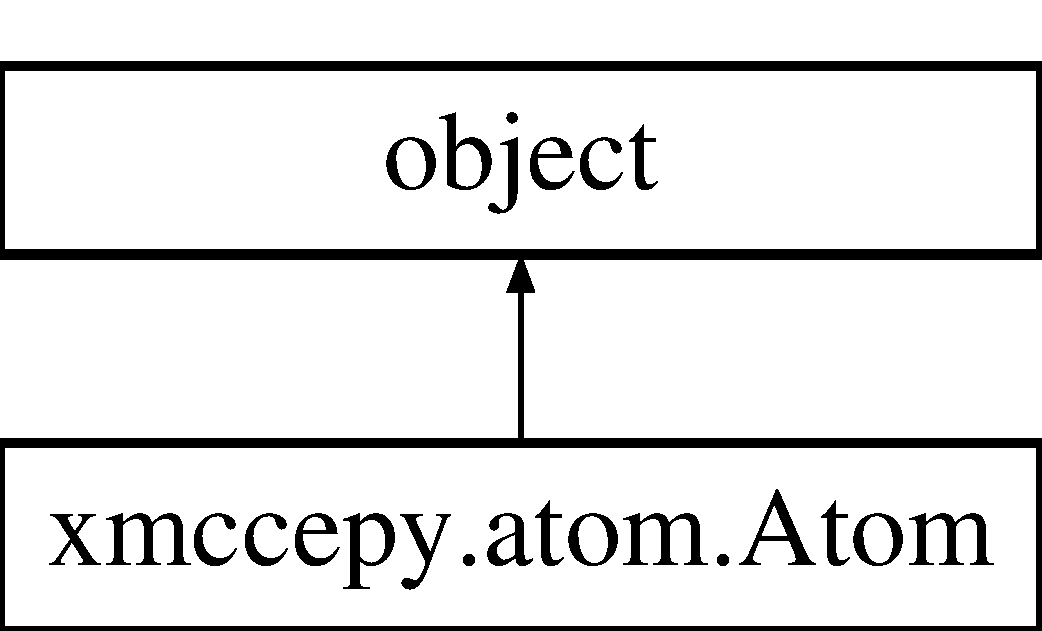
\includegraphics[height=2.000000cm]{classxmccepy_1_1atom_1_1_atom}
\end{center}
\end{figure}
\subsection*{Public Member Functions}
\begin{DoxyCompactItemize}
\item 
def \hyperlink{classxmccepy_1_1atom_1_1_atom_a1964c39c0d09b6867c35ad3ad95c4f06}{\-\_\-\-\_\-init\-\_\-\-\_\-}
\begin{DoxyCompactList}\small\item\em Constructor. \end{DoxyCompactList}\item 
def \hyperlink{classxmccepy_1_1atom_1_1_atom_ae2e395a615e79abe1dd1c5f0ce3d0c90}{set\-Corr}
\begin{DoxyCompactList}\small\item\em Set the coordinate of the atom. \end{DoxyCompactList}\item 
def \hyperlink{classxmccepy_1_1atom_1_1_atom_af43673725714087009243eadbc7f95a7}{read\-Step1\-Line}
\begin{DoxyCompactList}\small\item\em Read a line in step1\-\_\-out.\-pdb. \end{DoxyCompactList}\item 
def \hyperlink{classxmccepy_1_1atom_1_1_atom_a5f3516b8720c26ba0712f7b6066c1cf4}{write\-Step1\-Line}
\begin{DoxyCompactList}\small\item\em Write atom like a line in step1\-\_\-out.\-pdb. \end{DoxyCompactList}\item 
def \hyperlink{classxmccepy_1_1atom_1_1_atom_a36929050f7e6a8728a3525a3eb58b044}{read\-Pdb\-Line}
\begin{DoxyCompactList}\small\item\em Read a line in a standard pdb file. \end{DoxyCompactList}\item 
def \hyperlink{classxmccepy_1_1atom_1_1_atom_a19708571103d9d925eaa23d07a7963d8}{write\-Pdb\-Line}
\begin{DoxyCompactList}\small\item\em Write atom like a line in standard pdb file. \end{DoxyCompactList}\end{DoxyCompactItemize}
\subsection*{Public Attributes}
\begin{DoxyCompactItemize}
\item 
\hyperlink{classxmccepy_1_1atom_1_1_atom_ad394fcd2eca6340dcd5d832a1bd0ec8a}{group\-Id}
\begin{DoxyCompactList}\small\item\em A\-T\-O\-M or H\-E\-T\-A\-T\-M. \end{DoxyCompactList}\item 
\hyperlink{classxmccepy_1_1atom_1_1_atom_a4c4c032cdb4a5f7e5df6f78c10d11629}{atom\-Seq}
\item 
\hyperlink{classxmccepy_1_1atom_1_1_atom_a410419d5a7bcf8e5bb504c393c03849f}{atom\-Name}
\begin{DoxyCompactList}\small\item\em Four letter standard name as in tpl file. \end{DoxyCompactList}\item 
\hyperlink{classxmccepy_1_1atom_1_1_atom_a7fe1185c33a55254824b54ef1218de51}{res\-Name}
\item 
\hyperlink{classxmccepy_1_1atom_1_1_atom_acd780de97bd09f7eba1a6f1067badbf0}{chain\-Id}
\item 
\hyperlink{classxmccepy_1_1atom_1_1_atom_a539eb962040217d58384463edbc73718}{res\-Seq}
\item 
\hyperlink{classxmccepy_1_1atom_1_1_atom_af11e5763e17aa49dd9ceeb73496a3eb5}{conf\-Seq}
\item 
\hyperlink{classxmccepy_1_1atom_1_1_atom_af3e01f96338f93fbcc67765c4d668066}{corr}
\item 
\hyperlink{classxmccepy_1_1atom_1_1_atom_af0235fff236afb4e97011731adb22f55}{radius}
\item 
\hyperlink{classxmccepy_1_1atom_1_1_atom_a75da5d014806b57f4bc26095aa5f8c80}{charge}
\item 
\hyperlink{classxmccepy_1_1atom_1_1_atom_a40df064eecfddbd9a84044c42742ca53}{history}
\item 
\hyperlink{classxmccepy_1_1atom_1_1_atom_a0ae57fea9163a481424524a4a57fb1de}{pdb\-Rest}
\begin{DoxyCompactList}\small\item\em The trailing part of a pdb line which is not parsed. \end{DoxyCompactList}\end{DoxyCompactItemize}


\subsection{Detailed Description}
\hyperlink{classxmccepy_1_1atom_1_1_atom}{Atom} class. 

\subsection{Constructor \& Destructor Documentation}
\hypertarget{classxmccepy_1_1atom_1_1_atom_a1964c39c0d09b6867c35ad3ad95c4f06}{\index{xmccepy\-::atom\-::\-Atom@{xmccepy\-::atom\-::\-Atom}!\-\_\-\-\_\-init\-\_\-\-\_\-@{\-\_\-\-\_\-init\-\_\-\-\_\-}}
\index{\-\_\-\-\_\-init\-\_\-\-\_\-@{\-\_\-\-\_\-init\-\_\-\-\_\-}!xmccepy::atom::Atom@{xmccepy\-::atom\-::\-Atom}}
\subsubsection[{\-\_\-\-\_\-init\-\_\-\-\_\-}]{\setlength{\rightskip}{0pt plus 5cm}def xmccepy.\-atom.\-Atom.\-\_\-\-\_\-init\-\_\-\-\_\- (
\begin{DoxyParamCaption}
\item[{}]{self}
\end{DoxyParamCaption}
)}}\label{classxmccepy_1_1atom_1_1_atom_a1964c39c0d09b6867c35ad3ad95c4f06}


Constructor. 



\subsection{Member Function Documentation}
\hypertarget{classxmccepy_1_1atom_1_1_atom_a36929050f7e6a8728a3525a3eb58b044}{\index{xmccepy\-::atom\-::\-Atom@{xmccepy\-::atom\-::\-Atom}!read\-Pdb\-Line@{read\-Pdb\-Line}}
\index{read\-Pdb\-Line@{read\-Pdb\-Line}!xmccepy::atom::Atom@{xmccepy\-::atom\-::\-Atom}}
\subsubsection[{read\-Pdb\-Line}]{\setlength{\rightskip}{0pt plus 5cm}def xmccepy.\-atom.\-Atom.\-read\-Pdb\-Line (
\begin{DoxyParamCaption}
\item[{}]{self, }
\item[{}]{pline}
\end{DoxyParamCaption}
)}}\label{classxmccepy_1_1atom_1_1_atom_a36929050f7e6a8728a3525a3eb58b044}


Read a line in a standard pdb file. 


\begin{DoxyParams}{Parameters}
{\em pline} & A line in pdb file. \\
\hline
\end{DoxyParams}
\hypertarget{classxmccepy_1_1atom_1_1_atom_af43673725714087009243eadbc7f95a7}{\index{xmccepy\-::atom\-::\-Atom@{xmccepy\-::atom\-::\-Atom}!read\-Step1\-Line@{read\-Step1\-Line}}
\index{read\-Step1\-Line@{read\-Step1\-Line}!xmccepy::atom::Atom@{xmccepy\-::atom\-::\-Atom}}
\subsubsection[{read\-Step1\-Line}]{\setlength{\rightskip}{0pt plus 5cm}def xmccepy.\-atom.\-Atom.\-read\-Step1\-Line (
\begin{DoxyParamCaption}
\item[{}]{self, }
\item[{}]{sline}
\end{DoxyParamCaption}
)}}\label{classxmccepy_1_1atom_1_1_atom_af43673725714087009243eadbc7f95a7}


Read a line in step1\-\_\-out.\-pdb. 

A line in step1\-\_\-out.\-pdb represents an atom with extra info about the conformer. 
\begin{DoxyParams}{Parameters}
{\em sline} & A line from step1\-\_\-out.\-pdb. \\
\hline
\end{DoxyParams}
\hypertarget{classxmccepy_1_1atom_1_1_atom_ae2e395a615e79abe1dd1c5f0ce3d0c90}{\index{xmccepy\-::atom\-::\-Atom@{xmccepy\-::atom\-::\-Atom}!set\-Corr@{set\-Corr}}
\index{set\-Corr@{set\-Corr}!xmccepy::atom::Atom@{xmccepy\-::atom\-::\-Atom}}
\subsubsection[{set\-Corr}]{\setlength{\rightskip}{0pt plus 5cm}def xmccepy.\-atom.\-Atom.\-set\-Corr (
\begin{DoxyParamCaption}
\item[{}]{self, }
\item[{}]{x = {\ttfamily 0.0}, }
\item[{}]{y = {\ttfamily 0.0}, }
\item[{}]{z = {\ttfamily 0.0}}
\end{DoxyParamCaption}
)}}\label{classxmccepy_1_1atom_1_1_atom_ae2e395a615e79abe1dd1c5f0ce3d0c90}


Set the coordinate of the atom. 

\hypertarget{classxmccepy_1_1atom_1_1_atom_a19708571103d9d925eaa23d07a7963d8}{\index{xmccepy\-::atom\-::\-Atom@{xmccepy\-::atom\-::\-Atom}!write\-Pdb\-Line@{write\-Pdb\-Line}}
\index{write\-Pdb\-Line@{write\-Pdb\-Line}!xmccepy::atom::Atom@{xmccepy\-::atom\-::\-Atom}}
\subsubsection[{write\-Pdb\-Line}]{\setlength{\rightskip}{0pt plus 5cm}def xmccepy.\-atom.\-Atom.\-write\-Pdb\-Line (
\begin{DoxyParamCaption}
\item[{}]{self}
\end{DoxyParamCaption}
)}}\label{classxmccepy_1_1atom_1_1_atom_a19708571103d9d925eaa23d07a7963d8}


Write atom like a line in standard pdb file. 

\begin{DoxyReturn}{Returns}
A line of atom for pdb file. 
\end{DoxyReturn}
\hypertarget{classxmccepy_1_1atom_1_1_atom_a5f3516b8720c26ba0712f7b6066c1cf4}{\index{xmccepy\-::atom\-::\-Atom@{xmccepy\-::atom\-::\-Atom}!write\-Step1\-Line@{write\-Step1\-Line}}
\index{write\-Step1\-Line@{write\-Step1\-Line}!xmccepy::atom::Atom@{xmccepy\-::atom\-::\-Atom}}
\subsubsection[{write\-Step1\-Line}]{\setlength{\rightskip}{0pt plus 5cm}def xmccepy.\-atom.\-Atom.\-write\-Step1\-Line (
\begin{DoxyParamCaption}
\item[{}]{self}
\end{DoxyParamCaption}
)}}\label{classxmccepy_1_1atom_1_1_atom_a5f3516b8720c26ba0712f7b6066c1cf4}


Write atom like a line in step1\-\_\-out.\-pdb. 

\begin{DoxyReturn}{Returns}
A line of atom for step1\-\_\-out.\-pdb. 
\end{DoxyReturn}


\subsection{Member Data Documentation}
\hypertarget{classxmccepy_1_1atom_1_1_atom_a410419d5a7bcf8e5bb504c393c03849f}{\index{xmccepy\-::atom\-::\-Atom@{xmccepy\-::atom\-::\-Atom}!atom\-Name@{atom\-Name}}
\index{atom\-Name@{atom\-Name}!xmccepy::atom::Atom@{xmccepy\-::atom\-::\-Atom}}
\subsubsection[{atom\-Name}]{\setlength{\rightskip}{0pt plus 5cm}xmccepy.\-atom.\-Atom.\-atom\-Name}}\label{classxmccepy_1_1atom_1_1_atom_a410419d5a7bcf8e5bb504c393c03849f}


Four letter standard name as in tpl file. 

\hypertarget{classxmccepy_1_1atom_1_1_atom_a4c4c032cdb4a5f7e5df6f78c10d11629}{\index{xmccepy\-::atom\-::\-Atom@{xmccepy\-::atom\-::\-Atom}!atom\-Seq@{atom\-Seq}}
\index{atom\-Seq@{atom\-Seq}!xmccepy::atom::Atom@{xmccepy\-::atom\-::\-Atom}}
\subsubsection[{atom\-Seq}]{\setlength{\rightskip}{0pt plus 5cm}xmccepy.\-atom.\-Atom.\-atom\-Seq}}\label{classxmccepy_1_1atom_1_1_atom_a4c4c032cdb4a5f7e5df6f78c10d11629}
\hypertarget{classxmccepy_1_1atom_1_1_atom_acd780de97bd09f7eba1a6f1067badbf0}{\index{xmccepy\-::atom\-::\-Atom@{xmccepy\-::atom\-::\-Atom}!chain\-Id@{chain\-Id}}
\index{chain\-Id@{chain\-Id}!xmccepy::atom::Atom@{xmccepy\-::atom\-::\-Atom}}
\subsubsection[{chain\-Id}]{\setlength{\rightskip}{0pt plus 5cm}xmccepy.\-atom.\-Atom.\-chain\-Id}}\label{classxmccepy_1_1atom_1_1_atom_acd780de97bd09f7eba1a6f1067badbf0}
\hypertarget{classxmccepy_1_1atom_1_1_atom_a75da5d014806b57f4bc26095aa5f8c80}{\index{xmccepy\-::atom\-::\-Atom@{xmccepy\-::atom\-::\-Atom}!charge@{charge}}
\index{charge@{charge}!xmccepy::atom::Atom@{xmccepy\-::atom\-::\-Atom}}
\subsubsection[{charge}]{\setlength{\rightskip}{0pt plus 5cm}xmccepy.\-atom.\-Atom.\-charge}}\label{classxmccepy_1_1atom_1_1_atom_a75da5d014806b57f4bc26095aa5f8c80}
\hypertarget{classxmccepy_1_1atom_1_1_atom_af11e5763e17aa49dd9ceeb73496a3eb5}{\index{xmccepy\-::atom\-::\-Atom@{xmccepy\-::atom\-::\-Atom}!conf\-Seq@{conf\-Seq}}
\index{conf\-Seq@{conf\-Seq}!xmccepy::atom::Atom@{xmccepy\-::atom\-::\-Atom}}
\subsubsection[{conf\-Seq}]{\setlength{\rightskip}{0pt plus 5cm}xmccepy.\-atom.\-Atom.\-conf\-Seq}}\label{classxmccepy_1_1atom_1_1_atom_af11e5763e17aa49dd9ceeb73496a3eb5}
\hypertarget{classxmccepy_1_1atom_1_1_atom_af3e01f96338f93fbcc67765c4d668066}{\index{xmccepy\-::atom\-::\-Atom@{xmccepy\-::atom\-::\-Atom}!corr@{corr}}
\index{corr@{corr}!xmccepy::atom::Atom@{xmccepy\-::atom\-::\-Atom}}
\subsubsection[{corr}]{\setlength{\rightskip}{0pt plus 5cm}xmccepy.\-atom.\-Atom.\-corr}}\label{classxmccepy_1_1atom_1_1_atom_af3e01f96338f93fbcc67765c4d668066}
\hypertarget{classxmccepy_1_1atom_1_1_atom_ad394fcd2eca6340dcd5d832a1bd0ec8a}{\index{xmccepy\-::atom\-::\-Atom@{xmccepy\-::atom\-::\-Atom}!group\-Id@{group\-Id}}
\index{group\-Id@{group\-Id}!xmccepy::atom::Atom@{xmccepy\-::atom\-::\-Atom}}
\subsubsection[{group\-Id}]{\setlength{\rightskip}{0pt plus 5cm}xmccepy.\-atom.\-Atom.\-group\-Id}}\label{classxmccepy_1_1atom_1_1_atom_ad394fcd2eca6340dcd5d832a1bd0ec8a}


A\-T\-O\-M or H\-E\-T\-A\-T\-M. 

\hypertarget{classxmccepy_1_1atom_1_1_atom_a40df064eecfddbd9a84044c42742ca53}{\index{xmccepy\-::atom\-::\-Atom@{xmccepy\-::atom\-::\-Atom}!history@{history}}
\index{history@{history}!xmccepy::atom::Atom@{xmccepy\-::atom\-::\-Atom}}
\subsubsection[{history}]{\setlength{\rightskip}{0pt plus 5cm}xmccepy.\-atom.\-Atom.\-history}}\label{classxmccepy_1_1atom_1_1_atom_a40df064eecfddbd9a84044c42742ca53}
\hypertarget{classxmccepy_1_1atom_1_1_atom_a0ae57fea9163a481424524a4a57fb1de}{\index{xmccepy\-::atom\-::\-Atom@{xmccepy\-::atom\-::\-Atom}!pdb\-Rest@{pdb\-Rest}}
\index{pdb\-Rest@{pdb\-Rest}!xmccepy::atom::Atom@{xmccepy\-::atom\-::\-Atom}}
\subsubsection[{pdb\-Rest}]{\setlength{\rightskip}{0pt plus 5cm}xmccepy.\-atom.\-Atom.\-pdb\-Rest}}\label{classxmccepy_1_1atom_1_1_atom_a0ae57fea9163a481424524a4a57fb1de}


The trailing part of a pdb line which is not parsed. 

\hypertarget{classxmccepy_1_1atom_1_1_atom_af0235fff236afb4e97011731adb22f55}{\index{xmccepy\-::atom\-::\-Atom@{xmccepy\-::atom\-::\-Atom}!radius@{radius}}
\index{radius@{radius}!xmccepy::atom::Atom@{xmccepy\-::atom\-::\-Atom}}
\subsubsection[{radius}]{\setlength{\rightskip}{0pt plus 5cm}xmccepy.\-atom.\-Atom.\-radius}}\label{classxmccepy_1_1atom_1_1_atom_af0235fff236afb4e97011731adb22f55}
\hypertarget{classxmccepy_1_1atom_1_1_atom_a7fe1185c33a55254824b54ef1218de51}{\index{xmccepy\-::atom\-::\-Atom@{xmccepy\-::atom\-::\-Atom}!res\-Name@{res\-Name}}
\index{res\-Name@{res\-Name}!xmccepy::atom::Atom@{xmccepy\-::atom\-::\-Atom}}
\subsubsection[{res\-Name}]{\setlength{\rightskip}{0pt plus 5cm}xmccepy.\-atom.\-Atom.\-res\-Name}}\label{classxmccepy_1_1atom_1_1_atom_a7fe1185c33a55254824b54ef1218de51}
\hypertarget{classxmccepy_1_1atom_1_1_atom_a539eb962040217d58384463edbc73718}{\index{xmccepy\-::atom\-::\-Atom@{xmccepy\-::atom\-::\-Atom}!res\-Seq@{res\-Seq}}
\index{res\-Seq@{res\-Seq}!xmccepy::atom::Atom@{xmccepy\-::atom\-::\-Atom}}
\subsubsection[{res\-Seq}]{\setlength{\rightskip}{0pt plus 5cm}xmccepy.\-atom.\-Atom.\-res\-Seq}}\label{classxmccepy_1_1atom_1_1_atom_a539eb962040217d58384463edbc73718}


The documentation for this class was generated from the following file\-:\begin{DoxyCompactItemize}
\item 
src/xmccepy/\hyperlink{atom_8py}{atom.\-py}\end{DoxyCompactItemize}

\hypertarget{classxmccepy_1_1mp_1_1_a_t_o_m}{\section{xmccepy.\-mp.\-A\-T\-O\-M Class Reference}
\label{classxmccepy_1_1mp_1_1_a_t_o_m}\index{xmccepy.\-mp.\-A\-T\-O\-M@{xmccepy.\-mp.\-A\-T\-O\-M}}
}
\subsection*{Public Member Functions}
\begin{DoxyCompactItemize}
\item 
def \hyperlink{classxmccepy_1_1mp_1_1_a_t_o_m_aa6e2fb4b7c8efc44b26b2b21964db907}{\-\_\-\-\_\-init\-\_\-\-\_\-}
\item 
def \hyperlink{classxmccepy_1_1mp_1_1_a_t_o_m_a136255ca36ba6682255e0c3c16b49c39}{load\-Step\-Line}
\end{DoxyCompactItemize}
\subsection*{Public Attributes}
\begin{DoxyCompactItemize}
\item 
\hyperlink{classxmccepy_1_1mp_1_1_a_t_o_m_a2cef52139b5235586607f4ba6fe44ee9}{serial}
\item 
\hyperlink{classxmccepy_1_1mp_1_1_a_t_o_m_a54ade2663ba22d42473d82bbb0731451}{name}
\item 
\hyperlink{classxmccepy_1_1mp_1_1_a_t_o_m_afbc19b6c21ca49dbe761479669a24c66}{alt\-Loc}
\item 
\hyperlink{classxmccepy_1_1mp_1_1_a_t_o_m_a8f4bed4463123a6d83abd93f69438ebe}{res\-Name}
\item 
\hyperlink{classxmccepy_1_1mp_1_1_a_t_o_m_a253ac66ab99349121fda0a6183f10a12}{chain\-I\-D}
\item 
\hyperlink{classxmccepy_1_1mp_1_1_a_t_o_m_ac91c801a2d8279659c74c69e820215a9}{res\-Seq}
\item 
\hyperlink{classxmccepy_1_1mp_1_1_a_t_o_m_a7ace60261d88bcbcd23f5e14a86b77e6}{i\-Code}
\item 
\hyperlink{classxmccepy_1_1mp_1_1_a_t_o_m_aebf9f0b985ccd236b1cd2dbf1161941e}{xyz}
\item 
\hyperlink{classxmccepy_1_1mp_1_1_a_t_o_m_ae56b3a55f15835108b393b32f6ac1878}{rad}
\item 
\hyperlink{classxmccepy_1_1mp_1_1_a_t_o_m_a0e3bac6ace5f4cc33db8eb20120764d4}{crg}
\item 
\hyperlink{classxmccepy_1_1mp_1_1_a_t_o_m_aa3702294f6091d253474476bfcd35f34}{history}
\end{DoxyCompactItemize}


\subsection{Constructor \& Destructor Documentation}
\hypertarget{classxmccepy_1_1mp_1_1_a_t_o_m_aa6e2fb4b7c8efc44b26b2b21964db907}{\index{xmccepy\-::mp\-::\-A\-T\-O\-M@{xmccepy\-::mp\-::\-A\-T\-O\-M}!\-\_\-\-\_\-init\-\_\-\-\_\-@{\-\_\-\-\_\-init\-\_\-\-\_\-}}
\index{\-\_\-\-\_\-init\-\_\-\-\_\-@{\-\_\-\-\_\-init\-\_\-\-\_\-}!xmccepy::mp::ATOM@{xmccepy\-::mp\-::\-A\-T\-O\-M}}
\subsubsection[{\-\_\-\-\_\-init\-\_\-\-\_\-}]{\setlength{\rightskip}{0pt plus 5cm}def xmccepy.\-mp.\-A\-T\-O\-M.\-\_\-\-\_\-init\-\_\-\-\_\- (
\begin{DoxyParamCaption}
\item[{}]{self}
\end{DoxyParamCaption}
)}}\label{classxmccepy_1_1mp_1_1_a_t_o_m_aa6e2fb4b7c8efc44b26b2b21964db907}


\subsection{Member Function Documentation}
\hypertarget{classxmccepy_1_1mp_1_1_a_t_o_m_a136255ca36ba6682255e0c3c16b49c39}{\index{xmccepy\-::mp\-::\-A\-T\-O\-M@{xmccepy\-::mp\-::\-A\-T\-O\-M}!load\-Step\-Line@{load\-Step\-Line}}
\index{load\-Step\-Line@{load\-Step\-Line}!xmccepy::mp::ATOM@{xmccepy\-::mp\-::\-A\-T\-O\-M}}
\subsubsection[{load\-Step\-Line}]{\setlength{\rightskip}{0pt plus 5cm}def xmccepy.\-mp.\-A\-T\-O\-M.\-load\-Step\-Line (
\begin{DoxyParamCaption}
\item[{}]{self, }
\item[{}]{line}
\end{DoxyParamCaption}
)}}\label{classxmccepy_1_1mp_1_1_a_t_o_m_a136255ca36ba6682255e0c3c16b49c39}


\subsection{Member Data Documentation}
\hypertarget{classxmccepy_1_1mp_1_1_a_t_o_m_afbc19b6c21ca49dbe761479669a24c66}{\index{xmccepy\-::mp\-::\-A\-T\-O\-M@{xmccepy\-::mp\-::\-A\-T\-O\-M}!alt\-Loc@{alt\-Loc}}
\index{alt\-Loc@{alt\-Loc}!xmccepy::mp::ATOM@{xmccepy\-::mp\-::\-A\-T\-O\-M}}
\subsubsection[{alt\-Loc}]{\setlength{\rightskip}{0pt plus 5cm}xmccepy.\-mp.\-A\-T\-O\-M.\-alt\-Loc}}\label{classxmccepy_1_1mp_1_1_a_t_o_m_afbc19b6c21ca49dbe761479669a24c66}
\hypertarget{classxmccepy_1_1mp_1_1_a_t_o_m_a253ac66ab99349121fda0a6183f10a12}{\index{xmccepy\-::mp\-::\-A\-T\-O\-M@{xmccepy\-::mp\-::\-A\-T\-O\-M}!chain\-I\-D@{chain\-I\-D}}
\index{chain\-I\-D@{chain\-I\-D}!xmccepy::mp::ATOM@{xmccepy\-::mp\-::\-A\-T\-O\-M}}
\subsubsection[{chain\-I\-D}]{\setlength{\rightskip}{0pt plus 5cm}xmccepy.\-mp.\-A\-T\-O\-M.\-chain\-I\-D}}\label{classxmccepy_1_1mp_1_1_a_t_o_m_a253ac66ab99349121fda0a6183f10a12}
\hypertarget{classxmccepy_1_1mp_1_1_a_t_o_m_a0e3bac6ace5f4cc33db8eb20120764d4}{\index{xmccepy\-::mp\-::\-A\-T\-O\-M@{xmccepy\-::mp\-::\-A\-T\-O\-M}!crg@{crg}}
\index{crg@{crg}!xmccepy::mp::ATOM@{xmccepy\-::mp\-::\-A\-T\-O\-M}}
\subsubsection[{crg}]{\setlength{\rightskip}{0pt plus 5cm}xmccepy.\-mp.\-A\-T\-O\-M.\-crg}}\label{classxmccepy_1_1mp_1_1_a_t_o_m_a0e3bac6ace5f4cc33db8eb20120764d4}
\hypertarget{classxmccepy_1_1mp_1_1_a_t_o_m_aa3702294f6091d253474476bfcd35f34}{\index{xmccepy\-::mp\-::\-A\-T\-O\-M@{xmccepy\-::mp\-::\-A\-T\-O\-M}!history@{history}}
\index{history@{history}!xmccepy::mp::ATOM@{xmccepy\-::mp\-::\-A\-T\-O\-M}}
\subsubsection[{history}]{\setlength{\rightskip}{0pt plus 5cm}xmccepy.\-mp.\-A\-T\-O\-M.\-history}}\label{classxmccepy_1_1mp_1_1_a_t_o_m_aa3702294f6091d253474476bfcd35f34}
\hypertarget{classxmccepy_1_1mp_1_1_a_t_o_m_a7ace60261d88bcbcd23f5e14a86b77e6}{\index{xmccepy\-::mp\-::\-A\-T\-O\-M@{xmccepy\-::mp\-::\-A\-T\-O\-M}!i\-Code@{i\-Code}}
\index{i\-Code@{i\-Code}!xmccepy::mp::ATOM@{xmccepy\-::mp\-::\-A\-T\-O\-M}}
\subsubsection[{i\-Code}]{\setlength{\rightskip}{0pt plus 5cm}xmccepy.\-mp.\-A\-T\-O\-M.\-i\-Code}}\label{classxmccepy_1_1mp_1_1_a_t_o_m_a7ace60261d88bcbcd23f5e14a86b77e6}
\hypertarget{classxmccepy_1_1mp_1_1_a_t_o_m_a54ade2663ba22d42473d82bbb0731451}{\index{xmccepy\-::mp\-::\-A\-T\-O\-M@{xmccepy\-::mp\-::\-A\-T\-O\-M}!name@{name}}
\index{name@{name}!xmccepy::mp::ATOM@{xmccepy\-::mp\-::\-A\-T\-O\-M}}
\subsubsection[{name}]{\setlength{\rightskip}{0pt plus 5cm}xmccepy.\-mp.\-A\-T\-O\-M.\-name}}\label{classxmccepy_1_1mp_1_1_a_t_o_m_a54ade2663ba22d42473d82bbb0731451}
\hypertarget{classxmccepy_1_1mp_1_1_a_t_o_m_ae56b3a55f15835108b393b32f6ac1878}{\index{xmccepy\-::mp\-::\-A\-T\-O\-M@{xmccepy\-::mp\-::\-A\-T\-O\-M}!rad@{rad}}
\index{rad@{rad}!xmccepy::mp::ATOM@{xmccepy\-::mp\-::\-A\-T\-O\-M}}
\subsubsection[{rad}]{\setlength{\rightskip}{0pt plus 5cm}xmccepy.\-mp.\-A\-T\-O\-M.\-rad}}\label{classxmccepy_1_1mp_1_1_a_t_o_m_ae56b3a55f15835108b393b32f6ac1878}
\hypertarget{classxmccepy_1_1mp_1_1_a_t_o_m_a8f4bed4463123a6d83abd93f69438ebe}{\index{xmccepy\-::mp\-::\-A\-T\-O\-M@{xmccepy\-::mp\-::\-A\-T\-O\-M}!res\-Name@{res\-Name}}
\index{res\-Name@{res\-Name}!xmccepy::mp::ATOM@{xmccepy\-::mp\-::\-A\-T\-O\-M}}
\subsubsection[{res\-Name}]{\setlength{\rightskip}{0pt plus 5cm}xmccepy.\-mp.\-A\-T\-O\-M.\-res\-Name}}\label{classxmccepy_1_1mp_1_1_a_t_o_m_a8f4bed4463123a6d83abd93f69438ebe}
\hypertarget{classxmccepy_1_1mp_1_1_a_t_o_m_ac91c801a2d8279659c74c69e820215a9}{\index{xmccepy\-::mp\-::\-A\-T\-O\-M@{xmccepy\-::mp\-::\-A\-T\-O\-M}!res\-Seq@{res\-Seq}}
\index{res\-Seq@{res\-Seq}!xmccepy::mp::ATOM@{xmccepy\-::mp\-::\-A\-T\-O\-M}}
\subsubsection[{res\-Seq}]{\setlength{\rightskip}{0pt plus 5cm}xmccepy.\-mp.\-A\-T\-O\-M.\-res\-Seq}}\label{classxmccepy_1_1mp_1_1_a_t_o_m_ac91c801a2d8279659c74c69e820215a9}
\hypertarget{classxmccepy_1_1mp_1_1_a_t_o_m_a2cef52139b5235586607f4ba6fe44ee9}{\index{xmccepy\-::mp\-::\-A\-T\-O\-M@{xmccepy\-::mp\-::\-A\-T\-O\-M}!serial@{serial}}
\index{serial@{serial}!xmccepy::mp::ATOM@{xmccepy\-::mp\-::\-A\-T\-O\-M}}
\subsubsection[{serial}]{\setlength{\rightskip}{0pt plus 5cm}xmccepy.\-mp.\-A\-T\-O\-M.\-serial}}\label{classxmccepy_1_1mp_1_1_a_t_o_m_a2cef52139b5235586607f4ba6fe44ee9}
\hypertarget{classxmccepy_1_1mp_1_1_a_t_o_m_aebf9f0b985ccd236b1cd2dbf1161941e}{\index{xmccepy\-::mp\-::\-A\-T\-O\-M@{xmccepy\-::mp\-::\-A\-T\-O\-M}!xyz@{xyz}}
\index{xyz@{xyz}!xmccepy::mp::ATOM@{xmccepy\-::mp\-::\-A\-T\-O\-M}}
\subsubsection[{xyz}]{\setlength{\rightskip}{0pt plus 5cm}xmccepy.\-mp.\-A\-T\-O\-M.\-xyz}}\label{classxmccepy_1_1mp_1_1_a_t_o_m_aebf9f0b985ccd236b1cd2dbf1161941e}


The documentation for this class was generated from the following file\-:\begin{DoxyCompactItemize}
\item 
src/xmccepy/\hyperlink{mp_8py}{mp.\-py}\end{DoxyCompactItemize}

\hypertarget{classatom__hbond_1_1_atom_net}{\section{atom\-\_\-hbond.\-Atom\-Net Class Reference}
\label{classatom__hbond_1_1_atom_net}\index{atom\-\_\-hbond.\-Atom\-Net@{atom\-\_\-hbond.\-Atom\-Net}}
}
Inheritance diagram for atom\-\_\-hbond.\-Atom\-Net\-:\begin{figure}[H]
\begin{center}
\leavevmode
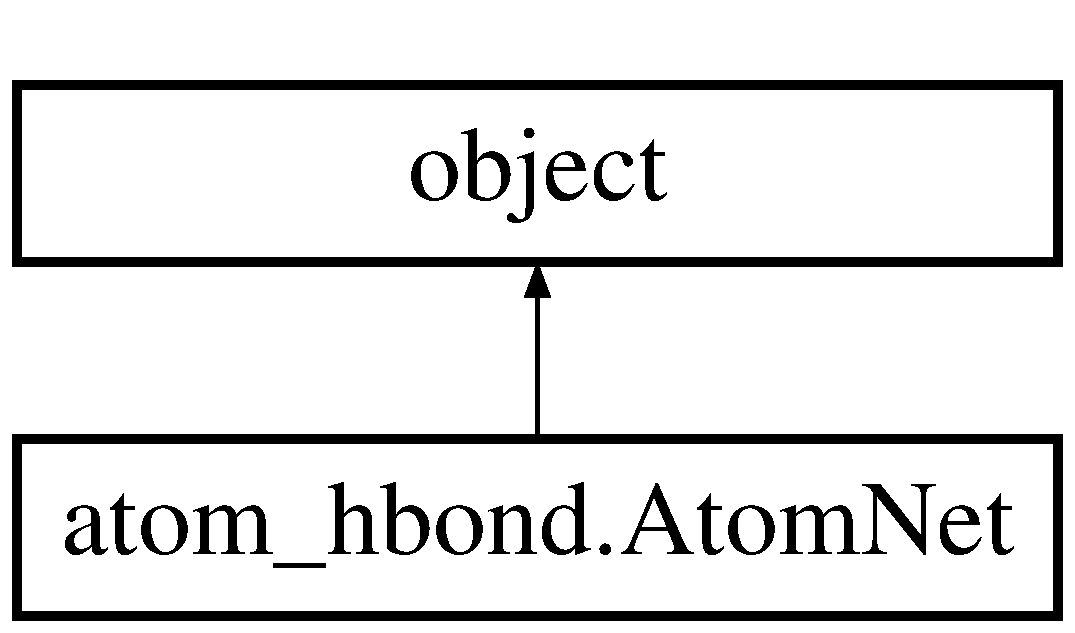
\includegraphics[height=2.000000cm]{classatom__hbond_1_1_atom_net}
\end{center}
\end{figure}
\subsection*{Public Member Functions}
\begin{DoxyCompactItemize}
\item 
def \hyperlink{classatom__hbond_1_1_atom_net_a2aa26477e40c03bf66d516543af1ae94}{\-\_\-\-\_\-init\-\_\-\-\_\-}
\item 
def \hyperlink{classatom__hbond_1_1_atom_net_ace5c54516014e2987b5335b85bfec60d}{obtain\-Network\-From\-File}
\begin{DoxyCompactList}\small\item\em Get the atom network from \char`\"{}hah.\-txt\char`\"{} file. \end{DoxyCompactList}\item 
def \hyperlink{classatom__hbond_1_1_atom_net_a7cdc5e4dfc0d48c1312520fddf1ba3c0}{obtain\-Network\-With\-Occ}
\item 
def \hyperlink{classatom__hbond_1_1_atom_net_ac8b24f543113377688d1a2b9ed0f9c89}{store\-In\-File}
\begin{DoxyCompactList}\small\item\em Store the atom network in a file named \char`\"{}atomhb.\-txt\char`\"{}. \end{DoxyCompactList}\item 
def \hyperlink{classatom__hbond_1_1_atom_net_af218b8037988a7ba5df0e158981dd890}{store\-\_\-atomreshb}
\begin{DoxyCompactList}\small\item\em Store the atom network in a file named \char`\"{}atomhb.\-txt\char`\"{}. \end{DoxyCompactList}\item 
def \hyperlink{classatom__hbond_1_1_atom_net_a14de518f576bf0a42a6017d9ab62ba7d}{load\-Graph}
\begin{DoxyCompactList}\small\item\em Get the atom network from \char`\"{}atomhb.\-txt\char`\"{} file, which has been written to store an atom network. \end{DoxyCompactList}\item 
def \hyperlink{classatom__hbond_1_1_atom_net_ae66207e59bb231d976218a04c183c088}{print\-Shortest\-Path}
\item 
def \hyperlink{classatom__hbond_1_1_atom_net_accacb11bbd9165cabde21f8c7765fd30}{shortest\-Path\-Between\-Residues}
\begin{DoxyCompactList}\small\item\em Get a shortest pathway between each donor atom in source\-Res and each acceptor atom in target\-Res, if there exists. \end{DoxyCompactList}\end{DoxyCompactItemize}
\subsection*{Public Attributes}
\begin{DoxyCompactItemize}
\item 
\hyperlink{classatom__hbond_1_1_atom_net_a9b13bfbc0ec665e7f5dcddd4bf74fee2}{g}
\end{DoxyCompactItemize}


\subsection{Constructor \& Destructor Documentation}
\hypertarget{classatom__hbond_1_1_atom_net_a2aa26477e40c03bf66d516543af1ae94}{\index{atom\-\_\-hbond\-::\-Atom\-Net@{atom\-\_\-hbond\-::\-Atom\-Net}!\-\_\-\-\_\-init\-\_\-\-\_\-@{\-\_\-\-\_\-init\-\_\-\-\_\-}}
\index{\-\_\-\-\_\-init\-\_\-\-\_\-@{\-\_\-\-\_\-init\-\_\-\-\_\-}!atom_hbond::AtomNet@{atom\-\_\-hbond\-::\-Atom\-Net}}
\subsubsection[{\-\_\-\-\_\-init\-\_\-\-\_\-}]{\setlength{\rightskip}{0pt plus 5cm}def atom\-\_\-hbond.\-Atom\-Net.\-\_\-\-\_\-init\-\_\-\-\_\- (
\begin{DoxyParamCaption}
\item[{}]{self}
\end{DoxyParamCaption}
)}}\label{classatom__hbond_1_1_atom_net_a2aa26477e40c03bf66d516543af1ae94}


\subsection{Member Function Documentation}
\hypertarget{classatom__hbond_1_1_atom_net_a14de518f576bf0a42a6017d9ab62ba7d}{\index{atom\-\_\-hbond\-::\-Atom\-Net@{atom\-\_\-hbond\-::\-Atom\-Net}!load\-Graph@{load\-Graph}}
\index{load\-Graph@{load\-Graph}!atom_hbond::AtomNet@{atom\-\_\-hbond\-::\-Atom\-Net}}
\subsubsection[{load\-Graph}]{\setlength{\rightskip}{0pt plus 5cm}def atom\-\_\-hbond.\-Atom\-Net.\-load\-Graph (
\begin{DoxyParamCaption}
\item[{}]{self, }
\item[{}]{f\-Name = {\ttfamily \char`\"{}atomhb.txt\char`\"{}}}
\end{DoxyParamCaption}
)}}\label{classatom__hbond_1_1_atom_net_a14de518f576bf0a42a6017d9ab62ba7d}


Get the atom network from \char`\"{}atomhb.\-txt\char`\"{} file, which has been written to store an atom network. 

\hypertarget{classatom__hbond_1_1_atom_net_ace5c54516014e2987b5335b85bfec60d}{\index{atom\-\_\-hbond\-::\-Atom\-Net@{atom\-\_\-hbond\-::\-Atom\-Net}!obtain\-Network\-From\-File@{obtain\-Network\-From\-File}}
\index{obtain\-Network\-From\-File@{obtain\-Network\-From\-File}!atom_hbond::AtomNet@{atom\-\_\-hbond\-::\-Atom\-Net}}
\subsubsection[{obtain\-Network\-From\-File}]{\setlength{\rightskip}{0pt plus 5cm}def atom\-\_\-hbond.\-Atom\-Net.\-obtain\-Network\-From\-File (
\begin{DoxyParamCaption}
\item[{}]{self, }
\item[{}]{f\-Name = {\ttfamily \char`\"{}hah.txt\char`\"{}}}
\end{DoxyParamCaption}
)}}\label{classatom__hbond_1_1_atom_net_ace5c54516014e2987b5335b85bfec60d}


Get the atom network from \char`\"{}hah.\-txt\char`\"{} file. 

\hypertarget{classatom__hbond_1_1_atom_net_a7cdc5e4dfc0d48c1312520fddf1ba3c0}{\index{atom\-\_\-hbond\-::\-Atom\-Net@{atom\-\_\-hbond\-::\-Atom\-Net}!obtain\-Network\-With\-Occ@{obtain\-Network\-With\-Occ}}
\index{obtain\-Network\-With\-Occ@{obtain\-Network\-With\-Occ}!atom_hbond::AtomNet@{atom\-\_\-hbond\-::\-Atom\-Net}}
\subsubsection[{obtain\-Network\-With\-Occ}]{\setlength{\rightskip}{0pt plus 5cm}def atom\-\_\-hbond.\-Atom\-Net.\-obtain\-Network\-With\-Occ (
\begin{DoxyParamCaption}
\item[{}]{self, }
\item[{}]{f\-Name = {\ttfamily \char`\"{}hah.txt\char`\"{}}, }
\item[{}]{occ\-File = {\ttfamily \char`\"{}fort.38\char`\"{}}}
\end{DoxyParamCaption}
)}}\label{classatom__hbond_1_1_atom_net_a7cdc5e4dfc0d48c1312520fddf1ba3c0}
\hypertarget{classatom__hbond_1_1_atom_net_ae66207e59bb231d976218a04c183c088}{\index{atom\-\_\-hbond\-::\-Atom\-Net@{atom\-\_\-hbond\-::\-Atom\-Net}!print\-Shortest\-Path@{print\-Shortest\-Path}}
\index{print\-Shortest\-Path@{print\-Shortest\-Path}!atom_hbond::AtomNet@{atom\-\_\-hbond\-::\-Atom\-Net}}
\subsubsection[{print\-Shortest\-Path}]{\setlength{\rightskip}{0pt plus 5cm}def atom\-\_\-hbond.\-Atom\-Net.\-print\-Shortest\-Path (
\begin{DoxyParamCaption}
\item[{}]{self, }
\item[{}]{source\-Node, }
\item[{}]{target\-Node}
\end{DoxyParamCaption}
)}}\label{classatom__hbond_1_1_atom_net_ae66207e59bb231d976218a04c183c088}
\hypertarget{classatom__hbond_1_1_atom_net_accacb11bbd9165cabde21f8c7765fd30}{\index{atom\-\_\-hbond\-::\-Atom\-Net@{atom\-\_\-hbond\-::\-Atom\-Net}!shortest\-Path\-Between\-Residues@{shortest\-Path\-Between\-Residues}}
\index{shortest\-Path\-Between\-Residues@{shortest\-Path\-Between\-Residues}!atom_hbond::AtomNet@{atom\-\_\-hbond\-::\-Atom\-Net}}
\subsubsection[{shortest\-Path\-Between\-Residues}]{\setlength{\rightskip}{0pt plus 5cm}def atom\-\_\-hbond.\-Atom\-Net.\-shortest\-Path\-Between\-Residues (
\begin{DoxyParamCaption}
\item[{}]{self, }
\item[{}]{source\-Res, }
\item[{}]{target\-Res}
\end{DoxyParamCaption}
)}}\label{classatom__hbond_1_1_atom_net_accacb11bbd9165cabde21f8c7765fd30}


Get a shortest pathway between each donor atom in source\-Res and each acceptor atom in target\-Res, if there exists. 

\hypertarget{classatom__hbond_1_1_atom_net_af218b8037988a7ba5df0e158981dd890}{\index{atom\-\_\-hbond\-::\-Atom\-Net@{atom\-\_\-hbond\-::\-Atom\-Net}!store\-\_\-atomreshb@{store\-\_\-atomreshb}}
\index{store\-\_\-atomreshb@{store\-\_\-atomreshb}!atom_hbond::AtomNet@{atom\-\_\-hbond\-::\-Atom\-Net}}
\subsubsection[{store\-\_\-atomreshb}]{\setlength{\rightskip}{0pt plus 5cm}def atom\-\_\-hbond.\-Atom\-Net.\-store\-\_\-atomreshb (
\begin{DoxyParamCaption}
\item[{}]{self, }
\item[{}]{f\-Name = {\ttfamily \char`\"{}atomhb.txt\char`\"{}}}
\end{DoxyParamCaption}
)}}\label{classatom__hbond_1_1_atom_net_af218b8037988a7ba5df0e158981dd890}


Store the atom network in a file named \char`\"{}atomhb.\-txt\char`\"{}. 

\hypertarget{classatom__hbond_1_1_atom_net_ac8b24f543113377688d1a2b9ed0f9c89}{\index{atom\-\_\-hbond\-::\-Atom\-Net@{atom\-\_\-hbond\-::\-Atom\-Net}!store\-In\-File@{store\-In\-File}}
\index{store\-In\-File@{store\-In\-File}!atom_hbond::AtomNet@{atom\-\_\-hbond\-::\-Atom\-Net}}
\subsubsection[{store\-In\-File}]{\setlength{\rightskip}{0pt plus 5cm}def atom\-\_\-hbond.\-Atom\-Net.\-store\-In\-File (
\begin{DoxyParamCaption}
\item[{}]{self, }
\item[{}]{f\-Name = {\ttfamily \char`\"{}atomhb.txt\char`\"{}}}
\end{DoxyParamCaption}
)}}\label{classatom__hbond_1_1_atom_net_ac8b24f543113377688d1a2b9ed0f9c89}


Store the atom network in a file named \char`\"{}atomhb.\-txt\char`\"{}. 



\subsection{Member Data Documentation}
\hypertarget{classatom__hbond_1_1_atom_net_a9b13bfbc0ec665e7f5dcddd4bf74fee2}{\index{atom\-\_\-hbond\-::\-Atom\-Net@{atom\-\_\-hbond\-::\-Atom\-Net}!g@{g}}
\index{g@{g}!atom_hbond::AtomNet@{atom\-\_\-hbond\-::\-Atom\-Net}}
\subsubsection[{g}]{\setlength{\rightskip}{0pt plus 5cm}atom\-\_\-hbond.\-Atom\-Net.\-g}}\label{classatom__hbond_1_1_atom_net_a9b13bfbc0ec665e7f5dcddd4bf74fee2}


The documentation for this class was generated from the following file\-:\begin{DoxyCompactItemize}
\item 
src/scripts/hb\-\_\-connection/\hyperlink{atom__hbond_8py}{atom\-\_\-hbond.\-py}\end{DoxyCompactItemize}

\hypertarget{classstep1__to__pdb_1_1_c_l_i_error}{\section{step1\-\_\-to\-\_\-pdb.\-C\-L\-I\-Error Class Reference}
\label{classstep1__to__pdb_1_1_c_l_i_error}\index{step1\-\_\-to\-\_\-pdb.\-C\-L\-I\-Error@{step1\-\_\-to\-\_\-pdb.\-C\-L\-I\-Error}}
}


Generic exception to raise and log different fatal errors.  


Inheritance diagram for step1\-\_\-to\-\_\-pdb.\-C\-L\-I\-Error\-:\begin{figure}[H]
\begin{center}
\leavevmode
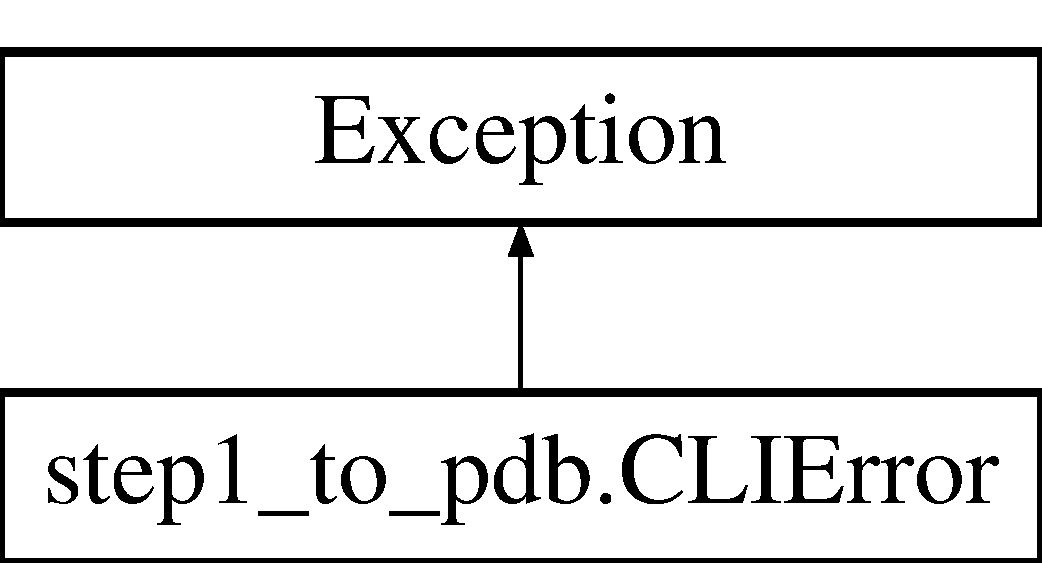
\includegraphics[height=2.000000cm]{classstep1__to__pdb_1_1_c_l_i_error}
\end{center}
\end{figure}
\subsection*{Public Member Functions}
\begin{DoxyCompactItemize}
\item 
def \hyperlink{classstep1__to__pdb_1_1_c_l_i_error_af7ef908bc07f68e5f79a620dde83dba0}{\-\_\-\-\_\-init\-\_\-\-\_\-}
\item 
def \hyperlink{classstep1__to__pdb_1_1_c_l_i_error_a75c25a11ea5c4ab13bc7970fc85e8487}{\-\_\-\-\_\-str\-\_\-\-\_\-}
\item 
def \hyperlink{classstep1__to__pdb_1_1_c_l_i_error_a5227949d447b7d28c3fec0983891c004}{\-\_\-\-\_\-unicode\-\_\-\-\_\-}
\end{DoxyCompactItemize}
\subsection*{Public Attributes}
\begin{DoxyCompactItemize}
\item 
\hyperlink{classstep1__to__pdb_1_1_c_l_i_error_adc73a367f4c49d59a08eb66d2d95dfc5}{msg}
\end{DoxyCompactItemize}


\subsection{Detailed Description}
Generic exception to raise and log different fatal errors. 



\subsection{Constructor \& Destructor Documentation}
\hypertarget{classstep1__to__pdb_1_1_c_l_i_error_af7ef908bc07f68e5f79a620dde83dba0}{\index{step1\-\_\-to\-\_\-pdb\-::\-C\-L\-I\-Error@{step1\-\_\-to\-\_\-pdb\-::\-C\-L\-I\-Error}!\-\_\-\-\_\-init\-\_\-\-\_\-@{\-\_\-\-\_\-init\-\_\-\-\_\-}}
\index{\-\_\-\-\_\-init\-\_\-\-\_\-@{\-\_\-\-\_\-init\-\_\-\-\_\-}!step1_to_pdb::CLIError@{step1\-\_\-to\-\_\-pdb\-::\-C\-L\-I\-Error}}
\subsubsection[{\-\_\-\-\_\-init\-\_\-\-\_\-}]{\setlength{\rightskip}{0pt plus 5cm}def step1\-\_\-to\-\_\-pdb.\-C\-L\-I\-Error.\-\_\-\-\_\-init\-\_\-\-\_\- (
\begin{DoxyParamCaption}
\item[{}]{self, }
\item[{}]{msg}
\end{DoxyParamCaption}
)}}\label{classstep1__to__pdb_1_1_c_l_i_error_af7ef908bc07f68e5f79a620dde83dba0}


\subsection{Member Function Documentation}
\hypertarget{classstep1__to__pdb_1_1_c_l_i_error_a75c25a11ea5c4ab13bc7970fc85e8487}{\index{step1\-\_\-to\-\_\-pdb\-::\-C\-L\-I\-Error@{step1\-\_\-to\-\_\-pdb\-::\-C\-L\-I\-Error}!\-\_\-\-\_\-str\-\_\-\-\_\-@{\-\_\-\-\_\-str\-\_\-\-\_\-}}
\index{\-\_\-\-\_\-str\-\_\-\-\_\-@{\-\_\-\-\_\-str\-\_\-\-\_\-}!step1_to_pdb::CLIError@{step1\-\_\-to\-\_\-pdb\-::\-C\-L\-I\-Error}}
\subsubsection[{\-\_\-\-\_\-str\-\_\-\-\_\-}]{\setlength{\rightskip}{0pt plus 5cm}def step1\-\_\-to\-\_\-pdb.\-C\-L\-I\-Error.\-\_\-\-\_\-str\-\_\-\-\_\- (
\begin{DoxyParamCaption}
\item[{}]{self}
\end{DoxyParamCaption}
)}}\label{classstep1__to__pdb_1_1_c_l_i_error_a75c25a11ea5c4ab13bc7970fc85e8487}
\hypertarget{classstep1__to__pdb_1_1_c_l_i_error_a5227949d447b7d28c3fec0983891c004}{\index{step1\-\_\-to\-\_\-pdb\-::\-C\-L\-I\-Error@{step1\-\_\-to\-\_\-pdb\-::\-C\-L\-I\-Error}!\-\_\-\-\_\-unicode\-\_\-\-\_\-@{\-\_\-\-\_\-unicode\-\_\-\-\_\-}}
\index{\-\_\-\-\_\-unicode\-\_\-\-\_\-@{\-\_\-\-\_\-unicode\-\_\-\-\_\-}!step1_to_pdb::CLIError@{step1\-\_\-to\-\_\-pdb\-::\-C\-L\-I\-Error}}
\subsubsection[{\-\_\-\-\_\-unicode\-\_\-\-\_\-}]{\setlength{\rightskip}{0pt plus 5cm}def step1\-\_\-to\-\_\-pdb.\-C\-L\-I\-Error.\-\_\-\-\_\-unicode\-\_\-\-\_\- (
\begin{DoxyParamCaption}
\item[{}]{self}
\end{DoxyParamCaption}
)}}\label{classstep1__to__pdb_1_1_c_l_i_error_a5227949d447b7d28c3fec0983891c004}


\subsection{Member Data Documentation}
\hypertarget{classstep1__to__pdb_1_1_c_l_i_error_adc73a367f4c49d59a08eb66d2d95dfc5}{\index{step1\-\_\-to\-\_\-pdb\-::\-C\-L\-I\-Error@{step1\-\_\-to\-\_\-pdb\-::\-C\-L\-I\-Error}!msg@{msg}}
\index{msg@{msg}!step1_to_pdb::CLIError@{step1\-\_\-to\-\_\-pdb\-::\-C\-L\-I\-Error}}
\subsubsection[{msg}]{\setlength{\rightskip}{0pt plus 5cm}step1\-\_\-to\-\_\-pdb.\-C\-L\-I\-Error.\-msg}}\label{classstep1__to__pdb_1_1_c_l_i_error_adc73a367f4c49d59a08eb66d2d95dfc5}


The documentation for this class was generated from the following file\-:\begin{DoxyCompactItemize}
\item 
src/scripts/mcce/\hyperlink{step1__to__pdb_8py}{step1\-\_\-to\-\_\-pdb.\-py}\end{DoxyCompactItemize}

\hypertarget{classarg82__conn_1_1_conf}{\section{arg82\-\_\-conn.\-Conf Class Reference}
\label{classarg82__conn_1_1_conf}\index{arg82\-\_\-conn.\-Conf@{arg82\-\_\-conn.\-Conf}}
}
Inheritance diagram for arg82\-\_\-conn.\-Conf\-:\begin{figure}[H]
\begin{center}
\leavevmode
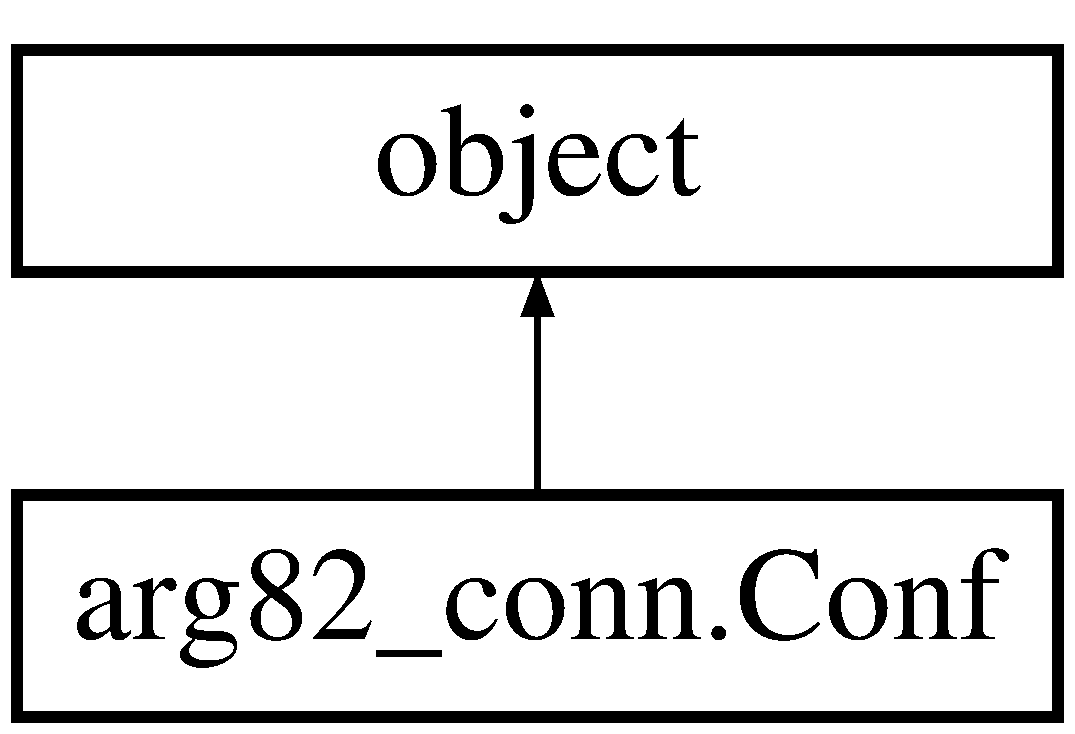
\includegraphics[height=2.000000cm]{classarg82__conn_1_1_conf}
\end{center}
\end{figure}
\subsection*{Public Member Functions}
\begin{DoxyCompactItemize}
\item 
def \hyperlink{classarg82__conn_1_1_conf_adaa69c48049cd99213ed89b9492482fc}{\-\_\-\-\_\-init\-\_\-\-\_\-}
\end{DoxyCompactItemize}
\subsection*{Public Attributes}
\begin{DoxyCompactItemize}
\item 
\hyperlink{classarg82__conn_1_1_conf_a5deba118eecc268ec28a4a6a50fb94e7}{conf\-Name}
\item 
\hyperlink{classarg82__conn_1_1_conf_a5697a79bbdd586706897f5b170bfe3eb}{occ}
\end{DoxyCompactItemize}


\subsection{Constructor \& Destructor Documentation}
\hypertarget{classarg82__conn_1_1_conf_adaa69c48049cd99213ed89b9492482fc}{\index{arg82\-\_\-conn\-::\-Conf@{arg82\-\_\-conn\-::\-Conf}!\-\_\-\-\_\-init\-\_\-\-\_\-@{\-\_\-\-\_\-init\-\_\-\-\_\-}}
\index{\-\_\-\-\_\-init\-\_\-\-\_\-@{\-\_\-\-\_\-init\-\_\-\-\_\-}!arg82_conn::Conf@{arg82\-\_\-conn\-::\-Conf}}
\subsubsection[{\-\_\-\-\_\-init\-\_\-\-\_\-}]{\setlength{\rightskip}{0pt plus 5cm}def arg82\-\_\-conn.\-Conf.\-\_\-\-\_\-init\-\_\-\-\_\- (
\begin{DoxyParamCaption}
\item[{}]{self}
\end{DoxyParamCaption}
)}}\label{classarg82__conn_1_1_conf_adaa69c48049cd99213ed89b9492482fc}


\subsection{Member Data Documentation}
\hypertarget{classarg82__conn_1_1_conf_a5deba118eecc268ec28a4a6a50fb94e7}{\index{arg82\-\_\-conn\-::\-Conf@{arg82\-\_\-conn\-::\-Conf}!conf\-Name@{conf\-Name}}
\index{conf\-Name@{conf\-Name}!arg82_conn::Conf@{arg82\-\_\-conn\-::\-Conf}}
\subsubsection[{conf\-Name}]{\setlength{\rightskip}{0pt plus 5cm}arg82\-\_\-conn.\-Conf.\-conf\-Name}}\label{classarg82__conn_1_1_conf_a5deba118eecc268ec28a4a6a50fb94e7}
\hypertarget{classarg82__conn_1_1_conf_a5697a79bbdd586706897f5b170bfe3eb}{\index{arg82\-\_\-conn\-::\-Conf@{arg82\-\_\-conn\-::\-Conf}!occ@{occ}}
\index{occ@{occ}!arg82_conn::Conf@{arg82\-\_\-conn\-::\-Conf}}
\subsubsection[{occ}]{\setlength{\rightskip}{0pt plus 5cm}arg82\-\_\-conn.\-Conf.\-occ}}\label{classarg82__conn_1_1_conf_a5697a79bbdd586706897f5b170bfe3eb}


The documentation for this class was generated from the following file\-:\begin{DoxyCompactItemize}
\item 
src/scripts/hb\-\_\-connection/\hyperlink{arg82__conn_8py}{arg82\-\_\-conn.\-py}\end{DoxyCompactItemize}

\hypertarget{classmocc_1_1_conf}{\section{mocc.\-Conf Class Reference}
\label{classmocc_1_1_conf}\index{mocc.\-Conf@{mocc.\-Conf}}
}


Conformer class.  


Inheritance diagram for mocc.\-Conf\-:\begin{figure}[H]
\begin{center}
\leavevmode
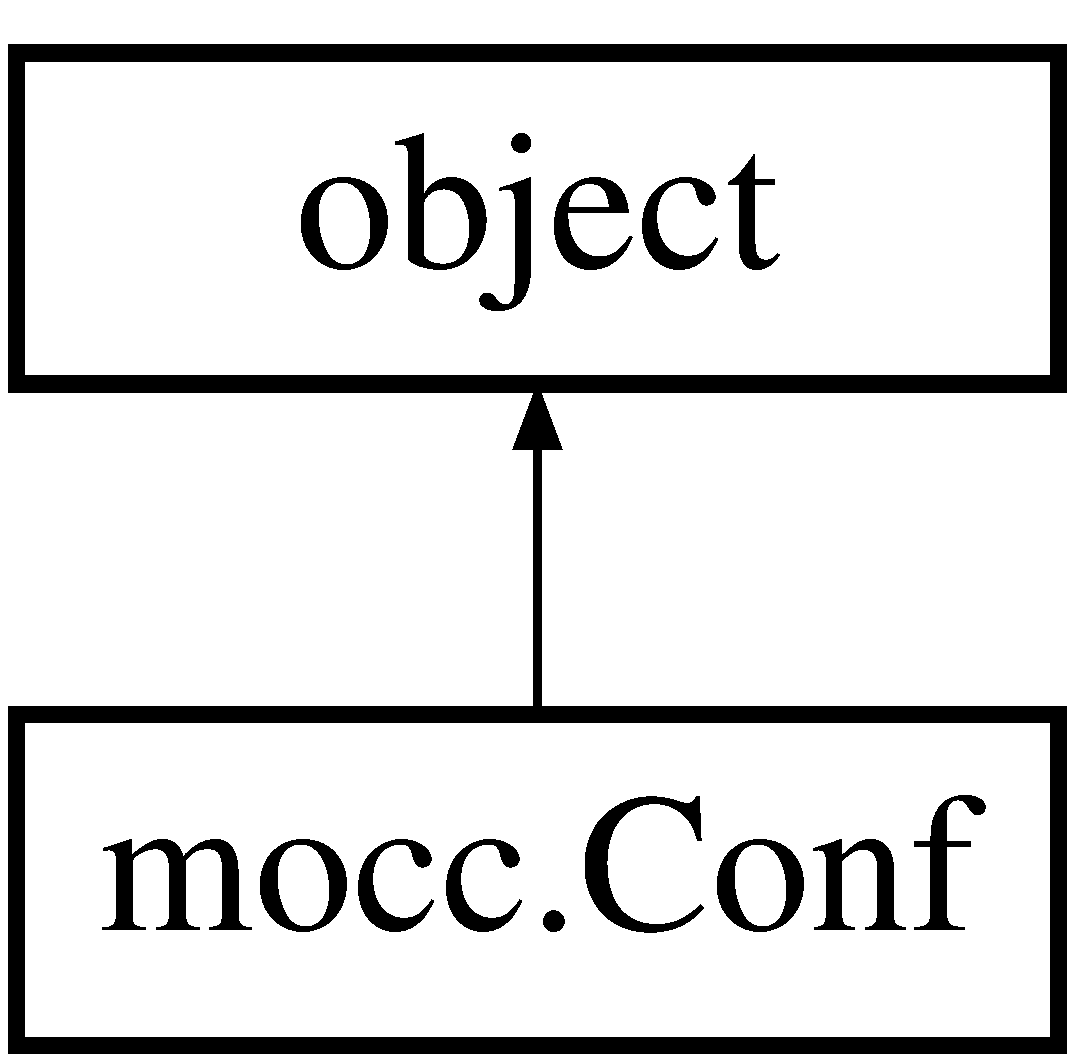
\includegraphics[height=2.000000cm]{classmocc_1_1_conf}
\end{center}
\end{figure}
\subsection*{Public Member Functions}
\begin{DoxyCompactItemize}
\item 
def \hyperlink{classmocc_1_1_conf_aa500603293a8484e5a5be6b8c464aea2}{\-\_\-\-\_\-init\-\_\-\-\_\-}
\item 
def \hyperlink{classmocc_1_1_conf_acd95b13da7989dcab1ae34694c4a1869}{load\-\_\-s2}
\begin{DoxyCompactList}\small\item\em Load the info of the conformer from a line in \char`\"{}step2\-\_\-out.\-pdb\char`\"{}. \end{DoxyCompactList}\item 
def \hyperlink{classmocc_1_1_conf_a70483b8650a6ea020699a2aeeeb8bc8b}{write\-\_\-pdb}
\begin{DoxyCompactList}\small\item\em Write the conformer to a pdb file. \end{DoxyCompactList}\end{DoxyCompactItemize}
\subsection*{Public Attributes}
\begin{DoxyCompactItemize}
\item 
\hyperlink{classmocc_1_1_conf_aca1ad7dd1cbd3016b49d0324cd215a6c}{confid}
\item 
\hyperlink{classmocc_1_1_conf_a502e54dae7949b03753996d86fa00ec3}{occ}
\item 
\hyperlink{classmocc_1_1_conf_afb6520f03e8170fa7f13806ad6960b1e}{resid}
\item 
\hyperlink{classmocc_1_1_conf_a4d4f705ae22c4a96a17a63cfa5dbc51d}{chainid}
\item 
\hyperlink{classmocc_1_1_conf_a9b80e40b5c8f4ee88bb5c3c0e8864055}{resseq}
\item 
\hyperlink{classmocc_1_1_conf_a1a614c66d33ebd31d4f1493c90ca5ff5}{x2}
\item 
\hyperlink{classmocc_1_1_conf_a1bd6811ef470dd12245b214c639c50d5}{s\-\_\-head}
\item 
\hyperlink{classmocc_1_1_conf_abe64fbfee389298b7ab826e203c3684b}{cor}
\end{DoxyCompactItemize}


\subsection{Detailed Description}
Conformer class. 

\subsection{Constructor \& Destructor Documentation}
\hypertarget{classmocc_1_1_conf_aa500603293a8484e5a5be6b8c464aea2}{\index{mocc\-::\-Conf@{mocc\-::\-Conf}!\-\_\-\-\_\-init\-\_\-\-\_\-@{\-\_\-\-\_\-init\-\_\-\-\_\-}}
\index{\-\_\-\-\_\-init\-\_\-\-\_\-@{\-\_\-\-\_\-init\-\_\-\-\_\-}!mocc::Conf@{mocc\-::\-Conf}}
\subsubsection[{\-\_\-\-\_\-init\-\_\-\-\_\-}]{\setlength{\rightskip}{0pt plus 5cm}def mocc.\-Conf.\-\_\-\-\_\-init\-\_\-\-\_\- (
\begin{DoxyParamCaption}
\item[{}]{self, }
\item[{}]{f\-\_\-line, }
\item[{}]{t\-\_\-col}
\end{DoxyParamCaption}
)}}\label{classmocc_1_1_conf_aa500603293a8484e5a5be6b8c464aea2}


\subsection{Member Function Documentation}
\hypertarget{classmocc_1_1_conf_acd95b13da7989dcab1ae34694c4a1869}{\index{mocc\-::\-Conf@{mocc\-::\-Conf}!load\-\_\-s2@{load\-\_\-s2}}
\index{load\-\_\-s2@{load\-\_\-s2}!mocc::Conf@{mocc\-::\-Conf}}
\subsubsection[{load\-\_\-s2}]{\setlength{\rightskip}{0pt plus 5cm}def mocc.\-Conf.\-load\-\_\-s2 (
\begin{DoxyParamCaption}
\item[{}]{self, }
\item[{}]{s\-\_\-line}
\end{DoxyParamCaption}
)}}\label{classmocc_1_1_conf_acd95b13da7989dcab1ae34694c4a1869}


Load the info of the conformer from a line in \char`\"{}step2\-\_\-out.\-pdb\char`\"{}. 

One atom of the conformer is loaded. \hypertarget{classmocc_1_1_conf_a70483b8650a6ea020699a2aeeeb8bc8b}{\index{mocc\-::\-Conf@{mocc\-::\-Conf}!write\-\_\-pdb@{write\-\_\-pdb}}
\index{write\-\_\-pdb@{write\-\_\-pdb}!mocc::Conf@{mocc\-::\-Conf}}
\subsubsection[{write\-\_\-pdb}]{\setlength{\rightskip}{0pt plus 5cm}def mocc.\-Conf.\-write\-\_\-pdb (
\begin{DoxyParamCaption}
\item[{}]{self, }
\item[{}]{fp}
\end{DoxyParamCaption}
)}}\label{classmocc_1_1_conf_a70483b8650a6ea020699a2aeeeb8bc8b}


Write the conformer to a pdb file. 

All the atoms of this conformer need to be written. 

\subsection{Member Data Documentation}
\hypertarget{classmocc_1_1_conf_a4d4f705ae22c4a96a17a63cfa5dbc51d}{\index{mocc\-::\-Conf@{mocc\-::\-Conf}!chainid@{chainid}}
\index{chainid@{chainid}!mocc::Conf@{mocc\-::\-Conf}}
\subsubsection[{chainid}]{\setlength{\rightskip}{0pt plus 5cm}mocc.\-Conf.\-chainid}}\label{classmocc_1_1_conf_a4d4f705ae22c4a96a17a63cfa5dbc51d}
\hypertarget{classmocc_1_1_conf_aca1ad7dd1cbd3016b49d0324cd215a6c}{\index{mocc\-::\-Conf@{mocc\-::\-Conf}!confid@{confid}}
\index{confid@{confid}!mocc::Conf@{mocc\-::\-Conf}}
\subsubsection[{confid}]{\setlength{\rightskip}{0pt plus 5cm}mocc.\-Conf.\-confid}}\label{classmocc_1_1_conf_aca1ad7dd1cbd3016b49d0324cd215a6c}
\hypertarget{classmocc_1_1_conf_abe64fbfee389298b7ab826e203c3684b}{\index{mocc\-::\-Conf@{mocc\-::\-Conf}!cor@{cor}}
\index{cor@{cor}!mocc::Conf@{mocc\-::\-Conf}}
\subsubsection[{cor}]{\setlength{\rightskip}{0pt plus 5cm}mocc.\-Conf.\-cor}}\label{classmocc_1_1_conf_abe64fbfee389298b7ab826e203c3684b}
\hypertarget{classmocc_1_1_conf_a502e54dae7949b03753996d86fa00ec3}{\index{mocc\-::\-Conf@{mocc\-::\-Conf}!occ@{occ}}
\index{occ@{occ}!mocc::Conf@{mocc\-::\-Conf}}
\subsubsection[{occ}]{\setlength{\rightskip}{0pt plus 5cm}mocc.\-Conf.\-occ}}\label{classmocc_1_1_conf_a502e54dae7949b03753996d86fa00ec3}
\hypertarget{classmocc_1_1_conf_afb6520f03e8170fa7f13806ad6960b1e}{\index{mocc\-::\-Conf@{mocc\-::\-Conf}!resid@{resid}}
\index{resid@{resid}!mocc::Conf@{mocc\-::\-Conf}}
\subsubsection[{resid}]{\setlength{\rightskip}{0pt plus 5cm}mocc.\-Conf.\-resid}}\label{classmocc_1_1_conf_afb6520f03e8170fa7f13806ad6960b1e}
\hypertarget{classmocc_1_1_conf_a9b80e40b5c8f4ee88bb5c3c0e8864055}{\index{mocc\-::\-Conf@{mocc\-::\-Conf}!resseq@{resseq}}
\index{resseq@{resseq}!mocc::Conf@{mocc\-::\-Conf}}
\subsubsection[{resseq}]{\setlength{\rightskip}{0pt plus 5cm}mocc.\-Conf.\-resseq}}\label{classmocc_1_1_conf_a9b80e40b5c8f4ee88bb5c3c0e8864055}
\hypertarget{classmocc_1_1_conf_a1bd6811ef470dd12245b214c639c50d5}{\index{mocc\-::\-Conf@{mocc\-::\-Conf}!s\-\_\-head@{s\-\_\-head}}
\index{s\-\_\-head@{s\-\_\-head}!mocc::Conf@{mocc\-::\-Conf}}
\subsubsection[{s\-\_\-head}]{\setlength{\rightskip}{0pt plus 5cm}mocc.\-Conf.\-s\-\_\-head}}\label{classmocc_1_1_conf_a1bd6811ef470dd12245b214c639c50d5}
\hypertarget{classmocc_1_1_conf_a1a614c66d33ebd31d4f1493c90ca5ff5}{\index{mocc\-::\-Conf@{mocc\-::\-Conf}!x2@{x2}}
\index{x2@{x2}!mocc::Conf@{mocc\-::\-Conf}}
\subsubsection[{x2}]{\setlength{\rightskip}{0pt plus 5cm}mocc.\-Conf.\-x2}}\label{classmocc_1_1_conf_a1a614c66d33ebd31d4f1493c90ca5ff5}


The documentation for this class was generated from the following file\-:\begin{DoxyCompactItemize}
\item 
src/scripts/mcce/\hyperlink{mocc_8py}{mocc.\-py}\end{DoxyCompactItemize}

\hypertarget{classoccupied__confs_1_1_conf}{\section{occupied\-\_\-confs.\-Conf Class Reference}
\label{classoccupied__confs_1_1_conf}\index{occupied\-\_\-confs.\-Conf@{occupied\-\_\-confs.\-Conf}}
}
Inheritance diagram for occupied\-\_\-confs.\-Conf\-:\begin{figure}[H]
\begin{center}
\leavevmode
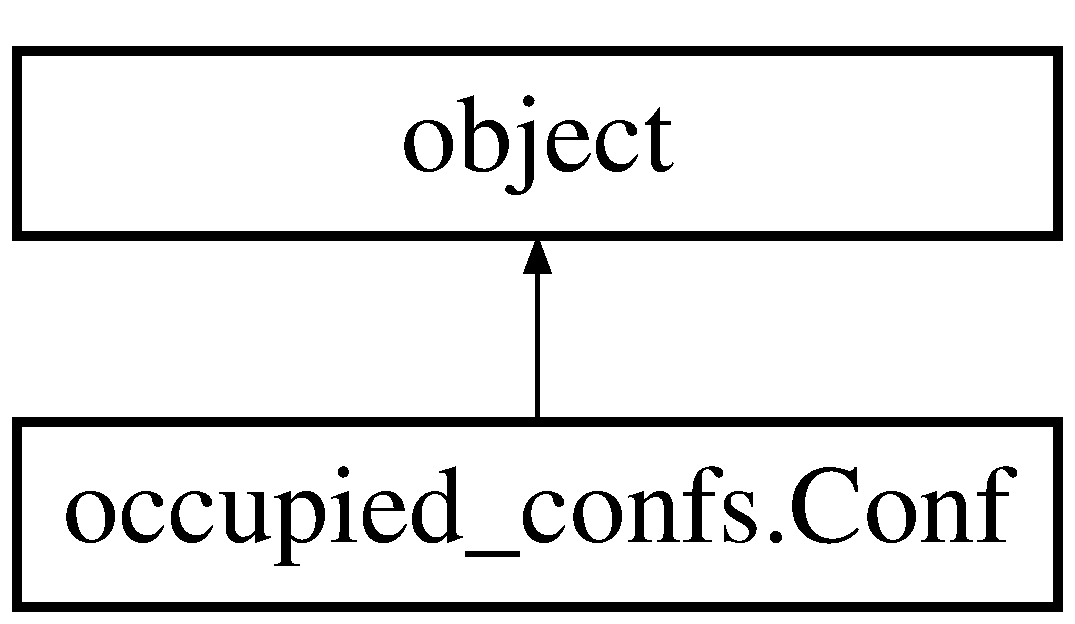
\includegraphics[height=2.000000cm]{classoccupied__confs_1_1_conf}
\end{center}
\end{figure}
\subsection*{Public Member Functions}
\begin{DoxyCompactItemize}
\item 
def \hyperlink{classoccupied__confs_1_1_conf_aa0dd7bf79293835ed9e9049b4096d5df}{\-\_\-\-\_\-init\-\_\-\-\_\-}
\item 
def \hyperlink{classoccupied__confs_1_1_conf_a86bd2eeb27506e2b4f3558a3965c9830}{\-\_\-\-\_\-str\-\_\-\-\_\-}
\item 
def \hyperlink{classoccupied__confs_1_1_conf_a3d672e0b7ba077097cbb121a5511fc1c}{is\-Dummy}
\item 
def \hyperlink{classoccupied__confs_1_1_conf_a29f61ef9aeb27bbd84df3cb668b46d4c}{read\-\_\-fort38\-\_\-line}
\item 
def \hyperlink{classoccupied__confs_1_1_conf_a841115a333f8d567defc2b67603ca37b}{read\-\_\-head3\-\_\-line}
\end{DoxyCompactItemize}
\subsection*{Public Attributes}
\begin{DoxyCompactItemize}
\item 
\hyperlink{classoccupied__confs_1_1_conf_a13949303b665dcbe679ee6e7bc022d8f}{conf\-Name}
\item 
\hyperlink{classoccupied__confs_1_1_conf_a797d50d931016f337df10b3d813caea3}{occ}
\item 
\hyperlink{classoccupied__confs_1_1_conf_a97ff8bf981ee6cfc298743680892051e}{Em0}
\item 
\hyperlink{classoccupied__confs_1_1_conf_acce23ba752fb707934705e2388544cbc}{p\-Ka0}
\item 
\hyperlink{classoccupied__confs_1_1_conf_aa887cabafc23bbe447bc3d91155589ec}{ne}
\item 
\hyperlink{classoccupied__confs_1_1_conf_a835a97d72341cd881b12d52e9d651b09}{n\-H}
\item 
\hyperlink{classoccupied__confs_1_1_conf_ac5e8f69fab016810e30c0189140539f0}{vdw0}
\item 
\hyperlink{classoccupied__confs_1_1_conf_a959ce58c489f1b8a8bb9326af6e0b23b}{vdw1}
\item 
\hyperlink{classoccupied__confs_1_1_conf_ae2c305a0232855e7bd218be00667fb5a}{tors}
\item 
\hyperlink{classoccupied__confs_1_1_conf_a668d3ddba815ed7b3b6b98f88fa7291c}{epol}
\item 
\hyperlink{classoccupied__confs_1_1_conf_ac272b12f782bc678d77918617f6556ce}{dsolv}
\item 
\hyperlink{classoccupied__confs_1_1_conf_a7bbb6bae26eaf92f7c8c6d886c7f36e8}{extra}
\item 
\hyperlink{classoccupied__confs_1_1_conf_ad829e213e264e618aabce225db742550}{total\-Self}
\item 
\hyperlink{classoccupied__confs_1_1_conf_aab1f60df9bbea17a434edaf55153cec2}{mfe\-Sum}
\end{DoxyCompactItemize}
\subsection*{Static Public Attributes}
\begin{DoxyCompactItemize}
\item 
float \hyperlink{classoccupied__confs_1_1_conf_a6edc3ff9b93e79bce68057ef9a83dc86}{P\-H\-\_\-\-N\-O\-W} = 7.\-0
\end{DoxyCompactItemize}


\subsection{Constructor \& Destructor Documentation}
\hypertarget{classoccupied__confs_1_1_conf_aa0dd7bf79293835ed9e9049b4096d5df}{\index{occupied\-\_\-confs\-::\-Conf@{occupied\-\_\-confs\-::\-Conf}!\-\_\-\-\_\-init\-\_\-\-\_\-@{\-\_\-\-\_\-init\-\_\-\-\_\-}}
\index{\-\_\-\-\_\-init\-\_\-\-\_\-@{\-\_\-\-\_\-init\-\_\-\-\_\-}!occupied_confs::Conf@{occupied\-\_\-confs\-::\-Conf}}
\subsubsection[{\-\_\-\-\_\-init\-\_\-\-\_\-}]{\setlength{\rightskip}{0pt plus 5cm}def occupied\-\_\-confs.\-Conf.\-\_\-\-\_\-init\-\_\-\-\_\- (
\begin{DoxyParamCaption}
\item[{}]{self}
\end{DoxyParamCaption}
)}}\label{classoccupied__confs_1_1_conf_aa0dd7bf79293835ed9e9049b4096d5df}


\subsection{Member Function Documentation}
\hypertarget{classoccupied__confs_1_1_conf_a86bd2eeb27506e2b4f3558a3965c9830}{\index{occupied\-\_\-confs\-::\-Conf@{occupied\-\_\-confs\-::\-Conf}!\-\_\-\-\_\-str\-\_\-\-\_\-@{\-\_\-\-\_\-str\-\_\-\-\_\-}}
\index{\-\_\-\-\_\-str\-\_\-\-\_\-@{\-\_\-\-\_\-str\-\_\-\-\_\-}!occupied_confs::Conf@{occupied\-\_\-confs\-::\-Conf}}
\subsubsection[{\-\_\-\-\_\-str\-\_\-\-\_\-}]{\setlength{\rightskip}{0pt plus 5cm}def occupied\-\_\-confs.\-Conf.\-\_\-\-\_\-str\-\_\-\-\_\- (
\begin{DoxyParamCaption}
\item[{}]{self}
\end{DoxyParamCaption}
)}}\label{classoccupied__confs_1_1_conf_a86bd2eeb27506e2b4f3558a3965c9830}
\hypertarget{classoccupied__confs_1_1_conf_a3d672e0b7ba077097cbb121a5511fc1c}{\index{occupied\-\_\-confs\-::\-Conf@{occupied\-\_\-confs\-::\-Conf}!is\-Dummy@{is\-Dummy}}
\index{is\-Dummy@{is\-Dummy}!occupied_confs::Conf@{occupied\-\_\-confs\-::\-Conf}}
\subsubsection[{is\-Dummy}]{\setlength{\rightskip}{0pt plus 5cm}def occupied\-\_\-confs.\-Conf.\-is\-Dummy (
\begin{DoxyParamCaption}
\item[{}]{self}
\end{DoxyParamCaption}
)}}\label{classoccupied__confs_1_1_conf_a3d672e0b7ba077097cbb121a5511fc1c}
\hypertarget{classoccupied__confs_1_1_conf_a29f61ef9aeb27bbd84df3cb668b46d4c}{\index{occupied\-\_\-confs\-::\-Conf@{occupied\-\_\-confs\-::\-Conf}!read\-\_\-fort38\-\_\-line@{read\-\_\-fort38\-\_\-line}}
\index{read\-\_\-fort38\-\_\-line@{read\-\_\-fort38\-\_\-line}!occupied_confs::Conf@{occupied\-\_\-confs\-::\-Conf}}
\subsubsection[{read\-\_\-fort38\-\_\-line}]{\setlength{\rightskip}{0pt plus 5cm}def occupied\-\_\-confs.\-Conf.\-read\-\_\-fort38\-\_\-line (
\begin{DoxyParamCaption}
\item[{}]{self, }
\item[{}]{line}
\end{DoxyParamCaption}
)}}\label{classoccupied__confs_1_1_conf_a29f61ef9aeb27bbd84df3cb668b46d4c}
\hypertarget{classoccupied__confs_1_1_conf_a841115a333f8d567defc2b67603ca37b}{\index{occupied\-\_\-confs\-::\-Conf@{occupied\-\_\-confs\-::\-Conf}!read\-\_\-head3\-\_\-line@{read\-\_\-head3\-\_\-line}}
\index{read\-\_\-head3\-\_\-line@{read\-\_\-head3\-\_\-line}!occupied_confs::Conf@{occupied\-\_\-confs\-::\-Conf}}
\subsubsection[{read\-\_\-head3\-\_\-line}]{\setlength{\rightskip}{0pt plus 5cm}def occupied\-\_\-confs.\-Conf.\-read\-\_\-head3\-\_\-line (
\begin{DoxyParamCaption}
\item[{}]{self, }
\item[{}]{line}
\end{DoxyParamCaption}
)}}\label{classoccupied__confs_1_1_conf_a841115a333f8d567defc2b67603ca37b}


\subsection{Member Data Documentation}
\hypertarget{classoccupied__confs_1_1_conf_a13949303b665dcbe679ee6e7bc022d8f}{\index{occupied\-\_\-confs\-::\-Conf@{occupied\-\_\-confs\-::\-Conf}!conf\-Name@{conf\-Name}}
\index{conf\-Name@{conf\-Name}!occupied_confs::Conf@{occupied\-\_\-confs\-::\-Conf}}
\subsubsection[{conf\-Name}]{\setlength{\rightskip}{0pt plus 5cm}occupied\-\_\-confs.\-Conf.\-conf\-Name}}\label{classoccupied__confs_1_1_conf_a13949303b665dcbe679ee6e7bc022d8f}
\hypertarget{classoccupied__confs_1_1_conf_ac272b12f782bc678d77918617f6556ce}{\index{occupied\-\_\-confs\-::\-Conf@{occupied\-\_\-confs\-::\-Conf}!dsolv@{dsolv}}
\index{dsolv@{dsolv}!occupied_confs::Conf@{occupied\-\_\-confs\-::\-Conf}}
\subsubsection[{dsolv}]{\setlength{\rightskip}{0pt plus 5cm}occupied\-\_\-confs.\-Conf.\-dsolv}}\label{classoccupied__confs_1_1_conf_ac272b12f782bc678d77918617f6556ce}
\hypertarget{classoccupied__confs_1_1_conf_a97ff8bf981ee6cfc298743680892051e}{\index{occupied\-\_\-confs\-::\-Conf@{occupied\-\_\-confs\-::\-Conf}!Em0@{Em0}}
\index{Em0@{Em0}!occupied_confs::Conf@{occupied\-\_\-confs\-::\-Conf}}
\subsubsection[{Em0}]{\setlength{\rightskip}{0pt plus 5cm}occupied\-\_\-confs.\-Conf.\-Em0}}\label{classoccupied__confs_1_1_conf_a97ff8bf981ee6cfc298743680892051e}
\hypertarget{classoccupied__confs_1_1_conf_a668d3ddba815ed7b3b6b98f88fa7291c}{\index{occupied\-\_\-confs\-::\-Conf@{occupied\-\_\-confs\-::\-Conf}!epol@{epol}}
\index{epol@{epol}!occupied_confs::Conf@{occupied\-\_\-confs\-::\-Conf}}
\subsubsection[{epol}]{\setlength{\rightskip}{0pt plus 5cm}occupied\-\_\-confs.\-Conf.\-epol}}\label{classoccupied__confs_1_1_conf_a668d3ddba815ed7b3b6b98f88fa7291c}
\hypertarget{classoccupied__confs_1_1_conf_a7bbb6bae26eaf92f7c8c6d886c7f36e8}{\index{occupied\-\_\-confs\-::\-Conf@{occupied\-\_\-confs\-::\-Conf}!extra@{extra}}
\index{extra@{extra}!occupied_confs::Conf@{occupied\-\_\-confs\-::\-Conf}}
\subsubsection[{extra}]{\setlength{\rightskip}{0pt plus 5cm}occupied\-\_\-confs.\-Conf.\-extra}}\label{classoccupied__confs_1_1_conf_a7bbb6bae26eaf92f7c8c6d886c7f36e8}
\hypertarget{classoccupied__confs_1_1_conf_aab1f60df9bbea17a434edaf55153cec2}{\index{occupied\-\_\-confs\-::\-Conf@{occupied\-\_\-confs\-::\-Conf}!mfe\-Sum@{mfe\-Sum}}
\index{mfe\-Sum@{mfe\-Sum}!occupied_confs::Conf@{occupied\-\_\-confs\-::\-Conf}}
\subsubsection[{mfe\-Sum}]{\setlength{\rightskip}{0pt plus 5cm}occupied\-\_\-confs.\-Conf.\-mfe\-Sum}}\label{classoccupied__confs_1_1_conf_aab1f60df9bbea17a434edaf55153cec2}
\hypertarget{classoccupied__confs_1_1_conf_aa887cabafc23bbe447bc3d91155589ec}{\index{occupied\-\_\-confs\-::\-Conf@{occupied\-\_\-confs\-::\-Conf}!ne@{ne}}
\index{ne@{ne}!occupied_confs::Conf@{occupied\-\_\-confs\-::\-Conf}}
\subsubsection[{ne}]{\setlength{\rightskip}{0pt plus 5cm}occupied\-\_\-confs.\-Conf.\-ne}}\label{classoccupied__confs_1_1_conf_aa887cabafc23bbe447bc3d91155589ec}
\hypertarget{classoccupied__confs_1_1_conf_a835a97d72341cd881b12d52e9d651b09}{\index{occupied\-\_\-confs\-::\-Conf@{occupied\-\_\-confs\-::\-Conf}!n\-H@{n\-H}}
\index{n\-H@{n\-H}!occupied_confs::Conf@{occupied\-\_\-confs\-::\-Conf}}
\subsubsection[{n\-H}]{\setlength{\rightskip}{0pt plus 5cm}occupied\-\_\-confs.\-Conf.\-n\-H}}\label{classoccupied__confs_1_1_conf_a835a97d72341cd881b12d52e9d651b09}
\hypertarget{classoccupied__confs_1_1_conf_a797d50d931016f337df10b3d813caea3}{\index{occupied\-\_\-confs\-::\-Conf@{occupied\-\_\-confs\-::\-Conf}!occ@{occ}}
\index{occ@{occ}!occupied_confs::Conf@{occupied\-\_\-confs\-::\-Conf}}
\subsubsection[{occ}]{\setlength{\rightskip}{0pt plus 5cm}occupied\-\_\-confs.\-Conf.\-occ}}\label{classoccupied__confs_1_1_conf_a797d50d931016f337df10b3d813caea3}
\hypertarget{classoccupied__confs_1_1_conf_a6edc3ff9b93e79bce68057ef9a83dc86}{\index{occupied\-\_\-confs\-::\-Conf@{occupied\-\_\-confs\-::\-Conf}!P\-H\-\_\-\-N\-O\-W@{P\-H\-\_\-\-N\-O\-W}}
\index{P\-H\-\_\-\-N\-O\-W@{P\-H\-\_\-\-N\-O\-W}!occupied_confs::Conf@{occupied\-\_\-confs\-::\-Conf}}
\subsubsection[{P\-H\-\_\-\-N\-O\-W}]{\setlength{\rightskip}{0pt plus 5cm}float occupied\-\_\-confs.\-Conf.\-P\-H\-\_\-\-N\-O\-W = 7.\-0\hspace{0.3cm}{\ttfamily [static]}}}\label{classoccupied__confs_1_1_conf_a6edc3ff9b93e79bce68057ef9a83dc86}
\hypertarget{classoccupied__confs_1_1_conf_acce23ba752fb707934705e2388544cbc}{\index{occupied\-\_\-confs\-::\-Conf@{occupied\-\_\-confs\-::\-Conf}!p\-Ka0@{p\-Ka0}}
\index{p\-Ka0@{p\-Ka0}!occupied_confs::Conf@{occupied\-\_\-confs\-::\-Conf}}
\subsubsection[{p\-Ka0}]{\setlength{\rightskip}{0pt plus 5cm}occupied\-\_\-confs.\-Conf.\-p\-Ka0}}\label{classoccupied__confs_1_1_conf_acce23ba752fb707934705e2388544cbc}
\hypertarget{classoccupied__confs_1_1_conf_ae2c305a0232855e7bd218be00667fb5a}{\index{occupied\-\_\-confs\-::\-Conf@{occupied\-\_\-confs\-::\-Conf}!tors@{tors}}
\index{tors@{tors}!occupied_confs::Conf@{occupied\-\_\-confs\-::\-Conf}}
\subsubsection[{tors}]{\setlength{\rightskip}{0pt plus 5cm}occupied\-\_\-confs.\-Conf.\-tors}}\label{classoccupied__confs_1_1_conf_ae2c305a0232855e7bd218be00667fb5a}
\hypertarget{classoccupied__confs_1_1_conf_ad829e213e264e618aabce225db742550}{\index{occupied\-\_\-confs\-::\-Conf@{occupied\-\_\-confs\-::\-Conf}!total\-Self@{total\-Self}}
\index{total\-Self@{total\-Self}!occupied_confs::Conf@{occupied\-\_\-confs\-::\-Conf}}
\subsubsection[{total\-Self}]{\setlength{\rightskip}{0pt plus 5cm}occupied\-\_\-confs.\-Conf.\-total\-Self}}\label{classoccupied__confs_1_1_conf_ad829e213e264e618aabce225db742550}
\hypertarget{classoccupied__confs_1_1_conf_ac5e8f69fab016810e30c0189140539f0}{\index{occupied\-\_\-confs\-::\-Conf@{occupied\-\_\-confs\-::\-Conf}!vdw0@{vdw0}}
\index{vdw0@{vdw0}!occupied_confs::Conf@{occupied\-\_\-confs\-::\-Conf}}
\subsubsection[{vdw0}]{\setlength{\rightskip}{0pt plus 5cm}occupied\-\_\-confs.\-Conf.\-vdw0}}\label{classoccupied__confs_1_1_conf_ac5e8f69fab016810e30c0189140539f0}
\hypertarget{classoccupied__confs_1_1_conf_a959ce58c489f1b8a8bb9326af6e0b23b}{\index{occupied\-\_\-confs\-::\-Conf@{occupied\-\_\-confs\-::\-Conf}!vdw1@{vdw1}}
\index{vdw1@{vdw1}!occupied_confs::Conf@{occupied\-\_\-confs\-::\-Conf}}
\subsubsection[{vdw1}]{\setlength{\rightskip}{0pt plus 5cm}occupied\-\_\-confs.\-Conf.\-vdw1}}\label{classoccupied__confs_1_1_conf_a959ce58c489f1b8a8bb9326af6e0b23b}


The documentation for this class was generated from the following file\-:\begin{DoxyCompactItemize}
\item 
src/scripts/old/\hyperlink{occupied__confs_8py}{occupied\-\_\-confs.\-py}\end{DoxyCompactItemize}

\hypertarget{classsetuptest_1_1_conf}{\section{setuptest.\-Conf Class Reference}
\label{classsetuptest_1_1_conf}\index{setuptest.\-Conf@{setuptest.\-Conf}}
}
Inheritance diagram for setuptest.\-Conf\-:\begin{figure}[H]
\begin{center}
\leavevmode
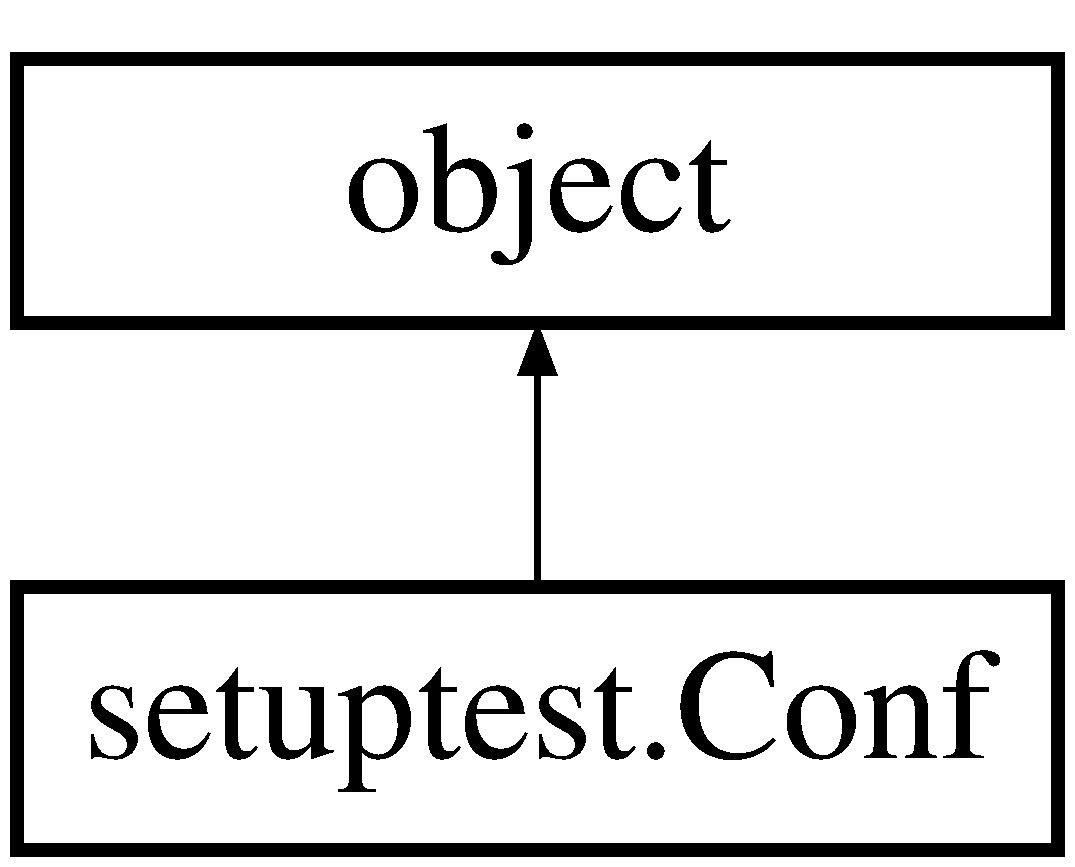
\includegraphics[height=2.000000cm]{classsetuptest_1_1_conf}
\end{center}
\end{figure}
\subsection*{Public Member Functions}
\begin{DoxyCompactItemize}
\item 
def \hyperlink{classsetuptest_1_1_conf_a48fc1bcd9f7cbd067e879a36a9f4c35f}{\-\_\-\-\_\-init\-\_\-\-\_\-}
\item 
def \hyperlink{classsetuptest_1_1_conf_ab7499595f3507bae83ffdbdba335f0c6}{init\-From\-Line}
\end{DoxyCompactItemize}
\subsection*{Public Attributes}
\begin{DoxyCompactItemize}
\item 
\hyperlink{classsetuptest_1_1_conf_a452e948db88329edca628da42df7efa4}{name}
\item 
\hyperlink{classsetuptest_1_1_conf_a11548ab44fdc3b46377a905ac60407c4}{flag}
\item 
\hyperlink{classsetuptest_1_1_conf_a986003b2244aef6dfb9f691bda3719e5}{E\-\_\-self}
\item 
\hyperlink{classsetuptest_1_1_conf_aa03d2c623ea2025ce30627696a2c89dd}{mcs}
\item 
\hyperlink{classsetuptest_1_1_conf_aa0a737a680ff2ce3e2ecd1a1f2611dd0}{occ}
\item 
\hyperlink{classsetuptest_1_1_conf_adb6b4cbd0a0cefeaa6618ed939240d47}{sgm}
\end{DoxyCompactItemize}


\subsection{Constructor \& Destructor Documentation}
\hypertarget{classsetuptest_1_1_conf_a48fc1bcd9f7cbd067e879a36a9f4c35f}{\index{setuptest\-::\-Conf@{setuptest\-::\-Conf}!\-\_\-\-\_\-init\-\_\-\-\_\-@{\-\_\-\-\_\-init\-\_\-\-\_\-}}
\index{\-\_\-\-\_\-init\-\_\-\-\_\-@{\-\_\-\-\_\-init\-\_\-\-\_\-}!setuptest::Conf@{setuptest\-::\-Conf}}
\subsubsection[{\-\_\-\-\_\-init\-\_\-\-\_\-}]{\setlength{\rightskip}{0pt plus 5cm}def setuptest.\-Conf.\-\_\-\-\_\-init\-\_\-\-\_\- (
\begin{DoxyParamCaption}
\item[{}]{self}
\end{DoxyParamCaption}
)}}\label{classsetuptest_1_1_conf_a48fc1bcd9f7cbd067e879a36a9f4c35f}


\subsection{Member Function Documentation}
\hypertarget{classsetuptest_1_1_conf_ab7499595f3507bae83ffdbdba335f0c6}{\index{setuptest\-::\-Conf@{setuptest\-::\-Conf}!init\-From\-Line@{init\-From\-Line}}
\index{init\-From\-Line@{init\-From\-Line}!setuptest::Conf@{setuptest\-::\-Conf}}
\subsubsection[{init\-From\-Line}]{\setlength{\rightskip}{0pt plus 5cm}def setuptest.\-Conf.\-init\-From\-Line (
\begin{DoxyParamCaption}
\item[{}]{self, }
\item[{}]{line}
\end{DoxyParamCaption}
)}}\label{classsetuptest_1_1_conf_ab7499595f3507bae83ffdbdba335f0c6}


\subsection{Member Data Documentation}
\hypertarget{classsetuptest_1_1_conf_a986003b2244aef6dfb9f691bda3719e5}{\index{setuptest\-::\-Conf@{setuptest\-::\-Conf}!E\-\_\-self@{E\-\_\-self}}
\index{E\-\_\-self@{E\-\_\-self}!setuptest::Conf@{setuptest\-::\-Conf}}
\subsubsection[{E\-\_\-self}]{\setlength{\rightskip}{0pt plus 5cm}setuptest.\-Conf.\-E\-\_\-self}}\label{classsetuptest_1_1_conf_a986003b2244aef6dfb9f691bda3719e5}
\hypertarget{classsetuptest_1_1_conf_a11548ab44fdc3b46377a905ac60407c4}{\index{setuptest\-::\-Conf@{setuptest\-::\-Conf}!flag@{flag}}
\index{flag@{flag}!setuptest::Conf@{setuptest\-::\-Conf}}
\subsubsection[{flag}]{\setlength{\rightskip}{0pt plus 5cm}setuptest.\-Conf.\-flag}}\label{classsetuptest_1_1_conf_a11548ab44fdc3b46377a905ac60407c4}
\hypertarget{classsetuptest_1_1_conf_aa03d2c623ea2025ce30627696a2c89dd}{\index{setuptest\-::\-Conf@{setuptest\-::\-Conf}!mcs@{mcs}}
\index{mcs@{mcs}!setuptest::Conf@{setuptest\-::\-Conf}}
\subsubsection[{mcs}]{\setlength{\rightskip}{0pt plus 5cm}setuptest.\-Conf.\-mcs}}\label{classsetuptest_1_1_conf_aa03d2c623ea2025ce30627696a2c89dd}
\hypertarget{classsetuptest_1_1_conf_a452e948db88329edca628da42df7efa4}{\index{setuptest\-::\-Conf@{setuptest\-::\-Conf}!name@{name}}
\index{name@{name}!setuptest::Conf@{setuptest\-::\-Conf}}
\subsubsection[{name}]{\setlength{\rightskip}{0pt plus 5cm}setuptest.\-Conf.\-name}}\label{classsetuptest_1_1_conf_a452e948db88329edca628da42df7efa4}
\hypertarget{classsetuptest_1_1_conf_aa0a737a680ff2ce3e2ecd1a1f2611dd0}{\index{setuptest\-::\-Conf@{setuptest\-::\-Conf}!occ@{occ}}
\index{occ@{occ}!setuptest::Conf@{setuptest\-::\-Conf}}
\subsubsection[{occ}]{\setlength{\rightskip}{0pt plus 5cm}setuptest.\-Conf.\-occ}}\label{classsetuptest_1_1_conf_aa0a737a680ff2ce3e2ecd1a1f2611dd0}
\hypertarget{classsetuptest_1_1_conf_adb6b4cbd0a0cefeaa6618ed939240d47}{\index{setuptest\-::\-Conf@{setuptest\-::\-Conf}!sgm@{sgm}}
\index{sgm@{sgm}!setuptest::Conf@{setuptest\-::\-Conf}}
\subsubsection[{sgm}]{\setlength{\rightskip}{0pt plus 5cm}setuptest.\-Conf.\-sgm}}\label{classsetuptest_1_1_conf_adb6b4cbd0a0cefeaa6618ed939240d47}


The documentation for this class was generated from the following file\-:\begin{DoxyCompactItemize}
\item 
src/scripts/old/\hyperlink{setuptest_8py}{setuptest.\-py}\end{DoxyCompactItemize}

\hypertarget{classcomp__occ_1_1_conf}{\section{comp\-\_\-occ.\-Conf Class Reference}
\label{classcomp__occ_1_1_conf}\index{comp\-\_\-occ.\-Conf@{comp\-\_\-occ.\-Conf}}
}


Compare the occupancy of conformers in two different runs.  


Inheritance diagram for comp\-\_\-occ.\-Conf\-:\begin{figure}[H]
\begin{center}
\leavevmode
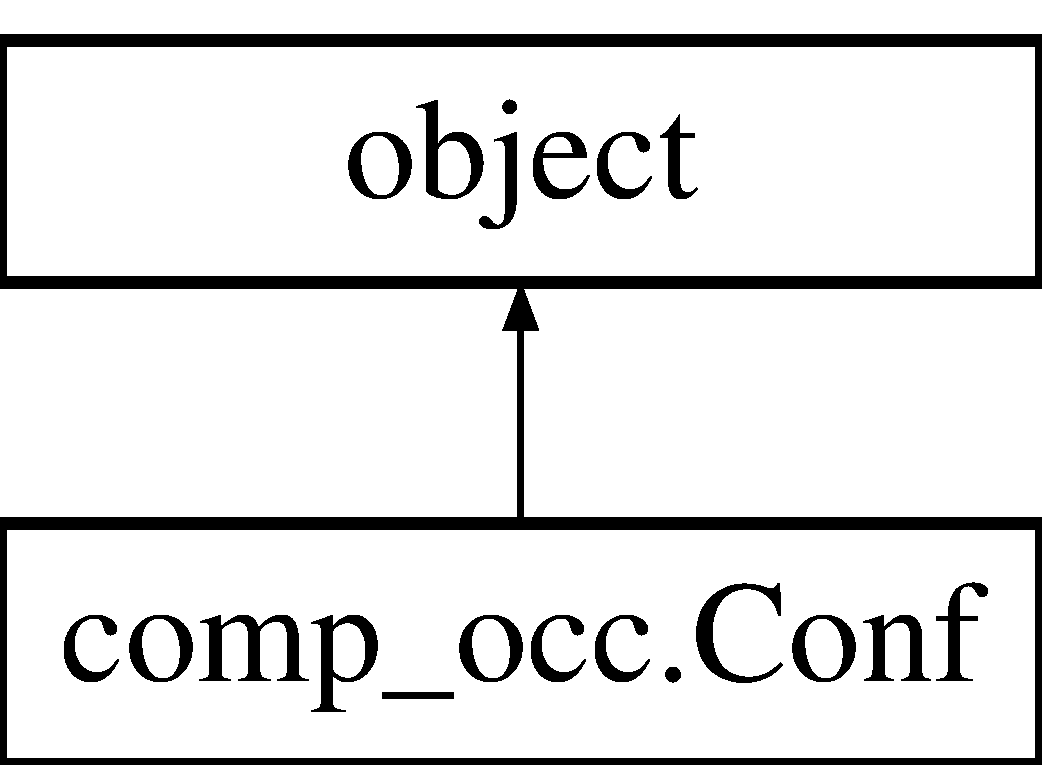
\includegraphics[height=2.000000cm]{classcomp__occ_1_1_conf}
\end{center}
\end{figure}
\subsection*{Public Member Functions}
\begin{DoxyCompactItemize}
\item 
def \hyperlink{classcomp__occ_1_1_conf_a8bcfb9626fe1990cd68bb3701a36fb5f}{\-\_\-\-\_\-init\-\_\-\-\_\-}
\end{DoxyCompactItemize}
\subsection*{Public Attributes}
\begin{DoxyCompactItemize}
\item 
\hyperlink{classcomp__occ_1_1_conf_ac424346df2bb8a9b7548c6c5768633a4}{conf\-Name}
\item 
\hyperlink{classcomp__occ_1_1_conf_a6b6a4ed6f56d67c757fe8851386fd674}{occ}
\end{DoxyCompactItemize}


\subsection{Detailed Description}
Compare the occupancy of conformers in two different runs. 

Conformer class. 

\subsection{Constructor \& Destructor Documentation}
\hypertarget{classcomp__occ_1_1_conf_a8bcfb9626fe1990cd68bb3701a36fb5f}{\index{comp\-\_\-occ\-::\-Conf@{comp\-\_\-occ\-::\-Conf}!\-\_\-\-\_\-init\-\_\-\-\_\-@{\-\_\-\-\_\-init\-\_\-\-\_\-}}
\index{\-\_\-\-\_\-init\-\_\-\-\_\-@{\-\_\-\-\_\-init\-\_\-\-\_\-}!comp_occ::Conf@{comp\-\_\-occ\-::\-Conf}}
\subsubsection[{\-\_\-\-\_\-init\-\_\-\-\_\-}]{\setlength{\rightskip}{0pt plus 5cm}def comp\-\_\-occ.\-Conf.\-\_\-\-\_\-init\-\_\-\-\_\- (
\begin{DoxyParamCaption}
\item[{}]{self, }
\item[{}]{res\-Name = {\ttfamily \char`\"{}\char`\"{}}, }
\item[{}]{occ = {\ttfamily 0.0}}
\end{DoxyParamCaption}
)}}\label{classcomp__occ_1_1_conf_a8bcfb9626fe1990cd68bb3701a36fb5f}


\subsection{Member Data Documentation}
\hypertarget{classcomp__occ_1_1_conf_ac424346df2bb8a9b7548c6c5768633a4}{\index{comp\-\_\-occ\-::\-Conf@{comp\-\_\-occ\-::\-Conf}!conf\-Name@{conf\-Name}}
\index{conf\-Name@{conf\-Name}!comp_occ::Conf@{comp\-\_\-occ\-::\-Conf}}
\subsubsection[{conf\-Name}]{\setlength{\rightskip}{0pt plus 5cm}comp\-\_\-occ.\-Conf.\-conf\-Name}}\label{classcomp__occ_1_1_conf_ac424346df2bb8a9b7548c6c5768633a4}
\hypertarget{classcomp__occ_1_1_conf_a6b6a4ed6f56d67c757fe8851386fd674}{\index{comp\-\_\-occ\-::\-Conf@{comp\-\_\-occ\-::\-Conf}!occ@{occ}}
\index{occ@{occ}!comp_occ::Conf@{comp\-\_\-occ\-::\-Conf}}
\subsubsection[{occ}]{\setlength{\rightskip}{0pt plus 5cm}comp\-\_\-occ.\-Conf.\-occ}}\label{classcomp__occ_1_1_conf_a6b6a4ed6f56d67c757fe8851386fd674}


The documentation for this class was generated from the following file\-:\begin{DoxyCompactItemize}
\item 
src/scripts/mcce/\hyperlink{comp__occ_8py}{comp\-\_\-occ.\-py}\end{DoxyCompactItemize}

\hypertarget{classxmccepy_1_1conformer_1_1_conformer}{\section{xmccepy.\-conformer.\-Conformer Class Reference}
\label{classxmccepy_1_1conformer_1_1_conformer}\index{xmccepy.\-conformer.\-Conformer@{xmccepy.\-conformer.\-Conformer}}
}


Created on Apr 1, 2014.  


Inheritance diagram for xmccepy.\-conformer.\-Conformer\-:\begin{figure}[H]
\begin{center}
\leavevmode
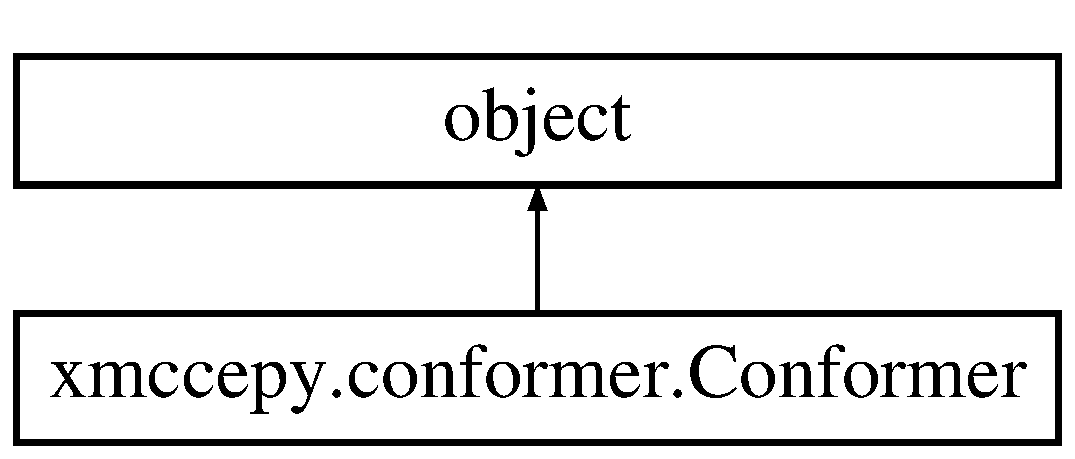
\includegraphics[height=2.000000cm]{classxmccepy_1_1conformer_1_1_conformer}
\end{center}
\end{figure}
\subsection*{Public Member Functions}
\begin{DoxyCompactItemize}
\item 
def \hyperlink{classxmccepy_1_1conformer_1_1_conformer_ace05398b4ffadf035bc7250d7da98c31}{\-\_\-\-\_\-init\-\_\-\-\_\-}
\begin{DoxyCompactList}\small\item\em Constructor. \end{DoxyCompactList}\end{DoxyCompactItemize}
\subsection*{Public Attributes}
\begin{DoxyCompactItemize}
\item 
\hyperlink{classxmccepy_1_1conformer_1_1_conformer_a717881e47510ed18cda5d11489122c5a}{conf\-Name}
\end{DoxyCompactItemize}


\subsection{Detailed Description}
Created on Apr 1, 2014. 

\begin{DoxyAuthor}{Author}
\-: xzhu \begin{DoxyVerb}Conformer class.\end{DoxyVerb}
 
\end{DoxyAuthor}


\subsection{Constructor \& Destructor Documentation}
\hypertarget{classxmccepy_1_1conformer_1_1_conformer_ace05398b4ffadf035bc7250d7da98c31}{\index{xmccepy\-::conformer\-::\-Conformer@{xmccepy\-::conformer\-::\-Conformer}!\-\_\-\-\_\-init\-\_\-\-\_\-@{\-\_\-\-\_\-init\-\_\-\-\_\-}}
\index{\-\_\-\-\_\-init\-\_\-\-\_\-@{\-\_\-\-\_\-init\-\_\-\-\_\-}!xmccepy::conformer::Conformer@{xmccepy\-::conformer\-::\-Conformer}}
\subsubsection[{\-\_\-\-\_\-init\-\_\-\-\_\-}]{\setlength{\rightskip}{0pt plus 5cm}def xmccepy.\-conformer.\-Conformer.\-\_\-\-\_\-init\-\_\-\-\_\- (
\begin{DoxyParamCaption}
\item[{}]{self}
\end{DoxyParamCaption}
)}}\label{classxmccepy_1_1conformer_1_1_conformer_ace05398b4ffadf035bc7250d7da98c31}


Constructor. 



\subsection{Member Data Documentation}
\hypertarget{classxmccepy_1_1conformer_1_1_conformer_a717881e47510ed18cda5d11489122c5a}{\index{xmccepy\-::conformer\-::\-Conformer@{xmccepy\-::conformer\-::\-Conformer}!conf\-Name@{conf\-Name}}
\index{conf\-Name@{conf\-Name}!xmccepy::conformer::Conformer@{xmccepy\-::conformer\-::\-Conformer}}
\subsubsection[{conf\-Name}]{\setlength{\rightskip}{0pt plus 5cm}xmccepy.\-conformer.\-Conformer.\-conf\-Name}}\label{classxmccepy_1_1conformer_1_1_conformer_a717881e47510ed18cda5d11489122c5a}


The documentation for this class was generated from the following file\-:\begin{DoxyCompactItemize}
\item 
src/xmccepy/\hyperlink{conformer_8py}{conformer.\-py}\end{DoxyCompactItemize}

\hypertarget{classxmccepy_1_1mp_1_1_c_o_n_f_o_r_m_e_r}{\section{xmccepy.\-mp.\-C\-O\-N\-F\-O\-R\-M\-E\-R Class Reference}
\label{classxmccepy_1_1mp_1_1_c_o_n_f_o_r_m_e_r}\index{xmccepy.\-mp.\-C\-O\-N\-F\-O\-R\-M\-E\-R@{xmccepy.\-mp.\-C\-O\-N\-F\-O\-R\-M\-E\-R}}
}
\subsection*{Public Member Functions}
\begin{DoxyCompactItemize}
\item 
def \hyperlink{classxmccepy_1_1mp_1_1_c_o_n_f_o_r_m_e_r_a371854582bd48c21b894a085ec7a9ee4}{\-\_\-\-\_\-init\-\_\-\-\_\-}
\item 
def \hyperlink{classxmccepy_1_1mp_1_1_c_o_n_f_o_r_m_e_r_a2045e40a7a38d8b544c57602d96d25e5}{initial\-\_\-by\-\_\-h3}
\item 
def \hyperlink{classxmccepy_1_1mp_1_1_c_o_n_f_o_r_m_e_r_a0c0b2d9ce8d8fb9e60edf81e618f082e}{in\-Res}
\item 
def \hyperlink{classxmccepy_1_1mp_1_1_c_o_n_f_o_r_m_e_r_a0cce02a0def0a04375125568491cc635}{load\-\_\-occ}
\end{DoxyCompactItemize}
\subsection*{Public Attributes}
\begin{DoxyCompactItemize}
\item 
\hyperlink{classxmccepy_1_1mp_1_1_c_o_n_f_o_r_m_e_r_a6a748e760bc097c1560578f42a9f857f}{atoms}
\item 
\hyperlink{classxmccepy_1_1mp_1_1_c_o_n_f_o_r_m_e_r_a9e5bf147326267319ff6e530c6fe2184}{res\-Name}
\item 
\hyperlink{classxmccepy_1_1mp_1_1_c_o_n_f_o_r_m_e_r_abd94248291d7e1014b784a61572b9b56}{res\-Seq}
\item 
\hyperlink{classxmccepy_1_1mp_1_1_c_o_n_f_o_r_m_e_r_a7200c512bdf3481f4244005873802833}{conf\-Name}
\item 
\hyperlink{classxmccepy_1_1mp_1_1_c_o_n_f_o_r_m_e_r_afc8af5d1e1ca01bc54162eef3076c0e7}{i\-Code}
\item 
\hyperlink{classxmccepy_1_1mp_1_1_c_o_n_f_o_r_m_e_r_a5e08044df96e2efc98d27d11dad2acc0}{i\-Conf}
\item 
\hyperlink{classxmccepy_1_1mp_1_1_c_o_n_f_o_r_m_e_r_a80e8729d25aa77487916dfc0b0be6c7d}{crg}
\item 
\hyperlink{classxmccepy_1_1mp_1_1_c_o_n_f_o_r_m_e_r_a62ff7372f23a1c40ea1967aaffad993c}{Em0}
\item 
\hyperlink{classxmccepy_1_1mp_1_1_c_o_n_f_o_r_m_e_r_a6b1bf83b15461d60baa91de328d195ce}{p\-Ka0}
\item 
\hyperlink{classxmccepy_1_1mp_1_1_c_o_n_f_o_r_m_e_r_ab0377ce0611af60ca84fa253d32289ca}{ne}
\item 
\hyperlink{classxmccepy_1_1mp_1_1_c_o_n_f_o_r_m_e_r_aef85f7fcfb8665f154e0fad915dbac5e}{n\-H}
\item 
\hyperlink{classxmccepy_1_1mp_1_1_c_o_n_f_o_r_m_e_r_a54266cbd09ba1b62ac724a688a077623}{F\-L}
\item 
\hyperlink{classxmccepy_1_1mp_1_1_c_o_n_f_o_r_m_e_r_aaf6ca8e069b34e52bfb9f5e95c24b859}{occ}
\item 
\hyperlink{classxmccepy_1_1mp_1_1_c_o_n_f_o_r_m_e_r_a6d2a83a118c9117dc938e954e7e5cac6}{E\-\_\-vdw0}
\item 
\hyperlink{classxmccepy_1_1mp_1_1_c_o_n_f_o_r_m_e_r_ae98aded8558a5101a760bb9b60101bac}{E\-\_\-vdw1}
\item 
\hyperlink{classxmccepy_1_1mp_1_1_c_o_n_f_o_r_m_e_r_a442b37096eecb715ef0637298e647a27}{E\-\_\-tors}
\item 
\hyperlink{classxmccepy_1_1mp_1_1_c_o_n_f_o_r_m_e_r_ab3a58e71ca1eff5c19a49c3e7ed4c682}{E\-\_\-epol}
\item 
\hyperlink{classxmccepy_1_1mp_1_1_c_o_n_f_o_r_m_e_r_a05f3e253b3e75d0868f55babb6d39d61}{E\-\_\-dsolv}
\item 
\hyperlink{classxmccepy_1_1mp_1_1_c_o_n_f_o_r_m_e_r_abd6de497b74afb9d65545f1581a2b88d}{extra}
\item 
\hyperlink{classxmccepy_1_1mp_1_1_c_o_n_f_o_r_m_e_r_a78d0c3efc8bbf322e759a475e7eb74e0}{history}
\item 
\hyperlink{classxmccepy_1_1mp_1_1_c_o_n_f_o_r_m_e_r_ac1880aa3dad24483cb41a4bf5da0c640}{focc}
\item 
\hyperlink{classxmccepy_1_1mp_1_1_c_o_n_f_o_r_m_e_r_a32f981febbee2d7b5e6e9099f1ced82c}{E\-\_\-extra}
\end{DoxyCompactItemize}


\subsection{Constructor \& Destructor Documentation}
\hypertarget{classxmccepy_1_1mp_1_1_c_o_n_f_o_r_m_e_r_a371854582bd48c21b894a085ec7a9ee4}{\index{xmccepy\-::mp\-::\-C\-O\-N\-F\-O\-R\-M\-E\-R@{xmccepy\-::mp\-::\-C\-O\-N\-F\-O\-R\-M\-E\-R}!\-\_\-\-\_\-init\-\_\-\-\_\-@{\-\_\-\-\_\-init\-\_\-\-\_\-}}
\index{\-\_\-\-\_\-init\-\_\-\-\_\-@{\-\_\-\-\_\-init\-\_\-\-\_\-}!xmccepy::mp::CONFORMER@{xmccepy\-::mp\-::\-C\-O\-N\-F\-O\-R\-M\-E\-R}}
\subsubsection[{\-\_\-\-\_\-init\-\_\-\-\_\-}]{\setlength{\rightskip}{0pt plus 5cm}def xmccepy.\-mp.\-C\-O\-N\-F\-O\-R\-M\-E\-R.\-\_\-\-\_\-init\-\_\-\-\_\- (
\begin{DoxyParamCaption}
\item[{}]{self}
\end{DoxyParamCaption}
)}}\label{classxmccepy_1_1mp_1_1_c_o_n_f_o_r_m_e_r_a371854582bd48c21b894a085ec7a9ee4}


\subsection{Member Function Documentation}
\hypertarget{classxmccepy_1_1mp_1_1_c_o_n_f_o_r_m_e_r_a2045e40a7a38d8b544c57602d96d25e5}{\index{xmccepy\-::mp\-::\-C\-O\-N\-F\-O\-R\-M\-E\-R@{xmccepy\-::mp\-::\-C\-O\-N\-F\-O\-R\-M\-E\-R}!initial\-\_\-by\-\_\-h3@{initial\-\_\-by\-\_\-h3}}
\index{initial\-\_\-by\-\_\-h3@{initial\-\_\-by\-\_\-h3}!xmccepy::mp::CONFORMER@{xmccepy\-::mp\-::\-C\-O\-N\-F\-O\-R\-M\-E\-R}}
\subsubsection[{initial\-\_\-by\-\_\-h3}]{\setlength{\rightskip}{0pt plus 5cm}def xmccepy.\-mp.\-C\-O\-N\-F\-O\-R\-M\-E\-R.\-initial\-\_\-by\-\_\-h3 (
\begin{DoxyParamCaption}
\item[{}]{line}
\end{DoxyParamCaption}
)}}\label{classxmccepy_1_1mp_1_1_c_o_n_f_o_r_m_e_r_a2045e40a7a38d8b544c57602d96d25e5}
\hypertarget{classxmccepy_1_1mp_1_1_c_o_n_f_o_r_m_e_r_a0c0b2d9ce8d8fb9e60edf81e618f082e}{\index{xmccepy\-::mp\-::\-C\-O\-N\-F\-O\-R\-M\-E\-R@{xmccepy\-::mp\-::\-C\-O\-N\-F\-O\-R\-M\-E\-R}!in\-Res@{in\-Res}}
\index{in\-Res@{in\-Res}!xmccepy::mp::CONFORMER@{xmccepy\-::mp\-::\-C\-O\-N\-F\-O\-R\-M\-E\-R}}
\subsubsection[{in\-Res}]{\setlength{\rightskip}{0pt plus 5cm}def xmccepy.\-mp.\-C\-O\-N\-F\-O\-R\-M\-E\-R.\-in\-Res (
\begin{DoxyParamCaption}
\item[{}]{res\-Name}
\end{DoxyParamCaption}
)}}\label{classxmccepy_1_1mp_1_1_c_o_n_f_o_r_m_e_r_a0c0b2d9ce8d8fb9e60edf81e618f082e}
\hypertarget{classxmccepy_1_1mp_1_1_c_o_n_f_o_r_m_e_r_a0cce02a0def0a04375125568491cc635}{\index{xmccepy\-::mp\-::\-C\-O\-N\-F\-O\-R\-M\-E\-R@{xmccepy\-::mp\-::\-C\-O\-N\-F\-O\-R\-M\-E\-R}!load\-\_\-occ@{load\-\_\-occ}}
\index{load\-\_\-occ@{load\-\_\-occ}!xmccepy::mp::CONFORMER@{xmccepy\-::mp\-::\-C\-O\-N\-F\-O\-R\-M\-E\-R}}
\subsubsection[{load\-\_\-occ}]{\setlength{\rightskip}{0pt plus 5cm}def xmccepy.\-mp.\-C\-O\-N\-F\-O\-R\-M\-E\-R.\-load\-\_\-occ (
\begin{DoxyParamCaption}
\item[{}]{line}
\end{DoxyParamCaption}
)}}\label{classxmccepy_1_1mp_1_1_c_o_n_f_o_r_m_e_r_a0cce02a0def0a04375125568491cc635}


\subsection{Member Data Documentation}
\hypertarget{classxmccepy_1_1mp_1_1_c_o_n_f_o_r_m_e_r_a6a748e760bc097c1560578f42a9f857f}{\index{xmccepy\-::mp\-::\-C\-O\-N\-F\-O\-R\-M\-E\-R@{xmccepy\-::mp\-::\-C\-O\-N\-F\-O\-R\-M\-E\-R}!atoms@{atoms}}
\index{atoms@{atoms}!xmccepy::mp::CONFORMER@{xmccepy\-::mp\-::\-C\-O\-N\-F\-O\-R\-M\-E\-R}}
\subsubsection[{atoms}]{\setlength{\rightskip}{0pt plus 5cm}xmccepy.\-mp.\-C\-O\-N\-F\-O\-R\-M\-E\-R.\-atoms}}\label{classxmccepy_1_1mp_1_1_c_o_n_f_o_r_m_e_r_a6a748e760bc097c1560578f42a9f857f}
\hypertarget{classxmccepy_1_1mp_1_1_c_o_n_f_o_r_m_e_r_a7200c512bdf3481f4244005873802833}{\index{xmccepy\-::mp\-::\-C\-O\-N\-F\-O\-R\-M\-E\-R@{xmccepy\-::mp\-::\-C\-O\-N\-F\-O\-R\-M\-E\-R}!conf\-Name@{conf\-Name}}
\index{conf\-Name@{conf\-Name}!xmccepy::mp::CONFORMER@{xmccepy\-::mp\-::\-C\-O\-N\-F\-O\-R\-M\-E\-R}}
\subsubsection[{conf\-Name}]{\setlength{\rightskip}{0pt plus 5cm}xmccepy.\-mp.\-C\-O\-N\-F\-O\-R\-M\-E\-R.\-conf\-Name}}\label{classxmccepy_1_1mp_1_1_c_o_n_f_o_r_m_e_r_a7200c512bdf3481f4244005873802833}
\hypertarget{classxmccepy_1_1mp_1_1_c_o_n_f_o_r_m_e_r_a80e8729d25aa77487916dfc0b0be6c7d}{\index{xmccepy\-::mp\-::\-C\-O\-N\-F\-O\-R\-M\-E\-R@{xmccepy\-::mp\-::\-C\-O\-N\-F\-O\-R\-M\-E\-R}!crg@{crg}}
\index{crg@{crg}!xmccepy::mp::CONFORMER@{xmccepy\-::mp\-::\-C\-O\-N\-F\-O\-R\-M\-E\-R}}
\subsubsection[{crg}]{\setlength{\rightskip}{0pt plus 5cm}xmccepy.\-mp.\-C\-O\-N\-F\-O\-R\-M\-E\-R.\-crg}}\label{classxmccepy_1_1mp_1_1_c_o_n_f_o_r_m_e_r_a80e8729d25aa77487916dfc0b0be6c7d}
\hypertarget{classxmccepy_1_1mp_1_1_c_o_n_f_o_r_m_e_r_a05f3e253b3e75d0868f55babb6d39d61}{\index{xmccepy\-::mp\-::\-C\-O\-N\-F\-O\-R\-M\-E\-R@{xmccepy\-::mp\-::\-C\-O\-N\-F\-O\-R\-M\-E\-R}!E\-\_\-dsolv@{E\-\_\-dsolv}}
\index{E\-\_\-dsolv@{E\-\_\-dsolv}!xmccepy::mp::CONFORMER@{xmccepy\-::mp\-::\-C\-O\-N\-F\-O\-R\-M\-E\-R}}
\subsubsection[{E\-\_\-dsolv}]{\setlength{\rightskip}{0pt plus 5cm}xmccepy.\-mp.\-C\-O\-N\-F\-O\-R\-M\-E\-R.\-E\-\_\-dsolv}}\label{classxmccepy_1_1mp_1_1_c_o_n_f_o_r_m_e_r_a05f3e253b3e75d0868f55babb6d39d61}
\hypertarget{classxmccepy_1_1mp_1_1_c_o_n_f_o_r_m_e_r_ab3a58e71ca1eff5c19a49c3e7ed4c682}{\index{xmccepy\-::mp\-::\-C\-O\-N\-F\-O\-R\-M\-E\-R@{xmccepy\-::mp\-::\-C\-O\-N\-F\-O\-R\-M\-E\-R}!E\-\_\-epol@{E\-\_\-epol}}
\index{E\-\_\-epol@{E\-\_\-epol}!xmccepy::mp::CONFORMER@{xmccepy\-::mp\-::\-C\-O\-N\-F\-O\-R\-M\-E\-R}}
\subsubsection[{E\-\_\-epol}]{\setlength{\rightskip}{0pt plus 5cm}xmccepy.\-mp.\-C\-O\-N\-F\-O\-R\-M\-E\-R.\-E\-\_\-epol}}\label{classxmccepy_1_1mp_1_1_c_o_n_f_o_r_m_e_r_ab3a58e71ca1eff5c19a49c3e7ed4c682}
\hypertarget{classxmccepy_1_1mp_1_1_c_o_n_f_o_r_m_e_r_a32f981febbee2d7b5e6e9099f1ced82c}{\index{xmccepy\-::mp\-::\-C\-O\-N\-F\-O\-R\-M\-E\-R@{xmccepy\-::mp\-::\-C\-O\-N\-F\-O\-R\-M\-E\-R}!E\-\_\-extra@{E\-\_\-extra}}
\index{E\-\_\-extra@{E\-\_\-extra}!xmccepy::mp::CONFORMER@{xmccepy\-::mp\-::\-C\-O\-N\-F\-O\-R\-M\-E\-R}}
\subsubsection[{E\-\_\-extra}]{\setlength{\rightskip}{0pt plus 5cm}xmccepy.\-mp.\-C\-O\-N\-F\-O\-R\-M\-E\-R.\-E\-\_\-extra}}\label{classxmccepy_1_1mp_1_1_c_o_n_f_o_r_m_e_r_a32f981febbee2d7b5e6e9099f1ced82c}
\hypertarget{classxmccepy_1_1mp_1_1_c_o_n_f_o_r_m_e_r_a442b37096eecb715ef0637298e647a27}{\index{xmccepy\-::mp\-::\-C\-O\-N\-F\-O\-R\-M\-E\-R@{xmccepy\-::mp\-::\-C\-O\-N\-F\-O\-R\-M\-E\-R}!E\-\_\-tors@{E\-\_\-tors}}
\index{E\-\_\-tors@{E\-\_\-tors}!xmccepy::mp::CONFORMER@{xmccepy\-::mp\-::\-C\-O\-N\-F\-O\-R\-M\-E\-R}}
\subsubsection[{E\-\_\-tors}]{\setlength{\rightskip}{0pt plus 5cm}xmccepy.\-mp.\-C\-O\-N\-F\-O\-R\-M\-E\-R.\-E\-\_\-tors}}\label{classxmccepy_1_1mp_1_1_c_o_n_f_o_r_m_e_r_a442b37096eecb715ef0637298e647a27}
\hypertarget{classxmccepy_1_1mp_1_1_c_o_n_f_o_r_m_e_r_a6d2a83a118c9117dc938e954e7e5cac6}{\index{xmccepy\-::mp\-::\-C\-O\-N\-F\-O\-R\-M\-E\-R@{xmccepy\-::mp\-::\-C\-O\-N\-F\-O\-R\-M\-E\-R}!E\-\_\-vdw0@{E\-\_\-vdw0}}
\index{E\-\_\-vdw0@{E\-\_\-vdw0}!xmccepy::mp::CONFORMER@{xmccepy\-::mp\-::\-C\-O\-N\-F\-O\-R\-M\-E\-R}}
\subsubsection[{E\-\_\-vdw0}]{\setlength{\rightskip}{0pt plus 5cm}xmccepy.\-mp.\-C\-O\-N\-F\-O\-R\-M\-E\-R.\-E\-\_\-vdw0}}\label{classxmccepy_1_1mp_1_1_c_o_n_f_o_r_m_e_r_a6d2a83a118c9117dc938e954e7e5cac6}
\hypertarget{classxmccepy_1_1mp_1_1_c_o_n_f_o_r_m_e_r_ae98aded8558a5101a760bb9b60101bac}{\index{xmccepy\-::mp\-::\-C\-O\-N\-F\-O\-R\-M\-E\-R@{xmccepy\-::mp\-::\-C\-O\-N\-F\-O\-R\-M\-E\-R}!E\-\_\-vdw1@{E\-\_\-vdw1}}
\index{E\-\_\-vdw1@{E\-\_\-vdw1}!xmccepy::mp::CONFORMER@{xmccepy\-::mp\-::\-C\-O\-N\-F\-O\-R\-M\-E\-R}}
\subsubsection[{E\-\_\-vdw1}]{\setlength{\rightskip}{0pt plus 5cm}xmccepy.\-mp.\-C\-O\-N\-F\-O\-R\-M\-E\-R.\-E\-\_\-vdw1}}\label{classxmccepy_1_1mp_1_1_c_o_n_f_o_r_m_e_r_ae98aded8558a5101a760bb9b60101bac}
\hypertarget{classxmccepy_1_1mp_1_1_c_o_n_f_o_r_m_e_r_a62ff7372f23a1c40ea1967aaffad993c}{\index{xmccepy\-::mp\-::\-C\-O\-N\-F\-O\-R\-M\-E\-R@{xmccepy\-::mp\-::\-C\-O\-N\-F\-O\-R\-M\-E\-R}!Em0@{Em0}}
\index{Em0@{Em0}!xmccepy::mp::CONFORMER@{xmccepy\-::mp\-::\-C\-O\-N\-F\-O\-R\-M\-E\-R}}
\subsubsection[{Em0}]{\setlength{\rightskip}{0pt plus 5cm}xmccepy.\-mp.\-C\-O\-N\-F\-O\-R\-M\-E\-R.\-Em0}}\label{classxmccepy_1_1mp_1_1_c_o_n_f_o_r_m_e_r_a62ff7372f23a1c40ea1967aaffad993c}
\hypertarget{classxmccepy_1_1mp_1_1_c_o_n_f_o_r_m_e_r_abd6de497b74afb9d65545f1581a2b88d}{\index{xmccepy\-::mp\-::\-C\-O\-N\-F\-O\-R\-M\-E\-R@{xmccepy\-::mp\-::\-C\-O\-N\-F\-O\-R\-M\-E\-R}!extra@{extra}}
\index{extra@{extra}!xmccepy::mp::CONFORMER@{xmccepy\-::mp\-::\-C\-O\-N\-F\-O\-R\-M\-E\-R}}
\subsubsection[{extra}]{\setlength{\rightskip}{0pt plus 5cm}xmccepy.\-mp.\-C\-O\-N\-F\-O\-R\-M\-E\-R.\-extra}}\label{classxmccepy_1_1mp_1_1_c_o_n_f_o_r_m_e_r_abd6de497b74afb9d65545f1581a2b88d}
\hypertarget{classxmccepy_1_1mp_1_1_c_o_n_f_o_r_m_e_r_a54266cbd09ba1b62ac724a688a077623}{\index{xmccepy\-::mp\-::\-C\-O\-N\-F\-O\-R\-M\-E\-R@{xmccepy\-::mp\-::\-C\-O\-N\-F\-O\-R\-M\-E\-R}!F\-L@{F\-L}}
\index{F\-L@{F\-L}!xmccepy::mp::CONFORMER@{xmccepy\-::mp\-::\-C\-O\-N\-F\-O\-R\-M\-E\-R}}
\subsubsection[{F\-L}]{\setlength{\rightskip}{0pt plus 5cm}xmccepy.\-mp.\-C\-O\-N\-F\-O\-R\-M\-E\-R.\-F\-L}}\label{classxmccepy_1_1mp_1_1_c_o_n_f_o_r_m_e_r_a54266cbd09ba1b62ac724a688a077623}
\hypertarget{classxmccepy_1_1mp_1_1_c_o_n_f_o_r_m_e_r_ac1880aa3dad24483cb41a4bf5da0c640}{\index{xmccepy\-::mp\-::\-C\-O\-N\-F\-O\-R\-M\-E\-R@{xmccepy\-::mp\-::\-C\-O\-N\-F\-O\-R\-M\-E\-R}!focc@{focc}}
\index{focc@{focc}!xmccepy::mp::CONFORMER@{xmccepy\-::mp\-::\-C\-O\-N\-F\-O\-R\-M\-E\-R}}
\subsubsection[{focc}]{\setlength{\rightskip}{0pt plus 5cm}xmccepy.\-mp.\-C\-O\-N\-F\-O\-R\-M\-E\-R.\-focc}}\label{classxmccepy_1_1mp_1_1_c_o_n_f_o_r_m_e_r_ac1880aa3dad24483cb41a4bf5da0c640}
\hypertarget{classxmccepy_1_1mp_1_1_c_o_n_f_o_r_m_e_r_a78d0c3efc8bbf322e759a475e7eb74e0}{\index{xmccepy\-::mp\-::\-C\-O\-N\-F\-O\-R\-M\-E\-R@{xmccepy\-::mp\-::\-C\-O\-N\-F\-O\-R\-M\-E\-R}!history@{history}}
\index{history@{history}!xmccepy::mp::CONFORMER@{xmccepy\-::mp\-::\-C\-O\-N\-F\-O\-R\-M\-E\-R}}
\subsubsection[{history}]{\setlength{\rightskip}{0pt plus 5cm}xmccepy.\-mp.\-C\-O\-N\-F\-O\-R\-M\-E\-R.\-history}}\label{classxmccepy_1_1mp_1_1_c_o_n_f_o_r_m_e_r_a78d0c3efc8bbf322e759a475e7eb74e0}
\hypertarget{classxmccepy_1_1mp_1_1_c_o_n_f_o_r_m_e_r_afc8af5d1e1ca01bc54162eef3076c0e7}{\index{xmccepy\-::mp\-::\-C\-O\-N\-F\-O\-R\-M\-E\-R@{xmccepy\-::mp\-::\-C\-O\-N\-F\-O\-R\-M\-E\-R}!i\-Code@{i\-Code}}
\index{i\-Code@{i\-Code}!xmccepy::mp::CONFORMER@{xmccepy\-::mp\-::\-C\-O\-N\-F\-O\-R\-M\-E\-R}}
\subsubsection[{i\-Code}]{\setlength{\rightskip}{0pt plus 5cm}xmccepy.\-mp.\-C\-O\-N\-F\-O\-R\-M\-E\-R.\-i\-Code}}\label{classxmccepy_1_1mp_1_1_c_o_n_f_o_r_m_e_r_afc8af5d1e1ca01bc54162eef3076c0e7}
\hypertarget{classxmccepy_1_1mp_1_1_c_o_n_f_o_r_m_e_r_a5e08044df96e2efc98d27d11dad2acc0}{\index{xmccepy\-::mp\-::\-C\-O\-N\-F\-O\-R\-M\-E\-R@{xmccepy\-::mp\-::\-C\-O\-N\-F\-O\-R\-M\-E\-R}!i\-Conf@{i\-Conf}}
\index{i\-Conf@{i\-Conf}!xmccepy::mp::CONFORMER@{xmccepy\-::mp\-::\-C\-O\-N\-F\-O\-R\-M\-E\-R}}
\subsubsection[{i\-Conf}]{\setlength{\rightskip}{0pt plus 5cm}xmccepy.\-mp.\-C\-O\-N\-F\-O\-R\-M\-E\-R.\-i\-Conf}}\label{classxmccepy_1_1mp_1_1_c_o_n_f_o_r_m_e_r_a5e08044df96e2efc98d27d11dad2acc0}
\hypertarget{classxmccepy_1_1mp_1_1_c_o_n_f_o_r_m_e_r_ab0377ce0611af60ca84fa253d32289ca}{\index{xmccepy\-::mp\-::\-C\-O\-N\-F\-O\-R\-M\-E\-R@{xmccepy\-::mp\-::\-C\-O\-N\-F\-O\-R\-M\-E\-R}!ne@{ne}}
\index{ne@{ne}!xmccepy::mp::CONFORMER@{xmccepy\-::mp\-::\-C\-O\-N\-F\-O\-R\-M\-E\-R}}
\subsubsection[{ne}]{\setlength{\rightskip}{0pt plus 5cm}xmccepy.\-mp.\-C\-O\-N\-F\-O\-R\-M\-E\-R.\-ne}}\label{classxmccepy_1_1mp_1_1_c_o_n_f_o_r_m_e_r_ab0377ce0611af60ca84fa253d32289ca}
\hypertarget{classxmccepy_1_1mp_1_1_c_o_n_f_o_r_m_e_r_aef85f7fcfb8665f154e0fad915dbac5e}{\index{xmccepy\-::mp\-::\-C\-O\-N\-F\-O\-R\-M\-E\-R@{xmccepy\-::mp\-::\-C\-O\-N\-F\-O\-R\-M\-E\-R}!n\-H@{n\-H}}
\index{n\-H@{n\-H}!xmccepy::mp::CONFORMER@{xmccepy\-::mp\-::\-C\-O\-N\-F\-O\-R\-M\-E\-R}}
\subsubsection[{n\-H}]{\setlength{\rightskip}{0pt plus 5cm}xmccepy.\-mp.\-C\-O\-N\-F\-O\-R\-M\-E\-R.\-n\-H}}\label{classxmccepy_1_1mp_1_1_c_o_n_f_o_r_m_e_r_aef85f7fcfb8665f154e0fad915dbac5e}
\hypertarget{classxmccepy_1_1mp_1_1_c_o_n_f_o_r_m_e_r_aaf6ca8e069b34e52bfb9f5e95c24b859}{\index{xmccepy\-::mp\-::\-C\-O\-N\-F\-O\-R\-M\-E\-R@{xmccepy\-::mp\-::\-C\-O\-N\-F\-O\-R\-M\-E\-R}!occ@{occ}}
\index{occ@{occ}!xmccepy::mp::CONFORMER@{xmccepy\-::mp\-::\-C\-O\-N\-F\-O\-R\-M\-E\-R}}
\subsubsection[{occ}]{\setlength{\rightskip}{0pt plus 5cm}xmccepy.\-mp.\-C\-O\-N\-F\-O\-R\-M\-E\-R.\-occ}}\label{classxmccepy_1_1mp_1_1_c_o_n_f_o_r_m_e_r_aaf6ca8e069b34e52bfb9f5e95c24b859}
\hypertarget{classxmccepy_1_1mp_1_1_c_o_n_f_o_r_m_e_r_a6b1bf83b15461d60baa91de328d195ce}{\index{xmccepy\-::mp\-::\-C\-O\-N\-F\-O\-R\-M\-E\-R@{xmccepy\-::mp\-::\-C\-O\-N\-F\-O\-R\-M\-E\-R}!p\-Ka0@{p\-Ka0}}
\index{p\-Ka0@{p\-Ka0}!xmccepy::mp::CONFORMER@{xmccepy\-::mp\-::\-C\-O\-N\-F\-O\-R\-M\-E\-R}}
\subsubsection[{p\-Ka0}]{\setlength{\rightskip}{0pt plus 5cm}xmccepy.\-mp.\-C\-O\-N\-F\-O\-R\-M\-E\-R.\-p\-Ka0}}\label{classxmccepy_1_1mp_1_1_c_o_n_f_o_r_m_e_r_a6b1bf83b15461d60baa91de328d195ce}
\hypertarget{classxmccepy_1_1mp_1_1_c_o_n_f_o_r_m_e_r_a9e5bf147326267319ff6e530c6fe2184}{\index{xmccepy\-::mp\-::\-C\-O\-N\-F\-O\-R\-M\-E\-R@{xmccepy\-::mp\-::\-C\-O\-N\-F\-O\-R\-M\-E\-R}!res\-Name@{res\-Name}}
\index{res\-Name@{res\-Name}!xmccepy::mp::CONFORMER@{xmccepy\-::mp\-::\-C\-O\-N\-F\-O\-R\-M\-E\-R}}
\subsubsection[{res\-Name}]{\setlength{\rightskip}{0pt plus 5cm}xmccepy.\-mp.\-C\-O\-N\-F\-O\-R\-M\-E\-R.\-res\-Name}}\label{classxmccepy_1_1mp_1_1_c_o_n_f_o_r_m_e_r_a9e5bf147326267319ff6e530c6fe2184}
\hypertarget{classxmccepy_1_1mp_1_1_c_o_n_f_o_r_m_e_r_abd94248291d7e1014b784a61572b9b56}{\index{xmccepy\-::mp\-::\-C\-O\-N\-F\-O\-R\-M\-E\-R@{xmccepy\-::mp\-::\-C\-O\-N\-F\-O\-R\-M\-E\-R}!res\-Seq@{res\-Seq}}
\index{res\-Seq@{res\-Seq}!xmccepy::mp::CONFORMER@{xmccepy\-::mp\-::\-C\-O\-N\-F\-O\-R\-M\-E\-R}}
\subsubsection[{res\-Seq}]{\setlength{\rightskip}{0pt plus 5cm}xmccepy.\-mp.\-C\-O\-N\-F\-O\-R\-M\-E\-R.\-res\-Seq}}\label{classxmccepy_1_1mp_1_1_c_o_n_f_o_r_m_e_r_abd94248291d7e1014b784a61572b9b56}


The documentation for this class was generated from the following file\-:\begin{DoxyCompactItemize}
\item 
src/xmccepy/\hyperlink{mp_8py}{mp.\-py}\end{DoxyCompactItemize}

\hypertarget{classxmccepy_1_1corr_1_1_corr}{\section{xmccepy.\-corr.\-Corr Class Reference}
\label{classxmccepy_1_1corr_1_1_corr}\index{xmccepy.\-corr.\-Corr@{xmccepy.\-corr.\-Corr}}
}


A class for the coordinate of a position.  


Inheritance diagram for xmccepy.\-corr.\-Corr\-:\begin{figure}[H]
\begin{center}
\leavevmode
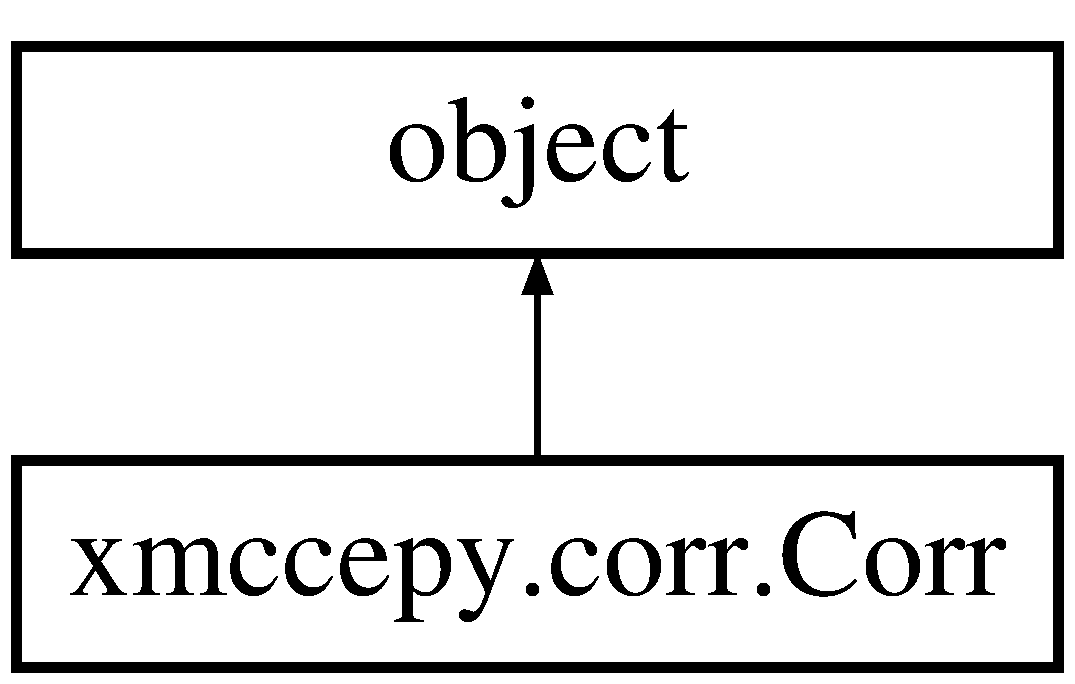
\includegraphics[height=2.000000cm]{classxmccepy_1_1corr_1_1_corr}
\end{center}
\end{figure}
\subsection*{Public Member Functions}
\begin{DoxyCompactItemize}
\item 
def \hyperlink{classxmccepy_1_1corr_1_1_corr_ab9af2823d754b0458bd814cc0ffa6d55}{\-\_\-\-\_\-init\-\_\-\-\_\-}
\begin{DoxyCompactList}\small\item\em Constructor. \end{DoxyCompactList}\item 
def \hyperlink{classxmccepy_1_1corr_1_1_corr_afdc411e79f72e2728c9eb5db1fba693f}{set}
\begin{DoxyCompactList}\small\item\em Set the x, y, z values of a coordinate. \end{DoxyCompactList}\end{DoxyCompactItemize}
\subsection*{Public Attributes}
\begin{DoxyCompactItemize}
\item 
\hyperlink{classxmccepy_1_1corr_1_1_corr_af92bf6894f8092d64bebdd641fba09f7}{x}
\item 
\hyperlink{classxmccepy_1_1corr_1_1_corr_a6a9298c2b8c4747dbd514dcde6b4e98d}{y}
\item 
\hyperlink{classxmccepy_1_1corr_1_1_corr_af4b31d22cd5524607542063be5b86a82}{z}
\end{DoxyCompactItemize}


\subsection{Detailed Description}
A class for the coordinate of a position. 

Created on Apr 1, 2014

\begin{DoxyAuthor}{Author}
\-: xzhu \begin{DoxyVerb}Corrdinate class.\end{DoxyVerb}
 
\end{DoxyAuthor}


\subsection{Constructor \& Destructor Documentation}
\hypertarget{classxmccepy_1_1corr_1_1_corr_ab9af2823d754b0458bd814cc0ffa6d55}{\index{xmccepy\-::corr\-::\-Corr@{xmccepy\-::corr\-::\-Corr}!\-\_\-\-\_\-init\-\_\-\-\_\-@{\-\_\-\-\_\-init\-\_\-\-\_\-}}
\index{\-\_\-\-\_\-init\-\_\-\-\_\-@{\-\_\-\-\_\-init\-\_\-\-\_\-}!xmccepy::corr::Corr@{xmccepy\-::corr\-::\-Corr}}
\subsubsection[{\-\_\-\-\_\-init\-\_\-\-\_\-}]{\setlength{\rightskip}{0pt plus 5cm}def xmccepy.\-corr.\-Corr.\-\_\-\-\_\-init\-\_\-\-\_\- (
\begin{DoxyParamCaption}
\item[{}]{self, }
\item[{}]{x = {\ttfamily 0.0}, }
\item[{}]{y = {\ttfamily 0.0}, }
\item[{}]{z = {\ttfamily 0.0}}
\end{DoxyParamCaption}
)}}\label{classxmccepy_1_1corr_1_1_corr_ab9af2823d754b0458bd814cc0ffa6d55}


Constructor. 



\subsection{Member Function Documentation}
\hypertarget{classxmccepy_1_1corr_1_1_corr_afdc411e79f72e2728c9eb5db1fba693f}{\index{xmccepy\-::corr\-::\-Corr@{xmccepy\-::corr\-::\-Corr}!set@{set}}
\index{set@{set}!xmccepy::corr::Corr@{xmccepy\-::corr\-::\-Corr}}
\subsubsection[{set}]{\setlength{\rightskip}{0pt plus 5cm}def xmccepy.\-corr.\-Corr.\-set (
\begin{DoxyParamCaption}
\item[{}]{self, }
\item[{}]{x = {\ttfamily 0.0}, }
\item[{}]{y = {\ttfamily 0.0}, }
\item[{}]{z = {\ttfamily 0.0}}
\end{DoxyParamCaption}
)}}\label{classxmccepy_1_1corr_1_1_corr_afdc411e79f72e2728c9eb5db1fba693f}


Set the x, y, z values of a coordinate. 



\subsection{Member Data Documentation}
\hypertarget{classxmccepy_1_1corr_1_1_corr_af92bf6894f8092d64bebdd641fba09f7}{\index{xmccepy\-::corr\-::\-Corr@{xmccepy\-::corr\-::\-Corr}!x@{x}}
\index{x@{x}!xmccepy::corr::Corr@{xmccepy\-::corr\-::\-Corr}}
\subsubsection[{x}]{\setlength{\rightskip}{0pt plus 5cm}xmccepy.\-corr.\-Corr.\-x}}\label{classxmccepy_1_1corr_1_1_corr_af92bf6894f8092d64bebdd641fba09f7}
\hypertarget{classxmccepy_1_1corr_1_1_corr_a6a9298c2b8c4747dbd514dcde6b4e98d}{\index{xmccepy\-::corr\-::\-Corr@{xmccepy\-::corr\-::\-Corr}!y@{y}}
\index{y@{y}!xmccepy::corr::Corr@{xmccepy\-::corr\-::\-Corr}}
\subsubsection[{y}]{\setlength{\rightskip}{0pt plus 5cm}xmccepy.\-corr.\-Corr.\-y}}\label{classxmccepy_1_1corr_1_1_corr_a6a9298c2b8c4747dbd514dcde6b4e98d}
\hypertarget{classxmccepy_1_1corr_1_1_corr_af4b31d22cd5524607542063be5b86a82}{\index{xmccepy\-::corr\-::\-Corr@{xmccepy\-::corr\-::\-Corr}!z@{z}}
\index{z@{z}!xmccepy::corr::Corr@{xmccepy\-::corr\-::\-Corr}}
\subsubsection[{z}]{\setlength{\rightskip}{0pt plus 5cm}xmccepy.\-corr.\-Corr.\-z}}\label{classxmccepy_1_1corr_1_1_corr_af4b31d22cd5524607542063be5b86a82}


The documentation for this class was generated from the following file\-:\begin{DoxyCompactItemize}
\item 
src/xmccepy/\hyperlink{corr_8py}{corr.\-py}\end{DoxyCompactItemize}

\hypertarget{classparse__mc__out_1_1_energy_traject}{\section{parse\-\_\-mc\-\_\-out.\-Energy\-Traject Class Reference}
\label{classparse__mc__out_1_1_energy_traject}\index{parse\-\_\-mc\-\_\-out.\-Energy\-Traject@{parse\-\_\-mc\-\_\-out.\-Energy\-Traject}}
}
Inheritance diagram for parse\-\_\-mc\-\_\-out.\-Energy\-Traject\-:\begin{figure}[H]
\begin{center}
\leavevmode
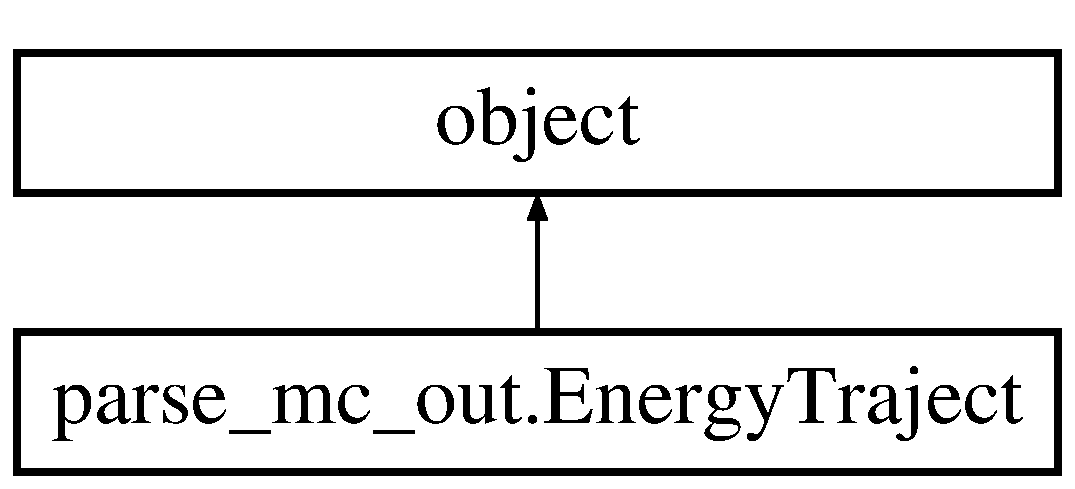
\includegraphics[height=2.000000cm]{classparse__mc__out_1_1_energy_traject}
\end{center}
\end{figure}
\subsection*{Public Member Functions}
\begin{DoxyCompactItemize}
\item 
def \hyperlink{classparse__mc__out_1_1_energy_traject_a12f6574577648b4370fdc0f24f253d67}{\-\_\-\-\_\-init\-\_\-\-\_\-}
\item 
def \hyperlink{classparse__mc__out_1_1_energy_traject_af68bcdb88e803e16948cb805b744ba2e}{add\-Step}
\item 
def \hyperlink{classparse__mc__out_1_1_energy_traject_a051802c7c03d2d06f03ff784627f14fa}{plot}
\end{DoxyCompactItemize}
\subsection*{Public Attributes}
\begin{DoxyCompactItemize}
\item 
\hyperlink{classparse__mc__out_1_1_energy_traject_a827f43a08531e3bd0b1e51e216a06a9c}{steps}
\item 
\hyperlink{classparse__mc__out_1_1_energy_traject_afec19ac593c5be2a29167a6ec21b951f}{energies}
\item 
\hyperlink{classparse__mc__out_1_1_energy_traject_a5dd33d48943a8013e66d012e0fd408fc}{mc\-Id}
\end{DoxyCompactItemize}


\subsection{Constructor \& Destructor Documentation}
\hypertarget{classparse__mc__out_1_1_energy_traject_a12f6574577648b4370fdc0f24f253d67}{\index{parse\-\_\-mc\-\_\-out\-::\-Energy\-Traject@{parse\-\_\-mc\-\_\-out\-::\-Energy\-Traject}!\-\_\-\-\_\-init\-\_\-\-\_\-@{\-\_\-\-\_\-init\-\_\-\-\_\-}}
\index{\-\_\-\-\_\-init\-\_\-\-\_\-@{\-\_\-\-\_\-init\-\_\-\-\_\-}!parse_mc_out::EnergyTraject@{parse\-\_\-mc\-\_\-out\-::\-Energy\-Traject}}
\subsubsection[{\-\_\-\-\_\-init\-\_\-\-\_\-}]{\setlength{\rightskip}{0pt plus 5cm}def parse\-\_\-mc\-\_\-out.\-Energy\-Traject.\-\_\-\-\_\-init\-\_\-\-\_\- (
\begin{DoxyParamCaption}
\item[{}]{self}
\end{DoxyParamCaption}
)}}\label{classparse__mc__out_1_1_energy_traject_a12f6574577648b4370fdc0f24f253d67}


\subsection{Member Function Documentation}
\hypertarget{classparse__mc__out_1_1_energy_traject_af68bcdb88e803e16948cb805b744ba2e}{\index{parse\-\_\-mc\-\_\-out\-::\-Energy\-Traject@{parse\-\_\-mc\-\_\-out\-::\-Energy\-Traject}!add\-Step@{add\-Step}}
\index{add\-Step@{add\-Step}!parse_mc_out::EnergyTraject@{parse\-\_\-mc\-\_\-out\-::\-Energy\-Traject}}
\subsubsection[{add\-Step}]{\setlength{\rightskip}{0pt plus 5cm}def parse\-\_\-mc\-\_\-out.\-Energy\-Traject.\-add\-Step (
\begin{DoxyParamCaption}
\item[{}]{self, }
\item[{}]{each\-Line}
\end{DoxyParamCaption}
)}}\label{classparse__mc__out_1_1_energy_traject_af68bcdb88e803e16948cb805b744ba2e}
\hypertarget{classparse__mc__out_1_1_energy_traject_a051802c7c03d2d06f03ff784627f14fa}{\index{parse\-\_\-mc\-\_\-out\-::\-Energy\-Traject@{parse\-\_\-mc\-\_\-out\-::\-Energy\-Traject}!plot@{plot}}
\index{plot@{plot}!parse_mc_out::EnergyTraject@{parse\-\_\-mc\-\_\-out\-::\-Energy\-Traject}}
\subsubsection[{plot}]{\setlength{\rightskip}{0pt plus 5cm}def parse\-\_\-mc\-\_\-out.\-Energy\-Traject.\-plot (
\begin{DoxyParamCaption}
\item[{}]{self}
\end{DoxyParamCaption}
)}}\label{classparse__mc__out_1_1_energy_traject_a051802c7c03d2d06f03ff784627f14fa}


\subsection{Member Data Documentation}
\hypertarget{classparse__mc__out_1_1_energy_traject_afec19ac593c5be2a29167a6ec21b951f}{\index{parse\-\_\-mc\-\_\-out\-::\-Energy\-Traject@{parse\-\_\-mc\-\_\-out\-::\-Energy\-Traject}!energies@{energies}}
\index{energies@{energies}!parse_mc_out::EnergyTraject@{parse\-\_\-mc\-\_\-out\-::\-Energy\-Traject}}
\subsubsection[{energies}]{\setlength{\rightskip}{0pt plus 5cm}parse\-\_\-mc\-\_\-out.\-Energy\-Traject.\-energies}}\label{classparse__mc__out_1_1_energy_traject_afec19ac593c5be2a29167a6ec21b951f}
\hypertarget{classparse__mc__out_1_1_energy_traject_a5dd33d48943a8013e66d012e0fd408fc}{\index{parse\-\_\-mc\-\_\-out\-::\-Energy\-Traject@{parse\-\_\-mc\-\_\-out\-::\-Energy\-Traject}!mc\-Id@{mc\-Id}}
\index{mc\-Id@{mc\-Id}!parse_mc_out::EnergyTraject@{parse\-\_\-mc\-\_\-out\-::\-Energy\-Traject}}
\subsubsection[{mc\-Id}]{\setlength{\rightskip}{0pt plus 5cm}parse\-\_\-mc\-\_\-out.\-Energy\-Traject.\-mc\-Id}}\label{classparse__mc__out_1_1_energy_traject_a5dd33d48943a8013e66d012e0fd408fc}
\hypertarget{classparse__mc__out_1_1_energy_traject_a827f43a08531e3bd0b1e51e216a06a9c}{\index{parse\-\_\-mc\-\_\-out\-::\-Energy\-Traject@{parse\-\_\-mc\-\_\-out\-::\-Energy\-Traject}!steps@{steps}}
\index{steps@{steps}!parse_mc_out::EnergyTraject@{parse\-\_\-mc\-\_\-out\-::\-Energy\-Traject}}
\subsubsection[{steps}]{\setlength{\rightskip}{0pt plus 5cm}parse\-\_\-mc\-\_\-out.\-Energy\-Traject.\-steps}}\label{classparse__mc__out_1_1_energy_traject_a827f43a08531e3bd0b1e51e216a06a9c}


The documentation for this class was generated from the following file\-:\begin{DoxyCompactItemize}
\item 
src/scripts/old/\hyperlink{parse__mc__out_8py}{parse\-\_\-mc\-\_\-out.\-py}\end{DoxyCompactItemize}

\hypertarget{classsetuptest_1_1_energy_traject}{\section{setuptest.\-Energy\-Traject Class Reference}
\label{classsetuptest_1_1_energy_traject}\index{setuptest.\-Energy\-Traject@{setuptest.\-Energy\-Traject}}
}
Inheritance diagram for setuptest.\-Energy\-Traject\-:\begin{figure}[H]
\begin{center}
\leavevmode
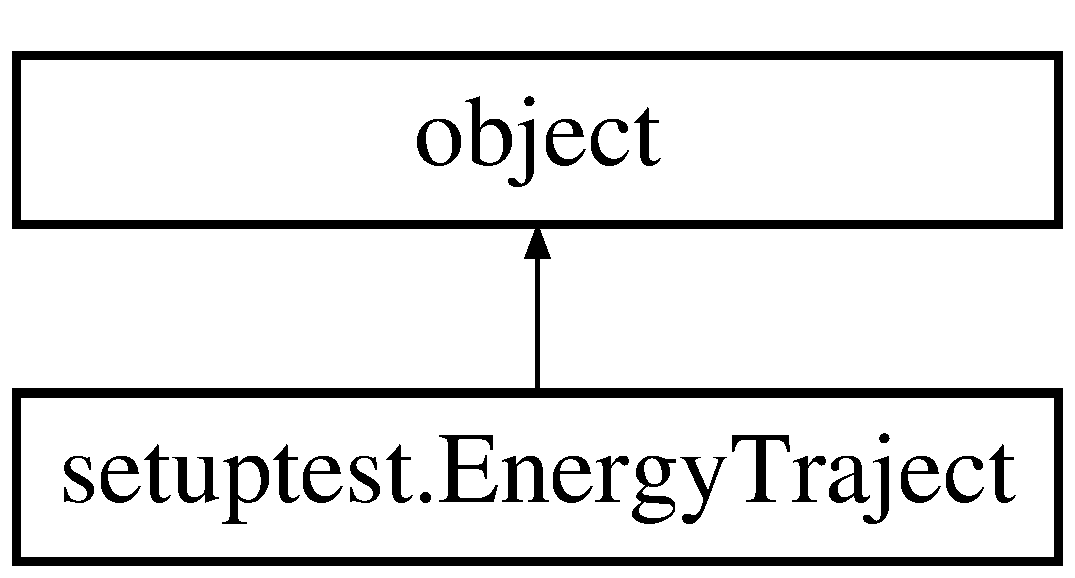
\includegraphics[height=2.000000cm]{classsetuptest_1_1_energy_traject}
\end{center}
\end{figure}
\subsection*{Public Member Functions}
\begin{DoxyCompactItemize}
\item 
def \hyperlink{classsetuptest_1_1_energy_traject_a4d62ec6c7371f2082ab597fd91362135}{\-\_\-\-\_\-init\-\_\-\-\_\-}
\item 
def \hyperlink{classsetuptest_1_1_energy_traject_a48814b9f443420bc62108c1d1041a18c}{add\-Step}
\item 
def \hyperlink{classsetuptest_1_1_energy_traject_afb65af6cd074fb222a0046b807f7afb6}{plot}
\end{DoxyCompactItemize}
\subsection*{Public Attributes}
\begin{DoxyCompactItemize}
\item 
\hyperlink{classsetuptest_1_1_energy_traject_a1b6ed50b43cacca55b035725f61209d4}{steps}
\item 
\hyperlink{classsetuptest_1_1_energy_traject_a42afaf404b3751ccd71132f940cca86f}{energies}
\item 
\hyperlink{classsetuptest_1_1_energy_traject_a1b72e7ba38f589bc5d8da9bdb6a2ab4a}{mc\-Id}
\end{DoxyCompactItemize}


\subsection{Constructor \& Destructor Documentation}
\hypertarget{classsetuptest_1_1_energy_traject_a4d62ec6c7371f2082ab597fd91362135}{\index{setuptest\-::\-Energy\-Traject@{setuptest\-::\-Energy\-Traject}!\-\_\-\-\_\-init\-\_\-\-\_\-@{\-\_\-\-\_\-init\-\_\-\-\_\-}}
\index{\-\_\-\-\_\-init\-\_\-\-\_\-@{\-\_\-\-\_\-init\-\_\-\-\_\-}!setuptest::EnergyTraject@{setuptest\-::\-Energy\-Traject}}
\subsubsection[{\-\_\-\-\_\-init\-\_\-\-\_\-}]{\setlength{\rightskip}{0pt plus 5cm}def setuptest.\-Energy\-Traject.\-\_\-\-\_\-init\-\_\-\-\_\- (
\begin{DoxyParamCaption}
\item[{}]{self}
\end{DoxyParamCaption}
)}}\label{classsetuptest_1_1_energy_traject_a4d62ec6c7371f2082ab597fd91362135}


\subsection{Member Function Documentation}
\hypertarget{classsetuptest_1_1_energy_traject_a48814b9f443420bc62108c1d1041a18c}{\index{setuptest\-::\-Energy\-Traject@{setuptest\-::\-Energy\-Traject}!add\-Step@{add\-Step}}
\index{add\-Step@{add\-Step}!setuptest::EnergyTraject@{setuptest\-::\-Energy\-Traject}}
\subsubsection[{add\-Step}]{\setlength{\rightskip}{0pt plus 5cm}def setuptest.\-Energy\-Traject.\-add\-Step (
\begin{DoxyParamCaption}
\item[{}]{self, }
\item[{}]{each\-Line}
\end{DoxyParamCaption}
)}}\label{classsetuptest_1_1_energy_traject_a48814b9f443420bc62108c1d1041a18c}
\hypertarget{classsetuptest_1_1_energy_traject_afb65af6cd074fb222a0046b807f7afb6}{\index{setuptest\-::\-Energy\-Traject@{setuptest\-::\-Energy\-Traject}!plot@{plot}}
\index{plot@{plot}!setuptest::EnergyTraject@{setuptest\-::\-Energy\-Traject}}
\subsubsection[{plot}]{\setlength{\rightskip}{0pt plus 5cm}def setuptest.\-Energy\-Traject.\-plot (
\begin{DoxyParamCaption}
\item[{}]{self}
\end{DoxyParamCaption}
)}}\label{classsetuptest_1_1_energy_traject_afb65af6cd074fb222a0046b807f7afb6}


\subsection{Member Data Documentation}
\hypertarget{classsetuptest_1_1_energy_traject_a42afaf404b3751ccd71132f940cca86f}{\index{setuptest\-::\-Energy\-Traject@{setuptest\-::\-Energy\-Traject}!energies@{energies}}
\index{energies@{energies}!setuptest::EnergyTraject@{setuptest\-::\-Energy\-Traject}}
\subsubsection[{energies}]{\setlength{\rightskip}{0pt plus 5cm}setuptest.\-Energy\-Traject.\-energies}}\label{classsetuptest_1_1_energy_traject_a42afaf404b3751ccd71132f940cca86f}
\hypertarget{classsetuptest_1_1_energy_traject_a1b72e7ba38f589bc5d8da9bdb6a2ab4a}{\index{setuptest\-::\-Energy\-Traject@{setuptest\-::\-Energy\-Traject}!mc\-Id@{mc\-Id}}
\index{mc\-Id@{mc\-Id}!setuptest::EnergyTraject@{setuptest\-::\-Energy\-Traject}}
\subsubsection[{mc\-Id}]{\setlength{\rightskip}{0pt plus 5cm}setuptest.\-Energy\-Traject.\-mc\-Id}}\label{classsetuptest_1_1_energy_traject_a1b72e7ba38f589bc5d8da9bdb6a2ab4a}
\hypertarget{classsetuptest_1_1_energy_traject_a1b6ed50b43cacca55b035725f61209d4}{\index{setuptest\-::\-Energy\-Traject@{setuptest\-::\-Energy\-Traject}!steps@{steps}}
\index{steps@{steps}!setuptest::EnergyTraject@{setuptest\-::\-Energy\-Traject}}
\subsubsection[{steps}]{\setlength{\rightskip}{0pt plus 5cm}setuptest.\-Energy\-Traject.\-steps}}\label{classsetuptest_1_1_energy_traject_a1b6ed50b43cacca55b035725f61209d4}


The documentation for this class was generated from the following file\-:\begin{DoxyCompactItemize}
\item 
src/scripts/old/\hyperlink{setuptest_8py}{setuptest.\-py}\end{DoxyCompactItemize}

\hypertarget{classatom__hbond_1_1_hbond}{\section{atom\-\_\-hbond.\-Hbond Class Reference}
\label{classatom__hbond_1_1_hbond}\index{atom\-\_\-hbond.\-Hbond@{atom\-\_\-hbond.\-Hbond}}
}
Inheritance diagram for atom\-\_\-hbond.\-Hbond\-:\begin{figure}[H]
\begin{center}
\leavevmode
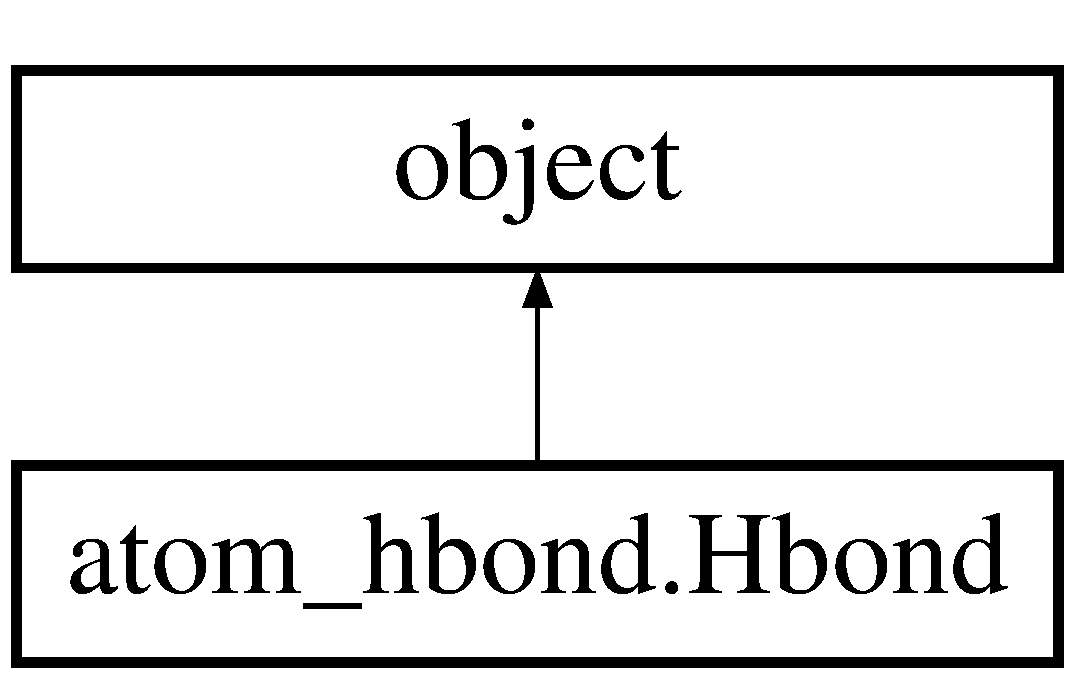
\includegraphics[height=2.000000cm]{classatom__hbond_1_1_hbond}
\end{center}
\end{figure}
\subsection*{Public Member Functions}
\begin{DoxyCompactItemize}
\item 
def \hyperlink{classatom__hbond_1_1_hbond_a8aa7838bbdab8ff6a95df2f2251b9ad5}{\-\_\-\-\_\-init\-\_\-\-\_\-}
\item 
def \hyperlink{classatom__hbond_1_1_hbond_a18151de3db93d22fc62495353e6b1e98}{init\-From\-Line}
\item 
def \hyperlink{classatom__hbond_1_1_hbond_a693582d9198e224eebac628cb8ea5401}{convert\-To\-Res\-Edge}
\item 
def \hyperlink{classatom__hbond_1_1_hbond_a68014f266ecb935af0ed8285c70492f4}{convert\-To\-Res\-Nodes}
\end{DoxyCompactItemize}
\subsection*{Static Public Member Functions}
\begin{DoxyCompactItemize}
\item 
def \hyperlink{classatom__hbond_1_1_hbond_a4e3baeacf725355da76613310b7f0d7f}{conf\-To\-Res}
\end{DoxyCompactItemize}
\subsection*{Public Attributes}
\begin{DoxyCompactItemize}
\item 
\hyperlink{classatom__hbond_1_1_hbond_a5db6b3701d1056d7fb55f891fae5795e}{donor\-Conf}
\item 
\hyperlink{classatom__hbond_1_1_hbond_ad30074a37c7d9d1a7c86a1f3f1d801f9}{donor\-Atom}
\item 
\hyperlink{classatom__hbond_1_1_hbond_afe82776aaf2520c71a04569bd1eb725c}{h\-Atom}
\item 
\hyperlink{classatom__hbond_1_1_hbond_ae6b42002ad388addcc7207184319d00f}{acceptor\-Conf}
\item 
\hyperlink{classatom__hbond_1_1_hbond_a322a0788fabbf71a00bb046bd243a311}{acceptor\-Atom}
\item 
\hyperlink{classatom__hbond_1_1_hbond_a6d6a047e06b0c3ddc4fe79afe7c20aaa}{dist}
\item 
\hyperlink{classatom__hbond_1_1_hbond_a344f4c15bb7233cbee96fd5223983959}{angle}
\item 
\hyperlink{classatom__hbond_1_1_hbond_a742249524df51f1444f2e807f2666347}{donor\-Res}
\item 
\hyperlink{classatom__hbond_1_1_hbond_a49f4560f941edde37b1b4600b8a8fc79}{acceptor\-Res}
\end{DoxyCompactItemize}


\subsection{Constructor \& Destructor Documentation}
\hypertarget{classatom__hbond_1_1_hbond_a8aa7838bbdab8ff6a95df2f2251b9ad5}{\index{atom\-\_\-hbond\-::\-Hbond@{atom\-\_\-hbond\-::\-Hbond}!\-\_\-\-\_\-init\-\_\-\-\_\-@{\-\_\-\-\_\-init\-\_\-\-\_\-}}
\index{\-\_\-\-\_\-init\-\_\-\-\_\-@{\-\_\-\-\_\-init\-\_\-\-\_\-}!atom_hbond::Hbond@{atom\-\_\-hbond\-::\-Hbond}}
\subsubsection[{\-\_\-\-\_\-init\-\_\-\-\_\-}]{\setlength{\rightskip}{0pt plus 5cm}def atom\-\_\-hbond.\-Hbond.\-\_\-\-\_\-init\-\_\-\-\_\- (
\begin{DoxyParamCaption}
\item[{}]{self, }
\item[{}]{donor\-Conf = {\ttfamily \char`\"{}\char`\"{}}, }
\item[{}]{donor\-Atom = {\ttfamily \char`\"{}\char`\"{}}, }
\item[{}]{h\-Atom = {\ttfamily \char`\"{}\char`\"{}}, }
\item[{}]{acceptor\-Conf = {\ttfamily \char`\"{}\char`\"{}}, }
\item[{}]{acceptor\-Atom = {\ttfamily \char`\"{}\char`\"{}}, }
\item[{}]{dist = {\ttfamily 0.0}, }
\item[{}]{angle = {\ttfamily 0}}
\end{DoxyParamCaption}
)}}\label{classatom__hbond_1_1_hbond_a8aa7838bbdab8ff6a95df2f2251b9ad5}


\subsection{Member Function Documentation}
\hypertarget{classatom__hbond_1_1_hbond_a4e3baeacf725355da76613310b7f0d7f}{\index{atom\-\_\-hbond\-::\-Hbond@{atom\-\_\-hbond\-::\-Hbond}!conf\-To\-Res@{conf\-To\-Res}}
\index{conf\-To\-Res@{conf\-To\-Res}!atom_hbond::Hbond@{atom\-\_\-hbond\-::\-Hbond}}
\subsubsection[{conf\-To\-Res}]{\setlength{\rightskip}{0pt plus 5cm}def atom\-\_\-hbond.\-Hbond.\-conf\-To\-Res (
\begin{DoxyParamCaption}
\item[{}]{conf\-Name}
\end{DoxyParamCaption}
)\hspace{0.3cm}{\ttfamily [static]}}}\label{classatom__hbond_1_1_hbond_a4e3baeacf725355da76613310b7f0d7f}
\hypertarget{classatom__hbond_1_1_hbond_a693582d9198e224eebac628cb8ea5401}{\index{atom\-\_\-hbond\-::\-Hbond@{atom\-\_\-hbond\-::\-Hbond}!convert\-To\-Res\-Edge@{convert\-To\-Res\-Edge}}
\index{convert\-To\-Res\-Edge@{convert\-To\-Res\-Edge}!atom_hbond::Hbond@{atom\-\_\-hbond\-::\-Hbond}}
\subsubsection[{convert\-To\-Res\-Edge}]{\setlength{\rightskip}{0pt plus 5cm}def atom\-\_\-hbond.\-Hbond.\-convert\-To\-Res\-Edge (
\begin{DoxyParamCaption}
\item[{}]{self}
\end{DoxyParamCaption}
)}}\label{classatom__hbond_1_1_hbond_a693582d9198e224eebac628cb8ea5401}
\hypertarget{classatom__hbond_1_1_hbond_a68014f266ecb935af0ed8285c70492f4}{\index{atom\-\_\-hbond\-::\-Hbond@{atom\-\_\-hbond\-::\-Hbond}!convert\-To\-Res\-Nodes@{convert\-To\-Res\-Nodes}}
\index{convert\-To\-Res\-Nodes@{convert\-To\-Res\-Nodes}!atom_hbond::Hbond@{atom\-\_\-hbond\-::\-Hbond}}
\subsubsection[{convert\-To\-Res\-Nodes}]{\setlength{\rightskip}{0pt plus 5cm}def atom\-\_\-hbond.\-Hbond.\-convert\-To\-Res\-Nodes (
\begin{DoxyParamCaption}
\item[{}]{self}
\end{DoxyParamCaption}
)}}\label{classatom__hbond_1_1_hbond_a68014f266ecb935af0ed8285c70492f4}
\hypertarget{classatom__hbond_1_1_hbond_a18151de3db93d22fc62495353e6b1e98}{\index{atom\-\_\-hbond\-::\-Hbond@{atom\-\_\-hbond\-::\-Hbond}!init\-From\-Line@{init\-From\-Line}}
\index{init\-From\-Line@{init\-From\-Line}!atom_hbond::Hbond@{atom\-\_\-hbond\-::\-Hbond}}
\subsubsection[{init\-From\-Line}]{\setlength{\rightskip}{0pt plus 5cm}def atom\-\_\-hbond.\-Hbond.\-init\-From\-Line (
\begin{DoxyParamCaption}
\item[{}]{self, }
\item[{}]{line}
\end{DoxyParamCaption}
)}}\label{classatom__hbond_1_1_hbond_a18151de3db93d22fc62495353e6b1e98}


\subsection{Member Data Documentation}
\hypertarget{classatom__hbond_1_1_hbond_a322a0788fabbf71a00bb046bd243a311}{\index{atom\-\_\-hbond\-::\-Hbond@{atom\-\_\-hbond\-::\-Hbond}!acceptor\-Atom@{acceptor\-Atom}}
\index{acceptor\-Atom@{acceptor\-Atom}!atom_hbond::Hbond@{atom\-\_\-hbond\-::\-Hbond}}
\subsubsection[{acceptor\-Atom}]{\setlength{\rightskip}{0pt plus 5cm}atom\-\_\-hbond.\-Hbond.\-acceptor\-Atom}}\label{classatom__hbond_1_1_hbond_a322a0788fabbf71a00bb046bd243a311}
\hypertarget{classatom__hbond_1_1_hbond_ae6b42002ad388addcc7207184319d00f}{\index{atom\-\_\-hbond\-::\-Hbond@{atom\-\_\-hbond\-::\-Hbond}!acceptor\-Conf@{acceptor\-Conf}}
\index{acceptor\-Conf@{acceptor\-Conf}!atom_hbond::Hbond@{atom\-\_\-hbond\-::\-Hbond}}
\subsubsection[{acceptor\-Conf}]{\setlength{\rightskip}{0pt plus 5cm}atom\-\_\-hbond.\-Hbond.\-acceptor\-Conf}}\label{classatom__hbond_1_1_hbond_ae6b42002ad388addcc7207184319d00f}
\hypertarget{classatom__hbond_1_1_hbond_a49f4560f941edde37b1b4600b8a8fc79}{\index{atom\-\_\-hbond\-::\-Hbond@{atom\-\_\-hbond\-::\-Hbond}!acceptor\-Res@{acceptor\-Res}}
\index{acceptor\-Res@{acceptor\-Res}!atom_hbond::Hbond@{atom\-\_\-hbond\-::\-Hbond}}
\subsubsection[{acceptor\-Res}]{\setlength{\rightskip}{0pt plus 5cm}atom\-\_\-hbond.\-Hbond.\-acceptor\-Res}}\label{classatom__hbond_1_1_hbond_a49f4560f941edde37b1b4600b8a8fc79}
\hypertarget{classatom__hbond_1_1_hbond_a344f4c15bb7233cbee96fd5223983959}{\index{atom\-\_\-hbond\-::\-Hbond@{atom\-\_\-hbond\-::\-Hbond}!angle@{angle}}
\index{angle@{angle}!atom_hbond::Hbond@{atom\-\_\-hbond\-::\-Hbond}}
\subsubsection[{angle}]{\setlength{\rightskip}{0pt plus 5cm}atom\-\_\-hbond.\-Hbond.\-angle}}\label{classatom__hbond_1_1_hbond_a344f4c15bb7233cbee96fd5223983959}
\hypertarget{classatom__hbond_1_1_hbond_a6d6a047e06b0c3ddc4fe79afe7c20aaa}{\index{atom\-\_\-hbond\-::\-Hbond@{atom\-\_\-hbond\-::\-Hbond}!dist@{dist}}
\index{dist@{dist}!atom_hbond::Hbond@{atom\-\_\-hbond\-::\-Hbond}}
\subsubsection[{dist}]{\setlength{\rightskip}{0pt plus 5cm}atom\-\_\-hbond.\-Hbond.\-dist}}\label{classatom__hbond_1_1_hbond_a6d6a047e06b0c3ddc4fe79afe7c20aaa}
\hypertarget{classatom__hbond_1_1_hbond_ad30074a37c7d9d1a7c86a1f3f1d801f9}{\index{atom\-\_\-hbond\-::\-Hbond@{atom\-\_\-hbond\-::\-Hbond}!donor\-Atom@{donor\-Atom}}
\index{donor\-Atom@{donor\-Atom}!atom_hbond::Hbond@{atom\-\_\-hbond\-::\-Hbond}}
\subsubsection[{donor\-Atom}]{\setlength{\rightskip}{0pt plus 5cm}atom\-\_\-hbond.\-Hbond.\-donor\-Atom}}\label{classatom__hbond_1_1_hbond_ad30074a37c7d9d1a7c86a1f3f1d801f9}
\hypertarget{classatom__hbond_1_1_hbond_a5db6b3701d1056d7fb55f891fae5795e}{\index{atom\-\_\-hbond\-::\-Hbond@{atom\-\_\-hbond\-::\-Hbond}!donor\-Conf@{donor\-Conf}}
\index{donor\-Conf@{donor\-Conf}!atom_hbond::Hbond@{atom\-\_\-hbond\-::\-Hbond}}
\subsubsection[{donor\-Conf}]{\setlength{\rightskip}{0pt plus 5cm}atom\-\_\-hbond.\-Hbond.\-donor\-Conf}}\label{classatom__hbond_1_1_hbond_a5db6b3701d1056d7fb55f891fae5795e}
\hypertarget{classatom__hbond_1_1_hbond_a742249524df51f1444f2e807f2666347}{\index{atom\-\_\-hbond\-::\-Hbond@{atom\-\_\-hbond\-::\-Hbond}!donor\-Res@{donor\-Res}}
\index{donor\-Res@{donor\-Res}!atom_hbond::Hbond@{atom\-\_\-hbond\-::\-Hbond}}
\subsubsection[{donor\-Res}]{\setlength{\rightskip}{0pt plus 5cm}atom\-\_\-hbond.\-Hbond.\-donor\-Res}}\label{classatom__hbond_1_1_hbond_a742249524df51f1444f2e807f2666347}
\hypertarget{classatom__hbond_1_1_hbond_afe82776aaf2520c71a04569bd1eb725c}{\index{atom\-\_\-hbond\-::\-Hbond@{atom\-\_\-hbond\-::\-Hbond}!h\-Atom@{h\-Atom}}
\index{h\-Atom@{h\-Atom}!atom_hbond::Hbond@{atom\-\_\-hbond\-::\-Hbond}}
\subsubsection[{h\-Atom}]{\setlength{\rightskip}{0pt plus 5cm}atom\-\_\-hbond.\-Hbond.\-h\-Atom}}\label{classatom__hbond_1_1_hbond_afe82776aaf2520c71a04569bd1eb725c}


The documentation for this class was generated from the following file\-:\begin{DoxyCompactItemize}
\item 
src/scripts/hb\-\_\-connection/\hyperlink{atom__hbond_8py}{atom\-\_\-hbond.\-py}\end{DoxyCompactItemize}

\hypertarget{classarg82__conn_1_1_hb_path}{\section{arg82\-\_\-conn.\-Hb\-Path Class Reference}
\label{classarg82__conn_1_1_hb_path}\index{arg82\-\_\-conn.\-Hb\-Path@{arg82\-\_\-conn.\-Hb\-Path}}
}
Inheritance diagram for arg82\-\_\-conn.\-Hb\-Path\-:\begin{figure}[H]
\begin{center}
\leavevmode
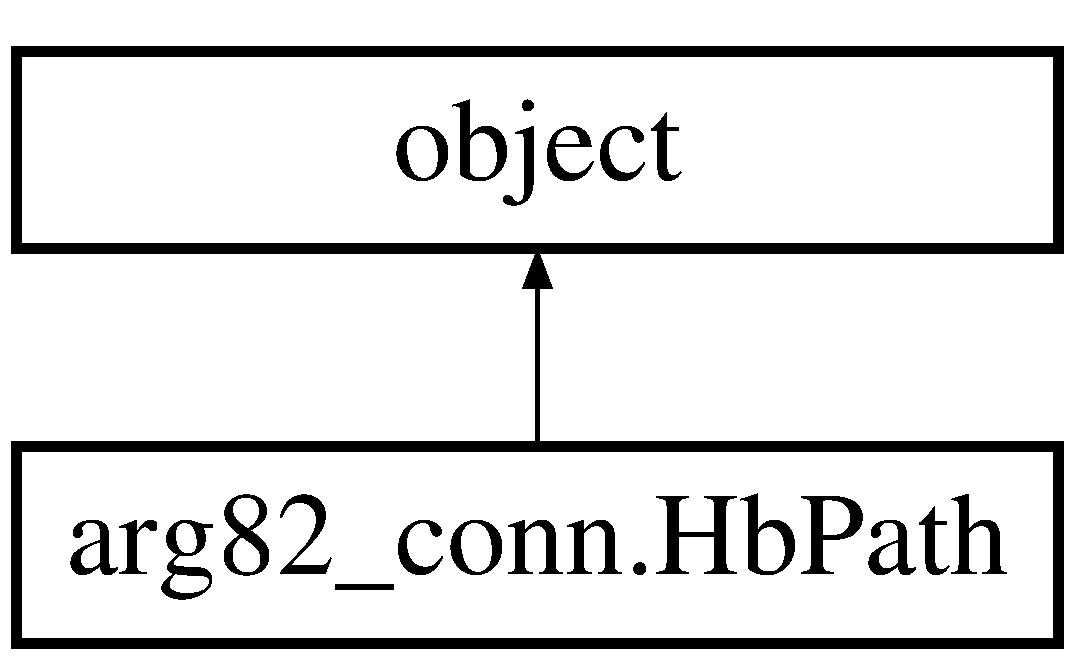
\includegraphics[height=2.000000cm]{classarg82__conn_1_1_hb_path}
\end{center}
\end{figure}
\subsection*{Public Member Functions}
\begin{DoxyCompactItemize}
\item 
def \hyperlink{classarg82__conn_1_1_hb_path_a58bb4c090c043e019974cd3464ee3150}{\-\_\-\-\_\-init\-\_\-\-\_\-}
\item 
def \hyperlink{classarg82__conn_1_1_hb_path_a14e48479493b0d9c3476375d2ca13f9c}{load\-Path\-Info}
\begin{DoxyCompactList}\small\item\em Get the key residues in the pathway, and their possible protonation states, and the initial state. \end{DoxyCompactList}\item 
def \hyperlink{classarg82__conn_1_1_hb_path_a3dcd2c4ea4f9158095b2fcbf03345a26}{get\-All\-Hop\-Sequences}
\item 
def \hyperlink{classarg82__conn_1_1_hb_path_a784881af9af8c34a5f444d6e840238c1}{load\-\_\-intermediates}
\begin{DoxyCompactList}\small\item\em Load energies of protonation states from intermediates.\-txt. \end{DoxyCompactList}\item 
def \hyperlink{classarg82__conn_1_1_hb_path_a41dc0009b9723d4d31354bb830644b92}{load\-\_\-hop\-Sequences}
\begin{DoxyCompactList}\small\item\em Load all the possible hop sequences from hop\-Sequences.\-txt file. \end{DoxyCompactList}\item 
def \hyperlink{classarg82__conn_1_1_hb_path_a7376dc922ba91162d573fe83856d9d58}{load\-\_\-calculated\-\_\-path}
\end{DoxyCompactItemize}
\subsection*{Public Attributes}
\begin{DoxyCompactItemize}
\item 
\hyperlink{classarg82__conn_1_1_hb_path_aac4d722df28508785039f5272eb99dcf}{key\-Residues}
\item 
\hyperlink{classarg82__conn_1_1_hb_path_a05571020ca98f5dcc62546f6cc7b3cfa}{possible\-Protonations}
\item 
\hyperlink{classarg82__conn_1_1_hb_path_a9590e6f31273ef08d205c8a9ecd3d848}{initial\-State}
\item 
\hyperlink{classarg82__conn_1_1_hb_path_ae8eab29c776e119ec7010fb549651a67}{n\-Residues}
\item 
\hyperlink{classarg82__conn_1_1_hb_path_ae2d2d12e2a9c3ff2abaa6b73c6117bcd}{hop\-Sequences}
\item 
\hyperlink{classarg82__conn_1_1_hb_path_a703ccb2cd6fb30f1fdec066071abe05c}{protonation\-States}
\end{DoxyCompactItemize}


\subsection{Constructor \& Destructor Documentation}
\hypertarget{classarg82__conn_1_1_hb_path_a58bb4c090c043e019974cd3464ee3150}{\index{arg82\-\_\-conn\-::\-Hb\-Path@{arg82\-\_\-conn\-::\-Hb\-Path}!\-\_\-\-\_\-init\-\_\-\-\_\-@{\-\_\-\-\_\-init\-\_\-\-\_\-}}
\index{\-\_\-\-\_\-init\-\_\-\-\_\-@{\-\_\-\-\_\-init\-\_\-\-\_\-}!arg82_conn::HbPath@{arg82\-\_\-conn\-::\-Hb\-Path}}
\subsubsection[{\-\_\-\-\_\-init\-\_\-\-\_\-}]{\setlength{\rightskip}{0pt plus 5cm}def arg82\-\_\-conn.\-Hb\-Path.\-\_\-\-\_\-init\-\_\-\-\_\- (
\begin{DoxyParamCaption}
\item[{}]{self}
\end{DoxyParamCaption}
)}}\label{classarg82__conn_1_1_hb_path_a58bb4c090c043e019974cd3464ee3150}


\subsection{Member Function Documentation}
\hypertarget{classarg82__conn_1_1_hb_path_a3dcd2c4ea4f9158095b2fcbf03345a26}{\index{arg82\-\_\-conn\-::\-Hb\-Path@{arg82\-\_\-conn\-::\-Hb\-Path}!get\-All\-Hop\-Sequences@{get\-All\-Hop\-Sequences}}
\index{get\-All\-Hop\-Sequences@{get\-All\-Hop\-Sequences}!arg82_conn::HbPath@{arg82\-\_\-conn\-::\-Hb\-Path}}
\subsubsection[{get\-All\-Hop\-Sequences}]{\setlength{\rightskip}{0pt plus 5cm}def arg82\-\_\-conn.\-Hb\-Path.\-get\-All\-Hop\-Sequences (
\begin{DoxyParamCaption}
\item[{}]{self}
\end{DoxyParamCaption}
)}}\label{classarg82__conn_1_1_hb_path_a3dcd2c4ea4f9158095b2fcbf03345a26}
\hypertarget{classarg82__conn_1_1_hb_path_a7376dc922ba91162d573fe83856d9d58}{\index{arg82\-\_\-conn\-::\-Hb\-Path@{arg82\-\_\-conn\-::\-Hb\-Path}!load\-\_\-calculated\-\_\-path@{load\-\_\-calculated\-\_\-path}}
\index{load\-\_\-calculated\-\_\-path@{load\-\_\-calculated\-\_\-path}!arg82_conn::HbPath@{arg82\-\_\-conn\-::\-Hb\-Path}}
\subsubsection[{load\-\_\-calculated\-\_\-path}]{\setlength{\rightskip}{0pt plus 5cm}def arg82\-\_\-conn.\-Hb\-Path.\-load\-\_\-calculated\-\_\-path (
\begin{DoxyParamCaption}
\item[{}]{self, }
\item[{}]{pathinfo\-File = {\ttfamily \char`\"{}pathinfo.txt\char`\"{}}, }
\item[{}]{intermediates\-File = {\ttfamily \char`\"{}intermediates.txt\char`\"{}}, }
\item[{}]{hop\-Sequences\-File = {\ttfamily \char`\"{}hopSequences.txt\char`\"{}}}
\end{DoxyParamCaption}
)}}\label{classarg82__conn_1_1_hb_path_a7376dc922ba91162d573fe83856d9d58}
\hypertarget{classarg82__conn_1_1_hb_path_a41dc0009b9723d4d31354bb830644b92}{\index{arg82\-\_\-conn\-::\-Hb\-Path@{arg82\-\_\-conn\-::\-Hb\-Path}!load\-\_\-hop\-Sequences@{load\-\_\-hop\-Sequences}}
\index{load\-\_\-hop\-Sequences@{load\-\_\-hop\-Sequences}!arg82_conn::HbPath@{arg82\-\_\-conn\-::\-Hb\-Path}}
\subsubsection[{load\-\_\-hop\-Sequences}]{\setlength{\rightskip}{0pt plus 5cm}def arg82\-\_\-conn.\-Hb\-Path.\-load\-\_\-hop\-Sequences (
\begin{DoxyParamCaption}
\item[{}]{self, }
\item[{}]{hop\-Sequences\-File = {\ttfamily \char`\"{}hopSequences.txt\char`\"{}}}
\end{DoxyParamCaption}
)}}\label{classarg82__conn_1_1_hb_path_a41dc0009b9723d4d31354bb830644b92}


Load all the possible hop sequences from hop\-Sequences.\-txt file. 

Energies of intermediates should have been loaded from intermediates.\-txt first. It will not load the intermediates again in this file. \hypertarget{classarg82__conn_1_1_hb_path_a784881af9af8c34a5f444d6e840238c1}{\index{arg82\-\_\-conn\-::\-Hb\-Path@{arg82\-\_\-conn\-::\-Hb\-Path}!load\-\_\-intermediates@{load\-\_\-intermediates}}
\index{load\-\_\-intermediates@{load\-\_\-intermediates}!arg82_conn::HbPath@{arg82\-\_\-conn\-::\-Hb\-Path}}
\subsubsection[{load\-\_\-intermediates}]{\setlength{\rightskip}{0pt plus 5cm}def arg82\-\_\-conn.\-Hb\-Path.\-load\-\_\-intermediates (
\begin{DoxyParamCaption}
\item[{}]{self, }
\item[{}]{intermediates\-File = {\ttfamily \char`\"{}intermediates.txt\char`\"{}}}
\end{DoxyParamCaption}
)}}\label{classarg82__conn_1_1_hb_path_a784881af9af8c34a5f444d6e840238c1}


Load energies of protonation states from intermediates.\-txt. 

\hypertarget{classarg82__conn_1_1_hb_path_a14e48479493b0d9c3476375d2ca13f9c}{\index{arg82\-\_\-conn\-::\-Hb\-Path@{arg82\-\_\-conn\-::\-Hb\-Path}!load\-Path\-Info@{load\-Path\-Info}}
\index{load\-Path\-Info@{load\-Path\-Info}!arg82_conn::HbPath@{arg82\-\_\-conn\-::\-Hb\-Path}}
\subsubsection[{load\-Path\-Info}]{\setlength{\rightskip}{0pt plus 5cm}def arg82\-\_\-conn.\-Hb\-Path.\-load\-Path\-Info (
\begin{DoxyParamCaption}
\item[{}]{self, }
\item[{}]{f\-Name = {\ttfamily {\bf P\-A\-T\-H\-\_\-\-I\-N\-F\-O\-\_\-\-F\-I\-L\-E}}}
\end{DoxyParamCaption}
)}}\label{classarg82__conn_1_1_hb_path_a14e48479493b0d9c3476375d2ca13f9c}


Get the key residues in the pathway, and their possible protonation states, and the initial state. 

Return an object of class Path\-Config containing this information. \begin{DoxyVerb}    The file format should be like this:
    ASPA0085  -1  0
    HOHA0402  -1  0  1
    HOHA0406  -1  0  1
    ARGA0082   0  1
    HOHA0403  -1  0  1
    GLUA0194  -1  0
     0 0 0 1 0 -1

     The last line is the initial state.
     The other lines give the name of the residues, following all their possible protonation states\end{DoxyVerb}
 

\subsection{Member Data Documentation}
\hypertarget{classarg82__conn_1_1_hb_path_ae2d2d12e2a9c3ff2abaa6b73c6117bcd}{\index{arg82\-\_\-conn\-::\-Hb\-Path@{arg82\-\_\-conn\-::\-Hb\-Path}!hop\-Sequences@{hop\-Sequences}}
\index{hop\-Sequences@{hop\-Sequences}!arg82_conn::HbPath@{arg82\-\_\-conn\-::\-Hb\-Path}}
\subsubsection[{hop\-Sequences}]{\setlength{\rightskip}{0pt plus 5cm}arg82\-\_\-conn.\-Hb\-Path.\-hop\-Sequences}}\label{classarg82__conn_1_1_hb_path_ae2d2d12e2a9c3ff2abaa6b73c6117bcd}
\hypertarget{classarg82__conn_1_1_hb_path_a9590e6f31273ef08d205c8a9ecd3d848}{\index{arg82\-\_\-conn\-::\-Hb\-Path@{arg82\-\_\-conn\-::\-Hb\-Path}!initial\-State@{initial\-State}}
\index{initial\-State@{initial\-State}!arg82_conn::HbPath@{arg82\-\_\-conn\-::\-Hb\-Path}}
\subsubsection[{initial\-State}]{\setlength{\rightskip}{0pt plus 5cm}arg82\-\_\-conn.\-Hb\-Path.\-initial\-State}}\label{classarg82__conn_1_1_hb_path_a9590e6f31273ef08d205c8a9ecd3d848}
\hypertarget{classarg82__conn_1_1_hb_path_aac4d722df28508785039f5272eb99dcf}{\index{arg82\-\_\-conn\-::\-Hb\-Path@{arg82\-\_\-conn\-::\-Hb\-Path}!key\-Residues@{key\-Residues}}
\index{key\-Residues@{key\-Residues}!arg82_conn::HbPath@{arg82\-\_\-conn\-::\-Hb\-Path}}
\subsubsection[{key\-Residues}]{\setlength{\rightskip}{0pt plus 5cm}arg82\-\_\-conn.\-Hb\-Path.\-key\-Residues}}\label{classarg82__conn_1_1_hb_path_aac4d722df28508785039f5272eb99dcf}
\hypertarget{classarg82__conn_1_1_hb_path_ae8eab29c776e119ec7010fb549651a67}{\index{arg82\-\_\-conn\-::\-Hb\-Path@{arg82\-\_\-conn\-::\-Hb\-Path}!n\-Residues@{n\-Residues}}
\index{n\-Residues@{n\-Residues}!arg82_conn::HbPath@{arg82\-\_\-conn\-::\-Hb\-Path}}
\subsubsection[{n\-Residues}]{\setlength{\rightskip}{0pt plus 5cm}arg82\-\_\-conn.\-Hb\-Path.\-n\-Residues}}\label{classarg82__conn_1_1_hb_path_ae8eab29c776e119ec7010fb549651a67}
\hypertarget{classarg82__conn_1_1_hb_path_a05571020ca98f5dcc62546f6cc7b3cfa}{\index{arg82\-\_\-conn\-::\-Hb\-Path@{arg82\-\_\-conn\-::\-Hb\-Path}!possible\-Protonations@{possible\-Protonations}}
\index{possible\-Protonations@{possible\-Protonations}!arg82_conn::HbPath@{arg82\-\_\-conn\-::\-Hb\-Path}}
\subsubsection[{possible\-Protonations}]{\setlength{\rightskip}{0pt plus 5cm}arg82\-\_\-conn.\-Hb\-Path.\-possible\-Protonations}}\label{classarg82__conn_1_1_hb_path_a05571020ca98f5dcc62546f6cc7b3cfa}
\hypertarget{classarg82__conn_1_1_hb_path_a703ccb2cd6fb30f1fdec066071abe05c}{\index{arg82\-\_\-conn\-::\-Hb\-Path@{arg82\-\_\-conn\-::\-Hb\-Path}!protonation\-States@{protonation\-States}}
\index{protonation\-States@{protonation\-States}!arg82_conn::HbPath@{arg82\-\_\-conn\-::\-Hb\-Path}}
\subsubsection[{protonation\-States}]{\setlength{\rightskip}{0pt plus 5cm}arg82\-\_\-conn.\-Hb\-Path.\-protonation\-States}}\label{classarg82__conn_1_1_hb_path_a703ccb2cd6fb30f1fdec066071abe05c}


The documentation for this class was generated from the following file\-:\begin{DoxyCompactItemize}
\item 
src/scripts/hb\-\_\-connection/\hyperlink{arg82__conn_8py}{arg82\-\_\-conn.\-py}\end{DoxyCompactItemize}

\hypertarget{classhbnet_1_1_hb_path}{\section{hbnet.\-Hb\-Path Class Reference}
\label{classhbnet_1_1_hb_path}\index{hbnet.\-Hb\-Path@{hbnet.\-Hb\-Path}}
}
Inheritance diagram for hbnet.\-Hb\-Path\-:\begin{figure}[H]
\begin{center}
\leavevmode
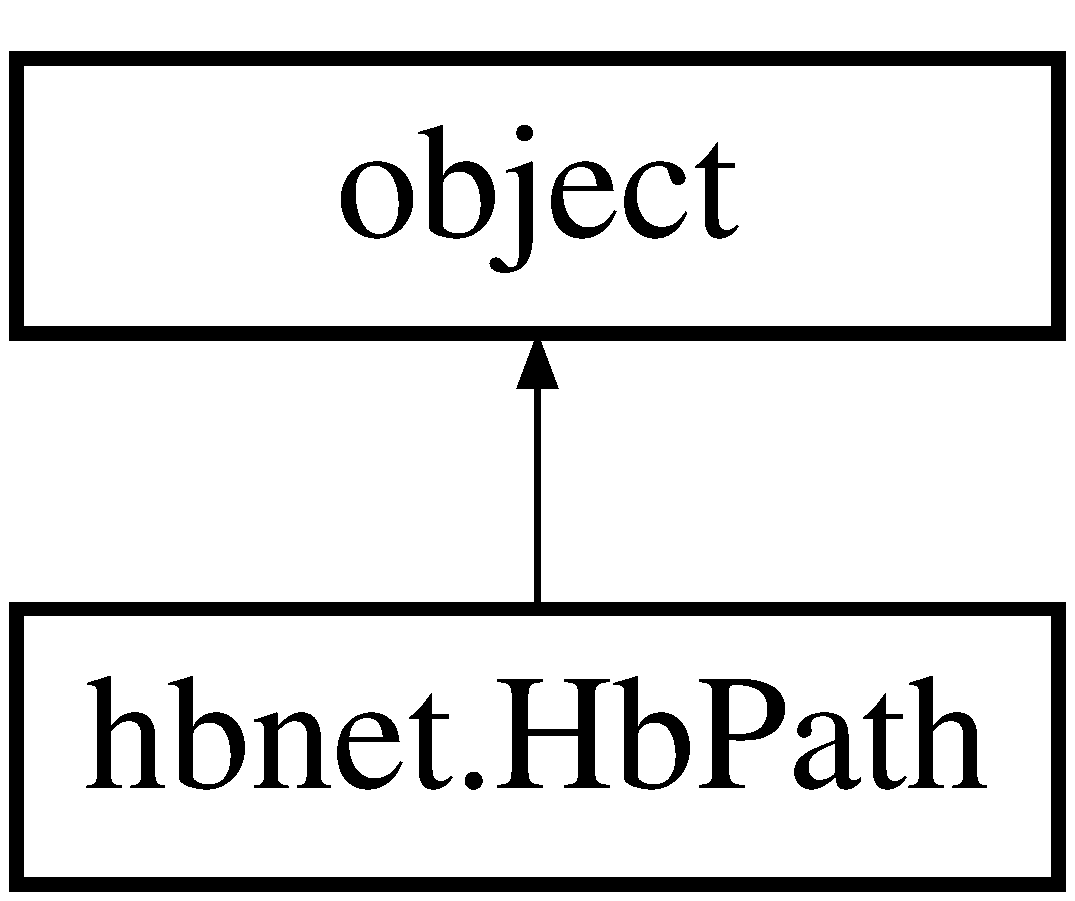
\includegraphics[height=2.000000cm]{classhbnet_1_1_hb_path}
\end{center}
\end{figure}
\subsection*{Public Member Functions}
\begin{DoxyCompactItemize}
\item 
def \hyperlink{classhbnet_1_1_hb_path_accc0aea55bbab3dcff88bc008f9f164e}{\-\_\-\-\_\-init\-\_\-\-\_\-}
\item 
def \hyperlink{classhbnet_1_1_hb_path_a27380bf0f935a0178f5218113f13cc08}{load\-Path\-Info}
\begin{DoxyCompactList}\small\item\em Get the key residues in the pathway, and their possible protonation states, and the initial state. \end{DoxyCompactList}\item 
def \hyperlink{classhbnet_1_1_hb_path_aabee126deca6cdfe0165c7eca0f4f455}{get\-All\-Hop\-Sequences}
\item 
def \hyperlink{classhbnet_1_1_hb_path_aea7db290b896d2e81df966a14d68b6fe}{load\-\_\-intermediates}
\begin{DoxyCompactList}\small\item\em Load energies of protonation states from intermediates.\-txt. \end{DoxyCompactList}\item 
def \hyperlink{classhbnet_1_1_hb_path_a0ee3abc28d0e7c811abd45a8bae85aef}{load\-\_\-hop\-Sequences}
\begin{DoxyCompactList}\small\item\em Load all the possible hop sequences from hop\-Sequences.\-txt file. \end{DoxyCompactList}\item 
def \hyperlink{classhbnet_1_1_hb_path_a15a0c1834be05a45b040f101f6020440}{load\-\_\-calculated\-\_\-path}
\end{DoxyCompactItemize}
\subsection*{Public Attributes}
\begin{DoxyCompactItemize}
\item 
\hyperlink{classhbnet_1_1_hb_path_acadff0bd1e1990b439f50002856daf4a}{key\-Residues}
\item 
\hyperlink{classhbnet_1_1_hb_path_afb0cba5a56b71bee34ab7d21e04182f9}{possible\-Protonations}
\item 
\hyperlink{classhbnet_1_1_hb_path_aa8bdeb3072d6d8aa5cfef98512b2c765}{initial\-State}
\item 
\hyperlink{classhbnet_1_1_hb_path_ab9d8f9c208c0d8001a676fa94db0c1e4}{n\-Residues}
\item 
\hyperlink{classhbnet_1_1_hb_path_ad4ad6ae5b069a3b4d7b275e7ce2c2b08}{hop\-Sequences}
\item 
\hyperlink{classhbnet_1_1_hb_path_a68abdff4f3379feafefde52a57c63f62}{protonation\-States}
\end{DoxyCompactItemize}


\subsection{Constructor \& Destructor Documentation}
\hypertarget{classhbnet_1_1_hb_path_accc0aea55bbab3dcff88bc008f9f164e}{\index{hbnet\-::\-Hb\-Path@{hbnet\-::\-Hb\-Path}!\-\_\-\-\_\-init\-\_\-\-\_\-@{\-\_\-\-\_\-init\-\_\-\-\_\-}}
\index{\-\_\-\-\_\-init\-\_\-\-\_\-@{\-\_\-\-\_\-init\-\_\-\-\_\-}!hbnet::HbPath@{hbnet\-::\-Hb\-Path}}
\subsubsection[{\-\_\-\-\_\-init\-\_\-\-\_\-}]{\setlength{\rightskip}{0pt plus 5cm}def hbnet.\-Hb\-Path.\-\_\-\-\_\-init\-\_\-\-\_\- (
\begin{DoxyParamCaption}
\item[{}]{self}
\end{DoxyParamCaption}
)}}\label{classhbnet_1_1_hb_path_accc0aea55bbab3dcff88bc008f9f164e}


\subsection{Member Function Documentation}
\hypertarget{classhbnet_1_1_hb_path_aabee126deca6cdfe0165c7eca0f4f455}{\index{hbnet\-::\-Hb\-Path@{hbnet\-::\-Hb\-Path}!get\-All\-Hop\-Sequences@{get\-All\-Hop\-Sequences}}
\index{get\-All\-Hop\-Sequences@{get\-All\-Hop\-Sequences}!hbnet::HbPath@{hbnet\-::\-Hb\-Path}}
\subsubsection[{get\-All\-Hop\-Sequences}]{\setlength{\rightskip}{0pt plus 5cm}def hbnet.\-Hb\-Path.\-get\-All\-Hop\-Sequences (
\begin{DoxyParamCaption}
\item[{}]{self}
\end{DoxyParamCaption}
)}}\label{classhbnet_1_1_hb_path_aabee126deca6cdfe0165c7eca0f4f455}
\hypertarget{classhbnet_1_1_hb_path_a15a0c1834be05a45b040f101f6020440}{\index{hbnet\-::\-Hb\-Path@{hbnet\-::\-Hb\-Path}!load\-\_\-calculated\-\_\-path@{load\-\_\-calculated\-\_\-path}}
\index{load\-\_\-calculated\-\_\-path@{load\-\_\-calculated\-\_\-path}!hbnet::HbPath@{hbnet\-::\-Hb\-Path}}
\subsubsection[{load\-\_\-calculated\-\_\-path}]{\setlength{\rightskip}{0pt plus 5cm}def hbnet.\-Hb\-Path.\-load\-\_\-calculated\-\_\-path (
\begin{DoxyParamCaption}
\item[{}]{self, }
\item[{}]{pathinfo\-File = {\ttfamily \char`\"{}pathinfo.txt\char`\"{}}, }
\item[{}]{intermediates\-File = {\ttfamily \char`\"{}intermediates.txt\char`\"{}}, }
\item[{}]{hop\-Sequences\-File = {\ttfamily \char`\"{}hopSequences.txt\char`\"{}}}
\end{DoxyParamCaption}
)}}\label{classhbnet_1_1_hb_path_a15a0c1834be05a45b040f101f6020440}
\hypertarget{classhbnet_1_1_hb_path_a0ee3abc28d0e7c811abd45a8bae85aef}{\index{hbnet\-::\-Hb\-Path@{hbnet\-::\-Hb\-Path}!load\-\_\-hop\-Sequences@{load\-\_\-hop\-Sequences}}
\index{load\-\_\-hop\-Sequences@{load\-\_\-hop\-Sequences}!hbnet::HbPath@{hbnet\-::\-Hb\-Path}}
\subsubsection[{load\-\_\-hop\-Sequences}]{\setlength{\rightskip}{0pt plus 5cm}def hbnet.\-Hb\-Path.\-load\-\_\-hop\-Sequences (
\begin{DoxyParamCaption}
\item[{}]{self, }
\item[{}]{hop\-Sequences\-File = {\ttfamily \char`\"{}hopSequences.txt\char`\"{}}}
\end{DoxyParamCaption}
)}}\label{classhbnet_1_1_hb_path_a0ee3abc28d0e7c811abd45a8bae85aef}


Load all the possible hop sequences from hop\-Sequences.\-txt file. 

Energies of intermediates should have been loaded from intermediates.\-txt first. It will not load the intermediates again in this file. \hypertarget{classhbnet_1_1_hb_path_aea7db290b896d2e81df966a14d68b6fe}{\index{hbnet\-::\-Hb\-Path@{hbnet\-::\-Hb\-Path}!load\-\_\-intermediates@{load\-\_\-intermediates}}
\index{load\-\_\-intermediates@{load\-\_\-intermediates}!hbnet::HbPath@{hbnet\-::\-Hb\-Path}}
\subsubsection[{load\-\_\-intermediates}]{\setlength{\rightskip}{0pt plus 5cm}def hbnet.\-Hb\-Path.\-load\-\_\-intermediates (
\begin{DoxyParamCaption}
\item[{}]{self, }
\item[{}]{intermediates\-File = {\ttfamily \char`\"{}intermediates.txt\char`\"{}}}
\end{DoxyParamCaption}
)}}\label{classhbnet_1_1_hb_path_aea7db290b896d2e81df966a14d68b6fe}


Load energies of protonation states from intermediates.\-txt. 

\hypertarget{classhbnet_1_1_hb_path_a27380bf0f935a0178f5218113f13cc08}{\index{hbnet\-::\-Hb\-Path@{hbnet\-::\-Hb\-Path}!load\-Path\-Info@{load\-Path\-Info}}
\index{load\-Path\-Info@{load\-Path\-Info}!hbnet::HbPath@{hbnet\-::\-Hb\-Path}}
\subsubsection[{load\-Path\-Info}]{\setlength{\rightskip}{0pt plus 5cm}def hbnet.\-Hb\-Path.\-load\-Path\-Info (
\begin{DoxyParamCaption}
\item[{}]{self, }
\item[{}]{f\-Name = {\ttfamily {\bf P\-A\-T\-H\-\_\-\-I\-N\-F\-O\-\_\-\-F\-I\-L\-E}}}
\end{DoxyParamCaption}
)}}\label{classhbnet_1_1_hb_path_a27380bf0f935a0178f5218113f13cc08}


Get the key residues in the pathway, and their possible protonation states, and the initial state. 

Return an object of class Path\-Config containing this information. \begin{DoxyVerb}    The file format should be like this:
    ASPA0085  -1  0
    HOHA0402  -1  0  1
    HOHA0406  -1  0  1
    ARGA0082   0  1
    HOHA0403  -1  0  1
    GLUA0194  -1  0
     0 0 0 1 0 -1

     The last line is the initial state.
     The other lines give the name of the residues, following all their possible protonation states\end{DoxyVerb}
 

\subsection{Member Data Documentation}
\hypertarget{classhbnet_1_1_hb_path_ad4ad6ae5b069a3b4d7b275e7ce2c2b08}{\index{hbnet\-::\-Hb\-Path@{hbnet\-::\-Hb\-Path}!hop\-Sequences@{hop\-Sequences}}
\index{hop\-Sequences@{hop\-Sequences}!hbnet::HbPath@{hbnet\-::\-Hb\-Path}}
\subsubsection[{hop\-Sequences}]{\setlength{\rightskip}{0pt plus 5cm}hbnet.\-Hb\-Path.\-hop\-Sequences}}\label{classhbnet_1_1_hb_path_ad4ad6ae5b069a3b4d7b275e7ce2c2b08}
\hypertarget{classhbnet_1_1_hb_path_aa8bdeb3072d6d8aa5cfef98512b2c765}{\index{hbnet\-::\-Hb\-Path@{hbnet\-::\-Hb\-Path}!initial\-State@{initial\-State}}
\index{initial\-State@{initial\-State}!hbnet::HbPath@{hbnet\-::\-Hb\-Path}}
\subsubsection[{initial\-State}]{\setlength{\rightskip}{0pt plus 5cm}hbnet.\-Hb\-Path.\-initial\-State}}\label{classhbnet_1_1_hb_path_aa8bdeb3072d6d8aa5cfef98512b2c765}
\hypertarget{classhbnet_1_1_hb_path_acadff0bd1e1990b439f50002856daf4a}{\index{hbnet\-::\-Hb\-Path@{hbnet\-::\-Hb\-Path}!key\-Residues@{key\-Residues}}
\index{key\-Residues@{key\-Residues}!hbnet::HbPath@{hbnet\-::\-Hb\-Path}}
\subsubsection[{key\-Residues}]{\setlength{\rightskip}{0pt plus 5cm}hbnet.\-Hb\-Path.\-key\-Residues}}\label{classhbnet_1_1_hb_path_acadff0bd1e1990b439f50002856daf4a}
\hypertarget{classhbnet_1_1_hb_path_ab9d8f9c208c0d8001a676fa94db0c1e4}{\index{hbnet\-::\-Hb\-Path@{hbnet\-::\-Hb\-Path}!n\-Residues@{n\-Residues}}
\index{n\-Residues@{n\-Residues}!hbnet::HbPath@{hbnet\-::\-Hb\-Path}}
\subsubsection[{n\-Residues}]{\setlength{\rightskip}{0pt plus 5cm}hbnet.\-Hb\-Path.\-n\-Residues}}\label{classhbnet_1_1_hb_path_ab9d8f9c208c0d8001a676fa94db0c1e4}
\hypertarget{classhbnet_1_1_hb_path_afb0cba5a56b71bee34ab7d21e04182f9}{\index{hbnet\-::\-Hb\-Path@{hbnet\-::\-Hb\-Path}!possible\-Protonations@{possible\-Protonations}}
\index{possible\-Protonations@{possible\-Protonations}!hbnet::HbPath@{hbnet\-::\-Hb\-Path}}
\subsubsection[{possible\-Protonations}]{\setlength{\rightskip}{0pt plus 5cm}hbnet.\-Hb\-Path.\-possible\-Protonations}}\label{classhbnet_1_1_hb_path_afb0cba5a56b71bee34ab7d21e04182f9}
\hypertarget{classhbnet_1_1_hb_path_a68abdff4f3379feafefde52a57c63f62}{\index{hbnet\-::\-Hb\-Path@{hbnet\-::\-Hb\-Path}!protonation\-States@{protonation\-States}}
\index{protonation\-States@{protonation\-States}!hbnet::HbPath@{hbnet\-::\-Hb\-Path}}
\subsubsection[{protonation\-States}]{\setlength{\rightskip}{0pt plus 5cm}hbnet.\-Hb\-Path.\-protonation\-States}}\label{classhbnet_1_1_hb_path_a68abdff4f3379feafefde52a57c63f62}


The documentation for this class was generated from the following file\-:\begin{DoxyCompactItemize}
\item 
src/scripts/hb\-\_\-connection/\hyperlink{hbnet_8py}{hbnet.\-py}\end{DoxyCompactItemize}

\hypertarget{classget__path__barrier_1_1_hb_path}{\section{get\-\_\-path\-\_\-barrier.\-Hb\-Path Class Reference}
\label{classget__path__barrier_1_1_hb_path}\index{get\-\_\-path\-\_\-barrier.\-Hb\-Path@{get\-\_\-path\-\_\-barrier.\-Hb\-Path}}
}
Inheritance diagram for get\-\_\-path\-\_\-barrier.\-Hb\-Path\-:\begin{figure}[H]
\begin{center}
\leavevmode
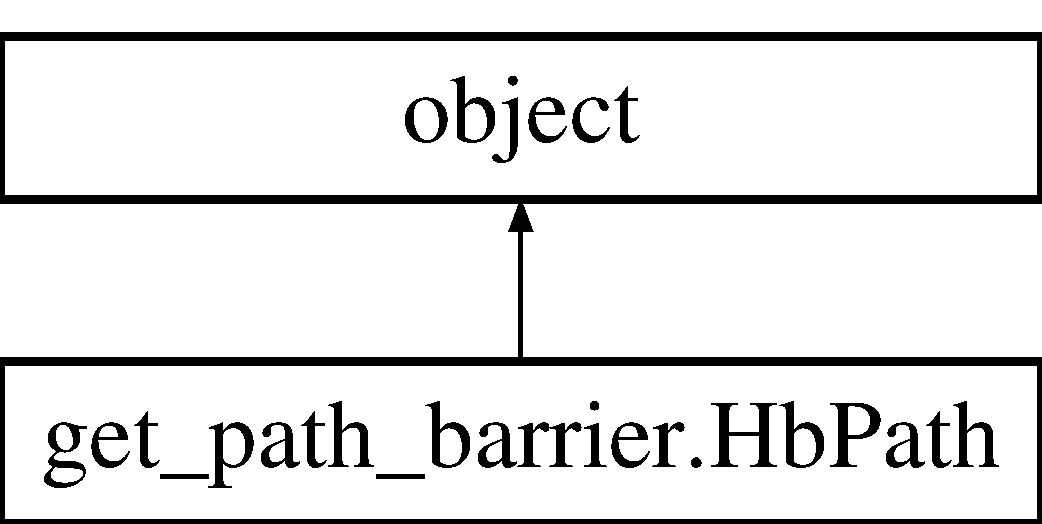
\includegraphics[height=2.000000cm]{classget__path__barrier_1_1_hb_path}
\end{center}
\end{figure}
\subsection*{Public Member Functions}
\begin{DoxyCompactItemize}
\item 
def \hyperlink{classget__path__barrier_1_1_hb_path_ac8526be6c34f93d3991d772e51ac2dd0}{\-\_\-\-\_\-init\-\_\-\-\_\-}
\item 
def \hyperlink{classget__path__barrier_1_1_hb_path_aba025f763752636443417573fc82e941}{load\-Path\-Info}
\begin{DoxyCompactList}\small\item\em Get the key residues in the pathway, and their possible protonation states, and the initial state. \end{DoxyCompactList}\item 
def \hyperlink{classget__path__barrier_1_1_hb_path_a7b689f661b263b4a027559f306b44567}{get\-All\-Hop\-Sequences}
\end{DoxyCompactItemize}
\subsection*{Public Attributes}
\begin{DoxyCompactItemize}
\item 
\hyperlink{classget__path__barrier_1_1_hb_path_af574f30a4a9297c5b798a9f5ab93429c}{key\-Residues}
\item 
\hyperlink{classget__path__barrier_1_1_hb_path_aa3cc8420eaf75f40689de3c1c4ef9143}{possible\-Protonations}
\item 
\hyperlink{classget__path__barrier_1_1_hb_path_acb500e7ef9452b85d3a037ae96b952d3}{initial\-State}
\item 
\hyperlink{classget__path__barrier_1_1_hb_path_abde19f996710977a200bbd380327d992}{n\-Residues}
\item 
\hyperlink{classget__path__barrier_1_1_hb_path_a838cc727a1853ae9dbcda45158c4ff1d}{hop\-Sequences}
\item 
\hyperlink{classget__path__barrier_1_1_hb_path_a232b46f1966ab71a5c5ffef1c476ac8f}{protonation\-States}
\end{DoxyCompactItemize}


\subsection{Constructor \& Destructor Documentation}
\hypertarget{classget__path__barrier_1_1_hb_path_ac8526be6c34f93d3991d772e51ac2dd0}{\index{get\-\_\-path\-\_\-barrier\-::\-Hb\-Path@{get\-\_\-path\-\_\-barrier\-::\-Hb\-Path}!\-\_\-\-\_\-init\-\_\-\-\_\-@{\-\_\-\-\_\-init\-\_\-\-\_\-}}
\index{\-\_\-\-\_\-init\-\_\-\-\_\-@{\-\_\-\-\_\-init\-\_\-\-\_\-}!get_path_barrier::HbPath@{get\-\_\-path\-\_\-barrier\-::\-Hb\-Path}}
\subsubsection[{\-\_\-\-\_\-init\-\_\-\-\_\-}]{\setlength{\rightskip}{0pt plus 5cm}def get\-\_\-path\-\_\-barrier.\-Hb\-Path.\-\_\-\-\_\-init\-\_\-\-\_\- (
\begin{DoxyParamCaption}
\item[{}]{self}
\end{DoxyParamCaption}
)}}\label{classget__path__barrier_1_1_hb_path_ac8526be6c34f93d3991d772e51ac2dd0}


\subsection{Member Function Documentation}
\hypertarget{classget__path__barrier_1_1_hb_path_a7b689f661b263b4a027559f306b44567}{\index{get\-\_\-path\-\_\-barrier\-::\-Hb\-Path@{get\-\_\-path\-\_\-barrier\-::\-Hb\-Path}!get\-All\-Hop\-Sequences@{get\-All\-Hop\-Sequences}}
\index{get\-All\-Hop\-Sequences@{get\-All\-Hop\-Sequences}!get_path_barrier::HbPath@{get\-\_\-path\-\_\-barrier\-::\-Hb\-Path}}
\subsubsection[{get\-All\-Hop\-Sequences}]{\setlength{\rightskip}{0pt plus 5cm}def get\-\_\-path\-\_\-barrier.\-Hb\-Path.\-get\-All\-Hop\-Sequences (
\begin{DoxyParamCaption}
\item[{}]{self}
\end{DoxyParamCaption}
)}}\label{classget__path__barrier_1_1_hb_path_a7b689f661b263b4a027559f306b44567}
\hypertarget{classget__path__barrier_1_1_hb_path_aba025f763752636443417573fc82e941}{\index{get\-\_\-path\-\_\-barrier\-::\-Hb\-Path@{get\-\_\-path\-\_\-barrier\-::\-Hb\-Path}!load\-Path\-Info@{load\-Path\-Info}}
\index{load\-Path\-Info@{load\-Path\-Info}!get_path_barrier::HbPath@{get\-\_\-path\-\_\-barrier\-::\-Hb\-Path}}
\subsubsection[{load\-Path\-Info}]{\setlength{\rightskip}{0pt plus 5cm}def get\-\_\-path\-\_\-barrier.\-Hb\-Path.\-load\-Path\-Info (
\begin{DoxyParamCaption}
\item[{}]{self, }
\item[{}]{f\-Name = {\ttfamily {\bf P\-A\-T\-H\-\_\-\-I\-N\-F\-O\-\_\-\-F\-I\-L\-E}}}
\end{DoxyParamCaption}
)}}\label{classget__path__barrier_1_1_hb_path_aba025f763752636443417573fc82e941}


Get the key residues in the pathway, and their possible protonation states, and the initial state. 

Return an object of class Path\-Config containing this information. \begin{DoxyVerb}    The file format should be like this:
    ASPA0085  -1  0
    HOHA0402  -1  0  1
    HOHA0406  -1  0  1
    ARGA0082   0  1
    HOHA0403  -1  0  1
    GLUA0194  -1  0
     0 0 0 1 0 -1

     The last line is the initial state.
     The other lines give the name of the residues, following all their possible protonation states\end{DoxyVerb}
 

\subsection{Member Data Documentation}
\hypertarget{classget__path__barrier_1_1_hb_path_a838cc727a1853ae9dbcda45158c4ff1d}{\index{get\-\_\-path\-\_\-barrier\-::\-Hb\-Path@{get\-\_\-path\-\_\-barrier\-::\-Hb\-Path}!hop\-Sequences@{hop\-Sequences}}
\index{hop\-Sequences@{hop\-Sequences}!get_path_barrier::HbPath@{get\-\_\-path\-\_\-barrier\-::\-Hb\-Path}}
\subsubsection[{hop\-Sequences}]{\setlength{\rightskip}{0pt plus 5cm}get\-\_\-path\-\_\-barrier.\-Hb\-Path.\-hop\-Sequences}}\label{classget__path__barrier_1_1_hb_path_a838cc727a1853ae9dbcda45158c4ff1d}
\hypertarget{classget__path__barrier_1_1_hb_path_acb500e7ef9452b85d3a037ae96b952d3}{\index{get\-\_\-path\-\_\-barrier\-::\-Hb\-Path@{get\-\_\-path\-\_\-barrier\-::\-Hb\-Path}!initial\-State@{initial\-State}}
\index{initial\-State@{initial\-State}!get_path_barrier::HbPath@{get\-\_\-path\-\_\-barrier\-::\-Hb\-Path}}
\subsubsection[{initial\-State}]{\setlength{\rightskip}{0pt plus 5cm}get\-\_\-path\-\_\-barrier.\-Hb\-Path.\-initial\-State}}\label{classget__path__barrier_1_1_hb_path_acb500e7ef9452b85d3a037ae96b952d3}
\hypertarget{classget__path__barrier_1_1_hb_path_af574f30a4a9297c5b798a9f5ab93429c}{\index{get\-\_\-path\-\_\-barrier\-::\-Hb\-Path@{get\-\_\-path\-\_\-barrier\-::\-Hb\-Path}!key\-Residues@{key\-Residues}}
\index{key\-Residues@{key\-Residues}!get_path_barrier::HbPath@{get\-\_\-path\-\_\-barrier\-::\-Hb\-Path}}
\subsubsection[{key\-Residues}]{\setlength{\rightskip}{0pt plus 5cm}get\-\_\-path\-\_\-barrier.\-Hb\-Path.\-key\-Residues}}\label{classget__path__barrier_1_1_hb_path_af574f30a4a9297c5b798a9f5ab93429c}
\hypertarget{classget__path__barrier_1_1_hb_path_abde19f996710977a200bbd380327d992}{\index{get\-\_\-path\-\_\-barrier\-::\-Hb\-Path@{get\-\_\-path\-\_\-barrier\-::\-Hb\-Path}!n\-Residues@{n\-Residues}}
\index{n\-Residues@{n\-Residues}!get_path_barrier::HbPath@{get\-\_\-path\-\_\-barrier\-::\-Hb\-Path}}
\subsubsection[{n\-Residues}]{\setlength{\rightskip}{0pt plus 5cm}get\-\_\-path\-\_\-barrier.\-Hb\-Path.\-n\-Residues}}\label{classget__path__barrier_1_1_hb_path_abde19f996710977a200bbd380327d992}
\hypertarget{classget__path__barrier_1_1_hb_path_aa3cc8420eaf75f40689de3c1c4ef9143}{\index{get\-\_\-path\-\_\-barrier\-::\-Hb\-Path@{get\-\_\-path\-\_\-barrier\-::\-Hb\-Path}!possible\-Protonations@{possible\-Protonations}}
\index{possible\-Protonations@{possible\-Protonations}!get_path_barrier::HbPath@{get\-\_\-path\-\_\-barrier\-::\-Hb\-Path}}
\subsubsection[{possible\-Protonations}]{\setlength{\rightskip}{0pt plus 5cm}get\-\_\-path\-\_\-barrier.\-Hb\-Path.\-possible\-Protonations}}\label{classget__path__barrier_1_1_hb_path_aa3cc8420eaf75f40689de3c1c4ef9143}
\hypertarget{classget__path__barrier_1_1_hb_path_a232b46f1966ab71a5c5ffef1c476ac8f}{\index{get\-\_\-path\-\_\-barrier\-::\-Hb\-Path@{get\-\_\-path\-\_\-barrier\-::\-Hb\-Path}!protonation\-States@{protonation\-States}}
\index{protonation\-States@{protonation\-States}!get_path_barrier::HbPath@{get\-\_\-path\-\_\-barrier\-::\-Hb\-Path}}
\subsubsection[{protonation\-States}]{\setlength{\rightskip}{0pt plus 5cm}get\-\_\-path\-\_\-barrier.\-Hb\-Path.\-protonation\-States}}\label{classget__path__barrier_1_1_hb_path_a232b46f1966ab71a5c5ffef1c476ac8f}


The documentation for this class was generated from the following file\-:\begin{DoxyCompactItemize}
\item 
src/path\-\_\-analysis/\hyperlink{get__path__barrier_8py}{get\-\_\-path\-\_\-barrier.\-py}\end{DoxyCompactItemize}

\hypertarget{classxhbpathpy_1_1hb_path_1_1_hb_path}{\section{xhbpathpy.\-hb\-Path.\-Hb\-Path Class Reference}
\label{classxhbpathpy_1_1hb_path_1_1_hb_path}\index{xhbpathpy.\-hb\-Path.\-Hb\-Path@{xhbpathpy.\-hb\-Path.\-Hb\-Path}}
}
Inheritance diagram for xhbpathpy.\-hb\-Path.\-Hb\-Path\-:\begin{figure}[H]
\begin{center}
\leavevmode
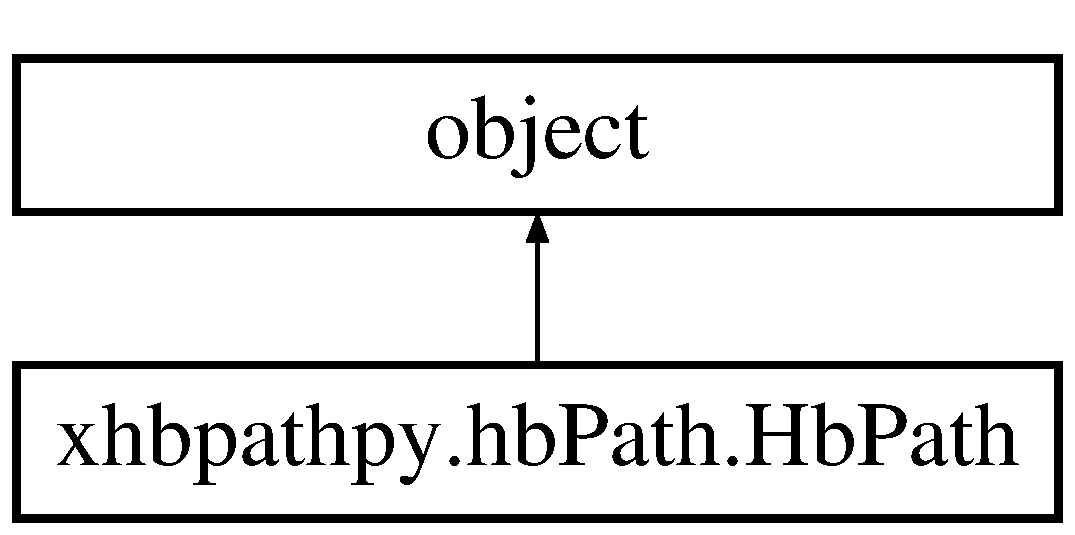
\includegraphics[height=2.000000cm]{classxhbpathpy_1_1hb_path_1_1_hb_path}
\end{center}
\end{figure}
\subsection*{Public Member Functions}
\begin{DoxyCompactItemize}
\item 
def \hyperlink{classxhbpathpy_1_1hb_path_1_1_hb_path_a5cb2ae7828572deb15b94fdd9b084905}{\-\_\-\-\_\-init\-\_\-\-\_\-}
\item 
def \hyperlink{classxhbpathpy_1_1hb_path_1_1_hb_path_a38b970ba1a1d898b8e6893051b2fb931}{load\-Path\-Info}
\begin{DoxyCompactList}\small\item\em Load the info of the pathway for a file. \end{DoxyCompactList}\item 
def \hyperlink{classxhbpathpy_1_1hb_path_1_1_hb_path_a377bdea72f8fd3afd312667ede3e08b7}{get\-All\-Hop\-Sequences}
\begin{DoxyCompactList}\small\item\em Get all the possible hopping sequences. \end{DoxyCompactList}\item 
def \hyperlink{classxhbpathpy_1_1hb_path_1_1_hb_path_a92309ee5841a1298ab5934960bcbfd26}{write\-Intermediates}
\begin{DoxyCompactList}\small\item\em Write all the intermediate states in file fname in current directory. \end{DoxyCompactList}\item 
def \hyperlink{classxhbpathpy_1_1hb_path_1_1_hb_path_a761450c9502cb09f759990bffbea1689}{write\-Hop\-Sequences}
\begin{DoxyCompactList}\small\item\em Write all the hop sequences in file fname in current directory. \end{DoxyCompactList}\item 
def \hyperlink{classxhbpathpy_1_1hb_path_1_1_hb_path_adb6647f256fb5560cfbfd58355724f04}{write\-Lowest\-Hop\-Seq}
\begin{DoxyCompactList}\small\item\em Write the lowest energy barrier hopping sequences to the file \char`\"{}fname\char`\"{}. \end{DoxyCompactList}\item 
def \hyperlink{classxhbpathpy_1_1hb_path_1_1_hb_path_a293190b627cd945f34c4564e586414ea}{evaluate\-Hop\-Seq\-Ebarrier}
\begin{DoxyCompactList}\small\item\em Calculate the energy barriers of all the hopping sequences of this pathway. \end{DoxyCompactList}\item 
def \hyperlink{classxhbpathpy_1_1hb_path_1_1_hb_path_a0b4b8d9d382c3b83d5c8d6c0b4078604}{sort\-Hop\-Seq\-By\-Ebarrier}
\begin{DoxyCompactList}\small\item\em Sort the hop sequences in the list by their energy barrier. \end{DoxyCompactList}\item 
def \hyperlink{classxhbpathpy_1_1hb_path_1_1_hb_path_aca89881c314dad892de2ce8867fda4cf}{read\-Intermediates}
\begin{DoxyCompactList}\small\item\em Load the protonation states from the file which has all the states. \end{DoxyCompactList}\item 
def \hyperlink{classxhbpathpy_1_1hb_path_1_1_hb_path_a05f97f58d06c7ed452eb57ccd4723c69}{read\-Hop\-Seqences}
\begin{DoxyCompactList}\small\item\em Load all the hopping sequences from file. \end{DoxyCompactList}\end{DoxyCompactItemize}
\subsection*{Public Attributes}
\begin{DoxyCompactItemize}
\item 
\hyperlink{classxhbpathpy_1_1hb_path_1_1_hb_path_aafe90d4a4166ba875aab2cee3012cd69}{key\-Residues}
\begin{DoxyCompactList}\small\item\em all the key residues in the pathway. \end{DoxyCompactList}\item 
\hyperlink{classxhbpathpy_1_1hb_path_1_1_hb_path_a702f32f452e98cca922244b5d003861a}{initial\-State}
\begin{DoxyCompactList}\small\item\em initial protonation state. \end{DoxyCompactList}\item 
\hyperlink{classxhbpathpy_1_1hb_path_1_1_hb_path_a35382dbb6cd72418f95343650fde976e}{hop\-Sequences}
\begin{DoxyCompactList}\small\item\em all the possible hopping sequences. \end{DoxyCompactList}\item 
\hyperlink{classxhbpathpy_1_1hb_path_1_1_hb_path_aac00fb2999e064916005328fd4032763}{protonation\-States}
\begin{DoxyCompactList}\small\item\em all the possible protonation states. \end{DoxyCompactList}\item 
\hyperlink{classxhbpathpy_1_1hb_path_1_1_hb_path_a46d9c978e67884c56826acc632b2b242}{lowest\-Energy\-Barrier}
\begin{DoxyCompactList}\small\item\em the lowest energy barrier of this pathway. \end{DoxyCompactList}\end{DoxyCompactItemize}
\subsection*{Static Public Attributes}
\begin{DoxyCompactItemize}
\item 
string \hyperlink{classxhbpathpy_1_1hb_path_1_1_hb_path_aad2661f44ffc401393a1e8f017ffdb61}{P\-A\-T\-H\-\_\-\-I\-N\-F\-O\-\_\-\-F\-I\-L\-E} = \char`\"{}pathinfo.\-txt\char`\"{}
\item 
string \hyperlink{classxhbpathpy_1_1hb_path_1_1_hb_path_a8749ebe7a54023db9c707cb93f3dbdad}{I\-N\-T\-E\-R\-M\-E\-D\-I\-A\-T\-E\-S\-\_\-\-F\-N\-A\-M\-E} = \char`\"{}intermediates.\-txt\char`\"{}
\begin{DoxyCompactList}\small\item\em file name to write all the intermediate protonation states. \end{DoxyCompactList}\item 
string \hyperlink{classxhbpathpy_1_1hb_path_1_1_hb_path_ad5130eb759eb2871a8b08e21e273c393}{H\-O\-P\-S\-E\-Q\-U\-E\-N\-C\-E\-S\-\_\-\-F\-N\-A\-M\-E} = \char`\"{}hop\-Sequences.\-txt\char`\"{}
\begin{DoxyCompactList}\small\item\em file name to write all the hopping sequences. \end{DoxyCompactList}\item 
string \hyperlink{classxhbpathpy_1_1hb_path_1_1_hb_path_a12f7c28f6247436f324bb976632b39b0}{L\-O\-W\-E\-S\-T\-H\-O\-P\-S\-E\-Q\-\_\-\-F\-N\-A\-M\-E} = \char`\"{}lowest\-Hop\-Seq.\-txt\char`\"{}
\begin{DoxyCompactList}\small\item\em file name to write the lowest energy barrier hopping sequences. \end{DoxyCompactList}\end{DoxyCompactItemize}


\subsection{Constructor \& Destructor Documentation}
\hypertarget{classxhbpathpy_1_1hb_path_1_1_hb_path_a5cb2ae7828572deb15b94fdd9b084905}{\index{xhbpathpy\-::hb\-Path\-::\-Hb\-Path@{xhbpathpy\-::hb\-Path\-::\-Hb\-Path}!\-\_\-\-\_\-init\-\_\-\-\_\-@{\-\_\-\-\_\-init\-\_\-\-\_\-}}
\index{\-\_\-\-\_\-init\-\_\-\-\_\-@{\-\_\-\-\_\-init\-\_\-\-\_\-}!xhbpathpy::hbPath::HbPath@{xhbpathpy\-::hb\-Path\-::\-Hb\-Path}}
\subsubsection[{\-\_\-\-\_\-init\-\_\-\-\_\-}]{\setlength{\rightskip}{0pt plus 5cm}def xhbpathpy.\-hb\-Path.\-Hb\-Path.\-\_\-\-\_\-init\-\_\-\-\_\- (
\begin{DoxyParamCaption}
\item[{}]{self}
\end{DoxyParamCaption}
)}}\label{classxhbpathpy_1_1hb_path_1_1_hb_path_a5cb2ae7828572deb15b94fdd9b084905}


\subsection{Member Function Documentation}
\hypertarget{classxhbpathpy_1_1hb_path_1_1_hb_path_a293190b627cd945f34c4564e586414ea}{\index{xhbpathpy\-::hb\-Path\-::\-Hb\-Path@{xhbpathpy\-::hb\-Path\-::\-Hb\-Path}!evaluate\-Hop\-Seq\-Ebarrier@{evaluate\-Hop\-Seq\-Ebarrier}}
\index{evaluate\-Hop\-Seq\-Ebarrier@{evaluate\-Hop\-Seq\-Ebarrier}!xhbpathpy::hbPath::HbPath@{xhbpathpy\-::hb\-Path\-::\-Hb\-Path}}
\subsubsection[{evaluate\-Hop\-Seq\-Ebarrier}]{\setlength{\rightskip}{0pt plus 5cm}def xhbpathpy.\-hb\-Path.\-Hb\-Path.\-evaluate\-Hop\-Seq\-Ebarrier (
\begin{DoxyParamCaption}
\item[{}]{self}
\end{DoxyParamCaption}
)}}\label{classxhbpathpy_1_1hb_path_1_1_hb_path_a293190b627cd945f34c4564e586414ea}


Calculate the energy barriers of all the hopping sequences of this pathway. 

\begin{DoxyNote}{Note}
\-: The lowest energy barrier is calculated here as well. 
\end{DoxyNote}
\hypertarget{classxhbpathpy_1_1hb_path_1_1_hb_path_a377bdea72f8fd3afd312667ede3e08b7}{\index{xhbpathpy\-::hb\-Path\-::\-Hb\-Path@{xhbpathpy\-::hb\-Path\-::\-Hb\-Path}!get\-All\-Hop\-Sequences@{get\-All\-Hop\-Sequences}}
\index{get\-All\-Hop\-Sequences@{get\-All\-Hop\-Sequences}!xhbpathpy::hbPath::HbPath@{xhbpathpy\-::hb\-Path\-::\-Hb\-Path}}
\subsubsection[{get\-All\-Hop\-Sequences}]{\setlength{\rightskip}{0pt plus 5cm}def xhbpathpy.\-hb\-Path.\-Hb\-Path.\-get\-All\-Hop\-Sequences (
\begin{DoxyParamCaption}
\item[{}]{self}
\end{DoxyParamCaption}
)}}\label{classxhbpathpy_1_1hb_path_1_1_hb_path_a377bdea72f8fd3afd312667ede3e08b7}


Get all the possible hopping sequences. 

The path has to have already loaded an initial state, and will start from the initial state. \hypertarget{classxhbpathpy_1_1hb_path_1_1_hb_path_a38b970ba1a1d898b8e6893051b2fb931}{\index{xhbpathpy\-::hb\-Path\-::\-Hb\-Path@{xhbpathpy\-::hb\-Path\-::\-Hb\-Path}!load\-Path\-Info@{load\-Path\-Info}}
\index{load\-Path\-Info@{load\-Path\-Info}!xhbpathpy::hbPath::HbPath@{xhbpathpy\-::hb\-Path\-::\-Hb\-Path}}
\subsubsection[{load\-Path\-Info}]{\setlength{\rightskip}{0pt plus 5cm}def xhbpathpy.\-hb\-Path.\-Hb\-Path.\-load\-Path\-Info (
\begin{DoxyParamCaption}
\item[{}]{self, }
\item[{}]{f\-Name = {\ttfamily {\bf P\-A\-T\-H\-\_\-\-I\-N\-F\-O\-\_\-\-F\-I\-L\-E}}}
\end{DoxyParamCaption}
)}}\label{classxhbpathpy_1_1hb_path_1_1_hb_path_a38b970ba1a1d898b8e6893051b2fb931}


Load the info of the pathway for a file. 

Get the key residues in the pathway, and their possible protonation states, and the initial state. Return an object of class Path\-Config containing this information.

The file format should be like this\-: A\-S\-P\-A0085 -\/1 0 H\-O\-H\-A0402 -\/1 0 1 H\-O\-H\-A0406 -\/1 0 1 A\-R\-G\-A0082 0 1 H\-O\-H\-A0403 -\/1 0 1 G\-L\-U\-A0194 -\/1 0 0 0 0 1 0 -\/1

The last line is the initial state. The other lines give the name of the residues, followed by all their possible protonation states. \hypertarget{classxhbpathpy_1_1hb_path_1_1_hb_path_a05f97f58d06c7ed452eb57ccd4723c69}{\index{xhbpathpy\-::hb\-Path\-::\-Hb\-Path@{xhbpathpy\-::hb\-Path\-::\-Hb\-Path}!read\-Hop\-Seqences@{read\-Hop\-Seqences}}
\index{read\-Hop\-Seqences@{read\-Hop\-Seqences}!xhbpathpy::hbPath::HbPath@{xhbpathpy\-::hb\-Path\-::\-Hb\-Path}}
\subsubsection[{read\-Hop\-Seqences}]{\setlength{\rightskip}{0pt plus 5cm}def xhbpathpy.\-hb\-Path.\-Hb\-Path.\-read\-Hop\-Seqences (
\begin{DoxyParamCaption}
\item[{}]{self, }
\item[{}]{fname = {\ttfamily {\bf H\-O\-P\-S\-E\-Q\-U\-E\-N\-C\-E\-S\-\_\-\-F\-N\-A\-M\-E}}}
\end{DoxyParamCaption}
)}}\label{classxhbpathpy_1_1hb_path_1_1_hb_path_a05f97f58d06c7ed452eb57ccd4723c69}


Load all the hopping sequences from file. 

\begin{DoxyNote}{Note}
\-: The intermediate states have to be already loaded into the pathway. 
\end{DoxyNote}
\hypertarget{classxhbpathpy_1_1hb_path_1_1_hb_path_aca89881c314dad892de2ce8867fda4cf}{\index{xhbpathpy\-::hb\-Path\-::\-Hb\-Path@{xhbpathpy\-::hb\-Path\-::\-Hb\-Path}!read\-Intermediates@{read\-Intermediates}}
\index{read\-Intermediates@{read\-Intermediates}!xhbpathpy::hbPath::HbPath@{xhbpathpy\-::hb\-Path\-::\-Hb\-Path}}
\subsubsection[{read\-Intermediates}]{\setlength{\rightskip}{0pt plus 5cm}def xhbpathpy.\-hb\-Path.\-Hb\-Path.\-read\-Intermediates (
\begin{DoxyParamCaption}
\item[{}]{self, }
\item[{}]{fname = {\ttfamily {\bf I\-N\-T\-E\-R\-M\-E\-D\-I\-A\-T\-E\-S\-\_\-\-F\-N\-A\-M\-E}}}
\end{DoxyParamCaption}
)}}\label{classxhbpathpy_1_1hb_path_1_1_hb_path_aca89881c314dad892de2ce8867fda4cf}


Load the protonation states from the file which has all the states. 

There has to be no residue already loaded into the pathway. \hypertarget{classxhbpathpy_1_1hb_path_1_1_hb_path_a0b4b8d9d382c3b83d5c8d6c0b4078604}{\index{xhbpathpy\-::hb\-Path\-::\-Hb\-Path@{xhbpathpy\-::hb\-Path\-::\-Hb\-Path}!sort\-Hop\-Seq\-By\-Ebarrier@{sort\-Hop\-Seq\-By\-Ebarrier}}
\index{sort\-Hop\-Seq\-By\-Ebarrier@{sort\-Hop\-Seq\-By\-Ebarrier}!xhbpathpy::hbPath::HbPath@{xhbpathpy\-::hb\-Path\-::\-Hb\-Path}}
\subsubsection[{sort\-Hop\-Seq\-By\-Ebarrier}]{\setlength{\rightskip}{0pt plus 5cm}def xhbpathpy.\-hb\-Path.\-Hb\-Path.\-sort\-Hop\-Seq\-By\-Ebarrier (
\begin{DoxyParamCaption}
\item[{}]{self}
\end{DoxyParamCaption}
)}}\label{classxhbpathpy_1_1hb_path_1_1_hb_path_a0b4b8d9d382c3b83d5c8d6c0b4078604}


Sort the hop sequences in the list by their energy barrier. 

\hypertarget{classxhbpathpy_1_1hb_path_1_1_hb_path_a761450c9502cb09f759990bffbea1689}{\index{xhbpathpy\-::hb\-Path\-::\-Hb\-Path@{xhbpathpy\-::hb\-Path\-::\-Hb\-Path}!write\-Hop\-Sequences@{write\-Hop\-Sequences}}
\index{write\-Hop\-Sequences@{write\-Hop\-Sequences}!xhbpathpy::hbPath::HbPath@{xhbpathpy\-::hb\-Path\-::\-Hb\-Path}}
\subsubsection[{write\-Hop\-Sequences}]{\setlength{\rightskip}{0pt plus 5cm}def xhbpathpy.\-hb\-Path.\-Hb\-Path.\-write\-Hop\-Sequences (
\begin{DoxyParamCaption}
\item[{}]{self, }
\item[{}]{fname = {\ttfamily {\bf H\-O\-P\-S\-E\-Q\-U\-E\-N\-C\-E\-S\-\_\-\-F\-N\-A\-M\-E}}}
\end{DoxyParamCaption}
)}}\label{classxhbpathpy_1_1hb_path_1_1_hb_path_a761450c9502cb09f759990bffbea1689}


Write all the hop sequences in file fname in current directory. 

\hypertarget{classxhbpathpy_1_1hb_path_1_1_hb_path_a92309ee5841a1298ab5934960bcbfd26}{\index{xhbpathpy\-::hb\-Path\-::\-Hb\-Path@{xhbpathpy\-::hb\-Path\-::\-Hb\-Path}!write\-Intermediates@{write\-Intermediates}}
\index{write\-Intermediates@{write\-Intermediates}!xhbpathpy::hbPath::HbPath@{xhbpathpy\-::hb\-Path\-::\-Hb\-Path}}
\subsubsection[{write\-Intermediates}]{\setlength{\rightskip}{0pt plus 5cm}def xhbpathpy.\-hb\-Path.\-Hb\-Path.\-write\-Intermediates (
\begin{DoxyParamCaption}
\item[{}]{self, }
\item[{}]{fname = {\ttfamily {\bf I\-N\-T\-E\-R\-M\-E\-D\-I\-A\-T\-E\-S\-\_\-\-F\-N\-A\-M\-E}}}
\end{DoxyParamCaption}
)}}\label{classxhbpathpy_1_1hb_path_1_1_hb_path_a92309ee5841a1298ab5934960bcbfd26}


Write all the intermediate states in file fname in current directory. 

\hypertarget{classxhbpathpy_1_1hb_path_1_1_hb_path_adb6647f256fb5560cfbfd58355724f04}{\index{xhbpathpy\-::hb\-Path\-::\-Hb\-Path@{xhbpathpy\-::hb\-Path\-::\-Hb\-Path}!write\-Lowest\-Hop\-Seq@{write\-Lowest\-Hop\-Seq}}
\index{write\-Lowest\-Hop\-Seq@{write\-Lowest\-Hop\-Seq}!xhbpathpy::hbPath::HbPath@{xhbpathpy\-::hb\-Path\-::\-Hb\-Path}}
\subsubsection[{write\-Lowest\-Hop\-Seq}]{\setlength{\rightskip}{0pt plus 5cm}def xhbpathpy.\-hb\-Path.\-Hb\-Path.\-write\-Lowest\-Hop\-Seq (
\begin{DoxyParamCaption}
\item[{}]{self, }
\item[{}]{fname = {\ttfamily {\bf L\-O\-W\-E\-S\-T\-H\-O\-P\-S\-E\-Q\-\_\-\-F\-N\-A\-M\-E}}}
\end{DoxyParamCaption}
)}}\label{classxhbpathpy_1_1hb_path_1_1_hb_path_adb6647f256fb5560cfbfd58355724f04}


Write the lowest energy barrier hopping sequences to the file \char`\"{}fname\char`\"{}. 

Now it's preferred to get this infor the all the hopping sequences. 

\subsection{Member Data Documentation}
\hypertarget{classxhbpathpy_1_1hb_path_1_1_hb_path_a35382dbb6cd72418f95343650fde976e}{\index{xhbpathpy\-::hb\-Path\-::\-Hb\-Path@{xhbpathpy\-::hb\-Path\-::\-Hb\-Path}!hop\-Sequences@{hop\-Sequences}}
\index{hop\-Sequences@{hop\-Sequences}!xhbpathpy::hbPath::HbPath@{xhbpathpy\-::hb\-Path\-::\-Hb\-Path}}
\subsubsection[{hop\-Sequences}]{\setlength{\rightskip}{0pt plus 5cm}xhbpathpy.\-hb\-Path.\-Hb\-Path.\-hop\-Sequences}}\label{classxhbpathpy_1_1hb_path_1_1_hb_path_a35382dbb6cd72418f95343650fde976e}


all the possible hopping sequences. 

\hypertarget{classxhbpathpy_1_1hb_path_1_1_hb_path_ad5130eb759eb2871a8b08e21e273c393}{\index{xhbpathpy\-::hb\-Path\-::\-Hb\-Path@{xhbpathpy\-::hb\-Path\-::\-Hb\-Path}!H\-O\-P\-S\-E\-Q\-U\-E\-N\-C\-E\-S\-\_\-\-F\-N\-A\-M\-E@{H\-O\-P\-S\-E\-Q\-U\-E\-N\-C\-E\-S\-\_\-\-F\-N\-A\-M\-E}}
\index{H\-O\-P\-S\-E\-Q\-U\-E\-N\-C\-E\-S\-\_\-\-F\-N\-A\-M\-E@{H\-O\-P\-S\-E\-Q\-U\-E\-N\-C\-E\-S\-\_\-\-F\-N\-A\-M\-E}!xhbpathpy::hbPath::HbPath@{xhbpathpy\-::hb\-Path\-::\-Hb\-Path}}
\subsubsection[{H\-O\-P\-S\-E\-Q\-U\-E\-N\-C\-E\-S\-\_\-\-F\-N\-A\-M\-E}]{\setlength{\rightskip}{0pt plus 5cm}string xhbpathpy.\-hb\-Path.\-Hb\-Path.\-H\-O\-P\-S\-E\-Q\-U\-E\-N\-C\-E\-S\-\_\-\-F\-N\-A\-M\-E = \char`\"{}hop\-Sequences.\-txt\char`\"{}\hspace{0.3cm}{\ttfamily [static]}}}\label{classxhbpathpy_1_1hb_path_1_1_hb_path_ad5130eb759eb2871a8b08e21e273c393}


file name to write all the hopping sequences. 

\hypertarget{classxhbpathpy_1_1hb_path_1_1_hb_path_a702f32f452e98cca922244b5d003861a}{\index{xhbpathpy\-::hb\-Path\-::\-Hb\-Path@{xhbpathpy\-::hb\-Path\-::\-Hb\-Path}!initial\-State@{initial\-State}}
\index{initial\-State@{initial\-State}!xhbpathpy::hbPath::HbPath@{xhbpathpy\-::hb\-Path\-::\-Hb\-Path}}
\subsubsection[{initial\-State}]{\setlength{\rightskip}{0pt plus 5cm}xhbpathpy.\-hb\-Path.\-Hb\-Path.\-initial\-State}}\label{classxhbpathpy_1_1hb_path_1_1_hb_path_a702f32f452e98cca922244b5d003861a}


initial protonation state. 

\hypertarget{classxhbpathpy_1_1hb_path_1_1_hb_path_a8749ebe7a54023db9c707cb93f3dbdad}{\index{xhbpathpy\-::hb\-Path\-::\-Hb\-Path@{xhbpathpy\-::hb\-Path\-::\-Hb\-Path}!I\-N\-T\-E\-R\-M\-E\-D\-I\-A\-T\-E\-S\-\_\-\-F\-N\-A\-M\-E@{I\-N\-T\-E\-R\-M\-E\-D\-I\-A\-T\-E\-S\-\_\-\-F\-N\-A\-M\-E}}
\index{I\-N\-T\-E\-R\-M\-E\-D\-I\-A\-T\-E\-S\-\_\-\-F\-N\-A\-M\-E@{I\-N\-T\-E\-R\-M\-E\-D\-I\-A\-T\-E\-S\-\_\-\-F\-N\-A\-M\-E}!xhbpathpy::hbPath::HbPath@{xhbpathpy\-::hb\-Path\-::\-Hb\-Path}}
\subsubsection[{I\-N\-T\-E\-R\-M\-E\-D\-I\-A\-T\-E\-S\-\_\-\-F\-N\-A\-M\-E}]{\setlength{\rightskip}{0pt plus 5cm}string xhbpathpy.\-hb\-Path.\-Hb\-Path.\-I\-N\-T\-E\-R\-M\-E\-D\-I\-A\-T\-E\-S\-\_\-\-F\-N\-A\-M\-E = \char`\"{}intermediates.\-txt\char`\"{}\hspace{0.3cm}{\ttfamily [static]}}}\label{classxhbpathpy_1_1hb_path_1_1_hb_path_a8749ebe7a54023db9c707cb93f3dbdad}


file name to write all the intermediate protonation states. 

\hypertarget{classxhbpathpy_1_1hb_path_1_1_hb_path_aafe90d4a4166ba875aab2cee3012cd69}{\index{xhbpathpy\-::hb\-Path\-::\-Hb\-Path@{xhbpathpy\-::hb\-Path\-::\-Hb\-Path}!key\-Residues@{key\-Residues}}
\index{key\-Residues@{key\-Residues}!xhbpathpy::hbPath::HbPath@{xhbpathpy\-::hb\-Path\-::\-Hb\-Path}}
\subsubsection[{key\-Residues}]{\setlength{\rightskip}{0pt plus 5cm}xhbpathpy.\-hb\-Path.\-Hb\-Path.\-key\-Residues}}\label{classxhbpathpy_1_1hb_path_1_1_hb_path_aafe90d4a4166ba875aab2cee3012cd69}


all the key residues in the pathway. 

\hypertarget{classxhbpathpy_1_1hb_path_1_1_hb_path_a46d9c978e67884c56826acc632b2b242}{\index{xhbpathpy\-::hb\-Path\-::\-Hb\-Path@{xhbpathpy\-::hb\-Path\-::\-Hb\-Path}!lowest\-Energy\-Barrier@{lowest\-Energy\-Barrier}}
\index{lowest\-Energy\-Barrier@{lowest\-Energy\-Barrier}!xhbpathpy::hbPath::HbPath@{xhbpathpy\-::hb\-Path\-::\-Hb\-Path}}
\subsubsection[{lowest\-Energy\-Barrier}]{\setlength{\rightskip}{0pt plus 5cm}xhbpathpy.\-hb\-Path.\-Hb\-Path.\-lowest\-Energy\-Barrier}}\label{classxhbpathpy_1_1hb_path_1_1_hb_path_a46d9c978e67884c56826acc632b2b242}


the lowest energy barrier of this pathway. 

\hypertarget{classxhbpathpy_1_1hb_path_1_1_hb_path_a12f7c28f6247436f324bb976632b39b0}{\index{xhbpathpy\-::hb\-Path\-::\-Hb\-Path@{xhbpathpy\-::hb\-Path\-::\-Hb\-Path}!L\-O\-W\-E\-S\-T\-H\-O\-P\-S\-E\-Q\-\_\-\-F\-N\-A\-M\-E@{L\-O\-W\-E\-S\-T\-H\-O\-P\-S\-E\-Q\-\_\-\-F\-N\-A\-M\-E}}
\index{L\-O\-W\-E\-S\-T\-H\-O\-P\-S\-E\-Q\-\_\-\-F\-N\-A\-M\-E@{L\-O\-W\-E\-S\-T\-H\-O\-P\-S\-E\-Q\-\_\-\-F\-N\-A\-M\-E}!xhbpathpy::hbPath::HbPath@{xhbpathpy\-::hb\-Path\-::\-Hb\-Path}}
\subsubsection[{L\-O\-W\-E\-S\-T\-H\-O\-P\-S\-E\-Q\-\_\-\-F\-N\-A\-M\-E}]{\setlength{\rightskip}{0pt plus 5cm}string xhbpathpy.\-hb\-Path.\-Hb\-Path.\-L\-O\-W\-E\-S\-T\-H\-O\-P\-S\-E\-Q\-\_\-\-F\-N\-A\-M\-E = \char`\"{}lowest\-Hop\-Seq.\-txt\char`\"{}\hspace{0.3cm}{\ttfamily [static]}}}\label{classxhbpathpy_1_1hb_path_1_1_hb_path_a12f7c28f6247436f324bb976632b39b0}


file name to write the lowest energy barrier hopping sequences. 

\hypertarget{classxhbpathpy_1_1hb_path_1_1_hb_path_aad2661f44ffc401393a1e8f017ffdb61}{\index{xhbpathpy\-::hb\-Path\-::\-Hb\-Path@{xhbpathpy\-::hb\-Path\-::\-Hb\-Path}!P\-A\-T\-H\-\_\-\-I\-N\-F\-O\-\_\-\-F\-I\-L\-E@{P\-A\-T\-H\-\_\-\-I\-N\-F\-O\-\_\-\-F\-I\-L\-E}}
\index{P\-A\-T\-H\-\_\-\-I\-N\-F\-O\-\_\-\-F\-I\-L\-E@{P\-A\-T\-H\-\_\-\-I\-N\-F\-O\-\_\-\-F\-I\-L\-E}!xhbpathpy::hbPath::HbPath@{xhbpathpy\-::hb\-Path\-::\-Hb\-Path}}
\subsubsection[{P\-A\-T\-H\-\_\-\-I\-N\-F\-O\-\_\-\-F\-I\-L\-E}]{\setlength{\rightskip}{0pt plus 5cm}string xhbpathpy.\-hb\-Path.\-Hb\-Path.\-P\-A\-T\-H\-\_\-\-I\-N\-F\-O\-\_\-\-F\-I\-L\-E = \char`\"{}pathinfo.\-txt\char`\"{}\hspace{0.3cm}{\ttfamily [static]}}}\label{classxhbpathpy_1_1hb_path_1_1_hb_path_aad2661f44ffc401393a1e8f017ffdb61}
\hypertarget{classxhbpathpy_1_1hb_path_1_1_hb_path_aac00fb2999e064916005328fd4032763}{\index{xhbpathpy\-::hb\-Path\-::\-Hb\-Path@{xhbpathpy\-::hb\-Path\-::\-Hb\-Path}!protonation\-States@{protonation\-States}}
\index{protonation\-States@{protonation\-States}!xhbpathpy::hbPath::HbPath@{xhbpathpy\-::hb\-Path\-::\-Hb\-Path}}
\subsubsection[{protonation\-States}]{\setlength{\rightskip}{0pt plus 5cm}xhbpathpy.\-hb\-Path.\-Hb\-Path.\-protonation\-States}}\label{classxhbpathpy_1_1hb_path_1_1_hb_path_aac00fb2999e064916005328fd4032763}


all the possible protonation states. 



The documentation for this class was generated from the following file\-:\begin{DoxyCompactItemize}
\item 
src/xhbpathpy/\hyperlink{hb_path_8py}{hb\-Path.\-py}\end{DoxyCompactItemize}

\hypertarget{classxhbpathpy_1_1hop_sequence_1_1_hop_sequence}{\section{xhbpathpy.\-hop\-Sequence.\-Hop\-Sequence Class Reference}
\label{classxhbpathpy_1_1hop_sequence_1_1_hop_sequence}\index{xhbpathpy.\-hop\-Sequence.\-Hop\-Sequence@{xhbpathpy.\-hop\-Sequence.\-Hop\-Sequence}}
}


Created on May 17, 2014.  


Inheritance diagram for xhbpathpy.\-hop\-Sequence.\-Hop\-Sequence\-:\begin{figure}[H]
\begin{center}
\leavevmode
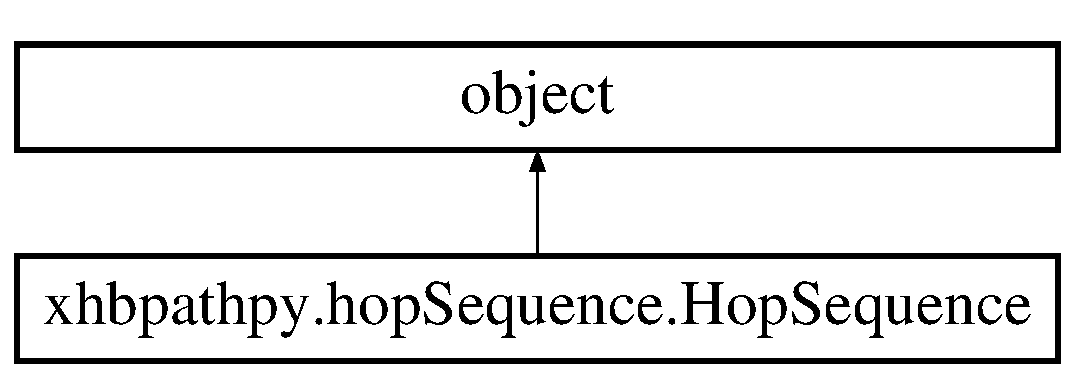
\includegraphics[height=2.000000cm]{classxhbpathpy_1_1hop_sequence_1_1_hop_sequence}
\end{center}
\end{figure}
\subsection*{Public Member Functions}
\begin{DoxyCompactItemize}
\item 
def \hyperlink{classxhbpathpy_1_1hop_sequence_1_1_hop_sequence_adc84862973bac63a8e5f500898de55c3}{\-\_\-\-\_\-init\-\_\-\-\_\-}
\item 
def \hyperlink{classxhbpathpy_1_1hop_sequence_1_1_hop_sequence_ad8e8fd6c422af62fa439fd4a9400acc4}{next\-Hop}
\begin{DoxyCompactList}\small\item\em Get all the hopping sequences from the current one by one proton hop. \end{DoxyCompactList}\item 
def \hyperlink{classxhbpathpy_1_1hop_sequence_1_1_hop_sequence_ad564ff72590f7a78c7ffc3a812dbf938}{get\-E\-Barrier}
\begin{DoxyCompactList}\small\item\em Get the energy barrier of this hop sequence. \end{DoxyCompactList}\end{DoxyCompactItemize}
\subsection*{Public Attributes}
\begin{DoxyCompactItemize}
\item 
\hyperlink{classxhbpathpy_1_1hop_sequence_1_1_hop_sequence_ae1ae68a0b84510f0eda0b61b7c533538}{possible\-Protonations}
\item 
\hyperlink{classxhbpathpy_1_1hop_sequence_1_1_hop_sequence_a5b261819492711ec0ef1e15f433ba400}{hop\-History}
\begin{DoxyCompactList}\small\item\em Save the number of times the protonation state of the residue has been changed. \end{DoxyCompactList}\item 
\hyperlink{classxhbpathpy_1_1hop_sequence_1_1_hop_sequence_af3998fce6d2d3ee13d7767730c7f9991}{energy\-Barrier}
\item 
\hyperlink{classxhbpathpy_1_1hop_sequence_1_1_hop_sequence_a45461fb5db5f5b061b07a75ebab4fa57}{intermediates}
\begin{DoxyCompactList}\small\item\em intermediate states during this hopping sequence. \end{DoxyCompactList}\end{DoxyCompactItemize}


\subsection{Detailed Description}
Created on May 17, 2014. 

\begin{DoxyAuthor}{Author}
\-: xzhu 
\end{DoxyAuthor}


\subsection{Constructor \& Destructor Documentation}
\hypertarget{classxhbpathpy_1_1hop_sequence_1_1_hop_sequence_adc84862973bac63a8e5f500898de55c3}{\index{xhbpathpy\-::hop\-Sequence\-::\-Hop\-Sequence@{xhbpathpy\-::hop\-Sequence\-::\-Hop\-Sequence}!\-\_\-\-\_\-init\-\_\-\-\_\-@{\-\_\-\-\_\-init\-\_\-\-\_\-}}
\index{\-\_\-\-\_\-init\-\_\-\-\_\-@{\-\_\-\-\_\-init\-\_\-\-\_\-}!xhbpathpy::hopSequence::HopSequence@{xhbpathpy\-::hop\-Sequence\-::\-Hop\-Sequence}}
\subsubsection[{\-\_\-\-\_\-init\-\_\-\-\_\-}]{\setlength{\rightskip}{0pt plus 5cm}def xhbpathpy.\-hop\-Sequence.\-Hop\-Sequence.\-\_\-\-\_\-init\-\_\-\-\_\- (
\begin{DoxyParamCaption}
\item[{}]{self, }
\item[{}]{initial\-State = {\ttfamily None}}
\end{DoxyParamCaption}
)}}\label{classxhbpathpy_1_1hop_sequence_1_1_hop_sequence_adc84862973bac63a8e5f500898de55c3}


\subsection{Member Function Documentation}
\hypertarget{classxhbpathpy_1_1hop_sequence_1_1_hop_sequence_ad564ff72590f7a78c7ffc3a812dbf938}{\index{xhbpathpy\-::hop\-Sequence\-::\-Hop\-Sequence@{xhbpathpy\-::hop\-Sequence\-::\-Hop\-Sequence}!get\-E\-Barrier@{get\-E\-Barrier}}
\index{get\-E\-Barrier@{get\-E\-Barrier}!xhbpathpy::hopSequence::HopSequence@{xhbpathpy\-::hop\-Sequence\-::\-Hop\-Sequence}}
\subsubsection[{get\-E\-Barrier}]{\setlength{\rightskip}{0pt plus 5cm}def xhbpathpy.\-hop\-Sequence.\-Hop\-Sequence.\-get\-E\-Barrier (
\begin{DoxyParamCaption}
\item[{}]{self}
\end{DoxyParamCaption}
)}}\label{classxhbpathpy_1_1hop_sequence_1_1_hop_sequence_ad564ff72590f7a78c7ffc3a812dbf938}


Get the energy barrier of this hop sequence. 

It's the difference between the highest energy and the energy of the initial state. The field energy\-Barrier will be reset to it. \hypertarget{classxhbpathpy_1_1hop_sequence_1_1_hop_sequence_ad8e8fd6c422af62fa439fd4a9400acc4}{\index{xhbpathpy\-::hop\-Sequence\-::\-Hop\-Sequence@{xhbpathpy\-::hop\-Sequence\-::\-Hop\-Sequence}!next\-Hop@{next\-Hop}}
\index{next\-Hop@{next\-Hop}!xhbpathpy::hopSequence::HopSequence@{xhbpathpy\-::hop\-Sequence\-::\-Hop\-Sequence}}
\subsubsection[{next\-Hop}]{\setlength{\rightskip}{0pt plus 5cm}def xhbpathpy.\-hop\-Sequence.\-Hop\-Sequence.\-next\-Hop (
\begin{DoxyParamCaption}
\item[{}]{self}
\end{DoxyParamCaption}
)}}\label{classxhbpathpy_1_1hop_sequence_1_1_hop_sequence_ad8e8fd6c422af62fa439fd4a9400acc4}


Get all the hopping sequences from the current one by one proton hop. 



\subsection{Member Data Documentation}
\hypertarget{classxhbpathpy_1_1hop_sequence_1_1_hop_sequence_af3998fce6d2d3ee13d7767730c7f9991}{\index{xhbpathpy\-::hop\-Sequence\-::\-Hop\-Sequence@{xhbpathpy\-::hop\-Sequence\-::\-Hop\-Sequence}!energy\-Barrier@{energy\-Barrier}}
\index{energy\-Barrier@{energy\-Barrier}!xhbpathpy::hopSequence::HopSequence@{xhbpathpy\-::hop\-Sequence\-::\-Hop\-Sequence}}
\subsubsection[{energy\-Barrier}]{\setlength{\rightskip}{0pt plus 5cm}xhbpathpy.\-hop\-Sequence.\-Hop\-Sequence.\-energy\-Barrier}}\label{classxhbpathpy_1_1hop_sequence_1_1_hop_sequence_af3998fce6d2d3ee13d7767730c7f9991}
\hypertarget{classxhbpathpy_1_1hop_sequence_1_1_hop_sequence_a5b261819492711ec0ef1e15f433ba400}{\index{xhbpathpy\-::hop\-Sequence\-::\-Hop\-Sequence@{xhbpathpy\-::hop\-Sequence\-::\-Hop\-Sequence}!hop\-History@{hop\-History}}
\index{hop\-History@{hop\-History}!xhbpathpy::hopSequence::HopSequence@{xhbpathpy\-::hop\-Sequence\-::\-Hop\-Sequence}}
\subsubsection[{hop\-History}]{\setlength{\rightskip}{0pt plus 5cm}xhbpathpy.\-hop\-Sequence.\-Hop\-Sequence.\-hop\-History}}\label{classxhbpathpy_1_1hop_sequence_1_1_hop_sequence_a5b261819492711ec0ef1e15f433ba400}


Save the number of times the protonation state of the residue has been changed. 

\hypertarget{classxhbpathpy_1_1hop_sequence_1_1_hop_sequence_a45461fb5db5f5b061b07a75ebab4fa57}{\index{xhbpathpy\-::hop\-Sequence\-::\-Hop\-Sequence@{xhbpathpy\-::hop\-Sequence\-::\-Hop\-Sequence}!intermediates@{intermediates}}
\index{intermediates@{intermediates}!xhbpathpy::hopSequence::HopSequence@{xhbpathpy\-::hop\-Sequence\-::\-Hop\-Sequence}}
\subsubsection[{intermediates}]{\setlength{\rightskip}{0pt plus 5cm}xhbpathpy.\-hop\-Sequence.\-Hop\-Sequence.\-intermediates}}\label{classxhbpathpy_1_1hop_sequence_1_1_hop_sequence_a45461fb5db5f5b061b07a75ebab4fa57}


intermediate states during this hopping sequence. 

\hypertarget{classxhbpathpy_1_1hop_sequence_1_1_hop_sequence_ae1ae68a0b84510f0eda0b61b7c533538}{\index{xhbpathpy\-::hop\-Sequence\-::\-Hop\-Sequence@{xhbpathpy\-::hop\-Sequence\-::\-Hop\-Sequence}!possible\-Protonations@{possible\-Protonations}}
\index{possible\-Protonations@{possible\-Protonations}!xhbpathpy::hopSequence::HopSequence@{xhbpathpy\-::hop\-Sequence\-::\-Hop\-Sequence}}
\subsubsection[{possible\-Protonations}]{\setlength{\rightskip}{0pt plus 5cm}xhbpathpy.\-hop\-Sequence.\-Hop\-Sequence.\-possible\-Protonations}}\label{classxhbpathpy_1_1hop_sequence_1_1_hop_sequence_ae1ae68a0b84510f0eda0b61b7c533538}


The documentation for this class was generated from the following file\-:\begin{DoxyCompactItemize}
\item 
src/xhbpathpy/\hyperlink{hop_sequence_8py}{hop\-Sequence.\-py}\end{DoxyCompactItemize}

\hypertarget{classhbnet_1_1_hop_sequence}{\section{hbnet.\-Hop\-Sequence Class Reference}
\label{classhbnet_1_1_hop_sequence}\index{hbnet.\-Hop\-Sequence@{hbnet.\-Hop\-Sequence}}
}
Inheritance diagram for hbnet.\-Hop\-Sequence\-:\begin{figure}[H]
\begin{center}
\leavevmode
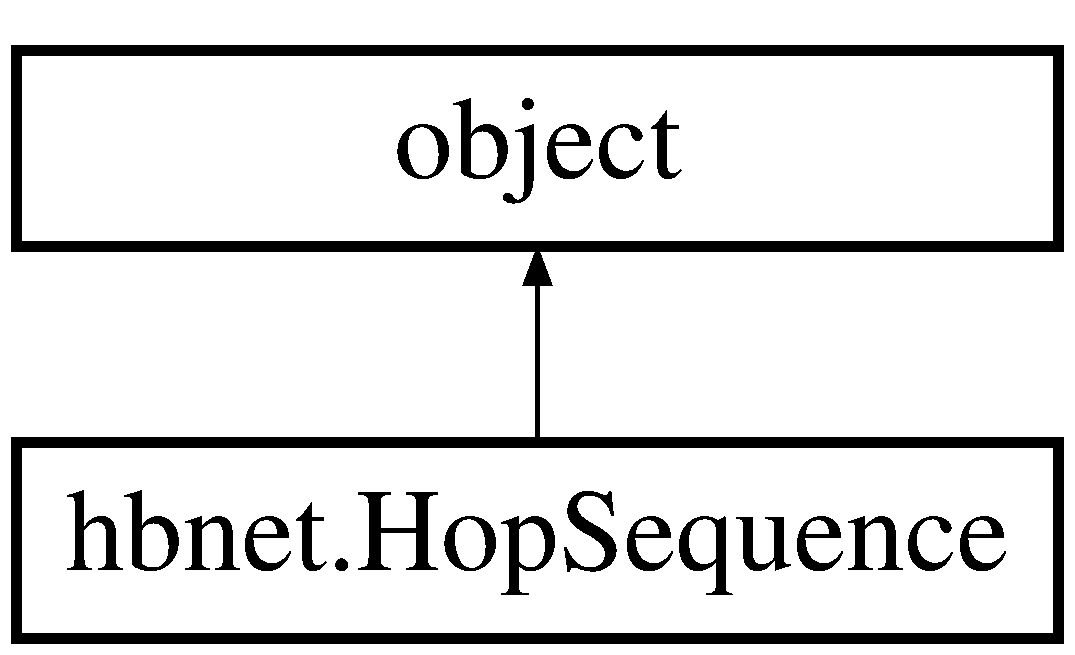
\includegraphics[height=2.000000cm]{classhbnet_1_1_hop_sequence}
\end{center}
\end{figure}
\subsection*{Public Member Functions}
\begin{DoxyCompactItemize}
\item 
def \hyperlink{classhbnet_1_1_hop_sequence_a8ce1038313142603c0040fc1e2d1e3f6}{\-\_\-\-\_\-init\-\_\-\-\_\-}
\item 
def \hyperlink{classhbnet_1_1_hop_sequence_aa5149f754e11572cd28ab071130d74c8}{next\-Hop}
\item 
def \hyperlink{classhbnet_1_1_hop_sequence_ad2d86f340617a9750077fe68c96b63f7}{get\-E\-Barrier}
\end{DoxyCompactItemize}
\subsection*{Public Attributes}
\begin{DoxyCompactItemize}
\item 
\hyperlink{classhbnet_1_1_hop_sequence_a66dd2f48420f66b8d167b4ee84d41481}{hop\-History}
\item 
\hyperlink{classhbnet_1_1_hop_sequence_a1c05eea4fe546f604fa4709ea707f07f}{energy\-Barrier}
\item 
\hyperlink{classhbnet_1_1_hop_sequence_af4dceddc7a9cf838faef6e7ea4539e58}{intermediates}
\end{DoxyCompactItemize}
\subsection*{Static Public Attributes}
\begin{DoxyCompactItemize}
\item 
list \hyperlink{classhbnet_1_1_hop_sequence_a3b83a5768107cf8e552c7f969a27374f}{possible\-Protonations} = \mbox{[}$\,$\mbox{]}
\end{DoxyCompactItemize}


\subsection{Constructor \& Destructor Documentation}
\hypertarget{classhbnet_1_1_hop_sequence_a8ce1038313142603c0040fc1e2d1e3f6}{\index{hbnet\-::\-Hop\-Sequence@{hbnet\-::\-Hop\-Sequence}!\-\_\-\-\_\-init\-\_\-\-\_\-@{\-\_\-\-\_\-init\-\_\-\-\_\-}}
\index{\-\_\-\-\_\-init\-\_\-\-\_\-@{\-\_\-\-\_\-init\-\_\-\-\_\-}!hbnet::HopSequence@{hbnet\-::\-Hop\-Sequence}}
\subsubsection[{\-\_\-\-\_\-init\-\_\-\-\_\-}]{\setlength{\rightskip}{0pt plus 5cm}def hbnet.\-Hop\-Sequence.\-\_\-\-\_\-init\-\_\-\-\_\- (
\begin{DoxyParamCaption}
\item[{}]{self, }
\item[{}]{initial\-State = {\ttfamily None}}
\end{DoxyParamCaption}
)}}\label{classhbnet_1_1_hop_sequence_a8ce1038313142603c0040fc1e2d1e3f6}


\subsection{Member Function Documentation}
\hypertarget{classhbnet_1_1_hop_sequence_ad2d86f340617a9750077fe68c96b63f7}{\index{hbnet\-::\-Hop\-Sequence@{hbnet\-::\-Hop\-Sequence}!get\-E\-Barrier@{get\-E\-Barrier}}
\index{get\-E\-Barrier@{get\-E\-Barrier}!hbnet::HopSequence@{hbnet\-::\-Hop\-Sequence}}
\subsubsection[{get\-E\-Barrier}]{\setlength{\rightskip}{0pt plus 5cm}def hbnet.\-Hop\-Sequence.\-get\-E\-Barrier (
\begin{DoxyParamCaption}
\item[{}]{self}
\end{DoxyParamCaption}
)}}\label{classhbnet_1_1_hop_sequence_ad2d86f340617a9750077fe68c96b63f7}
\hypertarget{classhbnet_1_1_hop_sequence_aa5149f754e11572cd28ab071130d74c8}{\index{hbnet\-::\-Hop\-Sequence@{hbnet\-::\-Hop\-Sequence}!next\-Hop@{next\-Hop}}
\index{next\-Hop@{next\-Hop}!hbnet::HopSequence@{hbnet\-::\-Hop\-Sequence}}
\subsubsection[{next\-Hop}]{\setlength{\rightskip}{0pt plus 5cm}def hbnet.\-Hop\-Sequence.\-next\-Hop (
\begin{DoxyParamCaption}
\item[{}]{self}
\end{DoxyParamCaption}
)}}\label{classhbnet_1_1_hop_sequence_aa5149f754e11572cd28ab071130d74c8}


\subsection{Member Data Documentation}
\hypertarget{classhbnet_1_1_hop_sequence_a1c05eea4fe546f604fa4709ea707f07f}{\index{hbnet\-::\-Hop\-Sequence@{hbnet\-::\-Hop\-Sequence}!energy\-Barrier@{energy\-Barrier}}
\index{energy\-Barrier@{energy\-Barrier}!hbnet::HopSequence@{hbnet\-::\-Hop\-Sequence}}
\subsubsection[{energy\-Barrier}]{\setlength{\rightskip}{0pt plus 5cm}hbnet.\-Hop\-Sequence.\-energy\-Barrier}}\label{classhbnet_1_1_hop_sequence_a1c05eea4fe546f604fa4709ea707f07f}
\hypertarget{classhbnet_1_1_hop_sequence_a66dd2f48420f66b8d167b4ee84d41481}{\index{hbnet\-::\-Hop\-Sequence@{hbnet\-::\-Hop\-Sequence}!hop\-History@{hop\-History}}
\index{hop\-History@{hop\-History}!hbnet::HopSequence@{hbnet\-::\-Hop\-Sequence}}
\subsubsection[{hop\-History}]{\setlength{\rightskip}{0pt plus 5cm}hbnet.\-Hop\-Sequence.\-hop\-History}}\label{classhbnet_1_1_hop_sequence_a66dd2f48420f66b8d167b4ee84d41481}
\hypertarget{classhbnet_1_1_hop_sequence_af4dceddc7a9cf838faef6e7ea4539e58}{\index{hbnet\-::\-Hop\-Sequence@{hbnet\-::\-Hop\-Sequence}!intermediates@{intermediates}}
\index{intermediates@{intermediates}!hbnet::HopSequence@{hbnet\-::\-Hop\-Sequence}}
\subsubsection[{intermediates}]{\setlength{\rightskip}{0pt plus 5cm}hbnet.\-Hop\-Sequence.\-intermediates}}\label{classhbnet_1_1_hop_sequence_af4dceddc7a9cf838faef6e7ea4539e58}
\hypertarget{classhbnet_1_1_hop_sequence_a3b83a5768107cf8e552c7f969a27374f}{\index{hbnet\-::\-Hop\-Sequence@{hbnet\-::\-Hop\-Sequence}!possible\-Protonations@{possible\-Protonations}}
\index{possible\-Protonations@{possible\-Protonations}!hbnet::HopSequence@{hbnet\-::\-Hop\-Sequence}}
\subsubsection[{possible\-Protonations}]{\setlength{\rightskip}{0pt plus 5cm}list hbnet.\-Hop\-Sequence.\-possible\-Protonations = \mbox{[}$\,$\mbox{]}\hspace{0.3cm}{\ttfamily [static]}}}\label{classhbnet_1_1_hop_sequence_a3b83a5768107cf8e552c7f969a27374f}


The documentation for this class was generated from the following file\-:\begin{DoxyCompactItemize}
\item 
src/scripts/hb\-\_\-connection/\hyperlink{hbnet_8py}{hbnet.\-py}\end{DoxyCompactItemize}

\hypertarget{classget__path__barrier_1_1_hop_sequence}{\section{get\-\_\-path\-\_\-barrier.\-Hop\-Sequence Class Reference}
\label{classget__path__barrier_1_1_hop_sequence}\index{get\-\_\-path\-\_\-barrier.\-Hop\-Sequence@{get\-\_\-path\-\_\-barrier.\-Hop\-Sequence}}
}
Inheritance diagram for get\-\_\-path\-\_\-barrier.\-Hop\-Sequence\-:\begin{figure}[H]
\begin{center}
\leavevmode
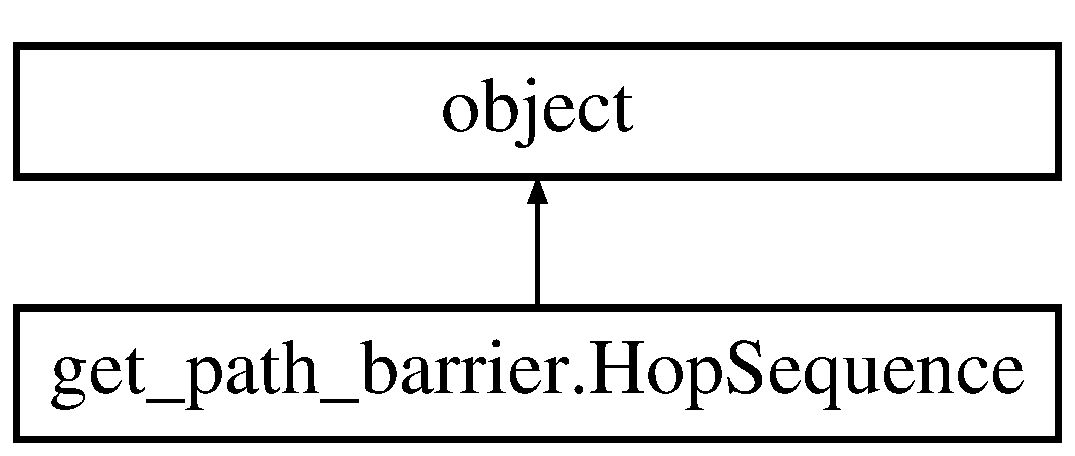
\includegraphics[height=2.000000cm]{classget__path__barrier_1_1_hop_sequence}
\end{center}
\end{figure}
\subsection*{Public Member Functions}
\begin{DoxyCompactItemize}
\item 
def \hyperlink{classget__path__barrier_1_1_hop_sequence_a3e4932d6b92f4c4cdd2c75af9139471d}{\-\_\-\-\_\-init\-\_\-\-\_\-}
\item 
def \hyperlink{classget__path__barrier_1_1_hop_sequence_ad1899d97aecd2215fd82075ce23f606a}{next\-Hop}
\item 
def \hyperlink{classget__path__barrier_1_1_hop_sequence_a50093adf1d30dca2b491fb549e3e5225}{get\-E\-Barrier}
\end{DoxyCompactItemize}
\subsection*{Public Attributes}
\begin{DoxyCompactItemize}
\item 
\hyperlink{classget__path__barrier_1_1_hop_sequence_a579cbd71947f980116542947f6fc3bb3}{hop\-History}
\item 
\hyperlink{classget__path__barrier_1_1_hop_sequence_a0bcfd627eb7a3a1adbcea611d1e4b6a6}{energy\-Barrier}
\item 
\hyperlink{classget__path__barrier_1_1_hop_sequence_aa539256b485b15e0bfb1388e832c4060}{intermediates}
\end{DoxyCompactItemize}
\subsection*{Static Public Attributes}
\begin{DoxyCompactItemize}
\item 
list \hyperlink{classget__path__barrier_1_1_hop_sequence_a1ddfff32b9b3d13841eaf9fcaceba041}{possible\-Protonations} = \mbox{[}$\,$\mbox{]}
\end{DoxyCompactItemize}


\subsection{Constructor \& Destructor Documentation}
\hypertarget{classget__path__barrier_1_1_hop_sequence_a3e4932d6b92f4c4cdd2c75af9139471d}{\index{get\-\_\-path\-\_\-barrier\-::\-Hop\-Sequence@{get\-\_\-path\-\_\-barrier\-::\-Hop\-Sequence}!\-\_\-\-\_\-init\-\_\-\-\_\-@{\-\_\-\-\_\-init\-\_\-\-\_\-}}
\index{\-\_\-\-\_\-init\-\_\-\-\_\-@{\-\_\-\-\_\-init\-\_\-\-\_\-}!get_path_barrier::HopSequence@{get\-\_\-path\-\_\-barrier\-::\-Hop\-Sequence}}
\subsubsection[{\-\_\-\-\_\-init\-\_\-\-\_\-}]{\setlength{\rightskip}{0pt plus 5cm}def get\-\_\-path\-\_\-barrier.\-Hop\-Sequence.\-\_\-\-\_\-init\-\_\-\-\_\- (
\begin{DoxyParamCaption}
\item[{}]{self, }
\item[{}]{initial\-State = {\ttfamily None}}
\end{DoxyParamCaption}
)}}\label{classget__path__barrier_1_1_hop_sequence_a3e4932d6b92f4c4cdd2c75af9139471d}


\subsection{Member Function Documentation}
\hypertarget{classget__path__barrier_1_1_hop_sequence_a50093adf1d30dca2b491fb549e3e5225}{\index{get\-\_\-path\-\_\-barrier\-::\-Hop\-Sequence@{get\-\_\-path\-\_\-barrier\-::\-Hop\-Sequence}!get\-E\-Barrier@{get\-E\-Barrier}}
\index{get\-E\-Barrier@{get\-E\-Barrier}!get_path_barrier::HopSequence@{get\-\_\-path\-\_\-barrier\-::\-Hop\-Sequence}}
\subsubsection[{get\-E\-Barrier}]{\setlength{\rightskip}{0pt plus 5cm}def get\-\_\-path\-\_\-barrier.\-Hop\-Sequence.\-get\-E\-Barrier (
\begin{DoxyParamCaption}
\item[{}]{self}
\end{DoxyParamCaption}
)}}\label{classget__path__barrier_1_1_hop_sequence_a50093adf1d30dca2b491fb549e3e5225}
\hypertarget{classget__path__barrier_1_1_hop_sequence_ad1899d97aecd2215fd82075ce23f606a}{\index{get\-\_\-path\-\_\-barrier\-::\-Hop\-Sequence@{get\-\_\-path\-\_\-barrier\-::\-Hop\-Sequence}!next\-Hop@{next\-Hop}}
\index{next\-Hop@{next\-Hop}!get_path_barrier::HopSequence@{get\-\_\-path\-\_\-barrier\-::\-Hop\-Sequence}}
\subsubsection[{next\-Hop}]{\setlength{\rightskip}{0pt plus 5cm}def get\-\_\-path\-\_\-barrier.\-Hop\-Sequence.\-next\-Hop (
\begin{DoxyParamCaption}
\item[{}]{self}
\end{DoxyParamCaption}
)}}\label{classget__path__barrier_1_1_hop_sequence_ad1899d97aecd2215fd82075ce23f606a}


\subsection{Member Data Documentation}
\hypertarget{classget__path__barrier_1_1_hop_sequence_a0bcfd627eb7a3a1adbcea611d1e4b6a6}{\index{get\-\_\-path\-\_\-barrier\-::\-Hop\-Sequence@{get\-\_\-path\-\_\-barrier\-::\-Hop\-Sequence}!energy\-Barrier@{energy\-Barrier}}
\index{energy\-Barrier@{energy\-Barrier}!get_path_barrier::HopSequence@{get\-\_\-path\-\_\-barrier\-::\-Hop\-Sequence}}
\subsubsection[{energy\-Barrier}]{\setlength{\rightskip}{0pt plus 5cm}get\-\_\-path\-\_\-barrier.\-Hop\-Sequence.\-energy\-Barrier}}\label{classget__path__barrier_1_1_hop_sequence_a0bcfd627eb7a3a1adbcea611d1e4b6a6}
\hypertarget{classget__path__barrier_1_1_hop_sequence_a579cbd71947f980116542947f6fc3bb3}{\index{get\-\_\-path\-\_\-barrier\-::\-Hop\-Sequence@{get\-\_\-path\-\_\-barrier\-::\-Hop\-Sequence}!hop\-History@{hop\-History}}
\index{hop\-History@{hop\-History}!get_path_barrier::HopSequence@{get\-\_\-path\-\_\-barrier\-::\-Hop\-Sequence}}
\subsubsection[{hop\-History}]{\setlength{\rightskip}{0pt plus 5cm}get\-\_\-path\-\_\-barrier.\-Hop\-Sequence.\-hop\-History}}\label{classget__path__barrier_1_1_hop_sequence_a579cbd71947f980116542947f6fc3bb3}
\hypertarget{classget__path__barrier_1_1_hop_sequence_aa539256b485b15e0bfb1388e832c4060}{\index{get\-\_\-path\-\_\-barrier\-::\-Hop\-Sequence@{get\-\_\-path\-\_\-barrier\-::\-Hop\-Sequence}!intermediates@{intermediates}}
\index{intermediates@{intermediates}!get_path_barrier::HopSequence@{get\-\_\-path\-\_\-barrier\-::\-Hop\-Sequence}}
\subsubsection[{intermediates}]{\setlength{\rightskip}{0pt plus 5cm}get\-\_\-path\-\_\-barrier.\-Hop\-Sequence.\-intermediates}}\label{classget__path__barrier_1_1_hop_sequence_aa539256b485b15e0bfb1388e832c4060}
\hypertarget{classget__path__barrier_1_1_hop_sequence_a1ddfff32b9b3d13841eaf9fcaceba041}{\index{get\-\_\-path\-\_\-barrier\-::\-Hop\-Sequence@{get\-\_\-path\-\_\-barrier\-::\-Hop\-Sequence}!possible\-Protonations@{possible\-Protonations}}
\index{possible\-Protonations@{possible\-Protonations}!get_path_barrier::HopSequence@{get\-\_\-path\-\_\-barrier\-::\-Hop\-Sequence}}
\subsubsection[{possible\-Protonations}]{\setlength{\rightskip}{0pt plus 5cm}list get\-\_\-path\-\_\-barrier.\-Hop\-Sequence.\-possible\-Protonations = \mbox{[}$\,$\mbox{]}\hspace{0.3cm}{\ttfamily [static]}}}\label{classget__path__barrier_1_1_hop_sequence_a1ddfff32b9b3d13841eaf9fcaceba041}


The documentation for this class was generated from the following file\-:\begin{DoxyCompactItemize}
\item 
src/path\-\_\-analysis/\hyperlink{get__path__barrier_8py}{get\-\_\-path\-\_\-barrier.\-py}\end{DoxyCompactItemize}

\hypertarget{classarg82__conn_1_1_hop_sequence}{\section{arg82\-\_\-conn.\-Hop\-Sequence Class Reference}
\label{classarg82__conn_1_1_hop_sequence}\index{arg82\-\_\-conn.\-Hop\-Sequence@{arg82\-\_\-conn.\-Hop\-Sequence}}
}
Inheritance diagram for arg82\-\_\-conn.\-Hop\-Sequence\-:\begin{figure}[H]
\begin{center}
\leavevmode
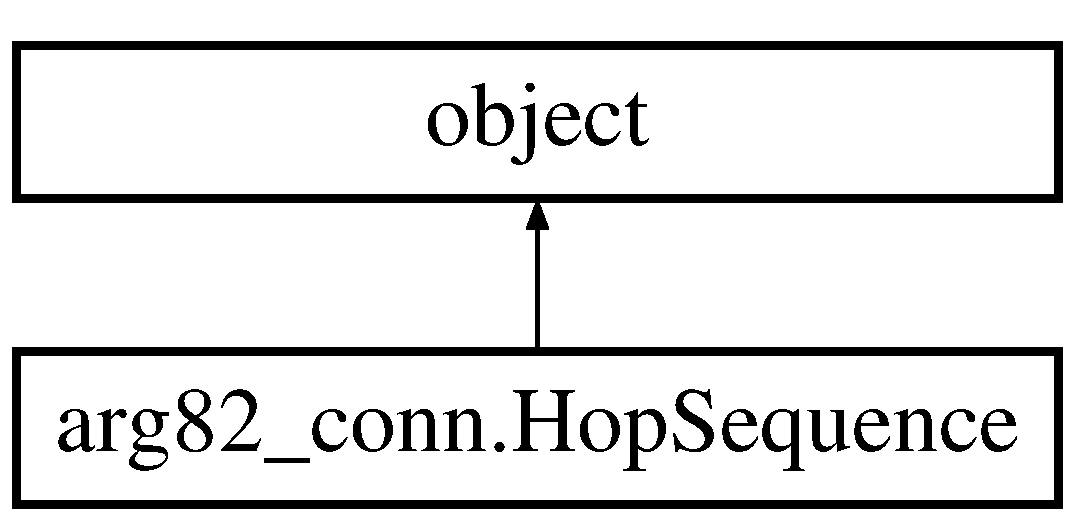
\includegraphics[height=2.000000cm]{classarg82__conn_1_1_hop_sequence}
\end{center}
\end{figure}
\subsection*{Public Member Functions}
\begin{DoxyCompactItemize}
\item 
def \hyperlink{classarg82__conn_1_1_hop_sequence_a3a1a8ee47d2b03b06d9c9fed487efa58}{\-\_\-\-\_\-init\-\_\-\-\_\-}
\item 
def \hyperlink{classarg82__conn_1_1_hop_sequence_af732d313e1d5ad598f0f8c33fba47228}{next\-Hop}
\item 
def \hyperlink{classarg82__conn_1_1_hop_sequence_a1716c182c8f86d1bb0efebbae5ccf849}{get\-E\-Barrier}
\item 
def \hyperlink{classarg82__conn_1_1_hop_sequence_a9f9bcf9ec05ac7136486ab61295be473}{print\-\_\-hop\-\_\-seqence}
\end{DoxyCompactItemize}
\subsection*{Public Attributes}
\begin{DoxyCompactItemize}
\item 
\hyperlink{classarg82__conn_1_1_hop_sequence_a149f553cca0c3ec0daa468c380abbf15}{hop\-History}
\item 
\hyperlink{classarg82__conn_1_1_hop_sequence_aae8e47b85c84f16fb9290a3bfe8f9d40}{energy\-Barrier}
\item 
\hyperlink{classarg82__conn_1_1_hop_sequence_a7012ed813fa548f9cc38ffd6ef1c8a8f}{intermediates}
\end{DoxyCompactItemize}
\subsection*{Static Public Attributes}
\begin{DoxyCompactItemize}
\item 
list \hyperlink{classarg82__conn_1_1_hop_sequence_a80cca45a252f622b1b926b641f8de7d1}{possible\-Protonations} = \mbox{[}$\,$\mbox{]}
\end{DoxyCompactItemize}


\subsection{Constructor \& Destructor Documentation}
\hypertarget{classarg82__conn_1_1_hop_sequence_a3a1a8ee47d2b03b06d9c9fed487efa58}{\index{arg82\-\_\-conn\-::\-Hop\-Sequence@{arg82\-\_\-conn\-::\-Hop\-Sequence}!\-\_\-\-\_\-init\-\_\-\-\_\-@{\-\_\-\-\_\-init\-\_\-\-\_\-}}
\index{\-\_\-\-\_\-init\-\_\-\-\_\-@{\-\_\-\-\_\-init\-\_\-\-\_\-}!arg82_conn::HopSequence@{arg82\-\_\-conn\-::\-Hop\-Sequence}}
\subsubsection[{\-\_\-\-\_\-init\-\_\-\-\_\-}]{\setlength{\rightskip}{0pt plus 5cm}def arg82\-\_\-conn.\-Hop\-Sequence.\-\_\-\-\_\-init\-\_\-\-\_\- (
\begin{DoxyParamCaption}
\item[{}]{self, }
\item[{}]{initial\-State = {\ttfamily None}}
\end{DoxyParamCaption}
)}}\label{classarg82__conn_1_1_hop_sequence_a3a1a8ee47d2b03b06d9c9fed487efa58}


\subsection{Member Function Documentation}
\hypertarget{classarg82__conn_1_1_hop_sequence_a1716c182c8f86d1bb0efebbae5ccf849}{\index{arg82\-\_\-conn\-::\-Hop\-Sequence@{arg82\-\_\-conn\-::\-Hop\-Sequence}!get\-E\-Barrier@{get\-E\-Barrier}}
\index{get\-E\-Barrier@{get\-E\-Barrier}!arg82_conn::HopSequence@{arg82\-\_\-conn\-::\-Hop\-Sequence}}
\subsubsection[{get\-E\-Barrier}]{\setlength{\rightskip}{0pt plus 5cm}def arg82\-\_\-conn.\-Hop\-Sequence.\-get\-E\-Barrier (
\begin{DoxyParamCaption}
\item[{}]{self}
\end{DoxyParamCaption}
)}}\label{classarg82__conn_1_1_hop_sequence_a1716c182c8f86d1bb0efebbae5ccf849}
\hypertarget{classarg82__conn_1_1_hop_sequence_af732d313e1d5ad598f0f8c33fba47228}{\index{arg82\-\_\-conn\-::\-Hop\-Sequence@{arg82\-\_\-conn\-::\-Hop\-Sequence}!next\-Hop@{next\-Hop}}
\index{next\-Hop@{next\-Hop}!arg82_conn::HopSequence@{arg82\-\_\-conn\-::\-Hop\-Sequence}}
\subsubsection[{next\-Hop}]{\setlength{\rightskip}{0pt plus 5cm}def arg82\-\_\-conn.\-Hop\-Sequence.\-next\-Hop (
\begin{DoxyParamCaption}
\item[{}]{self}
\end{DoxyParamCaption}
)}}\label{classarg82__conn_1_1_hop_sequence_af732d313e1d5ad598f0f8c33fba47228}
\hypertarget{classarg82__conn_1_1_hop_sequence_a9f9bcf9ec05ac7136486ab61295be473}{\index{arg82\-\_\-conn\-::\-Hop\-Sequence@{arg82\-\_\-conn\-::\-Hop\-Sequence}!print\-\_\-hop\-\_\-seqence@{print\-\_\-hop\-\_\-seqence}}
\index{print\-\_\-hop\-\_\-seqence@{print\-\_\-hop\-\_\-seqence}!arg82_conn::HopSequence@{arg82\-\_\-conn\-::\-Hop\-Sequence}}
\subsubsection[{print\-\_\-hop\-\_\-seqence}]{\setlength{\rightskip}{0pt plus 5cm}def arg82\-\_\-conn.\-Hop\-Sequence.\-print\-\_\-hop\-\_\-seqence (
\begin{DoxyParamCaption}
\item[{}]{self}
\end{DoxyParamCaption}
)}}\label{classarg82__conn_1_1_hop_sequence_a9f9bcf9ec05ac7136486ab61295be473}


\subsection{Member Data Documentation}
\hypertarget{classarg82__conn_1_1_hop_sequence_aae8e47b85c84f16fb9290a3bfe8f9d40}{\index{arg82\-\_\-conn\-::\-Hop\-Sequence@{arg82\-\_\-conn\-::\-Hop\-Sequence}!energy\-Barrier@{energy\-Barrier}}
\index{energy\-Barrier@{energy\-Barrier}!arg82_conn::HopSequence@{arg82\-\_\-conn\-::\-Hop\-Sequence}}
\subsubsection[{energy\-Barrier}]{\setlength{\rightskip}{0pt plus 5cm}arg82\-\_\-conn.\-Hop\-Sequence.\-energy\-Barrier}}\label{classarg82__conn_1_1_hop_sequence_aae8e47b85c84f16fb9290a3bfe8f9d40}
\hypertarget{classarg82__conn_1_1_hop_sequence_a149f553cca0c3ec0daa468c380abbf15}{\index{arg82\-\_\-conn\-::\-Hop\-Sequence@{arg82\-\_\-conn\-::\-Hop\-Sequence}!hop\-History@{hop\-History}}
\index{hop\-History@{hop\-History}!arg82_conn::HopSequence@{arg82\-\_\-conn\-::\-Hop\-Sequence}}
\subsubsection[{hop\-History}]{\setlength{\rightskip}{0pt plus 5cm}arg82\-\_\-conn.\-Hop\-Sequence.\-hop\-History}}\label{classarg82__conn_1_1_hop_sequence_a149f553cca0c3ec0daa468c380abbf15}
\hypertarget{classarg82__conn_1_1_hop_sequence_a7012ed813fa548f9cc38ffd6ef1c8a8f}{\index{arg82\-\_\-conn\-::\-Hop\-Sequence@{arg82\-\_\-conn\-::\-Hop\-Sequence}!intermediates@{intermediates}}
\index{intermediates@{intermediates}!arg82_conn::HopSequence@{arg82\-\_\-conn\-::\-Hop\-Sequence}}
\subsubsection[{intermediates}]{\setlength{\rightskip}{0pt plus 5cm}arg82\-\_\-conn.\-Hop\-Sequence.\-intermediates}}\label{classarg82__conn_1_1_hop_sequence_a7012ed813fa548f9cc38ffd6ef1c8a8f}
\hypertarget{classarg82__conn_1_1_hop_sequence_a80cca45a252f622b1b926b641f8de7d1}{\index{arg82\-\_\-conn\-::\-Hop\-Sequence@{arg82\-\_\-conn\-::\-Hop\-Sequence}!possible\-Protonations@{possible\-Protonations}}
\index{possible\-Protonations@{possible\-Protonations}!arg82_conn::HopSequence@{arg82\-\_\-conn\-::\-Hop\-Sequence}}
\subsubsection[{possible\-Protonations}]{\setlength{\rightskip}{0pt plus 5cm}list arg82\-\_\-conn.\-Hop\-Sequence.\-possible\-Protonations = \mbox{[}$\,$\mbox{]}\hspace{0.3cm}{\ttfamily [static]}}}\label{classarg82__conn_1_1_hop_sequence_a80cca45a252f622b1b926b641f8de7d1}


The documentation for this class was generated from the following file\-:\begin{DoxyCompactItemize}
\item 
src/scripts/hb\-\_\-connection/\hyperlink{arg82__conn_8py}{arg82\-\_\-conn.\-py}\end{DoxyCompactItemize}

\hypertarget{classsetuptest_1_1_m_c_run_type}{\section{setuptest.\-M\-C\-Run\-Type Class Reference}
\label{classsetuptest_1_1_m_c_run_type}\index{setuptest.\-M\-C\-Run\-Type@{setuptest.\-M\-C\-Run\-Type}}
}
Inheritance diagram for setuptest.\-M\-C\-Run\-Type\-:\begin{figure}[H]
\begin{center}
\leavevmode
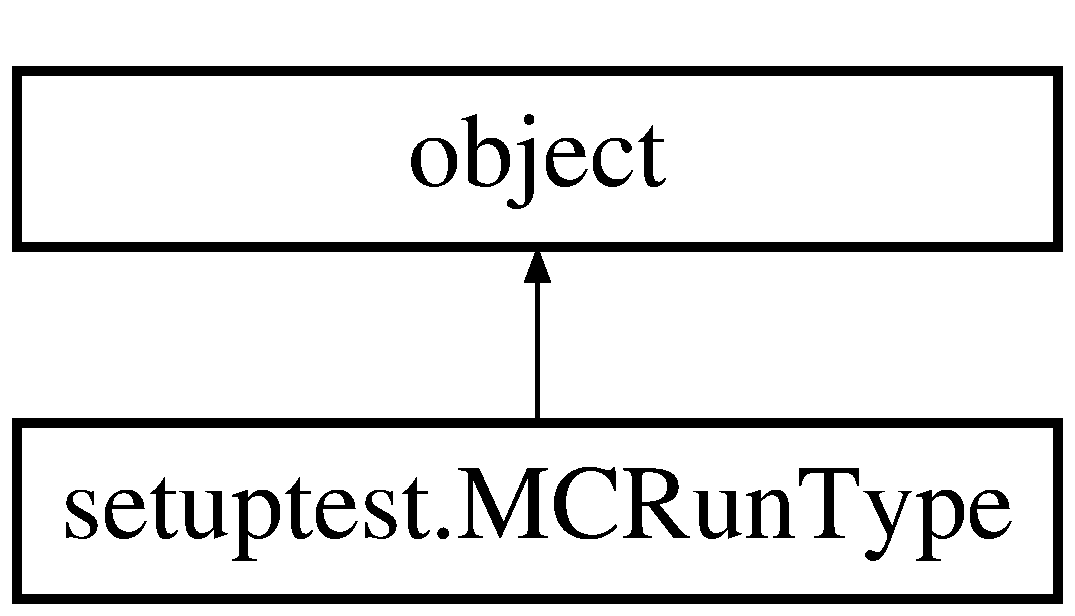
\includegraphics[height=2.000000cm]{classsetuptest_1_1_m_c_run_type}
\end{center}
\end{figure}
\subsection*{Public Member Functions}
\begin{DoxyCompactItemize}
\item 
def \hyperlink{classsetuptest_1_1_m_c_run_type_a291ead26e72bb3ded1a7248f87a554b2}{\-\_\-\-\_\-init\-\_\-\-\_\-}
\item 
def \hyperlink{classsetuptest_1_1_m_c_run_type_a4a474d1557bac832e58e9ce56f242156}{submit\-Test}
\item 
def \hyperlink{classsetuptest_1_1_m_c_run_type_a6713b47776d33b8025e6b09416f957f3}{check\-Finish\-Status}
\item 
def \hyperlink{classsetuptest_1_1_m_c_run_type_a186dd2614f1ce577d282b2ed35b0dc93}{get\-Stat}
\begin{DoxyCompactList}\small\item\em Get a statistics of the runs. \end{DoxyCompactList}\end{DoxyCompactItemize}
\subsection*{Public Attributes}
\begin{DoxyCompactItemize}
\item 
\hyperlink{classsetuptest_1_1_m_c_run_type_af5e0eb81651753179f30f5aa0b5b752d}{annealing}
\item 
\hyperlink{classsetuptest_1_1_m_c_run_type_a5272a45924d8654ce945c38c88f3dc9b}{equilibration}
\item 
\hyperlink{classsetuptest_1_1_m_c_run_type_a12080b15b53b6e84f1d1371b0c07f8e1}{sampling}
\item 
\hyperlink{classsetuptest_1_1_m_c_run_type_a3a82e9807477fde197a24b19e9f69b7b}{indep}
\item 
\hyperlink{classsetuptest_1_1_m_c_run_type_acb7e778c56d745bf4c5db094300ad82e}{run\-Id}
\item 
\hyperlink{classsetuptest_1_1_m_c_run_type_a1bad9d54294b8ef33e47ee96b19fa237}{name}
\item 
\hyperlink{classsetuptest_1_1_m_c_run_type_aa08e009de5f3dda3b5f0c54c932fefa8}{n\-Subtest}
\item 
\hyperlink{classsetuptest_1_1_m_c_run_type_a3a5551a4545b38a08767cc3074c4b525}{avg\-Energy}
\item 
\hyperlink{classsetuptest_1_1_m_c_run_type_abf6e141931490ebd048577558ca0eb87}{std\-Avg\-Energy}
\item 
\hyperlink{classsetuptest_1_1_m_c_run_type_a5862b8254f7872d0781be684d65fe6e3}{avg\-Confsg}
\end{DoxyCompactItemize}


\subsection{Constructor \& Destructor Documentation}
\hypertarget{classsetuptest_1_1_m_c_run_type_a291ead26e72bb3ded1a7248f87a554b2}{\index{setuptest\-::\-M\-C\-Run\-Type@{setuptest\-::\-M\-C\-Run\-Type}!\-\_\-\-\_\-init\-\_\-\-\_\-@{\-\_\-\-\_\-init\-\_\-\-\_\-}}
\index{\-\_\-\-\_\-init\-\_\-\-\_\-@{\-\_\-\-\_\-init\-\_\-\-\_\-}!setuptest::MCRunType@{setuptest\-::\-M\-C\-Run\-Type}}
\subsubsection[{\-\_\-\-\_\-init\-\_\-\-\_\-}]{\setlength{\rightskip}{0pt plus 5cm}def setuptest.\-M\-C\-Run\-Type.\-\_\-\-\_\-init\-\_\-\-\_\- (
\begin{DoxyParamCaption}
\item[{}]{self, }
\item[{}]{a = {\ttfamily 100}, }
\item[{}]{e = {\ttfamily 300}, }
\item[{}]{s = {\ttfamily 2000}, }
\item[{}]{i = {\ttfamily 6}}
\end{DoxyParamCaption}
)}}\label{classsetuptest_1_1_m_c_run_type_a291ead26e72bb3ded1a7248f87a554b2}


\subsection{Member Function Documentation}
\hypertarget{classsetuptest_1_1_m_c_run_type_a6713b47776d33b8025e6b09416f957f3}{\index{setuptest\-::\-M\-C\-Run\-Type@{setuptest\-::\-M\-C\-Run\-Type}!check\-Finish\-Status@{check\-Finish\-Status}}
\index{check\-Finish\-Status@{check\-Finish\-Status}!setuptest::MCRunType@{setuptest\-::\-M\-C\-Run\-Type}}
\subsubsection[{check\-Finish\-Status}]{\setlength{\rightskip}{0pt plus 5cm}def setuptest.\-M\-C\-Run\-Type.\-check\-Finish\-Status (
\begin{DoxyParamCaption}
\item[{}]{self, }
\item[{}]{work\-Path}
\end{DoxyParamCaption}
)}}\label{classsetuptest_1_1_m_c_run_type_a6713b47776d33b8025e6b09416f957f3}
\hypertarget{classsetuptest_1_1_m_c_run_type_a186dd2614f1ce577d282b2ed35b0dc93}{\index{setuptest\-::\-M\-C\-Run\-Type@{setuptest\-::\-M\-C\-Run\-Type}!get\-Stat@{get\-Stat}}
\index{get\-Stat@{get\-Stat}!setuptest::MCRunType@{setuptest\-::\-M\-C\-Run\-Type}}
\subsubsection[{get\-Stat}]{\setlength{\rightskip}{0pt plus 5cm}def setuptest.\-M\-C\-Run\-Type.\-get\-Stat (
\begin{DoxyParamCaption}
\item[{}]{self, }
\item[{}]{work\-Path}
\end{DoxyParamCaption}
)}}\label{classsetuptest_1_1_m_c_run_type_a186dd2614f1ce577d282b2ed35b0dc93}


Get a statistics of the runs. 

\hypertarget{classsetuptest_1_1_m_c_run_type_a4a474d1557bac832e58e9ce56f242156}{\index{setuptest\-::\-M\-C\-Run\-Type@{setuptest\-::\-M\-C\-Run\-Type}!submit\-Test@{submit\-Test}}
\index{submit\-Test@{submit\-Test}!setuptest::MCRunType@{setuptest\-::\-M\-C\-Run\-Type}}
\subsubsection[{submit\-Test}]{\setlength{\rightskip}{0pt plus 5cm}def setuptest.\-M\-C\-Run\-Type.\-submit\-Test (
\begin{DoxyParamCaption}
\item[{}]{self, }
\item[{}]{parent\-Path, }
\item[{}]{work\-Path}
\end{DoxyParamCaption}
)}}\label{classsetuptest_1_1_m_c_run_type_a4a474d1557bac832e58e9ce56f242156}


\subsection{Member Data Documentation}
\hypertarget{classsetuptest_1_1_m_c_run_type_af5e0eb81651753179f30f5aa0b5b752d}{\index{setuptest\-::\-M\-C\-Run\-Type@{setuptest\-::\-M\-C\-Run\-Type}!annealing@{annealing}}
\index{annealing@{annealing}!setuptest::MCRunType@{setuptest\-::\-M\-C\-Run\-Type}}
\subsubsection[{annealing}]{\setlength{\rightskip}{0pt plus 5cm}setuptest.\-M\-C\-Run\-Type.\-annealing}}\label{classsetuptest_1_1_m_c_run_type_af5e0eb81651753179f30f5aa0b5b752d}
\hypertarget{classsetuptest_1_1_m_c_run_type_a5862b8254f7872d0781be684d65fe6e3}{\index{setuptest\-::\-M\-C\-Run\-Type@{setuptest\-::\-M\-C\-Run\-Type}!avg\-Confsg@{avg\-Confsg}}
\index{avg\-Confsg@{avg\-Confsg}!setuptest::MCRunType@{setuptest\-::\-M\-C\-Run\-Type}}
\subsubsection[{avg\-Confsg}]{\setlength{\rightskip}{0pt plus 5cm}setuptest.\-M\-C\-Run\-Type.\-avg\-Confsg}}\label{classsetuptest_1_1_m_c_run_type_a5862b8254f7872d0781be684d65fe6e3}
\hypertarget{classsetuptest_1_1_m_c_run_type_a3a5551a4545b38a08767cc3074c4b525}{\index{setuptest\-::\-M\-C\-Run\-Type@{setuptest\-::\-M\-C\-Run\-Type}!avg\-Energy@{avg\-Energy}}
\index{avg\-Energy@{avg\-Energy}!setuptest::MCRunType@{setuptest\-::\-M\-C\-Run\-Type}}
\subsubsection[{avg\-Energy}]{\setlength{\rightskip}{0pt plus 5cm}setuptest.\-M\-C\-Run\-Type.\-avg\-Energy}}\label{classsetuptest_1_1_m_c_run_type_a3a5551a4545b38a08767cc3074c4b525}
\hypertarget{classsetuptest_1_1_m_c_run_type_a5272a45924d8654ce945c38c88f3dc9b}{\index{setuptest\-::\-M\-C\-Run\-Type@{setuptest\-::\-M\-C\-Run\-Type}!equilibration@{equilibration}}
\index{equilibration@{equilibration}!setuptest::MCRunType@{setuptest\-::\-M\-C\-Run\-Type}}
\subsubsection[{equilibration}]{\setlength{\rightskip}{0pt plus 5cm}setuptest.\-M\-C\-Run\-Type.\-equilibration}}\label{classsetuptest_1_1_m_c_run_type_a5272a45924d8654ce945c38c88f3dc9b}
\hypertarget{classsetuptest_1_1_m_c_run_type_a3a82e9807477fde197a24b19e9f69b7b}{\index{setuptest\-::\-M\-C\-Run\-Type@{setuptest\-::\-M\-C\-Run\-Type}!indep@{indep}}
\index{indep@{indep}!setuptest::MCRunType@{setuptest\-::\-M\-C\-Run\-Type}}
\subsubsection[{indep}]{\setlength{\rightskip}{0pt plus 5cm}setuptest.\-M\-C\-Run\-Type.\-indep}}\label{classsetuptest_1_1_m_c_run_type_a3a82e9807477fde197a24b19e9f69b7b}
\hypertarget{classsetuptest_1_1_m_c_run_type_a1bad9d54294b8ef33e47ee96b19fa237}{\index{setuptest\-::\-M\-C\-Run\-Type@{setuptest\-::\-M\-C\-Run\-Type}!name@{name}}
\index{name@{name}!setuptest::MCRunType@{setuptest\-::\-M\-C\-Run\-Type}}
\subsubsection[{name}]{\setlength{\rightskip}{0pt plus 5cm}setuptest.\-M\-C\-Run\-Type.\-name}}\label{classsetuptest_1_1_m_c_run_type_a1bad9d54294b8ef33e47ee96b19fa237}
\hypertarget{classsetuptest_1_1_m_c_run_type_aa08e009de5f3dda3b5f0c54c932fefa8}{\index{setuptest\-::\-M\-C\-Run\-Type@{setuptest\-::\-M\-C\-Run\-Type}!n\-Subtest@{n\-Subtest}}
\index{n\-Subtest@{n\-Subtest}!setuptest::MCRunType@{setuptest\-::\-M\-C\-Run\-Type}}
\subsubsection[{n\-Subtest}]{\setlength{\rightskip}{0pt plus 5cm}setuptest.\-M\-C\-Run\-Type.\-n\-Subtest}}\label{classsetuptest_1_1_m_c_run_type_aa08e009de5f3dda3b5f0c54c932fefa8}
\hypertarget{classsetuptest_1_1_m_c_run_type_acb7e778c56d745bf4c5db094300ad82e}{\index{setuptest\-::\-M\-C\-Run\-Type@{setuptest\-::\-M\-C\-Run\-Type}!run\-Id@{run\-Id}}
\index{run\-Id@{run\-Id}!setuptest::MCRunType@{setuptest\-::\-M\-C\-Run\-Type}}
\subsubsection[{run\-Id}]{\setlength{\rightskip}{0pt plus 5cm}setuptest.\-M\-C\-Run\-Type.\-run\-Id}}\label{classsetuptest_1_1_m_c_run_type_acb7e778c56d745bf4c5db094300ad82e}
\hypertarget{classsetuptest_1_1_m_c_run_type_a12080b15b53b6e84f1d1371b0c07f8e1}{\index{setuptest\-::\-M\-C\-Run\-Type@{setuptest\-::\-M\-C\-Run\-Type}!sampling@{sampling}}
\index{sampling@{sampling}!setuptest::MCRunType@{setuptest\-::\-M\-C\-Run\-Type}}
\subsubsection[{sampling}]{\setlength{\rightskip}{0pt plus 5cm}setuptest.\-M\-C\-Run\-Type.\-sampling}}\label{classsetuptest_1_1_m_c_run_type_a12080b15b53b6e84f1d1371b0c07f8e1}
\hypertarget{classsetuptest_1_1_m_c_run_type_abf6e141931490ebd048577558ca0eb87}{\index{setuptest\-::\-M\-C\-Run\-Type@{setuptest\-::\-M\-C\-Run\-Type}!std\-Avg\-Energy@{std\-Avg\-Energy}}
\index{std\-Avg\-Energy@{std\-Avg\-Energy}!setuptest::MCRunType@{setuptest\-::\-M\-C\-Run\-Type}}
\subsubsection[{std\-Avg\-Energy}]{\setlength{\rightskip}{0pt plus 5cm}setuptest.\-M\-C\-Run\-Type.\-std\-Avg\-Energy}}\label{classsetuptest_1_1_m_c_run_type_abf6e141931490ebd048577558ca0eb87}


The documentation for this class was generated from the following file\-:\begin{DoxyCompactItemize}
\item 
src/scripts/old/\hyperlink{setuptest_8py}{setuptest.\-py}\end{DoxyCompactItemize}

\hypertarget{classxmccepy_1_1mp_1_1_p_r_o_t_e_i_n}{\section{xmccepy.\-mp.\-P\-R\-O\-T\-E\-I\-N Class Reference}
\label{classxmccepy_1_1mp_1_1_p_r_o_t_e_i_n}\index{xmccepy.\-mp.\-P\-R\-O\-T\-E\-I\-N@{xmccepy.\-mp.\-P\-R\-O\-T\-E\-I\-N}}
}
\subsection*{Public Member Functions}
\begin{DoxyCompactItemize}
\item 
def \hyperlink{classxmccepy_1_1mp_1_1_p_r_o_t_e_i_n_a7e26d4d1cfd60c6a5193c141971dbc05}{\-\_\-\-\_\-init\-\_\-\-\_\-}
\item 
def \hyperlink{classxmccepy_1_1mp_1_1_p_r_o_t_e_i_n_a64b0e15c69b786fa85740bd7416b6d42}{read\-P\-D\-B}
\item 
def \hyperlink{classxmccepy_1_1mp_1_1_p_r_o_t_e_i_n_ae9f72597d99182414e3afe867d0c0997}{write\-P\-D\-B}
\end{DoxyCompactItemize}
\subsection*{Public Attributes}
\begin{DoxyCompactItemize}
\item 
\hyperlink{classxmccepy_1_1mp_1_1_p_r_o_t_e_i_n_ae97e1a5a6da630ad7de620df7ce17439}{ress}
\end{DoxyCompactItemize}


\subsection{Constructor \& Destructor Documentation}
\hypertarget{classxmccepy_1_1mp_1_1_p_r_o_t_e_i_n_a7e26d4d1cfd60c6a5193c141971dbc05}{\index{xmccepy\-::mp\-::\-P\-R\-O\-T\-E\-I\-N@{xmccepy\-::mp\-::\-P\-R\-O\-T\-E\-I\-N}!\-\_\-\-\_\-init\-\_\-\-\_\-@{\-\_\-\-\_\-init\-\_\-\-\_\-}}
\index{\-\_\-\-\_\-init\-\_\-\-\_\-@{\-\_\-\-\_\-init\-\_\-\-\_\-}!xmccepy::mp::PROTEIN@{xmccepy\-::mp\-::\-P\-R\-O\-T\-E\-I\-N}}
\subsubsection[{\-\_\-\-\_\-init\-\_\-\-\_\-}]{\setlength{\rightskip}{0pt plus 5cm}def xmccepy.\-mp.\-P\-R\-O\-T\-E\-I\-N.\-\_\-\-\_\-init\-\_\-\-\_\- (
\begin{DoxyParamCaption}
\item[{}]{self}
\end{DoxyParamCaption}
)}}\label{classxmccepy_1_1mp_1_1_p_r_o_t_e_i_n_a7e26d4d1cfd60c6a5193c141971dbc05}


\subsection{Member Function Documentation}
\hypertarget{classxmccepy_1_1mp_1_1_p_r_o_t_e_i_n_a64b0e15c69b786fa85740bd7416b6d42}{\index{xmccepy\-::mp\-::\-P\-R\-O\-T\-E\-I\-N@{xmccepy\-::mp\-::\-P\-R\-O\-T\-E\-I\-N}!read\-P\-D\-B@{read\-P\-D\-B}}
\index{read\-P\-D\-B@{read\-P\-D\-B}!xmccepy::mp::PROTEIN@{xmccepy\-::mp\-::\-P\-R\-O\-T\-E\-I\-N}}
\subsubsection[{read\-P\-D\-B}]{\setlength{\rightskip}{0pt plus 5cm}def xmccepy.\-mp.\-P\-R\-O\-T\-E\-I\-N.\-read\-P\-D\-B (
\begin{DoxyParamCaption}
\item[{}]{self, }
\item[{}]{fname}
\end{DoxyParamCaption}
)}}\label{classxmccepy_1_1mp_1_1_p_r_o_t_e_i_n_a64b0e15c69b786fa85740bd7416b6d42}
\hypertarget{classxmccepy_1_1mp_1_1_p_r_o_t_e_i_n_ae9f72597d99182414e3afe867d0c0997}{\index{xmccepy\-::mp\-::\-P\-R\-O\-T\-E\-I\-N@{xmccepy\-::mp\-::\-P\-R\-O\-T\-E\-I\-N}!write\-P\-D\-B@{write\-P\-D\-B}}
\index{write\-P\-D\-B@{write\-P\-D\-B}!xmccepy::mp::PROTEIN@{xmccepy\-::mp\-::\-P\-R\-O\-T\-E\-I\-N}}
\subsubsection[{write\-P\-D\-B}]{\setlength{\rightskip}{0pt plus 5cm}def xmccepy.\-mp.\-P\-R\-O\-T\-E\-I\-N.\-write\-P\-D\-B (
\begin{DoxyParamCaption}
\item[{}]{self}
\end{DoxyParamCaption}
)}}\label{classxmccepy_1_1mp_1_1_p_r_o_t_e_i_n_ae9f72597d99182414e3afe867d0c0997}


\subsection{Member Data Documentation}
\hypertarget{classxmccepy_1_1mp_1_1_p_r_o_t_e_i_n_ae97e1a5a6da630ad7de620df7ce17439}{\index{xmccepy\-::mp\-::\-P\-R\-O\-T\-E\-I\-N@{xmccepy\-::mp\-::\-P\-R\-O\-T\-E\-I\-N}!ress@{ress}}
\index{ress@{ress}!xmccepy::mp::PROTEIN@{xmccepy\-::mp\-::\-P\-R\-O\-T\-E\-I\-N}}
\subsubsection[{ress}]{\setlength{\rightskip}{0pt plus 5cm}xmccepy.\-mp.\-P\-R\-O\-T\-E\-I\-N.\-ress}}\label{classxmccepy_1_1mp_1_1_p_r_o_t_e_i_n_ae97e1a5a6da630ad7de620df7ce17439}


The documentation for this class was generated from the following file\-:\begin{DoxyCompactItemize}
\item 
src/xmccepy/\hyperlink{mp_8py}{mp.\-py}\end{DoxyCompactItemize}

\hypertarget{classarg82__conn_1_1_protonation_state}{\section{arg82\-\_\-conn.\-Protonation\-State Class Reference}
\label{classarg82__conn_1_1_protonation_state}\index{arg82\-\_\-conn.\-Protonation\-State@{arg82\-\_\-conn.\-Protonation\-State}}
}
Inheritance diagram for arg82\-\_\-conn.\-Protonation\-State\-:\begin{figure}[H]
\begin{center}
\leavevmode
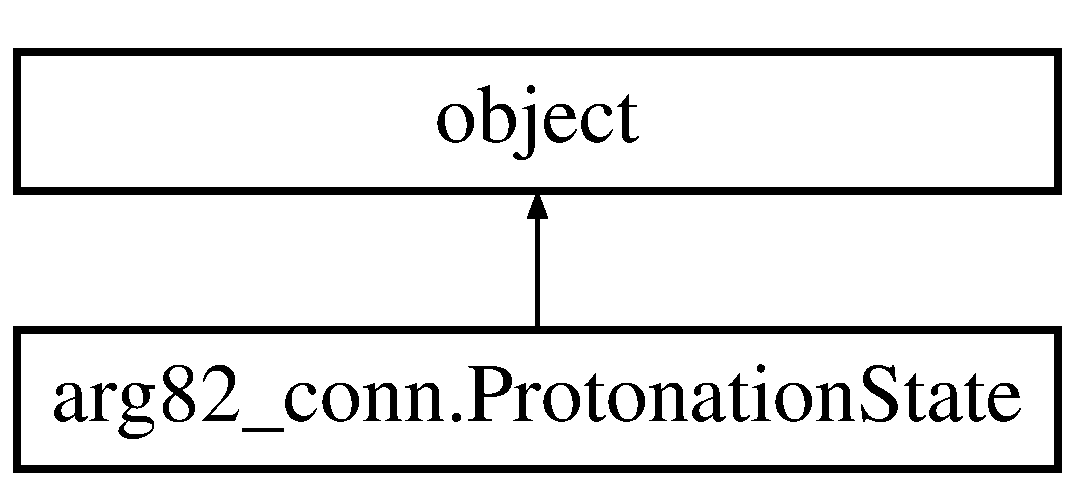
\includegraphics[height=2.000000cm]{classarg82__conn_1_1_protonation_state}
\end{center}
\end{figure}
\subsection*{Public Member Functions}
\begin{DoxyCompactItemize}
\item 
def \hyperlink{classarg82__conn_1_1_protonation_state_ae6bde57ba41f798cf046397063f1903c}{\-\_\-\-\_\-init\-\_\-\-\_\-}
\item 
def \hyperlink{classarg82__conn_1_1_protonation_state_a34715b42056818b563a4d8398e950fa4}{\-\_\-\-\_\-repr\-\_\-\-\_\-}
\item 
def \hyperlink{classarg82__conn_1_1_protonation_state_a82dadbad4de0f1f6e4b13b4ec00c6c6e}{\-\_\-\-\_\-eq\-\_\-\-\_\-}
\item 
def \hyperlink{classarg82__conn_1_1_protonation_state_a3dfdfe6af13d5d57939be5413c4247c7}{\-\_\-\-\_\-hash\-\_\-\-\_\-}
\end{DoxyCompactItemize}
\subsection*{Public Attributes}
\begin{DoxyCompactItemize}
\item 
\hyperlink{classarg82__conn_1_1_protonation_state_ae9ee5511457bf1df71f1ecf93aaa6459}{protonations}
\item 
\hyperlink{classarg82__conn_1_1_protonation_state_a9bf4fa947b0c3793b6fe44bc30136974}{energy}
\item 
\hyperlink{classarg82__conn_1_1_protonation_state_aaa69f1fdb8173e169d4d70c5246bfece}{state\-Id}
\item 
\hyperlink{classarg82__conn_1_1_protonation_state_acbb66e3f1da7f2347251a2515de60c23}{layer}
\end{DoxyCompactItemize}
\subsection*{Static Public Attributes}
\begin{DoxyCompactItemize}
\item 
list \hyperlink{classarg82__conn_1_1_protonation_state_a5d1c27726f6c948da7533e4e95f37f81}{key\-Residues} = \mbox{[}$\,$\mbox{]}
\end{DoxyCompactItemize}


\subsection{Constructor \& Destructor Documentation}
\hypertarget{classarg82__conn_1_1_protonation_state_ae6bde57ba41f798cf046397063f1903c}{\index{arg82\-\_\-conn\-::\-Protonation\-State@{arg82\-\_\-conn\-::\-Protonation\-State}!\-\_\-\-\_\-init\-\_\-\-\_\-@{\-\_\-\-\_\-init\-\_\-\-\_\-}}
\index{\-\_\-\-\_\-init\-\_\-\-\_\-@{\-\_\-\-\_\-init\-\_\-\-\_\-}!arg82_conn::ProtonationState@{arg82\-\_\-conn\-::\-Protonation\-State}}
\subsubsection[{\-\_\-\-\_\-init\-\_\-\-\_\-}]{\setlength{\rightskip}{0pt plus 5cm}def arg82\-\_\-conn.\-Protonation\-State.\-\_\-\-\_\-init\-\_\-\-\_\- (
\begin{DoxyParamCaption}
\item[{}]{self}
\end{DoxyParamCaption}
)}}\label{classarg82__conn_1_1_protonation_state_ae6bde57ba41f798cf046397063f1903c}


\subsection{Member Function Documentation}
\hypertarget{classarg82__conn_1_1_protonation_state_a82dadbad4de0f1f6e4b13b4ec00c6c6e}{\index{arg82\-\_\-conn\-::\-Protonation\-State@{arg82\-\_\-conn\-::\-Protonation\-State}!\-\_\-\-\_\-eq\-\_\-\-\_\-@{\-\_\-\-\_\-eq\-\_\-\-\_\-}}
\index{\-\_\-\-\_\-eq\-\_\-\-\_\-@{\-\_\-\-\_\-eq\-\_\-\-\_\-}!arg82_conn::ProtonationState@{arg82\-\_\-conn\-::\-Protonation\-State}}
\subsubsection[{\-\_\-\-\_\-eq\-\_\-\-\_\-}]{\setlength{\rightskip}{0pt plus 5cm}def arg82\-\_\-conn.\-Protonation\-State.\-\_\-\-\_\-eq\-\_\-\-\_\- (
\begin{DoxyParamCaption}
\item[{}]{self, }
\item[{}]{other}
\end{DoxyParamCaption}
)}}\label{classarg82__conn_1_1_protonation_state_a82dadbad4de0f1f6e4b13b4ec00c6c6e}
\hypertarget{classarg82__conn_1_1_protonation_state_a3dfdfe6af13d5d57939be5413c4247c7}{\index{arg82\-\_\-conn\-::\-Protonation\-State@{arg82\-\_\-conn\-::\-Protonation\-State}!\-\_\-\-\_\-hash\-\_\-\-\_\-@{\-\_\-\-\_\-hash\-\_\-\-\_\-}}
\index{\-\_\-\-\_\-hash\-\_\-\-\_\-@{\-\_\-\-\_\-hash\-\_\-\-\_\-}!arg82_conn::ProtonationState@{arg82\-\_\-conn\-::\-Protonation\-State}}
\subsubsection[{\-\_\-\-\_\-hash\-\_\-\-\_\-}]{\setlength{\rightskip}{0pt plus 5cm}def arg82\-\_\-conn.\-Protonation\-State.\-\_\-\-\_\-hash\-\_\-\-\_\- (
\begin{DoxyParamCaption}
\item[{}]{self}
\end{DoxyParamCaption}
)}}\label{classarg82__conn_1_1_protonation_state_a3dfdfe6af13d5d57939be5413c4247c7}
\hypertarget{classarg82__conn_1_1_protonation_state_a34715b42056818b563a4d8398e950fa4}{\index{arg82\-\_\-conn\-::\-Protonation\-State@{arg82\-\_\-conn\-::\-Protonation\-State}!\-\_\-\-\_\-repr\-\_\-\-\_\-@{\-\_\-\-\_\-repr\-\_\-\-\_\-}}
\index{\-\_\-\-\_\-repr\-\_\-\-\_\-@{\-\_\-\-\_\-repr\-\_\-\-\_\-}!arg82_conn::ProtonationState@{arg82\-\_\-conn\-::\-Protonation\-State}}
\subsubsection[{\-\_\-\-\_\-repr\-\_\-\-\_\-}]{\setlength{\rightskip}{0pt plus 5cm}def arg82\-\_\-conn.\-Protonation\-State.\-\_\-\-\_\-repr\-\_\-\-\_\- (
\begin{DoxyParamCaption}
\item[{}]{self}
\end{DoxyParamCaption}
)}}\label{classarg82__conn_1_1_protonation_state_a34715b42056818b563a4d8398e950fa4}


\subsection{Member Data Documentation}
\hypertarget{classarg82__conn_1_1_protonation_state_a9bf4fa947b0c3793b6fe44bc30136974}{\index{arg82\-\_\-conn\-::\-Protonation\-State@{arg82\-\_\-conn\-::\-Protonation\-State}!energy@{energy}}
\index{energy@{energy}!arg82_conn::ProtonationState@{arg82\-\_\-conn\-::\-Protonation\-State}}
\subsubsection[{energy}]{\setlength{\rightskip}{0pt plus 5cm}arg82\-\_\-conn.\-Protonation\-State.\-energy}}\label{classarg82__conn_1_1_protonation_state_a9bf4fa947b0c3793b6fe44bc30136974}
\hypertarget{classarg82__conn_1_1_protonation_state_a5d1c27726f6c948da7533e4e95f37f81}{\index{arg82\-\_\-conn\-::\-Protonation\-State@{arg82\-\_\-conn\-::\-Protonation\-State}!key\-Residues@{key\-Residues}}
\index{key\-Residues@{key\-Residues}!arg82_conn::ProtonationState@{arg82\-\_\-conn\-::\-Protonation\-State}}
\subsubsection[{key\-Residues}]{\setlength{\rightskip}{0pt plus 5cm}list arg82\-\_\-conn.\-Protonation\-State.\-key\-Residues = \mbox{[}$\,$\mbox{]}\hspace{0.3cm}{\ttfamily [static]}}}\label{classarg82__conn_1_1_protonation_state_a5d1c27726f6c948da7533e4e95f37f81}
\hypertarget{classarg82__conn_1_1_protonation_state_acbb66e3f1da7f2347251a2515de60c23}{\index{arg82\-\_\-conn\-::\-Protonation\-State@{arg82\-\_\-conn\-::\-Protonation\-State}!layer@{layer}}
\index{layer@{layer}!arg82_conn::ProtonationState@{arg82\-\_\-conn\-::\-Protonation\-State}}
\subsubsection[{layer}]{\setlength{\rightskip}{0pt plus 5cm}arg82\-\_\-conn.\-Protonation\-State.\-layer}}\label{classarg82__conn_1_1_protonation_state_acbb66e3f1da7f2347251a2515de60c23}
\hypertarget{classarg82__conn_1_1_protonation_state_ae9ee5511457bf1df71f1ecf93aaa6459}{\index{arg82\-\_\-conn\-::\-Protonation\-State@{arg82\-\_\-conn\-::\-Protonation\-State}!protonations@{protonations}}
\index{protonations@{protonations}!arg82_conn::ProtonationState@{arg82\-\_\-conn\-::\-Protonation\-State}}
\subsubsection[{protonations}]{\setlength{\rightskip}{0pt plus 5cm}arg82\-\_\-conn.\-Protonation\-State.\-protonations}}\label{classarg82__conn_1_1_protonation_state_ae9ee5511457bf1df71f1ecf93aaa6459}
\hypertarget{classarg82__conn_1_1_protonation_state_aaa69f1fdb8173e169d4d70c5246bfece}{\index{arg82\-\_\-conn\-::\-Protonation\-State@{arg82\-\_\-conn\-::\-Protonation\-State}!state\-Id@{state\-Id}}
\index{state\-Id@{state\-Id}!arg82_conn::ProtonationState@{arg82\-\_\-conn\-::\-Protonation\-State}}
\subsubsection[{state\-Id}]{\setlength{\rightskip}{0pt plus 5cm}arg82\-\_\-conn.\-Protonation\-State.\-state\-Id}}\label{classarg82__conn_1_1_protonation_state_aaa69f1fdb8173e169d4d70c5246bfece}


The documentation for this class was generated from the following file\-:\begin{DoxyCompactItemize}
\item 
src/scripts/hb\-\_\-connection/\hyperlink{arg82__conn_8py}{arg82\-\_\-conn.\-py}\end{DoxyCompactItemize}

\hypertarget{classget__path__barrier_1_1_protonation_state}{\section{get\-\_\-path\-\_\-barrier.\-Protonation\-State Class Reference}
\label{classget__path__barrier_1_1_protonation_state}\index{get\-\_\-path\-\_\-barrier.\-Protonation\-State@{get\-\_\-path\-\_\-barrier.\-Protonation\-State}}
}
Inheritance diagram for get\-\_\-path\-\_\-barrier.\-Protonation\-State\-:\begin{figure}[H]
\begin{center}
\leavevmode
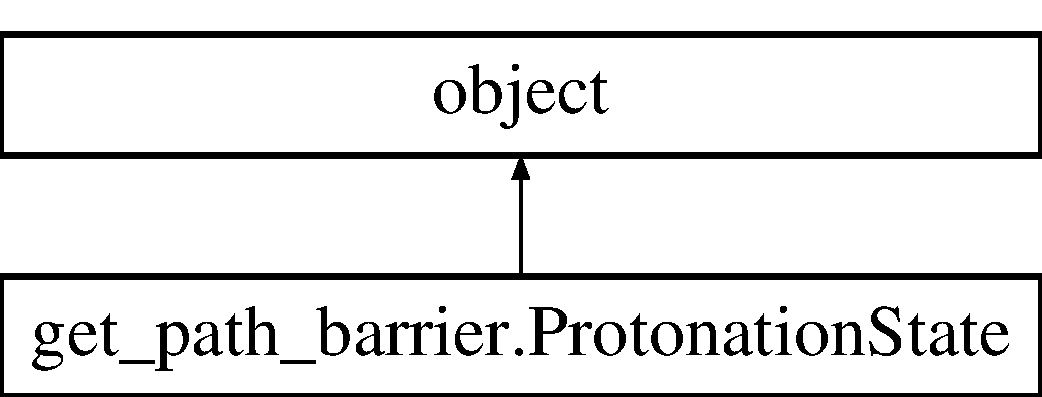
\includegraphics[height=2.000000cm]{classget__path__barrier_1_1_protonation_state}
\end{center}
\end{figure}
\subsection*{Public Member Functions}
\begin{DoxyCompactItemize}
\item 
def \hyperlink{classget__path__barrier_1_1_protonation_state_a5e56262319e3d5d2a72aa81aa0955bc9}{\-\_\-\-\_\-init\-\_\-\-\_\-}
\item 
def \hyperlink{classget__path__barrier_1_1_protonation_state_af592e055063b5b7f253725fbabe0c7ee}{\-\_\-\-\_\-repr\-\_\-\-\_\-}
\item 
def \hyperlink{classget__path__barrier_1_1_protonation_state_a37bf6b1faf41f3e5a7885153479cfc7a}{\-\_\-\-\_\-eq\-\_\-\-\_\-}
\item 
def \hyperlink{classget__path__barrier_1_1_protonation_state_ae47205464189ac09427afaafa2d490d0}{\-\_\-\-\_\-hash\-\_\-\-\_\-}
\end{DoxyCompactItemize}
\subsection*{Public Attributes}
\begin{DoxyCompactItemize}
\item 
\hyperlink{classget__path__barrier_1_1_protonation_state_ab17df337fcf1611aae2ca3d32c7d9925}{protonations}
\item 
\hyperlink{classget__path__barrier_1_1_protonation_state_a26b22fd31a45e001adadace05453862c}{energy}
\item 
\hyperlink{classget__path__barrier_1_1_protonation_state_a0887568cf1ad7ef61b03b9e9e0438186}{state\-Id}
\item 
\hyperlink{classget__path__barrier_1_1_protonation_state_afa1e7d9c2e2721bb0eaacaff5729e68f}{layer}
\end{DoxyCompactItemize}
\subsection*{Static Public Attributes}
\begin{DoxyCompactItemize}
\item 
list \hyperlink{classget__path__barrier_1_1_protonation_state_a6619f2acd36f3f2cfd1358e2912b6a97}{key\-Residues} = \mbox{[}$\,$\mbox{]}
\end{DoxyCompactItemize}


\subsection{Constructor \& Destructor Documentation}
\hypertarget{classget__path__barrier_1_1_protonation_state_a5e56262319e3d5d2a72aa81aa0955bc9}{\index{get\-\_\-path\-\_\-barrier\-::\-Protonation\-State@{get\-\_\-path\-\_\-barrier\-::\-Protonation\-State}!\-\_\-\-\_\-init\-\_\-\-\_\-@{\-\_\-\-\_\-init\-\_\-\-\_\-}}
\index{\-\_\-\-\_\-init\-\_\-\-\_\-@{\-\_\-\-\_\-init\-\_\-\-\_\-}!get_path_barrier::ProtonationState@{get\-\_\-path\-\_\-barrier\-::\-Protonation\-State}}
\subsubsection[{\-\_\-\-\_\-init\-\_\-\-\_\-}]{\setlength{\rightskip}{0pt plus 5cm}def get\-\_\-path\-\_\-barrier.\-Protonation\-State.\-\_\-\-\_\-init\-\_\-\-\_\- (
\begin{DoxyParamCaption}
\item[{}]{self}
\end{DoxyParamCaption}
)}}\label{classget__path__barrier_1_1_protonation_state_a5e56262319e3d5d2a72aa81aa0955bc9}


\subsection{Member Function Documentation}
\hypertarget{classget__path__barrier_1_1_protonation_state_a37bf6b1faf41f3e5a7885153479cfc7a}{\index{get\-\_\-path\-\_\-barrier\-::\-Protonation\-State@{get\-\_\-path\-\_\-barrier\-::\-Protonation\-State}!\-\_\-\-\_\-eq\-\_\-\-\_\-@{\-\_\-\-\_\-eq\-\_\-\-\_\-}}
\index{\-\_\-\-\_\-eq\-\_\-\-\_\-@{\-\_\-\-\_\-eq\-\_\-\-\_\-}!get_path_barrier::ProtonationState@{get\-\_\-path\-\_\-barrier\-::\-Protonation\-State}}
\subsubsection[{\-\_\-\-\_\-eq\-\_\-\-\_\-}]{\setlength{\rightskip}{0pt plus 5cm}def get\-\_\-path\-\_\-barrier.\-Protonation\-State.\-\_\-\-\_\-eq\-\_\-\-\_\- (
\begin{DoxyParamCaption}
\item[{}]{self, }
\item[{}]{other}
\end{DoxyParamCaption}
)}}\label{classget__path__barrier_1_1_protonation_state_a37bf6b1faf41f3e5a7885153479cfc7a}
\hypertarget{classget__path__barrier_1_1_protonation_state_ae47205464189ac09427afaafa2d490d0}{\index{get\-\_\-path\-\_\-barrier\-::\-Protonation\-State@{get\-\_\-path\-\_\-barrier\-::\-Protonation\-State}!\-\_\-\-\_\-hash\-\_\-\-\_\-@{\-\_\-\-\_\-hash\-\_\-\-\_\-}}
\index{\-\_\-\-\_\-hash\-\_\-\-\_\-@{\-\_\-\-\_\-hash\-\_\-\-\_\-}!get_path_barrier::ProtonationState@{get\-\_\-path\-\_\-barrier\-::\-Protonation\-State}}
\subsubsection[{\-\_\-\-\_\-hash\-\_\-\-\_\-}]{\setlength{\rightskip}{0pt plus 5cm}def get\-\_\-path\-\_\-barrier.\-Protonation\-State.\-\_\-\-\_\-hash\-\_\-\-\_\- (
\begin{DoxyParamCaption}
\item[{}]{self}
\end{DoxyParamCaption}
)}}\label{classget__path__barrier_1_1_protonation_state_ae47205464189ac09427afaafa2d490d0}
\hypertarget{classget__path__barrier_1_1_protonation_state_af592e055063b5b7f253725fbabe0c7ee}{\index{get\-\_\-path\-\_\-barrier\-::\-Protonation\-State@{get\-\_\-path\-\_\-barrier\-::\-Protonation\-State}!\-\_\-\-\_\-repr\-\_\-\-\_\-@{\-\_\-\-\_\-repr\-\_\-\-\_\-}}
\index{\-\_\-\-\_\-repr\-\_\-\-\_\-@{\-\_\-\-\_\-repr\-\_\-\-\_\-}!get_path_barrier::ProtonationState@{get\-\_\-path\-\_\-barrier\-::\-Protonation\-State}}
\subsubsection[{\-\_\-\-\_\-repr\-\_\-\-\_\-}]{\setlength{\rightskip}{0pt plus 5cm}def get\-\_\-path\-\_\-barrier.\-Protonation\-State.\-\_\-\-\_\-repr\-\_\-\-\_\- (
\begin{DoxyParamCaption}
\item[{}]{self}
\end{DoxyParamCaption}
)}}\label{classget__path__barrier_1_1_protonation_state_af592e055063b5b7f253725fbabe0c7ee}


\subsection{Member Data Documentation}
\hypertarget{classget__path__barrier_1_1_protonation_state_a26b22fd31a45e001adadace05453862c}{\index{get\-\_\-path\-\_\-barrier\-::\-Protonation\-State@{get\-\_\-path\-\_\-barrier\-::\-Protonation\-State}!energy@{energy}}
\index{energy@{energy}!get_path_barrier::ProtonationState@{get\-\_\-path\-\_\-barrier\-::\-Protonation\-State}}
\subsubsection[{energy}]{\setlength{\rightskip}{0pt plus 5cm}get\-\_\-path\-\_\-barrier.\-Protonation\-State.\-energy}}\label{classget__path__barrier_1_1_protonation_state_a26b22fd31a45e001adadace05453862c}
\hypertarget{classget__path__barrier_1_1_protonation_state_a6619f2acd36f3f2cfd1358e2912b6a97}{\index{get\-\_\-path\-\_\-barrier\-::\-Protonation\-State@{get\-\_\-path\-\_\-barrier\-::\-Protonation\-State}!key\-Residues@{key\-Residues}}
\index{key\-Residues@{key\-Residues}!get_path_barrier::ProtonationState@{get\-\_\-path\-\_\-barrier\-::\-Protonation\-State}}
\subsubsection[{key\-Residues}]{\setlength{\rightskip}{0pt plus 5cm}list get\-\_\-path\-\_\-barrier.\-Protonation\-State.\-key\-Residues = \mbox{[}$\,$\mbox{]}\hspace{0.3cm}{\ttfamily [static]}}}\label{classget__path__barrier_1_1_protonation_state_a6619f2acd36f3f2cfd1358e2912b6a97}
\hypertarget{classget__path__barrier_1_1_protonation_state_afa1e7d9c2e2721bb0eaacaff5729e68f}{\index{get\-\_\-path\-\_\-barrier\-::\-Protonation\-State@{get\-\_\-path\-\_\-barrier\-::\-Protonation\-State}!layer@{layer}}
\index{layer@{layer}!get_path_barrier::ProtonationState@{get\-\_\-path\-\_\-barrier\-::\-Protonation\-State}}
\subsubsection[{layer}]{\setlength{\rightskip}{0pt plus 5cm}get\-\_\-path\-\_\-barrier.\-Protonation\-State.\-layer}}\label{classget__path__barrier_1_1_protonation_state_afa1e7d9c2e2721bb0eaacaff5729e68f}
\hypertarget{classget__path__barrier_1_1_protonation_state_ab17df337fcf1611aae2ca3d32c7d9925}{\index{get\-\_\-path\-\_\-barrier\-::\-Protonation\-State@{get\-\_\-path\-\_\-barrier\-::\-Protonation\-State}!protonations@{protonations}}
\index{protonations@{protonations}!get_path_barrier::ProtonationState@{get\-\_\-path\-\_\-barrier\-::\-Protonation\-State}}
\subsubsection[{protonations}]{\setlength{\rightskip}{0pt plus 5cm}get\-\_\-path\-\_\-barrier.\-Protonation\-State.\-protonations}}\label{classget__path__barrier_1_1_protonation_state_ab17df337fcf1611aae2ca3d32c7d9925}
\hypertarget{classget__path__barrier_1_1_protonation_state_a0887568cf1ad7ef61b03b9e9e0438186}{\index{get\-\_\-path\-\_\-barrier\-::\-Protonation\-State@{get\-\_\-path\-\_\-barrier\-::\-Protonation\-State}!state\-Id@{state\-Id}}
\index{state\-Id@{state\-Id}!get_path_barrier::ProtonationState@{get\-\_\-path\-\_\-barrier\-::\-Protonation\-State}}
\subsubsection[{state\-Id}]{\setlength{\rightskip}{0pt plus 5cm}get\-\_\-path\-\_\-barrier.\-Protonation\-State.\-state\-Id}}\label{classget__path__barrier_1_1_protonation_state_a0887568cf1ad7ef61b03b9e9e0438186}


The documentation for this class was generated from the following file\-:\begin{DoxyCompactItemize}
\item 
src/scripts/path\-\_\-analysis/\hyperlink{get__path__barrier_8py}{get\-\_\-path\-\_\-barrier.\-py}\end{DoxyCompactItemize}

\hypertarget{classxhbpathpy_1_1protonation_state_1_1_protonation_state}{\section{xhbpathpy.\-protonation\-State.\-Protonation\-State Class Reference}
\label{classxhbpathpy_1_1protonation_state_1_1_protonation_state}\index{xhbpathpy.\-protonation\-State.\-Protonation\-State@{xhbpathpy.\-protonation\-State.\-Protonation\-State}}
}
Inheritance diagram for xhbpathpy.\-protonation\-State.\-Protonation\-State\-:\begin{figure}[H]
\begin{center}
\leavevmode
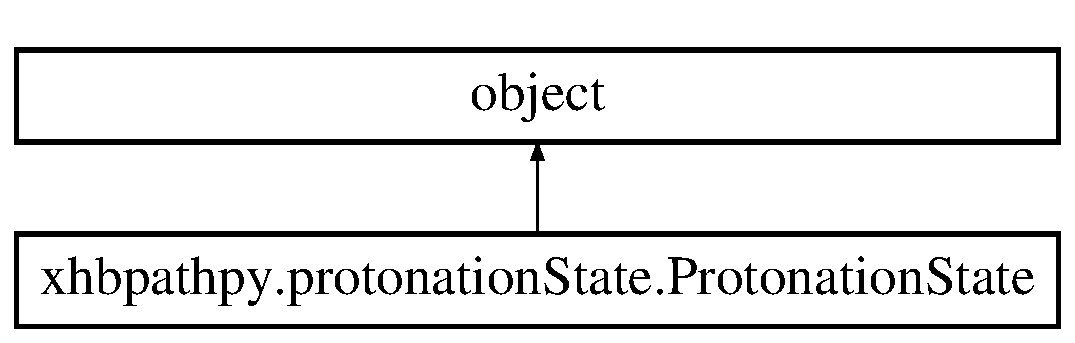
\includegraphics[height=2.000000cm]{classxhbpathpy_1_1protonation_state_1_1_protonation_state}
\end{center}
\end{figure}
\subsection*{Public Member Functions}
\begin{DoxyCompactItemize}
\item 
def \hyperlink{classxhbpathpy_1_1protonation_state_1_1_protonation_state_a97fa886feefb45c53f16de89c987ab65}{\-\_\-\-\_\-init\-\_\-\-\_\-}
\begin{DoxyCompactList}\small\item\em Constructor. \end{DoxyCompactList}\item 
def \hyperlink{classxhbpathpy_1_1protonation_state_1_1_protonation_state_a7318ae03f33e71a7a152ad302cc2d3e6}{\-\_\-\-\_\-repr\-\_\-\-\_\-}
\item 
def \hyperlink{classxhbpathpy_1_1protonation_state_1_1_protonation_state_a2d83b7c7c8bb45be4242ebaf8c4e976d}{\-\_\-\-\_\-eq\-\_\-\-\_\-}
\item 
def \hyperlink{classxhbpathpy_1_1protonation_state_1_1_protonation_state_a4d735a3c5252f4ce4bebf4f7e2b82b54}{\-\_\-\-\_\-hash\-\_\-\-\_\-}
\item 
def \hyperlink{classxhbpathpy_1_1protonation_state_1_1_protonation_state_a06d0bb021a69a624e60e4127f061ddef}{quick\-\_\-init}
\begin{DoxyCompactList}\small\item\em Quickly initialize a new protonation state. \end{DoxyCompactList}\item 
def \hyperlink{classxhbpathpy_1_1protonation_state_1_1_protonation_state_aff312c5d2ec353dc963fe1ff3bae9d61}{print\-State}
\begin{DoxyCompactList}\small\item\em Print this protonation state. \end{DoxyCompactList}\end{DoxyCompactItemize}
\subsection*{Public Attributes}
\begin{DoxyCompactItemize}
\item 
\hyperlink{classxhbpathpy_1_1protonation_state_1_1_protonation_state_af533dcbaa6d972d40c47298d04b98643}{key\-Residues}
\begin{DoxyCompactList}\small\item\em key\-Residues is of Residue type. \end{DoxyCompactList}\item 
\hyperlink{classxhbpathpy_1_1protonation_state_1_1_protonation_state_ac12c02e88c85ede9a0f32b95252c7125}{protonations}
\item 
\hyperlink{classxhbpathpy_1_1protonation_state_1_1_protonation_state_a1d139aacc9359a9d4d1302c9d847ddd2}{energy}
\item 
\hyperlink{classxhbpathpy_1_1protonation_state_1_1_protonation_state_a1b11cc48856d50aa8021f10bb598f648}{state\-Id}
\item 
\hyperlink{classxhbpathpy_1_1protonation_state_1_1_protonation_state_a03ae4323cd2c374e4d0c1ed2528e07c7}{layer}
\end{DoxyCompactItemize}


\subsection{Constructor \& Destructor Documentation}
\hypertarget{classxhbpathpy_1_1protonation_state_1_1_protonation_state_a97fa886feefb45c53f16de89c987ab65}{\index{xhbpathpy\-::protonation\-State\-::\-Protonation\-State@{xhbpathpy\-::protonation\-State\-::\-Protonation\-State}!\-\_\-\-\_\-init\-\_\-\-\_\-@{\-\_\-\-\_\-init\-\_\-\-\_\-}}
\index{\-\_\-\-\_\-init\-\_\-\-\_\-@{\-\_\-\-\_\-init\-\_\-\-\_\-}!xhbpathpy::protonationState::ProtonationState@{xhbpathpy\-::protonation\-State\-::\-Protonation\-State}}
\subsubsection[{\-\_\-\-\_\-init\-\_\-\-\_\-}]{\setlength{\rightskip}{0pt plus 5cm}def xhbpathpy.\-protonation\-State.\-Protonation\-State.\-\_\-\-\_\-init\-\_\-\-\_\- (
\begin{DoxyParamCaption}
\item[{}]{self}
\end{DoxyParamCaption}
)}}\label{classxhbpathpy_1_1protonation_state_1_1_protonation_state_a97fa886feefb45c53f16de89c987ab65}


Constructor. 



\subsection{Member Function Documentation}
\hypertarget{classxhbpathpy_1_1protonation_state_1_1_protonation_state_a2d83b7c7c8bb45be4242ebaf8c4e976d}{\index{xhbpathpy\-::protonation\-State\-::\-Protonation\-State@{xhbpathpy\-::protonation\-State\-::\-Protonation\-State}!\-\_\-\-\_\-eq\-\_\-\-\_\-@{\-\_\-\-\_\-eq\-\_\-\-\_\-}}
\index{\-\_\-\-\_\-eq\-\_\-\-\_\-@{\-\_\-\-\_\-eq\-\_\-\-\_\-}!xhbpathpy::protonationState::ProtonationState@{xhbpathpy\-::protonation\-State\-::\-Protonation\-State}}
\subsubsection[{\-\_\-\-\_\-eq\-\_\-\-\_\-}]{\setlength{\rightskip}{0pt plus 5cm}def xhbpathpy.\-protonation\-State.\-Protonation\-State.\-\_\-\-\_\-eq\-\_\-\-\_\- (
\begin{DoxyParamCaption}
\item[{}]{self, }
\item[{}]{other}
\end{DoxyParamCaption}
)}}\label{classxhbpathpy_1_1protonation_state_1_1_protonation_state_a2d83b7c7c8bb45be4242ebaf8c4e976d}
\hypertarget{classxhbpathpy_1_1protonation_state_1_1_protonation_state_a4d735a3c5252f4ce4bebf4f7e2b82b54}{\index{xhbpathpy\-::protonation\-State\-::\-Protonation\-State@{xhbpathpy\-::protonation\-State\-::\-Protonation\-State}!\-\_\-\-\_\-hash\-\_\-\-\_\-@{\-\_\-\-\_\-hash\-\_\-\-\_\-}}
\index{\-\_\-\-\_\-hash\-\_\-\-\_\-@{\-\_\-\-\_\-hash\-\_\-\-\_\-}!xhbpathpy::protonationState::ProtonationState@{xhbpathpy\-::protonation\-State\-::\-Protonation\-State}}
\subsubsection[{\-\_\-\-\_\-hash\-\_\-\-\_\-}]{\setlength{\rightskip}{0pt plus 5cm}def xhbpathpy.\-protonation\-State.\-Protonation\-State.\-\_\-\-\_\-hash\-\_\-\-\_\- (
\begin{DoxyParamCaption}
\item[{}]{self}
\end{DoxyParamCaption}
)}}\label{classxhbpathpy_1_1protonation_state_1_1_protonation_state_a4d735a3c5252f4ce4bebf4f7e2b82b54}
\hypertarget{classxhbpathpy_1_1protonation_state_1_1_protonation_state_a7318ae03f33e71a7a152ad302cc2d3e6}{\index{xhbpathpy\-::protonation\-State\-::\-Protonation\-State@{xhbpathpy\-::protonation\-State\-::\-Protonation\-State}!\-\_\-\-\_\-repr\-\_\-\-\_\-@{\-\_\-\-\_\-repr\-\_\-\-\_\-}}
\index{\-\_\-\-\_\-repr\-\_\-\-\_\-@{\-\_\-\-\_\-repr\-\_\-\-\_\-}!xhbpathpy::protonationState::ProtonationState@{xhbpathpy\-::protonation\-State\-::\-Protonation\-State}}
\subsubsection[{\-\_\-\-\_\-repr\-\_\-\-\_\-}]{\setlength{\rightskip}{0pt plus 5cm}def xhbpathpy.\-protonation\-State.\-Protonation\-State.\-\_\-\-\_\-repr\-\_\-\-\_\- (
\begin{DoxyParamCaption}
\item[{}]{self}
\end{DoxyParamCaption}
)}}\label{classxhbpathpy_1_1protonation_state_1_1_protonation_state_a7318ae03f33e71a7a152ad302cc2d3e6}
\hypertarget{classxhbpathpy_1_1protonation_state_1_1_protonation_state_aff312c5d2ec353dc963fe1ff3bae9d61}{\index{xhbpathpy\-::protonation\-State\-::\-Protonation\-State@{xhbpathpy\-::protonation\-State\-::\-Protonation\-State}!print\-State@{print\-State}}
\index{print\-State@{print\-State}!xhbpathpy::protonationState::ProtonationState@{xhbpathpy\-::protonation\-State\-::\-Protonation\-State}}
\subsubsection[{print\-State}]{\setlength{\rightskip}{0pt plus 5cm}def xhbpathpy.\-protonation\-State.\-Protonation\-State.\-print\-State (
\begin{DoxyParamCaption}
\item[{}]{self}
\end{DoxyParamCaption}
)}}\label{classxhbpathpy_1_1protonation_state_1_1_protonation_state_aff312c5d2ec353dc963fe1ff3bae9d61}


Print this protonation state. 

\hypertarget{classxhbpathpy_1_1protonation_state_1_1_protonation_state_a06d0bb021a69a624e60e4127f061ddef}{\index{xhbpathpy\-::protonation\-State\-::\-Protonation\-State@{xhbpathpy\-::protonation\-State\-::\-Protonation\-State}!quick\-\_\-init@{quick\-\_\-init}}
\index{quick\-\_\-init@{quick\-\_\-init}!xhbpathpy::protonationState::ProtonationState@{xhbpathpy\-::protonation\-State\-::\-Protonation\-State}}
\subsubsection[{quick\-\_\-init}]{\setlength{\rightskip}{0pt plus 5cm}def xhbpathpy.\-protonation\-State.\-Protonation\-State.\-quick\-\_\-init (
\begin{DoxyParamCaption}
\item[{}]{self}
\end{DoxyParamCaption}
)}}\label{classxhbpathpy_1_1protonation_state_1_1_protonation_state_a06d0bb021a69a624e60e4127f061ddef}


Quickly initialize a new protonation state. 



\subsection{Member Data Documentation}
\hypertarget{classxhbpathpy_1_1protonation_state_1_1_protonation_state_a1d139aacc9359a9d4d1302c9d847ddd2}{\index{xhbpathpy\-::protonation\-State\-::\-Protonation\-State@{xhbpathpy\-::protonation\-State\-::\-Protonation\-State}!energy@{energy}}
\index{energy@{energy}!xhbpathpy::protonationState::ProtonationState@{xhbpathpy\-::protonation\-State\-::\-Protonation\-State}}
\subsubsection[{energy}]{\setlength{\rightskip}{0pt plus 5cm}xhbpathpy.\-protonation\-State.\-Protonation\-State.\-energy}}\label{classxhbpathpy_1_1protonation_state_1_1_protonation_state_a1d139aacc9359a9d4d1302c9d847ddd2}
\hypertarget{classxhbpathpy_1_1protonation_state_1_1_protonation_state_af533dcbaa6d972d40c47298d04b98643}{\index{xhbpathpy\-::protonation\-State\-::\-Protonation\-State@{xhbpathpy\-::protonation\-State\-::\-Protonation\-State}!key\-Residues@{key\-Residues}}
\index{key\-Residues@{key\-Residues}!xhbpathpy::protonationState::ProtonationState@{xhbpathpy\-::protonation\-State\-::\-Protonation\-State}}
\subsubsection[{key\-Residues}]{\setlength{\rightskip}{0pt plus 5cm}xhbpathpy.\-protonation\-State.\-Protonation\-State.\-key\-Residues}}\label{classxhbpathpy_1_1protonation_state_1_1_protonation_state_af533dcbaa6d972d40c47298d04b98643}


key\-Residues is of Residue type. 

\hypertarget{classxhbpathpy_1_1protonation_state_1_1_protonation_state_a03ae4323cd2c374e4d0c1ed2528e07c7}{\index{xhbpathpy\-::protonation\-State\-::\-Protonation\-State@{xhbpathpy\-::protonation\-State\-::\-Protonation\-State}!layer@{layer}}
\index{layer@{layer}!xhbpathpy::protonationState::ProtonationState@{xhbpathpy\-::protonation\-State\-::\-Protonation\-State}}
\subsubsection[{layer}]{\setlength{\rightskip}{0pt plus 5cm}xhbpathpy.\-protonation\-State.\-Protonation\-State.\-layer}}\label{classxhbpathpy_1_1protonation_state_1_1_protonation_state_a03ae4323cd2c374e4d0c1ed2528e07c7}
\hypertarget{classxhbpathpy_1_1protonation_state_1_1_protonation_state_ac12c02e88c85ede9a0f32b95252c7125}{\index{xhbpathpy\-::protonation\-State\-::\-Protonation\-State@{xhbpathpy\-::protonation\-State\-::\-Protonation\-State}!protonations@{protonations}}
\index{protonations@{protonations}!xhbpathpy::protonationState::ProtonationState@{xhbpathpy\-::protonation\-State\-::\-Protonation\-State}}
\subsubsection[{protonations}]{\setlength{\rightskip}{0pt plus 5cm}xhbpathpy.\-protonation\-State.\-Protonation\-State.\-protonations}}\label{classxhbpathpy_1_1protonation_state_1_1_protonation_state_ac12c02e88c85ede9a0f32b95252c7125}
\hypertarget{classxhbpathpy_1_1protonation_state_1_1_protonation_state_a1b11cc48856d50aa8021f10bb598f648}{\index{xhbpathpy\-::protonation\-State\-::\-Protonation\-State@{xhbpathpy\-::protonation\-State\-::\-Protonation\-State}!state\-Id@{state\-Id}}
\index{state\-Id@{state\-Id}!xhbpathpy::protonationState::ProtonationState@{xhbpathpy\-::protonation\-State\-::\-Protonation\-State}}
\subsubsection[{state\-Id}]{\setlength{\rightskip}{0pt plus 5cm}xhbpathpy.\-protonation\-State.\-Protonation\-State.\-state\-Id}}\label{classxhbpathpy_1_1protonation_state_1_1_protonation_state_a1b11cc48856d50aa8021f10bb598f648}


The documentation for this class was generated from the following file\-:\begin{DoxyCompactItemize}
\item 
src/xhbpathpy/\hyperlink{protonation_state_8py}{protonation\-State.\-py}\end{DoxyCompactItemize}

\hypertarget{classhbnet_1_1_protonation_state}{\section{hbnet.\-Protonation\-State Class Reference}
\label{classhbnet_1_1_protonation_state}\index{hbnet.\-Protonation\-State@{hbnet.\-Protonation\-State}}
}
Inheritance diagram for hbnet.\-Protonation\-State\-:\begin{figure}[H]
\begin{center}
\leavevmode
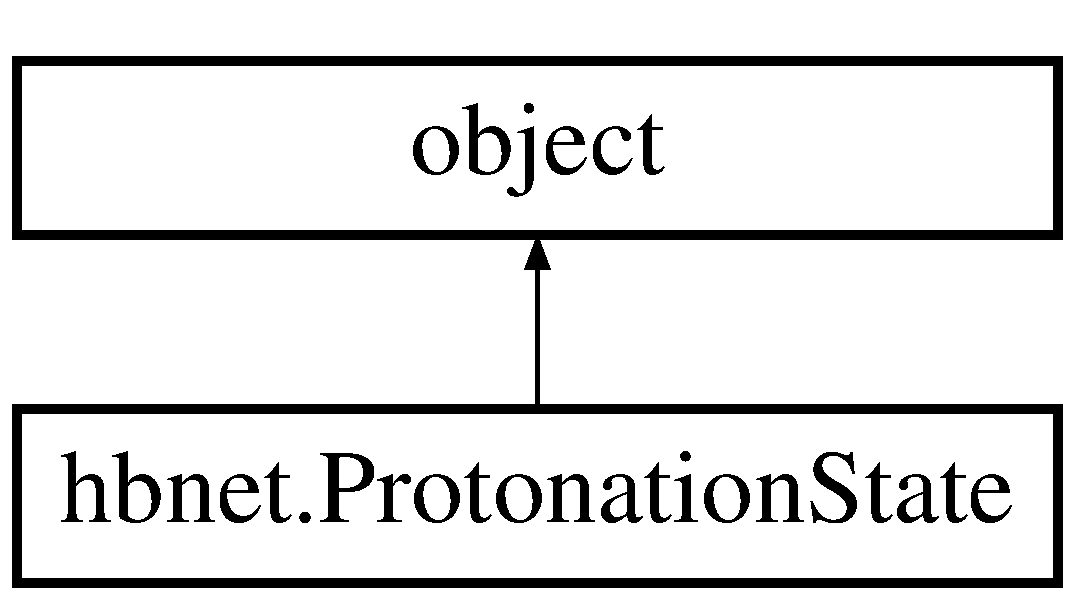
\includegraphics[height=2.000000cm]{classhbnet_1_1_protonation_state}
\end{center}
\end{figure}
\subsection*{Public Member Functions}
\begin{DoxyCompactItemize}
\item 
def \hyperlink{classhbnet_1_1_protonation_state_abdfb60e45a03e32d9886bc5ff8827691}{\-\_\-\-\_\-init\-\_\-\-\_\-}
\item 
def \hyperlink{classhbnet_1_1_protonation_state_a040bd1e1d4173a65e25cd4a9e03249bf}{\-\_\-\-\_\-repr\-\_\-\-\_\-}
\item 
def \hyperlink{classhbnet_1_1_protonation_state_a54dace9b5675cce97602e16cd5fc470d}{fine\-\_\-output}
\item 
def \hyperlink{classhbnet_1_1_protonation_state_a5f9af2e8ab2e67d0ea3c90c38314de1d}{\-\_\-\-\_\-eq\-\_\-\-\_\-}
\item 
def \hyperlink{classhbnet_1_1_protonation_state_ae8199e36ef01969fc5515c845b5fe078}{\-\_\-\-\_\-hash\-\_\-\-\_\-}
\end{DoxyCompactItemize}
\subsection*{Public Attributes}
\begin{DoxyCompactItemize}
\item 
\hyperlink{classhbnet_1_1_protonation_state_af3ba85dacb1001aaa694dd539eabfecc}{protonations}
\item 
\hyperlink{classhbnet_1_1_protonation_state_afa6daa253fcebb9a9707a139e11da56d}{energy}
\item 
\hyperlink{classhbnet_1_1_protonation_state_ad5303a482661dbcf70bce07ff287079b}{state\-Id}
\item 
\hyperlink{classhbnet_1_1_protonation_state_a1090fe1738d0d790e2e1dbf75d60249b}{layer}
\end{DoxyCompactItemize}
\subsection*{Static Public Attributes}
\begin{DoxyCompactItemize}
\item 
list \hyperlink{classhbnet_1_1_protonation_state_ab12d91a13b61409406e42e0bc32738d9}{key\-Residues} = \mbox{[}$\,$\mbox{]}
\end{DoxyCompactItemize}


\subsection{Constructor \& Destructor Documentation}
\hypertarget{classhbnet_1_1_protonation_state_abdfb60e45a03e32d9886bc5ff8827691}{\index{hbnet\-::\-Protonation\-State@{hbnet\-::\-Protonation\-State}!\-\_\-\-\_\-init\-\_\-\-\_\-@{\-\_\-\-\_\-init\-\_\-\-\_\-}}
\index{\-\_\-\-\_\-init\-\_\-\-\_\-@{\-\_\-\-\_\-init\-\_\-\-\_\-}!hbnet::ProtonationState@{hbnet\-::\-Protonation\-State}}
\subsubsection[{\-\_\-\-\_\-init\-\_\-\-\_\-}]{\setlength{\rightskip}{0pt plus 5cm}def hbnet.\-Protonation\-State.\-\_\-\-\_\-init\-\_\-\-\_\- (
\begin{DoxyParamCaption}
\item[{}]{self}
\end{DoxyParamCaption}
)}}\label{classhbnet_1_1_protonation_state_abdfb60e45a03e32d9886bc5ff8827691}


\subsection{Member Function Documentation}
\hypertarget{classhbnet_1_1_protonation_state_a5f9af2e8ab2e67d0ea3c90c38314de1d}{\index{hbnet\-::\-Protonation\-State@{hbnet\-::\-Protonation\-State}!\-\_\-\-\_\-eq\-\_\-\-\_\-@{\-\_\-\-\_\-eq\-\_\-\-\_\-}}
\index{\-\_\-\-\_\-eq\-\_\-\-\_\-@{\-\_\-\-\_\-eq\-\_\-\-\_\-}!hbnet::ProtonationState@{hbnet\-::\-Protonation\-State}}
\subsubsection[{\-\_\-\-\_\-eq\-\_\-\-\_\-}]{\setlength{\rightskip}{0pt plus 5cm}def hbnet.\-Protonation\-State.\-\_\-\-\_\-eq\-\_\-\-\_\- (
\begin{DoxyParamCaption}
\item[{}]{self, }
\item[{}]{other}
\end{DoxyParamCaption}
)}}\label{classhbnet_1_1_protonation_state_a5f9af2e8ab2e67d0ea3c90c38314de1d}
\hypertarget{classhbnet_1_1_protonation_state_ae8199e36ef01969fc5515c845b5fe078}{\index{hbnet\-::\-Protonation\-State@{hbnet\-::\-Protonation\-State}!\-\_\-\-\_\-hash\-\_\-\-\_\-@{\-\_\-\-\_\-hash\-\_\-\-\_\-}}
\index{\-\_\-\-\_\-hash\-\_\-\-\_\-@{\-\_\-\-\_\-hash\-\_\-\-\_\-}!hbnet::ProtonationState@{hbnet\-::\-Protonation\-State}}
\subsubsection[{\-\_\-\-\_\-hash\-\_\-\-\_\-}]{\setlength{\rightskip}{0pt plus 5cm}def hbnet.\-Protonation\-State.\-\_\-\-\_\-hash\-\_\-\-\_\- (
\begin{DoxyParamCaption}
\item[{}]{self}
\end{DoxyParamCaption}
)}}\label{classhbnet_1_1_protonation_state_ae8199e36ef01969fc5515c845b5fe078}
\hypertarget{classhbnet_1_1_protonation_state_a040bd1e1d4173a65e25cd4a9e03249bf}{\index{hbnet\-::\-Protonation\-State@{hbnet\-::\-Protonation\-State}!\-\_\-\-\_\-repr\-\_\-\-\_\-@{\-\_\-\-\_\-repr\-\_\-\-\_\-}}
\index{\-\_\-\-\_\-repr\-\_\-\-\_\-@{\-\_\-\-\_\-repr\-\_\-\-\_\-}!hbnet::ProtonationState@{hbnet\-::\-Protonation\-State}}
\subsubsection[{\-\_\-\-\_\-repr\-\_\-\-\_\-}]{\setlength{\rightskip}{0pt plus 5cm}def hbnet.\-Protonation\-State.\-\_\-\-\_\-repr\-\_\-\-\_\- (
\begin{DoxyParamCaption}
\item[{}]{self}
\end{DoxyParamCaption}
)}}\label{classhbnet_1_1_protonation_state_a040bd1e1d4173a65e25cd4a9e03249bf}
\hypertarget{classhbnet_1_1_protonation_state_a54dace9b5675cce97602e16cd5fc470d}{\index{hbnet\-::\-Protonation\-State@{hbnet\-::\-Protonation\-State}!fine\-\_\-output@{fine\-\_\-output}}
\index{fine\-\_\-output@{fine\-\_\-output}!hbnet::ProtonationState@{hbnet\-::\-Protonation\-State}}
\subsubsection[{fine\-\_\-output}]{\setlength{\rightskip}{0pt plus 5cm}def hbnet.\-Protonation\-State.\-fine\-\_\-output (
\begin{DoxyParamCaption}
\item[{}]{self}
\end{DoxyParamCaption}
)}}\label{classhbnet_1_1_protonation_state_a54dace9b5675cce97602e16cd5fc470d}


\subsection{Member Data Documentation}
\hypertarget{classhbnet_1_1_protonation_state_afa6daa253fcebb9a9707a139e11da56d}{\index{hbnet\-::\-Protonation\-State@{hbnet\-::\-Protonation\-State}!energy@{energy}}
\index{energy@{energy}!hbnet::ProtonationState@{hbnet\-::\-Protonation\-State}}
\subsubsection[{energy}]{\setlength{\rightskip}{0pt plus 5cm}hbnet.\-Protonation\-State.\-energy}}\label{classhbnet_1_1_protonation_state_afa6daa253fcebb9a9707a139e11da56d}
\hypertarget{classhbnet_1_1_protonation_state_ab12d91a13b61409406e42e0bc32738d9}{\index{hbnet\-::\-Protonation\-State@{hbnet\-::\-Protonation\-State}!key\-Residues@{key\-Residues}}
\index{key\-Residues@{key\-Residues}!hbnet::ProtonationState@{hbnet\-::\-Protonation\-State}}
\subsubsection[{key\-Residues}]{\setlength{\rightskip}{0pt plus 5cm}list hbnet.\-Protonation\-State.\-key\-Residues = \mbox{[}$\,$\mbox{]}\hspace{0.3cm}{\ttfamily [static]}}}\label{classhbnet_1_1_protonation_state_ab12d91a13b61409406e42e0bc32738d9}
\hypertarget{classhbnet_1_1_protonation_state_a1090fe1738d0d790e2e1dbf75d60249b}{\index{hbnet\-::\-Protonation\-State@{hbnet\-::\-Protonation\-State}!layer@{layer}}
\index{layer@{layer}!hbnet::ProtonationState@{hbnet\-::\-Protonation\-State}}
\subsubsection[{layer}]{\setlength{\rightskip}{0pt plus 5cm}hbnet.\-Protonation\-State.\-layer}}\label{classhbnet_1_1_protonation_state_a1090fe1738d0d790e2e1dbf75d60249b}
\hypertarget{classhbnet_1_1_protonation_state_af3ba85dacb1001aaa694dd539eabfecc}{\index{hbnet\-::\-Protonation\-State@{hbnet\-::\-Protonation\-State}!protonations@{protonations}}
\index{protonations@{protonations}!hbnet::ProtonationState@{hbnet\-::\-Protonation\-State}}
\subsubsection[{protonations}]{\setlength{\rightskip}{0pt plus 5cm}hbnet.\-Protonation\-State.\-protonations}}\label{classhbnet_1_1_protonation_state_af3ba85dacb1001aaa694dd539eabfecc}
\hypertarget{classhbnet_1_1_protonation_state_ad5303a482661dbcf70bce07ff287079b}{\index{hbnet\-::\-Protonation\-State@{hbnet\-::\-Protonation\-State}!state\-Id@{state\-Id}}
\index{state\-Id@{state\-Id}!hbnet::ProtonationState@{hbnet\-::\-Protonation\-State}}
\subsubsection[{state\-Id}]{\setlength{\rightskip}{0pt plus 5cm}hbnet.\-Protonation\-State.\-state\-Id}}\label{classhbnet_1_1_protonation_state_ad5303a482661dbcf70bce07ff287079b}


The documentation for this class was generated from the following file\-:\begin{DoxyCompactItemize}
\item 
src/scripts/hb\-\_\-connection/\hyperlink{hbnet_8py}{hbnet.\-py}\end{DoxyCompactItemize}

\hypertarget{classatom__hbond_1_1_res_edge}{\section{atom\-\_\-hbond.\-Res\-Edge Class Reference}
\label{classatom__hbond_1_1_res_edge}\index{atom\-\_\-hbond.\-Res\-Edge@{atom\-\_\-hbond.\-Res\-Edge}}
}
Inheritance diagram for atom\-\_\-hbond.\-Res\-Edge\-:\begin{figure}[H]
\begin{center}
\leavevmode
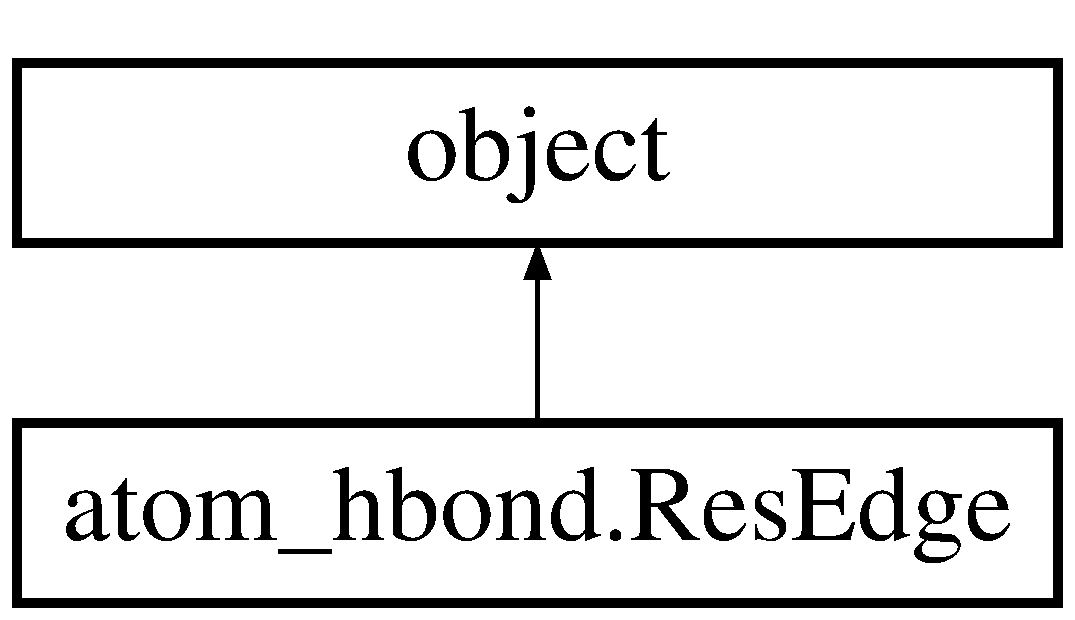
\includegraphics[height=2.000000cm]{classatom__hbond_1_1_res_edge}
\end{center}
\end{figure}
\subsection*{Public Member Functions}
\begin{DoxyCompactItemize}
\item 
def \hyperlink{classatom__hbond_1_1_res_edge_af51fd9b27e369996d2065be38e030d80}{\-\_\-\-\_\-init\-\_\-\-\_\-}
\item 
def \hyperlink{classatom__hbond_1_1_res_edge_a1b1879d61c691b05147b85a6da7b81f5}{is\-Same}
\item 
def \hyperlink{classatom__hbond_1_1_res_edge_a30c356fff77b43a187c8e0143e41c0e3}{fetch\-Nodes}
\end{DoxyCompactItemize}
\subsection*{Public Attributes}
\begin{DoxyCompactItemize}
\item 
\hyperlink{classatom__hbond_1_1_res_edge_a5a7542d9deea5ec7f8cab053e197439e}{d\-Res}
\item 
\hyperlink{classatom__hbond_1_1_res_edge_a6ba4a08bcf8e7c4f4f7ce68fd89502df}{a\-Res}
\end{DoxyCompactItemize}


\subsection{Constructor \& Destructor Documentation}
\hypertarget{classatom__hbond_1_1_res_edge_af51fd9b27e369996d2065be38e030d80}{\index{atom\-\_\-hbond\-::\-Res\-Edge@{atom\-\_\-hbond\-::\-Res\-Edge}!\-\_\-\-\_\-init\-\_\-\-\_\-@{\-\_\-\-\_\-init\-\_\-\-\_\-}}
\index{\-\_\-\-\_\-init\-\_\-\-\_\-@{\-\_\-\-\_\-init\-\_\-\-\_\-}!atom_hbond::ResEdge@{atom\-\_\-hbond\-::\-Res\-Edge}}
\subsubsection[{\-\_\-\-\_\-init\-\_\-\-\_\-}]{\setlength{\rightskip}{0pt plus 5cm}def atom\-\_\-hbond.\-Res\-Edge.\-\_\-\-\_\-init\-\_\-\-\_\- (
\begin{DoxyParamCaption}
\item[{}]{self, }
\item[{}]{d\-Res = {\ttfamily None}, }
\item[{}]{a\-Res = {\ttfamily None}}
\end{DoxyParamCaption}
)}}\label{classatom__hbond_1_1_res_edge_af51fd9b27e369996d2065be38e030d80}


\subsection{Member Function Documentation}
\hypertarget{classatom__hbond_1_1_res_edge_a30c356fff77b43a187c8e0143e41c0e3}{\index{atom\-\_\-hbond\-::\-Res\-Edge@{atom\-\_\-hbond\-::\-Res\-Edge}!fetch\-Nodes@{fetch\-Nodes}}
\index{fetch\-Nodes@{fetch\-Nodes}!atom_hbond::ResEdge@{atom\-\_\-hbond\-::\-Res\-Edge}}
\subsubsection[{fetch\-Nodes}]{\setlength{\rightskip}{0pt plus 5cm}def atom\-\_\-hbond.\-Res\-Edge.\-fetch\-Nodes (
\begin{DoxyParamCaption}
\item[{}]{self}
\end{DoxyParamCaption}
)}}\label{classatom__hbond_1_1_res_edge_a30c356fff77b43a187c8e0143e41c0e3}
\hypertarget{classatom__hbond_1_1_res_edge_a1b1879d61c691b05147b85a6da7b81f5}{\index{atom\-\_\-hbond\-::\-Res\-Edge@{atom\-\_\-hbond\-::\-Res\-Edge}!is\-Same@{is\-Same}}
\index{is\-Same@{is\-Same}!atom_hbond::ResEdge@{atom\-\_\-hbond\-::\-Res\-Edge}}
\subsubsection[{is\-Same}]{\setlength{\rightskip}{0pt plus 5cm}def atom\-\_\-hbond.\-Res\-Edge.\-is\-Same (
\begin{DoxyParamCaption}
\item[{}]{self, }
\item[{}]{other}
\end{DoxyParamCaption}
)}}\label{classatom__hbond_1_1_res_edge_a1b1879d61c691b05147b85a6da7b81f5}


\subsection{Member Data Documentation}
\hypertarget{classatom__hbond_1_1_res_edge_a6ba4a08bcf8e7c4f4f7ce68fd89502df}{\index{atom\-\_\-hbond\-::\-Res\-Edge@{atom\-\_\-hbond\-::\-Res\-Edge}!a\-Res@{a\-Res}}
\index{a\-Res@{a\-Res}!atom_hbond::ResEdge@{atom\-\_\-hbond\-::\-Res\-Edge}}
\subsubsection[{a\-Res}]{\setlength{\rightskip}{0pt plus 5cm}atom\-\_\-hbond.\-Res\-Edge.\-a\-Res}}\label{classatom__hbond_1_1_res_edge_a6ba4a08bcf8e7c4f4f7ce68fd89502df}
\hypertarget{classatom__hbond_1_1_res_edge_a5a7542d9deea5ec7f8cab053e197439e}{\index{atom\-\_\-hbond\-::\-Res\-Edge@{atom\-\_\-hbond\-::\-Res\-Edge}!d\-Res@{d\-Res}}
\index{d\-Res@{d\-Res}!atom_hbond::ResEdge@{atom\-\_\-hbond\-::\-Res\-Edge}}
\subsubsection[{d\-Res}]{\setlength{\rightskip}{0pt plus 5cm}atom\-\_\-hbond.\-Res\-Edge.\-d\-Res}}\label{classatom__hbond_1_1_res_edge_a5a7542d9deea5ec7f8cab053e197439e}


The documentation for this class was generated from the following file\-:\begin{DoxyCompactItemize}
\item 
src/scripts/hb\-\_\-connection/\hyperlink{atom__hbond_8py}{atom\-\_\-hbond.\-py}\end{DoxyCompactItemize}

\hypertarget{classxmccepy_1_1mp_1_1_r_e_s_i_d_u_e}{\section{xmccepy.\-mp.\-R\-E\-S\-I\-D\-U\-E Class Reference}
\label{classxmccepy_1_1mp_1_1_r_e_s_i_d_u_e}\index{xmccepy.\-mp.\-R\-E\-S\-I\-D\-U\-E@{xmccepy.\-mp.\-R\-E\-S\-I\-D\-U\-E}}
}
\subsection*{Public Member Functions}
\begin{DoxyCompactItemize}
\item 
def \hyperlink{classxmccepy_1_1mp_1_1_r_e_s_i_d_u_e_a85b80421d52d6f2fc6a6ebce9e24718b}{\-\_\-\-\_\-init\-\_\-\-\_\-}
\end{DoxyCompactItemize}
\subsection*{Public Attributes}
\begin{DoxyCompactItemize}
\item 
\hyperlink{classxmccepy_1_1mp_1_1_r_e_s_i_d_u_e_a9e276df72d318575591218b210b21ab2}{confs}
\end{DoxyCompactItemize}


\subsection{Constructor \& Destructor Documentation}
\hypertarget{classxmccepy_1_1mp_1_1_r_e_s_i_d_u_e_a85b80421d52d6f2fc6a6ebce9e24718b}{\index{xmccepy\-::mp\-::\-R\-E\-S\-I\-D\-U\-E@{xmccepy\-::mp\-::\-R\-E\-S\-I\-D\-U\-E}!\-\_\-\-\_\-init\-\_\-\-\_\-@{\-\_\-\-\_\-init\-\_\-\-\_\-}}
\index{\-\_\-\-\_\-init\-\_\-\-\_\-@{\-\_\-\-\_\-init\-\_\-\-\_\-}!xmccepy::mp::RESIDUE@{xmccepy\-::mp\-::\-R\-E\-S\-I\-D\-U\-E}}
\subsubsection[{\-\_\-\-\_\-init\-\_\-\-\_\-}]{\setlength{\rightskip}{0pt plus 5cm}def xmccepy.\-mp.\-R\-E\-S\-I\-D\-U\-E.\-\_\-\-\_\-init\-\_\-\-\_\- (
\begin{DoxyParamCaption}
\item[{}]{self}
\end{DoxyParamCaption}
)}}\label{classxmccepy_1_1mp_1_1_r_e_s_i_d_u_e_a85b80421d52d6f2fc6a6ebce9e24718b}


\subsection{Member Data Documentation}
\hypertarget{classxmccepy_1_1mp_1_1_r_e_s_i_d_u_e_a9e276df72d318575591218b210b21ab2}{\index{xmccepy\-::mp\-::\-R\-E\-S\-I\-D\-U\-E@{xmccepy\-::mp\-::\-R\-E\-S\-I\-D\-U\-E}!confs@{confs}}
\index{confs@{confs}!xmccepy::mp::RESIDUE@{xmccepy\-::mp\-::\-R\-E\-S\-I\-D\-U\-E}}
\subsubsection[{confs}]{\setlength{\rightskip}{0pt plus 5cm}xmccepy.\-mp.\-R\-E\-S\-I\-D\-U\-E.\-confs}}\label{classxmccepy_1_1mp_1_1_r_e_s_i_d_u_e_a9e276df72d318575591218b210b21ab2}


The documentation for this class was generated from the following file\-:\begin{DoxyCompactItemize}
\item 
src/xmccepy/\hyperlink{mp_8py}{mp.\-py}\end{DoxyCompactItemize}

\hypertarget{classxmccepy_1_1residue_1_1_residue}{\section{xmccepy.\-residue.\-Residue Class Reference}
\label{classxmccepy_1_1residue_1_1_residue}\index{xmccepy.\-residue.\-Residue@{xmccepy.\-residue.\-Residue}}
}


Created on Apr 1, 2014.  


Inheritance diagram for xmccepy.\-residue.\-Residue\-:\begin{figure}[H]
\begin{center}
\leavevmode
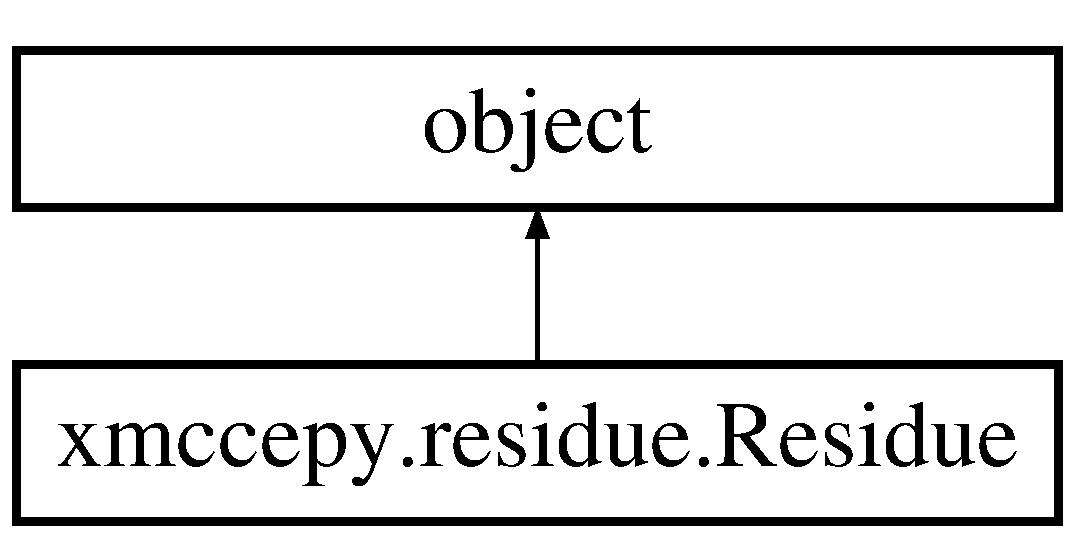
\includegraphics[height=2.000000cm]{classxmccepy_1_1residue_1_1_residue}
\end{center}
\end{figure}
\subsection*{Public Member Functions}
\begin{DoxyCompactItemize}
\item 
def \hyperlink{classxmccepy_1_1residue_1_1_residue_ab61144d8c5aed99cc706225b17e9ac03}{\-\_\-\-\_\-init\-\_\-\-\_\-}
\begin{DoxyCompactList}\small\item\em Constructor. \end{DoxyCompactList}\end{DoxyCompactItemize}
\subsection*{Public Attributes}
\begin{DoxyCompactItemize}
\item 
\hyperlink{classxmccepy_1_1residue_1_1_residue_a07eb4b463b514b1f1e86d03a6ff02a98}{res\-Name}
\item 
\hyperlink{classxmccepy_1_1residue_1_1_residue_afdd072f15f2fa5640bd67e0e5f6eb1de}{chain\-Id}
\end{DoxyCompactItemize}


\subsection{Detailed Description}
Created on Apr 1, 2014. 

\begin{DoxyAuthor}{Author}
\-: xzhu \begin{DoxyVerb}Residue class.\end{DoxyVerb}
 
\end{DoxyAuthor}


\subsection{Constructor \& Destructor Documentation}
\hypertarget{classxmccepy_1_1residue_1_1_residue_ab61144d8c5aed99cc706225b17e9ac03}{\index{xmccepy\-::residue\-::\-Residue@{xmccepy\-::residue\-::\-Residue}!\-\_\-\-\_\-init\-\_\-\-\_\-@{\-\_\-\-\_\-init\-\_\-\-\_\-}}
\index{\-\_\-\-\_\-init\-\_\-\-\_\-@{\-\_\-\-\_\-init\-\_\-\-\_\-}!xmccepy::residue::Residue@{xmccepy\-::residue\-::\-Residue}}
\subsubsection[{\-\_\-\-\_\-init\-\_\-\-\_\-}]{\setlength{\rightskip}{0pt plus 5cm}def xmccepy.\-residue.\-Residue.\-\_\-\-\_\-init\-\_\-\-\_\- (
\begin{DoxyParamCaption}
\item[{}]{self}
\end{DoxyParamCaption}
)}}\label{classxmccepy_1_1residue_1_1_residue_ab61144d8c5aed99cc706225b17e9ac03}


Constructor. 



\subsection{Member Data Documentation}
\hypertarget{classxmccepy_1_1residue_1_1_residue_afdd072f15f2fa5640bd67e0e5f6eb1de}{\index{xmccepy\-::residue\-::\-Residue@{xmccepy\-::residue\-::\-Residue}!chain\-Id@{chain\-Id}}
\index{chain\-Id@{chain\-Id}!xmccepy::residue::Residue@{xmccepy\-::residue\-::\-Residue}}
\subsubsection[{chain\-Id}]{\setlength{\rightskip}{0pt plus 5cm}xmccepy.\-residue.\-Residue.\-chain\-Id}}\label{classxmccepy_1_1residue_1_1_residue_afdd072f15f2fa5640bd67e0e5f6eb1de}
\hypertarget{classxmccepy_1_1residue_1_1_residue_a07eb4b463b514b1f1e86d03a6ff02a98}{\index{xmccepy\-::residue\-::\-Residue@{xmccepy\-::residue\-::\-Residue}!res\-Name@{res\-Name}}
\index{res\-Name@{res\-Name}!xmccepy::residue::Residue@{xmccepy\-::residue\-::\-Residue}}
\subsubsection[{res\-Name}]{\setlength{\rightskip}{0pt plus 5cm}xmccepy.\-residue.\-Residue.\-res\-Name}}\label{classxmccepy_1_1residue_1_1_residue_a07eb4b463b514b1f1e86d03a6ff02a98}


The documentation for this class was generated from the following file\-:\begin{DoxyCompactItemize}
\item 
src/xmccepy/\hyperlink{residue_8py}{residue.\-py}\end{DoxyCompactItemize}

\hypertarget{classatom__hbond_1_1_res_node}{\section{atom\-\_\-hbond.\-Res\-Node Class Reference}
\label{classatom__hbond_1_1_res_node}\index{atom\-\_\-hbond.\-Res\-Node@{atom\-\_\-hbond.\-Res\-Node}}
}
Inheritance diagram for atom\-\_\-hbond.\-Res\-Node\-:\begin{figure}[H]
\begin{center}
\leavevmode
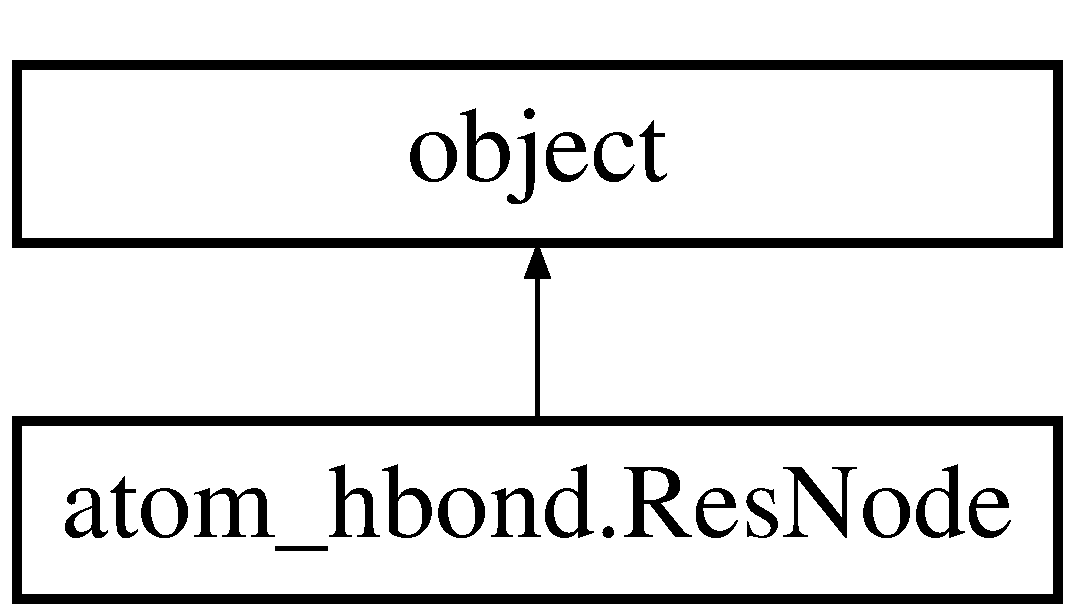
\includegraphics[height=2.000000cm]{classatom__hbond_1_1_res_node}
\end{center}
\end{figure}
\subsection*{Public Member Functions}
\begin{DoxyCompactItemize}
\item 
def \hyperlink{classatom__hbond_1_1_res_node_ad7da22ae1c6d68364e571b7b7f818cb1}{\-\_\-\-\_\-init\-\_\-\-\_\-}
\item 
def \hyperlink{classatom__hbond_1_1_res_node_a7d4b9aa1d615f1fdf7e1716948404b1a}{is\-Same}
\item 
def \hyperlink{classatom__hbond_1_1_res_node_a20413704596e1f492a2056602b759742}{\-\_\-\-\_\-repr\-\_\-\-\_\-}
\item 
def \hyperlink{classatom__hbond_1_1_res_node_a0b6c7a0f083bd384e039b09a7cf560a1}{\-\_\-\-\_\-eq\-\_\-\-\_\-}
\item 
def \hyperlink{classatom__hbond_1_1_res_node_a968af5a70cdc58c12b5d72908ba164f4}{\-\_\-\-\_\-hash\-\_\-\-\_\-}
\end{DoxyCompactItemize}
\subsection*{Public Attributes}
\begin{DoxyCompactItemize}
\item 
\hyperlink{classatom__hbond_1_1_res_node_ae1e370985c9c26c01024a282747c3585}{res\-Name}
\item 
\hyperlink{classatom__hbond_1_1_res_node_a21a674e4aa679f046f032954a4c4a254}{atom\-Name}
\end{DoxyCompactItemize}


\subsection{Constructor \& Destructor Documentation}
\hypertarget{classatom__hbond_1_1_res_node_ad7da22ae1c6d68364e571b7b7f818cb1}{\index{atom\-\_\-hbond\-::\-Res\-Node@{atom\-\_\-hbond\-::\-Res\-Node}!\-\_\-\-\_\-init\-\_\-\-\_\-@{\-\_\-\-\_\-init\-\_\-\-\_\-}}
\index{\-\_\-\-\_\-init\-\_\-\-\_\-@{\-\_\-\-\_\-init\-\_\-\-\_\-}!atom_hbond::ResNode@{atom\-\_\-hbond\-::\-Res\-Node}}
\subsubsection[{\-\_\-\-\_\-init\-\_\-\-\_\-}]{\setlength{\rightskip}{0pt plus 5cm}def atom\-\_\-hbond.\-Res\-Node.\-\_\-\-\_\-init\-\_\-\-\_\- (
\begin{DoxyParamCaption}
\item[{}]{self, }
\item[{}]{r\-Name = {\ttfamily \char`\"{}\char`\"{}}, }
\item[{}]{a\-Name = {\ttfamily \char`\"{}\char`\"{}}}
\end{DoxyParamCaption}
)}}\label{classatom__hbond_1_1_res_node_ad7da22ae1c6d68364e571b7b7f818cb1}


\subsection{Member Function Documentation}
\hypertarget{classatom__hbond_1_1_res_node_a0b6c7a0f083bd384e039b09a7cf560a1}{\index{atom\-\_\-hbond\-::\-Res\-Node@{atom\-\_\-hbond\-::\-Res\-Node}!\-\_\-\-\_\-eq\-\_\-\-\_\-@{\-\_\-\-\_\-eq\-\_\-\-\_\-}}
\index{\-\_\-\-\_\-eq\-\_\-\-\_\-@{\-\_\-\-\_\-eq\-\_\-\-\_\-}!atom_hbond::ResNode@{atom\-\_\-hbond\-::\-Res\-Node}}
\subsubsection[{\-\_\-\-\_\-eq\-\_\-\-\_\-}]{\setlength{\rightskip}{0pt plus 5cm}def atom\-\_\-hbond.\-Res\-Node.\-\_\-\-\_\-eq\-\_\-\-\_\- (
\begin{DoxyParamCaption}
\item[{}]{self, }
\item[{}]{other}
\end{DoxyParamCaption}
)}}\label{classatom__hbond_1_1_res_node_a0b6c7a0f083bd384e039b09a7cf560a1}
\hypertarget{classatom__hbond_1_1_res_node_a968af5a70cdc58c12b5d72908ba164f4}{\index{atom\-\_\-hbond\-::\-Res\-Node@{atom\-\_\-hbond\-::\-Res\-Node}!\-\_\-\-\_\-hash\-\_\-\-\_\-@{\-\_\-\-\_\-hash\-\_\-\-\_\-}}
\index{\-\_\-\-\_\-hash\-\_\-\-\_\-@{\-\_\-\-\_\-hash\-\_\-\-\_\-}!atom_hbond::ResNode@{atom\-\_\-hbond\-::\-Res\-Node}}
\subsubsection[{\-\_\-\-\_\-hash\-\_\-\-\_\-}]{\setlength{\rightskip}{0pt plus 5cm}def atom\-\_\-hbond.\-Res\-Node.\-\_\-\-\_\-hash\-\_\-\-\_\- (
\begin{DoxyParamCaption}
\item[{}]{self}
\end{DoxyParamCaption}
)}}\label{classatom__hbond_1_1_res_node_a968af5a70cdc58c12b5d72908ba164f4}
\hypertarget{classatom__hbond_1_1_res_node_a20413704596e1f492a2056602b759742}{\index{atom\-\_\-hbond\-::\-Res\-Node@{atom\-\_\-hbond\-::\-Res\-Node}!\-\_\-\-\_\-repr\-\_\-\-\_\-@{\-\_\-\-\_\-repr\-\_\-\-\_\-}}
\index{\-\_\-\-\_\-repr\-\_\-\-\_\-@{\-\_\-\-\_\-repr\-\_\-\-\_\-}!atom_hbond::ResNode@{atom\-\_\-hbond\-::\-Res\-Node}}
\subsubsection[{\-\_\-\-\_\-repr\-\_\-\-\_\-}]{\setlength{\rightskip}{0pt plus 5cm}def atom\-\_\-hbond.\-Res\-Node.\-\_\-\-\_\-repr\-\_\-\-\_\- (
\begin{DoxyParamCaption}
\item[{}]{self}
\end{DoxyParamCaption}
)}}\label{classatom__hbond_1_1_res_node_a20413704596e1f492a2056602b759742}
\hypertarget{classatom__hbond_1_1_res_node_a7d4b9aa1d615f1fdf7e1716948404b1a}{\index{atom\-\_\-hbond\-::\-Res\-Node@{atom\-\_\-hbond\-::\-Res\-Node}!is\-Same@{is\-Same}}
\index{is\-Same@{is\-Same}!atom_hbond::ResNode@{atom\-\_\-hbond\-::\-Res\-Node}}
\subsubsection[{is\-Same}]{\setlength{\rightskip}{0pt plus 5cm}def atom\-\_\-hbond.\-Res\-Node.\-is\-Same (
\begin{DoxyParamCaption}
\item[{}]{self, }
\item[{}]{other}
\end{DoxyParamCaption}
)}}\label{classatom__hbond_1_1_res_node_a7d4b9aa1d615f1fdf7e1716948404b1a}


\subsection{Member Data Documentation}
\hypertarget{classatom__hbond_1_1_res_node_a21a674e4aa679f046f032954a4c4a254}{\index{atom\-\_\-hbond\-::\-Res\-Node@{atom\-\_\-hbond\-::\-Res\-Node}!atom\-Name@{atom\-Name}}
\index{atom\-Name@{atom\-Name}!atom_hbond::ResNode@{atom\-\_\-hbond\-::\-Res\-Node}}
\subsubsection[{atom\-Name}]{\setlength{\rightskip}{0pt plus 5cm}atom\-\_\-hbond.\-Res\-Node.\-atom\-Name}}\label{classatom__hbond_1_1_res_node_a21a674e4aa679f046f032954a4c4a254}
\hypertarget{classatom__hbond_1_1_res_node_ae1e370985c9c26c01024a282747c3585}{\index{atom\-\_\-hbond\-::\-Res\-Node@{atom\-\_\-hbond\-::\-Res\-Node}!res\-Name@{res\-Name}}
\index{res\-Name@{res\-Name}!atom_hbond::ResNode@{atom\-\_\-hbond\-::\-Res\-Node}}
\subsubsection[{res\-Name}]{\setlength{\rightskip}{0pt plus 5cm}atom\-\_\-hbond.\-Res\-Node.\-res\-Name}}\label{classatom__hbond_1_1_res_node_ae1e370985c9c26c01024a282747c3585}


The documentation for this class was generated from the following file\-:\begin{DoxyCompactItemize}
\item 
src/scripts/hb\-\_\-connection/\hyperlink{atom__hbond_8py}{atom\-\_\-hbond.\-py}\end{DoxyCompactItemize}

\hypertarget{classget__charge_1_1_res_pro}{\section{get\-\_\-charge.\-Res\-Pro Class Reference}
\label{classget__charge_1_1_res_pro}\index{get\-\_\-charge.\-Res\-Pro@{get\-\_\-charge.\-Res\-Pro}}
}


Get the charges of residues.  


Inheritance diagram for get\-\_\-charge.\-Res\-Pro\-:\begin{figure}[H]
\begin{center}
\leavevmode
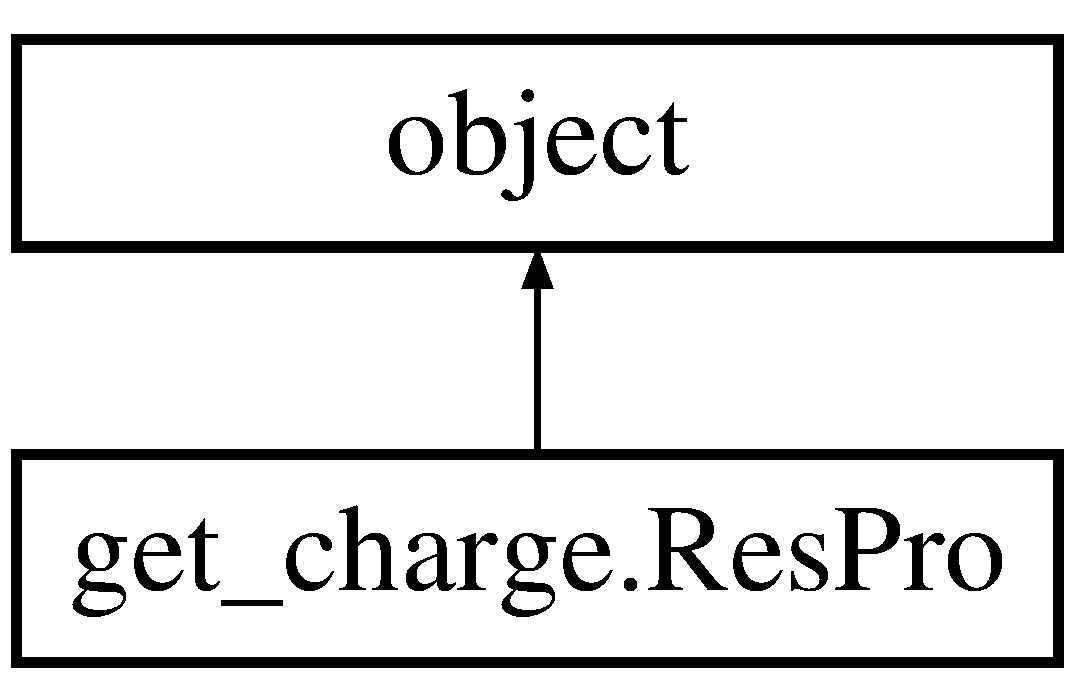
\includegraphics[height=2.000000cm]{classget__charge_1_1_res_pro}
\end{center}
\end{figure}
\subsection*{Public Member Functions}
\begin{DoxyCompactItemize}
\item 
def \hyperlink{classget__charge_1_1_res_pro_a0a1c975f9bb2ba10abe7c9f4be965b04}{\-\_\-\-\_\-init\-\_\-\-\_\-}
\item 
def \hyperlink{classget__charge_1_1_res_pro_aa0b4bed643d3d032ed97c89f5426cfef}{\-\_\-\-\_\-str\-\_\-\-\_\-}
\item 
def \hyperlink{classget__charge_1_1_res_pro_a2ff72116a5eec8e96c3085269e265250}{get\-Stat}
\end{DoxyCompactItemize}
\subsection*{Public Attributes}
\begin{DoxyCompactItemize}
\item 
\hyperlink{classget__charge_1_1_res_pro_aaa9de483c5f88fe49fd682dd1b8a62e7}{charges}
\item 
\hyperlink{classget__charge_1_1_res_pro_af00fc3f5bae5c3d3734b384b2d2c466d}{r\-Name}
\item 
\hyperlink{classget__charge_1_1_res_pro_a19649fb10b2d365eddf247107e39b0d0}{avg}
\item 
\hyperlink{classget__charge_1_1_res_pro_afad79b4ab35532abe9a7d305725fb0bc}{std}
\item 
\hyperlink{classget__charge_1_1_res_pro_a0f70c65e6cef508bcd63147ad7265fee}{protonation}
\end{DoxyCompactItemize}
\subsection*{Static Public Attributes}
\begin{DoxyCompactItemize}
\item 
tuple \hyperlink{classget__charge_1_1_res_pro_a19f4f7319d0e78071cad89e477d96f9f}{all\-Run\-Types} = (\char`\"{}cqr\char`\"{}, \char`\"{}cql\char`\"{}, \char`\"{}cdr\char`\"{}, \char`\"{}cdl\char`\"{}, \char`\"{}hqr\char`\"{}, \char`\"{}hql\char`\"{}, \char`\"{}hdr\char`\"{}, \char`\"{}hdl\char`\"{})
\item 
string \hyperlink{classget__charge_1_1_res_pro_a6abe27b9c2d55e6f735eb1afe0a83916}{D\-E\-F\-A\-U\-L\-T\-\_\-\-C\-R\-G} = \char`\"{}na\char`\"{}
\end{DoxyCompactItemize}
\subsection*{Static Private Attributes}
\begin{DoxyCompactItemize}
\item 
\hyperlink{classget__charge_1_1_res_pro_a2d6a3912943f7b858e8b5f04231c3420}{\-\_\-\-\_\-repr\-\_\-\-\_\-} = \hyperlink{classget__charge_1_1_res_pro_aa0b4bed643d3d032ed97c89f5426cfef}{\-\_\-\-\_\-str\-\_\-\-\_\-}
\end{DoxyCompactItemize}


\subsection{Detailed Description}
Get the charges of residues. 

It's similar to the script \char`\"{}collect\-\_\-crg.\-py\char`\"{}. 

\subsection{Constructor \& Destructor Documentation}
\hypertarget{classget__charge_1_1_res_pro_a0a1c975f9bb2ba10abe7c9f4be965b04}{\index{get\-\_\-charge\-::\-Res\-Pro@{get\-\_\-charge\-::\-Res\-Pro}!\-\_\-\-\_\-init\-\_\-\-\_\-@{\-\_\-\-\_\-init\-\_\-\-\_\-}}
\index{\-\_\-\-\_\-init\-\_\-\-\_\-@{\-\_\-\-\_\-init\-\_\-\-\_\-}!get_charge::ResPro@{get\-\_\-charge\-::\-Res\-Pro}}
\subsubsection[{\-\_\-\-\_\-init\-\_\-\-\_\-}]{\setlength{\rightskip}{0pt plus 5cm}def get\-\_\-charge.\-Res\-Pro.\-\_\-\-\_\-init\-\_\-\-\_\- (
\begin{DoxyParamCaption}
\item[{}]{self, }
\item[{}]{name = {\ttfamily ''}}
\end{DoxyParamCaption}
)}}\label{classget__charge_1_1_res_pro_a0a1c975f9bb2ba10abe7c9f4be965b04}


\subsection{Member Function Documentation}
\hypertarget{classget__charge_1_1_res_pro_aa0b4bed643d3d032ed97c89f5426cfef}{\index{get\-\_\-charge\-::\-Res\-Pro@{get\-\_\-charge\-::\-Res\-Pro}!\-\_\-\-\_\-str\-\_\-\-\_\-@{\-\_\-\-\_\-str\-\_\-\-\_\-}}
\index{\-\_\-\-\_\-str\-\_\-\-\_\-@{\-\_\-\-\_\-str\-\_\-\-\_\-}!get_charge::ResPro@{get\-\_\-charge\-::\-Res\-Pro}}
\subsubsection[{\-\_\-\-\_\-str\-\_\-\-\_\-}]{\setlength{\rightskip}{0pt plus 5cm}def get\-\_\-charge.\-Res\-Pro.\-\_\-\-\_\-str\-\_\-\-\_\- (
\begin{DoxyParamCaption}
\item[{}]{self}
\end{DoxyParamCaption}
)}}\label{classget__charge_1_1_res_pro_aa0b4bed643d3d032ed97c89f5426cfef}
\hypertarget{classget__charge_1_1_res_pro_a2ff72116a5eec8e96c3085269e265250}{\index{get\-\_\-charge\-::\-Res\-Pro@{get\-\_\-charge\-::\-Res\-Pro}!get\-Stat@{get\-Stat}}
\index{get\-Stat@{get\-Stat}!get_charge::ResPro@{get\-\_\-charge\-::\-Res\-Pro}}
\subsubsection[{get\-Stat}]{\setlength{\rightskip}{0pt plus 5cm}def get\-\_\-charge.\-Res\-Pro.\-get\-Stat (
\begin{DoxyParamCaption}
\item[{}]{self}
\end{DoxyParamCaption}
)}}\label{classget__charge_1_1_res_pro_a2ff72116a5eec8e96c3085269e265250}


\subsection{Member Data Documentation}
\hypertarget{classget__charge_1_1_res_pro_a2d6a3912943f7b858e8b5f04231c3420}{\index{get\-\_\-charge\-::\-Res\-Pro@{get\-\_\-charge\-::\-Res\-Pro}!\-\_\-\-\_\-repr\-\_\-\-\_\-@{\-\_\-\-\_\-repr\-\_\-\-\_\-}}
\index{\-\_\-\-\_\-repr\-\_\-\-\_\-@{\-\_\-\-\_\-repr\-\_\-\-\_\-}!get_charge::ResPro@{get\-\_\-charge\-::\-Res\-Pro}}
\subsubsection[{\-\_\-\-\_\-repr\-\_\-\-\_\-}]{\setlength{\rightskip}{0pt plus 5cm}get\-\_\-charge.\-Res\-Pro.\-\_\-\-\_\-repr\-\_\-\-\_\- = {\bf \-\_\-\-\_\-str\-\_\-\-\_\-}\hspace{0.3cm}{\ttfamily [static]}, {\ttfamily [private]}}}\label{classget__charge_1_1_res_pro_a2d6a3912943f7b858e8b5f04231c3420}
\hypertarget{classget__charge_1_1_res_pro_a19f4f7319d0e78071cad89e477d96f9f}{\index{get\-\_\-charge\-::\-Res\-Pro@{get\-\_\-charge\-::\-Res\-Pro}!all\-Run\-Types@{all\-Run\-Types}}
\index{all\-Run\-Types@{all\-Run\-Types}!get_charge::ResPro@{get\-\_\-charge\-::\-Res\-Pro}}
\subsubsection[{all\-Run\-Types}]{\setlength{\rightskip}{0pt plus 5cm}tuple get\-\_\-charge.\-Res\-Pro.\-all\-Run\-Types = (\char`\"{}cqr\char`\"{}, \char`\"{}cql\char`\"{}, \char`\"{}cdr\char`\"{}, \char`\"{}cdl\char`\"{}, \char`\"{}hqr\char`\"{}, \char`\"{}hql\char`\"{}, \char`\"{}hdr\char`\"{}, \char`\"{}hdl\char`\"{})\hspace{0.3cm}{\ttfamily [static]}}}\label{classget__charge_1_1_res_pro_a19f4f7319d0e78071cad89e477d96f9f}
\hypertarget{classget__charge_1_1_res_pro_a19649fb10b2d365eddf247107e39b0d0}{\index{get\-\_\-charge\-::\-Res\-Pro@{get\-\_\-charge\-::\-Res\-Pro}!avg@{avg}}
\index{avg@{avg}!get_charge::ResPro@{get\-\_\-charge\-::\-Res\-Pro}}
\subsubsection[{avg}]{\setlength{\rightskip}{0pt plus 5cm}get\-\_\-charge.\-Res\-Pro.\-avg}}\label{classget__charge_1_1_res_pro_a19649fb10b2d365eddf247107e39b0d0}
\hypertarget{classget__charge_1_1_res_pro_aaa9de483c5f88fe49fd682dd1b8a62e7}{\index{get\-\_\-charge\-::\-Res\-Pro@{get\-\_\-charge\-::\-Res\-Pro}!charges@{charges}}
\index{charges@{charges}!get_charge::ResPro@{get\-\_\-charge\-::\-Res\-Pro}}
\subsubsection[{charges}]{\setlength{\rightskip}{0pt plus 5cm}get\-\_\-charge.\-Res\-Pro.\-charges}}\label{classget__charge_1_1_res_pro_aaa9de483c5f88fe49fd682dd1b8a62e7}
\hypertarget{classget__charge_1_1_res_pro_a6abe27b9c2d55e6f735eb1afe0a83916}{\index{get\-\_\-charge\-::\-Res\-Pro@{get\-\_\-charge\-::\-Res\-Pro}!D\-E\-F\-A\-U\-L\-T\-\_\-\-C\-R\-G@{D\-E\-F\-A\-U\-L\-T\-\_\-\-C\-R\-G}}
\index{D\-E\-F\-A\-U\-L\-T\-\_\-\-C\-R\-G@{D\-E\-F\-A\-U\-L\-T\-\_\-\-C\-R\-G}!get_charge::ResPro@{get\-\_\-charge\-::\-Res\-Pro}}
\subsubsection[{D\-E\-F\-A\-U\-L\-T\-\_\-\-C\-R\-G}]{\setlength{\rightskip}{0pt plus 5cm}string get\-\_\-charge.\-Res\-Pro.\-D\-E\-F\-A\-U\-L\-T\-\_\-\-C\-R\-G = \char`\"{}na\char`\"{}\hspace{0.3cm}{\ttfamily [static]}}}\label{classget__charge_1_1_res_pro_a6abe27b9c2d55e6f735eb1afe0a83916}
\hypertarget{classget__charge_1_1_res_pro_a0f70c65e6cef508bcd63147ad7265fee}{\index{get\-\_\-charge\-::\-Res\-Pro@{get\-\_\-charge\-::\-Res\-Pro}!protonation@{protonation}}
\index{protonation@{protonation}!get_charge::ResPro@{get\-\_\-charge\-::\-Res\-Pro}}
\subsubsection[{protonation}]{\setlength{\rightskip}{0pt plus 5cm}get\-\_\-charge.\-Res\-Pro.\-protonation}}\label{classget__charge_1_1_res_pro_a0f70c65e6cef508bcd63147ad7265fee}
\hypertarget{classget__charge_1_1_res_pro_af00fc3f5bae5c3d3734b384b2d2c466d}{\index{get\-\_\-charge\-::\-Res\-Pro@{get\-\_\-charge\-::\-Res\-Pro}!r\-Name@{r\-Name}}
\index{r\-Name@{r\-Name}!get_charge::ResPro@{get\-\_\-charge\-::\-Res\-Pro}}
\subsubsection[{r\-Name}]{\setlength{\rightskip}{0pt plus 5cm}get\-\_\-charge.\-Res\-Pro.\-r\-Name}}\label{classget__charge_1_1_res_pro_af00fc3f5bae5c3d3734b384b2d2c466d}
\hypertarget{classget__charge_1_1_res_pro_afad79b4ab35532abe9a7d305725fb0bc}{\index{get\-\_\-charge\-::\-Res\-Pro@{get\-\_\-charge\-::\-Res\-Pro}!std@{std}}
\index{std@{std}!get_charge::ResPro@{get\-\_\-charge\-::\-Res\-Pro}}
\subsubsection[{std}]{\setlength{\rightskip}{0pt plus 5cm}get\-\_\-charge.\-Res\-Pro.\-std}}\label{classget__charge_1_1_res_pro_afad79b4ab35532abe9a7d305725fb0bc}


The documentation for this class was generated from the following file\-:\begin{DoxyCompactItemize}
\item 
src/scripts/mcce/\hyperlink{get__charge_8py}{get\-\_\-charge.\-py}\end{DoxyCompactItemize}

\hypertarget{classcollect__crg_1_1_res_pro}{\section{collect\-\_\-crg.\-Res\-Pro Class Reference}
\label{classcollect__crg_1_1_res_pro}\index{collect\-\_\-crg.\-Res\-Pro@{collect\-\_\-crg.\-Res\-Pro}}
}


Residue class.  


Inheritance diagram for collect\-\_\-crg.\-Res\-Pro\-:\begin{figure}[H]
\begin{center}
\leavevmode
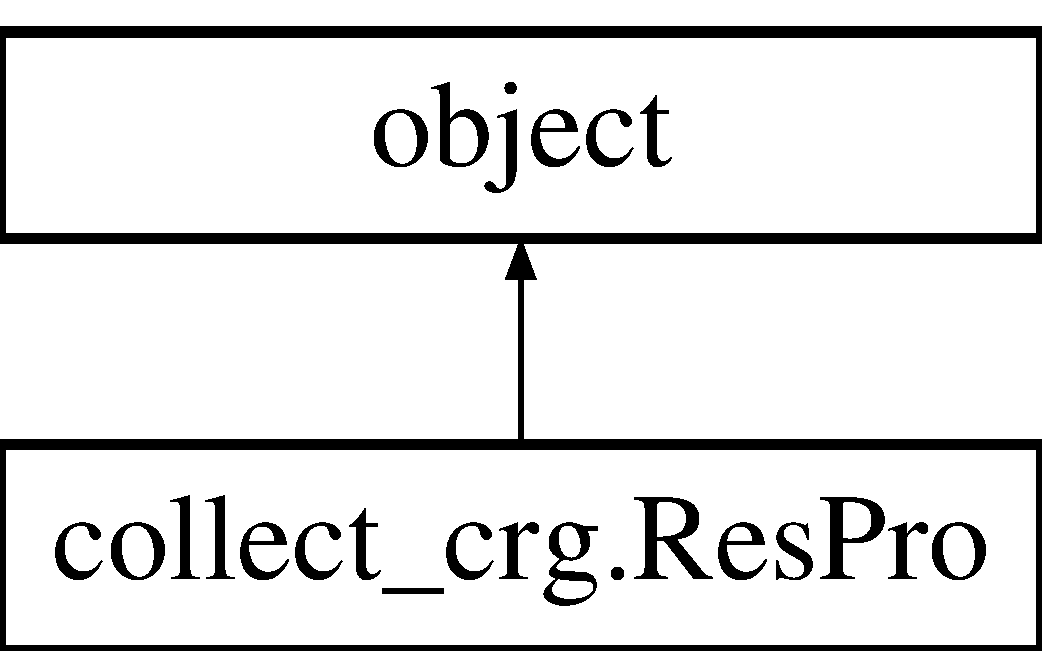
\includegraphics[height=2.000000cm]{classcollect__crg_1_1_res_pro}
\end{center}
\end{figure}
\subsection*{Public Member Functions}
\begin{DoxyCompactItemize}
\item 
def \hyperlink{classcollect__crg_1_1_res_pro_ab563227610708f8c5867c766b3b7d3e9}{\-\_\-\-\_\-init\-\_\-\-\_\-}
\item 
def \hyperlink{classcollect__crg_1_1_res_pro_ac4141791c8bd45b3ffe8b5ec2483bfc1}{\-\_\-\-\_\-str\-\_\-\-\_\-}
\end{DoxyCompactItemize}
\subsection*{Public Attributes}
\begin{DoxyCompactItemize}
\item 
\hyperlink{classcollect__crg_1_1_res_pro_a7075290e45b0608bb59ebfe42722b4e3}{charges}
\item 
\hyperlink{classcollect__crg_1_1_res_pro_aec2b2fecfffa4aa7728013ee504d48f7}{r\-Name}
\end{DoxyCompactItemize}
\subsection*{Static Public Attributes}
\begin{DoxyCompactItemize}
\item 
tuple \hyperlink{classcollect__crg_1_1_res_pro_a0978c5440914518afa5bba719a40bfa1}{all\-Run\-Types} = (\char`\"{}cqr\char`\"{}, \char`\"{}cql\char`\"{}, \char`\"{}cdr\char`\"{}, \char`\"{}cdl\char`\"{}, \char`\"{}hqr\char`\"{}, \char`\"{}hql\char`\"{}, \char`\"{}hdr\char`\"{}, \char`\"{}hdl\char`\"{})
\end{DoxyCompactItemize}
\subsection*{Static Private Attributes}
\begin{DoxyCompactItemize}
\item 
\hyperlink{classcollect__crg_1_1_res_pro_ab775338960aae2ea56892e7a39a6e63c}{\-\_\-\-\_\-repr\-\_\-\-\_\-} = \hyperlink{classcollect__crg_1_1_res_pro_ac4141791c8bd45b3ffe8b5ec2483bfc1}{\-\_\-\-\_\-str\-\_\-\-\_\-}
\end{DoxyCompactItemize}


\subsection{Detailed Description}
Residue class. 

It only contains the charges of the residues in different types of runs. 

\subsection{Constructor \& Destructor Documentation}
\hypertarget{classcollect__crg_1_1_res_pro_ab563227610708f8c5867c766b3b7d3e9}{\index{collect\-\_\-crg\-::\-Res\-Pro@{collect\-\_\-crg\-::\-Res\-Pro}!\-\_\-\-\_\-init\-\_\-\-\_\-@{\-\_\-\-\_\-init\-\_\-\-\_\-}}
\index{\-\_\-\-\_\-init\-\_\-\-\_\-@{\-\_\-\-\_\-init\-\_\-\-\_\-}!collect_crg::ResPro@{collect\-\_\-crg\-::\-Res\-Pro}}
\subsubsection[{\-\_\-\-\_\-init\-\_\-\-\_\-}]{\setlength{\rightskip}{0pt plus 5cm}def collect\-\_\-crg.\-Res\-Pro.\-\_\-\-\_\-init\-\_\-\-\_\- (
\begin{DoxyParamCaption}
\item[{}]{self, }
\item[{}]{name = {\ttfamily ''}}
\end{DoxyParamCaption}
)}}\label{classcollect__crg_1_1_res_pro_ab563227610708f8c5867c766b3b7d3e9}


\subsection{Member Function Documentation}
\hypertarget{classcollect__crg_1_1_res_pro_ac4141791c8bd45b3ffe8b5ec2483bfc1}{\index{collect\-\_\-crg\-::\-Res\-Pro@{collect\-\_\-crg\-::\-Res\-Pro}!\-\_\-\-\_\-str\-\_\-\-\_\-@{\-\_\-\-\_\-str\-\_\-\-\_\-}}
\index{\-\_\-\-\_\-str\-\_\-\-\_\-@{\-\_\-\-\_\-str\-\_\-\-\_\-}!collect_crg::ResPro@{collect\-\_\-crg\-::\-Res\-Pro}}
\subsubsection[{\-\_\-\-\_\-str\-\_\-\-\_\-}]{\setlength{\rightskip}{0pt plus 5cm}def collect\-\_\-crg.\-Res\-Pro.\-\_\-\-\_\-str\-\_\-\-\_\- (
\begin{DoxyParamCaption}
\item[{}]{self}
\end{DoxyParamCaption}
)}}\label{classcollect__crg_1_1_res_pro_ac4141791c8bd45b3ffe8b5ec2483bfc1}


\subsection{Member Data Documentation}
\hypertarget{classcollect__crg_1_1_res_pro_ab775338960aae2ea56892e7a39a6e63c}{\index{collect\-\_\-crg\-::\-Res\-Pro@{collect\-\_\-crg\-::\-Res\-Pro}!\-\_\-\-\_\-repr\-\_\-\-\_\-@{\-\_\-\-\_\-repr\-\_\-\-\_\-}}
\index{\-\_\-\-\_\-repr\-\_\-\-\_\-@{\-\_\-\-\_\-repr\-\_\-\-\_\-}!collect_crg::ResPro@{collect\-\_\-crg\-::\-Res\-Pro}}
\subsubsection[{\-\_\-\-\_\-repr\-\_\-\-\_\-}]{\setlength{\rightskip}{0pt plus 5cm}collect\-\_\-crg.\-Res\-Pro.\-\_\-\-\_\-repr\-\_\-\-\_\- = {\bf \-\_\-\-\_\-str\-\_\-\-\_\-}\hspace{0.3cm}{\ttfamily [static]}, {\ttfamily [private]}}}\label{classcollect__crg_1_1_res_pro_ab775338960aae2ea56892e7a39a6e63c}
\hypertarget{classcollect__crg_1_1_res_pro_a0978c5440914518afa5bba719a40bfa1}{\index{collect\-\_\-crg\-::\-Res\-Pro@{collect\-\_\-crg\-::\-Res\-Pro}!all\-Run\-Types@{all\-Run\-Types}}
\index{all\-Run\-Types@{all\-Run\-Types}!collect_crg::ResPro@{collect\-\_\-crg\-::\-Res\-Pro}}
\subsubsection[{all\-Run\-Types}]{\setlength{\rightskip}{0pt plus 5cm}tuple collect\-\_\-crg.\-Res\-Pro.\-all\-Run\-Types = (\char`\"{}cqr\char`\"{}, \char`\"{}cql\char`\"{}, \char`\"{}cdr\char`\"{}, \char`\"{}cdl\char`\"{}, \char`\"{}hqr\char`\"{}, \char`\"{}hql\char`\"{}, \char`\"{}hdr\char`\"{}, \char`\"{}hdl\char`\"{})\hspace{0.3cm}{\ttfamily [static]}}}\label{classcollect__crg_1_1_res_pro_a0978c5440914518afa5bba719a40bfa1}
\hypertarget{classcollect__crg_1_1_res_pro_a7075290e45b0608bb59ebfe42722b4e3}{\index{collect\-\_\-crg\-::\-Res\-Pro@{collect\-\_\-crg\-::\-Res\-Pro}!charges@{charges}}
\index{charges@{charges}!collect_crg::ResPro@{collect\-\_\-crg\-::\-Res\-Pro}}
\subsubsection[{charges}]{\setlength{\rightskip}{0pt plus 5cm}collect\-\_\-crg.\-Res\-Pro.\-charges}}\label{classcollect__crg_1_1_res_pro_a7075290e45b0608bb59ebfe42722b4e3}
\hypertarget{classcollect__crg_1_1_res_pro_aec2b2fecfffa4aa7728013ee504d48f7}{\index{collect\-\_\-crg\-::\-Res\-Pro@{collect\-\_\-crg\-::\-Res\-Pro}!r\-Name@{r\-Name}}
\index{r\-Name@{r\-Name}!collect_crg::ResPro@{collect\-\_\-crg\-::\-Res\-Pro}}
\subsubsection[{r\-Name}]{\setlength{\rightskip}{0pt plus 5cm}collect\-\_\-crg.\-Res\-Pro.\-r\-Name}}\label{classcollect__crg_1_1_res_pro_aec2b2fecfffa4aa7728013ee504d48f7}


The documentation for this class was generated from the following file\-:\begin{DoxyCompactItemize}
\item 
src/scripts/mcce/\hyperlink{collect__crg_8py}{collect\-\_\-crg.\-py}\end{DoxyCompactItemize}

\hypertarget{classsetuptest_1_1_testrun}{\section{setuptest.\-Testrun Class Reference}
\label{classsetuptest_1_1_testrun}\index{setuptest.\-Testrun@{setuptest.\-Testrun}}
}
Inheritance diagram for setuptest.\-Testrun\-:\begin{figure}[H]
\begin{center}
\leavevmode
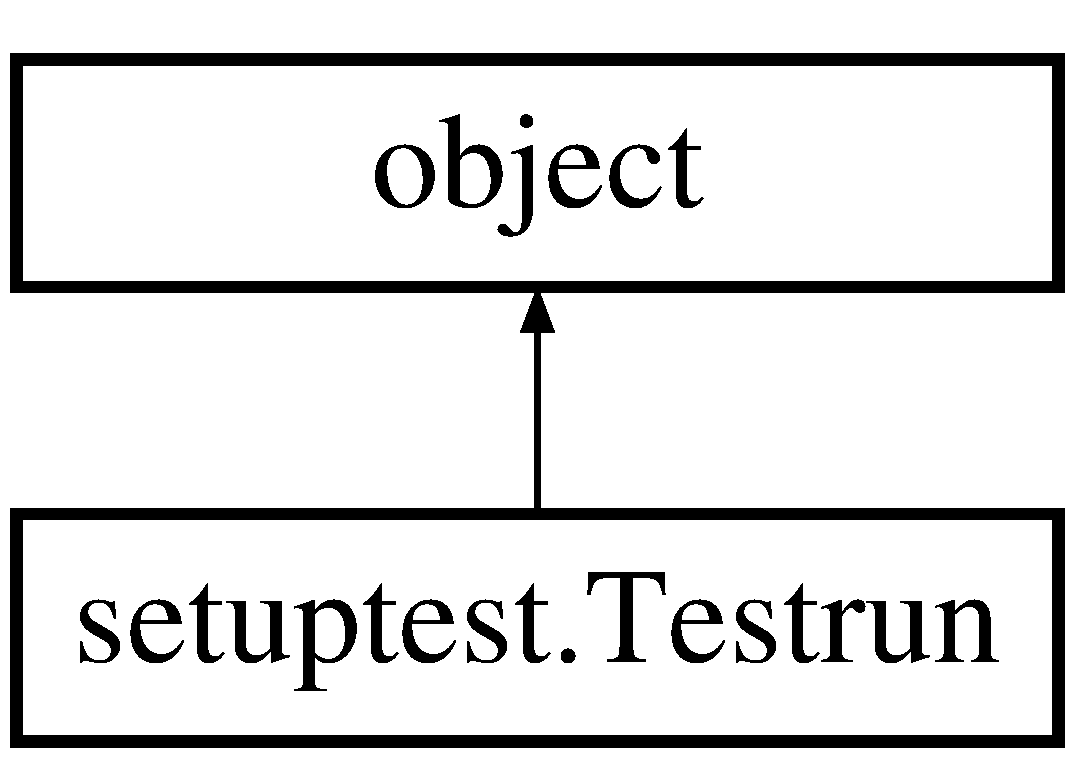
\includegraphics[height=2.000000cm]{classsetuptest_1_1_testrun}
\end{center}
\end{figure}
\subsection*{Public Member Functions}
\begin{DoxyCompactItemize}
\item 
def \hyperlink{classsetuptest_1_1_testrun_ababce1d63182e8b77fe6b6bf393cb656}{\-\_\-\-\_\-init\-\_\-\-\_\-}
\item 
def \hyperlink{classsetuptest_1_1_testrun_a0748a698b86bc66fc296b3708c5f856c}{submit\-Run}
\item 
def \hyperlink{classsetuptest_1_1_testrun_a4f355a4e1ca30600e384ef21e9b4f19a}{read\-\_\-mc\-\_\-out}
\item 
def \hyperlink{classsetuptest_1_1_testrun_a63f11436b0d8dc23cbcce8a216b0e8e1}{is\-Finished}
\begin{DoxyCompactList}\small\item\em Check whether this run is finished. \end{DoxyCompactList}\end{DoxyCompactItemize}
\subsection*{Public Attributes}
\begin{DoxyCompactItemize}
\item 
\hyperlink{classsetuptest_1_1_testrun_af05acc8d16596926b99889d80bc1d5a2}{annealing}
\item 
\hyperlink{classsetuptest_1_1_testrun_a75d610694fb72c84c3fd8b32b82a748c}{equilibration}
\item 
\hyperlink{classsetuptest_1_1_testrun_aabb9f14dd901cdceeb0f0884341ff8c5}{sampling}
\item 
\hyperlink{classsetuptest_1_1_testrun_a82322256ed240db2a584a35134b3e43b}{indep}
\item 
\hyperlink{classsetuptest_1_1_testrun_afc9309e5536064a4cf772c9345e39fbd}{name}
\item 
\hyperlink{classsetuptest_1_1_testrun_acc3824b952287ea8ae5be81cff73a0dc}{avg\-Energies}
\item 
\hyperlink{classsetuptest_1_1_testrun_a83eda4a8be5751c070ccff7ae9ba5b8f}{all\-M\-C\-Energies}
\item 
\hyperlink{classsetuptest_1_1_testrun_a1420fdcf878658bf1bc6e19ffb30a572}{mc\-Samplings}
\item 
\hyperlink{classsetuptest_1_1_testrun_ab21fecaca25ab0cdf2a378eceecc08ab}{conformers}
\item 
\hyperlink{classsetuptest_1_1_testrun_a0c18cf42e638472b96e8884474d97045}{largeststd}
\end{DoxyCompactItemize}


\subsection{Constructor \& Destructor Documentation}
\hypertarget{classsetuptest_1_1_testrun_ababce1d63182e8b77fe6b6bf393cb656}{\index{setuptest\-::\-Testrun@{setuptest\-::\-Testrun}!\-\_\-\-\_\-init\-\_\-\-\_\-@{\-\_\-\-\_\-init\-\_\-\-\_\-}}
\index{\-\_\-\-\_\-init\-\_\-\-\_\-@{\-\_\-\-\_\-init\-\_\-\-\_\-}!setuptest::Testrun@{setuptest\-::\-Testrun}}
\subsubsection[{\-\_\-\-\_\-init\-\_\-\-\_\-}]{\setlength{\rightskip}{0pt plus 5cm}def setuptest.\-Testrun.\-\_\-\-\_\-init\-\_\-\-\_\- (
\begin{DoxyParamCaption}
\item[{}]{self, }
\item[{}]{name, }
\item[{}]{a = {\ttfamily 100}, }
\item[{}]{e = {\ttfamily 300}, }
\item[{}]{s = {\ttfamily 2000}, }
\item[{}]{i = {\ttfamily 6}}
\end{DoxyParamCaption}
)}}\label{classsetuptest_1_1_testrun_ababce1d63182e8b77fe6b6bf393cb656}


\subsection{Member Function Documentation}
\hypertarget{classsetuptest_1_1_testrun_a63f11436b0d8dc23cbcce8a216b0e8e1}{\index{setuptest\-::\-Testrun@{setuptest\-::\-Testrun}!is\-Finished@{is\-Finished}}
\index{is\-Finished@{is\-Finished}!setuptest::Testrun@{setuptest\-::\-Testrun}}
\subsubsection[{is\-Finished}]{\setlength{\rightskip}{0pt plus 5cm}def setuptest.\-Testrun.\-is\-Finished (
\begin{DoxyParamCaption}
\item[{}]{self, }
\item[{}]{work\-Path}
\end{DoxyParamCaption}
)}}\label{classsetuptest_1_1_testrun_a63f11436b0d8dc23cbcce8a216b0e8e1}


Check whether this run is finished. 

\hypertarget{classsetuptest_1_1_testrun_a4f355a4e1ca30600e384ef21e9b4f19a}{\index{setuptest\-::\-Testrun@{setuptest\-::\-Testrun}!read\-\_\-mc\-\_\-out@{read\-\_\-mc\-\_\-out}}
\index{read\-\_\-mc\-\_\-out@{read\-\_\-mc\-\_\-out}!setuptest::Testrun@{setuptest\-::\-Testrun}}
\subsubsection[{read\-\_\-mc\-\_\-out}]{\setlength{\rightskip}{0pt plus 5cm}def setuptest.\-Testrun.\-read\-\_\-mc\-\_\-out (
\begin{DoxyParamCaption}
\item[{}]{self, }
\item[{}]{fname = {\ttfamily \char`\"{}mc\-\_\-out\char`\"{}}, }
\item[{}]{kwargv}
\end{DoxyParamCaption}
)}}\label{classsetuptest_1_1_testrun_a4f355a4e1ca30600e384ef21e9b4f19a}
\hypertarget{classsetuptest_1_1_testrun_a0748a698b86bc66fc296b3708c5f856c}{\index{setuptest\-::\-Testrun@{setuptest\-::\-Testrun}!submit\-Run@{submit\-Run}}
\index{submit\-Run@{submit\-Run}!setuptest::Testrun@{setuptest\-::\-Testrun}}
\subsubsection[{submit\-Run}]{\setlength{\rightskip}{0pt plus 5cm}def setuptest.\-Testrun.\-submit\-Run (
\begin{DoxyParamCaption}
\item[{}]{self, }
\item[{}]{parent\-Path}
\end{DoxyParamCaption}
)}}\label{classsetuptest_1_1_testrun_a0748a698b86bc66fc296b3708c5f856c}


\subsection{Member Data Documentation}
\hypertarget{classsetuptest_1_1_testrun_a83eda4a8be5751c070ccff7ae9ba5b8f}{\index{setuptest\-::\-Testrun@{setuptest\-::\-Testrun}!all\-M\-C\-Energies@{all\-M\-C\-Energies}}
\index{all\-M\-C\-Energies@{all\-M\-C\-Energies}!setuptest::Testrun@{setuptest\-::\-Testrun}}
\subsubsection[{all\-M\-C\-Energies}]{\setlength{\rightskip}{0pt plus 5cm}setuptest.\-Testrun.\-all\-M\-C\-Energies}}\label{classsetuptest_1_1_testrun_a83eda4a8be5751c070ccff7ae9ba5b8f}
\hypertarget{classsetuptest_1_1_testrun_af05acc8d16596926b99889d80bc1d5a2}{\index{setuptest\-::\-Testrun@{setuptest\-::\-Testrun}!annealing@{annealing}}
\index{annealing@{annealing}!setuptest::Testrun@{setuptest\-::\-Testrun}}
\subsubsection[{annealing}]{\setlength{\rightskip}{0pt plus 5cm}setuptest.\-Testrun.\-annealing}}\label{classsetuptest_1_1_testrun_af05acc8d16596926b99889d80bc1d5a2}
\hypertarget{classsetuptest_1_1_testrun_acc3824b952287ea8ae5be81cff73a0dc}{\index{setuptest\-::\-Testrun@{setuptest\-::\-Testrun}!avg\-Energies@{avg\-Energies}}
\index{avg\-Energies@{avg\-Energies}!setuptest::Testrun@{setuptest\-::\-Testrun}}
\subsubsection[{avg\-Energies}]{\setlength{\rightskip}{0pt plus 5cm}setuptest.\-Testrun.\-avg\-Energies}}\label{classsetuptest_1_1_testrun_acc3824b952287ea8ae5be81cff73a0dc}
\hypertarget{classsetuptest_1_1_testrun_ab21fecaca25ab0cdf2a378eceecc08ab}{\index{setuptest\-::\-Testrun@{setuptest\-::\-Testrun}!conformers@{conformers}}
\index{conformers@{conformers}!setuptest::Testrun@{setuptest\-::\-Testrun}}
\subsubsection[{conformers}]{\setlength{\rightskip}{0pt plus 5cm}setuptest.\-Testrun.\-conformers}}\label{classsetuptest_1_1_testrun_ab21fecaca25ab0cdf2a378eceecc08ab}
\hypertarget{classsetuptest_1_1_testrun_a75d610694fb72c84c3fd8b32b82a748c}{\index{setuptest\-::\-Testrun@{setuptest\-::\-Testrun}!equilibration@{equilibration}}
\index{equilibration@{equilibration}!setuptest::Testrun@{setuptest\-::\-Testrun}}
\subsubsection[{equilibration}]{\setlength{\rightskip}{0pt plus 5cm}setuptest.\-Testrun.\-equilibration}}\label{classsetuptest_1_1_testrun_a75d610694fb72c84c3fd8b32b82a748c}
\hypertarget{classsetuptest_1_1_testrun_a82322256ed240db2a584a35134b3e43b}{\index{setuptest\-::\-Testrun@{setuptest\-::\-Testrun}!indep@{indep}}
\index{indep@{indep}!setuptest::Testrun@{setuptest\-::\-Testrun}}
\subsubsection[{indep}]{\setlength{\rightskip}{0pt plus 5cm}setuptest.\-Testrun.\-indep}}\label{classsetuptest_1_1_testrun_a82322256ed240db2a584a35134b3e43b}
\hypertarget{classsetuptest_1_1_testrun_a0c18cf42e638472b96e8884474d97045}{\index{setuptest\-::\-Testrun@{setuptest\-::\-Testrun}!largeststd@{largeststd}}
\index{largeststd@{largeststd}!setuptest::Testrun@{setuptest\-::\-Testrun}}
\subsubsection[{largeststd}]{\setlength{\rightskip}{0pt plus 5cm}setuptest.\-Testrun.\-largeststd}}\label{classsetuptest_1_1_testrun_a0c18cf42e638472b96e8884474d97045}
\hypertarget{classsetuptest_1_1_testrun_a1420fdcf878658bf1bc6e19ffb30a572}{\index{setuptest\-::\-Testrun@{setuptest\-::\-Testrun}!mc\-Samplings@{mc\-Samplings}}
\index{mc\-Samplings@{mc\-Samplings}!setuptest::Testrun@{setuptest\-::\-Testrun}}
\subsubsection[{mc\-Samplings}]{\setlength{\rightskip}{0pt plus 5cm}setuptest.\-Testrun.\-mc\-Samplings}}\label{classsetuptest_1_1_testrun_a1420fdcf878658bf1bc6e19ffb30a572}
\hypertarget{classsetuptest_1_1_testrun_afc9309e5536064a4cf772c9345e39fbd}{\index{setuptest\-::\-Testrun@{setuptest\-::\-Testrun}!name@{name}}
\index{name@{name}!setuptest::Testrun@{setuptest\-::\-Testrun}}
\subsubsection[{name}]{\setlength{\rightskip}{0pt plus 5cm}setuptest.\-Testrun.\-name}}\label{classsetuptest_1_1_testrun_afc9309e5536064a4cf772c9345e39fbd}
\hypertarget{classsetuptest_1_1_testrun_aabb9f14dd901cdceeb0f0884341ff8c5}{\index{setuptest\-::\-Testrun@{setuptest\-::\-Testrun}!sampling@{sampling}}
\index{sampling@{sampling}!setuptest::Testrun@{setuptest\-::\-Testrun}}
\subsubsection[{sampling}]{\setlength{\rightskip}{0pt plus 5cm}setuptest.\-Testrun.\-sampling}}\label{classsetuptest_1_1_testrun_aabb9f14dd901cdceeb0f0884341ff8c5}


The documentation for this class was generated from the following file\-:\begin{DoxyCompactItemize}
\item 
src/scripts/old/\hyperlink{setuptest_8py}{setuptest.\-py}\end{DoxyCompactItemize}

\hypertarget{classwater__stat_1_1_wat}{\section{water\-\_\-stat.\-Wat Class Reference}
\label{classwater__stat_1_1_wat}\index{water\-\_\-stat.\-Wat@{water\-\_\-stat.\-Wat}}
}


Water class.  


Inheritance diagram for water\-\_\-stat.\-Wat\-:\begin{figure}[H]
\begin{center}
\leavevmode
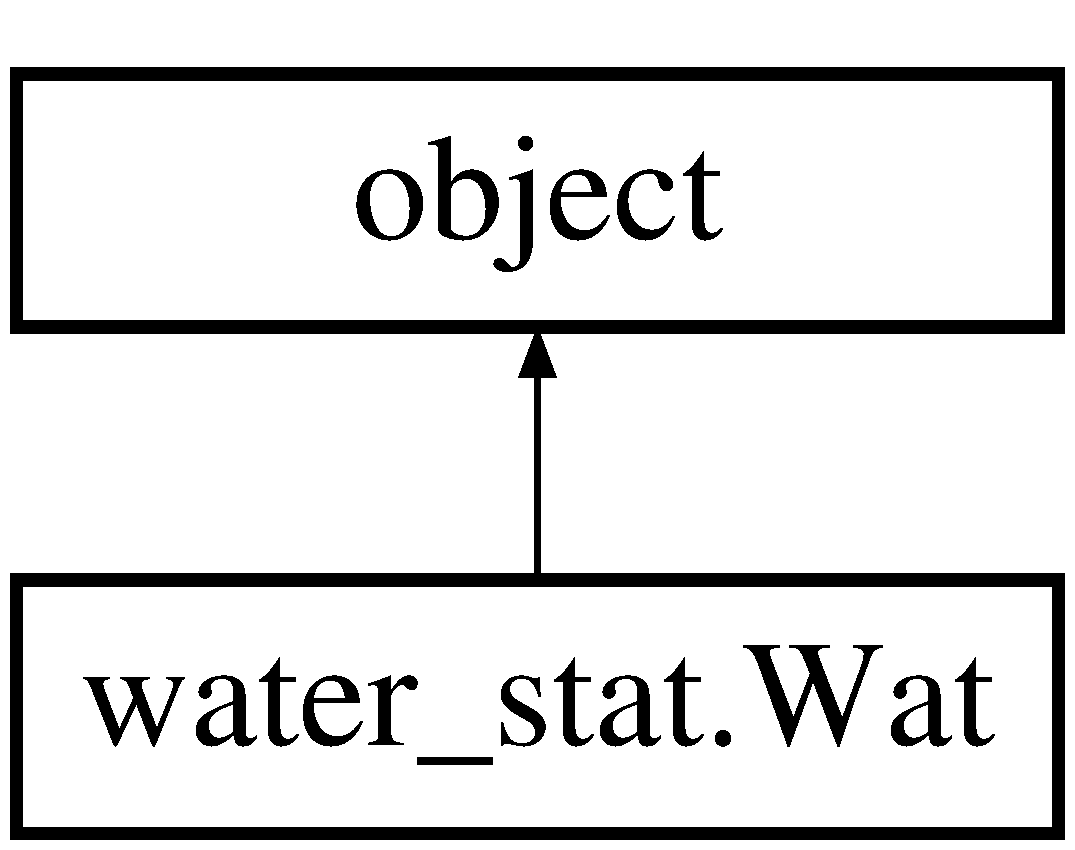
\includegraphics[height=2.000000cm]{classwater__stat_1_1_wat}
\end{center}
\end{figure}
\subsection*{Public Member Functions}
\begin{DoxyCompactItemize}
\item 
def \hyperlink{classwater__stat_1_1_wat_a6b772a3834cf4c0aa0b7a299fcd54bd6}{\-\_\-\-\_\-init\-\_\-\-\_\-}
\begin{DoxyCompactList}\small\item\em Initialization. \end{DoxyCompactList}\end{DoxyCompactItemize}
\subsection*{Public Attributes}
\begin{DoxyCompactItemize}
\item 
\hyperlink{classwater__stat_1_1_wat_a09896d64e2686c9933dfdb9f7d1c6ac4}{res\-Name}
\item 
\hyperlink{classwater__stat_1_1_wat_a72e4fb0d4a84ae25854d58570dc2dbbe}{dummy\-Occ}
\end{DoxyCompactItemize}


\subsection{Detailed Description}
Water class. 

\subsection{Constructor \& Destructor Documentation}
\hypertarget{classwater__stat_1_1_wat_a6b772a3834cf4c0aa0b7a299fcd54bd6}{\index{water\-\_\-stat\-::\-Wat@{water\-\_\-stat\-::\-Wat}!\-\_\-\-\_\-init\-\_\-\-\_\-@{\-\_\-\-\_\-init\-\_\-\-\_\-}}
\index{\-\_\-\-\_\-init\-\_\-\-\_\-@{\-\_\-\-\_\-init\-\_\-\-\_\-}!water_stat::Wat@{water\-\_\-stat\-::\-Wat}}
\subsubsection[{\-\_\-\-\_\-init\-\_\-\-\_\-}]{\setlength{\rightskip}{0pt plus 5cm}def water\-\_\-stat.\-Wat.\-\_\-\-\_\-init\-\_\-\-\_\- (
\begin{DoxyParamCaption}
\item[{}]{self, }
\item[{}]{res\-Name = {\ttfamily \char`\"{}\char`\"{}}, }
\item[{}]{occ = {\ttfamily 0.0}}
\end{DoxyParamCaption}
)}}\label{classwater__stat_1_1_wat_a6b772a3834cf4c0aa0b7a299fcd54bd6}


Initialization. 

Args\-: res\-Name (str)\-: name of the residue (water), like H\-O\-H\-A0403. occ (float, optional)\-: occupancy of the dummy conformer of the water. 

\subsection{Member Data Documentation}
\hypertarget{classwater__stat_1_1_wat_a72e4fb0d4a84ae25854d58570dc2dbbe}{\index{water\-\_\-stat\-::\-Wat@{water\-\_\-stat\-::\-Wat}!dummy\-Occ@{dummy\-Occ}}
\index{dummy\-Occ@{dummy\-Occ}!water_stat::Wat@{water\-\_\-stat\-::\-Wat}}
\subsubsection[{dummy\-Occ}]{\setlength{\rightskip}{0pt plus 5cm}water\-\_\-stat.\-Wat.\-dummy\-Occ}}\label{classwater__stat_1_1_wat_a72e4fb0d4a84ae25854d58570dc2dbbe}
\hypertarget{classwater__stat_1_1_wat_a09896d64e2686c9933dfdb9f7d1c6ac4}{\index{water\-\_\-stat\-::\-Wat@{water\-\_\-stat\-::\-Wat}!res\-Name@{res\-Name}}
\index{res\-Name@{res\-Name}!water_stat::Wat@{water\-\_\-stat\-::\-Wat}}
\subsubsection[{res\-Name}]{\setlength{\rightskip}{0pt plus 5cm}water\-\_\-stat.\-Wat.\-res\-Name}}\label{classwater__stat_1_1_wat_a09896d64e2686c9933dfdb9f7d1c6ac4}


The documentation for this class was generated from the following file\-:\begin{DoxyCompactItemize}
\item 
src/scripts/old/\hyperlink{water__stat_8py}{water\-\_\-stat.\-py}\end{DoxyCompactItemize}

\hypertarget{classcomp__desol_1_1_water_conf}{\section{comp\-\_\-desol.\-Water\-Conf Class Reference}
\label{classcomp__desol_1_1_water_conf}\index{comp\-\_\-desol.\-Water\-Conf@{comp\-\_\-desol.\-Water\-Conf}}
}


Compare the desolvation energies of waters.  


Inheritance diagram for comp\-\_\-desol.\-Water\-Conf\-:\begin{figure}[H]
\begin{center}
\leavevmode
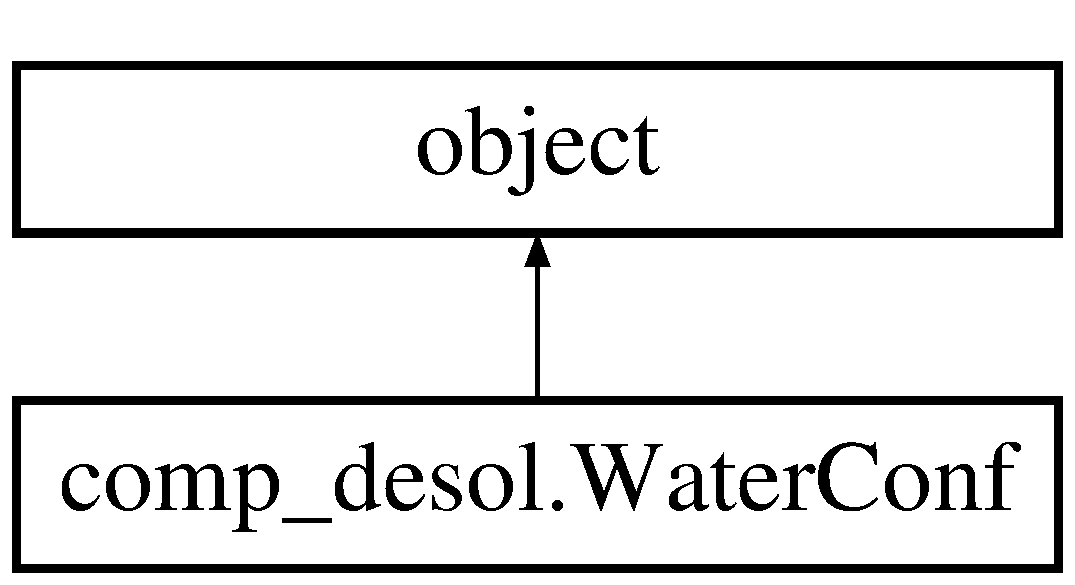
\includegraphics[height=2.000000cm]{classcomp__desol_1_1_water_conf}
\end{center}
\end{figure}
\subsection*{Public Member Functions}
\begin{DoxyCompactItemize}
\item 
def \hyperlink{classcomp__desol_1_1_water_conf_a0fb421de7d4a112769e5da6004c51b93}{\-\_\-\-\_\-init\-\_\-\-\_\-}
\end{DoxyCompactItemize}
\subsection*{Public Attributes}
\begin{DoxyCompactItemize}
\item 
\hyperlink{classcomp__desol_1_1_water_conf_a5b1921836f354b358be05d4ea6b93ae6}{conf\-Name}
\item 
\hyperlink{classcomp__desol_1_1_water_conf_aaf4a467d6793dea2e163ba5e7aa1888c}{desolv}
\end{DoxyCompactItemize}


\subsection{Detailed Description}
Compare the desolvation energies of waters. 

Water conformer class. 

\subsection{Constructor \& Destructor Documentation}
\hypertarget{classcomp__desol_1_1_water_conf_a0fb421de7d4a112769e5da6004c51b93}{\index{comp\-\_\-desol\-::\-Water\-Conf@{comp\-\_\-desol\-::\-Water\-Conf}!\-\_\-\-\_\-init\-\_\-\-\_\-@{\-\_\-\-\_\-init\-\_\-\-\_\-}}
\index{\-\_\-\-\_\-init\-\_\-\-\_\-@{\-\_\-\-\_\-init\-\_\-\-\_\-}!comp_desol::WaterConf@{comp\-\_\-desol\-::\-Water\-Conf}}
\subsubsection[{\-\_\-\-\_\-init\-\_\-\-\_\-}]{\setlength{\rightskip}{0pt plus 5cm}def comp\-\_\-desol.\-Water\-Conf.\-\_\-\-\_\-init\-\_\-\-\_\- (
\begin{DoxyParamCaption}
\item[{}]{self}
\end{DoxyParamCaption}
)}}\label{classcomp__desol_1_1_water_conf_a0fb421de7d4a112769e5da6004c51b93}


\subsection{Member Data Documentation}
\hypertarget{classcomp__desol_1_1_water_conf_a5b1921836f354b358be05d4ea6b93ae6}{\index{comp\-\_\-desol\-::\-Water\-Conf@{comp\-\_\-desol\-::\-Water\-Conf}!conf\-Name@{conf\-Name}}
\index{conf\-Name@{conf\-Name}!comp_desol::WaterConf@{comp\-\_\-desol\-::\-Water\-Conf}}
\subsubsection[{conf\-Name}]{\setlength{\rightskip}{0pt plus 5cm}comp\-\_\-desol.\-Water\-Conf.\-conf\-Name}}\label{classcomp__desol_1_1_water_conf_a5b1921836f354b358be05d4ea6b93ae6}
\hypertarget{classcomp__desol_1_1_water_conf_aaf4a467d6793dea2e163ba5e7aa1888c}{\index{comp\-\_\-desol\-::\-Water\-Conf@{comp\-\_\-desol\-::\-Water\-Conf}!desolv@{desolv}}
\index{desolv@{desolv}!comp_desol::WaterConf@{comp\-\_\-desol\-::\-Water\-Conf}}
\subsubsection[{desolv}]{\setlength{\rightskip}{0pt plus 5cm}comp\-\_\-desol.\-Water\-Conf.\-desolv}}\label{classcomp__desol_1_1_water_conf_aaf4a467d6793dea2e163ba5e7aa1888c}


The documentation for this class was generated from the following file\-:\begin{DoxyCompactItemize}
\item 
src/scripts/mcce/\hyperlink{comp__desol_8py}{comp\-\_\-desol.\-py}\end{DoxyCompactItemize}

\chapter{File Documentation}
\hypertarget{analyze_network_8py}{\section{src/scripts/hb\-\_\-connection/analyze\-Network.py File Reference}
\label{analyze_network_8py}\index{src/scripts/hb\-\_\-connection/analyze\-Network.\-py@{src/scripts/hb\-\_\-connection/analyze\-Network.\-py}}
}
\subsection*{Namespaces}
\begin{DoxyCompactItemize}
\item 
\hyperlink{namespaceanalyze_network}{analyze\-Network}
\end{DoxyCompactItemize}
\subsection*{Functions}
\begin{DoxyCompactItemize}
\item 
def \hyperlink{namespaceanalyze_network_a35ddd1b09f75100c977b787de09e9a98}{analyze\-Network.\-main}
\item 
def \hyperlink{namespaceanalyze_network_a23533653f6b89a1dc1e54b1dfda919af}{analyze\-Network.\-make\-Path\-Info\-File}
\item 
def \hyperlink{namespaceanalyze_network_a1d771169ef3f40af2da197fce52333b5}{analyze\-Network.\-load\-Res\-Protonation}
\end{DoxyCompactItemize}
\subsection*{Variables}
\begin{DoxyCompactItemize}
\item 
int \hyperlink{namespaceanalyze_network_a9522a4ca48f20aa3cc2230c0d094f49f}{analyze\-Network.\-D\-U\-M\-M\-Y\-\_\-\-P\-R\-O\-T\-O\-N\-A\-T\-I\-O\-N} = 211
\item 
dictionary \hyperlink{namespaceanalyze_network_a4af941f8433e14aa7d958e74cc6272b8}{analyze\-Network.\-P\-O\-S\-S\-I\-B\-L\-E\-\_\-\-P\-R\-O\-T\-O\-N\-A\-T\-I\-O\-N\-S}
\end{DoxyCompactItemize}

\hypertarget{arg82__conn_8py}{\section{src/scripts/hb\-\_\-connection/arg82\-\_\-conn.py File Reference}
\label{arg82__conn_8py}\index{src/scripts/hb\-\_\-connection/arg82\-\_\-conn.\-py@{src/scripts/hb\-\_\-connection/arg82\-\_\-conn.\-py}}
}
\subsection*{Classes}
\begin{DoxyCompactItemize}
\item 
class \hyperlink{classarg82__conn_1_1_protonation_state}{arg82\-\_\-conn.\-Protonation\-State}
\item 
class \hyperlink{classarg82__conn_1_1_hop_sequence}{arg82\-\_\-conn.\-Hop\-Sequence}
\item 
class \hyperlink{classarg82__conn_1_1_hb_path}{arg82\-\_\-conn.\-Hb\-Path}
\item 
class \hyperlink{classarg82__conn_1_1_conf}{arg82\-\_\-conn.\-Conf}
\end{DoxyCompactItemize}
\subsection*{Namespaces}
\begin{DoxyCompactItemize}
\item 
\hyperlink{namespacearg82__conn}{arg82\-\_\-conn}
\end{DoxyCompactItemize}
\subsection*{Functions}
\begin{DoxyCompactItemize}
\item 
def \hyperlink{namespacearg82__conn_a0e915959a01aeb1a5af59191966b9ac8}{arg82\-\_\-conn.\-occonf}
\item 
def \hyperlink{namespacearg82__conn_af60ebd9bfc139eee093b86579bc02e3a}{arg82\-\_\-conn.\-most\-\_\-occ\-\_\-conf}
\item 
def \hyperlink{namespacearg82__conn_aa2a85f84b25b079994c07aae005513f5}{arg82\-\_\-conn.\-occupied\-\_\-arg}
\item 
def \hyperlink{namespacearg82__conn_a654bc7307bad1f2c60c8d9c8b946f07f}{arg82\-\_\-conn.\-main}
\end{DoxyCompactItemize}
\subsection*{Variables}
\begin{DoxyCompactItemize}
\item 
string \hyperlink{namespacearg82__conn_a1118fc69bf72cf5c0c6af8860ac1ac98}{arg82\-\_\-conn.\-S\-U\-B\-\_\-\-R\-U\-N\-S\-\_\-\-F\-O\-L\-D\-E\-R} = \char`\"{}m\-Sub\char`\"{}
\item 
string \hyperlink{namespacearg82__conn_ad6e38f362ded631c94bea165ee760673}{arg82\-\_\-conn.\-P\-A\-T\-H\-\_\-\-I\-N\-F\-O\-\_\-\-F\-I\-L\-E} = \char`\"{}pathinfo.\-txt\char`\"{}
\item 
int \hyperlink{namespacearg82__conn_a7f9b0ba0df45cb729820b40149d23b2d}{arg82\-\_\-conn.\-D\-U\-M\-M\-Y\-\_\-\-P\-R\-O\-T\-O\-N\-A\-T\-I\-O\-N} = 211
\item 
dictionary \hyperlink{namespacearg82__conn_ac3320beedaddd48f95e875b543d3a177}{arg82\-\_\-conn.\-C\-O\-N\-V\-E\-R\-T\-\_\-\-R\-E\-S\-\_\-\-S\-Y\-M\-B\-O\-L} = \{\char`\"{}A\-S\-P\char`\"{}\-:'D', \char`\"{}G\-L\-U\char`\"{}\-:'E', \char`\"{}A\-R\-G\char`\"{}\-:'R', \char`\"{}H\-O\-H\char`\"{}\-:'O', \char`\"{}T\-Y\-R\char`\"{}\-:'Y', \char`\"{}R\-S\-B\char`\"{}\-:'U'\}
\item 
dictionary \hyperlink{namespacearg82__conn_ae79f5cbbaaddf7a4aa3fd0b6d46b2bd2}{arg82\-\_\-conn.\-C\-O\-N\-V\-E\-R\-T\-\_\-\-P\-R\-O\-T\-O\-N\-A\-T\-I\-O\-N\-\_\-\-S\-Y\-M\-B\-O\-L} = \{-\/1\-:'-\/', 0\-:'0', +1\-:'+'\}
\item 
dictionary \hyperlink{namespacearg82__conn_a34f2a20ec5c6b3f3e697fabc4d5fd6f4}{arg82\-\_\-conn.\-C\-O\-N\-V\-E\-R\-T\-\_\-\-S\-Y\-M\-B\-O\-L\-\_\-\-P\-R\-O\-T\-O\-N\-A\-T\-I\-O\-N} = \{'-\/'\-:-\/1, '0'\-:0, '+'\-:1\}
\end{DoxyCompactItemize}

\hypertarget{atom__hbond_8py}{\section{src/scripts/hb\-\_\-connection/atom\-\_\-hbond.py File Reference}
\label{atom__hbond_8py}\index{src/scripts/hb\-\_\-connection/atom\-\_\-hbond.\-py@{src/scripts/hb\-\_\-connection/atom\-\_\-hbond.\-py}}
}
\subsection*{Classes}
\begin{DoxyCompactItemize}
\item 
class \hyperlink{classatom__hbond_1_1_res_node}{atom\-\_\-hbond.\-Res\-Node}
\item 
class \hyperlink{classatom__hbond_1_1_res_edge}{atom\-\_\-hbond.\-Res\-Edge}
\item 
class \hyperlink{classatom__hbond_1_1_hbond}{atom\-\_\-hbond.\-Hbond}
\item 
class \hyperlink{classatom__hbond_1_1_atom_net}{atom\-\_\-hbond.\-Atom\-Net}
\end{DoxyCompactItemize}
\subsection*{Namespaces}
\begin{DoxyCompactItemize}
\item 
\hyperlink{namespaceatom__hbond}{atom\-\_\-hbond}
\end{DoxyCompactItemize}
\subsection*{Functions}
\begin{DoxyCompactItemize}
\item 
def \hyperlink{namespaceatom__hbond_ab98e87c51126e44e505a16d4d2d9f56e}{atom\-\_\-hbond.\-main}
\end{DoxyCompactItemize}

\hypertarget{atom__net_8py}{\section{src/scripts/hb\-\_\-connection/atom\-\_\-net.py File Reference}
\label{atom__net_8py}\index{src/scripts/hb\-\_\-connection/atom\-\_\-net.\-py@{src/scripts/hb\-\_\-connection/atom\-\_\-net.\-py}}
}
\subsection*{Namespaces}
\begin{DoxyCompactItemize}
\item 
\hyperlink{namespaceatom__net}{atom\-\_\-net}
\end{DoxyCompactItemize}

\hypertarget{hbnet_8py}{\section{src/scripts/hb\-\_\-connection/hbnet.py File Reference}
\label{hbnet_8py}\index{src/scripts/hb\-\_\-connection/hbnet.\-py@{src/scripts/hb\-\_\-connection/hbnet.\-py}}
}
\subsection*{Classes}
\begin{DoxyCompactItemize}
\item 
class \hyperlink{classhbnet_1_1_protonation_state}{hbnet.\-Protonation\-State}
\item 
class \hyperlink{classhbnet_1_1_hop_sequence}{hbnet.\-Hop\-Sequence}
\item 
class \hyperlink{classhbnet_1_1_hb_path}{hbnet.\-Hb\-Path}
\end{DoxyCompactItemize}
\subsection*{Namespaces}
\begin{DoxyCompactItemize}
\item 
\hyperlink{namespacehbnet}{hbnet}
\end{DoxyCompactItemize}
\subsection*{Variables}
\begin{DoxyCompactItemize}
\item 
string \hyperlink{namespacehbnet_add488ebbd46a3a78639e26cd87fdc2b7}{hbnet.\-S\-U\-B\-\_\-\-R\-U\-N\-S\-\_\-\-F\-O\-L\-D\-E\-R} = \char`\"{}m\-Sub\char`\"{}
\item 
string \hyperlink{namespacehbnet_aadb238781e56973ec548da8d15fb2ea2}{hbnet.\-P\-A\-T\-H\-\_\-\-I\-N\-F\-O\-\_\-\-F\-I\-L\-E} = \char`\"{}pathinfo.\-txt\char`\"{}
\item 
int \hyperlink{namespacehbnet_a07b9db36ee4a7f2d45d097a1754db002}{hbnet.\-D\-U\-M\-M\-Y\-\_\-\-P\-R\-O\-T\-O\-N\-A\-T\-I\-O\-N} = 211
\item 
dictionary \hyperlink{namespacehbnet_a0d8861c6c2d932730d1b9b4dbc70eac1}{hbnet.\-C\-O\-N\-V\-E\-R\-T\-\_\-\-R\-E\-S\-\_\-\-S\-Y\-M\-B\-O\-L} = \{\char`\"{}A\-S\-P\char`\"{}\-:'D', \char`\"{}G\-L\-U\char`\"{}\-:'E', \char`\"{}A\-R\-G\char`\"{}\-:'R', \char`\"{}H\-O\-H\char`\"{}\-:'O', \char`\"{}T\-Y\-R\char`\"{}\-:'Y', \char`\"{}R\-S\-B\char`\"{}\-:'U'\}
\item 
dictionary \hyperlink{namespacehbnet_ac3023257190fab7487e80b8c767ce588}{hbnet.\-C\-O\-N\-V\-E\-R\-T\-\_\-\-P\-R\-O\-T\-O\-N\-A\-T\-I\-O\-N\-\_\-\-S\-Y\-M\-B\-O\-L} = \{-\/1\-:'-\/', 0\-:'0', +1\-:'+'\}
\item 
dictionary \hyperlink{namespacehbnet_aef63b6d91d02552859d671f79a0fad17}{hbnet.\-C\-O\-N\-V\-E\-R\-T\-\_\-\-S\-Y\-M\-B\-O\-L\-\_\-\-P\-R\-O\-T\-O\-N\-A\-T\-I\-O\-N} = \{'-\/'\-:-\/1, '0'\-:0, '+'\-:1\}
\end{DoxyCompactItemize}

\hypertarget{res__connection_8py}{\section{src/scripts/hb\-\_\-connection/res\-\_\-connection.py File Reference}
\label{res__connection_8py}\index{src/scripts/hb\-\_\-connection/res\-\_\-connection.\-py@{src/scripts/hb\-\_\-connection/res\-\_\-connection.\-py}}
}
\subsection*{Namespaces}
\begin{DoxyCompactItemize}
\item 
\hyperlink{namespaceres__connection}{res\-\_\-connection}
\end{DoxyCompactItemize}
\subsection*{Functions}
\begin{DoxyCompactItemize}
\item 
def \hyperlink{namespaceres__connection_ad08cd7acba022d666af94da5f84891d2}{res\-\_\-connection.\-main}
\end{DoxyCompactItemize}

\hypertarget{res__hbond_8py}{\section{src/scripts/hb\-\_\-connection/res\-\_\-hbond.py File Reference}
\label{res__hbond_8py}\index{src/scripts/hb\-\_\-connection/res\-\_\-hbond.\-py@{src/scripts/hb\-\_\-connection/res\-\_\-hbond.\-py}}
}
\subsection*{Namespaces}
\begin{DoxyCompactItemize}
\item 
\hyperlink{namespaceres__hbond}{res\-\_\-hbond}
\end{DoxyCompactItemize}
\subsection*{Functions}
\begin{DoxyCompactItemize}
\item 
def \hyperlink{namespaceres__hbond_a4f9e0a346041011a783d97ef6fc234d0}{res\-\_\-hbond.\-main}
\item 
def \hyperlink{namespaceres__hbond_adf079ca89acf4164d580291e01b3413c}{res\-\_\-hbond.\-get\-\_\-path\-\_\-two\-\_\-residues}
\begin{DoxyCompactList}\small\item\em Get all the pathways between two residues. \end{DoxyCompactList}\end{DoxyCompactItemize}

\hypertarget{cyto_8py}{\section{src/scripts/hbnet/cyto.py File Reference}
\label{cyto_8py}\index{src/scripts/hbnet/cyto.\-py@{src/scripts/hbnet/cyto.\-py}}
}
\subsection*{Namespaces}
\begin{DoxyCompactItemize}
\item 
\hyperlink{namespacecyto}{cyto}
\end{DoxyCompactItemize}
\subsection*{Variables}
\begin{DoxyCompactItemize}
\item 
tuple \hyperlink{namespacecyto_a97c3266a3b16c51dcac3bfc04916dc35}{cyto.\-residues} = set()
\begin{DoxyCompactList}\small\item\em Divide all the residues in the hbond network into 3 groups. \end{DoxyCompactList}\item 
list \hyperlink{namespacecyto_ab94d16ced4346a09556ccfaeb34e93ef}{cyto.\-key\-Residues} = \mbox{[}\char`\"{}A\-S\-P\-A0085\char`\"{}, \char`\"{}A\-R\-G\-A0082\char`\"{}, \char`\"{}G\-L\-U\-A0194\char`\"{}, \char`\"{}G\-L\-U\-A0204\char`\"{}, \char`\"{}R\-S\-B\-A0216\char`\"{}\mbox{]}
\end{DoxyCompactItemize}

\hypertarget{fit__boltz_8py}{\section{src/scripts/hbnet/fit\-\_\-boltz.py File Reference}
\label{fit__boltz_8py}\index{src/scripts/hbnet/fit\-\_\-boltz.\-py@{src/scripts/hbnet/fit\-\_\-boltz.\-py}}
}
\subsection*{Namespaces}
\begin{DoxyCompactItemize}
\item 
\hyperlink{namespacefit__boltz}{fit\-\_\-boltz}
\end{DoxyCompactItemize}
\subsection*{Functions}
\begin{DoxyCompactItemize}
\item 
def \hyperlink{namespacefit__boltz_a4393ce34e7984c5259630d185527aa4a}{fit\-\_\-boltz.\-fitfu}
\begin{DoxyCompactList}\small\item\em Fit the distribution of energies of the intermediate states. \end{DoxyCompactList}\item 
def \hyperlink{namespacefit__boltz_aa0124784f752a8435e5fa9f7aa18c299}{fit\-\_\-boltz.\-main}
\end{DoxyCompactItemize}

\hypertarget{collect__crg_8py}{\section{src/scripts/mcce/collect\-\_\-crg.py File Reference}
\label{collect__crg_8py}\index{src/scripts/mcce/collect\-\_\-crg.\-py@{src/scripts/mcce/collect\-\_\-crg.\-py}}
}
\subsection*{Classes}
\begin{DoxyCompactItemize}
\item 
class \hyperlink{classcollect__crg_1_1_res_pro}{collect\-\_\-crg.\-Res\-Pro}
\begin{DoxyCompactList}\small\item\em Residue class. \end{DoxyCompactList}\end{DoxyCompactItemize}
\subsection*{Namespaces}
\begin{DoxyCompactItemize}
\item 
\hyperlink{namespacecollect__crg}{collect\-\_\-crg}
\end{DoxyCompactItemize}
\subsection*{Functions}
\begin{DoxyCompactItemize}
\item 
def \hyperlink{namespacecollect__crg_a33321885da8a4722e057bede7c62c1df}{collect\-\_\-crg.\-get\-Run\-Type\-Abbreviation}
\begin{DoxyCompactList}\small\item\em Get the abbreviation of a certain type of run. \end{DoxyCompactList}\item 
def \hyperlink{namespacecollect__crg_af11a3f33c17f31a30197d715ebaa3690}{collect\-\_\-crg.\-get\-Protonation}
\begin{DoxyCompactList}\small\item\em Get the charges of the residues from \char`\"{}sum\-\_\-crg.\-out\char`\"{}. \end{DoxyCompactList}\item 
def \hyperlink{namespacecollect__crg_a63215cbd9474ee4d556a45ef630b3c3d}{collect\-\_\-crg.\-get\-Pka}
\begin{DoxyCompactList}\small\item\em Get p\-Ka of all the residues. \end{DoxyCompactList}\item 
def \hyperlink{namespacecollect__crg_ae1af2a9da6043f854ab344fb6c4f8dab}{collect\-\_\-crg.\-print\-All\-Res}
\begin{DoxyCompactList}\small\item\em Output all the charges of the residues. \end{DoxyCompactList}\end{DoxyCompactItemize}
\subsection*{Variables}
\begin{DoxyCompactItemize}
\item 
string \hyperlink{namespacecollect__crg_a012765d7486ed2b1666d1f35484e24b3}{collect\-\_\-crg.\-home\-\_\-dir} = \char`\"{}/home/xzhu/B\-R\-\_\-orig3/\char`\"{}
\item 
list \hyperlink{namespacecollect__crg_acd1866df6be1616de51be9b2e7fcdd65}{collect\-\_\-crg.\-pdbs} = \mbox{[}\char`\"{}1\-C3\-W\char`\"{}, \char`\"{}1\-C8\-R\char`\"{}, \char`\"{}1\-K\-G9\char`\"{}, \char`\"{}1\-D\-Z\-E\char`\"{}, \char`\"{}1\-K\-G8\char`\"{}, \char`\"{}1\-C8\-S\char`\"{}, \char`\"{}1\-F4\-Z\char`\"{}\mbox{]}
\item 
list \hyperlink{namespacecollect__crg_a8127ffa599ed37f5f11b966b88cae94f}{collect\-\_\-crg.\-pdb\-\_\-types} = \mbox{[}\char`\"{}crystal\char`\"{}\mbox{]}
\item 
list \hyperlink{namespacecollect__crg_adfea36b7bdc171296889760f00ebc741}{collect\-\_\-crg.\-run\-\_\-types} = \mbox{[}\char`\"{}quick\char`\"{}, \char`\"{}def\char`\"{}\mbox{]}
\item 
list \hyperlink{namespacecollect__crg_a34f1ab490f279ef24ab9b7db28ed5890}{collect\-\_\-crg.\-scale\-\_\-types} = \mbox{[}\char`\"{}lj01\char`\"{}\mbox{]}
\item 
list \hyperlink{namespacecollect__crg_a6adec1fcbece2cff4950641eae68bcd3}{collect\-\_\-crg.\-all\-Res} = \mbox{[}$\,$\mbox{]}
\item 
tuple \hyperlink{namespacecollect__crg_adbbbb985f29cad69c52e5edafd43c3a1}{collect\-\_\-crg.\-final\-Path} = os.\-path.\-join(home\-\_\-dir, a\-Pdb, pdb\-T, run\-T, scale\-T)
\end{DoxyCompactItemize}

\hypertarget{comp__desol_8py}{\section{src/scripts/mcce/comp\-\_\-desol.py File Reference}
\label{comp__desol_8py}\index{src/scripts/mcce/comp\-\_\-desol.\-py@{src/scripts/mcce/comp\-\_\-desol.\-py}}
}
\subsection*{Classes}
\begin{DoxyCompactItemize}
\item 
class \hyperlink{classcomp__desol_1_1_water_conf}{comp\-\_\-desol.\-Water\-Conf}
\begin{DoxyCompactList}\small\item\em Compare the desolvation energies of waters. \end{DoxyCompactList}\end{DoxyCompactItemize}
\subsection*{Namespaces}
\begin{DoxyCompactItemize}
\item 
\hyperlink{namespacecomp__desol}{comp\-\_\-desol}
\end{DoxyCompactItemize}
\subsection*{Functions}
\begin{DoxyCompactItemize}
\item 
def \hyperlink{namespacecomp__desol_a6edaa2e2e932c3291afaa786453fbeea}{comp\-\_\-desol.\-retrieve\-Waters}
\begin{DoxyCompactList}\small\item\em Find all the water conformers and get their desolvation energies. \end{DoxyCompactList}\item 
def \hyperlink{namespacecomp__desol_a23b7f37d42970ee18c86e6623fba3dc0}{comp\-\_\-desol.\-comp\-Desolv}
\begin{DoxyCompactList}\small\item\em Compare the desolvation energies of water conformers in two different files. \end{DoxyCompactList}\item 
def \hyperlink{namespacecomp__desol_a368408b457e4566a6a4374bc56cbd926}{comp\-\_\-desol.\-main}
\end{DoxyCompactItemize}

\hypertarget{comp__occ_8py}{\section{src/scripts/mcce/comp\-\_\-occ.py File Reference}
\label{comp__occ_8py}\index{src/scripts/mcce/comp\-\_\-occ.\-py@{src/scripts/mcce/comp\-\_\-occ.\-py}}
}
\subsection*{Classes}
\begin{DoxyCompactItemize}
\item 
class \hyperlink{classcomp__occ_1_1_conf}{comp\-\_\-occ.\-Conf}
\begin{DoxyCompactList}\small\item\em Compare the occupancy of conformers in two different runs. \end{DoxyCompactList}\end{DoxyCompactItemize}
\subsection*{Namespaces}
\begin{DoxyCompactItemize}
\item 
\hyperlink{namespacecomp__occ}{comp\-\_\-occ}
\end{DoxyCompactItemize}
\subsection*{Functions}
\begin{DoxyCompactItemize}
\item 
def \hyperlink{namespacecomp__occ_a64d334636745b8509456e8412fd57278}{comp\-\_\-occ.\-get\-Conf\-Occ}
\begin{DoxyCompactList}\small\item\em Get the occupancies of conformers from fort.\-38. \end{DoxyCompactList}\item 
def \hyperlink{namespacecomp__occ_af243c8ee1c4c927254f6e906e78a5e11}{comp\-\_\-occ.\-cmp\-Two\-Occ}
\begin{DoxyCompactList}\small\item\em Compare the occupancy of conformers in two different runs. \end{DoxyCompactList}\item 
def \hyperlink{namespacecomp__occ_aba960548d1c627e0cf044a75a672522f}{comp\-\_\-occ.\-main}
\end{DoxyCompactItemize}

\hypertarget{count__conf_8py}{\section{src/scripts/mcce/count\-\_\-conf.py File Reference}
\label{count__conf_8py}\index{src/scripts/mcce/count\-\_\-conf.\-py@{src/scripts/mcce/count\-\_\-conf.\-py}}
}
\subsection*{Namespaces}
\begin{DoxyCompactItemize}
\item 
\hyperlink{namespacecount__conf}{count\-\_\-conf}
\end{DoxyCompactItemize}
\subsection*{Functions}
\begin{DoxyCompactItemize}
\item 
def \hyperlink{namespacecount__conf_a6977b7e6e4f34075f21d8822c977e736}{count\-\_\-conf.\-count\-\_\-conf}
\begin{DoxyCompactList}\small\item\em Count the number of conformers in step2\-\_\-out.\-pdb. \end{DoxyCompactList}\end{DoxyCompactItemize}
\subsection*{Variables}
\begin{DoxyCompactItemize}
\item 
tuple \hyperlink{namespacecount__conf_a0642d35766e5bdb9a879cbf3975629ce}{count\-\_\-conf.\-counter} = count\-\_\-conf()
\end{DoxyCompactItemize}

\hypertarget{fix__protonations_8py}{\section{src/scripts/mcce/fix\-\_\-protonations.py File Reference}
\label{fix__protonations_8py}\index{src/scripts/mcce/fix\-\_\-protonations.\-py@{src/scripts/mcce/fix\-\_\-protonations.\-py}}
}
\subsection*{Namespaces}
\begin{DoxyCompactItemize}
\item 
\hyperlink{namespacefix__protonations}{fix\-\_\-protonations}
\end{DoxyCompactItemize}
\subsection*{Functions}
\begin{DoxyCompactItemize}
\item 
def \hyperlink{namespacefix__protonations_a6c9eb3cd089468205d12e9b564ae5a66}{fix\-\_\-protonations.\-get\-All\-Res\-Protonation}
\begin{DoxyCompactList}\small\item\em Assuming residues are ordinary ones, which only can change their charges by lose or gain protons. \end{DoxyCompactList}\item 
def \hyperlink{namespacefix__protonations_a9b09639663427e3972a71b6a1bf150ac}{fix\-\_\-protonations.\-get\-Conf\-Protonation}
\begin{DoxyCompactList}\small\item\em Get the protonation state of a conformer O\-N\-L\-Y by its name. \end{DoxyCompactList}\item 
def \hyperlink{namespacefix__protonations_a1f61d55452e5bb8cef4ce17636b7743c}{fix\-\_\-protonations.\-main}
\end{DoxyCompactItemize}
\subsection*{Variables}
\begin{DoxyCompactItemize}
\item 
int \hyperlink{namespacefix__protonations_a4a7698bcea89adba5f4b9a4cbc3ca6d5}{fix\-\_\-protonations.\-D\-U\-M\-M\-Y\-\_\-\-P\-R\-O\-T\-O\-N\-A\-T\-I\-O\-N} = 211
\end{DoxyCompactItemize}

\hypertarget{get__charge_8py}{\section{src/scripts/mcce/get\-\_\-charge.py File Reference}
\label{get__charge_8py}\index{src/scripts/mcce/get\-\_\-charge.\-py@{src/scripts/mcce/get\-\_\-charge.\-py}}
}
\subsection*{Classes}
\begin{DoxyCompactItemize}
\item 
class \hyperlink{classget__charge_1_1_res_pro}{get\-\_\-charge.\-Res\-Pro}
\begin{DoxyCompactList}\small\item\em Get the charges of residues. \end{DoxyCompactList}\end{DoxyCompactItemize}
\subsection*{Namespaces}
\begin{DoxyCompactItemize}
\item 
\hyperlink{namespaceget__charge}{get\-\_\-charge}
\end{DoxyCompactItemize}
\subsection*{Functions}
\begin{DoxyCompactItemize}
\item 
def \hyperlink{namespaceget__charge_a47615becedde34609a22a9a5cbc05b35}{get\-\_\-charge.\-get\-Run\-Type\-Abbreviation}
\begin{DoxyCompactList}\small\item\em Get the abbreviation a particular type of run. \end{DoxyCompactList}\item 
def \hyperlink{namespaceget__charge_a4dbdc4f2c11452b3d60fd495d5abde07}{get\-\_\-charge.\-get\-Protonation}
\item 
def \hyperlink{namespaceget__charge_a0416a83558cc33268da5a9bb382fb020}{get\-\_\-charge.\-print\-All\-Res}
\item 
def \hyperlink{namespaceget__charge_a849fe526c5f836d28b28fbcc5296e527}{get\-\_\-charge.\-get\-Res\-Charges}
\end{DoxyCompactItemize}

\hypertarget{mocc_8py}{\section{src/scripts/mcce/mocc.py File Reference}
\label{mocc_8py}\index{src/scripts/mcce/mocc.\-py@{src/scripts/mcce/mocc.\-py}}
}
\subsection*{Classes}
\begin{DoxyCompactItemize}
\item 
class \hyperlink{classmocc_1_1_conf}{mocc.\-Conf}
\begin{DoxyCompactList}\small\item\em Conformer class. \end{DoxyCompactList}\end{DoxyCompactItemize}
\subsection*{Namespaces}
\begin{DoxyCompactItemize}
\item 
\hyperlink{namespacemocc}{mocc}
\end{DoxyCompactItemize}
\subsection*{Functions}
\begin{DoxyCompactItemize}
\item 
def \hyperlink{namespacemocc_a6294eafb00dceb7a42f0b55870fff736}{mocc.\-get\-\_\-max\-\_\-conf}
\begin{DoxyCompactList}\small\item\em Get all the most occupied conforemers for each residue. \end{DoxyCompactList}\item 
def \hyperlink{namespacemocc_affcdf5c61871b26c7f7843c23a15da62}{mocc.\-most\-\_\-occ}
\begin{DoxyCompactList}\small\item\em Get the most occupied conformers from \char`\"{}fort.\-38\char`\"{} and \char`\"{}step2\-\_\-out.\-pdb\char`\"{}. \end{DoxyCompactList}\item 
def \hyperlink{namespacemocc_aad373ed26373e0472ad06e7e8b2fd86f}{mocc.\-main}
\end{DoxyCompactItemize}

\hypertarget{modify_step2_8py}{\section{src/scripts/mcce/modify\-Step2.py File Reference}
\label{modify_step2_8py}\index{src/scripts/mcce/modify\-Step2.\-py@{src/scripts/mcce/modify\-Step2.\-py}}
}
\subsection*{Namespaces}
\begin{DoxyCompactItemize}
\item 
\hyperlink{namespacemodify_step2}{modify\-Step2}
\end{DoxyCompactItemize}
\subsection*{Functions}
\begin{DoxyCompactItemize}
\item 
def \hyperlink{namespacemodify_step2_aff574c31a4650b42514bac0880e56744}{modify\-Step2.\-modify\-Step2}
\begin{DoxyCompactList}\small\item\em Remove the unoccupied waters in step2\-\_\-out.\-pdb. \end{DoxyCompactList}\item 
def \hyperlink{namespacemodify_step2_ab7439de98fbfe8b87c494158758b0f40}{modify\-Step2.\-main}
\end{DoxyCompactItemize}

\hypertarget{step1__to__pdb_8py}{\section{src/scripts/mcce/step1\-\_\-to\-\_\-pdb.py File Reference}
\label{step1__to__pdb_8py}\index{src/scripts/mcce/step1\-\_\-to\-\_\-pdb.\-py@{src/scripts/mcce/step1\-\_\-to\-\_\-pdb.\-py}}
}
\subsection*{Classes}
\begin{DoxyCompactItemize}
\item 
class \hyperlink{classstep1__to__pdb_1_1_c_l_i_error}{step1\-\_\-to\-\_\-pdb.\-C\-L\-I\-Error}
\begin{DoxyCompactList}\small\item\em Generic exception to raise and log different fatal errors. \end{DoxyCompactList}\end{DoxyCompactItemize}
\subsection*{Namespaces}
\begin{DoxyCompactItemize}
\item 
\hyperlink{namespacestep1__to__pdb}{step1\-\_\-to\-\_\-pdb}
\end{DoxyCompactItemize}
\subsection*{Functions}
\begin{DoxyCompactItemize}
\item 
def \hyperlink{namespacestep1__to__pdb_aec89a7b48b40b40c9b42a832e7165e86}{step1\-\_\-to\-\_\-pdb.\-main}
\begin{DoxyCompactList}\small\item\em Command line options. \end{DoxyCompactList}\item 
def \hyperlink{namespacestep1__to__pdb_a2b307c70e3aba3de97831cc829e236da}{step1\-\_\-to\-\_\-pdb.\-convert\-S1\-To\-Pdb}
\begin{DoxyCompactList}\small\item\em Convert step1\-\_\-out.\-pdb to pdb. \end{DoxyCompactList}\end{DoxyCompactItemize}
\subsection*{Variables}
\begin{DoxyCompactItemize}
\item 
list \hyperlink{namespacestep1__to__pdb_aa69f205778c96b32ee4b45262a0338aa}{step1\-\_\-to\-\_\-pdb.\-\_\-\-\_\-all\-\_\-\-\_\-} = \mbox{[}$\,$\mbox{]}
\item 
float \hyperlink{namespacestep1__to__pdb_a0e0c70e8561ad65054fcce206822b1c8}{step1\-\_\-to\-\_\-pdb.\-\_\-\-\_\-version\-\_\-\-\_\-} = 0.\-1
\item 
string \hyperlink{namespacestep1__to__pdb_a263cac53fc78edd6c1ed8cc2d8d1d32b}{step1\-\_\-to\-\_\-pdb.\-\_\-\-\_\-date\-\_\-\-\_\-} = '2014-\/04-\/24'
\item 
string \hyperlink{namespacestep1__to__pdb_aa056e75d63fd41d9d4c342ac7e7dfa39}{step1\-\_\-to\-\_\-pdb.\-\_\-\-\_\-updated\-\_\-\-\_\-} = '2014-\/04-\/24'
\item 
int \hyperlink{namespacestep1__to__pdb_a591354d4432ea8e5ce9bba8b7dc8ba1a}{step1\-\_\-to\-\_\-pdb.\-D\-E\-B\-U\-G} = 0
\item 
int \hyperlink{namespacestep1__to__pdb_ac66d5feff2aae1ab64fcca1ab35a637c}{step1\-\_\-to\-\_\-pdb.\-T\-E\-S\-T\-R\-U\-N} = 0
\item 
int \hyperlink{namespacestep1__to__pdb_ad76c59cb2cdd3d781f868a12529999ba}{step1\-\_\-to\-\_\-pdb.\-P\-R\-O\-F\-I\-L\-E} = 0
\item 
string \hyperlink{namespacestep1__to__pdb_adc86c06ee1539131101783440ad9a108}{step1\-\_\-to\-\_\-pdb.\-profile\-\_\-filename} = 'scripts.\-mcce.\-step1\-\_\-to\-\_\-pdb\-\_\-profile.\-txt'
\item 
tuple \hyperlink{namespacestep1__to__pdb_a2766ad30243ded186ba90c1d630c8caa}{step1\-\_\-to\-\_\-pdb.\-statsfile} = open(\char`\"{}profile\-\_\-stats.\-txt\char`\"{}, \char`\"{}wb\char`\"{})
\item 
tuple \hyperlink{namespacestep1__to__pdb_a68130cab309339df09d927f67bb7ea84}{step1\-\_\-to\-\_\-pdb.\-p} = pstats.\-Stats(profile\-\_\-filename, stream=statsfile)
\item 
tuple \hyperlink{namespacestep1__to__pdb_ad2df9fbec0d313239d036a67c94664fb}{step1\-\_\-to\-\_\-pdb.\-stats} = p.\-strip\-\_\-dirs()
\end{DoxyCompactItemize}

\hypertarget{fix__io_8py}{\section{src/scripts/old/fix\-\_\-io.py File Reference}
\label{fix__io_8py}\index{src/scripts/old/fix\-\_\-io.\-py@{src/scripts/old/fix\-\_\-io.\-py}}
}
\subsection*{Namespaces}
\begin{DoxyCompactItemize}
\item 
\hyperlink{namespacefix__io}{fix\-\_\-io}
\end{DoxyCompactItemize}
\subsection*{Functions}
\begin{DoxyCompactItemize}
\item 
def \hyperlink{namespacefix__io_a5bc34b7086b543ec38ae5203ed9d5a85}{fix\-\_\-io.\-load\-\_\-key\-\_\-res}
\begin{DoxyCompactList}\small\item\em The very first script to perform analysis and submit jobs. \end{DoxyCompactList}\item 
def \hyperlink{namespacefix__io_a7ed9a97a0986ccb40e5c76ff53ffced6}{fix\-\_\-io.\-com\-\_\-list}
\begin{DoxyCompactList}\small\item\em Combine two lists of strings, to get all the combinations of the two lists. \end{DoxyCompactList}\item 
def \hyperlink{namespacefix__io_af658f44a2697c8d9f96f4e024d1c121f}{fix\-\_\-io.\-set\-\_\-runs}
\item 
def \hyperlink{namespacefix__io_a110ab532afef24472226012aece7a722}{fix\-\_\-io.\-alter\-Ms\-Gold}
\item 
def \hyperlink{namespacefix__io_a5f4a2cb4cbf915e8bf190ffd18da5079}{fix\-\_\-io.\-alter\-Head3}
\item 
def \hyperlink{namespacefix__io_a794efe7e78fe9e9235ca0acc1b611324}{fix\-\_\-io.\-retrieve\-\_\-runs}
\item 
def \hyperlink{namespacefix__io_aec1916961dafab6aec4531aa98b9334c}{fix\-\_\-io.\-mfe\-\_\-fix}
\begin{DoxyCompactList}\small\item\em use mfe++ to calculate the pairwise interaction between conformer of key residues and the background resdiues, excluding the key residues. \end{DoxyCompactList}\item 
def \hyperlink{namespacefix__io_a767858169d4974b13764ef6bfe4bd7a2}{fix\-\_\-io.\-modify\-\_\-ms\-\_\-gold}
\begin{DoxyCompactList}\small\item\em Modify the \char`\"{}ms\-\_\-gold\char`\"{} file in current directory. \end{DoxyCompactList}\item 
def \hyperlink{namespacefix__io_ad3c7a14a112ec50900fdc6a4cf484f88}{fix\-\_\-io.\-load\-\_\-state}
\item 
def \hyperlink{namespacefix__io_ad7c7d09c9b1de0720a7989578e10cf45}{fix\-\_\-io.\-main}
\item 
def \hyperlink{namespacefix__io_a9059d59aa320b33c63320e9e2f2916fd}{fix\-\_\-io.\-help}
\begin{DoxyCompactList}\small\item\em message to print when there is no argument \end{DoxyCompactList}\end{DoxyCompactItemize}

\hypertarget{hydro__s4_8py}{\section{src/scripts/old/hydro\-\_\-s4.py File Reference}
\label{hydro__s4_8py}\index{src/scripts/old/hydro\-\_\-s4.\-py@{src/scripts/old/hydro\-\_\-s4.\-py}}
}
\subsection*{Namespaces}
\begin{DoxyCompactItemize}
\item 
\hyperlink{namespacehydro__s4}{hydro\-\_\-s4}
\end{DoxyCompactItemize}
\subsection*{Functions}
\begin{DoxyCompactItemize}
\item 
def \hyperlink{namespacehydro__s4_a09d1b3086e60ec39814fac9222fbf6e9}{hydro\-\_\-s4.\-retrieve\-\_\-path\-\_\-info}
\item 
def \hyperlink{namespacehydro__s4_a84efdf2c7682a49ebeec95bad2ed1b43}{hydro\-\_\-s4.\-submit\-\_\-net\-\_\-runs}
\item 
def \hyperlink{namespacehydro__s4_a19775315ffa377ec4362c0defb7905e9}{hydro\-\_\-s4.\-analyze\-\_\-net}
\item 
def \hyperlink{namespacehydro__s4_a532b87faa5dc46de42387352c1c08071}{hydro\-\_\-s4.\-check\-Status}
\item 
def \hyperlink{namespacehydro__s4_a7a3beb0b2c6ee58bd33c4cae636f45fb}{hydro\-\_\-s4.\-load\-Fix\-Protonation}
\item 
def \hyperlink{namespacehydro__s4_a6a0f0635f4f460969b988bc061b80583}{hydro\-\_\-s4.\-run\-Step4}
\item 
def \hyperlink{namespacehydro__s4_ad407d21a557d92f2322734e9de19a6d2}{hydro\-\_\-s4.\-run\-Step4\-Lj}
\item 
def \hyperlink{namespacehydro__s4_a8f7ffd177dad6b787fca7f1a2eb3e200}{hydro\-\_\-s4.\-rerun\-\_\-s4}
\begin{DoxyCompactList}\small\item\em Rerun step4. \end{DoxyCompactList}\item 
def \hyperlink{namespacehydro__s4_a39d446be37a51f34f87ca702957b0c82}{hydro\-\_\-s4.\-run\-\_\-ms\-\_\-s4}
\item 
def \hyperlink{namespacehydro__s4_a687c31ef0ef7c711b51f02ae7ac08484}{hydro\-\_\-s4.\-run\-\_\-hb}
\item 
def \hyperlink{namespacehydro__s4_a1569c8baf468e0d1f4c48098937b9d66}{hydro\-\_\-s4.\-run\-\_\-hmatrix}
\item 
def \hyperlink{namespacehydro__s4_a6f00d34115ad30d897394b6afe80603f}{hydro\-\_\-s4.\-step123}
\item 
def \hyperlink{namespacehydro__s4_a9b58fe10ed7e8ff274e235281968a780}{hydro\-\_\-s4.\-print\-\_\-sorted\-\_\-path\-\_\-stat}
\item 
def \hyperlink{namespacehydro__s4_aac0bbdc3aaf661647adab02217f06d65}{hydro\-\_\-s4.\-check\-Info}
\item 
def \hyperlink{namespacehydro__s4_aa88aac35fc376c05435adce43d0938fd}{hydro\-\_\-s4.\-action\-In\-Path}
\item 
def \hyperlink{namespacehydro__s4_a68fc4b438f6095ad08fdb06a1d9b3868}{hydro\-\_\-s4.\-setup\-Fix\-Protonation}
\item 
def \hyperlink{namespacehydro__s4_a9d4af53792d4d88b5179e995576e8b64}{hydro\-\_\-s4.\-action\-For\-All\-Paths}
\item 
def \hyperlink{namespacehydro__s4_a55a19becd59945a40eeae54b99c2390b}{hydro\-\_\-s4.\-find\-Second\-Shortestpaths}
\item 
def \hyperlink{namespacehydro__s4_a7566c8113cec1e9cd44ca936cee6df8b}{hydro\-\_\-s4.\-get\-Run\-Type\-Abbreviation}
\begin{DoxyCompactList}\small\item\em Get the abbreviation a particular type of run. \end{DoxyCompactList}\item 
def \hyperlink{namespacehydro__s4_acf908e66e012c1045239b4cebbec56ae}{hydro\-\_\-s4.\-output\-Path\-Stat}
\item 
def \hyperlink{namespacehydro__s4_ac39a07ee276862fd05ab79ba6733ff53}{hydro\-\_\-s4.\-temp\-Remove}
\item 
def \hyperlink{namespacehydro__s4_a6e12853eb2be95cab57f94618440c788}{hydro\-\_\-s4.\-rm\-Wat\-Run}
\item 
def \hyperlink{namespacehydro__s4_a4f824cb694882c2d669e7f5b62584d20}{hydro\-\_\-s4.\-run\-\_\-step3}
\item 
def \hyperlink{namespacehydro__s4_a8d93fcbe33f95921a53d944e80cec9f7}{hydro\-\_\-s4.\-run\-Step4\-Test}
\item 
def \hyperlink{namespacehydro__s4_af8fd5157bc65a599df8bdfc53ad77118}{hydro\-\_\-s4.\-setup\-Path\-Folder}
\item 
def \hyperlink{namespacehydro__s4_a7dca440de404b32725bba55335ef7f0c}{hydro\-\_\-s4.\-neat\-\_\-path\-\_\-output}
\begin{DoxyCompactList}\small\item\em Sort the paths in path\-Statistics.\-txt first by the length of the path, then by the energy barrier. \end{DoxyCompactList}\item 
def \hyperlink{namespacehydro__s4_a9d4ba9bbd2ce6adae8fc8915e49a7aec}{hydro\-\_\-s4.\-setup\-\_\-keep\-Dummy}
\item 
def \hyperlink{namespacehydro__s4_a9eefa859791720d5765c10c3dea67fea}{hydro\-\_\-s4.\-main}
\end{DoxyCompactItemize}
\subsection*{Variables}
\begin{DoxyCompactItemize}
\item 
string \hyperlink{namespacehydro__s4_a121740595cf79da70a9d532130b2bd22}{hydro\-\_\-s4.\-home\-\_\-prefix} = \char`\"{}/Users/xzhu/sibyl\char`\"{}
\begin{DoxyCompactList}\small\item\em This script was used a long time ago to submit jobs. \end{DoxyCompactList}\item 
tuple \hyperlink{namespacehydro__s4_aea511fc9c9b2aa6d76edbe787efc805f}{hydro\-\_\-s4.\-home\-\_\-dir} = os.\-path.\-join(home\-\_\-prefix, \char`\"{}B\-R2\char`\"{})
\item 
string \hyperlink{namespacehydro__s4_a1e650f939d99afbd6f274f51a29f61dd}{hydro\-\_\-s4.\-param\-\_\-dir} = home\-\_\-dir+\char`\"{}param\-Files/\char`\"{}
\item 
tuple \hyperlink{namespacehydro__s4_a61fdb7e099159115ed2b24d53567f6fb}{hydro\-\_\-s4.\-B\-R\-\_\-\-P\-R\-O\-T\-O\-N\-A\-T\-I\-O\-N\-\_\-\-T\-X\-T} = os.\-path.\-join(home\-\_\-prefix, \char`\"{}/pfile/protonation/br.\-txt\char`\"{})
\item 
tuple \hyperlink{namespacehydro__s4_aa770e5ac528dc9451e7938c8c69d7988}{hydro\-\_\-s4.\-O\-\_\-\-P\-R\-O\-T\-O\-N\-A\-T\-I\-O\-N\-\_\-\-T\-X\-T} = os.\-path.\-join(home\-\_\-prefix, \char`\"{}/pfile/protonation/o.\-txt\char`\"{})
\item 
dictionary \hyperlink{namespacehydro__s4_af11b629eba244d6dc31f27fea817fdbe}{hydro\-\_\-s4.\-pdb\-\_\-path} = \{\char`\"{}crystal\char`\"{}\-:home\-\_\-dir + \char`\"{}pdb/remove\-Mem/\char`\"{}, \char`\"{}hydro\char`\"{}\-:home\-\_\-dir + \char`\"{}pdb/ipece\-\_\-wat/\char`\"{}\}
\item 
dictionary \hyperlink{namespacehydro__s4_a26ca7150ba62a58db12918a1ce03a6cb}{hydro\-\_\-s4.\-run\-\_\-prm\-\_\-path} = \{\char`\"{}quick\char`\"{}\-:(param\-\_\-dir + \char`\"{}run.\-prm.\-quick\char`\"{}), \char`\"{}def\char`\"{}\-:(param\-\_\-dir + \char`\"{}run.\-prm.\-default\char`\"{})\}
\item 
dictionary \hyperlink{namespacehydro__s4_a2afd7863dc3627b4c2aa6bed8f4c863e}{hydro\-\_\-s4.\-extra\-\_\-tpl\-\_\-path}
\item 
string \hyperlink{namespacehydro__s4_aa46aed89aa2d5d8d4320276c3b510351}{hydro\-\_\-s4.\-name\-\_\-txt\-\_\-path} = param\-\_\-dir+\char`\"{}name.\-txt\char`\"{}
\item 
\hyperlink{namespacehydro__s4_ad115e94a3500ef38feb39fbbea0286f1}{hydro\-\_\-s4.\-path\-Name}
\item 
\hyperlink{namespacehydro__s4_a15a9c8fb7e1468e0dbe978cb82ba6438}{hydro\-\_\-s4.\-residues}
\item 
\hyperlink{namespacehydro__s4_a5dabbf08ce2cc9ec4f3fc0114ee8e56d}{hydro\-\_\-s4.\-e\-Barrier}
\item 
\hyperlink{namespacehydro__s4_a6c06da400ec3779d670a57a9cf48d4a8}{hydro\-\_\-s4.\-hops}
\item 
\hyperlink{namespacehydro__s4_abf356e81be21593cde6114d70bc649bc}{hydro\-\_\-s4.\-length}
\item 
\hyperlink{namespacehydro__s4_aead5430924dc67f871db1928cc25792e}{hydro\-\_\-s4.\-n\-Path}
\item 
\hyperlink{namespacehydro__s4_aa066e1d9d5c9d3e6b6e995a931f327ba}{hydro\-\_\-s4.\-lowest\-E\-Barrier}
\item 
\hyperlink{namespacehydro__s4_a48c4d72063bdbc704b1e0aeef019ed96}{hydro\-\_\-s4.\-paths}
\end{DoxyCompactItemize}

\hypertarget{occonf_8py}{\section{src/scripts/old/occonf.py File Reference}
\label{occonf_8py}\index{src/scripts/old/occonf.\-py@{src/scripts/old/occonf.\-py}}
}
\subsection*{Namespaces}
\begin{DoxyCompactItemize}
\item 
\hyperlink{namespaceocconf}{occonf}
\end{DoxyCompactItemize}
\subsection*{Functions}
\begin{DoxyCompactItemize}
\item 
def \hyperlink{namespaceocconf_acdaf8aa75a7b470da6ae9ed4780625fa}{occonf.\-all\-\_\-occupy}
\begin{DoxyCompactList}\small\item\em Display only the conformers whose occupancy is above a threshold in fort.\-38. \end{DoxyCompactList}\item 
def \hyperlink{namespaceocconf_adc9141b109370d8daccf1441b3e9f97e}{occonf.\-ph\-\_\-occupy}
\end{DoxyCompactItemize}
\subsection*{Variables}
\begin{DoxyCompactItemize}
\item 
float \hyperlink{namespaceocconf_ac6e79ebdaf2cd34500a09516d15ac9b1}{occonf.\-cutoff} = 0.\-001
\item 
\hyperlink{namespaceocconf_a0d3d6871c2fcb7dcac43e71646179f5d}{occonf.\-p\-\_\-found} = False
\end{DoxyCompactItemize}

\hypertarget{occupied__confs_8py}{\section{src/scripts/old/occupied\-\_\-confs.py File Reference}
\label{occupied__confs_8py}\index{src/scripts/old/occupied\-\_\-confs.\-py@{src/scripts/old/occupied\-\_\-confs.\-py}}
}
\subsection*{Classes}
\begin{DoxyCompactItemize}
\item 
class \hyperlink{classoccupied__confs_1_1_conf}{occupied\-\_\-confs.\-Conf}
\end{DoxyCompactItemize}
\subsection*{Namespaces}
\begin{DoxyCompactItemize}
\item 
\hyperlink{namespaceoccupied__confs}{occupied\-\_\-confs}
\end{DoxyCompactItemize}
\subsection*{Functions}
\begin{DoxyCompactItemize}
\item 
def \hyperlink{namespaceoccupied__confs_abb2be2663f20e8583a149f6c1d42f7e3}{occupied\-\_\-confs.\-read\-\_\-fort38}
\item 
def \hyperlink{namespaceoccupied__confs_aba6d2ec44297a6a0ce264fdf8ee0453d}{occupied\-\_\-confs.\-occupied\-\_\-confs}
\item 
def \hyperlink{namespaceoccupied__confs_aabcdb06f7a9a6b1f7018080b671b5c9d}{occupied\-\_\-confs.\-print\-\_\-occ\-\_\-confs}
\item 
def \hyperlink{namespaceoccupied__confs_a97ca262c9441a32b40573af397e002d0}{occupied\-\_\-confs.\-load\-\_\-head3\-\_\-info}
\item 
def \hyperlink{namespaceoccupied__confs_ad1f7beb90cb1c8b409c9c18c34a8c55d}{occupied\-\_\-confs.\-calculate\-\_\-mfe}
\item 
def \hyperlink{namespaceoccupied__confs_ad0f92c5338cb5a8dee39425475e57826}{occupied\-\_\-confs.\-statistics\-\_\-oconf}
\item 
def \hyperlink{namespaceoccupied__confs_a353edaa7e2773a2d5c7df400a7fa20c4}{occupied\-\_\-confs.\-main}
\item 
def \hyperlink{namespaceoccupied__confs_a905a7adbfb609dda02995eb7bb8d8aea}{occupied\-\_\-confs.\-mfe\-Res\-All\-Conf}
\begin{DoxyCompactList}\small\item\em Do mfe for all the conformers of a residues, including the self energy. \end{DoxyCompactList}\end{DoxyCompactItemize}
\subsection*{Variables}
\begin{DoxyCompactItemize}
\item 
float \hyperlink{namespaceoccupied__confs_a931980f3113cebe40ee4286406d59bd6}{occupied\-\_\-confs.\-P\-H2\-K\-C\-A\-L} = 1.\-364
\end{DoxyCompactItemize}

\hypertarget{parse__mc__out_8py}{\section{src/scripts/old/parse\-\_\-mc\-\_\-out.py File Reference}
\label{parse__mc__out_8py}\index{src/scripts/old/parse\-\_\-mc\-\_\-out.\-py@{src/scripts/old/parse\-\_\-mc\-\_\-out.\-py}}
}
\subsection*{Classes}
\begin{DoxyCompactItemize}
\item 
class \hyperlink{classparse__mc__out_1_1_energy_traject}{parse\-\_\-mc\-\_\-out.\-Energy\-Traject}
\end{DoxyCompactItemize}
\subsection*{Namespaces}
\begin{DoxyCompactItemize}
\item 
\hyperlink{namespaceparse__mc__out}{parse\-\_\-mc\-\_\-out}
\end{DoxyCompactItemize}
\subsection*{Functions}
\begin{DoxyCompactItemize}
\item 
def \hyperlink{namespaceparse__mc__out_abb3d92f4919f2e9713be7c8cf9aa4a7f}{parse\-\_\-mc\-\_\-out.\-main}
\end{DoxyCompactItemize}

\hypertarget{qa_8py}{\section{src/scripts/old/qa.py File Reference}
\label{qa_8py}\index{src/scripts/old/qa.\-py@{src/scripts/old/qa.\-py}}
}
\subsection*{Namespaces}
\begin{DoxyCompactItemize}
\item 
\hyperlink{namespaceqa}{qa}
\end{DoxyCompactItemize}
\subsection*{Functions}
\begin{DoxyCompactItemize}
\item 
def \hyperlink{namespaceqa_a3ca9af158001ab4e2371d4c01670374a}{qa.\-get\-Job\-Directory}
\item 
def \hyperlink{namespaceqa_a5f9bb10de0f161fafaf58a5ee3c904d1}{qa.\-main}
\end{DoxyCompactItemize}

\hypertarget{qdel__f_8py}{\section{src/scripts/old/qdel\-\_\-f.py File Reference}
\label{qdel__f_8py}\index{src/scripts/old/qdel\-\_\-f.\-py@{src/scripts/old/qdel\-\_\-f.\-py}}
}
\subsection*{Namespaces}
\begin{DoxyCompactItemize}
\item 
\hyperlink{namespaceqdel__f}{qdel\-\_\-f}
\end{DoxyCompactItemize}

\hypertarget{resp_8py}{\section{src/scripts/old/resp.py File Reference}
\label{resp_8py}\index{src/scripts/old/resp.\-py@{src/scripts/old/resp.\-py}}
}
\subsection*{Namespaces}
\begin{DoxyCompactItemize}
\item 
\hyperlink{namespaceresp}{resp}
\end{DoxyCompactItemize}
\subsection*{Functions}
\begin{DoxyCompactItemize}
\item 
def \hyperlink{namespaceresp_a8a77e4d333ca9f1739cd4d5bf9c940b7}{resp.\-load\-Key\-Group}
\item 
def \hyperlink{namespaceresp_a77988f11eb8e15ee413497dc4b8d5675}{resp.\-main}
\item 
def \hyperlink{namespaceresp_af60d55ee145da465bcfd0181fe22dada}{resp.\-usage}
\end{DoxyCompactItemize}
\subsection*{Variables}
\begin{DoxyCompactItemize}
\item 
list \hyperlink{namespaceresp_a548bbae2d62a9c13cfe403d63cb274f8}{resp.\-pdbs} = \mbox{[}\char`\"{}1\-C8\-R\char`\"{}, \char`\"{}1\-C3\-W\char`\"{}, \char`\"{}1\-K\-G9\char`\"{}, \char`\"{}1\-D\-Z\-E\char`\"{}, \char`\"{}1\-K\-G8\char`\"{}, \char`\"{}1\-C8\-S\char`\"{}\mbox{]}
\end{DoxyCompactItemize}

\hypertarget{res_proton_hop_8py}{\section{src/scripts/old/res\-Proton\-Hop.py File Reference}
\label{res_proton_hop_8py}\index{src/scripts/old/res\-Proton\-Hop.\-py@{src/scripts/old/res\-Proton\-Hop.\-py}}
}
\subsection*{Namespaces}
\begin{DoxyCompactItemize}
\item 
\hyperlink{namespaceres_proton_hop}{res\-Proton\-Hop}
\end{DoxyCompactItemize}
\subsection*{Functions}
\begin{DoxyCompactItemize}
\item 
def \hyperlink{namespaceres_proton_hop_ac8c545739d184ac17039b4b4d71c2541}{res\-Proton\-Hop.\-res\-Proton\-Hop}
\begin{DoxyCompactList}\small\item\em Find all the conformers of two residues that can have proton hopping. \end{DoxyCompactList}\item 
def \hyperlink{namespaceres_proton_hop_ab116d86fd7a1a422d2a41a47c6d6d12a}{res\-Proton\-Hop.\-main}
\end{DoxyCompactItemize}

\hypertarget{setuphbrun_8py}{\section{src/scripts/old/setuphbrun.py File Reference}
\label{setuphbrun_8py}\index{src/scripts/old/setuphbrun.\-py@{src/scripts/old/setuphbrun.\-py}}
}
\subsection*{Namespaces}
\begin{DoxyCompactItemize}
\item 
\hyperlink{namespacesetuphbrun}{setuphbrun}
\end{DoxyCompactItemize}
\subsection*{Functions}
\begin{DoxyCompactItemize}
\item 
def \hyperlink{namespacesetuphbrun_ae9abf2127d06013b804b1ab0b7228265}{setuphbrun.\-is\-Valid\-Path}
\item 
def \hyperlink{namespacesetuphbrun_a4419dec9c407e335abe313ee39bec038}{setuphbrun.\-get\-All\-Paths}
\item 
def \hyperlink{namespacesetuphbrun_a7d336d4116cbb970a58f17e460985bf4}{setuphbrun.\-writeftxt}
\item 
def \hyperlink{namespacesetuphbrun_ac9b42e8a808ba976ce73e4324495423a}{setuphbrun.\-get\-Initial\-States}
\item 
def \hyperlink{namespacesetuphbrun_a0b63b436ff0def945047f852e0d6bbe9}{setuphbrun.\-writeinittxt}
\item 
def \hyperlink{namespacesetuphbrun_ae1525e41d76a8f0131ccb5544f864a21}{setuphbrun.\-write\-Path\-Info}
\item 
def \hyperlink{namespacesetuphbrun_a5ca3466e3cb738c1e0f0136410200bf2}{setuphbrun.\-set\-Up\-Hb\-Run}
\item 
def \hyperlink{namespacesetuphbrun_a010268afa6ba545417ade40d0a54b62d}{setuphbrun.\-retrieve\-Hb\-Run}
\item 
def \hyperlink{namespacesetuphbrun_ad068a72269e18c98fcebab3a3f594909}{setuphbrun.\-get\-Energy\-Barrier}
\item 
def \hyperlink{namespacesetuphbrun_ae5a3b540d5b67d24d5341d868d1a4f21}{setuphbrun.\-help\-Message}
\end{DoxyCompactItemize}
\subsection*{Variables}
\begin{DoxyCompactItemize}
\item 
dictionary \hyperlink{namespacesetuphbrun_ad54c2db37c70cfe5b861d0f0c8fff666}{setuphbrun.\-possible\-Ionization} = \{\char`\"{}A\-S\-P\char`\"{}\-:\mbox{[}'-\/', '0'\mbox{]}, \char`\"{}A\-R\-G\char`\"{}\-:\mbox{[}'0', '+'\mbox{]}, \char`\"{}G\-L\-U\char`\"{}\-:\mbox{[}'-\/', '0'\mbox{]}, \char`\"{}R\-S\-B\char`\"{}\-:\mbox{[}'0', '+'\mbox{]}, \char`\"{}H\-O\-H\char`\"{}\-:\mbox{[}'-\/', '0', '+'\mbox{]}\}
\end{DoxyCompactItemize}

\hypertarget{setuptest_8py}{\section{src/scripts/old/setuptest.py File Reference}
\label{setuptest_8py}\index{src/scripts/old/setuptest.\-py@{src/scripts/old/setuptest.\-py}}
}
\subsection*{Classes}
\begin{DoxyCompactItemize}
\item 
class \hyperlink{classsetuptest_1_1_m_c_run_type}{setuptest.\-M\-C\-Run\-Type}
\item 
class \hyperlink{classsetuptest_1_1_conf}{setuptest.\-Conf}
\item 
class \hyperlink{classsetuptest_1_1_energy_traject}{setuptest.\-Energy\-Traject}
\item 
class \hyperlink{classsetuptest_1_1_testrun}{setuptest.\-Testrun}
\end{DoxyCompactItemize}
\subsection*{Namespaces}
\begin{DoxyCompactItemize}
\item 
\hyperlink{namespacesetuptest}{setuptest}
\end{DoxyCompactItemize}
\subsection*{Functions}
\begin{DoxyCompactItemize}
\item 
def \hyperlink{namespacesetuptest_af516d3e60e96fa382f8fbeabd15377d7}{setuptest.\-show\-Stat}
\item 
def \hyperlink{namespacesetuptest_a581d97e501b0f16b5c87385814380beb}{setuptest.\-main}
\end{DoxyCompactItemize}
\subsection*{Variables}
\begin{DoxyCompactItemize}
\item 
tuple \hyperlink{namespacesetuptest_ae1a88336efd04d5b26c3452bfdbe9bcf}{setuptest.\-enerfp} = open(\char`\"{}energytraject.\-txt\char`\"{}, 'w')
\item 
int \hyperlink{namespacesetuptest_a141fc0b7e5f441f2fc4a25ac5a75eb93}{setuptest.\-i\-Plot} = 1
\end{DoxyCompactItemize}

\hypertarget{shb_8py}{\section{src/scripts/old/shb.py File Reference}
\label{shb_8py}\index{src/scripts/old/shb.\-py@{src/scripts/old/shb.\-py}}
}
\subsection*{Namespaces}
\begin{DoxyCompactItemize}
\item 
\hyperlink{namespaceshb}{shb}
\end{DoxyCompactItemize}
\subsection*{Functions}
\begin{DoxyCompactItemize}
\item 
def \hyperlink{namespaceshb_a9c87b7b5246701211a34717edf5cb6a3}{shb.\-read\-Hb\-Txt}
\item 
def \hyperlink{namespaceshb_a3449f2b790e4d6966901814c84f73f0d}{shb.\-write\-Crg\-Net}
\item 
def \hyperlink{namespaceshb_ac0adf9aa1ef54d98d352b4304785fe91}{shb.\-color\-V}
\begin{DoxyCompactList}\small\item\em \mbox{[}-\/1.\-0, -\/0.\-9\mbox{]} 1 (-\/0.\-9, -\/0.\-5\mbox{]} 2 (-\/0.\-5, -\/0.\-1) 3 \mbox{[}-\/0.\-1, 0.\-1\mbox{]} 4 (0.\-1, 0.\-5) 5 \mbox{[}0.\-5, 0.\-9) 6 \mbox{[}0.\-9, 1.\-0\mbox{]} 7 \end{DoxyCompactList}\end{DoxyCompactItemize}
\subsection*{Variables}
\begin{DoxyCompactItemize}
\item 
tuple \hyperlink{namespaceshb_afc2aff091cfcaedad4f570121cd5bf42}{shb.\-ress} = read\-Hb\-Txt()
\end{DoxyCompactItemize}

\hypertarget{simpletest_8py}{\section{src/scripts/old/simpletest.py File Reference}
\label{simpletest_8py}\index{src/scripts/old/simpletest.\-py@{src/scripts/old/simpletest.\-py}}
}
\subsection*{Namespaces}
\begin{DoxyCompactItemize}
\item 
\hyperlink{namespacesimpletest}{simpletest}
\end{DoxyCompactItemize}
\subsection*{Functions}
\begin{DoxyCompactItemize}
\item 
def \hyperlink{namespacesimpletest_a961715d75ed695d8eb454ce5f7db9527}{simpletest.\-mfe\-Path}
\item 
def \hyperlink{namespacesimpletest_ac5c6f1630c9c59f14dd50d6558236c02}{simpletest.\-main}
\end{DoxyCompactItemize}

\hypertarget{water__stat_8py}{\section{src/scripts/old/water\-\_\-stat.py File Reference}
\label{water__stat_8py}\index{src/scripts/old/water\-\_\-stat.\-py@{src/scripts/old/water\-\_\-stat.\-py}}
}
\subsection*{Classes}
\begin{DoxyCompactItemize}
\item 
class \hyperlink{classwater__stat_1_1_wat}{water\-\_\-stat.\-Wat}
\begin{DoxyCompactList}\small\item\em Water class. \end{DoxyCompactList}\end{DoxyCompactItemize}
\subsection*{Namespaces}
\begin{DoxyCompactItemize}
\item 
\hyperlink{namespacewater__stat}{water\-\_\-stat}
\end{DoxyCompactItemize}
\subsection*{Functions}
\begin{DoxyCompactItemize}
\item 
def \hyperlink{namespacewater__stat_a3d552b3a68733d4252c348878708688a}{water\-\_\-stat.\-get\-Water\-Occ}
\item 
def \hyperlink{namespacewater__stat_ae1edc35f769774e0325e04d47160a33b}{water\-\_\-stat.\-dummy\-\_\-wat}
\item 
def \hyperlink{namespacewater__stat_a95964db846c23da83d94339befc4c324}{water\-\_\-stat.\-cmp\-Two\-Occ}
\item 
def \hyperlink{namespacewater__stat_af6636ad532a4064ba60eec675245dffb}{water\-\_\-stat.\-main}
\end{DoxyCompactItemize}

\hypertarget{deal__multi__paths_8py}{\section{src/scripts/path\-\_\-analysis/deal\-\_\-multi\-\_\-paths.py File Reference}
\label{deal__multi__paths_8py}\index{src/scripts/path\-\_\-analysis/deal\-\_\-multi\-\_\-paths.\-py@{src/scripts/path\-\_\-analysis/deal\-\_\-multi\-\_\-paths.\-py}}
}
\subsection*{Namespaces}
\begin{DoxyCompactItemize}
\item 
\hyperlink{namespacedeal__multi__paths}{deal\-\_\-multi\-\_\-paths}
\end{DoxyCompactItemize}
\subsection*{Functions}
\begin{DoxyCompactItemize}
\item 
def \hyperlink{namespacedeal__multi__paths_ad02a4c8b40400b076949877c19b27e1d}{deal\-\_\-multi\-\_\-paths.\-submit\-\_\-multi\-\_\-paths}
\item 
def \hyperlink{namespacedeal__multi__paths_aa9a3dd57cac0045b39c2cfec39304677}{deal\-\_\-multi\-\_\-paths.\-retrieve\-\_\-multi\-\_\-paths}
\item 
def \hyperlink{namespacedeal__multi__paths_a40a1389fa399c358acba39b25ed63023}{deal\-\_\-multi\-\_\-paths.\-obtain\-\_\-multi\-\_\-paths}
\item 
def \hyperlink{namespacedeal__multi__paths_afde870e8a0d4a40be61f588440595f16}{deal\-\_\-multi\-\_\-paths.\-archive\-\_\-run}
\item 
def \hyperlink{namespacedeal__multi__paths_abe9dcb1a2bea2dac7b7cd1aeeae8d885}{deal\-\_\-multi\-\_\-paths.\-remove\-All\-Path\-Folder}
\item 
def \hyperlink{namespacedeal__multi__paths_a4c2a4602508c3be74c939048a10400f3}{deal\-\_\-multi\-\_\-paths.\-get\-Low\-E\-Hop}
\item 
def \hyperlink{namespacedeal__multi__paths_ac598d03cdc0b4d0ce0ecb2506d322b84}{deal\-\_\-multi\-\_\-paths.\-help\-Message}
\item 
def \hyperlink{namespacedeal__multi__paths_a00cdab2da4710fbdae4d77afbc937151}{deal\-\_\-multi\-\_\-paths.\-main}
\end{DoxyCompactItemize}

\hypertarget{get__path__barrier_8py}{\section{src/path\-\_\-analysis/get\-\_\-path\-\_\-barrier.py File Reference}
\label{get__path__barrier_8py}\index{src/path\-\_\-analysis/get\-\_\-path\-\_\-barrier.\-py@{src/path\-\_\-analysis/get\-\_\-path\-\_\-barrier.\-py}}
}
\subsection*{Classes}
\begin{DoxyCompactItemize}
\item 
class \hyperlink{classget__path__barrier_1_1_protonation_state}{get\-\_\-path\-\_\-barrier.\-Protonation\-State}
\item 
class \hyperlink{classget__path__barrier_1_1_hop_sequence}{get\-\_\-path\-\_\-barrier.\-Hop\-Sequence}
\item 
class \hyperlink{classget__path__barrier_1_1_hb_path}{get\-\_\-path\-\_\-barrier.\-Hb\-Path}
\end{DoxyCompactItemize}
\subsection*{Namespaces}
\begin{DoxyCompactItemize}
\item 
\hyperlink{namespaceget__path__barrier}{get\-\_\-path\-\_\-barrier}
\end{DoxyCompactItemize}
\subsection*{Functions}
\begin{DoxyCompactItemize}
\item 
def \hyperlink{namespaceget__path__barrier_a0acd5761d8709cb47e042f5b0bb28b87}{get\-\_\-path\-\_\-barrier.\-get\-All\-Res\-Protonation}
\begin{DoxyCompactList}\small\item\em Assuming residues are ordinary ones, which only can change their charges by lose or gain protons. \end{DoxyCompactList}\item 
def \hyperlink{namespaceget__path__barrier_a3f7f441686d2873474f30787d7e15c02}{get\-\_\-path\-\_\-barrier.\-get\-Conf\-Protonation}
\begin{DoxyCompactList}\small\item\em Get the protonation state of a conformer O\-N\-L\-Y by its name. \end{DoxyCompactList}\item 
def \hyperlink{namespaceget__path__barrier_a06d1e995b7cb671e3c7f7384d9909e70}{get\-\_\-path\-\_\-barrier.\-alter\-Head3\-By\-Protonation}
\item 
def \hyperlink{namespaceget__path__barrier_aab0280475e459323e83ae43b9f7920d0}{get\-\_\-path\-\_\-barrier.\-write\-\_\-ms\-\_\-gold}
\begin{DoxyCompactList}\small\item\em write the key residues into \char`\"{}ms\-\_\-gold\char`\"{} file. \end{DoxyCompactList}\item 
def \hyperlink{namespaceget__path__barrier_a1acaf8207a88a0278006d123f63d915f}{get\-\_\-path\-\_\-barrier.\-load\-Res\-Protonation}
\begin{DoxyCompactList}\small\item\em Return the protonation states of all residues in a dictionary. \end{DoxyCompactList}\item 
def \hyperlink{namespaceget__path__barrier_a2e3032591bbbd825acc1ed628989a85a}{get\-\_\-path\-\_\-barrier.\-submit\-\_\-subruns}
\item 
def \hyperlink{namespaceget__path__barrier_a7543ad78f9dc9dd4adff0f19799401d0}{get\-\_\-path\-\_\-barrier.\-run\-\_\-te}
\item 
def \hyperlink{namespaceget__path__barrier_a0499f254c28c62402064aef734a98a8d}{get\-\_\-path\-\_\-barrier.\-retrieve\-\_\-info\-\_\-from\-\_\-microstate}
\begin{DoxyCompactList}\small\item\em Get energy of the protonation state from the microstates. \end{DoxyCompactList}\item 
def \hyperlink{namespaceget__path__barrier_a29e6e678893430fe35ac2770d33d8fca}{get\-\_\-path\-\_\-barrier.\-obtain\-\_\-path\-\_\-info}
\item 
def \hyperlink{namespaceget__path__barrier_ac3f094337440db8ab7f469aa0d094e45}{get\-\_\-path\-\_\-barrier.\-load\-\_\-path\-\_\-energy\-\_\-info}
\begin{DoxyCompactList}\small\item\em Get the energies of intermediate states and energy barriers of different hopping sequences, by reading the files \char`\"{}intermediates.\-txt\char`\"{}, \char`\"{}hop\-Sequences.\-txt\char`\"{}. \end{DoxyCompactList}\item 
def \hyperlink{namespaceget__path__barrier_a2a43ab809275703fd660892cc98ff046}{get\-\_\-path\-\_\-barrier.\-print\-\_\-path\-\_\-info}
\item 
def \hyperlink{namespaceget__path__barrier_a574d6aa0b948491b84159b7eb992a565}{get\-\_\-path\-\_\-barrier.\-main}
\end{DoxyCompactItemize}
\subsection*{Variables}
\begin{DoxyCompactItemize}
\item 
string \hyperlink{namespaceget__path__barrier_aef5f1ad285a3196ab11fff9219204218}{get\-\_\-path\-\_\-barrier.\-S\-U\-B\-\_\-\-R\-U\-N\-S\-\_\-\-F\-O\-L\-D\-E\-R} = \char`\"{}sub\-Protonation\char`\"{}
\item 
string \hyperlink{namespaceget__path__barrier_a9289a40b9eeec17ceac379cac4a16068}{get\-\_\-path\-\_\-barrier.\-P\-A\-T\-H\-\_\-\-I\-N\-F\-O\-\_\-\-F\-I\-L\-E} = \char`\"{}pathinfo.\-txt\char`\"{}
\item 
int \hyperlink{namespaceget__path__barrier_a882c28e76d1deec3c781114b0f36f251}{get\-\_\-path\-\_\-barrier.\-D\-U\-M\-M\-Y\-\_\-\-P\-R\-O\-T\-O\-N\-A\-T\-I\-O\-N} = 211
\item 
dictionary \hyperlink{namespaceget__path__barrier_ab01c3f741d5264dc9d03f8842c5b0f41}{get\-\_\-path\-\_\-barrier.\-C\-O\-N\-V\-E\-R\-T\-\_\-\-R\-E\-S\-\_\-\-S\-Y\-M\-B\-O\-L} = \{\char`\"{}A\-S\-P\char`\"{}\-:'D', \char`\"{}G\-L\-U\char`\"{}\-:'E', \char`\"{}A\-R\-G\char`\"{}\-:'R', \char`\"{}H\-O\-H\char`\"{}\-:'O', \char`\"{}T\-Y\-R\char`\"{}\-:'Y', \char`\"{}R\-S\-B\char`\"{}\-:'U'\}
\item 
dictionary \hyperlink{namespaceget__path__barrier_abe0126328680c0cd5edd2bf73b071868}{get\-\_\-path\-\_\-barrier.\-C\-O\-N\-V\-E\-R\-T\-\_\-\-P\-R\-O\-T\-O\-N\-A\-T\-I\-O\-N\-\_\-\-S\-Y\-M\-B\-O\-L} = \{-\/1\-:'-\/', 0\-:'0', +1\-:'+'\}
\item 
dictionary \hyperlink{namespaceget__path__barrier_a4609e6e752b63ea89724bcdf53782e5c}{get\-\_\-path\-\_\-barrier.\-C\-O\-N\-V\-E\-R\-T\-\_\-\-S\-Y\-M\-B\-O\-L\-\_\-\-P\-R\-O\-T\-O\-N\-A\-T\-I\-O\-N} = \{'-\/'\-:-\/1, '0'\-:0, '+'\-:1\}
\end{DoxyCompactItemize}

\hypertarget{pathmfe_8py}{\section{src/scripts/path\-\_\-analysis/pathmfe.py File Reference}
\label{pathmfe_8py}\index{src/scripts/path\-\_\-analysis/pathmfe.\-py@{src/scripts/path\-\_\-analysis/pathmfe.\-py}}
}
\subsection*{Namespaces}
\begin{DoxyCompactItemize}
\item 
\hyperlink{namespacepathmfe}{pathmfe}
\end{DoxyCompactItemize}
\subsection*{Functions}
\begin{DoxyCompactItemize}
\item 
def \hyperlink{namespacepathmfe_ad3394e0d2d9afb076aee1a9b291b6243}{pathmfe.\-main}
\end{DoxyCompactItemize}

\hypertarget{plot__ebarrier_8py}{\section{src/scripts/path\-\_\-analysis/plot\-\_\-ebarrier.py File Reference}
\label{plot__ebarrier_8py}\index{src/scripts/path\-\_\-analysis/plot\-\_\-ebarrier.\-py@{src/scripts/path\-\_\-analysis/plot\-\_\-ebarrier.\-py}}
}
\subsection*{Namespaces}
\begin{DoxyCompactItemize}
\item 
\hyperlink{namespaceplot__ebarrier}{plot\-\_\-ebarrier}
\end{DoxyCompactItemize}
\subsection*{Variables}
\begin{DoxyCompactItemize}
\item 
tuple \hyperlink{namespaceplot__ebarrier_afbcad246ad6a07cba40b03ab6d0494e2}{plot\-\_\-ebarrier.\-hbpath} = Hb\-Path()
\item 
list \hyperlink{namespaceplot__ebarrier_a09a1ed66e94304740c510c47fe7f014e}{plot\-\_\-ebarrier.\-x} = \mbox{[}$\,$\mbox{]}
\item 
list \hyperlink{namespaceplot__ebarrier_a7aabdc0a37e703eedce936634b803158}{plot\-\_\-ebarrier.\-max\-State} = hbpath.\-hop\-Sequences\mbox{[}0\mbox{]}
\end{DoxyCompactItemize}

\hypertarget{plot__path__energy__dist_8py}{\section{src/scripts/path\-\_\-analysis/plot\-\_\-path\-\_\-energy\-\_\-dist.py File Reference}
\label{plot__path__energy__dist_8py}\index{src/scripts/path\-\_\-analysis/plot\-\_\-path\-\_\-energy\-\_\-dist.\-py@{src/scripts/path\-\_\-analysis/plot\-\_\-path\-\_\-energy\-\_\-dist.\-py}}
}
\subsection*{Namespaces}
\begin{DoxyCompactItemize}
\item 
\hyperlink{namespaceplot__path__energy__dist}{plot\-\_\-path\-\_\-energy\-\_\-dist}
\end{DoxyCompactItemize}
\subsection*{Functions}
\begin{DoxyCompactItemize}
\item 
def \hyperlink{namespaceplot__path__energy__dist_ae74dfc71353123230af9a994b7ac1497}{plot\-\_\-path\-\_\-energy\-\_\-dist.\-plot\-\_\-e\-\_\-dist}
\end{DoxyCompactItemize}

\hypertarget{xhbpathpy_2____init_____8py}{\section{src/xhbpathpy/\-\_\-\-\_\-init\-\_\-\-\_\-.py File Reference}
\label{xhbpathpy_2____init_____8py}\index{src/xhbpathpy/\-\_\-\-\_\-init\-\_\-\-\_\-.\-py@{src/xhbpathpy/\-\_\-\-\_\-init\-\_\-\-\_\-.\-py}}
}
\subsection*{Namespaces}
\begin{DoxyCompactItemize}
\item 
\hyperlink{namespacexhbpathpy}{xhbpathpy}
\end{DoxyCompactItemize}

\hypertarget{xmccepy_2____init_____8py}{\section{src/xmccepy/\-\_\-\-\_\-init\-\_\-\-\_\-.py File Reference}
\label{xmccepy_2____init_____8py}\index{src/xmccepy/\-\_\-\-\_\-init\-\_\-\-\_\-.\-py@{src/xmccepy/\-\_\-\-\_\-init\-\_\-\-\_\-.\-py}}
}
\subsection*{Namespaces}
\begin{DoxyCompactItemize}
\item 
\hyperlink{namespacexmccepy}{xmccepy}
\end{DoxyCompactItemize}

\hypertarget{xutility_2____init_____8py}{\section{src/xutility/\-\_\-\-\_\-init\-\_\-\-\_\-.py File Reference}
\label{xutility_2____init_____8py}\index{src/xutility/\-\_\-\-\_\-init\-\_\-\-\_\-.\-py@{src/xutility/\-\_\-\-\_\-init\-\_\-\-\_\-.\-py}}
}
\subsection*{Namespaces}
\begin{DoxyCompactItemize}
\item 
\hyperlink{namespacexutility}{xutility}
\end{DoxyCompactItemize}

\hypertarget{hb_path_8py}{\section{src/xhbpathpy/hb\-Path.py File Reference}
\label{hb_path_8py}\index{src/xhbpathpy/hb\-Path.\-py@{src/xhbpathpy/hb\-Path.\-py}}
}
\subsection*{Classes}
\begin{DoxyCompactItemize}
\item 
class \hyperlink{classxhbpathpy_1_1hb_path_1_1_hb_path}{xhbpathpy.\-hb\-Path.\-Hb\-Path}
\end{DoxyCompactItemize}
\subsection*{Namespaces}
\begin{DoxyCompactItemize}
\item 
\hyperlink{namespacexhbpathpy_1_1hb_path}{xhbpathpy.\-hb\-Path}
\end{DoxyCompactItemize}

\hypertarget{hop_sequence_8py}{\section{src/xhbpathpy/hop\-Sequence.py File Reference}
\label{hop_sequence_8py}\index{src/xhbpathpy/hop\-Sequence.\-py@{src/xhbpathpy/hop\-Sequence.\-py}}
}
\subsection*{Classes}
\begin{DoxyCompactItemize}
\item 
class \hyperlink{classxhbpathpy_1_1hop_sequence_1_1_hop_sequence}{xhbpathpy.\-hop\-Sequence.\-Hop\-Sequence}
\begin{DoxyCompactList}\small\item\em Created on May 17, 2014. \end{DoxyCompactList}\end{DoxyCompactItemize}
\subsection*{Namespaces}
\begin{DoxyCompactItemize}
\item 
\hyperlink{namespacexhbpathpy_1_1hop_sequence}{xhbpathpy.\-hop\-Sequence}
\end{DoxyCompactItemize}

\hypertarget{protonation_state_8py}{\section{src/xhbpathpy/protonation\-State.py File Reference}
\label{protonation_state_8py}\index{src/xhbpathpy/protonation\-State.\-py@{src/xhbpathpy/protonation\-State.\-py}}
}
\subsection*{Classes}
\begin{DoxyCompactItemize}
\item 
class \hyperlink{classxhbpathpy_1_1protonation_state_1_1_protonation_state}{xhbpathpy.\-protonation\-State.\-Protonation\-State}
\end{DoxyCompactItemize}
\subsection*{Namespaces}
\begin{DoxyCompactItemize}
\item 
\hyperlink{namespacexhbpathpy_1_1protonation_state}{xhbpathpy.\-protonation\-State}
\end{DoxyCompactItemize}

\hypertarget{alterprotonation_8py}{\section{src/xmccepy/alterprotonation.py File Reference}
\label{alterprotonation_8py}\index{src/xmccepy/alterprotonation.\-py@{src/xmccepy/alterprotonation.\-py}}
}
\subsection*{Namespaces}
\begin{DoxyCompactItemize}
\item 
\hyperlink{namespacexmccepy_1_1alterprotonation}{xmccepy.\-alterprotonation}
\end{DoxyCompactItemize}
\subsection*{Functions}
\begin{DoxyCompactItemize}
\item 
def \hyperlink{namespacexmccepy_1_1alterprotonation_acf77a8d136bdac2a7b8f06b4f651a037}{xmccepy.\-alterprotonation.\-fix\-Head3\-By\-Number\-Of\-Protons}
\begin{DoxyCompactList}\small\item\em Change the flag of conformers in head3.\-lst. \end{DoxyCompactList}\item 
def \hyperlink{namespacexmccepy_1_1alterprotonation_aea4ef50139c2a1c5dbd5bf1b9ba952b0}{xmccepy.\-alterprotonation.\-fix\-\_\-head3}
\begin{DoxyCompactList}\small\item\em Fix ionization of states of conformers in head3.\-lst. \end{DoxyCompactList}\item 
def \hyperlink{namespacexmccepy_1_1alterprotonation_ad9df210f9337aa35a83ab5f7e0bf66c6}{xmccepy.\-alterprotonation.\-free\-All\-Conformers}
\begin{DoxyCompactList}\small\item\em Change the flag of all the conformers of some residues to 'f', or change all the residues if \char`\"{}residues==\-None\char`\"{}. \end{DoxyCompactList}\end{DoxyCompactItemize}
\subsection*{Variables}
\begin{DoxyCompactItemize}
\item 
int \hyperlink{namespacexmccepy_1_1alterprotonation_a59fb8a70cc51ae99c92ecf876479c879}{xmccepy.\-alterprotonation.\-D\-U\-M\-M\-Y\-\_\-\-C\-O\-N\-F\-O\-R\-M\-E\-R} = 211
\begin{DoxyCompactList}\small\item\em Created on Jun 19, 2013. \end{DoxyCompactList}\item 
dictionary \hyperlink{namespacexmccepy_1_1alterprotonation_a21ca0b90681fab21533d9825b4e18a8b}{xmccepy.\-alterprotonation.\-f\-List} = \{\char`\"{}A\-S\-P\-A0085\char`\"{}\-:0, \char`\"{}R\-S\-B\-A0216\char`\"{}\-:1\}
\end{DoxyCompactItemize}

\hypertarget{atom_8py}{\section{src/xmccepy/atom.py File Reference}
\label{atom_8py}\index{src/xmccepy/atom.\-py@{src/xmccepy/atom.\-py}}
}
\subsection*{Classes}
\begin{DoxyCompactItemize}
\item 
class \hyperlink{classxmccepy_1_1atom_1_1_atom}{xmccepy.\-atom.\-Atom}
\begin{DoxyCompactList}\small\item\em \hyperlink{classxmccepy_1_1atom_1_1_atom}{Atom} class. \end{DoxyCompactList}\end{DoxyCompactItemize}
\subsection*{Namespaces}
\begin{DoxyCompactItemize}
\item 
\hyperlink{namespacexmccepy_1_1atom}{xmccepy.\-atom}
\end{DoxyCompactItemize}

\hypertarget{conformer_8py}{\section{src/xmccepy/conformer.py File Reference}
\label{conformer_8py}\index{src/xmccepy/conformer.\-py@{src/xmccepy/conformer.\-py}}
}
\subsection*{Classes}
\begin{DoxyCompactItemize}
\item 
class \hyperlink{classxmccepy_1_1conformer_1_1_conformer}{xmccepy.\-conformer.\-Conformer}
\begin{DoxyCompactList}\small\item\em Created on Apr 1, 2014. \end{DoxyCompactList}\end{DoxyCompactItemize}
\subsection*{Namespaces}
\begin{DoxyCompactItemize}
\item 
\hyperlink{namespacexmccepy_1_1conformer}{xmccepy.\-conformer}
\end{DoxyCompactItemize}

\hypertarget{corr_8py}{\section{src/xmccepy/corr.py File Reference}
\label{corr_8py}\index{src/xmccepy/corr.\-py@{src/xmccepy/corr.\-py}}
}
\subsection*{Classes}
\begin{DoxyCompactItemize}
\item 
class \hyperlink{classxmccepy_1_1corr_1_1_corr}{xmccepy.\-corr.\-Corr}
\begin{DoxyCompactList}\small\item\em A class for the coordinate of a position. \end{DoxyCompactList}\end{DoxyCompactItemize}
\subsection*{Namespaces}
\begin{DoxyCompactItemize}
\item 
\hyperlink{namespacexmccepy_1_1corr}{xmccepy.\-corr}
\end{DoxyCompactItemize}

\hypertarget{md_run_prm_8py}{\section{src/xmccepy/md\-Run\-Prm.py File Reference}
\label{md_run_prm_8py}\index{src/xmccepy/md\-Run\-Prm.\-py@{src/xmccepy/md\-Run\-Prm.\-py}}
}
\subsection*{Namespaces}
\begin{DoxyCompactItemize}
\item 
\hyperlink{namespacexmccepy_1_1md_run_prm}{xmccepy.\-md\-Run\-Prm}
\end{DoxyCompactItemize}
\subsection*{Functions}
\begin{DoxyCompactItemize}
\item 
def \hyperlink{namespacexmccepy_1_1md_run_prm_a7064799f8de8bdadeea40dd61e64c0b6}{xmccepy.\-md\-Run\-Prm.\-md\-Run\-Prm}
\begin{DoxyCompactList}\small\item\em Modify the run.\-prm file according to dir\-Prm. \end{DoxyCompactList}\item 
def \hyperlink{namespacexmccepy_1_1md_run_prm_a6cdd4bb72166de9c163181cf6f087f01}{xmccepy.\-md\-Run\-Prm.\-fix\-\_\-head3}
\begin{DoxyCompactList}\small\item\em Fix ionization of states of conformers in head3.\-lst. \end{DoxyCompactList}\end{DoxyCompactItemize}
\subsection*{Variables}
\begin{DoxyCompactItemize}
\item 
list \hyperlink{namespacexmccepy_1_1md_run_prm_a214a443cfff9c2bcae8f6b88abe3b228}{xmccepy.\-md\-Run\-Prm.\-f\-List} = \mbox{[}\mbox{[}'L\-Y\-S', '0'\mbox{]}\mbox{]}
\end{DoxyCompactItemize}

\hypertarget{mp_8py}{\section{src/xmccepy/mp.py File Reference}
\label{mp_8py}\index{src/xmccepy/mp.\-py@{src/xmccepy/mp.\-py}}
}
\subsection*{Classes}
\begin{DoxyCompactItemize}
\item 
class \hyperlink{classxmccepy_1_1mp_1_1_a_t_o_m}{xmccepy.\-mp.\-A\-T\-O\-M}
\item 
class \hyperlink{classxmccepy_1_1mp_1_1_c_o_n_f_o_r_m_e_r}{xmccepy.\-mp.\-C\-O\-N\-F\-O\-R\-M\-E\-R}
\item 
class \hyperlink{classxmccepy_1_1mp_1_1_r_e_s_i_d_u_e}{xmccepy.\-mp.\-R\-E\-S\-I\-D\-U\-E}
\item 
class \hyperlink{classxmccepy_1_1mp_1_1_p_r_o_t_e_i_n}{xmccepy.\-mp.\-P\-R\-O\-T\-E\-I\-N}
\end{DoxyCompactItemize}
\subsection*{Namespaces}
\begin{DoxyCompactItemize}
\item 
\hyperlink{namespacexmccepy_1_1mp}{xmccepy.\-mp}
\end{DoxyCompactItemize}

\hypertarget{residue_8py}{\section{src/xmccepy/residue.py File Reference}
\label{residue_8py}\index{src/xmccepy/residue.\-py@{src/xmccepy/residue.\-py}}
}
\subsection*{Classes}
\begin{DoxyCompactItemize}
\item 
class \hyperlink{classxmccepy_1_1residue_1_1_residue}{xmccepy.\-residue.\-Residue}
\begin{DoxyCompactList}\small\item\em Created on Apr 1, 2014. \end{DoxyCompactList}\end{DoxyCompactItemize}
\subsection*{Namespaces}
\begin{DoxyCompactItemize}
\item 
\hyperlink{namespacexmccepy_1_1residue}{xmccepy.\-residue}
\end{DoxyCompactItemize}

\hypertarget{constant_8py}{\section{src/xutility/constant.py File Reference}
\label{constant_8py}\index{src/xutility/constant.\-py@{src/xutility/constant.\-py}}
}
\subsection*{Namespaces}
\begin{DoxyCompactItemize}
\item 
\hyperlink{namespacexutility_1_1constant}{xutility.\-constant}
\end{DoxyCompactItemize}
\subsection*{Variables}
\begin{DoxyCompactItemize}
\item 
dictionary \hyperlink{namespacexutility_1_1constant_a71b4ab5c813015d4d0eddf0acf51d2be}{xutility.\-constant.\-C\-O\-N\-V\-E\-R\-T\-\_\-\-R\-E\-S\-\_\-\-S\-Y\-M\-B\-O\-L} = \{\char`\"{}A\-S\-P\char`\"{}\-:'D', \char`\"{}G\-L\-U\char`\"{}\-:'E', \char`\"{}A\-R\-G\char`\"{}\-:'R', \char`\"{}H\-O\-H\char`\"{}\-:'O', \char`\"{}T\-Y\-R\char`\"{}\-:'Y', \char`\"{}R\-S\-B\char`\"{}\-:'U'\}
\begin{DoxyCompactList}\small\item\em Created on May 17, 2014. \end{DoxyCompactList}\item 
dictionary \hyperlink{namespacexutility_1_1constant_ac01a3fdf01043a4ba544f77e1e26d236}{xutility.\-constant.\-C\-O\-N\-V\-E\-R\-T\-\_\-\-P\-R\-O\-T\-O\-N\-A\-T\-I\-O\-N\-\_\-\-S\-Y\-M\-B\-O\-L} = \{-\/1\-:'-\/', 0\-:'0', +1\-:'+'\}
\item 
dictionary \hyperlink{namespacexutility_1_1constant_a19ac508c445f199789a7e213d76649fb}{xutility.\-constant.\-C\-O\-N\-V\-E\-R\-T\-\_\-\-S\-Y\-M\-B\-O\-L\-\_\-\-P\-R\-O\-T\-O\-N\-A\-T\-I\-O\-N} = \{'-\/'\-:-\/1, '0'\-:0, '+'\-:1\}
\end{DoxyCompactItemize}

\hypertarget{helperfunc_8py}{\section{src/xutility/helperfunc.py File Reference}
\label{helperfunc_8py}\index{src/xutility/helperfunc.\-py@{src/xutility/helperfunc.\-py}}
}
\subsection*{Namespaces}
\begin{DoxyCompactItemize}
\item 
\hyperlink{namespacexutility_1_1helperfunc}{xutility.\-helperfunc}
\end{DoxyCompactItemize}

%--- End generated contents ---

% Index
\newpage
\phantomsection
\addcontentsline{toc}{chapter}{Index}
\printindex

\end{document}
